%%%%%%%%%%%%%%%%%%%%%%%%%%%%%%%%%%%%%%%%%
% Masters/Doctoral Thesis 
% LaTeX Template
% Version 2.5 (27/8/17)
%
% This template was downloaded from:
% http://www.LaTeXTemplates.com
%
% Version 2.x major modifications by:
% Vel (vel@latextemplates.com)
%
% This template is based on a template by:
% Steve Gunn (http://users.ecs.soton.ac.uk/srg/softwaretools/document/templates/)
% Sunil Patel (http://www.sunilpatel.co.uk/thesis-template/)
%
% Template license:
% CC BY-NC-SA 3.0 (http://creativecommons.org/licenses/by-nc-sa/3.0/)
%
%%%%%%%%%%%%%%%%%%%%%%%%%%%%%%%%%%%%%%%%%

%----------------------------------------------------------------------------------------
%	PACKAGES AND OTHER DOCUMENT CONFIGURATIONS
%----------------------------------------------------------------------------------------

\documentclass[
11pt, % The default document font size, options: 10pt, 11pt, 12pt
%oneside, % Two side (alternating margins) for binding by default, uncomment to switch to one side
english, % ngerman for German
singlespacing, % Single line spacing, alternatives: onehalfspacing or doublespacing
%draft, % Uncomment to enable draft mode (no pictures, no links, overfull hboxes indicated)
%nolistspacing, % If the document is onehalfspacing or doublespacing, uncomment this to set spacing in lists to single
%liststotoc, % Uncomment to add the list of figures/tables/etc to the table of contents
%toctotoc, % Uncomment to add the main table of contents to the table of contents
%parskip, % Uncomment to add space between paragraphs
%nohyperref, % Uncomment to not load the hyperref package
headsepline, % Uncomment to get a line under the header
%chapterinoneline, % Uncomment to place the chapter title next to the number on one line
%consistentlayout, % Uncomment to change the layout of the declaration, abstract and acknowledgements pages to match the default layout
]{MastersDoctoralThesis} % The class file specifying the document structure

\usepackage[utf8]{inputenc} % Required for inputting international characters
\usepackage[T1]{fontenc} % Output font encoding for international characters

\usepackage{mathpazo} % Use the Palatino font by default

\usepackage[
backend=biber,
style=numeric,
sorting=none,
natbib=true
]{biblatex}

\usepackage{acronym}
\usepackage[most]{tcolorbox}

% \addbibresource{example.bib} % The filename of the bibliography

\usepackage[autostyle=true]{csquotes} % Required to generate language-dependent quotes in the bibliography
\usepackage{lipsum}
\usepackage{todonotes}
\setlength{\marginparwidth}{3cm}
\setlength{\marginparsep}{0.5cm}

\DeclareBibliographyCategory{ouattara}
\DeclareBibliographyCategory{ouattaraAll}
\DeclareBibliographyCategory{ouattaraRep}
\addbibresource{bibtex/papers.bib}
\addtocategory{ouattara}{10.1007/978-3-032-08887-1_4,10706345,11124121,trust-aidatatrust,ecmldatatrust,patas}
\addtocategory{ouattaraRep}{connect_d31_taf,5gaa_trust4cav_2025}
\addtocategory{ouattaraAll}{fotos2025actions,snn}


\addbibresource{bibtex/intro.bib}
\addbibresource{bibtex/dspg.bib} 
\addbibresource{bibtex/discount.bib}
\addbibresource{bibtex/patas.bib}
\addbibresource{bibtex/calibration.bib}
\addbibresource{bibtex/balancingBias.bib}
\addbibresource{bibtex/rw.bib}
\addbibresource{bibtex/uq.bib}
\addbibresource{bibtex/SL_NN.bib} 
\addbibresource{bibtex/attacks.bib}
\addbibresource{bibtex/NN.bib}



\usepackage{hyperref}
\usepackage[capitalise,nameinlink]{cleveref}
\usepackage{amsthm}
\usepackage{enumerate}
% \usepackage{enumitem}
\usepackage{caption}
\usepackage{subcaption}
\usepackage{algorithm}
\usepackage{algpseudocode}
\usepackage{amssymb}
\usepackage{pifont}
\usepackage{tikz}
\usetikzlibrary{shapes.geometric}
\usepackage[framemethod=TikZ]{mdframed}
\usepackage{multirow}  

\newmdenv[
  backgroundcolor=gray!10,
  linewidth=0pt,
  innertopmargin=8pt,
  innerbottommargin=8pt,
  innerleftmargin=10pt,
  innerrightmargin=10pt,
  skipabove=10pt,
  skipbelow=10pt
]{chapterlink}

\usetikzlibrary{arrows.meta, positioning, shapes.geometric, fit, backgrounds}
\crefname{figure}{Fig.}{Figs.}
\Crefname{figure}{Fig.}{Figs.}
\crefname{table}{Table}{Tables}
\Crefname{table}{Table}{Tables}
\crefname{equation}{Eq.}{Eqs.}
\Crefname{equation}{Eq.}{Eqs.}
\crefname{algorithm}{Alg.}{Algs.}
\Crefname{algorithm}{Alg.}{Algs.}
\crefname{section}{Section}{Sections}
\Crefname{section}{Section}{Sections}
\crefname{appendix}{Appendix}{Appendices}
\Crefname{appendix}{Appendix}{Appendices}
\crefname{chapter}{Chapter}{Chapters}
\Crefname{chapter}{Chapter}{Chapters}
\theoremstyle{definition}
\newtheorem{definition}{Definition}
\theoremstyle{prf}
\newtheorem{prf}{Proof}
\theoremstyle{thm}
\newtheorem{thm}{Theorem}

\newcommand {\ie} {i.\,e.}
\newcommand {\eg} {e.\,g.}


\newcounter{rq}
\renewcommand{\therq}{\ac{RQ}\arabic{rq}}
\newtcolorbox{rqbox}[1]{
colback=white,
colframe=black,
boxrule=0.8pt,
arc=3mm,
title={\refstepcounter{rq}\therq: #1}
}
%----------------------------------------------------------------------------------------
%	MARGIN SETTINGS
%----------------------------------------------------------------------------------------

\geometry{
	paper=a4paper, % Change to letterpaper for US letter
	inner=2.5cm, % Inner margin
	outer=3.8cm, % Outer margin
	bindingoffset=.5cm, % Binding offset
	top=1.5cm, % Top margin
	bottom=1.5cm, % Bottom margin
	%showframe, % Uncomment to show how the type block is set on the page
}

%----------------------------------------------------------------------------------------
%	THESIS INFORMATION
%----------------------------------------------------------------------------------------
% \newcommand{\ttitle}{Foundations of Subjective Logic for Trust Assessment and Propagation in AI Pipelines Across the Lifecycle}
% \newcommand{\authorname}{Koffi Ismael Ouattara}
% \newcommand{\supname}{Frank Kargl \\ Theo Dimitakos \\ Houda Labiod}
% \newcommand{\degreename}{Dr.\ rer.\ nat.}
% \newcommand{\groupname}{Distributed Systems Group (VS)}
% \newcommand{\deptname}{Institut für Verteilte Systeme}
% \newcommand{\univname}{Universität Ulm}
% \newcommand{\keywordnames}{Subjective Logic, Neural Networks, Uncertainty Quantification, Trust Propagation, Trustworthy AI}
% Dynamic Trust Assessment and Enforcement for Enhanced Neural Network Trustworthiness: An Evidence-Based Theory and Neuro-Symbolic Approach
\thesistitle{Trust Assessment and Propagation in Classifier Neural Network Pipelines based on Subjective Logic}
\supervisor{Frank Kargl \\ Theo Dimitrakos \\ Houda Labiod} % Your supervisor's name, this is used in the title page, print it elsewhere with \supname
\examiner{} % Your examiner's name, this is not currently used anywhere in the template, print it elsewhere with \examname
\degree{Dr. rer nat.}
\author{Koffi Ismael Ouattara} % Your name, this is used in the title page and abstract, print it elsewhere with \authorname
\addresses{} % Your address, this is not currently used anywhere in the template, print it elsewhere with \addressname
\subject{Biological Sciences} % Your subject area, this is not currently used anywhere in the template, print it elsewhere with \subjectname
\keywords{Subjective Logic,
Neural Networks, Uncertainty Quantification, Trust Propagation, Trustworthy AI} % Keywords for your thesis, this is not currently used anywhere in the template, print it elsewhere with \keywordnames
\university{\href{https://www.uni-ulm.de/}{Universität Ulm}} % Your university's name and URL, this is used in the title page and abstract, print it elsewhere with \univname
\department{\href{https://www.uni-ulm.de/in/vs/}{Institut für Verteilte Systeme}} % Your department's name and URL, this is used in the title page and abstract, print it elsewhere with \deptname
\group{\href{https://www.uni-ulm.de/in/vs/}{Distributed Systems Group (VS)}} % Your research group's name and URL, this is used in the title page, print it elsewhere with \groupname
\faculty{\href{http://faculty.university.com}{}} % Your faculty's name and URL, this is used in the title page and abstract, print it elsewhere with \facname

% \AtBeginDocument{
% \hypersetup{pdftitle=\ttitle} % Set the PDF's title to your title
% \hypersetup{pdfauthor=\authorname} % Set the PDF's author to your name
% % \hypersetup{pdfkeywords=\keywordnames} % Set the PDF's keywords to your keywords
% }


% \includeonly{Chapters/Introduction,ovvw}
% \includeonly{Chapters/Introduction,Chapters/rw,Chapters/publications}
% \includeonly{Chapters/Datatrust}
% \includeonly{Chapters/patasovl,Chapters/Datatrust,Chapters/ptas}
% \includeonly{Chapters/usecase}

\begin{document}
\nocite{5gaa_trust4cav_2025,connect_d31_taf,10.1007/978-3-032-08887-1_4,10706345,10.1007/978-3-032-19096-3_17,trust-aidatatrust,patas,11124121,fotos2025actions,snn}


\frontmatter % Use roman page numbering style (i, ii, iii, iv...) for the pre-content pages

\pagestyle{plain} % Default to the plain heading style until the thesis style is called for the body content

%----------------------------------------------------------------------------------------
%	TITLE PAGE
%----------------------------------------------------------------------------------------

\begin{titlepage}

\AddToShipoutPictureBG*{%
        \transparent{0.2}%
        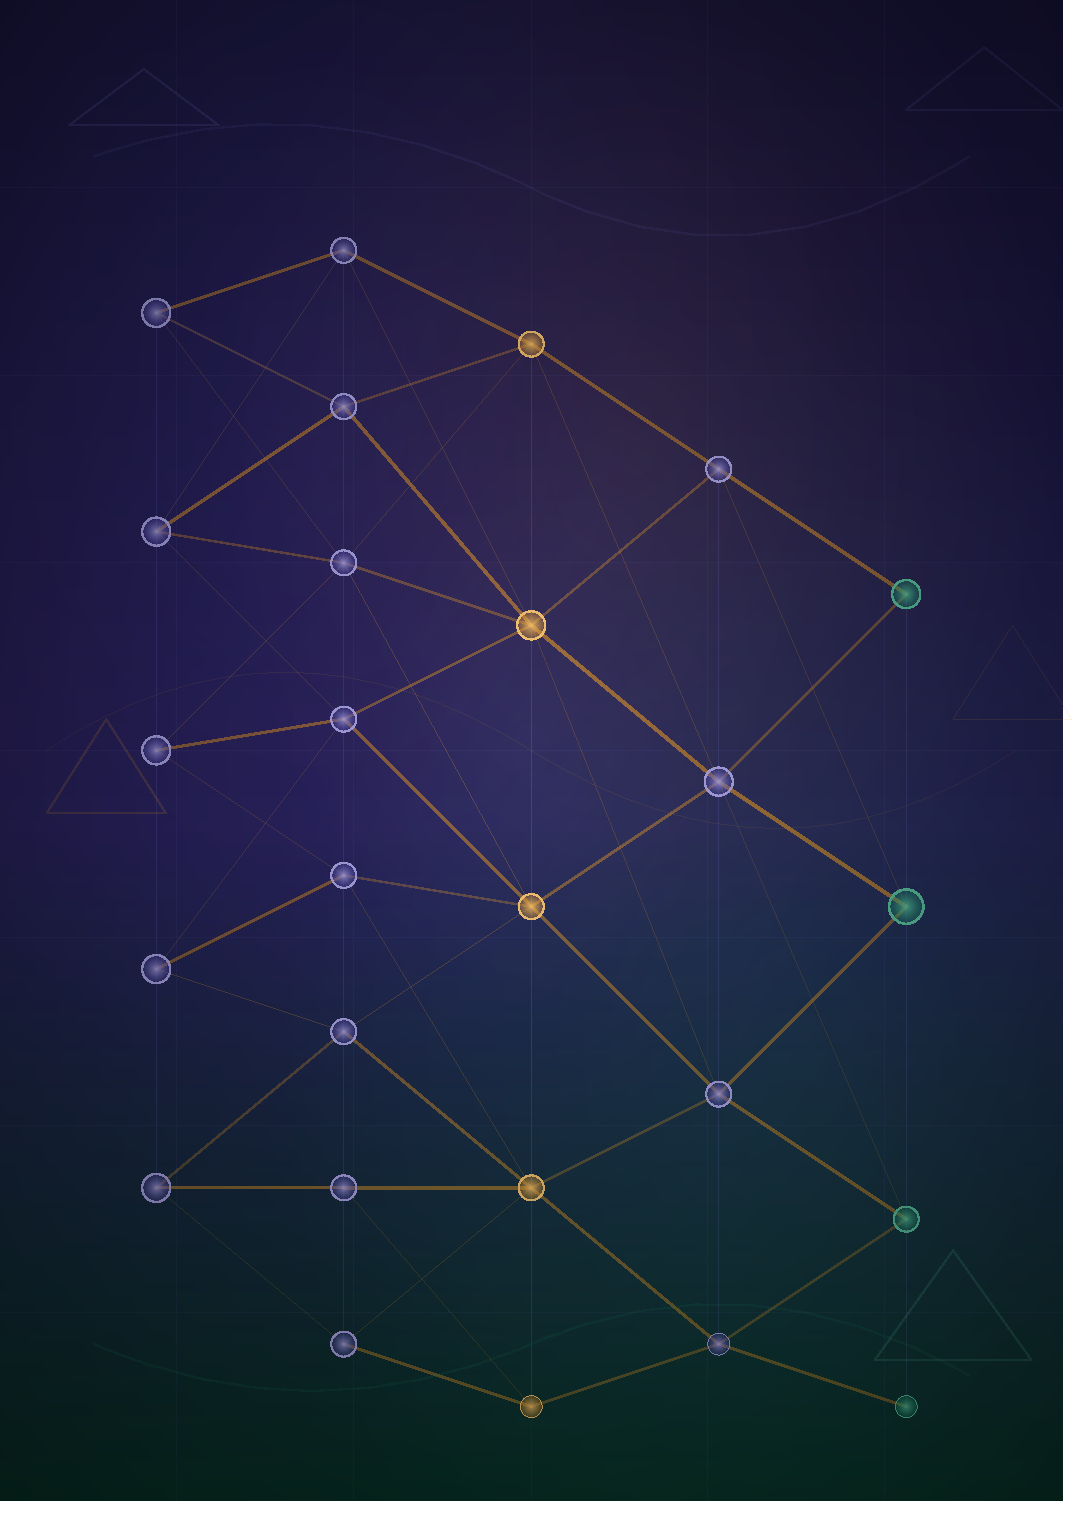
\includegraphics[scale=2]{phd_cover_background.pdf}%
    }
\begin{center}

\vspace*{.06\textheight}
{\scshape\LARGE \univname\par}\vspace{1.5cm} % University name
\textsc{\Large Doctoral Thesis}\\[0.5cm] % Thesis type

\HRule \\[0.4cm] % Horizontal line
{\huge \bfseries \ttitle\par}\vspace{0.4cm} % Thesis title
\HRule \\[1.5cm] % Horizontal line
 
% \begin{minipage}[t]{0.4\textwidth}
% \begin{flushleft} \large
% \emph{Author:}\\
% \href{http://www.johnsmith.com}{\authorname} % Author name - remove the \href bracket to remove the link
% \end{flushleft}
% \end{minipage}
% \begin{minipage}[t]{0.4\textwidth}
% \begin{flushright} \large
% \emph{Supervisor:} \\
% \href{http://www.jamessmith.com}{\supname} % Supervisor name - remove the \href bracket to remove the link  
% \end{flushright}
% \end{minipage}

\begin{minipage}[t]{0.45\textwidth}
\begin{flushleft} \large
\textbf{Author}\\
\authorname
\end{flushleft}
\end{minipage}
\begin{minipage}[t]{0.45\textwidth}
\begin{flushright} \large
\textbf{Supervisors}\\
\supname
\end{flushright}
\end{minipage}

\vspace{1.5cm}

\begin{center}
\large
\textbf{Reviewers}\\
Prof.\ Frank Kargl\\
Prof.\ Konrad Rieck
\end{center}

 
\vfill

\large \textit{A thesis submitted in fulfillment of the requirements\\ for the degree of \degreename}\\[0.3cm] % University requirement text
\textit{in the}\\[0.4cm]
\groupname\\\deptname\\[2cm] % Research group name and department name
 
\vfill

{\large \today}\\[4cm] % Date
%\includegraphics{Logo} % University/department logo - uncomment to place it
 
\vfill
\end{center}
\end{titlepage}

%----------------------------------------------------------------------------------------
%	DECLARATION PAGE
%----------------------------------------------------------------------------------------

% \begin{declaration}
% \addchaptertocentry{\authorshipname} % Add the declaration to the table of contents
% \noindent I, \authorname, declare that this thesis titled, \enquote{\ttitle} and the work presented in it are my own. I confirm that:

% \begin{itemize} 
% \item This work was done wholly or mainly while in candidature for a research degree at this University.
% \item Where any part of this thesis has previously been submitted for a degree or any other qualification at this University or any other institution, this has been clearly stated.
% \item Where I have consulted the published work of others, this is always clearly attributed.
% \item Where I have quoted from the work of others, the source is always given. With the exception of such quotations, this thesis is entirely my own work.
% \item I have acknowledged all main sources of help.
% \item Where the thesis is based on work done by myself jointly with others, I have made clear exactly what was done by others and what I have contributed myself.\\
% \end{itemize}
 
% \noindent Signed:\\
% \rule[0.5em]{25em}{0.5pt} % This prints a line for the signature
 
% \noindent Date:\\
% \rule[0.5em]{25em}{0.5pt} % This prints a line to write the date
% \end{declaration}

\begin{declaration}
\noindent I, \authorname, declare that this thesis titled:

\begin{center}
    {\bfseries \ttitle}
\end{center}

\noindent is the product of my own independent work and that I have used no sources 
or materials other than those specified. The passages taken from other works, 
either verbatim or paraphrased in the spirit of the original quote, are identified 
in each individual case by indicating the source.

\noindent I further declare that all my academic work was written in line with the principles 
of proper academic research according to the official ``Satzung der Universität 
Ulm zur Sicherung guter wissenschaftlicher Praxis'' (University Statute for the 
Safeguarding of Proper Academic Practice).

\vspace{3cm}

Munich, \hfill \rule{5cm}{0.4pt}

\hfill {\small \authorname, student number}

\end{declaration}


%	ACKNOWLEDGEMENTS
%----------------------------------------------------------------------------------------

\begin{acknowledgements}
\addchaptertocentry{\acknowledgementname} % Add the acknowledgements to the table of contents
This dissertation would not have been possible without the support of many people to whom I owe a great deal of gratitude.

First of all, I would like to thank my family. My father and mother have supported me since the very first days of my life, long before this PhD was even a distant thought, and their unwavering belief in me has been a quiet but constant source of strength throughout this journey. I also would like to express my deepest gratitude to my wife, Flan Ermine, whose patience, encouragement, and love have meant more than words can express. Having her by my side during the most demanding moments of this work made all the difference.

I am deeply grateful to my supervisors, Frank Kargl, Theo Dimitrakos, and Houda Labiod, for their guidance, availability, and trust throughout this research. Each of them brought a distinct and complementary perspective that shaped the direction and depth of this work in meaningful ways. I would also like to extend special thanks to Yannis, who, though not formally listed as a supervisor, was fully present in that role. His advice, feedback, and engagement were invaluable, and this dissertation is richer for his involvement. Beyond the scope of this PhD, Yannis also took the time to share life advice that helped me grow as a person, and for that I am especially grateful.

Among my colleagues, I owe particular thanks to Hussein Joumaa, the best friend I had at the office. Our conversations about everything and nothing were a constant source of relaxation and perspective. I am also grateful to Ana Petrovska, who helped me improve my writing and collaborated with me on several internal projects and publications, and to Gabriele, for the many insightful technical discussions on Subjective Logic and neural networks.

I also acknowledge the collaborators from outside Huawei, particularly from the University of Luxembourg: Gabriele Lenzini and Hüseyin Demirci, whose contributions enriched this work.

Finally, I am grateful to the friends who supported me both technically and morally throughout this PhD. Hugues Kouakou, Dro Sigui, and Adou Seka were fellow PhD students with whom it was invaluable to share the experience and realize we were all facing the same challenges. Alex N'guettia was always available and helped me with many tasks both personal and academic. Camara Yoane also helped with many personal matters and gave me the space to focus on this work. David and Cheick supported me since the very beginning of this journey.


\begin{comment}
    \begin{itemize}
    \item Family: Dad, Mom, who supported since my first days at school. at the really begining of my life/ and my Wife Flan Ermine now
    \item Supervisors: Frank Kargl, Theo Dimitrakos, Houda Labiod
    \item Yannis who was also a supervisor even unformally
    \item Colleague: Hussein Joumaa (The best friend I had at the office, talking about everything and any thing, help to relax and change my mind), Ana Petrovska  (helped me to improve my writings and collaborated with me on several works internally and papers) , Gabriele (very insighfull technical discussion on subjective logic and neural networks)
    \item Collaborators from outside huawei especially the university of luxembourg: Gabriele Lenzini, Hüseyin Demirci
    \item Friends who supported me, both technically and morally: Hugues Kouakou, Dro Sigui and Adou Seka another phd students with whom it was really useful to discuss and see that we are facing the same problem as phd student, Alex N'guettia gave me useful and helped me for many personal tasks and was always available to help, Camara Yoane helped me for many personal tasks. 
    \item All the other friends namely david, Cheick .. who also supported me since the begining of my Phd. 
\end{itemize}

\end{comment}

\end{acknowledgements}


%----------------------------------------------------------------------------------------
%	ABSTRACT PAGE
%----------------------------------------------------------------------------------------

\begin{abstract}
\noindent\enquote{\itshape There are no facts, only interpretations.}\bigbreak
\addchaptertocentry{\abstractname} % Add the abstract to the table of contents
\hfill Friedrich Nietzsche
\\
\\
Neural networks are increasingly deployed in high-stakes domains where the reliability of predictions has direct consequences. However most evaluation practices focus on aggregate performance metrics, which neither distinguish sources of uncertainty nor capture how trustworthiness propagates across the stages of a learning pipeline. This thesis addresses this gap by developing a formal, interpretable, and operational methodology for trust assessment in classifier neural network pipelines, grounded in Subjective Logic (SL). The framework comprises four contributions. First, a General Trust Assessment Methodology formalizes trust evaluation as a three-phase process (expression generation, atomic-opinion quantification, and expression evaluation), and an optimized Trust Network Analysis algorithm ensures computational efficiency and consistency of SL inference over complex graph structures. Second, the Parallel Trust Assessment System (PaTAS) operationalizes trust assessment across the full machine learning pipeline: a dataset trustworthiness module quantifies evidence quality at the training stage, and a trust propagation module mirrors neural network computations to carry trust from inputs through parameters to predictions, without modifying the underlying model. Third, a calibration-based trust formulation enables trust assessment in black-box settings using only observable model inputs and outputs. Fourth, an end-to-end evaluation on a 5G network energy classification task demonstrates that PaTAS trust opinions consistently discriminate between correct and incorrect predictions under controlled data quality variation, and produce signals coherent with the complementary calibration-trust view. Together, these contributions establish trust as a first-class, auditable object in neural network systems, and provide both the theoretical foundations and practical tools for its representation, quantification, and propagation.
\end{abstract}

%----------------------------------------------------------------------------------------

%----------------------------------------------------------------------------------------
%	LIST OF CONTENTS/FIGURES/TABLES PAGES
%----------------------------------------------------------------------------------------

\setcounter{tocdepth}{1}
% \setcounter{tocdepth}{1}
\tableofcontents % Prints the main table of contents

%----------------------------------------------------------------------------------------
%	ABBREVIATIONS
%----------------------------------------------------------------------------------------

\chapter*{List of Acronyms}
\addcontentsline{toc}{chapter}{List of Acronyms}


\begin{acronym}[HTTP]
  \acro{AI}{Artificial Intelligence}
  \acro{ML}{Machine Learning}
  \acro{RQ}{Research Question}
  \acro{NN}{Neural Network}
  \acro{SL}{Subjective Logic}
  \acro{DST}{Dempster-Shafer Theory}
  \acro{DSPG}{Directed Series-Parallel Graph}
  \acro{STN}{Subjective Trust Network}
  \acro{V2V}{vehicle-to-vehicle}
  \acro{C-ITS}{Cooperative Intelligent Transportation Systems}
  \acro{TNA-SL}{Trust Network Analysis with Subjective Logic}
  \acro{UQ}{Uncertainty Quantification}
  \acro{BBA}{Basic Belief Assignment}
  \acro{PDF}{Probability Density Function}
  \acro{IMA}{Intersection Movement Assistance}
  \acro{PPS}{Parallel Path Subnetwork}
  \acro{NL}{Nesting Level}
  \acro{FNN}{Feedforward Neural Network}
  \acro{NNL}{Node Nesting Level}
  \acro{BNN}{Bayesian Neural Network}
  \acro{EDL}{Evidential Deep Learning}
  \acro{SLE}{Subjective Logic Encodings}
  \acro{SBA}{Sampling-Based Approach}
  \acro{SP-graph}{Series--Parallel Graph}
  \acro{OOD}{Out of Distribution}
\end{acronym}

%----------------------------------------------------------------------------------------
%	PHYSICAL CONSTANTS/OTHER DEFINITIONS
%----------------------------------------------------------------------------------------

% \begin{constants}{lr@{${}={}$}l} % The list of physical constants is a three column table

% % The \SI{}{} command is provided by the siunitx package, see its documentation for instructions on how to use it

% Speed of Light & $c_{0}$ & \SI{2.99792458e8}{\meter\per\second} (exact)\\
% %Constant Name & $Symbol$ & $Constant Value$ with units\\

% \end{constants}

%----------------------------------------------------------------------------------------
%	SYMBOLS
%----------------------------------------------------------------------------------------
\chapter*{List of Symbols and Notation}
\addcontentsline{toc}{chapter}{List of Acronyms}


\begin{symbols}{lll} % Include a list of Symbols (a three column table)

$a$ & distance & \si{\meter} \\
$P$ & power & \si{\watt} (\si{\joule\per\second}) \\
%Symbol & Name & Unit \\

\addlinespace % Gap to separate the Roman symbols from the Greek

$\omega$ & angular frequency & \si{\radian} \\

$e$ & edge\\

$P$ & PNPS \\

$v$ & Node \\

$\Omega$ & Univers \\
$\Theta$ & Neural Networks Model \\

$\mathbb{X}$ & Opinion State space \\
 $\odot$, is defined as &
\[
\omega_X^{A\&B} = \omega_X^A \odot \omega_X^B.
\] & constraint fusion \\
\end{symbols}

% \chapter*{List of Definition}
% \listoftheorems[ignoreall,show={definition}]
%----------------------------------------------------------------------------------------
%	DEDICATION
%----------------------------------------------------------------------------------------

% \dedicatory{For/Dedicated to/To my\ldots} 

%----------------------------------------------------------------------------------------
%	THESIS CONTENT - CHAPTERS
%----------------------------------------------------------------------------------------

\mainmatter % Begin numeric (1,2,3...) page numbering

\pagestyle{thesis} % Return the page headers back to the "thesis" style

% Include the chapters of the thesis as separate files from the Chapters folder
% Uncomment the lines as you write the chapters


% \part{Introduction and Background}
% \label{part:intro}
\chapter{Introduction}
\section{Research Context and Motivation}
\subsection{Why Trust in Neural Networks Matters?}
\label{sec:motivation}
% \sidenote{}
\marginpar{AI and NN importance.}
\ac{AI} has evolved into a general-purpose technology that serves 
as the foundation for a growing number of computational systems used to support or automate decision-making across diverse domains. Advances in data availability, computing power, and learning algorithms have enabled \ac{AI} systems to perform tasks that were traditionally considered to require human intelligence, including perception, pattern recognition, prediction, and planning. As a result, \ac{AI}-based systems are increasingly embedded in real-world processes that operate at scale and interact directly with individuals, organizations, and societies.

Within this broad landscape, \ac{ML}  has emerged as a dominant approach for building adaptive and data-driven \ac{AI} systems. Rather than relying on explicitly programmed rules, \ac{ML}  systems infer patterns and decision functions from data, allowing them to generalize to previously unseen inputs. This shift from rule-based systems to learned models has substantially expanded the scope and performance of \ac{AI} applications, while also reducing direct human control over internal decision logic.

\acfp{NN}, and in particular deep \acp{NN}, form the backbone of many state-of-the-art \ac{ML}  systems. Their expressive power and scalability have led to widespread adoption in applications where complex, high-dimensional data must be processed, such as computer vision, natural language processing, and sequential decision-making~\cite{Goodfellow-et-al-2016}. \acp{NN} are increasingly deployed in domains where their outputs influence decisions with significant consequences, including healthcare diagnostics~\cite{Shahid2019-eq}, financial prediction~\cite{NBERw31502}, and autonomous driving~\cite{10604830}. In such settings, incorrect or overconfident predictions may lead not only to technical failure but also to physical harm, economic loss, or violations of fundamental rights. As a result, the question of whether a \ac{NN} can be trusted has become as important as how accurately it performs.

\marginpar{Trust in \ac{AI}} 
Recent policy and regulatory efforts recognize trustworthiness as a foundational requirement for \ac{AI} systems. The Ethics Guidelines for Trustworthy \ac{AI} issued by the European Commission’s High-Level Expert Group define trustworthiness through three complementary components: lawful \ac{AI}, ethical \ac{AI}, and robust \ac{AI}~\cite{ec2019ethics}. 

Ethical \ac{AI} is grounded in four principles (see \cref{fig:tai}), namely respect for human autonomy, prevention of harm, fairness, and explicability, while robust \ac{AI} emphasizes technical reliability, safety, and resilience to uncertainty. These principles are further operationalized through concrete requirements such as transparency, accountability, and human oversight. Together, this framework establishes trustworthiness as a necessary condition for the deployment of \ac{AI} systems, rather than a desirable property.

\begin{figure}
    \centering
    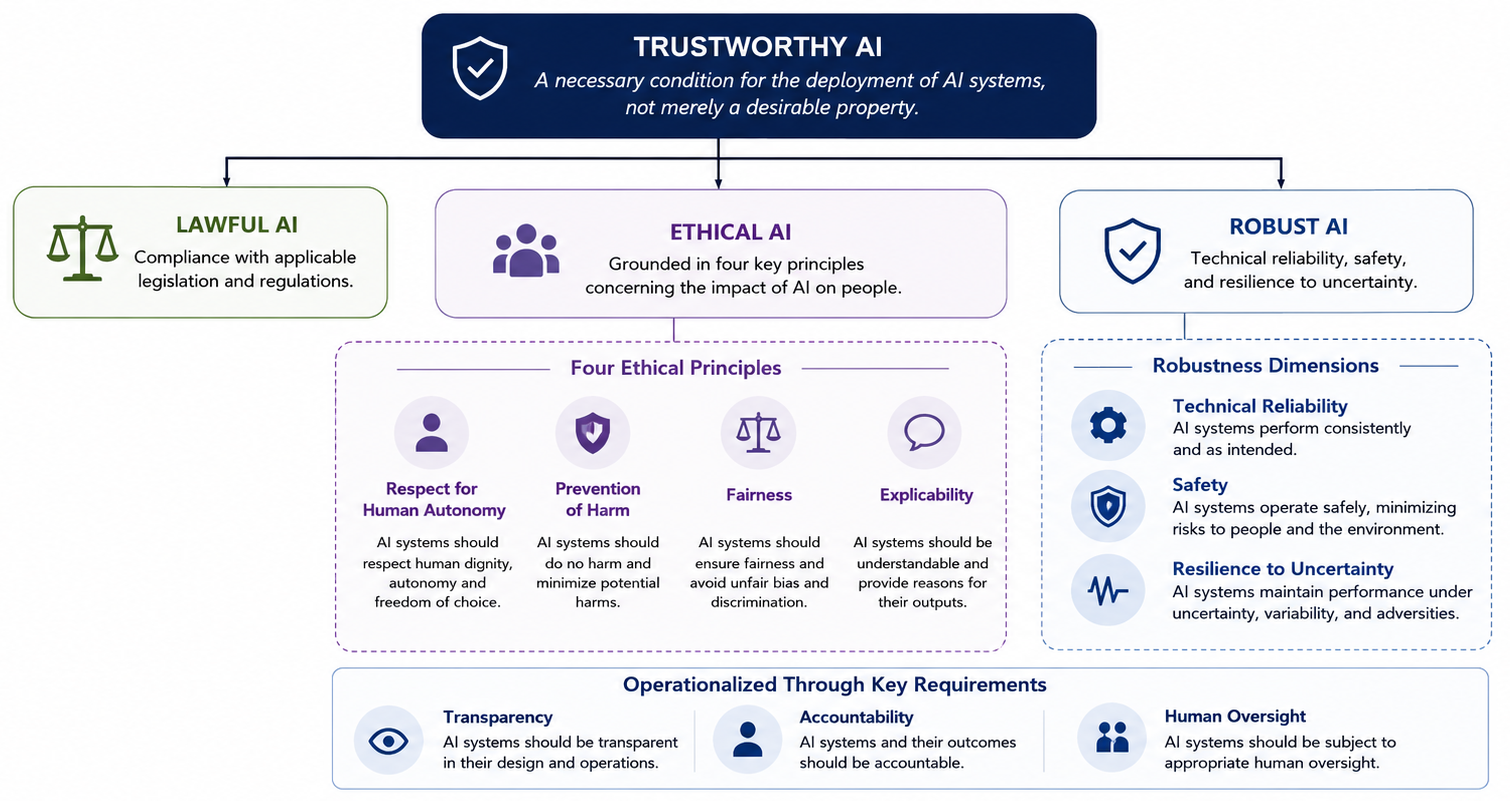
\includegraphics[width=0.8\linewidth]{Figures/TAI.png}
    \caption{Trustworthy AI framework~\cite{10.1145/3491209}}
    \label{fig:tai}
\end{figure}
%%%%%%%%%%%NEW DEB
\marginpar{Foundations of Trust}
From a conceptual perspective, trust is inherently linked to risk and vulnerability. In the organizational and behavioral sciences, trust is commonly defined as the willingness of a party to accept vulnerability to the actions of another under conditions of uncertainty and risk. In their seminal work, Mayer, Davis, and Schoorman formalize trust as the willingness of a trustor to be vulnerable to a trustee based on expectations regarding the trustee’s ability, benevolence, and integrity~\cite{55a601e8-f397-31d9-a222-5b5dd8d0bb15}. This definition emphasizes that trust is not merely a belief about expected outcomes, but a deliberate acceptance of potential negative consequences. It further distinguishes trust from related notions such as predictability or cooperation, which may exist without exposure to risk.

Beyond social and organizational contexts, the notion of trust has also been formalized in the domain of \ac{ICT} systems. In this setting, trust is not an abstract interpersonal concept but is defined as a relation between an agent and specific properties of a system, reflecting the agent’s belief that these properties hold within its perceived model of the system~\cite{10.1007/978-3-642-13446-3_14}. This perspective highlights two important aspects: first, trust is inherently subjective and depends on the agent’s knowledge and assumptions; second, trust is always tied to well-defined system properties, such as security guarantees or behavioral correctness.

\marginpar{Trust in Neural Networks}
These complementary perspectives provide a unified view of trust as both a risk-aware decision and an evidence-dependent relation to system properties. This conceptualization naturally extends to \ac{AI} systems. When a human user relies on the output of a \ac{NN}, for instance in medical diagnosis or automated decision-support, the user becomes vulnerable to errors, biases, and miscalibrated confidence estimates. At the same time, the user’s trust is implicitly grounded in assumptions about specific properties of the system, such as predictive reliability, robustness, and alignment with intended objectives. However, these properties are typically neither directly observable nor formally verifiable by the user.

Moreover, the internal decision-making processes of \acp{NN} are often opaque, limiting the user’s ability to monitor and validate individual predictions. As a result, reliance on such systems closely mirrors the trust relationships described in both organizational and formal \ac{ICT} settings: it involves accepting risk based on expectations about the system’s competence, reliability, and underlying assumptions. This dual nature of trust, as both vulnerability acceptance and property-based belief, highlights the need for formal, interpretable, and evidence-based approaches to trust assessment in \ac{NN} systems.

\marginpar{Limits of Current Metrics}
Despite this conceptual alignment, most existing approaches for evaluating \acp{NN} focus primarily on predictive performance metrics such as accuracy, precision, or recall. While these metrics are essential, they fail to capture whether a model is trustworthy in the sense required for high-stakes decision-making. A highly accurate model may still be unsafe if it is poorly calibrated, biased, or trained on unreliable data. Conversely, a model with lower predictive accuracy may be more trustworthy if it appropriately represents uncertainty and avoids overconfident predictions in unfamiliar or out-of-distribution scenarios.

Furthermore, trust in \acp{NN} is not solely a property of the model architecture or its learned parameters. It is inherently multi-layered and depends on the quality of the training data, the reliability of annotations, the behavior of the learning process, and the way uncertainty propagates from inputs to outputs. Dataset biases, labeling inconsistencies, and hidden correlations can undermine trust long before inference is performed. Without explicit mechanisms to assess and propagate trust across these components, users are left with opaque confidence scores that provide limited support for risk-aware decision-making.

These limitations motivate the need for a formal and interpretable framework for trust in \acp{NN}. Such a framework should explicitly represent uncertainty and support principled reasoning about how trust evolves as new information becomes available. It should also align with established theories of trust and risk, while remaining operational within modern \ac{ML} pipelines. This thesis addresses these requirements by grounding trust assessment in \acf{SL} and by developing mechanisms to quantify, propagate, and aggregate trust across datasets, network structures, and model outputs.


\subsection{Challenges in Quantifying Trust and Uncertainty in Neural Networks}
\label{sec:quantification_challenges}
Although the need for trust in \ac{NN} based systems is increasingly acknowledged, the quantification of trust and uncertainty remains an open and challenging problem. Unlike classical performance metrics, trust is not directly observable and cannot be measured through a single empirical quantity. Instead, it emerges from a combination of evidence, uncertainty, and risk, all of which must be represented in an interpretable manner.

A first challenge concerns the absence of a clear and unified definition of trust in the context of \acp{NN}. In practice, trust is often implicitly equated with predictive accuracy, confidence scores, or reliability estimates. However, these quantities capture only limited aspects of trust and do not account for the conditions under which a system may fail or behave unpredictably. Without a formal definition that distinguishes trust from related concepts, quantitative assessments remain inconsistent and difficult to assess across models and application domains.

A second challenge relates to the representation of uncertainty. Most \acp{NN} produce probabilistic outputs that are commonly interpreted as measures of confidence. However, such probabilities do not distinguish between uncertainty arising from insufficient evidence and uncertainty caused by conflicting evidence. For example, a prediction based on few training examples and a prediction derived from strongly disagreeing labels may both result in similar probability values, despite reflecting fundamentally different situations. This limitation complicates the interpretation of model outputs and limits their usefulness for risk-aware decision-making.

A third challenge lies in the quantification of trust at different levels of abstraction. Trust may be defined at the level of individual predictions, model components, datasets, or entire learning pipelines. Existing evaluation practices predominantly assess models at an aggregate level, relying on global performance metrics that obscure variation in trust and uncertainty across individual outputs. Consequently, predictions that are ambiguous or weakly supported by data are often treated equivalently to those that are well-supported. Addressing this limitation requires methods that can represent and evaluate trust at a finer granularity.

Another challenge concerns the integration of data quality into trust assessments. \acp{NN} are highly sensitive to the quality of training data, yet data-related issues such as labeling noise, annotator disagreement, and sampling bias are rarely incorporated into quantitative trust measures. In many cases, uncertainty introduced during data collection is not modeled and remains invisible at inference time. While these factors implicitly influence model behavior through training, their lack of explicit representation creates a disconnect that makes it difficult to reason about how much confidence should be placed in predictions derived from unreliable or contentious data.

Finally, there is a challenge associated with the propagation and aggregation of trust. In complex \ac{NN} architectures, trust assessments derived from different sources, such as data quality or component reliability, must be combined to form an overall judgment. Standard probabilistic frameworks offer limited support for such aggregation, particularly when sources of evidence are heterogeneous or partially dependent. Without principled operators for combining and propagating trust, quantitative assessments risk being inconsistent or misleading.

These challenges illustrate that quantifying trust and uncertainty in \acp{NN} requires more than probabilistic prediction and performance evaluation. It calls for representations that explicitly encode evidence, disagreement, and ignorance, and for reasoning mechanisms that support consistent propagation and aggregation of trust across system components. Addressing these challenges is the central objective of this thesis.

\section{Problem Statement and Research Questions}

This thesis aims to develop a formal, interpretable, and operational framework for assessing trust in \ac{NN} pipelines, both during training and inference. In particular, such framework should model how trust propagates from the training data to the learned model parameters, and from input observations to output predictions through the model. While traditional evaluation approaches primarily rely on predictive performance, they fail to capture essential aspects of trust such as uncertainty, incomplete knowledge, and the reliability of information sources. As \ac{NN} systems become increasingly complex and are deployed in safety-critical and open environments, these limitations become more pronounced.

To address this gap, this work investigates how trust can be modeled as an evidence-based quantity and systematically integrated across the different stages of the \ac{ML} system pipeline. In particular, the thesis explores how \ac{SL} can be adapted and used to represent, quantify, and combine trust in \ac{NN} systems. This includes assessing the trustworthiness of training datasets, modeling the propagation of trust through structured dependencies, and evaluating black-box models through observable signals such as calibration behavior.

The objective is therefore to provide a unified methodology that enables practical computation, interpretation, and use in real-world \ac{ML} systems. Based on these objectives and the challenges identified earlier, we formulate the following research questions.

\subsection{Part I: Efficient and Consistent Trust Inference with \aclu{SL}}
While \ac{SL} provides a formal and well-established framework for representing and combining uncertain information, its direct application to complex systems raises important challenges. In particular, performing trust inference over large and complex graphs can lead to significant computational overhead, as the number of operations required to propagate and aggregate opinions grows rapidly with the size and architecture of the system. This limits the scalability of existing approaches in realistic settings.

In addition to these computational challenges, existing \ac{SL} frameworks may lead to a loss of information during trust inference. In particular, successive transformations and unnecessary reduction operations can degrade the quality of the inferred trust values, resulting in less robust and less reliable trust quantification.

Finally, the process of propagating subjective opinions across such graphs may lead to inconsistencies, where the resulting trust assessments depend on the structure of the graph or the order in which operations are applied. This lack of stability undermines the reliability and interpretability of the inferred trust values.




These limitations restrict the applicability of \ac{SL} in complex systems where trust must be evaluated over interconnected components. Therefore, there is a need to define methods that reduce computational overhead, improve the robustness of trust quantification, and ensure the consistency of trust inference when applied to such settings.

This leads to the first research question:
\begin{rqbox}{Efficient and Consistent Trust Inference}
\label{rq:1}
    How can computational efficiency and consistency be ensured when performing trust inference with \ac{SL} over complex graphs?
\end{rqbox}


\subsection{PART II: Trustworthiness of Training Datasets}
Beyond the design of a formal framework for trust representation and propagation, trust in \ac{ML} systems is fundamentally influenced by the quality and reliability of the data used during training. In particular, training datasets serve as the primary source of evidence from which models learn, making their trustworthiness a critical factor in the overall behavior of the system.

However, existing approaches for dataset evaluation are often limited to statistical quality measures, bias detection metrics, or performance-based validation. While these methods provide useful insights, they do not offer a unified and interpretable way to quantify trust in datasets as an explicit function of evidence, uncertainty, and data reliability. Moreover, they typically fail to capture the impact of incomplete, noisy, or conflicting information, which is inherent in real-world data.

This creates a fundamental gap: although data is the foundation of learning, there is no framework to represent and quantify its trustworthiness in a way that is consistent with subsequent stages of trust assessment in the learning and inference processes. In particular, datasets are rarely modeled as structured sources of evidence that can be integrated into a broader trust reasoning framework.

Therefore, it is necessary to develop a method for assessing dataset trustworthiness that is both formally grounded and compatible with evidence-based trust modeling.

This leads to the second research question:
\begin{rqbox}{Trustworthiness of Training Datasets}
    How can the trustworthiness of training datasets be formally represented and quantified within an evidence-based framework?
\end{rqbox}

\subsection{PART III: Trust Propagation in \aclu{NN}s from Training Dataset to Inference}
Building upon the representation of trust and the quantification of dataset trustworthiness, a central challenge lies in understanding how trust propagates throughout the learning and inference processes. In \ac{ML} systems, trust is not confined to isolated components, but instead evolves across multiple stages, from the training data to the learned model parameters, and from input observations to output predictions.

During training, model parameters are inferred from data, implicitly inheriting the uncertainty, noise, and potential biases present in the dataset. Similarly, during inference, predictions are generated through complex transformations of the input, where uncertainty is accumulated and propagated throughout the model. Despite this, existing approaches typically assess trust at a single stage, either at the level of data, model performance, or output confidence, without providing a unified view of how trust flows across the entire pipeline.

This lack of continuity prevents a consistent interpretation of trust, as it remains unclear how uncertainties originating from the data influence the learned model, and how they subsequently affect predictions. Therefore, a key challenge is to establish a mechanism for modeling and quantifying the propagation of trust across both the learning and inference processes.

This leads to the third research question:
\begin{rqbox}{Trust Propagation from Training Dataset to Inference}
    How can trust be consistently propagated from training data to learned model parameters, and from inputs to outputs during inference, within an evidence-based framework?
\end{rqbox}
In practice, however, this assumption of full model transparency does not always hold, as many modern \ac{ML} models operate as black-box systems where internal parameters and intermediate computations are not accessible. While the propagation-based framework remains essential for understanding trust at a system level, this limitation motivates the need for complementary approaches that rely only on observable signals. This raises an important extension of the research question:
\begin{rqbox}{Trust Assessment under Limited Observability}
    how can trust be assessed when only observable data, such as model outputs are available?
\end{rqbox}



\section{Contributions of the Thesis}

This thesis introduces a unified and operational framework for trust assessment in \ac{ML} systems, with a particular focus on neural network pipelines. Building upon the research questions formulated in the previous section, the contributions of this work span the representation, quantification, and propagation of trust, as well as its practical evaluation in realistic settings. The main contributions are summarized as follows:

\begin{enumerate}
    \renewcommand{\labelenumi}{C\arabic{enumi}}
    \item \label{c:1}\textbf{A general methodology for trust assessment~\cite{5gaa_trust4cav_2025,connect_d31_taf}.}  
    This thesis proposes a \emph{General Trust Assessment Methodology} that formalizes trust as an evidence-based reasoning process. The methodology provides a structured framework for defining trust expressions, collecting and modeling evidence, and evaluating trust in a consistent and interpretable manner. It serves as a unifying backbone that can be instantiated across different components of a \ac{ML} pipeline.

    \item \label{c:2}\textbf{A scalable, consistent, and more robust framework for trust inference using Subjective Logic~\cite{10.1007/978-3-032-08887-1_4,10706345}.}  
    To address the limitations of applying \ac{SL} to complex systems, this work introduces methods that ensure computational efficiency, more robust trust quantification, and consistency of inference over large and complex graphs. In particular, it proposes an optimized graph analysis framework that enables stable, information-preserving, and scalable propagation of subjective opinions.

    \item \label{c:3}\textbf{A formal approach for assessing the trustworthiness of training datasets~\cite{ecmldatatrust,trust-aidatatrust}.}  
    This thesis develops a method to model training datasets as sources of evidence and to quantify their trustworthiness within an evidence-based framework. The approach captures uncertainty, noise, and potential biases in the data, allowing dataset quality to be explicitly integrated into the overall trust assessment process.

    \item \label{c:4}\textbf{A unified framework for trust propagation across learning and inference processes~\cite{patas}.}  
    A key contribution of this work is the formalization of trust propagation throughout the \ac{ML} pipeline. The proposed approach models how trust evolves from training data to learned model parameters, and from inputs to outputs during inference, providing a consistent and end-to-end view of trust in the system.

    \item \label{c:5}\textbf{A method for trust assessment in black-box models based on output data~\cite{11124121}.}  
    Recognizing that modern \ac{ML} systems often operate as black boxes, this thesis proposes an extension of the trust assessment framework that relies on observable quantities, such as calibration behavior. This enables the quantification of trust even when internal model information is not accessible, bridging the gap between theoretical modeling and certain practical deployment.
    
    \item \label{c:6}\textbf{An end-to-end evaluation on a real-world use case.}  
    The proposed framework is evaluated on a practical use case involving device energy consumption estimation. This evaluation demonstrates the applicability of the methodology in a realistic setting and highlights its ability to provide meaningful and interpretable trust assessments across the full pipeline.
\end{enumerate}
\begin{figure}
    \centering
    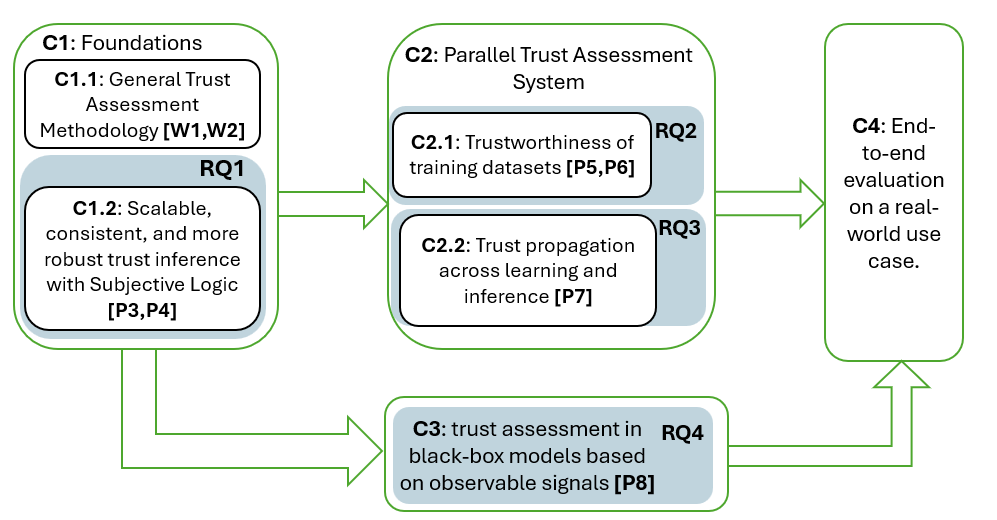
\includegraphics[width=0.9\linewidth]{Figures/contribution.png}
    \caption{overview of the main contributions of this thesis}
    \label{fig:contributions}
\end{figure}

\cref{fig:contributions} provides an overview of the main contributions of this thesis and their relationships. The contributions are organized into three conceptual layers, namely the foundations layer, the data and propagation layer, and the deployment layer. The figure highlights that the proposed General Trust Assessment Methodology (C\ref{c:1}) and the scalable trust inference framework (C\ref{c:2}) form the basis for subsequent developments, with (C\ref{c:2}) constituting a component of (C\ref{c:1}). It further illustrates that dataset trustworthiness (C\ref{c:3}) and trust propagation (C\ref{c:4}) are integrated within a unified pipeline, and that the general methodology extends to practical settings through black-box trust assessment (C\ref{c:5}) and the dataset trustworthiness assessment(C\ref{c:3}). Finally, it shows that both (C\ref{c:4}) and (C\ref{c:5}) extend to an end-to-end evaluation (C\ref{c:6}). The mapping to the research questions is also indicated, emphasizing the coherence between the problem formulation and the proposed contributions.



\section{Contributions of the Thesis}

This thesis proposes a unified and operational framework for trust assessment in \ac{ML} systems, with a particular focus on neural network pipelines. 
The contributions are structured into four main components, corresponding to the research questions and the different layers illustrated in \cref{fig:contributions}.

\subsection{Foundations: Trust Representation and Inference (C1)}

The first contribution establishes the theoretical and methodological foundations required to represent and reason about trust in complex systems. It is structured into two complementary sub-contributions addressing trust inference.

\textbf{C1.1 -- General Trust Assessment Methodology (\cref{chap:Trust_method})\cite{connect_d31_taf,5gaa_trust4cav_2025}.}  
This work introduces a general methodology for trust assessment based on evidence and structured reasoning. It formalizes trust as an explicit and interpretable process composed of (i) trust expression generation, (ii) atomic trust opinion quantification, and (iii) expression evaluation using \aclu{SL} operators. 
This contribution provides a domain-agnostic framework that serves as the backbone of all subsequent developments and addresses the need for a formal definition of trust in AI systems.

\textbf{C1.2 -- Scalable and Consistent Trust Inference Framework (\cref{chap:tnasl})~\cite{10.1007/978-3-032-08887-1_4}.}  
To enable the practical application of the methodology to complex systems such as \aclu{NN}, this thesis proposes an optimized trust inference framework. In particular, it introduces improved algorithms for Trust Network Analysis that ensure computational efficiency, reduce information loss, and guarantee consistency of inference results. This contribution directly addresses \textbf{RQ1} by enabling scalable and stable trust reasoning over complex dependency structures.

\subsection{Parallel Trust Assessment System (C2)}

The second contribution introduces a system-level framework that operationalizes trust assessment across the full \ac{ML} pipeline.

\textbf{C2 -- Parallel Trust Assessment System Overview (\cref{chap:ovl}).}  
This thesis proposes the \acf{PaTAS}, a framework that operates alongside \ac{NN} to assess trust without modifying their internal computations. \ac{PaTAS} provides a unified architecture that connects dataset trustworthiness, parameter reliability, and inference-time trust into a single coherent pipeline. It is structured around two main components: (i) a \emph{trust quantification layer}, which models trust in data and labels, and (ii) a \emph{trust propagation layer}, which mirrors \ac{NN} computations to propagate trust from dataset to model parameters during training and from inputs to outputs during inference.

\textbf{C2.1 -- Trustworthiness of Training Datasets (\cref{chap:data})~\cite{ecmldatatrust,trust-aidatatrust}.}  
A formal approach is developed to model datasets as structured sources of evidence and to quantify their trustworthiness using Subjective Logic. 
This contribution enables the assessment of dataset-level properties such as bias and reliability under uncertainty, including cases with incomplete or conflicting evidence. It directly addresses \textbf{RQ2} by providing a principled and interpretable framework for dataset trust quantification.

\textbf{C2.2 -- Trust Propagation Across Learning and Inference (\cref{chap:patas})~\cite{patas}.}  
Building on dataset trust, this work introduces mechanisms to propagate trust throughout the neural network, from training data to model parameters and from inputs to outputs during inference. 
The proposed PaTAS framework defines trust nodes and trust functions that mirror neural computations and enable end-to-end trust propagation.  
This contribution addresses \textbf{RQ3} by providing a consistent and operational solution for trust propagation across the entire ML lifecycle.

\subsection{Trust Assessment in Black-Box Models (C3)}

\textbf{C3 -- Trust Assessment under Limited Observability (\cref{chap:bb})~\cite{11124121}.}  
Recognizing that many real-world systems operate as black boxes, this thesis proposes a method to assess trust based solely on observable signals, such as model outputs and calibration behavior. 
This approach enables trust evaluation without access to internal model parameters or architecture, thereby extending the applicability of the framework to practical deployment scenarios.  
This contribution addresses \textbf{RQ4} by enabling trust assessment under limited observability.

\subsection{End-to-End Evaluation (C4)}

\textbf{C4 -- Real-World End-to-End Evaluation (\cref{chap:usecase}).}  
Finally, the proposed framework is validated through an end-to-end use case involving a real-world application. 
This evaluation demonstrates how the different components of the framework interact in practice and shows that the proposed approach provides meaningful, interpretable, and actionable trust assessments across the full AI pipeline.

\begin{figure}
    \centering
    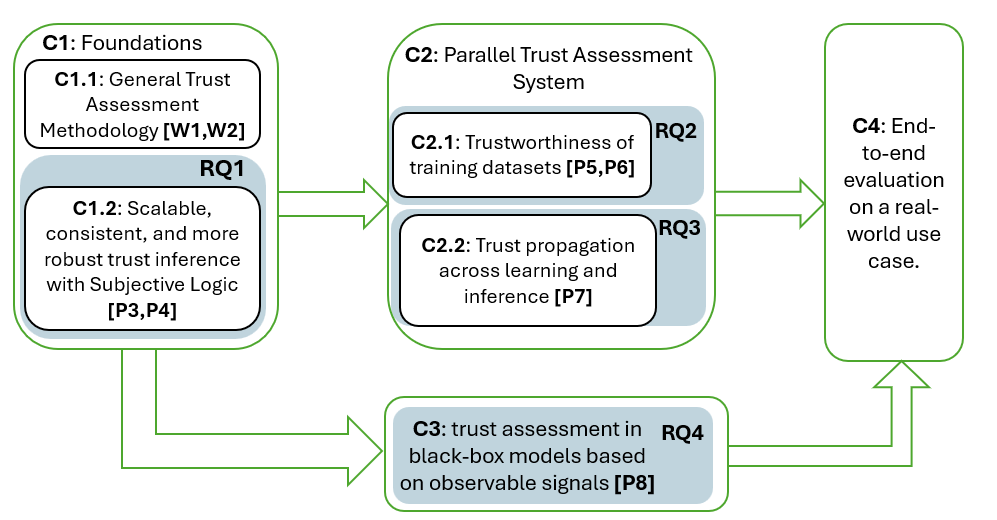
\includegraphics[width=0.9\linewidth]{Figures/contribution.png}
    \caption{overview of the main contributions of this thesis}
    \label{fig:contributions}
\end{figure}


Overall, these contributions form a coherent framework that enables the representation, quantification, propagation, and evaluation of trust in neural network systems. They collectively address the research questions defined in this thesis and provide both theoretical foundations and practical tools for trustworthy AI.

\cref{fig:contributions} presents an overview of the main contributions of this thesis and their relationships, structured according to the research questions. The contributions are organized into three conceptual layers: (i) the foundations layer (C1), (ii) the system and propagation layer (C2), and (iii) the deployment and evaluation layer (C3--C4).

At the foundation level, C1 establishes the theoretical and methodological basis for trust assessment. It combines a general trust assessment methodology (C1.1) with a scalable and consistent trust inference framework (C1.2), addressing \textbf{RQ1}. These components form the core building blocks upon which all subsequent contributions rely.

Building on these foundations, C2 introduces the Parallel Trust Assessment System, which operationalizes trust assessment across the machine learning pipeline. This component is decomposed into two complementary sub-contributions: dataset trustworthiness assessment (C2.1), addressing \textbf{RQ2}, and trust propagation across learning and inference (C2.2), addressing \textbf{RQ3}. Together, they form a unified pipeline that links data, model parameters, and predictions through consistent trust modeling and propagation.

In parallel, C3 extends the framework to settings where internal model information is not accessible. By relying solely on observable signals, it enables trust assessment in black-box models and addresses \textbf{RQ4}. This component complements the propagation-based approach by ensuring applicability of the methodology in black box deployment scenarios.

Finally, C4 integrates the different components into an end-to-end evaluation on a real-world use case. 
It demonstrates how trust can be assessed across the full pipeline, from data to inference, and validates the coherence and applicability of the proposed framework.



\section{Structure of the Thesis}

This dissertation is organized into several chapters that progressively develop a unified framework for trust assessment in \ac{NN} systems, spanning from theoretical foundations to practical instantiations across the \ac{NN} pipeline.

\cref{chap:rw} presents the theoretical foundations and related work. It reviews existing approaches for reasoning under uncertainty, including probabilistic methods, \aclu{DST}, and \ac{SL}. It also surveys prior work on trust and uncertainty in \acp{NN}, covering dataset quality and uncertainty quantification.The chapter concludes with a synthesis of the limitations of existing approaches, motivating the research questions addressed in this thesis.

\cref{chap:Trust_method} introduces the \emph{General Trust Assessment Methodology}, which forms the conceptual backbone of this dissertation. It formalizes trust as an evidence-based reasoning process structured around three main steps: (i) the generation of trust expressions through the decomposition of high-level trust propositions, (ii) the quantification of atomic trust opinions from available evidence, and (iii) the evaluation of these expressions using \ac{SL} operators. This methodology is designed to be domain-agnostic and serves as a unifying framework that forms the basis for all subsequent contributions.

\cref{chap:tnasl} focuses on the efficient and correct realization of the proposed methodology. It introduces an optimized \aclu{TNA-SL}, which enables the generation of trust expressions through structured graph-based representations. This chapter provides the theoretical and algorithmic foundation required to process complex graph in a consistent, robust and scalable manner.


\cref{chap:ovl} provides an overview of the \acf{PaTAS}, introducing a unified perspective on trust assessment across the different stages of the \ac{ML} pipeline. It presents the overall architecture of the proposed framework and outlines how trust can be analyzed from training data to model behavior during inference. In particular, this chapter identifies the key components involved in trust evaluation, including dataset-related factors, training processes, and inference mechanisms. It therefore serves as a system-level view that bridges the theoretical foundations and the subsequent detailed developments.



\cref{chap:data} instantiates the general methodology at the level of training data by addressing dataset trustworthiness. It focuses on the quantification of trust in datasets through properties such as labeling reliability and bias. Using \ac{SL}, the chapter treats datasets as structured sources of evidence and proposes methods to quantify their reliability, uncertainty, and potential biases
within an evidence-based framework. This chapter demonstrates how the proposed methodology can be applied to assess the reliability of data, which constitutes the foundation of any \ac{ML} system.

\cref{chap:patas} introduces the technical realization of the trust propagation layer within the \ac{PaTAS}. Building upon the dataset trustworthiness assessment, it integrates these inputs into the trust evaluation process and enables end-to-end computation of trust across the learning and inference stages. This chapter demonstrates how the different components of the framework interact in practice and how trust can be consistently propagated throughout the system.

\cref{chap:usecase} presents a use case illustrating the application of the proposed methodology in a real-world scenario. It demonstrates how trust can be assessed across different components of a system and highlights the practical relevance of the framework.

\cref{chap:bb} addresses the problem of trust assessment in black-box models. It proposes a calibration-based approach to quantify trust using observable signals, allowing trust evaluation when internal model information is not accessible. This chapter extends the work to support certain practical deployment settings.

Finally, \cref{chap:conclusion} summarizes the main contributions of the thesis and discusses limitations, perspectives, and directions for future work.


















\chapter{Background and Related Work [By End of March]}
% \todo[inline]{Estimated Nb Pages: 11 - 13}
\section{Reasoning under uncertainty}
% \todo[inline]{To be read again, and check the references}
\subsection{Probabilistic and Bayesian Theory}

When assuming an objective and fully observable setting, classical binary logic can be used to assert propositions about the state of a variable as either true or false~\cite{boole1847mathematical}. For example, let $X$ be a binary variable representing the operational status of a sensor, where $X = 1$ denotes ``functional'' and $X = 0$ denotes ``faulty''.  If the internal state of the sensor is fully observable and reliable diagnostic information is available, the proposition ``the sensor is functional'' can be asserted as either true or false with certainty. However, real-world systems are rarely fully observable or deterministic. In many practical situations, the truth value of a proposition cannot be determined with certainty due to inherent variability, incomplete information, or limited observations.

Probability logic~\cite{vonNeumann1956ProbabilisticLogics,Nilsson1986ProbabilisticLogic} extends binary logic by allowing propositions to take truth values in the continuous interval $[0,1]$, thereby modeling uncertainty. 
A probability value can be interpreted as the likelihood that a proposition holds, enabling partial truth assignments and quantitative reasoning under uncertainty. The probability theory has proven highly effective for modeling randomness and variability in complex systems. However, it implicitly assumes that probability values themselves are known or can be reliably estimated from sufficient evidence.

In practice, this assumption is often violated. Probabilities are typically inferred from finite data, subjective judgment, or imperfect measurements, which introduces an additional layer of uncertainty that standard probability theory does not explicitly represent. Moreover, probability assignments are usually observer-dependent: they reflect the belief of an individual or system given its available information, rather than an objective property of the world.

Bayesian theory~\cite{gelman2013bayesian,jaynes03,Bernardo:1319894} addresses some of these challenges by treating probabilities as degrees of belief (given the knowledge) and updating them through Bayes’ rule as new evidence becomes available. Bayesian inference provides a mechanism for incorporating prior knowledge and observational data, and it is widely used in statistics and machine learning~\cite{barberBRML2011}. Nonetheless, Bayesian probability remains a single-layer uncertainty framework: uncertainty is encoded solely in probability distributions over random variables.

This limitation becomes apparent when distinguishing between uncertainty due to inherent randomness of a variable (aleatoric uncertainty) and uncertainty due to lack of knowledge or insufficient evidence (epistemic uncertainty). Reconsider the binary sensor variable $X \in \{0,1\}$, where $X=1$ denotes that the sensor is functional and $X=0$ denotes that it is faulty. An observer who has access to zero information may assign $P(X=1) = P(X=0) =0.5$, reflecting uncertainty about the sensor’s state as he has none information. Another observer may possess detailed information: for example, evidence that the sensor hardware is new and properly calibrated (supporting $X=1$), combined with recent intermittent signal dropouts or abnormal readings (supporting $X=0$). When these pieces of evidence are considered together, this observer may also assign $P(X=1)=P(X=0)=0.5$, but for a fundamentally different reason namely, the presence of conflicting evidence rather than pure ignorance.

The probability value captures uncertainty about the sensor state itself, but it does not encode uncertainty about the reliability of the probability estimate. For the first observer, the uncertainty about the probability estimate is high, while in the second case it's low. 

This example illustrates a key limitation of probabilistic and Bayesian frameworks: they cannot distinguish between uncertainty arising from randomness of the variable itself and uncertainty arising from ignorance or lack of evidence. As a result, probabilistic models conflate confidence in a probability estimate with the probability value itself. This motivates the need for extended uncertainty representations that explicitly model uncertainty about probabilities, enabling a separation between beliefs and uncertainty. Such representations form the foundation for evidence-based theories of uncertainty, including Dempster--Shafer theory and Subjective Logic, which are discussed in the following sections.
\todo[inline]{Reviewed until here}
\subsection{Second Order Probability}

A fundamental limitation of classical probability theory is that it assumes agents are always able to specify precise probability values for uncertain events. In many real-world settings, however, decision makers are uncertain not only about outcomes, but also about the probabilities themselves. This observation motivates the notion of \emph{second-order probability}, which explicitly represents uncertainty about probabilities value rather than just probabilities about events. As formalized by Baron, a second-order probability distribution \( Q(P) \) can be interpreted as the probability that the \emph{true} probability of a proposition takes the value \( P \) \cite{Baron1987}. Coming back to the example of a binary sensor state \(X \in \{0,1\}\), the second-order probability distribution \( Q(P) \) is naturally defined over the interval \([0,1]\), where \(P\) denotes the underlying probability \(P(X=1)\). In this setting, uncertainty does not only concern the sensor outcome directly, but also the value of the probability governing that outcome. A common and convenient choice for modeling such second-order uncertainty is the \emph{Beta distribution}, which is defined over \([0,1]\).

\begin{definition}[Beta Distribution]
\label{def:beta}
A random variable \(P \in [0,1]\) follows a Beta distribution with parameters \(\alpha > 0\) and \(\beta > 0\), denoted \(P \sim \mathrm{Beta}(\alpha,\beta)\), if its probability density function is given by
\[
f(P \mid \alpha, \beta) = \frac{\Gamma(\alpha+\beta)}{\Gamma(\alpha)\Gamma(\beta)} P^{\alpha-1}(1-P)^{\beta-1},
\]
where \(\Gamma(\cdot)\) is the Gamma function.
\end{definition}

The parameters \(\alpha\) and \(\beta\) can be interpreted as pseudo-counts of positive evidence (evidence supporting \(P(X=1)\)) and negative evidence (evidence supporting \(P(X=0)\)), respectively. Large values of \(\alpha+\beta\) correspond to high confidence in the estimated probability, while small values reflect substantial epistemic uncertainty. As such, the Beta distribution provides a compact and interpretable representation of second-order uncertainty over binary events.

\begin{figure}[t]
    \centering
    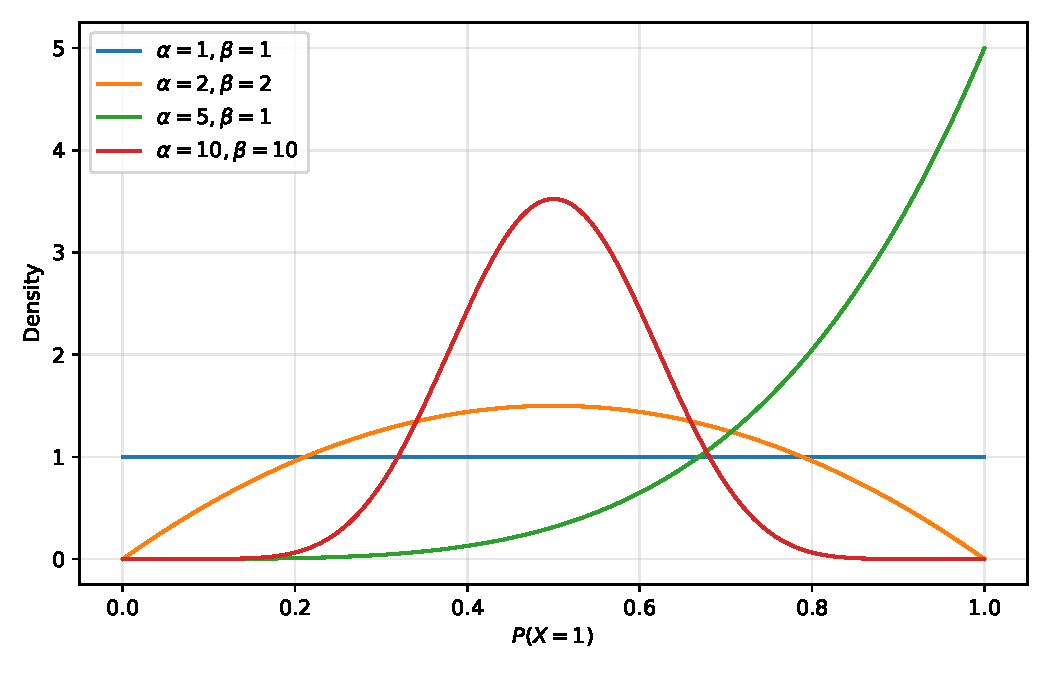
\includegraphics[width=0.65\linewidth]{img/rw/beta_distributions.pdf}
    \caption{Illustration of Beta distributions for different parameter values \((\alpha,\beta)\), showing how second-order uncertainty over \(P(X=1)\) varies from concentrated to highly uncertain.}
    \label{fig:beta_distribution}
\end{figure}

When the variable of interest can take more than two discrete values, the Beta distribution generalizes to the \emph{Dirichlet distribution}. Let \(X\) take values in a finite set \( \{x_1,\dots,x_K\} \), and let \( \mathbf{P} = (P_1,\dots,P_K) \) denote the corresponding probability vector, with \( \sum_{k=1}^{K} P_k = 1 \). Second-order uncertainty over this vector is then modeled by a Dirichlet distribution.

\begin{definition}[Dirichlet Distribution]
\label{def:dir}
A random vector \( \mathbf{P} \in \Delta^{K-1} \) follows a Dirichlet distribution with parameter vector \( \boldsymbol{\alpha} = (\alpha_1,\dots,\alpha_K) \), denoted \( \mathbf{P} \sim \mathrm{Dir}(\boldsymbol{\alpha}) \), if its density is
\[
f(\mathbf{P} \mid \boldsymbol{\alpha}) =
\frac{\Gamma\left(\sum_{k=1}^{K} \alpha_k\right)}{\prod_{k=1}^{K} \Gamma(\alpha_k)}
\prod_{k=1}^{K} P_k^{\alpha_k - 1},
\]
defined over the probability simplex \( \Delta^{K-1} \).
\end{definition}

Similarly to the Beta case, the Dirichlet parameters encode the strength and balance of evidence supporting each outcome. Uniform parameters correspond to maximal uncertainty, while peaked distributions indicate strong confidence in specific probability configurations.

\begin{figure}[t]
    \centering
    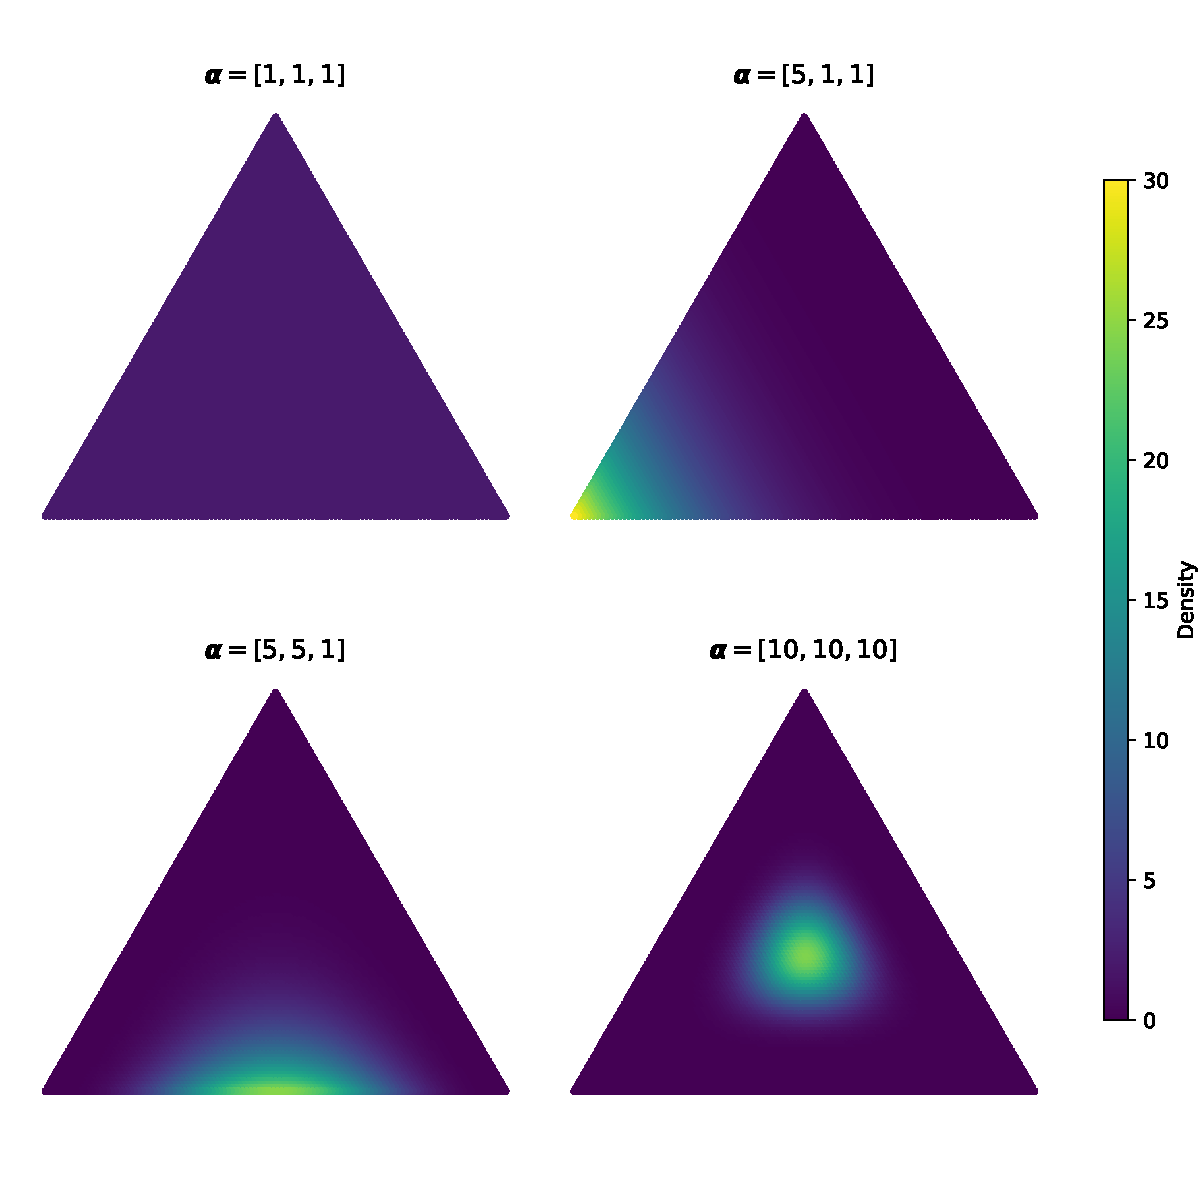
\includegraphics[width=0.65\linewidth]{img/rw/dirichlet_simplex.pdf}
    \caption{Example Dirichlet distributions over a three-class probability simplex, illustrating different degrees of second-order uncertainty.}
    \label{fig:dirichlet_distribution}
\end{figure}

This formulation allows uncertainty arising from missing, incomplete, or ambiguous evidence to be modeled explicitly, instead of being conflated with aleatoric randomness. In contrast to point-valued subjective probabilities, second-order probabilities capture the reliability of a probability assessment, a distinction that has been shown to influence human decision-making under ambiguity \cite{Baron1987}. 

Belief function theory, as introduced by Dempster and Shafer, provides an alternative framework for representing uncertainty under incomplete information. Rather than assigning probability mass exclusively to single events, belief functions distribute mass over sets of hypotheses, allowing part of the belief to remain uncommitted and explicitly representing ignorance. Dempster's rule of combination defines how independent sources of evidence may be fused within this framework. However, Baron shows that belief functions can be interpreted as a \emph{restricted special case} of second-order probability models, corresponding to strong structural constraints on the admissible forms of the distribution \( Q(P) \) \cite{Baron1987}. As a result, belief functions sacrifice expressive generality in exchange for a simplified representation of uncertainty.

This relationship is particularly relevant for uncertainty-aware trust modeling. Second-order probability provides a principled probabilistic foundation for reasoning about uncertainty in probability estimates, while belief-function-based frameworks offer practical tools for aggregating evidence and representing ignorance. These ideas directly inform later developments such as Subjective Logic, which combines second-order uncertainty representation with algebraic operators for trust discounting and fusion.

\subsection{Dempster--Shafer Theory}

\ac{DST}, also known as the theory of belief functions, was introduced to address limitations of classical probabilistic reasoning when evidence is incomplete, imprecise, or conflicting~\cite{shafer1976mathematical,beynon2000dempster}. 
Unlike Bayesian probability theory, which assigns probabilities directly to individual events, \ac{DST} allows belief to be assigned to sets of possibilities, thereby explicitly modeling uncertainty arising from lack of information.

In \ac{DST}, knowledge about a variable is represented through a basic belief assignment (BBA), which distributes belief mass over subsets of the frame of discernment rather than over single outcomes: 
\[
m: 2^{X} \rightarrow [0,1]
\]
It has two properties:
\[
m(\emptyset)=0,
\]
\[
\sum_{A\in 2^{X}} m(A)=1.
\]

This formulation enables a clear distinction between uncertainty due to ignorance and uncertainty due to randomness. In particular, belief mass assigned to composite sets represents epistemic uncertainty, while belief mass assigned to singleton sets reflects support for specific hypotheses.

A central component of \ac{DST} is Dempster’s rule of combination, which provides a mechanism for fusing evidence from multiple independent sources. 
The rule is associative, commutative, and non-idempotent~\cite{josang2012dempster}, which allows evidence to be combined incrementally and without enforcing a fixed aggregation order. 
These properties make \ac{DST} attractive for real-time and distributed applications, such as sensor fusion, where evidence arrives sequentially from multiple sources~\cite{dezert2014on}.

However, the use of Dempster’s rule requires careful consideration. Although the rule is mathematically well-defined, later studies have shown that the combination of highly conflicting sources can lead to counter-intuitive or unstable results~\cite{zadeh2013on,dezert2014on}. In cases of extreme conflict, the normalization step inherent in Dempster’s rule may amplify minor evidence and suppress uncertainty, producing misleading conclusions. As a result, \ac{DST} may become unsuitable when sources strongly disagree or when their reliability differs significantly.

Another limitation of the original \ac{DST} formulation is that it does not explicitly model trust relationships between information sources. All sources are implicitly assumed to be equally reliable, and the theory provides no native mechanism to express trust transitivity or to discount evidence based on the credibility of its origin. This limitation is particularly restrictive in multi-agent systems and distributed environments, where information is often obtained through chains of referrals and where source reliability is heterogeneous.

\subsubsection{Information Fusion and Multi-source Reasoning}
Information fusion aims to combine evidence from multiple sources in order to reduce uncertainty and improve decision quality. This problem arises in a wide range of domains, including sensor fusion, expert systems, and multi-agent systems. In multi-agent settings, agents acquire knowledge through observations or communication, and this knowledge is often represented as beliefs or belief bases~\cite{pigozzi2007aggregation}.

Early work on belief fusion relied primarily on propositional logic-based formalisms~\cite{gregoire2006logic}, and a variety of belief merging operators have been proposed to resolve inconsistencies and aggregate knowledge~\cite{konieczny2002merging,pigozzi2007aggregation,tamargo2012modeling,tran2013axiomatic}. While these approaches provide important theoretical foundations for information aggregation, they typically assume logical consistency or focus on abstract knowledge bases, limiting their applicability to uncertainty-aware reasoning in real-world systems.

\ac{DST} has been widely applied to information fusion in practical systems, particularly in sensor-based applications. For example, Munz and Dietmayer~\cite{munz2011using} employ \ac{DST} to enhance detection performance in sensor fusion systems by explicitly modeling uncertainty and combining sensory evidence. Similarly, Tang et al.~\cite{tang2017improved} use \ac{DST} to represent uncertainty in multi-sensor data before applying evidence fusion.

These works primarily address fusion within a single system, where multiple sensors act as information sources. However, they do not consider trust relationships between independent systems or agents, nor do they address the propagation of trust across information sources. As a result, while \ac{DST} provides a powerful framework for modeling epistemic uncertainty and evidence fusion, it remains limited in its ability to represent source reliability, trust transitivity, and referral-based reasoning.

These limitations motivate extensions of \ac{DST} that explicitly incorporate trust modeling and source dependency. Subjective Logic~\cite{josang2016subjective} builds upon \ac{DST} by introducing subjective opinions, trust discounting, and explicit uncertainty mass, thereby enabling trust reasoning and evidence fusion in distributed and multi-agent environments.

\section{Subjective Logic and Trust}
\ac{SL}~\cite{josang2016subjective,josang2001logic} is a formal framework for reasoning under uncertainty, grounded in probabilistic logic and the \ac{DST} of evidence~\cite{dempster1968generalization,shafer1976mathematical}. 
It extends classical and Bayesian reasoning by explicitly representing uncertainty as a first-class element of its formalism. 
In particular, \ac{SL} enables:
\begin{enumerate}
  \item the explicit representation of uncertainty as part of its fundamental building block, called a \emph{subjective opinion}, and
  \item principled reasoning about uncertainty through \emph{belief fusion}, where multiple subjective opinions are combined using well-defined operators.
\end{enumerate}

\ac{SL} models degrees of beliefs and uncertainty associated with propositions, allowing an agent to express not only what it believes, but also how confident it is in that belief. This makes \ac{SL} particularly suitable for trust modeling and reputation-based systems~\cite{LIU2011547}, as well as for uncertainty-aware assessment of machine learning systems~\cite{sensoy2018evidentialdeeplearningquantify, 10.3389/frai.2020.00054}. By explicitly distinguishing between belief supported by evidence and uncertainty due to lack or conflict of evidence, \ac{SL} addresses limitations identified in probabilistic and Bayesian frameworks.

A core concept of Subjective Logic is the notion of a \emph{subjective opinion}. In the following, we introduce subjective opinions and their formal properties, before presenting the belief fusion and trust discounting operators that enable reasoning and trust propagation in complex systems.


\subsection{Subjective Opinions} 
\label{subsec:SL_opinions}
\begin{figure}
    \centering
    \begin{subfigure}{0.49\textwidth}
    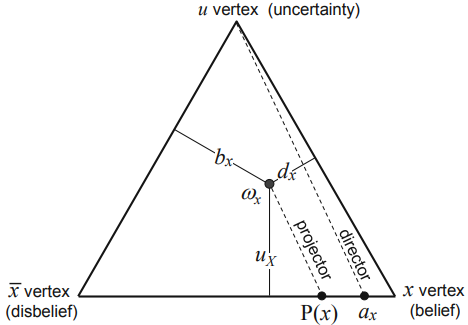
\includegraphics[width=\linewidth]{img/rw/illustration.png}
    \caption{Barycentric triangle visualisation of binomial opinion~\cite{josang2016subjective}.}
    \end{subfigure}
    \begin{subfigure}{0.49\textwidth} 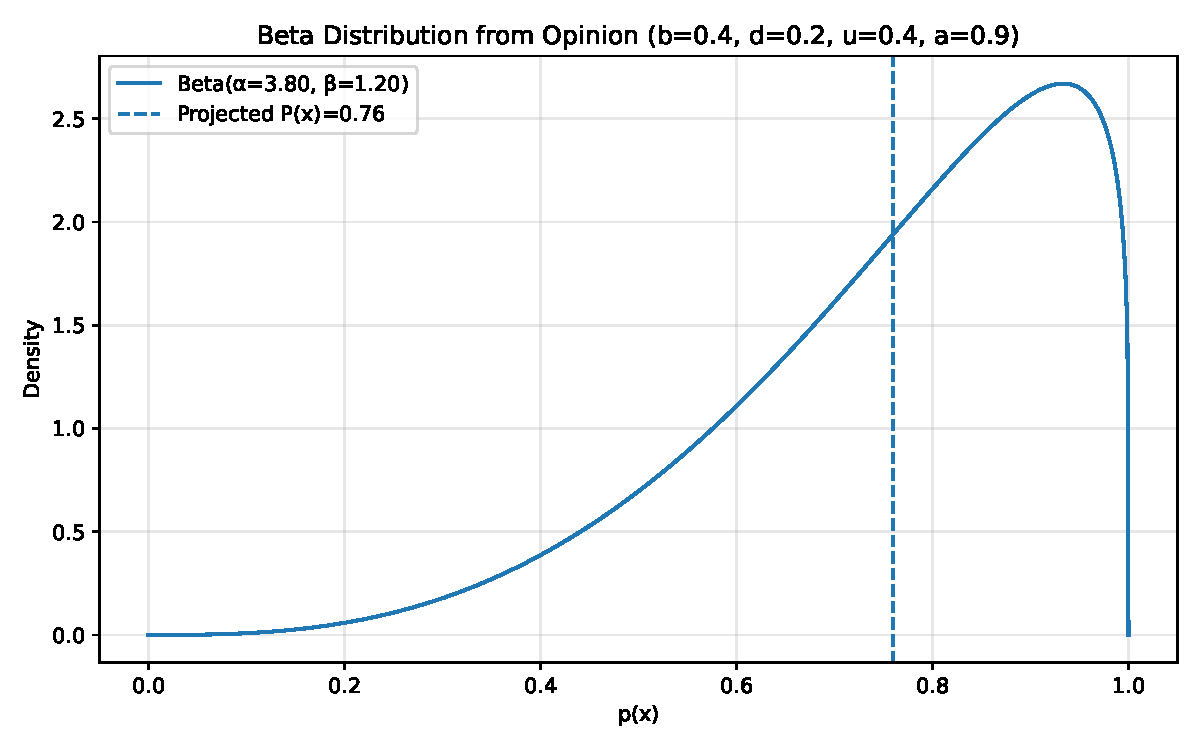
\includegraphics[width=\linewidth]{img/rw/beta_dist_map.pdf}
    \caption{Mapping to a Beta Distribution.}
    \end{subfigure}
    \caption{Binomial Opinion Visualization}
    \label{fig:bin_op_visual}
\end{figure}
Subjective opinions are the fundamental building blocks of Subjective Logic. A subjective opinion represents an agent’s belief about the state of a variable, explicitly capturing both supported belief and residual uncertainty.

Formally, a subjective opinion expresses a belief about a variable $X$ that takes values from a domain $\mathbb{X}$, also referred to as the state space. The domain $\mathbb{X}$ is assumed to be \emph{exhaustive}, meaning that it contains all possible states of $X$, and \emph{exclusive}, meaning that only one state can hold at any given time. Domains may be binary or multi-valued. A binary domain is denoted by $\mathbb{X} = \{x, \overline{x}\}$, where $\overline{x}$ denotes the complement (negation) of $x$.

The notation $\omega_X^A$ denotes a subjective opinion held by agent $A$ about variable $X$. The subscript indicates the target variable or proposition, while the superscript identifies the belief owner. When the belief owner is implicit or irrelevant, the superscript may be omitted for simplicity.

\begin{definition}[Binomial Opinion~\cite{josang2016subjective}] \label{binomial_opinion}
Let $\mathbb{X} = \{x, \overline{x}\}$ be a binary domain with binomial random variable $X \in \mathbb{X}$. 
A binomial subjective opinion about the truth of value $x$ is defined as the ordered quadruplet
\[
\omega_x = (b_x, d_x, u_x, a_x),
\]
where the additivity constraint $b_x + d_x + u_x = 1$ holds, and:
\begin{itemize}
  \item $b_x$ is the belief mass supporting $x$ being true (i.e., $X = x$),
  \item $d_x$ is the disbelief mass supporting $x$ being false (i.e., $X = \overline{x}$),
  \item $u_x$ is the uncertainty mass representing the lack of evidence,
  \item $a_x$ is the base rate, i.e., the prior probability of $x$ in the absence of evidence.
\end{itemize}
\end{definition}

A binomial opinion can be projected onto a probability value using the expected probability operator. The projected probability of $x$ is defined as:
\begin{equation} \label{eq:projected_prob}
	P(x) = b_x + a_x \cdot u_x.
\end{equation}
This projection enables compatibility with classical probabilistic reasoning, while preserving the richer internal representation of belief and uncertainty.


In the context of trust modeling, trust is typically represented as a binomial subjective opinion $(t, d, u)$, where $t$ denotes trust (belief), $d$ denotes distrust (disbelief), and $u$ represents uncertainty. 

\paragraph{Mapping to the Beta Distribution.}

A binomial subjective opinion is bijectively equivalent to a Beta probability density function (PDF). This mapping enables a probabilistic interpretation of belief masses and establishes a bridge between Subjective Logic and Bayesian statistics.

Consider a Beta distribution parameterized by $(\alpha, \beta)$ over the probability variable $p_x \in [0,1]$ (see~\cref{def:beta}) where $\alpha > 0$ and $\beta > 0$ represent evidence supporting $x$ and $\overline{x}$ respectively.

Let $r_x$ and $s_x$ denote positive and negative evidence for $x$. Under the standard non-informative prior weight $W = 2$, the mapping between a binomial opinion 
$\omega_x = (b_x, d_x, u_x, a_x)$ and a Beta distribution is given by:

\begin{equation}
b_x = \frac{r_x}{W + r_x + s_x}, 
\quad
d_x = \frac{s_x}{W + r_x + s_x},
\quad
u_x = \frac{W}{W + r_x + s_x}.
\label{eq:beta_mapping_forward}
\end{equation}

Conversely, for $u_x \neq 0$, the evidence parameters can be recovered as:

\begin{equation}
r_x = \frac{b_x W}{u_x}, 
\quad
s_x = \frac{d_x W}{u_x}.
\label{eq:beta_mapping_inverse}
\end{equation}

The projected probability of the opinion equals the expected value of the Beta distribution:
\begin{equation}
P(x) = b_x + a_x u_x
=
\mathbb{E}[p_x]
=
\frac{\alpha}{\alpha + \beta}.
\end{equation}

This bijective mapping ensures that:
\begin{itemize}
    \item High belief corresponds to concentrated density around high probability values;
    \item High uncertainty corresponds to a flat (uniform) Beta distribution;
    \item A vacuous opinion $(0,0,1,a_x)$ maps to a uniform $\mathrm{Beta}(1,1)$ distribution.
\end{itemize}

The geometric interpretation of binomial opinions is illustrated in ~\cref{fig:bin_op_visual}. The left subfigure shows the barycentric triangle representation, where belief, disbelief, and uncertainty form a 2-simplex. The right subfigure shows the equivalent Beta density, whose expectation corresponds exactly to the projected probability in \cref{eq:projected_prob}.


\begin{definition}[Multinomial Opinion~\cite{josang2016subjective}]
Let $\mathbb{X} = \{x_1, \dots, x_n\}$ be a domain with $n > 2$ mutually exclusive and exhaustive states. A multinomial opinion assigns belief masses $b_{x_i}$ to each state $x_i \in \mathbb{X}$, together with a global uncertainty mass $u$, such that
\[
\sum_{i=1}^{n} b_{x_i} + u = 1,
\]
and is complemented by a base rate distribution over $\mathbb{X}$.
\end{definition}


\begin{definition}[Hypernomial Opinion~\cite{josang2016subjective}]
A hypernomial opinion generalizes multinomial opinions by allowing belief mass to be assigned to subsets of the domain $\mathbb{X}$, enabling representation of partial or composite hypotheses.
\end{definition}

\paragraph{Mapping to the Dirichlet Distribution.}

Multinomial subjective opinions are bijectively equivalent to Dirichlet probability density functions (PDFs). This mapping generalizes the binomial–Beta correspondence and provides a Bayesian interpretation of belief masses as normalized statistical evidence.

Let $\mathbb{X} = \{x_1, \dots, x_k\}$ be a domain of cardinality $k > 2$, and let $\boldsymbol{p} = (p_1, \dots, p_k)$ be a categorical probability vector such that $\sum_{i=1}^{k} p_i = 1$.

The Dirichlet distribution parameterized by the strength vector $\boldsymbol{\alpha} = (\alpha_1, \dots, \alpha_k)$ (see \cref{def:dir}) and the parameters $\alpha_i$ represent accumulated evidence supporting outcome $x_i$.

\paragraph{Evidence Parameterization.}

Let $r_{x_i}$ denote the positive evidence supporting state $x_i$, and let $a_{x_i}$ be the base rate distribution satisfying $\sum_i a_{x_i} = 1$. 
With non-informative prior weight $W$ (typically $W = 2$), the Dirichlet strength parameters are expressed as:

\begin{equation}
\alpha_i = r_{x_i} + a_{x_i} W.
\end{equation}

The expected probability of the Dirichlet distribution is:

\begin{equation}
\mathbb{E}[p_i]
=
\frac{\alpha_i}{\sum_{j=1}^{k} \alpha_j}
=
\frac{r_{x_i} + a_{x_i} W}
{W + \sum_{j=1}^{k} r_{x_j}}.
\end{equation}

\paragraph{Bijective Mapping.}

The multinomial opinion $\omega_X = (\{b_{x_i}\}, u, \{a_{x_i}\})$ is equivalent to a Dirichlet PDF through the following mapping:

\begin{equation}
b_{x_i}
=
\frac{r_{x_i}}
{W + \sum_{j=1}^{k} r_{x_j}},
\qquad
u
=
\frac{W}
{W + \sum_{j=1}^{k} r_{x_j}}.
\label{eq:dirichlet_forward_mapping}
\end{equation}

Conversely, for $u \neq 0$:

\begin{equation}
r_{x_i}
=
\frac{W \, b_{x_i}}{u}.
\label{eq:dirichlet_inverse_mapping}
\end{equation}

Under this bijection, the projected probability of the multinomial opinion

\begin{equation}
P(x_i) = b_{x_i} + a_{x_i} u
\end{equation}

coincides exactly with the expected value of the Dirichlet distribution:

\begin{equation}
P(x_i) = \mathbb{E}[p_i].
\end{equation}

This equality ensures mathematical consistency between subjective opinions and Bayesian probability theory.

To make subjective opinions operational, Subjective Logic provides a set of reasoning operators for combining, revising, and discounting opinions. 
These operators are introduced in the following subsections.


\subsection{Belief Fusion Operators}
Belief fusion operators enable multiple subjective opinions about the same proposition to be combined into a single, aggregated opinion~(\cref{fig:sl_belief_fusion}). 
\begin{figure}[t]
    \centering
    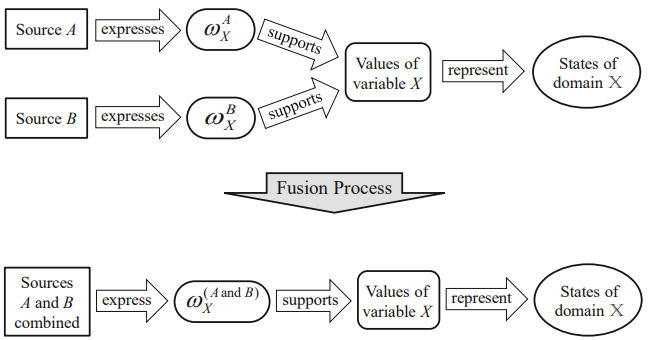
\includegraphics[width=0.6\linewidth]{img/rw/fusion_process.png}
    \caption{Belief fusion process in Subjective Logic. Two sources $A$ and $B$ express subjective opinions $\omega_X^A$ and $\omega_X^B$ about the same variable $X$. The fusion process aggregates these opinions into a single combined opinion $\omega_X^{(A \wedge B)}$, which represents the collective belief over the states of the domain of $X$~\cite{josang2016subjective}.}
    \label{fig:sl_belief_fusion}
\end{figure}

In Subjective Logic, fusion is not governed by a single universal operator; instead, multiple fusion operators are defined, each corresponding to different assumptions about the nature of the evidence sources and the fusion situation~\cite{josang2016subjective,josang2017multi}.

The need for multiple fusion operators arises from the observation that belief sources may differ in important ways, including their independence, reliability, degree of conflict, and the intended semantics of aggregation. Applying an inappropriate fusion operator can lead to misleading or counter-intuitive results. Consequently, scenario with different characteristics might need different fusion operator.

Subjective Logic defines the following principal fusion operators: \emph{constraint fusion}, \emph{cumulative fusion}, \emph{averaging fusion}, \emph{weighted fusion}, and \emph{consensus \& compromise fusion}. Each operator satisfies different algebraic properties, such as idempotence, associativity, and the existence of a neutral element, which reflect the assumptions under which the operator is valid.

\begin{figure}
    \centering
    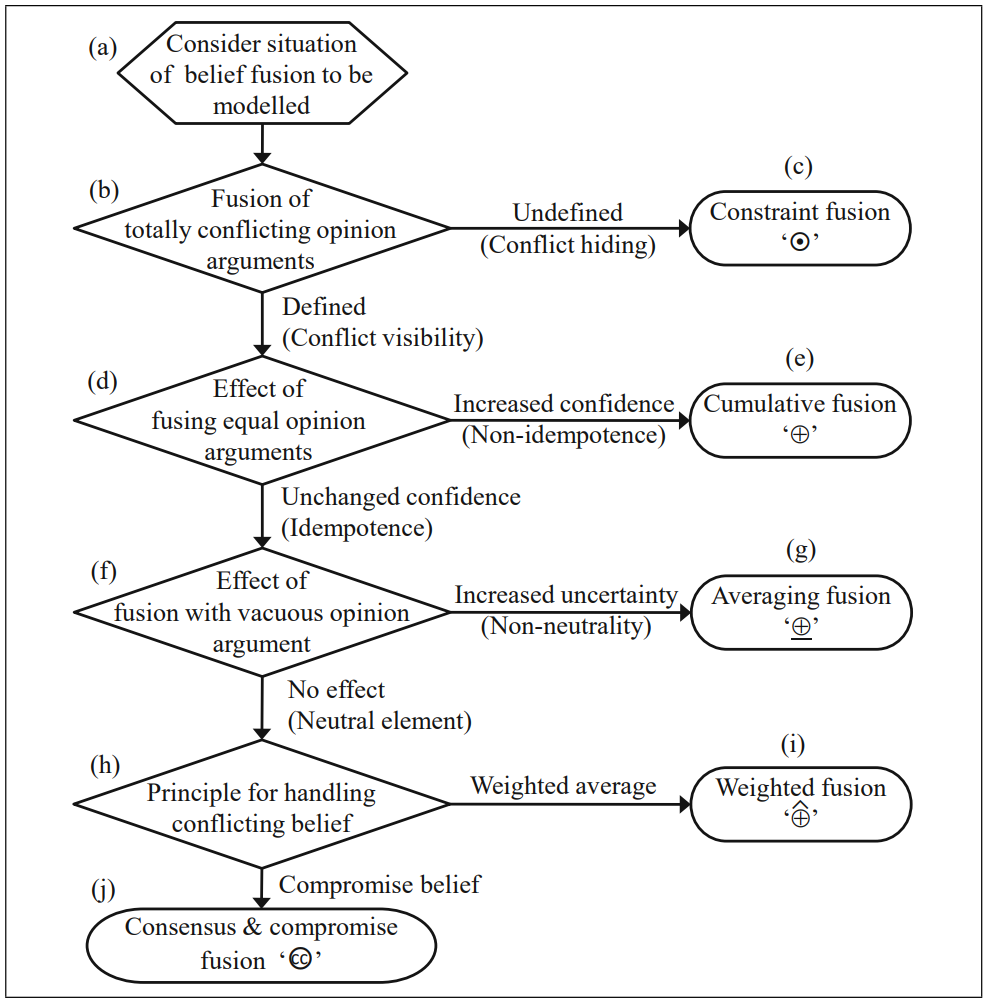
\includegraphics[width=0.65\linewidth]{img/rw/fusion_op_selection.png}
    \caption{Procedure for selecting the most adequate fusion operator}
    \label{fig:sl_fusion_selection}
\end{figure}

J{\o}sang~\cite{josang2016subjective} proposes a structured decision procedure for selecting the most appropriate fusion operator based on a sequence of semantic questions about the fusion situation. This procedure, illustrated in Figure~\ref{fig:sl_fusion_selection}, considers, among others, the following aspects:
\begin{itemize}
    \item whether totally conflicting opinions should result in an undefined outcome or a compromise,
    \item whether repeated identical opinions should increase confidence (non-idempotence) or preserve it (idempotence),
    \item whether vacuous opinions should influence the fusion result,
    \item and how conflicts between belief sources should be resolved.
\end{itemize}


\paragraph{Constraint Fusion}
Constraint fusion is appropriate when opinions are interpreted as hard or soft constraints on the possible states of a variable, and when no compromise is acceptable in the presence of total conflict. In such cases, fusion is undefined if the constraints are mutually exclusive, making conflict explicitly visible rather than hidden. This operator is particularly suitable for preference aggregation and decision-making scenarios.


\paragraph{Cumulative Fusion}
Cumulative fusion assumes that belief sources provide independent evidence about the same phenomenon. 
Under this assumption, fusing additional opinions increases the overall amount of evidence and reduces uncertainty, resulting in a non-idempotent operator. 
Cumulative fusion is commonly applied in sensor fusion and statistical evidence aggregation, where repeated observations strengthen confidence.

\paragraph{Averaging Fusion}
Averaging fusion is designed for situations where belief sources are dependent, such that combining additional opinions does not increase the total amount of evidence. This operator is idempotent and treats all opinions symmetrically, including vacuous ones. It is appropriate when opinions represent different interpretations of the same underlying observations, for example in surveys or jury deliberations.

\paragraph{Weighted Fusion}
Weighted fusion generalises averaging fusion by weighting opinions according to their confidence. More confident opinions exert greater influence on the fused result, while highly uncertain opinions contribute less. This operator is particularly relevant in expert systems, where sources may have unequal expertise or reliability, but where independence cannot be assumed.

\paragraph{Consensus \& Compromise Fusion}
Consensus \& compromise fusion explicitly separates shared belief from conflicting belief. Shared belief is preserved, while conflicting belief is transformed into uncertainty or vague belief, resulting in a compromise that reflects disagreement without artificially favouring one source. 
This operator is especially well suited for fusing hyper-opinions and for situations where preserving epistemic caution in the presence of conflict is essential.

More details about all the operators can be found in~\cref{app:SL_ops}.
\vspace{1em}

In summary, the availability of multiple fusion operators allows the analyst to align the fusion mechanism with the semantics of the application domain. This flexibility is essential for trust reasoning, where inappropriate aggregation of beliefs can lead to overconfidence or misplaced trust. In the next subsection, we introduce trust discounting operators, which explicitly model source reliability and enable trust propagation across networks of agents.


\subsection{Trust Discounting Operators} \label{subsec:TD_operators}
Trust discounting operators are a central component of Subjective Logic, enabling the propagation of trust through intermediary agents. They formalize the intuition that trust in a source should attenuate when information is relayed through other entities, thereby capturing the notion of trust transitivity.

In his foundational work~\cite{josang2016subjective}, J{\o}sang introduces two primary trust discounting operators corresponding to two distinct trust propagation scenarios: \emph{Two-Edge Path} discounting and \emph{Multi-Edge Path} discounting. These operators differ in both their semantic interpretation and their algebraic properties, and they must not be conflated.

\paragraph{Two-Edge Path Trust Discounting}
The Two-Edge Path discounting operator models trust propagation across exactly two adjacent edges: a \emph{referral trust} edge from agent $A$ to agent $B$, and a \emph{functional trust} edge from agent $B$ to a variable $X$. This situation is illustrated in Figure~\ref{fig:tdis}. The resulting discounted opinion represents the belief of $A$ about $X$, derived via its trust in $B$.

\begin{figure}[t]
\centering
    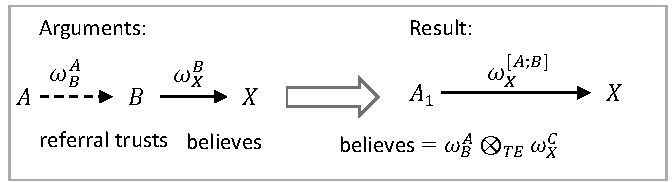
\includegraphics[width=0.7\textwidth]{img/discount/tdis.pdf}
    \caption{Trust discounting for a Two-Edge Path~\cite[Ch.~14.3]{josang2016subjective}}
    \label{fig:tdis}
\end{figure}

Formally, the Two-Edge Path discounting operator $\otimes_{TE}$ is defined as~\cite{josang2016subjective}:
\begin{equation}
    \label{equ:td}
    \omega_X^{[A;B]} = \omega^A_B \otimes_{TE} \omega^B_X =
        \begin{cases}
            b^{[A;B]}_X = P^A_B \, b^B_X,\\
            d^{[A;B]}_X = P^A_B \, d^B_X, \\
            u^{[A;B]}_X = 1 - (b^{[A;B]}_X + d^{[A;B]}_X),\\
            a^{[A;B]}_X = a^B_X,
        \end{cases}
\end{equation}
where $P^A_B$ denotes the projected probability of the referral trust opinion $\omega^A_B$ (cf. Eq.~\ref{eq:projected_prob}). 
This operator corresponds to the \emph{Base Rate Sensitive Transitivity} introduced in~\cite{josang2006exploring}.

\paragraph{Multi-Edge Path Trust Discounting}
In many real-world systems, trust is propagated across longer referral chains involving multiple intermediate agents. The Multi-Edge Path discounting operator generalizes Two-Edge Path discounting to arbitrary-length trust paths, as illustrated in Figure~\ref{fig:tdism}. Consider a trust path from agent $A_1$ to variable $X$ via intermediate agents $A_2, A_3, \dots, A_n$.

\begin{figure}[t]
    \centering
    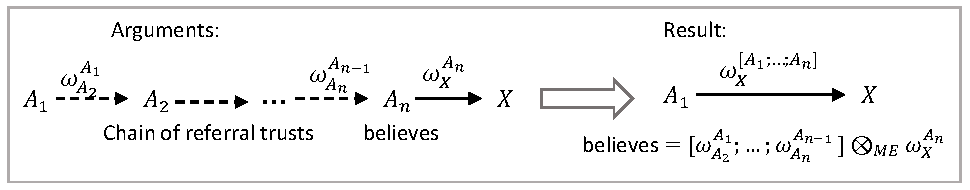
\includegraphics[width=0.8\textwidth]{img/discount/tdisM.pdf}
    \caption{Trust discounting for a Multi-Edge Path~\cite[Ch.~14.3]{josang2016subjective}}
    \label{fig:tdism}
\end{figure}

The resulting discounted opinion $\omega_X^{[A_1;\ldots;A_n]}$ is defined as:
\begin{align}
\label{equ:tdm}
    \omega_X^{[A_1;\ldots;A_n]} &=
    [\omega^{A_1}_{A_2}; \ldots; \omega^{A_{n-1}}_{A_n}] \otimes_{ME} \omega^{A_n}_X
    \\
        &=
        \begin{cases}
            b^{[A_1;\ldots;A_n]}_X = P^{A_1}_{A_n} \, b^{A_n}_X,\\
            d^{[A_1;\ldots;A_n]}_X = P^{A_1}_{A_n} \, d^{A_n}_X,\\
            u^{[A_1;\ldots;A_n]}_X = 1 - (b^{[A_1;\ldots;A_n]}_X + d^{[A_1;\ldots;A_n]}_X),\\
            a^{[A_1;\ldots;A_n]}_X = a^{A_n}_X,
        \end{cases} \notag
\end{align}
where the projected probability of the referral path is computed as
\begin{equation}
\label{equ:proj_prob}
P^{A_1}_{A_n} = \prod_{i=1}^{n-1} P^{A_i}_{A_{i+1}}.
\end{equation}

\paragraph{Discussion}
It is important to emphasize that the Two-Edge Path operator $\otimes_{TE}$ and the Multi-Edge Path operator $\otimes_{ME}$ are distinct operators with different semantics and usage constraints. In particular, both operators require that the final edge in the path corresponds to a functional trust relationship. Table~\ref{table:TD_operators} summarizes the trust discounting operators used in this work.

\begin{table}[t]
\caption{Trust discounting operators}
\centering
\begin{tabular}{|c|c|c|}
\hline
\textbf{Operator} & \textbf{Symbol} & \textbf{Application} \\ \hline
Two-Edge Path & $\otimes_{TE}$ & $\omega^A_B \otimes_{TE} \omega^B_X$ \\ \hline
Multi-Edge Path & $\otimes_{ME}$ & $[\omega^{A_1}_{A_2}; \dots; \omega^{A_{n-1}}_{A_n}] \otimes_{ME} \omega^{A_n}_X$ \\ \hline
\end{tabular}
\label{table:TD_operators}
\end{table}

\paragraph{Limitations}
J{\o}sang et al.~\cite{josang2006exploring} further investigate alternative trust transitivity (trust discounting) operators, including uncertainty-favouring and opposite-belief-favouring transitivity. However, a common limitation of these operators is that trust discounting is applied uniformly across all edges of the trust path. None of the existing operators supports selective discounting restricted to referral edges while preserving functional trust semantics. This limitation prevent to analyze some type of networks where we needs at some point to discount a referral trust opinion with another referral trust opinion. More details about that will be given in the following section, where we will see an example.

\subsection{Subjective Trust Networks} \label{subsec:SL_STN}
% \todo[inline]{Add an example using the one in the trust discounting paper. Then show limitation of current trust discounting operators}
\acp{STN} provide a graph-based formalism for modeling and reasoning about trust relationships using Subjective Logic. In an \ac{STN}, entities such as agents, systems, or sensors are represented as nodes, while directed edges encode trust relationships expressed as subjective opinions.

Formally, an \ac{STN} is represented as a directed graph $G = (V, E)$, where each node $A \in V$ corresponds to an entity, and each directed edge $(A,B) \in E$ is labeled with a binomial opinion $\omega^A_B$, representing the trust of $A$ in $B$ with respect to a given scope or context.Trust relationships may be \emph{referral trust}, expressing confidence in another agent’s reporting ability, or \emph{functional trust}, expressing confidence in the correctness of information about a specific variable.

\paragraph{Trust Inference in \acp{STN}}
To infer trust between nodes that are not directly connected, Subjective Logic relies on the trust discounting and belief fusion operators. Trust discounting is used to propagate trust along directed paths and belief fusion is used to combine multiple opinions about the same target. 

\paragraph{Trust Computation Example: Intersection Movement Assistance}
Intersection Movement Assistance (IMA) is a safety-critical application in \ac{C-ITS}, where vehicles and infrastructure components exchange information to improve road safety, traffic efficiency, and coordination. Consider the IMA scenario illustrated in Figure~\ref{fig:IMA_intersection}. Vehicle $A$ approaches an intersection and communicates via \ac{V2V} communication with vehicles $B$ and $C$. \ac{V2V} communication enables vehicles to exchange information about their state and driving behaviour~\cite{dey2016vehicle}. Vehicles $B$ and $C$ are, in turn, able to communicate with vehicle $D$, which is also approaching the intersection.

\begin{figure}[t]
    \centering
    \begin{subfigure}[b]{0.4\textwidth}
    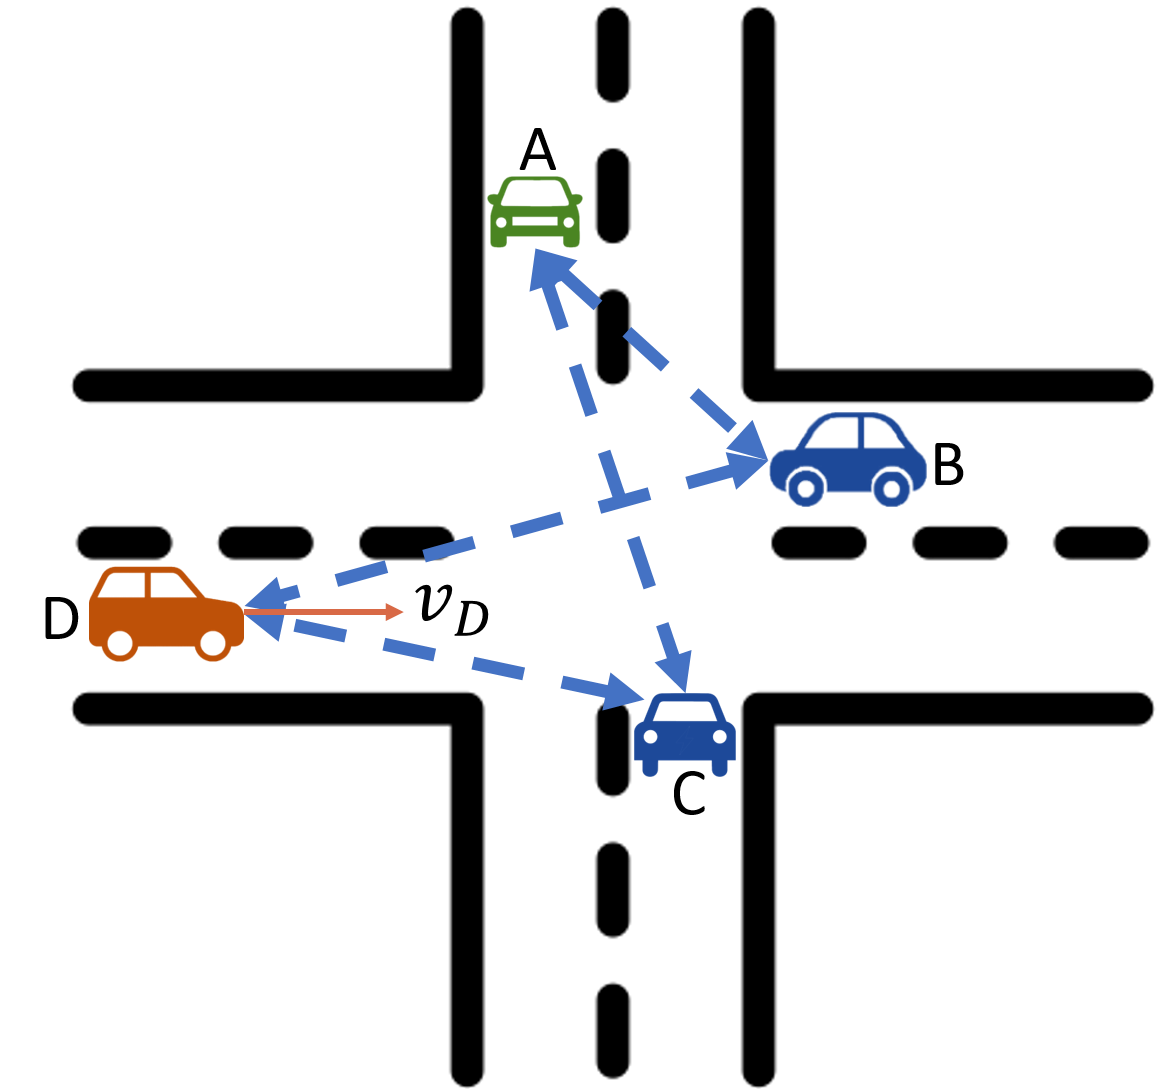
\includegraphics[width=\textwidth]{img/discount/IMA_intersection.png}
    \caption{Intersection Movement Assistance (IMA) \\ scenario}
    \label{fig:IMA_intersection}
    \end{subfigure}
    \begin{subfigure}[b]{0.59\textwidth}
    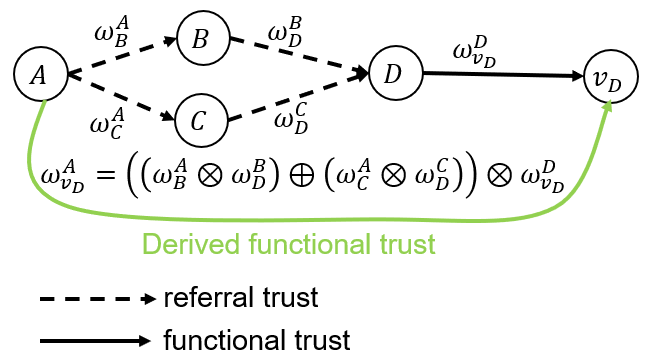
\includegraphics[width=\textwidth]{img/discount/IMA_dissertation.png}
    \caption{IMA example corresponding Subjective Trust Network}
    \label{fig:STN}
    \end{subfigure}
    \caption{}
\end{figure}

In this scenario, vehicle $A$ is interested in assessing the trustworthiness of the velocity information $v_D$ reported for vehicle $D$. Since $A$ cannot directly communicate with $D$, it cannot form a direct trust opinion about $v_D$. Instead, $A$ must rely on indirect evidence obtained through vehicles $B$ and $C$, which act as intermediaries.

This situation can be naturally modeled as a Subjective Trust Network. Vehicle $A$ holds referral trust opinions $\omega^A_B$ and $\omega^A_C$ toward vehicles $B$ and $C$, respectively, reflecting how much $A$ trusts them to provide reliable information. Vehicles $B$ and $C$ each hold functional trust opinions $\omega^B_{v_D}$ and $\omega^C_{v_D}$ regarding the velocity of vehicle $D$.

To derive its own trust opinion about $v_D$, vehicle $A$ first applies trust discounting along each referral path:
\[
\omega^{[A;B]}_{D} = \omega^A_B \otimes\omega^B_{D}, \qquad
\omega^{[A;C]}_{D} = \omega^A_C \otimes\omega^C_{D}.
\]
These discounted opinions represent $A$’s trust in \(D\) via $B$ and $C$, respectively. Since the two paths are independent, the resulting opinions are then fused to obtain a consolidated trust assessment in \(D\):
\[
\omega^A_{D} = \omega^{[A;B]}_{D} \oplus \omega^{[A;C]}_{D},
\]
where $\oplus$ denotes an appropriate belief fusion operator selected based on the semantic assumptions of the application. Finally the trust in the information \(v_D\) is:
\[
\omega^A_{v_D} = \omega^A_{D} \otimes \omega^D_{v_D} = \left( \left( \omega^A_B \otimes\omega^B_{D} \right) \oplus \left( \omega^A_C \otimes\omega^C_{D} \right)  \right) \otimes \omega^D_{v_D}
\]

This example illustrates how Subjective Trust Networks enable principled trust computation in distributed systems. Trust discounting captures the attenuation of trust across intermediaries, while belief fusion aggregates evidence from multiple independent sources. Moreover we can see that \(\omega^A_B\) and \(\omega^B_{D}\) are both referral trust opinion, therefore existing trust discounting operators cannot be used in this case. Improving trust discounting operators is then needed. \ac{SL} mechanism is essential for enabling cooperative decision-making. This motivate the need for structurally sound trust reasoning frameworks, as discussed in the following section.

\paragraph{Structural Constraints and Validity}
Trust reasoning in \acp{STN} relies on repeated applications of discounting and fusion operators along graph paths. However, not all graph structures allow computations using these operators alone. In particular, the correctness and consistency of trust inference are guaranteed when the underlying trust network satisfies the properties of a \ac{DSPG}~\cite{josang2016subjective}.

When an \ac{STN} is not a \ac{DSPG}, trust propagation may lead to ambiguous results, requiring graph transformation or restructuring before trust reasoning can be applied. Ensuring valid trust inference through structural constraints is therefore a central challenge in large-scale trust networks. We'll see more about \ac{DSPG} in the following section.


\subsection{Directed Series--Parallel Graphs (DSPG)}\label{sec:dspg}
\begin{figure}
    \centering
    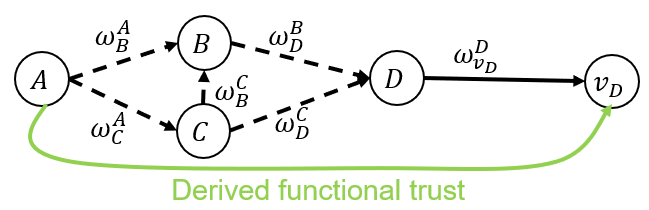
\includegraphics[width=0.5\linewidth]{img/dspg/nonDSPGIMA.png}
    \caption{Example of non DSPG \ac{STN} for the IMA usecase}
    \label{fig:non_DSPG_IMA}
\end{figure}
In \ac{TNA-SL}, \acp{DSPG} constitute the canonical graph structure that guarantees sound and unambiguous trust computation using discounting and fusion operators. As shown in the previous subsection, trust inference in Subjective Trust Networks relies on repeated applications of these operators along graph paths. However, such operations are only well defined when applied to graphs that satisfy specific structural constraints. For example, if we add a new edge from \(B\) to \(C\) (see \cref{fig:non_DSPG_IMA}) in the \ac{STN} for the IMA usecase, it becomes impossible to find the derived functional trust using trust discounting and belief fusion operators. \acp{DSPG} provide exactly the constraints the graph needs to satisfy in order to be processable.

We begin by introducing the notion of a Series--Parallel Graph, which forms the basis for \acp{DSPG}.

\begin{definition}[Series--Parallel Graph]
\label{def:spgraphs}
An SP-graph (Series--Parallel graph) is a graph that can be recursively reduced to a single edge between a source node $s$ and a sink node $t$ using the following two reduction procedures:
\begin{enumerate}[(i)]
    \item \emph{Series reduction}: replace a pair of edges incident to an intermediate node of degree~2 (excluding source and sink) with a single edge.
    \item \emph{Parallel reduction}: replace a pair of parallel edges with a single edge between their common endpoints.
\end{enumerate}
\end{definition}

Figure~\ref{fig:spgraph} illustrates a step-by-step reduction of an SP-graph. The example proceeds through four reduction stages. Reduction~1 applies the series reduction four times; Reduction~2 applies the parallel reduction twice; Reduction~3 again applies series reduction twice; and Reduction~4 applies a final parallel reduction to obtain a single edge. The existence of such a reduction sequence proves that the original graph is an SP-graph.

\begin{figure}[t]
    \centering
    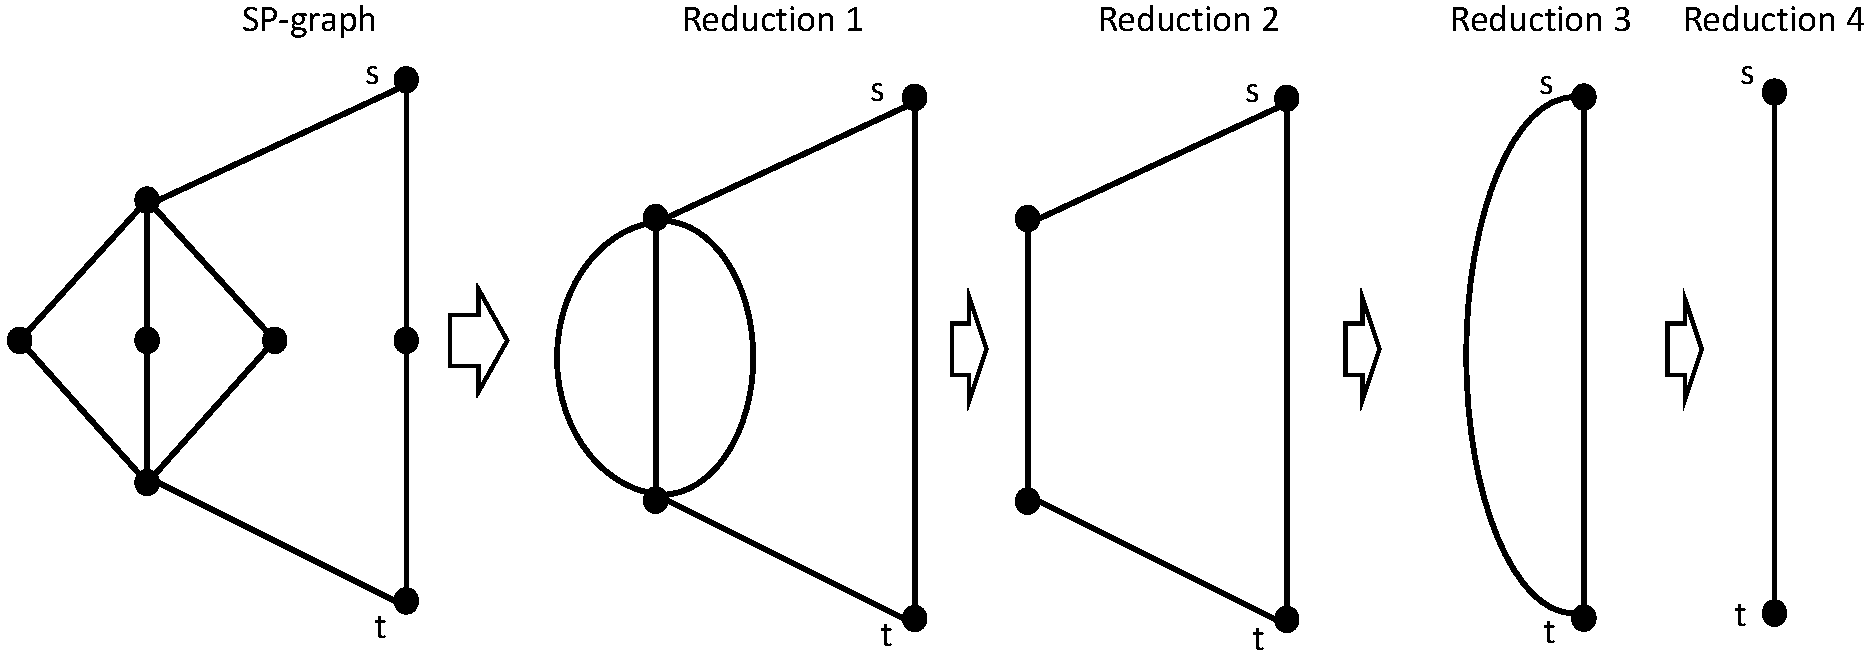
\includegraphics[width=0.6\linewidth]{img/dspg/spgraphs.pdf}
    \caption{Procedure for reducing an SP-graph into a single edge, adapted from~\cite{10.5555/3031657}}
    \label{fig:spgraph}
\end{figure}

An SP-graph that is additionally directed and acyclic, and that contains a unique source and a unique sink, is referred to as a Directed Series--Parallel Graph.

\begin{definition}[Directed Series--Parallel Graph]
A \ac{DSPG} is a directed, acyclic SP-graph composed entirely of directed paths from a unique source node to a unique sink node.
\end{definition}

These properties are essential in the context of trust reasoning. They ensure that trust propagation can be expressed exclusively through well-defined sequences of discounting (along series connections) and fusion (along parallel connections), without ambiguity or operator misuse.

\paragraph{\ac{DSPG} Analysis in Subjective Trust Networks}
In the context of Subjective Trust Networks, \ac{DSPG} analysis refers to the process of computing the derived trust opinion of a source node about a target node or variable using only Subjective Logic discounting and fusion operators. Such a computation is guaranteed to be correct and well defined if and only if the underlying trust network is a DSPG.

To formally capture the structural constraints required for \ac{DSPG} analysis, J{\o}sang introduces the following concepts~\cite{10.5555/3031657}.

\begin{definition}[Parallel Path Subnetwork (PPS)]
\label{def:pps}
A \emph{Parallel Path Subnetwork (PPS)} is a subgraph between two connected nodes $A$ and $B$ such that:
\begin{itemize}
    \item the out-degree of node $A$, denoted $outDegree(A)$, is at least~2, and
    \item the in-degree of node $B$, denoted $inDegree(B)$, is at least~2.
\end{itemize}
\end{definition}

\begin{definition}[Nesting Level (NL)]
\label{def:nl}
The nesting level of an edge in a \ac{DSPG} is defined as the number of Parallel Path Subnetworks (PPSs) to which the edge belongs.
\end{definition}

Figure~\ref{fig:ppsv} illustrates an example \ac{DSPG} and its PPS structure. 
In this example, the PPS list consists of $(A,C)$, $(C,G)$, and $(A,G)$, resulting in an edge nesting level of~2.


\begin{figure}[ht]
        \centering
        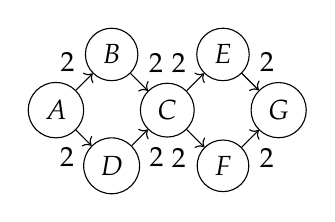
\begin{tikzpicture}[main/.style = {draw, circle}] 
        \node[main] (1) {$A$}; 
        \node[main] (2) [above right of=1] {$B$};
        \node[main] (3) [below right of=1] {$D$}; 
        \node[main] (4) [below right of=2] {$C$};
        \node[main] (5) [above right of=4]{$E$}; 
        \node[main] (6) [below right of=4] {$F$};
        \node[main] (7) [below right of=5] {$G$};
        \draw[->] (1) -- node[midway, above left]{2} (2);
        \draw[->] (1) --  node[midway, below left]{2} (3);
        \draw[->] (2) -- node[midway, above right]{2} (4);
        \draw[->] (3) -- node[midway, below right]{2} (4);
        \draw[->] (4) -- node[midway, above left]{2} (5);
        \draw[->] (4) --  node[midway, below left]{2} (6);
        \draw[->] (5) -- node[midway, above right]{2} (7);
        \draw[->] (6) -- node[midway, below right]{2}  (7);
        \end{tikzpicture}
        \caption{PPS edges NL}
        \label{fig:ppsv}
\end{figure}
Based on these definitions, J{\o}sang proposes an algorithm for computing trust over \acp{DSPG} by iteratively reducing PPSs into single edges while preserving semantic equivalence~\cite[Ch.~15.3]{10.5555/3031657}. At each reduction step, the nesting level is updated accordingly, ensuring that the order of discounting and fusion operations remains consistent with the graph structure.

\begin{figure}
    \centering
    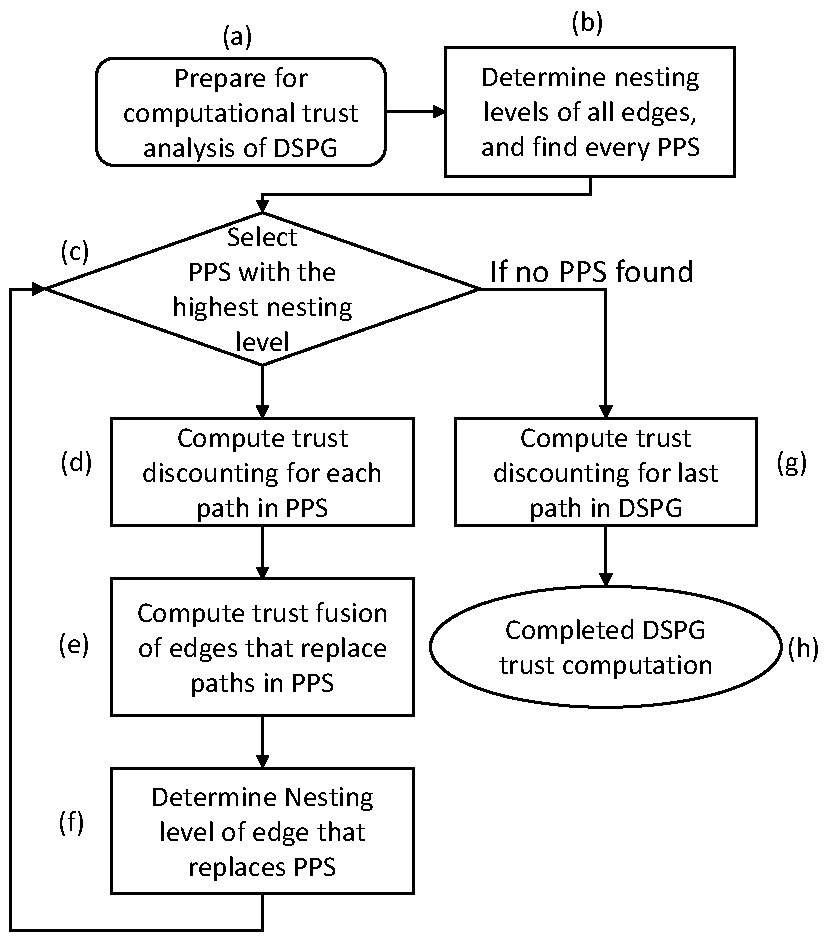
\includegraphics[width=0.5\textwidth]{img/dspg/josangSynth.pdf}
    \caption{Original \ac{DSPG} analysis algorithm by J\o{}sang \cite[Ch.15.3]{10.5555/3031657}}
    \label{fig:algsynth1}
\end{figure}


\section{Trust and Uncertainty in Neural Networks}
\subsection{Neural Networks: Background and Notation}
\label{sec:nn_background}

Neural networks are a class of parametric models widely used for function approximation in machine learning. 
They are composed of multiple layers of interconnected computational units, or neurons, which apply affine transformations followed by nonlinear activation functions. Through layered composition, neural networks can represent complex, high-dimensional mappings and have achieved state-of-the-art performance in a wide range of tasks, including image recognition, natural language processing, and control~\cite{Goodfellow-et-al-2016}.

\paragraph{Network Architecture}
We consider a feedforward neural network parameterized by
\[
\Theta = (\mathbf{W}, \mathbf{b}, f(\cdot)),
\]
where:
\begin{itemize}
    \item $\mathbf{W} = \{\mathbf{W}^{(l)}\}$ is the set of weight matrices, with $\mathbf{W}^{(l)} \in \mathbb{R}^{n_l \times n_{l-1}}$ denoting the weights connecting layer $l-1$ to layer $l$,
    \item $\mathbf{b} = \{\mathbf{b}^{(l)}\}$ is the set of bias vectors, with $\mathbf{b}^{(l)} \in \mathbb{R}^{n_l}$,
    \item $f(\cdot) = \{f^{(l)}(\cdot)\}$ is the set of activation functions, where $f^{(l)}(\cdot)$ denotes the activation applied at layer $l$.
\end{itemize}
Here, $n_l$ denotes the number of neurons in layer $l$, and the network is assumed to consist of $L$ layers.

\paragraph{Feedforward Computation}
Given an input vector $\mathbf{x} \in \mathbb{R}^{n_0}$, the network computes an output $\mathbf{y}' \in \mathbb{R}^{n_L}$ through a sequence of feedforward transformations:
\begin{align}
\label{eq:nnfeed}
\mathbf{y}' &= f_\Theta(\mathbf{x}) \\
\mathbf{y}' &= f^{(L)}\!\left(
\mathbf{W}^{(L)} 
f^{(L-1)}\!\left(
\cdots
f^{(1)}\!\left(
\mathbf{W}^{(1)} \mathbf{x} + \mathbf{b}^{(1)}
\right)
\cdots
\right)
+ \mathbf{b}^{(L)}
\right). \nonumber
\end{align}

This computation can be interpreted as the evaluation of a deterministic computational graph, where each neuron performs a fixed mathematical operation given its inputs and parameters.

\paragraph{Training Objective}
Let $\mathcal{D} = \{(\mathbf{x}_i, \mathbf{y}_i)\}_{i=1}^{N}$ denote a training dataset of input–output pairs. 
Training a neural network consists in optimizing the parameters $\Theta$ to minimize a loss function $\mathcal{L}$ over the dataset:
\[
\Theta^* = \arg\min_{\Theta} \sum_{i=1}^{N} \mathcal{L}\big(f_\Theta(\mathbf{x}_i), \mathbf{y}_i\big).
\]
This optimization is typically performed using variants of gradient descent and backpropagation~\cite{rumelhart1986learning}.

\paragraph{Determinism and Confidence}

Once trained, a standard neural network implements a \emph{deterministic mapping} from inputs to outputs.
Given an input \( x \), the network produces an output vector
\[
\mathbf{o}(x) = g(f_\theta(x)),
\]
where \( f_\theta(x) \) denotes the deterministic computation performed by the network with fixed parameters \( \theta \), and \( g(\cdot) \) is an output transformation chosen according to the task.
In classification settings, \( g \) is commonly selected so that the output components lie in the interval \( [0,1] \) and can be interpreted as class scores or probability-like values.

In practice, these outputs are often treated as estimates of posterior class probabilities,
\[
o_k(x) \approx P(y = k \mid x),
\]
and the predicted class is typically chosen as
\[
\hat{y}(x) = \arg\max_k o_k(x),
\]
with the corresponding maximum value interpreted as the model’s \emph{confidence} in its decision.

However, these confidence values primarily reflect \emph{relative activation strengths} induced by the learned parameters rather than an explicit representation of uncertainty or evidential support.
They arise from deterministic transformations of the input and do not, by themselves, encode information about ambiguity, data scarcity, or model ignorance.

For example, in a binary classification task, output vectors such as \( (0.9, 0.1) \) and \( (0.6, 0.4) \) are commonly interpreted as highly confident and weakly confident predictions, respectively.
Nevertheless, both outputs may result from equally deterministic computations and do not necessarily differ in terms of the quality or reliability of the underlying evidence.

As a consequence, neural networks may assign high confidence to predictions made on \emph{out-of-distribution inputs}, \emph{ambiguous samples}, or data affected by \emph{noise, bias, or corruption}.
In such situations, large output values do not reliably correspond to predictive accuracy or trustworthiness.

This observation highlights a fundamental limitation of confidence estimates derived from standard neural network outputs and motivates the need for \emph{additional mechanisms to quantify uncertainty and assess reliability} beyond raw model confidence, which is the focus of the following section.

\subsection{Uncertainty and Trust Quantification in Neural Networks}
\label{sec:uq_nn}

Quantifying uncertainty in neural networks has become a central research topic, particularly in safety-critical domains such as healthcare, autonomous driving, finance, and industrial automation. In these settings, incorrect yet confident predictions can lead to severe consequences. A representative example is data poisoning, where systematically mislabeled samples are present in both the training and test datasets. In such cases, a model may achieve high accuracy, precision, and recall on the poisoned test set, creating an illusion of reliability despite having learned erroneous or harmful patterns. This highlights a fundamental limitation of standard performance metrics: while they assess predictive accuracy, they fail to capture deeper aspects of predictive reliability and trustworthiness.

Uncertainty Quantification (UQ) seeks to address this limitation by explicitly modeling uncertainty associated with neural network predictions. Rather than producing point estimates alone, UQ methods aim to characterize the full predictive distribution, enabling models to express confidence, ambiguity, and ignorance in a principled manner. Recent surveys provide comprehensive overviews of UQ techniques in deep learning and emphasize their importance for robust and trustworthy AI systems~\cite{Gawlikowski2023,ABDAR2021243}.

In the literature, uncertainty in neural networks is commonly categorized into \emph{aleatoric} and \emph{epistemic} uncertainty~\cite{kendall2017uncertainties,Gawlikowski2023}.

\subsubsection{Aleatoric and Epistemic Uncertainty}

Aleatoric uncertainty captures irreducible uncertainty inherent in the data-generating process, such as sensor noise, measurement errors, or intrinsic variability in observations. This type of uncertainty cannot be reduced by collecting additional data of the same type and is typically modeled as observation noise. Aleatoric uncertainty is often further divided into \emph{homoscedastic} uncertainty, which is constant across inputs, and \emph{heteroscedastic} uncertainty, which varies as a function of the input~\cite{kendall2017uncertainties}.

Epistemic uncertainty, by contrast, arises from limited knowledge about the model parameters or structure. It reflects uncertainty due to insufficient, biased, or unrepresentative training data, as well as uncertainty induced by model misspecification~\cite{neal1996bayesian}. Unlike aleatoric uncertainty, epistemic uncertainty can, in principle, be reduced by acquiring additional data or improving model expressiveness. Figure~\ref{fig:aleatoric_epistemic} provides an illustrative distinction between the two: aleatoric uncertainty manifests as noise around the underlying function, while epistemic uncertainty appears in regions where data are sparse or absent.

This distinction is critical in safety-critical applications. High aleatoric uncertainty may indicate that a task is inherently ambiguous, whereas high epistemic uncertainty suggests that the model is extrapolating beyond its knowledge and that its predictions should be treated with caution.

Beyond this dichotomy, recent work highlights the importance of \emph{distributional uncertainty}, which arises when test samples differ significantly from the training distribution, as in out-of-distribution (OOD) or domain-shift scenarios~\cite{hendrycks2018baselinedetectingmisclassifiedoutofdistribution,ovadia2019trustmodelsuncertaintyevaluating,Gawlikowski2023}. Explicitly modeling distributional uncertainty is essential for detecting unfamiliar inputs and avoiding confident predictions in unsupported regions of the input space.

\subsubsection{Bayesian, Ensemble, and Sampling-Based Approaches}

Foundational approaches to UQ are grounded in Bayesian inference. Bayesian Neural Networks (BNNs) place probability distributions over network parameters and infer posterior distributions given observed data~\cite{neal1996bayesian,blundell2015weightuncertaintyneuralnetworks}. This formulation provides a principled representation of epistemic uncertainty by marginalizing predictions over plausible parameter configurations. However, exact Bayesian inference is computationally intractable for modern deep architectures.

To address this limitation, several approximate inference techniques have been proposed Bayes by Backprop~\cite{blundell2015weightuncertaintyneuralnetworks} employs variational inference to learn approximate posterior distributions over network weights. Monte Carlo dropout interprets dropout at inference time as a variational Bayesian approximation~\cite{gal2016dropoutbayesianapproximationrepresenting}. By performing multiple stochastic forward passes, MC dropout yields predictive distributions that approximate epistemic uncertainty with relatively low computational overhead, and has been widely adopted due to its simplicity.

Deep ensemble methods provide an alternative, non-Bayesian approach to uncertainty estimation~\cite{lakshminarayanan2017simplescalablepredictiveuncertainty}. 
By training multiple models independently and aggregating their predictions, ensembles capture predictive variability and often achieve strong empirical performance in terms of calibration and OOD detection~\cite{ovadia2019trustmodelsuncertaintyevaluating}. However, ensembles are computationally expensive and lack a unified probabilistic interpretation, which complicates the semantic interpretation of their uncertainty estimates.

More structured approaches explicitly model predictive uncertainty using latent variables or hierarchical formulations. For example, latent variable models enable the decomposition of predictive uncertainty into aleatoric and epistemic components~\cite{pmlr-v80-depeweg18a}. These methods have proven particularly useful in active learning and reinforcement learning, where uncertainty-aware decision making can improve sample efficiency and robustness.

\subsubsection{Deterministic and Distributional Uncertainty Methods}

In addition to Bayesian and sampling-based approaches, several deterministic methods aim to estimate uncertainty using a single forward pass.
Softmax confidence scores and predictive entropy are commonly used as simple uncertainty proxies, but they are known to be poorly calibrated and unreliable under distribution shift~\cite{guo2017calibrationmodernneuralnetworks}.

More advanced deterministic methods explicitly model uncertainty at the output level. Prior Networks~\cite{malinin2018predictiveuncertaintyestimationprior} parameterizes Dirichlet distributions over class probabilities, enabling the model to distinguish between data uncertainty and distributional uncertainty. Such methods have shown promise in OOD detection and risk-sensitive classification, although their effectiveness depends strongly on training objectives and data assumptions~\cite{Gawlikowski2023}.

\subsubsection{Calibration and Reliability Challenges}

Despite substantial progress, accurately estimating and calibrating uncertainty in deep neural networks remains challenging. Large-scale empirical studies report frequent over-confidence or under-confidence, particularly under dataset shift, adversarial perturbations, or real-world deployment conditions~\cite{ovadia2019trustmodelsuncertaintyevaluating,begoli2019need}. In medical AI, miscalibrated confidence estimates have been linked to critical decision errors and patient safety risks~\cite{begoli2019need,wolf2025medvlms}.

Calibration refers to the agreement between predicted confidence levels and empirical outcome frequencies. Common evaluation tools include reliability diagrams and scalar metrics such as Expected Calibration Error (ECE) and its variants~\cite{Naeini_Cooper_Hauskrecht_2015}. Post-hoc calibration methods, such as temperature scaling~\cite{guo2017calibrationmodernneuralnetworks}, aim to improve calibration without modifying the underlying model. While effective in many cases, these techniques operate solely at the output layer and do not address uncertainty arising from biased or corrupted training data.


\subsubsection{Uncertainty and Trust Propagation}

Beyond estimating uncertainty at the output level, a growing body of work investigates how uncertainty propagates through neural network architectures and related computational graphs.
The goal of these approaches is to account for the cumulative effect of input uncertainty, parameter uncertainty, and model structure on predictive reliability, while maintaining computational efficiency.

Several methods focus on propagating uncertainty through neural networks without resorting to costly sampling. Mae et~al.~\cite{MAE2021394} proposed a variance propagation framework that converts dropout-trained networks into approximate Bayesian models, enabling uncertainty estimation through analytical propagation of variances. Monchot et~al.~\cite{pmlr-v202-monchot23a} extended uncertainty propagation to non-Gaussian input distributions using Gaussian Mixture Models and a split-and-merge strategy based on the Wasserstein distance, providing theoretical convergence guarantees at reduced computational cost. Earlier work by Astudillo and Net~\cite{astudillo2011propagation} demonstrated that propagating observation uncertainty through multi-layer perceptrons improves robustness in speech recognition systems, including hybrid MLP--HMM architectures.

While these approaches successfully propagate uncertainty through network layers, they primarily focus on statistical uncertainty and do not distinguish between uncertainty arising from data quality, evidence reliability, or trust in information sources. Uncertainty is treated as a numeric attribute that flows through the model, rather than as a semantically meaningful quantity reflecting confidence in evidence.

Outside neural architectures, trust propagation has been extensively studied in networked systems. Ziegler and Lausen~\cite{ziegler2004spreading} proposed the Appleseed model for trust propagation in social networks based on spreading activation. Although not designed for neural systems, this work highlights an important conceptual insight: trust is inherently relational, context-dependent, and shaped by network structure rather than being an intrinsic property of individual nodes.

Taken together, existing uncertainty propagation approaches demonstrate the importance of modeling how uncertainty evolves through computational structures. However, they largely neglect the joint influence of input quality, data reliability, and model parameters on prediction trust. In particular, the trustworthiness of an output cannot be regarded as a fixed property of the model alone; it must depend on the specific input and on how trust and uncertainty propagate through the network’s internal structure.

This observation motivates trust-aware propagation frameworks that treat trust as a dynamic, distributed quantity spanning inputs, parameters, and activations. PaTAS builds on this insight by explicitly modeling trust propagation in alignment with neural network structure, enabling consistent and interpretable reasoning about trust that reflects both data quality and model behavior.

\subsubsection{Limitations with Respect to Trust}

Despite substantial advances in uncertainty quantification and uncertainty propagation, these approaches do not fully address the broader notion of trust in neural networks. Uncertainty quantification primarily captures how unsure a model is about its predictions, but it does not encode whether the underlying evidence is reliable, consistent, or trustworthy.

In particular, UQ methods typically treat uncertainty as a numerical attribute associated with predictions or parameters, without distinguishing between uncertainty caused by irreducible noise, lack of knowledge, or unreliable evidence sources. As a result, uncertainty estimates may remain well-calibrated even when a model is trained on biased, corrupted, or adversarial data, or when predictions are derived from conflicting or low-quality inputs.

Moreover, existing uncertainty propagation techniques focus on how statistical uncertainty flows through network layers, but they do not account for trust relationships between inputs, parameters, or intermediate representations. They lack mechanisms to represent the provenance of information, to discount unreliable components, or to reason about how trust should attenuate or accumulate along computational paths.

This distinction is fundamental. Uncertainty quantification answers the question of \emph{how unsure} a model is, whereas trust assessment addresses \emph{whether the model should be relied upon} in a given context. Trust is inherently relational, context-dependent, and evidence-centric, requiring explicit modeling of source reliability and principled propagation through structured systems.

These limitations motivate trust-aware frameworks that go beyond predictive uncertainty by explicitly modeling evidence quality, trust relationships, and structured propagation. Such frameworks are necessary to support reliable decision-making in safety-critical and high-assurance neural-network applications.


\subsection{Subjective Logic Approaches to Trust in \ac{NN}}

Subjective Logic (SL) provides a probabilistic framework for explicitly modeling belief, disbelief, and epistemic uncertainty, offering a structured and interpretable approach to trust reasoning under incomplete and conflicting evidence. Its explicit separation between belief mass and uncertainty makes SL particularly attractive for trust-sensitive neural network applications, where confidence estimates alone are insufficient to characterize reliability. In recent years, SL has increasingly been adopted to represent predictive uncertainty, aggregate trust from multiple sources, and support structured reasoning about trust across different components of neural systems.

This section reviews existing work that applies Subjective Logic to trust modeling in neural networks. The literature can be broadly grouped into three complementary strands:
\begin{enumerate}[(i)]
    \item opinion-producing neural networks based on evidential learning,
    \item SL-based trust propagation and reasoning within neural or multi-view architectures, and
    \item lifecycle-oriented trust assessment encompassing data, fusion mechanisms, and evaluation metrics.
\end{enumerate}


\subsubsection{Opinion-Producing Neural Networks and Evidential Learning}

The most prominent connection between Subjective Logic and neural networks arises from evidential deep learning (EDL), which leverages the established correspondence between subjective opinions and Dirichlet distributions. In this framework, neural networks output non-negative evidence values that parameterize a Dirichlet distribution, which can be directly mapped to an SL multinomial opinion consisting of belief masses and an explicit uncertainty term~\cite{sensoy2018evidentialdeeplearningquantify}. As a result, the model jointly predicts class probabilities and quantifies epistemic uncertainty in a single forward pass, distinguishing confident predictions supported by strong evidence from uncertain predictions associated with weak or conflicting evidence.

EDL has been widely adopted in multi-view and multimodal learning settings, where uncertainty-aware fusion is essential. Representative examples include trusted multi-view evidential fusion for commonsense reasoning~\cite{yang-2024-trusted}, trusted multi-view learning for long-tailed classification~\cite{tang2025trustedmultiviewlearninglongtailed}, trusted open-world multi-view classification with dynamic opinion aggregation~\cite{10.1145/3746027.3755015} and more~\cite{gao2024comprehensivesurveyevidentialdeep}. In these works, each view produces a subjective opinion, and SL fusion operators are used to aggregate evidence while accounting for view-specific uncertainty. This enables robust decision-making under heterogeneous, noisy, or partially unreliable inputs and provides interpretable uncertainty estimates that guide fusion weights.

However, recent theoretical analyses have raised fundamental concerns regarding the uncertainty semantics of EDL. In particular, Shen et al.~\cite{10.5555/3737916.3741340} demonstrate that many EDL formulations learn spurious epistemic and aleatoric uncertainty: epistemic uncertainty does not vanish with increasing data, and aleatoric uncertainty becomes dependent on model hyperparameters rather than reflecting irreducible data noise. Their analysis shows that common EDL objectives implicitly enforce convergence to a fixed target Dirichlet distribution, causing learned uncertainty to behave more like an energy-based out-of-distribution detector than a faithful uncertainty quantifier. These results indicate that, while EDL is effective for confidence-aware prediction and OOD detection, it does not provide a principled foundation for trust assessment in the presence of biased, corrupted, or strategically manipulated data.

Crucially, evidential approaches implicitly assume that training data and evidence sources are trustworthy. They provide no mechanism to represent uncertainty about data quality, labeling processes, or evidence provenance. Consequently, low uncertainty does not necessarily imply high trust, motivating trust frameworks that operate beyond predictive uncertainty alone.

\subsubsection{Trust Propagation and Reasoning within Neural Architectures}

Beyond opinion-producing outputs, several approaches employ Subjective Logic as an internal reasoning mechanism to propagate trust through neural or multi-component systems. In this line of work, trust is treated as a first-class quantity associated with inputs, views, datasets, or system components, rather than being inferred solely from final predictions.

In multi-view learning, SL operators are frequently used to discount unreliable views and fuse consistent evidence. Dynamic opinion aggregation strategies adjust fusion weights based on uncertainty or conflict, enabling robust reasoning in open-world and long-tailed scenarios~\cite{ZUO2026129453,10.1145/3746027.3755015}. These approaches demonstrate the practical utility of SL fusion semantics, particularly in environments where views differ in reliability or may contradict one another.

A notable white-box attempt is the DeepTrust framework proposed by Cheng et al.~\cite{10.3389/frai.2020.00054}, which integrates dataset-level evidence into a global trust assessment for neural networks. While conceptually appealing, DeepTrust raises theoretical concerns. Specifically, it equates neural-network arithmetic operations with SL fusion and opinion multiplication, despite these operators belonging to different algebraic domains. Fusion combines independent opinions about the same proposition, whereas opinion multiplication combines beliefs over independent propositions; their interchangeability is not formally justified. Moreover, trust backpropagation is defined only at a single-layer level, leaving its extension to deep architectures theoretically unclear.

Overall, existing SL-based trust propagation approaches demonstrate the expressive power of SL but lack a principled alignment with neural network computation graphs and parameter hierarchies.

\subsubsection{Lifecycle-Oriented Trust Assessment: Data, Fusion, and Metrics}

A third strand of research applies Subjective Logic to trust assessment across the broader machine learning lifecycle. Rather than focusing solely on predictions, these approaches model trust in datasets, fusion mechanisms, and evaluation metrics.

At the data level, SL has been used to quantify annotator reliability, labeling uncertainty, and dataset quality, particularly in multi-source or weakly supervised settings. Opinions derived from inter-annotator agreement, sampling variability, or bias indicators allow dataset trustworthiness to be explicitly represented with uncertainty, reinforcing the principle that trust in a neural network is inseparable from trust in its training data.

At the evaluation level, Herd and Burton~\cite{10.1145/3605098.3635966} demonstrate that standard ML performance metrics systematically overestimate safety-relevant performance when treated as point estimates. They propose modeling metrics such as accuracy or recall as subjective opinions derived from binomial evidence, enabling uncertainty-aware safety arguments and trust propagation across assurance layers. This work highlights that trust must be reasoned about not only at prediction time, but also at evaluation and certification stages.

\paragraph{Summary}
Overall, Subjective Logic provides a coherent and expressive framework for modeling trust in neural networks, encompassing predictive uncertainty, multi-source fusion, trust propagation, and lifecycle-wide assessment. Existing work demonstrates the practical benefits of SL-based reasoning, particularly in multi-view and safety-critical settings. At the same time, significant gaps remain. Current approaches often conflate uncertainty with trust, assume trustworthy data, or lack algebraic consistency with neural network structures. These limitations motivate the development of SL-based trust frameworks that explicitly distinguish evidence quality from uncertainty, support principled trust propagation, and align structurally with neural network inference and training processes.


\subsection{Trust and Uncertainty Propagation}
Recent work on uncertainty propagation seeks to improve both accuracy and computational efficiency. Mae et~al.~\cite{MAE2021394} proposed a sampling-free conversion of dropout-trained networks into Bayesian models using variance propagation. Monchot et~al.~\cite{pmlr-v202-monchot23a} employed Gaussian Mixture Models and a Split-and-Merge algorithm with a Wasserstein criterion to propagate input uncertainty without assuming Gaussianity, achieving convergence guarantees at low cost. Astudillo and Net~\cite{astudillo2011propagation} extended these ideas to multi-layer perceptrons for speech recognition, showing that observation uncertainty enhances robustness even in hybrid MLP-HMM systems.

Beyond neural architectures, Ziegler and Lausen~\cite{ziegler2004spreading} proposed the Appleseed model for trust propagation in social networks using dynamic spreading activation. Though not originally intended for neural systems, it demonstrates the value of viewing trust as a structural, context-dependent quantity, an idea further developed in PaTAS.

Existing approaches demonstrate growing interest in uncertainty and trust modeling to assess trust in neural networks, yet they often neglect the joint influence of input quality, data reliability, and model parameters on prediction trust. The trustworthiness of an output cannot be viewed as a fixed property of the model alone but must depend on the corresponding input and its propagation through the network. PaTAS addresses these gaps by modeling trust as a dynamic property distributed across inputs, parameters, and activations, enabling consistent and interpretable trust propagation that reflects both data quality and network structure.


\subsection{AI Attacks and Deception in the AI Lifecycle}
\label{subsec:ai_attacks}

Modern AI systems are exposed to a wide range of adversarial threats that target different stages of the AI lifecycle, from data acquisition to deployment and operation. Unlike traditional software, machine-learning systems derive their behavior from data, making them particularly vulnerable to attacks that exploit data quality, training dynamics, or model behavior rather than code-level vulnerabilities. Figure~\ref{fig:attacks} illustrates a representative AI development pipeline and highlights the broad attack surface spanning data collection, dataset preparation, model training, and inference-time operation.

\begin{figure}[t]
    \centering
    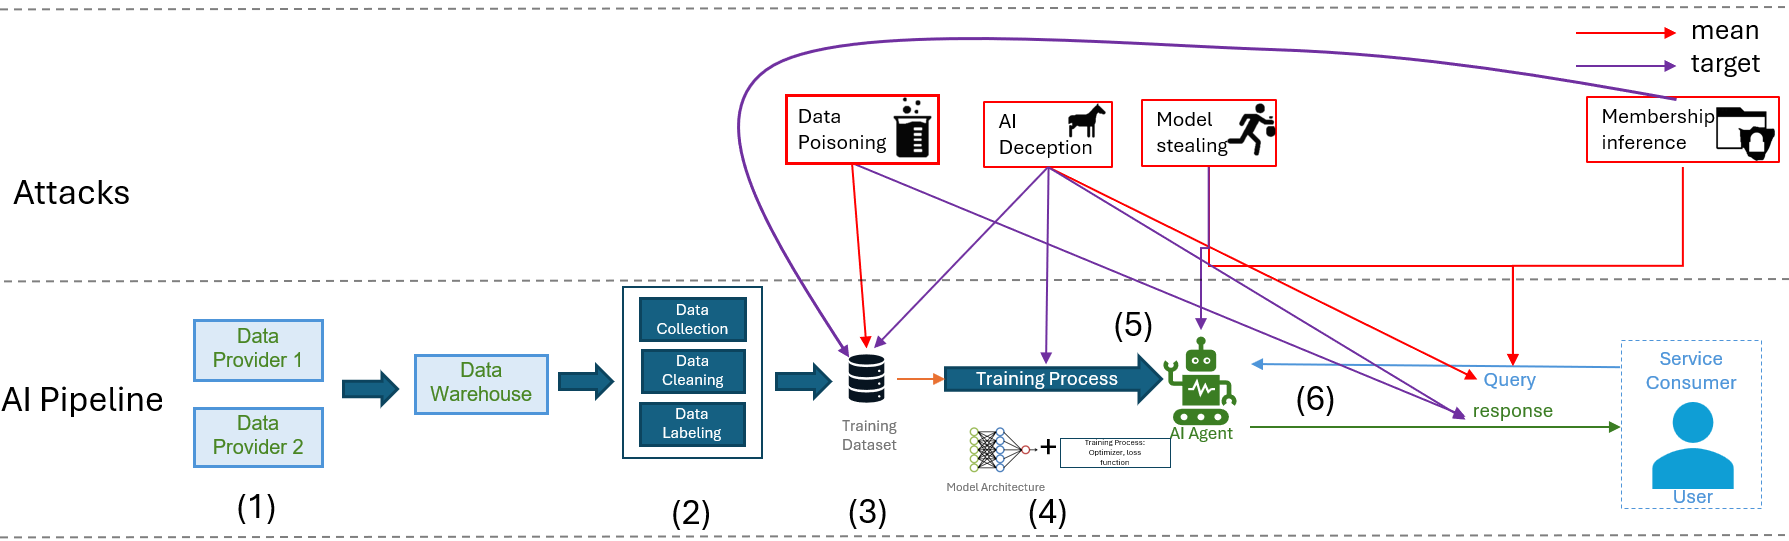
\includegraphics[width=\linewidth]{img/patas/attacks.png}
    \caption{Attack surface in the AI lifecycle pipeline, from data collection to model deployment.}
    \label{fig:attacks}
\end{figure}

\paragraph{Data Poisoning and Training-Time Attacks}
One of the most extensively studied threats is data poisoning, in which adversaries inject malicious or carefully crafted samples into the training dataset~\cite{chen2017targetedbackdoorattacksdeep}. Poisoned data may be mislabeled, backdoored, or statistically biased, causing the trained model to behave incorrectly under specific conditions while maintaining high performance on standard test sets. Such attacks are particularly dangerous because they undermine the assumption that training data faithfully represent the task domain. Standard performance metrics often fail to reveal poisoning effects, allowing compromised models to appear reliable.

\paragraph{Inference-Time Attacks and Model Exploitation}
Beyond training-time manipulation, deployed models are vulnerable to inference-time attacks. Model stealing or extraction attacks exploit repeated queries to reconstruct an approximation of the target model, threatening intellectual property and enabling subsequent adversarial attacks. Membership inference attacks aim to determine whether specific data points were part of the training dataset, raising serious privacy concerns. These attacks exploit overly confident predictions or memorization effects and demonstrate that model outputs can leak sensitive information even in the absence of explicit access to training data.

\paragraph{AI Deception and Strategic Manipulation}
More recently, attention has shifted toward AI deception, where adversarial agents deliberately manipulate inputs, interactions, or contextual information to induce misleading but seemingly plausible model outputs. Unlike classical adversarial examples, deceptive behaviors may not rely on imperceptible perturbations but instead exploit semantic ambiguity, contextual manipulation, or systematic bias in data sources. In multi-agent or human–AI interaction settings, deception may arise from untrusted information sources, colluding agents, or strategically misleading inputs designed to influence downstream decisions without triggering conventional anomaly detection mechanisms.

AI deception highlights a fundamental limitation of confidence-based reliability measures: a system may produce confident, well-calibrated predictions while being systematically misled. Detecting such behaviors requires reasoning not only about uncertainty, but also about the trustworthiness of evidence sources and the propagation of trust through the system.

\paragraph{Trust as a Lifecycle-Wide Concern}
Taken together, these attack classes illustrate that vulnerabilities in AI systems are not confined to a single stage of development. Trust can be compromised during data collection, labeling, training, evaluation, or deployment, and adversarial behavior may manifest long after a model has been trained. Consequently, the trustworthiness of a prediction cannot be viewed as a static property of a model alone, but must be understood as a dynamic property that depends on the provenance, quality, and interaction of data, model parameters, and operational context.

These observations motivate trust-aware frameworks that assess and propagate trust across the AI lifecycle, rather than relying solely on predictive accuracy or uncertainty estimates. Such frameworks aim to complement existing defenses by providing structured, evidence-centric reasoning about reliability and misuse, forming the foundation for the trust assessment approaches discussed in the subsequent sections.

\subsection{Training Dataset Quality and Trustworthiness}
\label{subsec:dataset_quality}

The quality and reliability of training datasets play a central role in determining the trustworthiness of neural network models. Since modern learning systems derive their behavior primarily from data rather than explicit rules, deficiencies in dataset construction can directly translate into systematic model failures. In safety-critical and high-assurance settings, dataset quality must therefore be treated as a first-class concern rather than an implicit assumption.

\paragraph{Data Poisoning and Dataset Trust}
One of the most direct threats to dataset trustworthiness is data poisoning, in which adversaries inject malicious, mislabeled, or carefully crafted samples into the training data. Poisoning attacks can subtly manipulate model behavior, for example by inducing targeted misclassifications or embedding backdoors, while preserving high accuracy on standard test sets. This makes poisoning particularly difficult to detect using conventional performance metrics and highlights a fundamental challenge: high predictive accuracy does not imply that the underlying training data are trustworthy.

More broadly, data poisoning illustrates that dataset trustworthiness is not a binary property but a matter of degree, dependent on the quality, provenance, and consistency of available evidence. Assessing dataset trust therefore requires reasoning under epistemic uncertainty, especially when dataset construction processes are opaque, distributed, or partially adversarial.

\paragraph{Ambiguity, Bias, and Epistemic Uncertainty in Datasets}
Beyond explicit attacks, even benign datasets may suffer from ambiguity, bias, and incomplete documentation. Meyer et al.~\cite{meyer2023multiplicity} emphasize that a single dataset can often support multiple valid interpretations of what it represents, due to unclear population coverage, subjective annotation choices, or undocumented filtering decisions. This multiplicity reveals an often-overlooked source of epistemic uncertainty in dataset evaluation: uncertainty about what claims a dataset actually supports.

Traditional approaches to dataset bias focus on statistical imbalance, demographic parity, or fairness metrics, often using resampling or reweighting techniques~\cite{10.1145/3600211.3604691,roy2022multi}. While effective for certain bias patterns, these methods typically assume that datasets are clean, fully labeled, and centrally accessible. In federated and decentralized learning settings, bias assessment becomes substantially more complex due to client heterogeneity, partition skew, limited metadata, and partial observability~\cite{roy2024fairness,electronics13234664}. Although mitigation strategies such as weighted aggregation or loss regularization have been proposed~\cite{electronics13234664}, existing work rarely quantifies confidence in the bias assessment itself when evidence is incomplete or noisy.

\paragraph{Dataset Evaluation Frameworks and Composite Trust Scores}
To improve transparency and accountability, several frameworks have been proposed to systematize dataset evaluation. Datasheets for Datasets~\cite{gebru2018datasheets} promote structured documentation of data collection, intended use, and known limitations. More recent scorecard-based approaches, such as METRIC~\cite{schwabe2024metric} and FRIES~\cite{10.1007/978-3-031-63787-2_15}, aggregate expert assessments across multiple quality dimensions, including fairness, robustness, and safety.

While these frameworks represent important progress, they largely rely on deterministic expert judgments and assume the availability of complete and reliable metadata. They do not provide formal mechanisms to represent uncertainty, disagreement, or missing evidence, nor do they distinguish between a low trust score and low confidence in the assessment itself. As a result, confidence in dataset evaluation cannot be explicitly reasoned about or propagated.

\paragraph{Annotation Noise and Trust in Labels}
Annotation quality is a critical component of dataset trustworthiness, particularly in supervised learning. Inter-annotator agreement metrics such as Cohen’s Kappa are commonly used to summarize labeling consistency, but these metrics provide only coarse, global measures and obscure instance-level uncertainty.

A substantial body of work on crowd annotation modeling addresses noisy labels by inferring latent ground truth. The seminal Dawid--Skene model~\cite{dawid1979maximum} estimates annotator-specific confusion matrices using expectation--maximization. Subsequent extensions such as GLAD~\cite{whitehill2009whose} incorporate annotator expertise and item difficulty, while MACE~\cite{hovy2013learning} focuses on identifying unreliable or adversarial annotators. Although effective for label denoising, these approaches ultimately collapse disagreement into point estimates of labels or annotator competence, discarding residual uncertainty.

More recent work has applied Subjective Logic to preserve and reason about annotation uncertainty. Subjective Logic Encodings (SLEs)~\cite{SLencodings,vasilakes2025sle} represent inter-annotator disagreement as belief--disbelief--uncertainty triplets, enabling instance-level trust assessment that explicitly distinguishes consensus from ignorance. This perspective aligns with the view that annotation disagreement is not merely noise to be eliminated, but evidence to be interpreted.

\paragraph{Toward Uncertainty-Aware, Data-Centric Trust Assessment}
Subjective Logic has also been applied more broadly to trust assessment in AI systems, including model-level trust~\cite{wang2020there}, evaluation metrics~\cite{10.1145/3605098.3635966}. However, most existing approaches remain model-centric or metric-centric and do not address dataset-level properties such as representativeness, bias, or sampling quality in a unified manner.

Taken together, existing approaches to dataset quality assessment either emphasize qualitative documentation without formal uncertainty modeling, deterministic composite scores without confidence representation, or trust modeling applied to isolated components of the data pipeline. What remains missing is a unified framework that integrates heterogeneous evidence, annotation reliability, bias assessment, and explicit uncertainty reasoning into a coherent evaluation of dataset trustworthiness. Addressing this gap is essential for trustworthy neural-network training and motivates the data-centric trust modeling approaches developed in this thesis.


\section{Synthesis and Gap Summary}
\todo[inline]{Estimated Nb Pages: 1}
% \part{Methodology, Analysis, Implementation, and Results}
% \chapter*{Enhances Trust Analysis with Subjective Logic}
% \label{part:tnasl}
% \addcontentsline{toc}{chapter}{Enhances Trust Analysis with Subjective Logic}
% \chapter{On Subjective Logic Trust Discount for Referral Paths}
\label{chap:ref}

% \chapter*{Assessing Neural Network Trustworthiness}
% \label{part:nntrust}
% \addcontentsline{toc}{chapter}{Assessing Neural Network Trustworthiness}



\chapter{General Trust Assessment Methodology  [By End of March] }
\label{chap:Trust_method}
\section{Role of the General Trust Assessment Methodology}
\label{sec:ch4_role}
This chapter introduces the \emph{General Trust Assessment Methodology} that serves as the conceptual backbone of this dissertation. The methodology is grounded in the Evidence-based \ac{TAF}, originally developed in the context of multi-agent systems within the Horizon Europe CONNECT project~\cite{connect_d31_taf}and also discussed in the 5GAA white paper on trust evaluation~\cite{5gaa_trust_whitepaper}. In this framework, trust is not assumed or statically assigned
but instead derived through a structured reasoning process that includes the generation of expressions, the collection of evidence, and the evaluation of these expressions.

The objective of this chapter is to abstract and generalize this evidence-based reasoning process so that it can be instantiated across different \ac{AI} contexts. While the technical mechanisms used to compute trust may vary across systems, the underlying reasoning process remains largely invariant. The methodology introduced here therefore provides a unified framework for structuring trust assessment problems and systematically deriving trust evaluations from observable evidence.

In the remainder of this dissertation, this general methodology will be instantiated in several distinct settings:

\begin{itemize}
    \item the trust assessment of neural network prediction calibration (\cref{chap:bb}),
    \item the evaluation of training dataset trustworthiness (\cref{chap:data}),
    \item the propagation of trust through neural network architectures using the PaTAS framework (\cref{chap:ptas}).
\end{itemize}

Although these application domains differ in their technical implementations, they share a common conceptual structure. In each case, a \emph{trustor} seeks to determine whether a specific trust proposition holds for a given entity or process, based on available evidence and within a particular contextual setting. The methodology presented in this chapter formalizes this common reasoning structure. In particular, it defines the sequence of steps required to construct a trust assessment and provides guidance on how each step can be operationalized in practice.

The methodology should therefore be understood as a generic trust reasoning engine. Subsequent chapters specialize this engine to particular trustworthiness properties and application domains, while preserving the same conceptual pipeline defined in this chapter.

\section{Core Concepts and Notation}
\label{sec:ch4_core_concepts}
The terminology follows the principles of the \ac{TAF}, which adopts \acf{SL} as the formal reasoning framework for representing and propagating trust. The notation introduced here is therefore consistent with \ac{SL} representations.

% \subsection{Trustor, Trustee, and Trust Proposition}

Trust assessment is inherently relational. A trust evaluation is always performed from the perspective of a \emph{trustor} with respect to a well-defined \emph{trust proposition} encoding a specific \emph{trustee}.

\begin{definition}[Trust Proposition]
A trust proposition is a declarative statement about a property of a trustee
that can be evaluated as satisfied or not satisfied based on available
evidence.
\end{definition}

Formally, let $E$ denotes the trustee and $P$ a
trustworthiness property of interest, such as accuracy, integrity, representativeness, or calibration. The trust proposition is denoted by
\[
\mathcal{T}(E, P)
\]
and represents the statement: ``Entity $E$ satisfies property $P$''

Trust propositions may take different forms:
\begin{itemize}
    \item \textbf{Simple}, when they refer to a single assessable property.
    \item \textbf{Composite}, when they are constructed as logical combinations
    of several simple propositions.
\end{itemize}

Composite trust propositions are typically expressed using logical operators such as conjunction, disjunction, and negation. For example, a composite proposition may take the form

\[
\mathcal{T} = \mathcal{T}_1 \wedge \mathcal{T}_2
\]

where each $T_i$ represents independent simple proposition.



% Each of these properties can be evaluated using separate evidence sources
% before being combined to assess the overall trust proposition.

% \subsection{\acf{ATL}}


% \subsection{Trust Sources and Evidence}


\begin{definition}[\aclu{ATO}]
An \acf{ATO} is a trust opinion associated with a simple trust proposition for which the trustor can directly observe or collect evidence about the trustee. In this case, the trustor maintains a direct evidential relationship
with the trustee and can therefore quantify trust based on observable
evidence.
\end{definition}
In the methodology, trust assessment of \ac{ATO} relies on evidence collected from \emph{trust sources}.

\begin{definition}[Trust Source]
A trust source is any entity, mechanism, or process that provides evidence
relevant to the evaluation of a trust proposition.
\end{definition}

Trust sources may include:

\begin{itemize}
    \item direct observations performed by the trustor,
    \item measurements from sensors or monitoring systems,
    \item reports or certifications provided by third parties,
    \item historical performance records,
    \item reputation information,
    \item outputs of analytical or verification mechanisms.
\end{itemize}


The outcome of the overall process is referred to as the \emph{\acf{ATL}}.
\begin{definition}[\aclu{ATL}]
The \ac{ATL} is the quantified trust opinion assigned by the trustor to a
trust proposition based on the available evidence and the selected evaluation
formalism.
\end{definition}

In this dissertation, the \ac{ATL} is represented using a subjective binomial
opinion:

\[
\omega = (t, d, u)
\]

where $t$ denotes the trust mass (belief of the binomial opinion), $d$ denotes distrust (disbelief of the binomial opinion), and $u$ represents uncertainty. This representation allows the trust assessment to capture not only whether the trustor should trust the proposition, but also the degree of confidence associated with that assessment.

For clarity, the main elements introduced in this section are summarized in \cref{tab:trust_notation}.

\begin{table}[h]
\centering
\begin{tabular}{ll}
\toprule
Symbol & Description \\
\midrule
$A$ & Trustor (entity performing the trust assessment) \\
$E$ & Trustee (entity whose property is being evaluated) \\
$P$ & Trustworthiness property \\
$\mathcal{T}(E,P)$ & Trust proposition stating that entity $E$ satisfies property $P$ \\
$\omega=(t,d,u)$ & trust opinion with belief $b$, disbelief $d$, and uncertainty $u$ \\
\ac{ATO} & \aclu{ATO} associated with a simple proposition \\ 
\ac{ATL} & outcome of the assessment\\
\bottomrule
\end{tabular}
\caption{Notation used in the general trust assessment methodology.}
\label{tab:trust_notation}
\end{table}

These concepts provide the conceptual foundation for the trust assessment process introduced in the next section.

\section{The Trust Assessment Process}
\label{sec:ch4_three_phase}

Having introduced the core concepts and notation, we now present the
general trust assessment process. This process follows the \ac{TAF} methodology and consists of three sequential phases:

\begin{enumerate}
    \item Expression Generation that sometimes necessitate a \ac{STN}. The expression consists in operations between \acp{ATO}.
    \item \acp{ATO} Quantification
    \begin{enumerate}
        \item Identify trust sources and Collect Evidence for each proposition
        \item Quantify the trust opinion for each trust source using the most appropriate quantification method.
        \item Derive the \ac{ATO}
    \end{enumerate}
    \item Expression Evaluation
\end{enumerate}

Each phase is described in detail below.

\subsection{Phase I: Expression Generation}
\label{subsec:ch4_expression_generation}

The purpose of this phase is to formally construct an expression that captures the relationships required to evaluate a given trust proposition.

Let $\mathcal{T}$ denote a trust proposition. In general, $\mathcal{T}$ is not directly measurable. Instead, it must be decomposed into a set of simple propositions that correspond to individually assessable properties:
\[
\mathcal{T} = f(\mathcal{T}_1, \mathcal{T}_2, \dots, \mathcal{T}_n)
\]

where $f(\cdot)$ is based on logical composition operators.

As an illustrative example, consider the trust proposition stating that a training dataset $\mathcal{D}$ is reliable. This proposition may be expressed as the conjunction of several simple propositions:

\[
\mathcal{T} =
\mathcal{T}(\mathcal{D},\text{label-accurate})
\wedge
\mathcal{T}(\mathcal{D},\text{measurement-accurate})
\wedge
\mathcal{T}(\mathcal{D},\text{representative})
\]

where:
\begin{itemize}
    \item $\mathcal{T}(\mathcal{D},\text{label-accurate})$ states that the dataset labels are accurate,
    \item $\mathcal{T}(\mathcal{D},\text{measurement-accurate})$ states that the feature measurements are accurate,
    \item $\mathcal{T}(\mathcal{D},\text{representative})$ states that the dataset adequately represents the target population.
\end{itemize}

This decomposition is critical but inherently subjective, as it depends on the judgment of the analyst defining the trust model. If relevant properties are omitted, the resulting \ac{ATL} may not accurately reflect the true trustworthiness of the evaluated entity. Conversely, excessive decomposition may introduce unnecessary complexity and additional sources of uncertainty. The level of granularity must therefore be aligned with the objectives and context of the trust assessment.

Once the proposition $\mathcal{T}$ has been decomposed, a \ac{STN} is constructed in order to evaluate each of the resulting simple propositions. The objective is to express the trust in $\mathcal{T}_i$ as a combination of atomic trust opinion using well-defined \ac{SL} operators such as trust discounting and belief fusion. The resulting expression defines how evidence and intermediate opinions will later be propagated and combined.

Within the \ac{TAF}, the construction of these expressions is performed by the \emph{\acf{TLEE}}. The \ac{TLEE} analyzes a \ac{STN} with a simple trust proposition as the target and derives an expression composed of \acp{ATO} and \ac{SL} operators. This analysis process is referred to as \emph{\acf{TNA-SL}}. We discuss this approach in more detail in the next chapter (\cref{chap:tnasl}), where we also present improvements motivated by the limitations identified in the related work (\cref{chap:rw}). The resulting expression serves as the computational blueprint for the subsequent phases of the trust assessment process.

At the end of Phase I, the assessment is represented as a structured expression whose evaluation will produce the final \ac{ATL}.


\subsection{Phase II: \aclu{ATO} Quantification}
\label{subsec:ch4_atomic_quantification}

Once the expression has been defined in Phase I, the next phase
consists of quantifying the \acp{ATO} appearing in that expression.
This phase consists of the following steps:

\begin{enumerate}
    \item Identify trust sources and collect evidence.
    \item Quantify the trust opinion associated with each trust source using the collected evidence and the most appropriate quantification method.
    \item Derive the \ac{ATO} by combining the trust opinions provided by the different trust sources.
\end{enumerate}

The first step establishes the evidential basis of the atomic trust assessment,
while the remaining steps transform collected evidence into a subjective
trust opinion.

\subsubsection{Identification of Trust Sources and Evidence Collection}

When quantifying the \ac{ATO} associated with a proposition $P_i$, relevant trust sources must first be identified. Trust sources may include, for example, a monitoring component, a sensor error measurement module, a misbehavior detection mechanism, a verification module, a certification authority, or historical performance records. These sources typically provide direct evidence corresponding to observations made by the
trustor.

Evidence collected from trust sources may take different forms:
\begin{itemize}
    \item Binary outcomes such as pass or fail,
    \item Counts of successful and unsuccessful events,
    \item Continuous measurements,
    \item Confidence scores.
\end{itemize}

These evidence are then mapped into a structured representation consisting of:
\begin{itemize}
    \item positive evidence $r_x$,
    \item negative evidence $s_x$,
    \item and, in some cases, structured uncertainty parameters.
\end{itemize}
When countable, it is straightforward to map the evidence into \(r_x\) and \(s_x\). Otherwise, if the evidence is not directly countable, an appropriate interpretation scheme must be devised to convert raw inputs into usable evidence components. For instance, a misbehavior detection mechanism applied to a sensor may either detect misbehavior (negative evidence \(s_x\)) or detect no anomaly (positive evidence\(r_x\)), which provides directly countable evidence. In contrast, continuous measurements of sensor error may require thresholding, normalization, or
probabilistic transformation before being translated into evidence counts.
%%%%%%%%%%%



\subsubsection{Trust Opinion Quantification Model}

After evidence has been identified, structured and collected, the next step consists of quantifying the trust opinion associated with each trust source.

In general, trust opinion quantification can be performed using different models, each reflecting specific assumptions about how uncertainty should be handled. In addition to the Baseline-Prior Quantification method motivated by \cref{eq:beta_mapping_forward}, we introduce two additional quantification models: Evidence-Weighted Quantification and Constant-Uncertainty Quantification.

\begin{enumerate}

    \item \textbf{Baseline-Prior Quantification.}  
    In this model, uncertainty decreases as the total number of positive and negative evidence increases.
    \begin{equation}
    \label{eq:baseline_quant}
    \begin{aligned}
        b_x &= \frac{r_x}{W + r_x + s_x}, \quad
        d_x = \frac{s_x}{W + r_x + s_x}, \quad
        u_x = \frac{W}{W + r_x + s_x}
    \end{aligned}
    \end{equation}
    The default value for the non-informative prior weight \(W\) is 2.
    \item \textbf{Evidence-Weighted Quantification.}  
    This method introduces a weight $w_x$ to account for uncertainty in addition to positive and negative evidence. It is particularly relevant when the evidence itself is associated with an uncertainty score. The belief, disbelief, and uncertainty are computed as:

    \begin{equation}
    \label{eq:weight_quant}
    \begin{aligned}
        b_x = \dfrac{r_x}{w_x + r_x + s_x}, \quad
        d_x = \dfrac{s_x}{w_x + r_x + s_x}, \quad
        u_x = \dfrac{w_x}{w_x + r_x + s_x}.
    \end{aligned}
    \end{equation}

    \item \textbf{Constant-Uncertainty Quantification.}  
    Unlike the previous models, this method maintains a fixed uncertainty level $U$, regardless of the number of evidence points. This is useful when uncertainty is determined by factors external to the number of positive and negative evidence.

    The belief and disbelief are scaled using a normalization factor $\gamma$:

    \begin{equation}
    \label{eq:constant_quant}
    \begin{aligned}
        u_x = U, \quad
        \gamma = \dfrac{1-U}{r_x + s_x}, \quad
        b_x = \gamma r_x, \quad
        d_x = \gamma s_x
    \end{aligned}
    \end{equation}

\end{enumerate}

Each of these models provides a distinct approach to handling uncertainty. The choice of quantification model depends on the characteristics of the available evidence, and the semantics of uncertainty in the application context.

After quantifying the trust opinions associated with individual trust sources, the resulting opinions are aggregated to derive the \ac{ATO}. One possible approach is to combine them using \ac{SL} fusion operators.
%%%%%%%%%%%%%%


\subsection{Phase III: Expression Evaluation}
\label{subsec:ch4_expression_evaluation}
\begin{figure}[t]
\centering
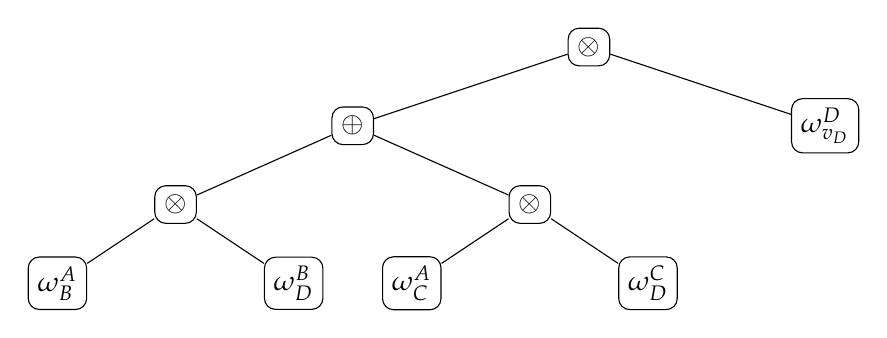
\begin{tikzpicture}[
level distance=1cm,
level 1/.style={sibling distance=6cm},
level 2/.style={sibling distance=4.5cm},
level 3/.style={sibling distance=3cm},
every node/.style={draw, rectangle, rounded corners, align=center},
edge from parent/.style={draw}
]

\node {$\otimes$}
    child {
        node {$\oplus$}
        child {
            node {$\otimes$}
            child { node {$\omega^A_B$} }
            child { node {$\omega^B_D$} }
        }
        child {
            node {$\otimes$}
            child { node {$\omega^A_C$} }
            child { node {$\omega^C_D$} }
        }
    }
    child {
        node {$\omega^D_{v_D}$}
    };

\end{tikzpicture}
\caption{Binary tree representation of the trust expression for the \ac{IMA} usecase}
\label{fig:trust_expression_tree}
\end{figure}

The final phase consists of evaluating the expression using the appropriate fusion and trust discounting operators once the values of the \acp{ATO} have been obtained. In our implementation, the expression is represented as a binary tree in which the leaves correspond to \acp{ATO} and the internal nodes correspond to \ac{SL} operators (\cref{fig:trust_expression_tree}). The evaluation of the expression is therefore performed recursively by propagating opinions from the leaves toward the root of the tree. After recursively evaluating the expression, a final subjective opinion is obtained. This opinion constitutes the \ac{ATL} associated with the original trust proposition $\mathcal{T}(E, P)$.


In summary, the trust assessment process can be performed in three phases:
\begin{enumerate}
    \item Generate an expression by decomposing the trust proposition into simple propositions and using \ac{TNA-SL} on \acp{STN} for each simple proposition.
    \item Quantify the \acp{ATO} in the expression by identifying relevant trust sources, collecting evidence, and applying an appropriate trust opinion quantification model.    
    \item Evaluate the expression using \ac{SL} operators such as fusion and trust discounting in order to derive the \ac{ATL}.
\end{enumerate}

This structured pipeline ensures that trust assessment remains transparent, reproducible, and adaptable across domains. In subsequent chapters, this generic process will be instantiated for dataset trustworthiness, calibration assessment, and \ac{NN} trust propagation.

\todo[inline]{Do I need to add an example? especially since as I said some chapters are already example. TAF paper with Nikos}



\chapter{Optimized \acs{DSPG} Synthesis and Trust Network Analysis with Subjective Logic [By End of March]}
\label{chap:tnasl}
\todo[inline]{Should I mention that this chapters are based on my papers where I contributed with others}
\todo[inline]{Add Evaluation to show the time complexity, especially the Nesting Level Computation}
\section{Introduction}

\acf{TNA-SL}, introduced by J{\o}sang~\cite{10.5555/1151699.1151710}, enables trust reasoning under uncertainty by propagating and aggregating subjective opinions along graph structures. In the methodology introduced in \cref{chap:Trust_method}, \ac{TNA-SL} is used on \ac{STN} to generate the expression in phase I. However, as discussed in \cref{sec:dspg}, a fundamental structural requirement of \ac{TNA-SL} is that the underlying trust network must be a \ac{DSPG}. This structural constraint ensures that trust propagation through discounting and fusion operators is well-defined and yields unambiguous results.

In practice, real-world trust networks rarely satisfy the \ac{DSPG} property. In practical applications trust relationships form complex directed acyclic graphs that contain structural patterns incompatible with DSPG constraints. Consequently, a transformation step, commonly referred to as \ac{DSPG} synthesis, is required prior to trust inference.

\ac{DSPG} synthesis approach proposed in the original work of J{\o}sang~\cite{10.5555/1151699.1151710} incrementally adds branches while verifying structural criteria. 
% As formalized in~\cite{10.1007/978-3-032-08887-1_4}, 
This method relies on overly restrictive conditions and often remove edges considered structurally unsafe. Although this guarantees DSPG compliance, it introduces two major limitations.
\begin{enumerate}
    \item \textbf{Information loss.} Structurally meaningful trust relationships may be discarded, even when they do not fundamentally violate the \ac{DSPG} requirements.
    \item \textbf{Misaligned optimization objective.} Prior approaches implicitly assume that minimizing uncertainty should be the primary objective of synthesis. In practice, preserving as much structural information as possible should be the primary objective.
\end{enumerate}

These observations reveal a structural inefficiency in existing DSPG synthesis methods. The criteria are overly conservative, and the transformation objective is not aligned with information preservation.

At the same time, the \ac{DSPG} analysis phase performed after synthesis suffers from a computational inefficiency. The classical \ac{TNA-SL} reduction (\ac{DSPG} analysis) procedure repeatedly recomputes the \acf{NL} of edges a after each structural transformation. Since \acp{NL} determine the order in which \acp{PPS} are reduced, each reduction step requires a global recomputation of \acp{NL} across the graph. For large trust networks this leads to significant computational overhead and limits the scalability of the analysis procedure.

Finally, classical \ac{SL} trust discounting operators, namely the Two-Edge Path and Multi-Edge Path operators (\cref{table:TD_operators}), assume that the final edge of a path represents functional direct trust. As illustrated in the \ac{IMA} use case, certain network topologies require the discounting of referral-only paths during the reduction process. However, the existing trust discounting operators assume that the final edge of a path represents functional direct trust, which prevents their consistent application in such cases.

Therefore, the limitations of \ac{TNA-SL} are threefold:
\begin{itemize}
    \item A structural limitation caused by overly restrictive \ac{DSPG} synthesis criteria.
    \item An operator-level limitation caused by incomplete trust discounting semantics for referral-only paths.
    \item A computational limitation arising from the repeated recomputation of edge \acp{NL} during \ac{DSPG} analysis, which increases the time complexity of trust inference.
\end{itemize}

This chapter addresses the three aspects in a unified framework.

\subsection*{Unified Optimization Perspective}

We propose an improved \ac{TNA-SL} framework that improves computational efficiency, preserves information, and ensures discounting consistency.

The contributions of this chapter are fourfold.

\begin{enumerate}
    \item \textbf{Refined structural characterization via \ac{PNPS}.} We introduce the concept of \acf{PNPS}, which refines the classical definition of \acf{PPS}. This reformulation provides stronger structural guarantees and enables more efficient detection of DSPG violations.

    \item \textbf{Optimized \ac{DSPG} synthesis criteria.} We derive revised synthesis criteria that admit a strictly larger class of edges while preserving \ac{DSPG} compliance. Unlike prior strategies, the proposed approach prioritizes maximal information retention during synthesis.
    
    \item \textbf{Optimized \ac{DSPG} analysis algorithm.}
    By operating on \ac{PNPS} structures rather than \ac{PPS}, the proposed algorithm ensures structural isolation during reductions and streamlines the computation of \acp{NL}, thereby reducing unnecessary recomputations. We formally establish the corresponding \ac{NL} preservation properties.
    \todo[inline]{add: Optimized algorithm  for DSPG Synthesis, }

    \item \textbf{Referral-edge path discounting operator.} To resolve inconsistencies in referral-only chains, we introduce a novel trust discount operator that extends \ac{SL} discounting semantics to paths composed entirely of referral edges. The proposed operator is compatible with existing Two-Edge and Multi-Edge operators and preserves expected trust attenuation properties across increasing path lengths~\cite{10706345}.
\end{enumerate}
Taken together, these contributions make \ac{TNA-SL} more general, more information-preserving, and more computationally efficient. As a result, the framework becomes better suited for complex systems such as \acp{NN}, where trust must be propagated across heterogeneous and potentially unreliable information sources.

The remainder of this chapter formalizes the proposed framework. Section~\ref{sec:pnps} introduces the \ac{PNPS} concept and the associated structural reformulation.  Section~\ref{sec:optimized_criteria} presents the optimized \ac{DSPG} synthesis criteria. Section~\ref{sec:optimized_analysis} details the optimized analysis algorithm and establishes its correctness properties. Section~\ref{sec:referral_path_operator} introduces the new referral-edge discount operator and analyzes its compatibility with classical Subjective Logic operators. Section~\ref{sec:eval_tnasl} presents the evaluation. Finally, Section~\ref{sec:summary_tnsl} concludes the chapter.

\section{Parallel Non-Intersecting Path Subnetworks}
\label{sec:pnps}

To address the limitations of \ac{DSPG} synthesis and analysis procedures identified in the introduction, we refine the notion of \ac{PPS} originally used in \ac{DSPG} analysis. While \ac{PPS} structures are sufficient for defining the classical \ac{DSPG} reductions order, they are not strong enough to guarantee structural isolation during analysis and \ac{NL} updates. 

For example, consider the graph shown in \cref{fig:ppsv}. If the \ac{PPS} between nodes \(A\) and \(C\) is reduced into a single edge \(AC\), the \ac{NL} of this newly created edge becomes \(0\), while the \acp{NL} of the remaining edges decrease by one. This global update illustrates that reductions based solely on \ac{PPS} structures do not preserve local structural isolation during the reduction process. To overcome this limitation, we introduce a stricter structural construct called the \acf{PNPS}. This refinement plays a central role in enabling both a clearer formalization of \ac{DSPG} structures and stable \ac{NL} computation after \ac{PNPS} reduction into a single edge.

\begin{definition}[\aclu{PNPS}]
\label{def:pnps}
Let $(A,B)$ be a \aclu{PPS} (\cref{def:pps}). It is called a \ac{PNPS} if and only if there exist at least two non-intersecting directed paths from the source $A$ to the sink $B$.
\end{definition}
The key difference between \ac{PPS} and \ac{PNPS} lies in the non-intersection requirement. This distinction is illustrated in \cref{fig:pnps}. For instance, although $(A,G)$ qualifies as a \ac{PPS}, it is not a \ac{PNPS} because we cannot find two non-intersecting paths between $A$ and $G$.

\begin{figure}[]
    \centering
    \begin{subfigure}{0.49\textwidth}
        \centering
        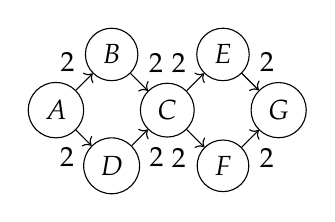
\begin{tikzpicture}[main/.style = {draw, circle}] 
        \node[main] (1) {$A$}; 
        \node[main] (2) [above right of=1] {$B$};
        \node[main] (3) [below right of=1] {$D$}; 
        \node[main] (4) [below right of=2] {$C$};
        \node[main] (5) [above right of=4]{$E$}; 
        \node[main] (6) [below right of=4] {$F$};
        \node[main] (7) [below right of=5] {$G$};
        \draw[->] (1) -- node[midway, above left]{2} (2);
        \draw[->] (1) --  node[midway, below left]{2} (3);
        \draw[->] (2) -- node[midway, above right]{2} (4);
        \draw[->] (3) -- node[midway, below right]{2} (4);
        \draw[->] (4) -- node[midway, above left]{2} (5);
        \draw[->] (4) --  node[midway, below left]{2} (6);
        \draw[->] (5) -- node[midway, above right]{2} (7);
        \draw[->] (6) -- node[midway, below right]{2}  (7);
        \end{tikzpicture}
        \caption{PPS edges NL before reduction}
        \label{fig:ppsv}
    \end{subfigure}
    \hfill
    \begin{subfigure}{0.49\textwidth}
        \centering
        \begin{tikzpicture}[main/.style = {draw, circle}] 
        \node[main] (1) {$A$}; 
        \node[main] (4) [below right of=2] {$C$};
        \node[main] (5) [above right of=4]{$E$}; 
        \node[main] (6) [below right of=4] {$F$};
        \node[main] (7) [below right of=5] {$G$};
        \draw[->, red] (1) -- node[midway, above]{0} (4);
        \draw[->] (4) -- node[midway, above left, text=red]{1} (5);
        \draw[->] (4) --  node[midway, below left, text=red]{1} (6);
        \draw[->] (5) -- node[midway, above right, text=red]{1} (7);
        \draw[->] (6) -- node[midway, below right, text=red]{1}  (7);
        \end{tikzpicture}
        \caption{PPS edges NL after reduction}
        \label{fig:ppsv}
    \end{subfigure}
    \hfill
    \begin{subfigure}{0.49\textwidth}
        \centering
        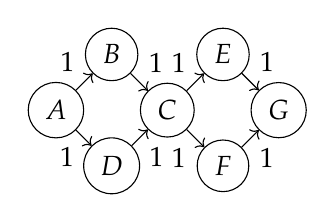
\begin{tikzpicture}[main/.style = {draw, circle}] 
        \node[main] (1) {$A$}; 
        \node[main] (2) [above right of=1] {$B$};
        \node[main] (3) [below right of=1] {$D$}; 
        \node[main] (4) [below right of=2] {$C$};
        \node[main] (5) [above right of=4]{$E$}; 
        \node[main] (6) [below right of=4] {$F$};
        \node[main] (7) [below right of=5] {$G$};
        \draw[->] (1) -- node[midway, above left]{1} (2);
        \draw[->] (1) --  node[midway, below left]{1} (3);
        \draw[->] (2) -- node[midway, above right]{1} (4);
        \draw[->] (3) -- node[midway, below right]{1} (4);
        \draw[->] (4) -- node[midway, above left]{1} (5);
        \draw[->] (4) --  node[midway, below left]{1} (6);
        \draw[->] (5) -- node[midway, above right]{1} (7);
        \draw[->] (6) -- node[midway, below right]{1}  (7);
        \end{tikzpicture}
        \caption{ \ac{PNPS} edges NL before reduction}
        \label{fig:pnpsv}
    \end{subfigure}
    \begin{subfigure}{0.49\textwidth}
        \centering
        \begin{tikzpicture}[main/.style = {draw, circle}] 
        \node[main] (1) {$A$}; 
        \node[main] (4) [below right of=2] {$C$};
        \node[main] (5) [above right of=4]{$E$}; 
        \node[main] (6) [below right of=4] {$F$};
        \node[main] (7) [below right of=5] {$G$};

        \draw[->, red] (1) -- node[midway, above]{0} (4);
        \draw[->] (4) -- node[midway, above left]{1} (5);
        \draw[->] (4) --  node[midway, below left]{1} (6);
        \draw[->] (5) -- node[midway, above right]{1} (7);
        \draw[->] (6) -- node[midway, below right]{1}  (7);
        \end{tikzpicture}
        \caption{ \ac{PNPS} edges NL after reduction}
        \label{fig:pnpsv}
    \end{subfigure}
    \caption{Comparison of \ac{PPS} and  \ac{PNPS}}
    \label{fig:pnps}
\end{figure}


% \subsection{Structural Characterization of Non-DSPG}

The introduction of  \ac{PNPS} enables a simplified structural characterization of non-\ac{DSPG} graphs.

\begin{proposition}[\ac{DSPG} Structural Constraint]
\label{prop:dspg}
A directed acyclic graph is not a \ac{DSPG} if and only if there exists a  \ac{PNPS} whose intermediate node has either:
\begin{itemize}
    \item an outgoing edge to a node outside the  \ac{PNPS} (before reaching its target), or
    \item an incoming edge from a node outside the  \ac{PNPS} (before first reaching its source).
\end{itemize}
\end{proposition}

This proposition provides an operational detection rule. A \ac{PNPS} that satisfies this property cannot be safely reduced to a single edge, as doing so would violate the structural constraints required for a \ac{DSPG}. By focusing exclusively on \ac{PNPS} structures, we obtain stronger structural guarantees and simpler verification conditions.

\section{Optimized \acs{DSPG} Synthesis Criteria}
\label{sec:optimized_criteria}

As discussed in \cref{sec:dspg}, the original \ac{SL} work defines a set of criteria to be used when synthesizing a \ac{DSPG} from a non-\ac{DSPG} graph. Using the \ac{PNPS} definition introduced earlier, we reformulate these criteria in structural terms.

\begin{corollary}[\ac{PNPS}-Based DSPG Criteria]
\label{cor:pnps-criteria}
Let $A$ and $B$ be two nodes of the current graph which is assumed to be a \ac{DSPG}. Adding a branch from $A$ to $B$ preserves the DSPG property if and only if:

\begin{itemize}
    \item \textbf{Criterion 1}: There exists at least one path from $A$ to $B$ in the current graph.
    \item \textbf{Criterion 2}: If $A$ is an intermediate node of a \ac{PNPS} $P$, then $B$ must also be an intermediate node of $P$, and conversely.
\end{itemize}
\end{corollary}

This formulation replaces \ac{NNL} arithmetic conditions with a structural containment rule. It directly captures part of the isolation constraint established in \cref{prop:dspg}.

Before establishing the equivalence between the original \ac{NNL}-based criteria and the structural \ac{PNPS}-based formulation, we introduce an alternative characterization of the \ac{NNL}. While the classical definition of \ac{NNL} is expressed as a counting measure over \acp{PPS}, the structural interpretation of \ac{DSPG} graphs suggests a formulation in terms of the nesting depth of \acp{PNPS}. The following theorem shows that the nesting level of a node can equivalently be expressed as the maximum nesting level of the \acp{PNPS} in which the node appears as an intermediate node. This result provides the bridge between the arithmetic \ac{NNL} formulation and the structural containment rules used in the \ac{PNPS}-based criteria.

\begin{theorem}[\ac{PNPS}-Based Characterization of \ac{NNL}]
\label{thm:pnps-nnl}
Let $G$ be a \ac{DSPG} and let $v$ be a node of $G$. Then
\begin{align}
\label{eq:pnps-nnl}
\mathrm{NNL}_G(v) = 
\max\left\{
\mathrm{PNL}_G(P)
\;\middle|\;
P\in\mathcal{P}_G,\;
v \text{ is an intermediate node of } P
\right\}, 
\end{align}

where
\[
\mathrm{PNL}_G(P)
=
\min\left\{
\mathrm{NL}_G(e)
\;\middle|\;
e \text{ is an edge of } P
\right\},
\]
with the convention that the maximum over the empty set is $0$.
\end{theorem}
Intuitively, in a \ac{DSPG} the \ac{PNPS} containing a node are nested. The nesting level of the node therefore corresponds to the deepest \ac{PNPS} surrounding it.

\begin{proof}
By definition,
\[
\mathrm{NNL}_G(v)=
\left|
\left\{
P\in\mathcal{P}_G
\;\middle|\;
v \text{ is an intermediate node of } P
\right\}
\right|.
\]

Thus, $\mathrm{NNL}_G(v)$ counts the number of \acp{PNPS} in which $v$
appears as an intermediate node.

Let
\[
\mathcal{P}_G(v)=
\left\{
P\in\mathcal{P}_G
\;\middle|\;
v \text{ is an intermediate node of } P
\right\}
\]
denote the set of \acp{PNPS} in which $v$ appears as an intermediate node.

If $\mathcal{P}_G(v)=\emptyset$, then by definition $\mathrm{NNL}_G(v)=0$.
The right-hand side of \cref{eq:pnps-nnl} is also the maximum over the empty set,
which by convention equals $0$. Hence the equality holds.

Assume now that $\mathcal{P}_G(v)\neq\emptyset$.
Because $G$ is a \ac{DSPG}, the \acp{PNPS} containing $v$ as an intermediate node
must be nested. Indeed, if two such subnetworks $P_1$ and $P_2$ were not nested,
it would be possible to exit $P_1$ toward $P_2$ (or vice versa) without first
reaching the target of $P_1$, which contradicts the \ac{DSPG} structural constraint
(\cref{prop:dspg}). Therefore the elements of $\mathcal{P}_G(v)$ form a chain
under inclusion.

Let
\[
P^\star \in \mathcal{P}_G(v)
\]
be the most nested \ac{PNPS} in this chain. Since $P^\star$ is contained in
all other subnetworks of $\mathcal{P}_G(v)$, every edge of $P^\star$ belongs
to every $P \in \mathcal{P}_G(v)$. Hence, for any edge $e \in P^\star$,
\[
e \in P^\star \Rightarrow e \in P, \quad \forall P\in\mathcal{P}_G(v).
\]

Therefore each such edge belongs to at least $|\mathcal{P}_G(v)|$ subnetworks,
which implies
\[
\mathrm{NL}_G(e)\ge |\mathcal{P}_G(v)|.
\]

By definition of $\mathrm{PNL}$,
\[
\mathrm{PNL}_G(P^\star)
=
\min\left\{
\mathrm{NL}_G(e)
\;\middle|\;
e \text{ is an edge of } P^\star
\right\},
\]
and thus
\begin{equation}
    \label{eq:proof_nnl_1}
    \mathrm{PNL}_G(P^\star)\ge |\mathcal{P}_G(v)|.
\end{equation}

Conversely, consider an edge $e_v\in P^\star$ whose sink is $v$.
Let $P\in\mathcal{P}_G$ be a \ac{PNPS} such that $e_v\in P$.
Since $P^\star$ is the most nested \ac{PNPS} containing $v$, it follows from the
\ac{DSPG} structural constraint (\cref{prop:dspg}) that
\[
e_v\in P \;\Rightarrow\; P^\star\subseteq P .
\]

Indeed, $v$ cannot be the target of $P$. Otherwise, it would be possible to exit $P$ and enter $P^\star$ through $v$ without first reaching the source of $P^\star$, which contradicts the \ac{DSPG} structural constraint.

Hence $v$ must be an intermediate node of $P$, which implies $P\in\mathcal{P}_G(v)$.

Therefore
\[
\left|
\left\{
P\in\mathcal{P}_G
\;\middle|\;
e_v\in P
\right\}
\right|
\le
|\mathcal{P}_G(v)|.
\]

Since $\mathrm{NL}_G(e_v)$ counts exactly this quantity, we obtain
\[
\mathrm{NL}_G(e_v)\le |\mathcal{P}_G(v)|.
\]

Because $\mathrm{PNL}_G(P^\star)$ is the minimum $\mathrm{NL}$ among the edges
of $P^\star$, it follows that
\begin{equation}
\label{eq:proof_nnl_2}
    \mathrm{PNL}_G(P^\star)\le |\mathcal{P}_G(v)|.
\end{equation}



Combining the two inequalities yields \cref{eq:proof_nnl_1,eq:proof_nnl_2}
\[
\mathrm{PNL}_G(P^\star)=|\mathcal{P}_G(v)|.
\]
Finally, 
\begin{align}
\mathrm{NNL}_G(v) &= |\mathcal{P}_G(v)| \notag \\
&= \mathrm{PNL}_G(P^\star) \notag \\
&= \max\left\{
\mathrm{PNL}_G(P)
\;\middle|\;
P\in\mathcal{P}_G,\; 
v \text{ is an intermediate node of } P
\right\}. \notag
\end{align}

This proves the claim.
\end{proof}

\begin{theorem}[Equivalence of Criteria]
\label{thm:criteria-equivalence}
When the current graph is \ac{DSPG} (\cref{def:dspg_original_criteria}), J{\o}sang's original criteria are logically equivalent to the \ac{PNPS}-based DSPG criteria of \cref{cor:pnps-criteria}.
\end{theorem}

\begin{lemma}\label{lemma}
Let $H$, $I$, $J$, and $K$ be logical statements. Suppose we want to prove the equivalence:
\[
(H \wedge I) \Leftrightarrow (J \Leftrightarrow K).
\]
We can analyze this equivalence using contrapositive reasoning as follows.

First, recall that:
\[
\neg(H \wedge I) = \neg H \vee \neg I
\]
and
\[
\neg(J \Leftrightarrow K) = \neg\left((J \Rightarrow K) \wedge (K \Rightarrow J)\right) = (J \wedge \neg K) \vee (K \wedge \neg J).
\]

Therefore, proving the equivalence:
\(
(H \wedge I) \Leftrightarrow (J \Leftrightarrow K)
\)
is logically equivalent to proving:
\[
(J \wedge \neg K) \vee (K \wedge \neg J) \Leftrightarrow \neg H \vee \neg I.
\]

In particular, if we only want to prove a one-way implication:
\(
(H \wedge I) \Rightarrow (J \Rightarrow K),
\)
we can equivalently prove the contrapositive:
\[
(J \wedge \neg K) \Rightarrow (\neg H \vee \neg I).
\]
\end{lemma}

\noindent We apply this lemma in the proofs of \cref{thm:criteria-equivalence,thm:optimized-sound}.

\begin{proof}
The proof is based on the logical structure outlined in Lemma~\ref{lemma}

We want to prove that $NNL(A) = NNL(B)$, and that all intermediate node $C$ between $A$ and $B$ should have $NNL(C) \geq NNL(A) \Leftrightarrow A$ is an intermediate node of a PNPS $P$ if and only if $B$ is an intermediate node of $P$.

($\Rightarrow$)
If $A$ is an intermediate node of a PNPS $P$ and $B$ is not. This means that the sink $C$ of $P$ is before $B$ in a path from $A$ to $B$. Therefore, $NNL(C)<NNL(A)$. The same logic applies when $B$ is an intermediate node of a PNPS $P$ and $A$ is not.
    
($\Leftarrow$) If $NNL(A) \neq NNL(B)$ then by definition we can find a PNPS in which one node ($A$ or $B$) is an intermediate node, but the other not.
\end{proof}


% \subsection{Optimized Criteria}

Although equivalent to the original formulation, the \ac{PNPS}-based perspective reveals that strict equality of \acp{NNL} is not strictly necessary. Structural correctness is preserved as long as no  \ac{PNPS} isolation constraint is violated. We therefore introduce optimized criteria.

\begin{definition}[Optimized DSPG Synthesis Criteria]
\label{def:optimized-criteria}
A branch from $A \to B$ can be safely added if and only if:

\begin{itemize}
    \item \textbf{Criterion 1:} There exists a path from $A$ to $B$.
    \item \textbf{Criterion 2:} 
    \begin{enumerate}
        \item If $A$ is an intermediate node of a  \ac{PNPS} $P$, then $B$ must lie inside $P$.
    \item If $B$ is an intermediate node of a  \ac{PNPS} $P$, then $A$ must lie inside $P$.
\end{enumerate}
\end{itemize}
\end{definition}

The difference compared to the original criteria is that we allow $A$ or $B$ to be the source or target of the same \ac{PNPS}, not necessarily intermediate nodes. This strictly enlarges the admissible class of branches.

% \subsection{Soundness and Completeness}

\begin{figure}
    \centering
    \begin{subfigure}{0.49\textwidth}
    \centering
    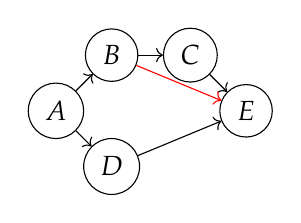
\begin{tikzpicture}[main/.style = {draw, circle}] 
        \node[main] (1) {$A$}; 
        \node[main] (2) [above right of=1] {$B$};
        \node[main] (3) [below right of=1] {$D$}; 
        \node[main] (4) [right of=2] {$C$};
        \node[main] (5) [below right of=4] {$E$}; 
        \draw[->] (1) -- (2);
        \draw[->] (1) -- (3);
        \draw[->] (2) -- (4);
        \draw[->] (4) -- (5);
        \draw[->] (3) -- (5);
        \draw[red, ->] (2) -- (5);
        % \draw[red, ->] (1) -- (4);
    \end{tikzpicture} 
    \caption{Sub-optimality of Original Criteria}
    \label{fig:ex}
    \end{subfigure}
    \begin{subfigure}{0.49\textwidth}
\centering
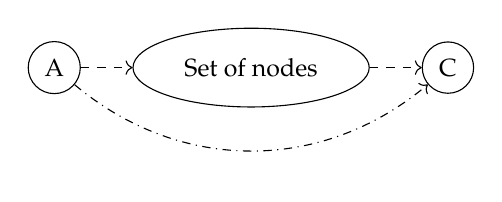
\begin{tikzpicture}[node distance=2.5cm, every node/.style={font=\small}]
    % Nodes
    \node[circle, draw] (A) {A};
    \node[ellipse, draw, minimum width=3cm, minimum height=1cm, right of=A] (middle) {Set of nodes};
    \node[circle, draw, right of=middle] (C) {C};

    % Dashed path through middle
    \draw[dashed, ->] (A) -- (middle);
    \draw[dashed, ->] (middle) -- (C);

    % Dotted shortcut from A to B
    \draw[dash dot, ->] (A) to[bend right=40] (C);
\end{tikzpicture}
\caption{New maximal-NL PNPS after edge addition}
\label{fig:pr}
\end{subfigure}
\caption{Illustrative example supporting the proof of the DSPG synthesis criteria}
\end{figure}


\begin{theorem}[Soundness and Completeness]
\label{thm:optimized-sound}
Let $A \rightarrow B$ be a candidate branch.

\begin{enumerate}
    \item If the branch satisfies the optimized criteria, the resulting graph remains \ac{DSPG}. \label{thm:firstpart}
    \item If adding the branch does not violate the \ac{DSPG} property, then the branch satisfies the optimized criteria. \label{thm:secondpart}
\end{enumerate}
\end{theorem}

\begin{proof}
This proof is based on the logical structure outlined in Lemma~\ref{lemma}

For \ref{thm:firstpart}: We know that if $A$ is an intermediate node of a PNPS $p$ then $B$ is an intermediate node of $p$ and if $B$ is an intermediate node of a PNPS $p$ then $A$ is an intermediate node of $p$ implies that the DSPG property not broken. What we need to show in this proof is that adding an edge from the source to an intermediate node or from an intermediate node to the sink inside a PNPS $p$ with maximum Nesting Level does not affect the DSPG property of the graph. We are doing the proof for the maximum NL because it is the same as doing the proof for any PNPS since what we want to know is whether we can still reduce a PNPS to a single edge using the DSPG analysis algorithm depicted in Figure~\ref{fig:algsynth2}. During the reduction process, the reduction will be done for this PNPS when the PNPS will be the most nested (the PNPS with maximum Nesting Level).
    \begin{itemize}
        \item add an edge from the source $A$ to an intermediate node $C$:
        Assuming that the current PNPS has max NL, adding this branch does not break the DSPG property because after adding this branch the max NL will be increased by one. Then the new PNPS with maximum NL will be the new one created  $[A,C]$. This new PNPS will be like Figure~\ref{fig:pr} because it is clear that there is only one path from $A$ to $C$ otherwise $A$ and $C$ would have been the source and sink of a PNPS with NL greater than NL of $p$.
    
        \item add an edge from an intermediate node $C$ to the target $B$: Same logic as before. We can just reverse the graph and use the same proof.
    \end{itemize}

    
For \ref{thm:secondpart}: $A$ to $B$ does not break DPSG property. Assuming that the first criterion of criteria defined in \cref{cor:pnps-criteria} is fulfilled, then \cref{prop:dspg} implies that $A$ to $B$ fulfilled Criterion 2 of the optimized Criteria for DSPG Synthesis.
\end{proof}
% \paragraph{Nesting-Level Formulation}

The optimized criteria admit a simple arithmetic restatement in terms of \ac{NNL}.

\begin{theorem}[\ac{NNL} Reformulation of the Optimized Criteria]
\label{thm:nnl-reformulation}
The optimized criteria are equivalent to:

\begin{itemize}
    \item \textbf{Criterion 1}: A path from $A$ to $B$ exists.
    \item \textbf{Criterion 2}:
    \begin{enumerate}
        \item $|\mathrm{NNL}(A) - \mathrm{NNL}(B)| \leq 1$.
        \item Every intermediate node $C$ between $A$ and $B$ satisfies
        \[
        \mathrm{NNL}(C) \geq \min(\mathrm{NNL}(A), \mathrm{NNL}(B)).
        \] 
    \end{enumerate}
\end{itemize}
\end{theorem}

The only difference from the original criteria is that equality of \acp{NNL} is relaxed to a difference of at most one. This relaxation precisely captures admissible additions from a \ac{PNPS} source to its intermediate nodes or from intermediate nodes to its target.


In summary, the optimized criteria provide three improvements:

\begin{enumerate}
    \item They strictly generalize the original criteria.
    \item They preserve \ac{DSPG} correctness.
    \item They maximize information retention.
\end{enumerate}

These criteria form the logical foundation for the optimized synthesis algorithm presented in the next section.


\section{Optimized \acs{DSPG} Synthesis Algorithm}
\label{sec:optimized_algorithm}

In previous \cref{sec:optimized_criteria}, we established necessary and sufficient conditions under which a branch can be added to a \ac{DSPG} without violating structural constraints. We now present a constructive algorithm that implements these criteria and synthesizes a \ac{DSPG} from an arbitrary directed acyclic graph. The algorithm incrementally builds a \ac{DSPG} by selecting admissible branches according to the optimized criteria while maintaining structural information about  \ac{PNPS} membership.

% \subsection{Algorithm Overview}

Let $G = (V,E)$ be a directed acyclic graph that may not satisfy the DSPG property. The synthesis procedure constructs a subgraph $G' \subseteq G$ that is DSPG-compliant. The key idea is based on previous work~\cite{4622580}:
\begin{enumerate}
    \item Enumerate all source-to-sink paths in $G$.
    \item Initialize $G'$ with one valid path.
    \item Iteratively attempt to add remaining branches.
    \item Accept a branch if and only if it satisfies the optimized criteria.
\end{enumerate}

To efficiently evaluate structural conditions, we maintain a mapping
\[
nodeToPNPS : V \rightarrow \{\text{highest nested  \ac{PNPS} containing the node}\}.
\]

This mapping allows constant-time verification of \ac{PNPS} containment constraints.

% \subsection{Algorithm Description}

Algorithm~\ref{alg:dspg-synth} presents the synthesis procedure.
\begin{algorithm}[H]
\caption{Optimized DSPG Synthesis}
\label{alg:dspg-synth}
\begin{algorithmic}[1]
\Require Directed acyclic graph $G = (V,E)$
\Ensure DSPG subgraph $G' \subseteq G$
\State $paths \gets$ GetAllPaths($G$)
\State Sort $paths$ by uncertainty or length
\State $G' \gets$ $paths.pop()$ \Comment{Initialize with first path}
\State $nodeToPNPS \gets \emptyset$
\While{$paths \neq \emptyset$}
    \State $path \gets paths.pop()$
    \State $branch \gets$ first branch of $path$ not in $G'$
    \State $(A,B) \gets (source(branch), target(branch))$
    \State $check \gets$ DSPGChecker($nodeToPNPS$, $A$, $B$)
    \If{$check.bool = \text{True}$}
        \State $G'.addEdges(branch)$

        \State UpdatePNPS($nodeToPNPS$, $check.intermediateNodes$,$branch.intermediateNodes$, $(A,B)$)

    \EndIf
\EndWhile
\end{algorithmic}
\end{algorithm}

\begin{algorithm}
\caption{UpdatePNPS}
\label{alg:update-pnps}
\begin{algorithmic}[1]
\Require $nodesToPNPS$ : current map from node $\rightarrow$ PNPS
\Require branch $BranchListOfIntermediateNodes$
\Require checker $CheckerListOfIntermediateNodes$
\Require $(nodeSource, nodeTarget)$ : candidate PNPS

\Ensure $nodesToPNPS$ maps each node to the **highest nested PNPS** it is part of

\For{$v \in$ $CheckerListOfIntermediateNodes$}
\State $nodesToPNPS[v] \gets smallerPNPS((nodeSource, nodeTarget),\ nodesToPNPS[v])$
\EndFor

\For{v $\in$ $BranchListOfIntermediateNodes$}
\State $nodesToPNPS[v] \gets moreNestedPNPS((nodeSource, nodeTarget),\ nodesToPNPS[v])$
\EndFor

\State \Return $nodesToPNPS$

\end{algorithmic}
\end{algorithm}


The function \texttt{DSPGChecker} verifies the optimized criteria:
\begin{enumerate}
    \item Existence of a path from $A$ to $B$.
    \item Structural containment consistency according to Definition~\ref{def:optimized-criteria}.
\end{enumerate}
\todo[inline]{Add text regarding DSPGChecker algorithm}
\begin{algorithm}
\caption{DSPG Local Checker}
\begin{algorithmic}[1]
\Require Dictionary $\textit{nodesToPNPS}$, source node $src$, target node $target$
\If{there is a path from $src$ to $target$}
    \State $pathNodes \gets$ list of all intermediate nodes in this path
\Else
    \State \Return $\{bool: False\}$
\EndIf

\If{$nodesToPNPS[src] \neq None$}
    \If{$target \notin nodesToPNPS[src]$}
        \State \Return $\{bool: False\}$
    \EndIf
\EndIf

\If{$nodesToPNPS[target] \neq None$}
    \If{$src \notin nodesToPNPS[target]$}
        \State \Return $\{bool: False\}$
    \EndIf
\EndIf

\State \Return $\{bool: True,\; intermediateNodes: pathNodes\}$
\end{algorithmic}
\end{algorithm}

Following we show different properties of the \cref{alg:dspg-synth}.

The correctness of the algorithm relies on the invariant that $nodesToPNPS[v]$ always stores the most deeply nested  \ac{PNPS} in which node $v$ appears as an intermediate node.
\begin{theorem}
Let $a$ and $b$ be two nodes, and assume that we have a mapping 
$nodesToPNPS$ which maps a node to the highest nested PNPS it is part of.
Then we have

\begin{align}
    nodesToPNPS[a] = None \;\text{ or }\; b \in nodesToPNPS[a]
\iff \notag \\
\text{if node } a \text{ is an intermediate node of a PNPS } p
\text{ then } b \text{ is inside } p . \notag 
\end{align}


\end{theorem}
\begin{proof}

($\Rightarrow$)
If $nodesToPNPS[a] = None$, then $a$ is not part of any PNPS.
Therefore the second statement is trivially true.

If $b \in nodesToPNPS[a]$, then $b$ belongs to the most nested PNPS
containing $a$. Since every PNPS containing $a$ also contains
$nodesToPNPS[a]$, it follows that $b$ is part of any PNPS that
contains $a$.

($\Leftarrow$)
If node $a$ is an intermediate node of a PNPS $P$ and $b$ is inside $P$,
then $b$ belongs to every PNPS of which $a$ is an intermediate node.
Since $nodesToPNPS[a]$ represents the most nested PNPS containing $a$,
it follows that $b \in nodesToPNPS[a]$.

\end{proof}

\begin{theorem}
The update of $nodesToPNPS$ in \cref{alg:update-pnps} ensures that $nodesToPNPS$ maps each node to the highest nested PNPS it is part of.
\end{theorem}
\begin{proof}

We want to prove that if before the update of $nodesToPNPS$ the mapping
associates each node with the highest nested PNPS it belongs to,
then after the update this property still holds.

When adding a new branch from $A \to B$, two situations may occur.

\textbf{Case 1:} The subnetwork from $A$ to $B$ was already a PNPS.
In this case, the update only assigns values to the newly added nodes,
while the existing nodes already have the correct mapping.

\textbf{Case 2:} The subnetwork from $A$ to $B$ forms a new PNPS.
Two subcases arise.

\begin{itemize}

\item \textbf{No PNPS between $A$ and $B$.}  
A new PNPS is created. The intermediate nodes of this PNPS are exactly
the nodes on the branch being added and the intermediate nodes on the
path from $A$ to $B$ before adding the branch. These nodes are therefore
updated to map to this newly created PNPS.

\item \textbf{Existing PNPS between $A$ and $B$.}  
Some intermediate nodes on the path from $A$ to $B$ may already belong
to a more nested PNPS. For these nodes, $nodesToPNPS$ is not updated
because they already map to a more nested PNPS. The nodes that are not
part of a more nested PNPS are updated accordingly. This is valid
because every path from $A$ to $B$ before adding the new branch
contains these nodes, meaning they are not intermediate nodes of any
PNPS between $A$ and $B$.

\end{itemize}

Therefore, after the update, each node still maps to the highest nested
PNPS it belongs to.

\end{proof}

\begin{theorem}[Algorithm Soundness]
\label{thm:alg-sound}
At every iteration, $G'$ remains DSPG.
\end{theorem}

\begin{proof}
The algorithm adds a branch only if it satisfies the optimized synthesis criteria of \cref{thm:optimized-sound}. By soundness of those criteria, the addition preserves the DSPG property. Since the initial path is trivially DSPG and each step preserves the invariant, the resulting graph remains DSPG.
\end{proof}

\begin{theorem}[Algorithm Completeness]
\label{thm:alg-complete}
If a branch can be added without violating the DSPG property, the algorithm will accept it.
\end{theorem}

\begin{proof}
By completeness of the optimized criteria in \cref{thm:optimized-sound}, any branch that preserves DSPG must satisfy the structural containment conditions. The \texttt{DSPGChecker} verifies exactly these conditions. Therefore admissible branches are not rejected.
\end{proof}

% \subsection{Termination}

\begin{theorem}[Termination]
\label{thm:termination}
The algorithm terminates after a finite number of iterations.
\end{theorem}

\begin{proof}
The number of paths in a finite directed acyclic graph is finite. At each iteration, one path is removed from the list and processed. No path is reinserted. Therefore the algorithm terminates.
\end{proof}

% \subsection{Complexity Considerations}

Let $P$ denote the number of source-to-sink paths in $G$.

\begin{itemize}
    \item Path enumeration is exponential in the worst case.
    \item Each branch verification is constant time assuming $nodeToPNPS$ is maintained efficiently.
    \item  \ac{PNPS} updates are linear in the size of the branch.
\end{itemize}

Although path enumeration may be expensive in theory, in trust networks the graph structure is typically sparse and limited in depth. Moreover, synthesis is performed once prior to trust inference, making preprocessing cost acceptable.

% \subsection{Structural Implications}

This completes the structural synthesis component of the framework. In the next section, we turn to optimized DSPG analysis and \acp{NL} computation during reduction.

\section{Optimized \acs{DSPG} Analysis and \acs{PNPS}-Based Reduction}
\label{sec:optimized_analysis}

Once a \ac{DSPG} graph has been synthesized, trust inference proceeds through structural reduction. Classical \ac{DSPG} analysis reduces the graph recursively by collapsing \ac{PPS} into single edges until only one edge remains between the global source and sink.

In this section, we demonstrate that replacing \ac{PPS} with  \ac{PNPS} leads to a more stable and structurally isolated reduction process. We formalize the reduction procedure and analyze nesting-level evolution.

% \subsection{PNPS-Based Reduction Principle}

In the classical formulation, a \ac{DSPG} is recursively reduced using two operations:
\begin{enumerate}
    \item Series reduction, which collapses two consecutive edges incident to a node of degree two.
    \item Parallel reduction, which collapses parallel edges into a single edge.
\end{enumerate}

\todo[inline]{the following is not clear at all} In the \ac{PPS}-based framework, identifying valid parallel structures may require global structural reasoning. Furthermore, nesting-level updates are implicitly derived and can be difficult to track precisely.





Using \ac{PNPS}, reduction becomes structurally localized.
\begin{definition}[ \ac{PNPS} Reduction]
Let $P$ be a  \ac{PNPS} with source $A$ and target $B$. A  \ac{PNPS} reduction replaces the entire subnetwork $P$ with a single edge $(A,B)$ whose subjective opinion equals the fusion of the discounted opinions along the paths in \(P\).
\end{definition}

The key advantage of \ac{PNPS} is that structural isolation is guaranteed by Definition~\ref{def:pnps} (\cref{fig:pnps}). Since the parallel paths are node-disjoint, collapsing the subnetwork does not create unintended structural interactions.

Reduction proceeds by iteratively selecting a \ac{PNPS} with maximum \ac{NL}.


The optimized analysis algorithm relies on the fact that reducing a  \ac{PNPS} preserves structural consistency and updates \acp{NL} in a controlled manner.

\begin{theorem}[\ac{PNPS}  Reduction Preservation and Nesting Update]
\label{thm:pnps-reduction}
Let $G$ be a \ac{DSPG}, and let $\text{pnps}_1$ be a \ac{PNPS} in $G$ with the maximum Nesting Level. Then:
\begin{enumerate}
    \item \textbf{(Isolated Transformation)} Transforming $\text{pnps}_1$ into a single edge does not affect the Nesting Level of any other PNPS in the graph.
    \item \textbf{(Nesting Level Update)} The edge that replaces $\text{pnps}_1$ has a Nesting Level equal to $\text{NL}(\text{pnps}_1) - 1$.
\end{enumerate}
\end{theorem}
The theorem formalizes two essential properties.

First, reduction is isolated. The transformation of a maximally nested  \ac{PNPS} does not alter the structural hierarchy of remaining  \acp{PNPS}.

Second, \acp{NL} decrease in a strictly controlled manner. This guarantees termination of the reduction process and preserves ordering among nested structures.


The proof of \cref{thm:pnps-reduction} relies on structural relationships between nested  \acp{PNPS}.

Before proving Theorem~\ref{thm:pnps-reduction}, we need to introduce several elementary results that characterize the structural relationships between nested PNPSs. These results are necessary to justify both the isolation property and the nesting level update described above.
\begin{theorem}
\label{thrm:anlsys1}
\label{thrm:anlsys2}
Consider a DSPG and two PNPSs, $pnps_1$ and $pnps_2$, such that $NL(pnps_1) > NL(pnps_2)$. Then:
\begin{enumerate}
    \item \label{thm:p1} If a node $s$ is the common source of both $pnps_1$ and $pnps_2$, then $s$ must have at least one outgoing edge that is in $pnps_2$ but not in $pnps_1$.
    \item \label{thm:p2} If a node $t$ is the common target of both $pnps_1$ and $pnps_2$, then $t$ must have at least one incoming edge that is in $pnps_2$ but not in $pnps_1$.
\end{enumerate}
\end{theorem}

\begin{proof}
\label{prf:anlsys1}
For part~\ref{thm:p1} of the theorem.
If $NL(pnps_1) > NL(pnps_2)$, then $pnps_1$ and $pnps_2$ don't have the same target (since they already have the same source). Thus:
\begin{itemize}
    \item  either $pnps_1$ is inside $pnps_2$: If $s$ does not have at least one outgoing edge to a node which is inside $pnps_2$ and outside $pnps_1$ it means that all paths from $s$ to target of $pnps_2$ will be through $pnps_1$ since from an intermediate node of $pnps_1$ we cannot go outside $pnps_1$ without reaching the target of $pnps_1$. The consequence is that we will not be able to find two non-intersecting paths therefore the graph is not DSPG;
    
    \item or $pnps_1$ is not inside $pnps_2$ and $Nodes(pnps_1) \cap Nodes(pnps_1) \neq \{s\}$: In this case the graph cannot be a DSPG because it means that $pnps_1$ has an intermediate node $n_1$ inside $pnps_2$ (which are not $s$) and a node $n_2$  outside $pnps_2$. $n_2$ is an intermediate node of $pnps_2$ (otherwise it’s the target node of $pnps_2$, and in this case it impossible to have $NL(pnps_1)>NL(pnps_2 )$). Therefore, from $n_1$ (intermediate node of $pnps_2$) we can reach $n_2$ (outside $pnps_2$)  without visiting the target of $pnps_2$
    
    \item or $pnps_1$ is not inside $pnps_2$ and $Nodes(pnps_1) \cap Nodes(pnps_1) = \{s\}$: In this case $s$ has at least one outgoing edge to a node which is inside $pnps_2$ and outside $pnps_1$ 
    
\end{itemize}

The part~\ref{thm:p2} of the theorem is the dual case of item. Reverse the graph and apply the same reasoning.
\end{proof}

\begin{figure}
    \centering
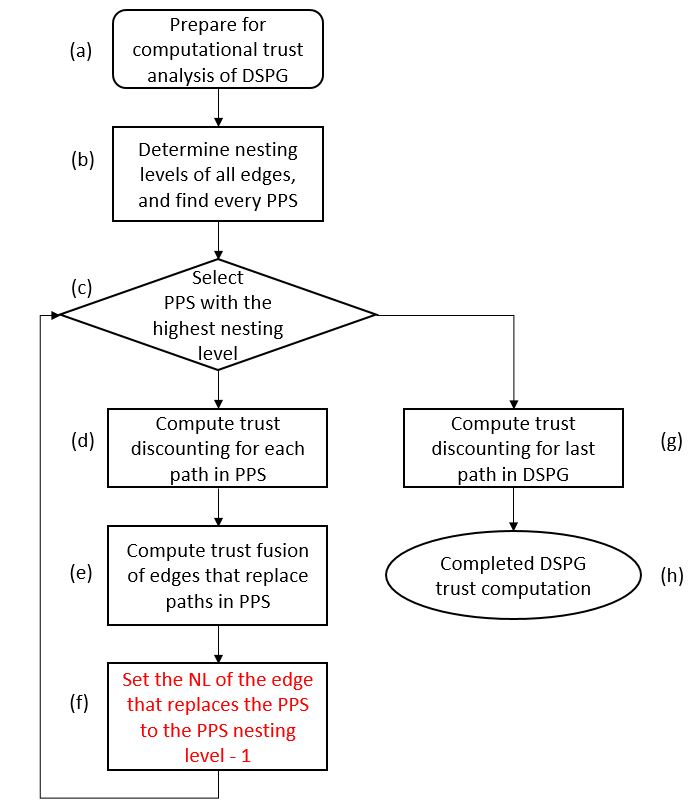
\includegraphics[width=0.5\textwidth]{img/dspg/newsynth.pdf}
    \caption{Our optimized DSPG analysis algorithm}
    \label{fig:algsynth2}
\end{figure}
\begin{corollary}
\label{corol:synth}
Considering a DSPG, if a PNPS $pnps_1$ is nested in another PNPS $pnps_2$ and $pnps_1 \neq pnps_2$, then $pnps_2$ has at least one edge not in $pnps_1$.
\end{corollary}
\begin{proof}
    If a PNPS $pnps_1$ is nested in another PNPS $pnps_2$, we can distinguish between two cases:
\begin{enumerate}
    \item $pnps_1$ and $pnps_2$ do not share the same source and also do not share the same target nodes: if they don't have the same source then the path from the source of $pnps_2$ to the source of $pnps_1$ contains edges outside $pnps_1$. Same reasoning  if they don't have the same target.
    \item $pnps_1$ shares the source or the target (or both) with $pnps_2$: application of Theorems \cref{thrm:anlsys1}.
\end{enumerate}
\end{proof}


We now return to the proof of \cref{thm:pnps-reduction} stated above. 
\begin{proof}
    When reducing a PNPS with the maximum Nesting Level (denoted as $pnps_1$), two structural cases arise:
\begin{enumerate}
    \item $pnps_1$ is a non nested PNPS, or
    \item $pnps_1$  is nested within another PNPS (denoted as $pnps_2$).
\end{enumerate}
In case (1), $pnps_1$ has a Nesting Level equal to 1. After its reduction, all other PNPSs remains the same and the resulting edge has a Nesting Level of 0. In the case (2), since at least one edge --- denoted as $e$ --- in $pnps_2$ is not part of $pnps_1$ (Corrolary~\ref{corol:synth}), $NL(e)$ will remain unchanged and we select it such that its Nesting Level equals that of $pnps_2$ (this follows from  \cref{thrm:anlsys1} with $pnps_1$ Nesting Level equals $pnps_2$ Nesting Level plus 1. Such a PNPS($pnps_2$) exists, as the Nesting Level increments one by one). As a result, the Nesting Level of $pnps_1$ is preserved, since the new edge has Nesting Level reduced by one which is still greater than or equal to that of $pnps_2$.
\end{proof}

\begin{theorem}[Reduction Ordering]
\label{thm:reduction-ordering}
Let $G$ be a DSPG. Reducing a  \ac{PNPS} with maximum \ac{NL} preserves the nesting structure of all remaining  \acp{PNPS}.
\end{theorem}

\begin{proof}
This follows directly from \cref{thm:pnps-reduction}. A maximally nested  \ac{PNPS} is structurally contained within no other \ac{PNPS} of higher \ac{NL}. Therefore its reduction does not modify the structural boundaries of less nested  \acp{PNPS}.
\end{proof}

This ordering guarantees that reduction progresses from the most deeply nested structures outward, ensuring structural consistency.








\subsection{Correctness and Implications for Trust Inference}

Replacing PPS with\ac{PNPS} produces three fundamental improvements:

\begin{enumerate}
    \item \textbf{Stronger isolation guarantees.}  \ac{PNPS} ensures that intermediate nodes cannot connect to external structures without violating DSPG.
    
    \item \textbf{Simplified detection of non-DSPG patterns.} Structural violations become local and verifiable through \cref{prop:dspg}.
    
    \item \textbf{Stable nesting updates.} \cref{thm:pnps-reduction} guarantees predictable nesting-level evolution during reduction.
\end{enumerate}

These properties form the structural backbone of the optimized synthesis and analysis framework presented in the next sections.


\begin{theorem}[Correctness of \ac{PNPS}-Based Reduction]
\label{thm:analysis-correct}
Let $G$ be a DSPG. Iterative \ac{PNPS}-based reduction yields a single edge between the global source and sink whose opinion equals the trust inference result defined by Subjective Logic operators.
\end{theorem}

\begin{proof}
Since every DSPG can be reduced by successive series and parallel reductions, and since  \ac{PNPS} is a stricter form of PPS that preserves structural equivalence, every PPS reduction step is captured by a \ac{PNPS} reduction.

At each reduction step, subjective opinions are combined using valid fusion and discount operators. Because  \ac{PNPS} structures are node-disjoint, operator application is well-defined and free of ambiguity.

Since \acp{NL} decrease strictly and the graph is finite, the process terminates with a single edge representing the global trust evaluation.
\end{proof}


The \ac{PNPS}-based approach improves classical analysis in three aspects:

\begin{enumerate}
    \item \textbf{Structural isolation.} Node-disjointness guarantees reduction does not affect unrelated structures.
    \item \textbf{Deterministic nesting updates.} \acp{NL} decrease in a controlled and predictable manner.
    \item \textbf{Simplified detection.} Structural violations can be identified locally using \cref{prop:dspg}.
\end{enumerate}

In contrast, PPS-based reduction may require global reasoning to ensure that intermediate nodes do not create unintended structural exits.



The \ac{PNPS}-based reduction framework guarantees that:

\begin{itemize}
    \item Every reduction step corresponds to a valid trust operator application.
    \item No structural ambiguity arises during fusion.
    \item Information retention achieved during synthesis is preserved during analysis.
\end{itemize}

This completes the structural component of the optimized framework. We now turn to the operator-level limitation identified previously.








\section{Trust Discounting for Referral Paths}
\label{sec:referral_path_operator}

In DSPG Analysis, trust propagation along referral paths plays a central role in deriving consistent opinions between distant nodes. While classical trust discounting operators allow the combination of a referral edge with a functional edge, they do not guarantee consistency when multiple referral edges appear consecutively in a path. In particular, the projected probability of the resulting opinion is not always equal to the product of the projected probabilities along the path. This limitation becomes critical when reducing  \ac{PNPS} structures, where multi-edge referral chains frequently arise.

To address this issue, we introduce a new \emph{Referral-Edge Path Trust Discounting Operator}, denoted by $\otimes_{RE}$. 
This operator enables consistent trust propagation over two or more consecutive referral edges while preserving probabilistic coherence.

\begin{definition}[Referral-Edges Trust Discountion]
    Let $\omega_B^A = (b_B^A, d_B^A, u_B^A, a_B^A)$ denote the referral trust opinion of agent $A$ about agent $B$, and let $\omega_C^B = (b_C^B, d_C^B, u_C^B, a_C^B)$ denote the referral trust opinion of $B$ about $C$. 

The resulting propagated opinion of $A$ about $C$ through $B$ is defined as:

\begin{align}
\label{equ:tdr_dissertation}
\omega_C^{[A;B]} = \omega_B^A \otimes_{RE} \omega_C^B:
\begin{cases}
b_C^{[A;B]} &= b_B^A \, b_C^B \\
d_C^{[A;B]} &= b_B^A \, d_C^B \\
u_C^{[A;B]} &= 1 - \left( b_C^{[A;B]} + d_C^{[A;B]} \right) \\
a_C^{[A;B]} &= 
\displaystyle
\frac{(b_B^A + u_B^A a_B^A)(b_C^B + u_C^B a_C^B) - b_B^A b_C^B}
{1 - b_B^A (b_C^B + d_C^B)}
\end{cases}
\end{align}

The belief and disbelief are discounted multiplicatively, while the base rate is adjusted to ensure preservation of projected probability.
\end{definition}

A fundamental property of $\otimes_{RE}$ is that it preserves projected probability multiplicativity along referral paths.

\begin{theorem}[Projected Probability Conservation]
\label{thm:projected_probability_preservation}
Let $P_B^A$ and $P_C^B$ denote the projected probabilities of $\omega_B^A$ and $\omega_C^B$ respectively. Then the projected probability of the discounted opinion satisfies:
\begin{equation}
P_C^{[A;B]} = P_B^A \, P_C^B.
\end{equation}
\end{theorem}

\begin{proof}
By definition of projected probability,
\[
P_C^{[A;B]} = b_C^{[A;B]} + u_C^{[A;B]} a_C^{[A;B]}.
\]
Substituting the expressions from \cref{equ:tdr_dissertation} and simplifying yields:
\[
P_C^{[A;B]} = (b_B^A + u_B^A a_B^A)(b_C^B + u_C^B a_C^B) = P_B^A P_C^B.
\]
\end{proof}

This property guarantees probabilistic consistency across arbitrarily long referral chains in optimized DSPGs.

In DSPG reduction, referral paths may contain more than two edges. Therefore, the operator must be associative to ensure path-independent evaluation.

\begin{theorem}[Associativity over Multi-Edge Referral Paths]
\label{thm:associativity_RE}
The operator $\otimes_{RE}$ is associative. For any referral chain $A \rightarrow B \rightarrow C \rightarrow D$, the following holds:
\begin{equation}
(\omega_B^A \otimes_{RE} \omega_C^B) \otimes_{RE} \omega_D^C
=
\omega_B^A \otimes_{RE} (\omega_C^B \otimes_{RE} \omega_D^C).
\end{equation}
\end{theorem}

\begin{proof}
The belief component on both sides equals $b_B^A b_C^B b_D^C$, and the disbelief component equals $b_B^A b_C^B d_D^C$. Since projected probability multiplicativity holds recursively, both expressions yield identical projected probabilities. Given equality of belief, disbelief, and projected probability, uncertainty and base rate coincide. Therefore, the two expressions are equal.
\end{proof}

Associativity ensures that trust propagation over referral chains in optimized DSPGs is independent of grouping, which is essential for \ac{PNPS}-based reductions.

% \subsection{Non-Idempotency}
\begin{theorem}[Referral-Edges Trust Discounting Idempotence]
    The operator $\otimes_{RE}$ is non-idempotent. 
    For an opinion $\omega = (b,d,u,a)$,
    
    \[
    \omega \otimes_{RE} \omega = \omega
    \quad \Longleftrightarrow \quad
    b = 1 \text{ or } (u = 1 \text{ and } a = 1).
    \]
    
\end{theorem}

This property reflects the fact that repeated referral propagation accumulates uncertainty unless the opinion corresponds to absolute belief or total vacuity.

% \subsection{Interpretation in Optimized DSPGs}

Within an optimized \ac{DSPG}, referral edges represent meta-trust relationships between nodes. The operator $\otimes_{RE}$ enables consistent reduction of multi-edge referral paths into a single equivalent edge while preserving projected probability semantics. This guarantees that \ac{PNPS}-based reductions performed in \cref{sec:optimized_analysis} do not alter the probabilistic interpretation of trust values.

As a consequence, optimized DSPG synthesis and trust propagation become algebraically coherent, structurally consistent, and probabilistically well-founded.



\section{Evaluation}
\label{sec:eval_tnasl}
\subsection{Evaluation of Optimized \acs{DSPG} Synthesis}
\label{subsec:eval_synthesis}

In Section~\ref{sec:optimized_criteria} we formally proved the correctness and optimal retention properties of the proposed \ac{DSPG} synthesis criteria. In particular, we demonstrated that the \ac{PNPS}-based reduction preserves structural validity while avoiding unnecessary edge elimination. Therefore, the purpose of this evaluation is not to re-establish correctness, but to assess the practical impact of the optimized synthesis on the final derived trust opinions.

Specifically, we investigate how retaining or discarding structurally valid edges influences the uncertainty of the final trust estimate. This analysis highlights the practical benefits of our retention criteria compared to the original synthesis rules.

\paragraph{Experimental Setup}

We consider the trust graph illustrated in Figure~\ref{fig:ex}. 
Using our optimized synthesis criteria, the final derived opinion $\omega_A^E$ is expressed as:

\begin{equation}
\omega_A^E =
\left[
\omega_B^A \otimes 
\left(
    \left(\omega_C^B \otimes \omega_E^C \right) 
    \oplus 
    \omega_E^B
\right)
\right]
\oplus
\left[
\omega_D^A \otimes \omega_E^D
\right]
\end{equation}

Under the original synthesis criteria, the additional edge $\omega_E^B$ is discarded, yielding:

\begin{equation}
\omega_A^E =
\left[
\omega_B^A \otimes 
\left(
    \omega_C^B \otimes \omega_E^C
\right)
\right]
\oplus
\left[
\omega_D^A \otimes \omega_E^D
\right]
\end{equation}

To quantify the impact of retaining the edge $\omega_E^B$, we vary its uncertainty while keeping all other opinions fixed to 
\[
\left(\frac{1}{3}, \frac{1}{3}, \frac{1}{3}\right).
\]
We set
\[
\omega_E^B = (b, b, u)
\]
and analyze how the final uncertainty of $\omega_A^E$ evolves as $u$ increases from $0$ to $1$.

Figure~\ref{fig:uncertainty_curves} presents the resulting uncertainty curves under two different fusion operators.

\begin{figure}[h!]
    \centering
    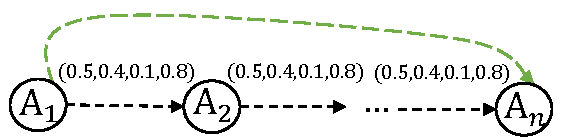
\includegraphics[width=0.4\textwidth]{img/discount/rs2.pdf}
    \caption{Generic referral path with the same numerical opinion for each edge}
    \label{fig:rs2}
\end{figure}

\begin{figure}
    \centering
    \begin{subfigure}{0.45\textwidth}
        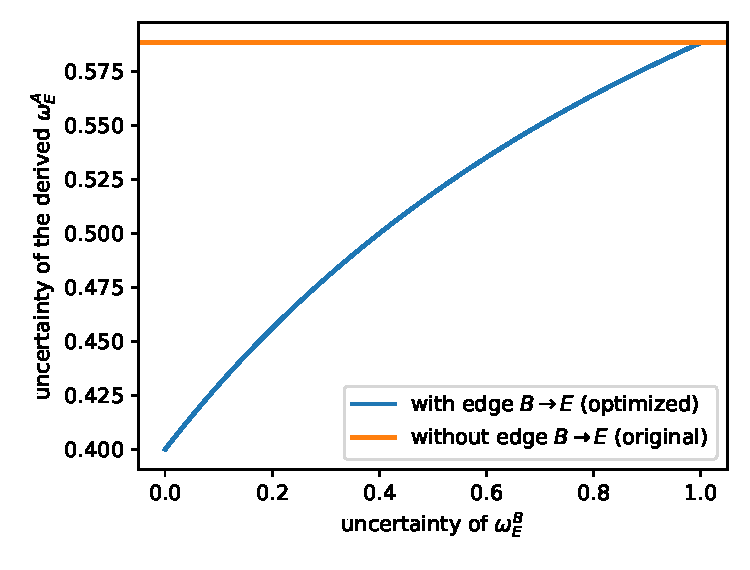
\includegraphics[width=\textwidth]{img/dspg/evalCum.pdf}
        \caption{Impact of edge $B \rightarrow E$ using cumulative fusion}
    \end{subfigure}
    \hfill
    \begin{subfigure}{0.45\textwidth}
        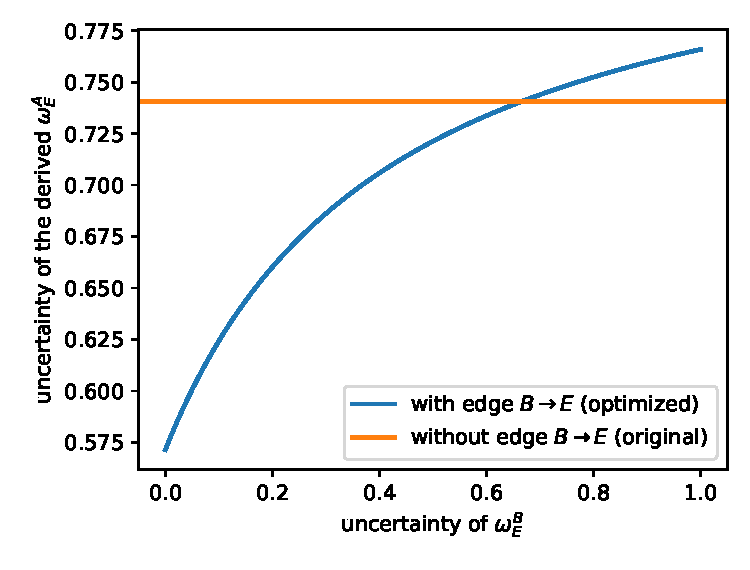
\includegraphics[width=\textwidth]{img/dspg/evalAvg.pdf}
        \caption{Impact of edge $B \rightarrow E$ using averaging fusion}
    \end{subfigure}
    \caption{Impact of retaining edge $B \rightarrow E$ on the uncertainty of the final derived opinion under different fusion operators}
    \label{fig:uncertainty_curves}
\end{figure}

\paragraph{Cumulative Fusion.}

When cumulative fusion is used, including the additional edge $\omega_E^B$ consistently lowers the uncertainty of the final opinion $\omega_A^E$, even when $\omega_E^B$ is highly uncertain. This behavior reflects the cumulative nature of the operator: additional independent evidence, even if partially uncertain, reduces overall uncertainty. Discarding $\omega_E^B$ therefore removes useful supporting evidence and leads to uniformly higher uncertainty.

\paragraph{Averaging Fusion.}
With averaging fusion, the effect depends on the uncertainty level of $\omega_E^B$. When $u(\omega_E^B)$ is small, retaining the edge reduces the final uncertainty. As $u(\omega_E^B)$ approaches $1$, the contribution of $\omega_E^B$ becomes increasingly detrimental, eventually producing higher uncertainty than the case where the edge is removed. This illustrates that averaging fusion is more sensitive to low-quality inputs. However, eliminating structurally valid edges still discards potentially informative trust paths.

These results confirm the practical relevance of the optimized DSPG synthesis criteria. Although minimizing uncertainty alone is not a sufficient objective, preserving structurally valid trust edges ensures that all meaningful trust evidence is retained. The optimized criteria therefore improve inference robustness by preventing premature information loss while maintaining structural correctness.


\subsection{Evaluation of \acs{DSPG} Analysis }
\todo[inline]{Evaluate the Time}
\subsection{Evaluation of Referral-Edge Trust Discounting}
\label{subsec:eval_referral}

\begin{figure}
    \centering
    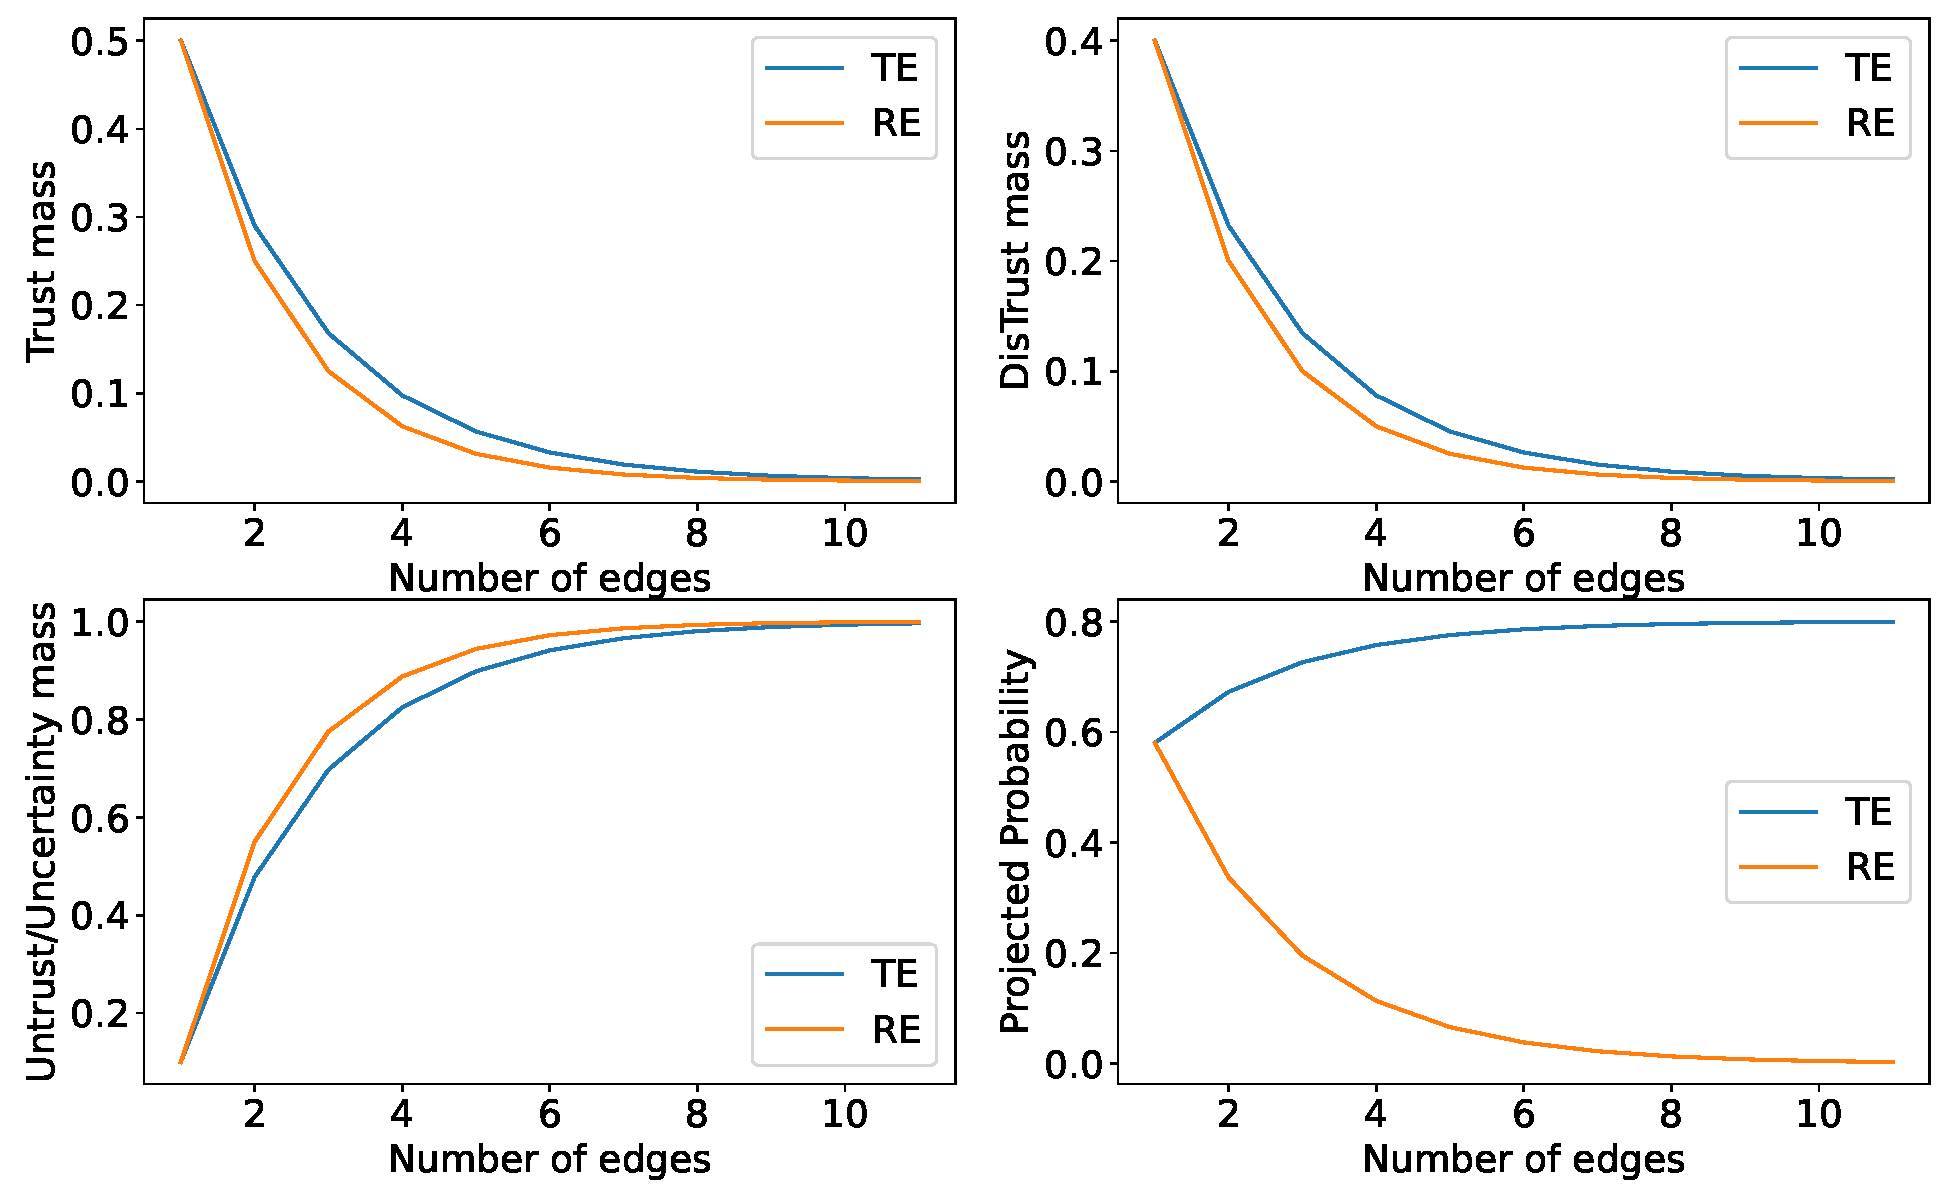
\includegraphics[width=0.8\textwidth]{img/discount/eval.pdf}
    \caption{Comparison of discounting referral edges using Two-Edge Path operator (TE) and the new operator, Referral-Edge Path (RE) on a transitive graph consisting in a varying number of referral edges with all edges having the same trust opinion: (0.5, 0.4, 0.1, 0.8) as depicted in~\cref{fig:rs2}. }
    \label{fig:eval}
    \vspace*{-0.4cm}
\end{figure}


In Section~\ref{sec:meth}, we analytically proved the equivalence between two methods for computing trust over multi-edge referral paths: 

\begin{itemize}
    \item Method 1: Multi-Edge Path discounting.
    \item Method 2: Referral-Edge Path discounting followed by Two-Edge Path discounting.
\end{itemize}

The goal of this section is to numerically validate this equivalence and to illustrate the limitations of the classical Two-Edge Path operator when applied to multiple referral edges.

\subsubsection{Comparison with Multi-Edge and Two-Edge Operators}

We consider the STN depicted in Figure~\ref{fig:rs1}. The following experimental setups are evaluated:

\begin{description}
    \item[Setup 1] Computation of $\omega_X^A$ using the Multi-Edge Path operator (Method 1).
    \item[Setup 2] Computation of $\omega_X^A$ using Referral-Edge Path operator followed by Two-Edge Path operator (Method 2).
    \item[Setup 3] Computation of $\omega_X^A$ using the Two-Edge Path operator applied twice.
\end{description}

\paragraph{Validation of Analytical Equivalence}

Using the opinion values from Figure~\ref{fig:rs1}, we obtain:

\begin{enumerate}
    \item Setup 1:
    \[
    \omega_X^A 
    =
    [\omega^A_B; \omega^B_C] \otimes_{ME} \omega^C_X
    =
    (0.14, 0.07, 0.79)
    \]

    \item Setup 2:
    \[
    \omega_X^A
    =
    (\omega_B^A \otimes_{RE} \omega_C^B) \otimes_{TE} \omega_X^C
    =
    (0.14, 0.07, 0.79)
    \]
\end{enumerate}

The identical numerical results confirm the analytical equivalence established earlier. The proposed operator therefore preserves the semantics of the Multi-Edge Path operator when used in combination with Two-Edge discounting.

\paragraph{Demonstrating the Limitation of Two-Edge Discounting}

We now apply Setup 3, where the Two-Edge Path operator is used to discount two referral edges:

\[
\omega_X^A
=
(\omega_B^A \otimes_{TE} \omega_C^B) \otimes_{TE} \omega_X^C
=
(0.22, 0.11, 0.67)
\]

This result differs significantly from Setups 1 and 2. 

This numerical inconsistency confirms that the Two-Edge Path operator cannot be applied iteratively to referral edges. It lacks associativity and does not preserve projected probability multiplicativity over referral chains. This validates the necessity of the proposed Referral-Edge Path operator.

\subsubsection{Evaluation on Generic Referral Chains}

To further analyze operator behavior, we consider the generic referral path illustrated in Figure~\ref{fig:rs2}. The path contains only referral edges, each assigned the identical opinion:

\[
(0.5, 0.4, 0.1, 0.8)
\]

The number of intermediate nodes varies, allowing us to observe how belief, disbelief, uncertainty, and projected probability evolve as the referral path length increases.

We compare:

\begin{itemize}
    \item Referral-Edge Path operator (RE)
    \item Two-Edge Path operator (TE)
\end{itemize}

The cumulative expressions are:

\begin{align}
\omega^{A_1}_{A_n}
&=
((\omega^{A_1}_{A_2} \otimes_{RE} \dots )
\otimes_{RE}
\omega^{A_{n-2}}_{A_{n-1}})
\otimes_{RE}
\omega^{A_{n-1}}_{A_n}
\label{eq:RE_eval}
\end{align}

\begin{align}
\omega^{A_1}_{A_n}
&=
((\omega^{A_1}_{A_2} \otimes_{TE} \dots )
\otimes_{TE}
\omega^{A_{n-2}}_{A_{n-1}})
\otimes_{TE}
\omega^{A_{n-1}}_{A_n}
\label{eq:TE_eval}
\end{align}

Since the Two-Edge operator is not associative, different grouping strategies yield different results. For consistency, we follow a fixed left-to-right grouping.

\paragraph{Observed Behavior}

Figure~\ref{fig:eval} illustrates the evolution of belief, disbelief, uncertainty, and projected probability as the path length increases.

For both operators:

\begin{itemize}
    \item Belief decreases.
    \item Disbelief decreases.
    \item Uncertainty increases.
\end{itemize}

However, their projected probability behaviors differ fundamentally:

\begin{itemize}
    \item For the Referral-Edge operator, projected probability decreases toward zero as the path length increases.
    \item For the Two-Edge operator, projected probability increases toward the base rate value $0.8$.
\end{itemize}

\paragraph{Analytical Explanation}

From the definitions of the operators:

For Two-Edge discounting:
\[
b^{[A;B]}_C = P_B^A b_C^B
\]

For Referral-Edge discounting:
\[
b^{[A;B]}_C = b_B^A b_C^B
\]

Since the projected probability satisfies:
\[
P_B^A = b_B^A + a_B^A u_B^A \geq b_B^A,
\]

the Two-Edge operator produces larger belief and disbelief components than the Referral-Edge operator. Consequently, the uncertainty mass for Two-Edge discounting is smaller.

This explains why the uncertainty curve for RE lies above TE in Figure~\ref{fig:eval}.

\paragraph{Impact of Base Rate Sensitivity}

Although the Referral-Edge operator produces higher uncertainty, it prevents excessive sensitivity to the base rate.

Under Two-Edge discounting, as uncertainty approaches one and belief and disbelief approach zero, the projected probability converges toward the base rate of the final edge. In this example, this leads to convergence toward $0.8$ for long paths.

This behavior masks the structural weakening of long referral chains.

In contrast, the proposed operator maintains multiplicative projected probability decay. As the number of referral edges increases, the projected probability decreases toward zero. This aligns with the intuition that long referral chains should represent weaker trust.

\paragraph{Interpretation}

The proposed Referral-Edge Path operator therefore satisfies three essential properties:

\begin{enumerate}
    \item Associativity over referral chains.
    \item Preservation of projected probability multiplicativity.
    \item Reduced sensitivity to base rate dominance.
\end{enumerate}

These properties make it structurally and probabilistically coherent for modeling transitive trust in Subjective Trust Networks.


\subsection{End-to-End Evaluation of the Complete \acs{TNA-SL} Framework}
\label{subsec:eval_pipeline}
\section{Summary \& Conclusions}
\label{sec:summary_tnsl}

\chapter{\acf{PaTAS}}
\label{chap:ovl}
The previous chapters established the conceptual and methodological foundations for trust assessment in general and particularly in \ac{ML} systems. In particular, \cref{chap:Trust_method} introduced a general evidence-based methodology for trust evaluation, while \cref{chap:tnasl} improved the graph-based reasoning mechanisms required to compute trust expressions. Building on these foundations, this chapter introduces the \emph{\acf{PaTAS}}, a system architecture designed to operationalize the proposed methodology in \ac{ML} pipelines. \ac{PaTAS} provides a scalable and modular framework for performing trust assessment throughout both training and inference, starting from the training dataset. The system enables the evaluation of \ac{NN} outputs in parallel with their inference by allowing different trust sources and reasoning components to be processed independently, without impacting the standard \ac{NN} inference process. This design allows efficient evaluation of trust in complex \ac{NN} systems where multiple evidence streams must be combined. The concepts presented in this chapter build upon previous publication. In particular, the architecture and core reasoning principles are derived from the work presented in~\cite{patas}, currently under review at the \emph{Elsevier Knowledge Based Systems}.

\section{Introduction}

The analysis presented in the Related Work \cref{sec:gap_summary} highlights a fundamental limitation in existing approaches to uncertainty and trust in \ac{NN} systems. While a wide range of methods have been proposed to quantify uncertainty at different levels, no unified framework simultaneously provides (i) an explicit, evidence-based representation of trust, (ii) the assessment of dataset trustworthiness during training, and (iii) a consistent propagation of trust from data to model parameters and from inputs to predictions.

Classical probabilistic and Bayesian approaches offer rigorous tools for modeling uncertainty, but they do not represent trust as a structured and composable construct. Conversely, \ac{SL} provides a principled calculus for reasoning about belief, disbelief, and uncertainty, as well as mechanisms for trust transitivity and source credibility. However, its application to \ac{NN} systems remains limited, both in terms of pipeline integration and computational realization. In particular, existing approaches do not provide a framework capable of integrating heterogeneous trust sources and propagating trust consistently across the different stages of the learning pipeline.

Furthermore, current uncertainty-aware \ac{NN} methods are typically confined to specific levels of abstraction. Model-based approaches, such as \acp{BNN}~\cite{neal1996bayesian} and deep ensembles~\cite{https://doi.org/10.1002/widm.1249}, capture parameter uncertainty but do not account for dataset credibility. Input-level propagation methods model observation uncertainty at inference time, yet they do not incorporate the reliability of the training dataset.

Existing trust-oriented approaches remain similarly limited in scope. For instance, DeepTrust~\cite{10.3389/frai.2020.00054} proposes a mechanism to leverage training dataset trustworthiness to assess model-level trust. However, such approaches are restricted to the training phase and do not extend to inference-time trust assessment, where predictions must be evaluated on a per-input basis.

To address these limitations, this chapter introduces the \emph{\acf{PaTAS}}, a system architecture designed to operationalize a unified trust assessment framework across the entire pipeline. \ac{PaTAS} enables the integration of multiple trust sources, including dataset reliability, model parameters, and input uncertainty, into a coherent and composable evaluation process.

A key feature of \ac{PaTAS} is its ability to perform trust assessment in parallel with standard \ac{NN} computations. By decoupling trust reasoning from the prediction process, the system allows trust to be computed alongside model outputs without modifying the internal structure of the \ac{NN}. This design ensures scalability, modularity, and compatibility with existing \ac{ML} systems.

This chapter focuses on the architectural design of \ac{PaTAS}, including its core components and its integration within \ac{ML} pipelines. The technical mechanisms underlying trust propagation and computation are presented in the following chapter.




\section{\ac{PaTAS} General Description}

\ac{PaTAS} is a framework designed to assess and propagate trust throughout the pipeline of a \ac{NN}. It operates in parallel with the standard neural architecture and maintains a corresponding trust flow that mirrors the \ac{ML} pipeline. This design enables trust to be evaluated continuously, from the construction of the training dataset to inference-time predictions.

The trust of the \ac{NN} output computed by \ac{PaTAS} is derived from two complementary sources:
\begin{enumerate}
    \item \textbf{Trust in model parameters}, obtained from the trustworthiness of the training dataset. This includes both the reliability of input features and the credibility of labels used during training.
    \item \textbf{Trust in inference inputs}, corresponding to the reliability of the input features provided at prediction time.
\end{enumerate}

By combining these two sources, \ac{PaTAS} enables the computation of trust in model outputs. This is particularly important as a reliable input does not necessarily guarantee a reliable prediction. For instance, an input \(x\) may be accurate and trustworthy (i.e., high trust score \(T_x\)), while the corresponding prediction \(y'\) may still be unreliable due to biased, noisy, or poorly calibrated model parameters \(\theta\) (i.e., low trust score \(T_{y'}\)). \ac{PaTAS} explicitly captures this distinction by evaluating trust across all stages of the pipeline.

Importantly, the notion of trust considered in \ac{PaTAS} is \emph{property-dependent}. Trust is always defined with respect to a specific property of interest, such as accuracy, bias, fairness, or any user-defined criterion. The assessment performed at the data level determines the nature of the trust that is propagated throughout the system. For instance, if the training dataset is evaluated with respect to accuracy, the resulting trust reflects the confidence in the correctness of predictions. Similarly, if the assessment targets bias or representativeness, the propagated trust captures the reliability of the model with respect to these properties. As a result, \ac{PaTAS} provides a flexible framework in which different trust dimensions can be analyzed independently or jointly, depending on the property under consideration.

A key design principle of \ac{PaTAS} is that it operates externally to the \ac{NN}. Rather than modifying the internal computations of the model, \ac{PaTAS} performs trust reasoning alongside the standard forward and backward passes. This non-intrusive approach preserves the original predictive behavior of the \ac{NN}, avoids additional computational overhead within the model, and ensures compatibility with existing architectures.

\marginpar{Workflow Overview}
The overall workflow of \ac{PaTAS} is illustrated in \cref{fig:ovvwptas}. The process begins at the data level, where multiple data providers contribute to a data warehouse. The collected data undergoes preprocessing steps, including data cleaning, labeling and more, resulting in the construction of the training dataset.

\ac{PaTAS} first performs a \emph{training dataset trustworthiness assessment}, where evidence from the dataset is used to quantify the reliability of both input features and labels. This step produces trust scores associated with the training data, which are then used to derive trust in the model parameters during the training process.

Once the model is trained, \ac{PaTAS} enables \emph{trust propagation within the \ac{NN}}. During inference, the system receives a query from the user, which is processed by the \ac{NN} to generate a prediction. In parallel, \ac{PaTAS} evaluates the trustworthiness of the input and propagates it through the model, combining it with parameter trust to produce a trust score associated with the output.

Importantly, this trust computation is performed as a parallel function that does not interfere with the \ac{NN} inference. As shown in \cref{fig:ovvwptas}, the system produces both a prediction and an associated trust score, enabling the user to assess not only what the model predicts, but also how reliable that prediction is.

\begin{figure}
    \centering
    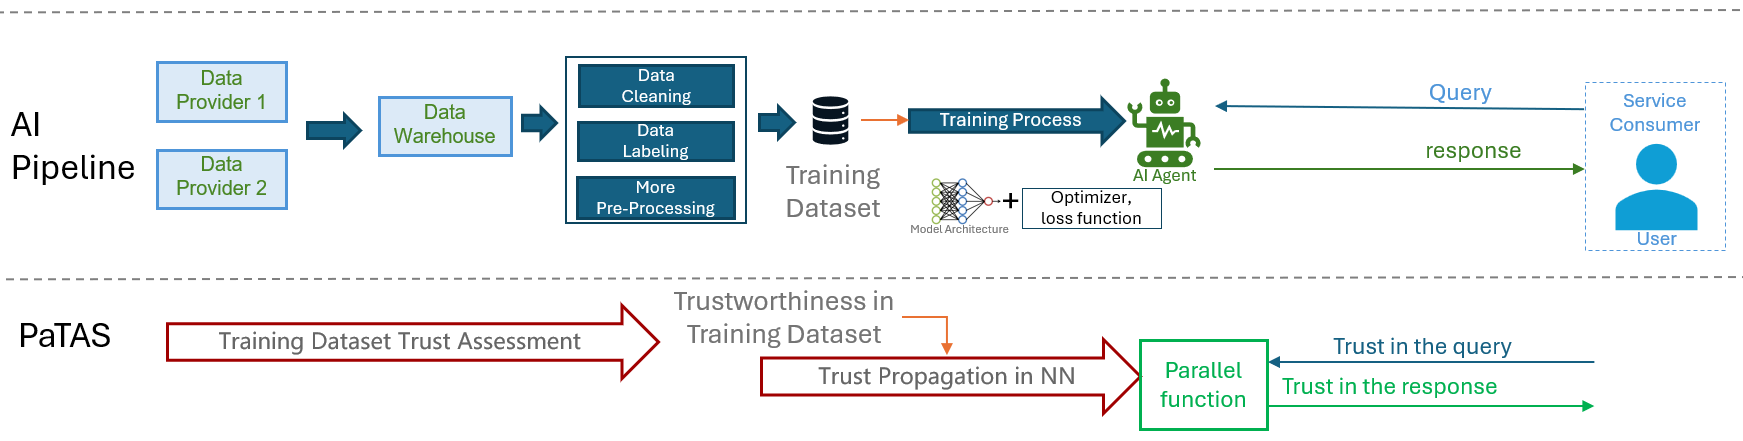
\includegraphics[width=\linewidth]{img/patas/overviewPTAS.png}
    \caption{PaTAS workflow - from dataset trustworthiness assessment to trust propagation during inference.}
    \label{fig:ovvwptas}
\end{figure}

\section{Functionalities}

\begin{figure}
    \centering
    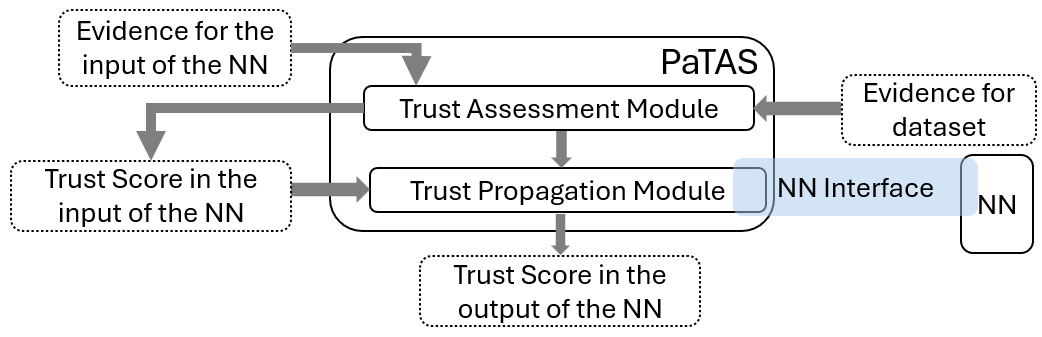
\includegraphics[width=\linewidth]{img/patas/end_to_end.png}
    \caption{Overview of the \acs{PaTAS} framework for end-to-end trust assessment in \ac{NN} pipelines.}
    \label{fig:patas_all}
\end{figure}

\subsection{Core Components}

The functionalities of \ac{PaTAS} are organized around two complementary components, as illustrated in \cref{fig:patas_all}. These components correspond to two fundamental aspects of trust assessment in \ac{ML} pipelines: (1) the evaluation of data trustworthiness, including both training datasets and input data at inference time, and (2) the propagation of trust through the \ac{NN}.

\paragraph{Trust Assessment Module} The first component focuses on the assessment of the trustworthiness of the training dataset and the input of the \ac{NN}. This assessment is \emph{property-dependent}, meaning that trust is quantified with respect to a specific property of interest, such as accuracy or bias. It relies on evidence extracted from the data, including the reliability of input features and the credibility of labels, in relation to the selected property. This process produces trust scores associated with the training samples (and input data in general), which are then used to derive trust in the learned model parameters. Consequently, the nature of the propagated trust directly depends on the property used during the assessment stage. This component establishes the foundation of trust for the entire pipeline.

\paragraph{Trust Propagation Module}
The second component is responsible for propagating trust through the \ac{NN}. It leverages the trust derived from the training dataset to assess the reliability of model parameters and combines it with the trust associated with input features at inference time. This component enables the computation of trust scores at different levels of abstraction, including neuron-level, layer-level, and output-level trust. Together, these two components form a unified framework for end-to-end trust assessment.

\subsection{Operational Phases}

The behavior of \ac{PaTAS} can be described through three operational phases, corresponding to different stages of the \ac{NN} lifecycle.
\begin{enumerate}
    \item \textbf{Dataset Trust Assessment Phase:} In the first phase, \ac{PaTAS} evaluates the trustworthiness of the training dataset. This involves analyzing the quality of input features and labels to produce trust scores associated with the training data. These scores serve as the initial source of trust for subsequent stages.
    \item \textbf{Training Propagation Phase:} In the second phase, the trust derived from the training dataset is propagated through the \ac{NN} during the training process. This phase enables the estimation of trust in the learned model parameters, reflecting how the quality of the data influences the reliability of the model.
    \item \textbf{Inference Propagation Phase:} In the third phase, \ac{PaTAS} operates during inference to assess the trustworthiness of individual predictions. Trust associated with the input is propagated through the network and combined with parameter trust to produce a trust score for the output. This enables per-instance trust evaluation and supports informed decision-making based on both predictions and their associated reliability.
\end{enumerate}

Notably, the last two phases correspond to trust propagation mechanisms, while the first phase provides the foundational trust assessment derived from the training dataset.

\section{Summary \& Conclusions}

This chapter introduced \ac{PaTAS}, a modular and scalable framework designed to operationalize trust assessment in \ac{ML} pipelines.

Building upon the general trust assessment methodology and the graph-based reasoning mechanisms presented in previous chapters, the two main components of \ac{PaTAS} provide a practical system for evaluating and propagating trust throughout both training and inference.

The framework is structured around two main components: the assessment of data trustworthiness and the propagation of trust through the \ac{NN}. These components enable the integration of multiple trust sources, including data reliability, label credibility, and input uncertainty, into a unified and composable trust evaluation process. By operating in parallel with the \ac{NN}, \ac{PaTAS} ensures that trust assessment remains non-intrusive and does not interfere with the model’s predictive behavior.

Furthermore, the definition of distinct operational phases allows \ac{PaTAS} to capture the dynamic nature of trust across the learning lifecycle, from dataset construction to inference-time prediction. This enables both global and per-instance trust evaluation, addressing key limitations of existing approaches that are confined to isolated stages or specific types of uncertainty.

Overall, \ac{PaTAS} constitutes the operational layer of the proposed trust assessment framework, bridging the gap between theoretical trust modeling and practical AI system deployment. The next chapter builds upon this architecture by formalizing the mechanisms underlying trust propagation within \acp{NN}, including the operators and computational processes that enable consistent and scalable trust reasoning.
% =====================================================================
%  Chapter 6 -- Assessment of AI Training Datasets Trustworthiness
%
%  Revised 2026-09 following F. Kargl's review of 2026-06-24 (73 comments,
%  see reviews/ch06-fk-review-2026-06-24.md). Main changes:
%   * scope / contributions / roadmap added to the introduction;
%   * Sec. 6.2 re-grounded in dataset examples instead of re-introducing Ch. 2;
%   * Phase I = structure (tree + trust-source catalogue), Phase II =
%     quantification (metric -> evidence -> opinion, hyperparameters);
%   * every application states its purpose / research question, introduces
%     its dataset, and closes with "what this example showed";
%   * terminology unified: trust source (not metric), belief/disbelief (b,d,u).
%
%  Labels follow chap6:* / sec:* / fig:* / tab:* / eq:* conventions.
% =====================================================================

\chapter{Assessment of AI Training Datasets Trustworthiness}
\label{chap:dataset-trust}
\acresetall
The previous chapter presented the overall architecture of \ac{PaTAS}, highlighting its two main components: (i) the Trust Assessment Module, which assesses the trustworthiness of the training dataset and of the input of the \ac{NN}, and (ii) the Trust Propagation Module, which propagates trust through the model, from the training data to the learned parameters and from the input to the output via these parameters. This chapter focuses on the first component, the trust assessment module. The underlying ideas were initially explored in the paper presented at the BIAS Workshop at ECML PKDD~\cite{10.1007/978-3-032-19096-3_17} and further developed in the paper on labeling accuracy presented at the TRUST-AI Workshop of ECAI~\cite{trust-aidatatrust}. In this dissertation, these contributions are unified and extended into a single framework for assessing the trustworthiness of training datasets.

% --------------------------------------------------------------
\section{Introduction}
\label{sec:dataset-trust:intro}

The chapter is organized around three observations. First, \emph{the trustworthiness of a training dataset is not a scalar.} Different trustworthiness properties such as fairness, correctness, representativeness, privacy compliance, and robustness to leakage require different types of evidence, different evaluation granularities, and different aggregation rules. Collapsing them into a single quality score, or applying the same metric, the same threshold, and the same aggregation rule across all of them, hides exactly the information that should drive downstream decisions: which property is at risk, at which stage of the lifecycle.

Second, \emph{properties live at different levels of the data}. Some properties are only meaningful at the \textbf{dataset level} (e.g., class balance, coverage). Others are intrinsically \textbf{per-entry} (e.g., label correctness) or \textbf{per-feature} (e.g., the reliability of an individual sensor channel).

Third, \emph{evidence about trustworthiness is rarely complete}. Training datasets are typically constructed through multi-stage lifecycles in which documentation, metadata, and direct observations are partial, sometimes contradictory, and often unavailable for historical pipelines. The framework must therefore distinguish \emph{low support} from \emph{no support}, which is exactly what \aclu{SL} offers and what scalar quality scores cannot.

\paragraph{Scope.}
The object of this chapter is the \emph{training dataset} $\dataset$ of a \ac{NN}: the collection of entries (rows, images, records) and their labels that the model is trained on. The framework produces trust opinions about $\dataset$, or about parts of it, with respect to a stated property. Inputs presented to the model at inference time are \emph{not} the object of this chapter. They are mentioned only because the entry- and feature-level trust sources introduced here apply unchanged to a single input, which is how \cref{chap:patas} obtains an input-level trust opinion; that use is discussed in \cref{sec:dataset-trust:summary}.

\paragraph{Contributions.}
The chapter makes the following contributions.
\begin{enumerate}
  \item A \emph{three-axis design space} $(\propP, \propS, \propG)$ (property, lifecycle stage, granularity) that turns the question ``is this dataset trustworthy?'' into a well-posed trust proposition, and a \emph{lifecycle decomposition} of composite propositions into stage-level propositions (\cref{sec:dataset-trust:framework:design-space,sec:dataset-trust:framework:phase1}).
  \item A \emph{catalogue of trust sources} (\cref{tab:dataset-trust:catalogue}): diagnostics organized by lifecycle stage, risk category, property and granularity, from which the leaves of a trust expression are selected. The catalogue is a starting point and is meant to be extended.
  \item A \emph{quantification procedure} that turns the value returned by a trust source into evidence, and evidence into a subjective opinion, with explicit hyperparameters and guidance on how to set them (\cref{sec:dataset-trust:framework:phase2}).
  \item \emph{Cross-granularity composition} mechanisms that let feature- or entry-level evidence support entry- or dataset-level propositions (\cref{sec:dataset-trust:formal:granularity}).
  \item Three instantiations of the framework: a multi-stage \emph{illustration} on the \acs{COMPAS} dataset (\cref{sec:dataset-trust:applications:compas}) and two \emph{evaluations}, on class balance with \ac{GTSRB} (\cref{sec:dataset-trust:applications:gtsrb}) and on labeling accuracy with CIFAR-10H (\cref{sec:dataset-trust:applications:cifar10h}), in which the trust opinions are checked against known ground truth or downstream model behavior.
\end{enumerate}

\paragraph{Roadmap.}
\cref{sec:dataset-trust:uncertainty} asks what the sources of uncertainty concretely mean for a training dataset. \cref{sec:dataset-trust:framework} presents the methodology: the design space, then the three phases of the General Methodology of \cref{chap:Trust_method} restated for datasets, with Phase~I fixing the \emph{structure} of the assessment and Phase~II its \emph{quantification}. \cref{sec:dataset-trust:framework:applications-overview} explains how the three applications were selected and what each is meant to show; \cref{sec:dataset-trust:applications:compas,sec:dataset-trust:applications:gtsrb,sec:dataset-trust:applications:cifar10h} present them. \cref{sec:dataset-trust:summary} summarizes the chapter, discusses its limitations and explains how its outputs feed the Trust Propagation Module of \cref{chap:patas}.

\paragraph{Terminology.}
Throughout the chapter, a \emph{trust source} is, as in \cref{chap:Trust_method}, anything that provides evidence for a trust proposition about the dataset. In this chapter it is typically a diagnostic computed on the data (e.g., a distribution gap, an entropy), but it can also be an audit of the dataset's documentation, or a score derived from the responses of human annotators. We use the word \emph{metric} only for the raw numerical value a trust source returns. Opinions are written $\omega = (b, d, u)$ with belief $b$, disbelief $d$ and uncertainty $u$, following \cref{chap:rw}; the base rate is $a = 0.5$ unless stated otherwise. As everywhere in this dissertation, since the propositions assessed are trust propositions, \emph{belief} and \emph{trust} are used interchangeably, and so are \emph{disbelief} and \emph{distrust} (\cref{chap:Trust_method}).

% --------------------------------------------------------------
\section{Sources of Uncertainty in Training Datasets Assessment}
\label{sec:dataset-trust:uncertainty}

\cref{chap:rw} explained why classical probability conflates the randomness of a variable with the analyst's ignorance about it, and why conflicting and missing evidence call for an evidence-based formalism such as \aclu{SL}. Trust assessment usually distinguishes four sources of uncertainty: randomness, system complexity, conflicting evidence and lack of evidence; only the first is adequately captured by probability alone. This section does not re-introduce these notions; it asks what each of them concretely looks like when the object under assessment is the training dataset of a \ac{NN}, and why that matters for the design of the framework. \cref{tab:dataset-trust:uncertainty-examples} summarizes the mapping.

\begin{table}[!htbp]
  \centering
  \small
  \renewcommand{\arraystretch}{1.2}
  \begin{tabular}{@{}p{2.6cm}p{5.4cm}p{5.4cm}@{}}
    \toprule
    \textbf{Source} & \textbf{In a training dataset} & \textbf{Consequence for the assessment} \\
    \midrule
    Randomness & A sensor-consistency score fluctuates across repeated measurements; a subsampled class distribution varies across draws. & Variability of the \emph{value} returned by a trust source; well handled by probability, and absorbed by the evidence counts. \\
    System complexity & Data merged from several sites, devices or years; a pre-processing pipeline whose steps are only partly documented. & The analyst cannot isolate which stage caused a defect; the opinion must be able to carry uncertainty about a stage rather than a verdict. \\
    Conflicting evidence & Group representation looks balanced but an audit reveals undocumented exclusion criteria; \ac{IAA} is high while labels are biased against a minority group. & Belief and disbelief must be kept as \emph{separate} masses; averaging them into one score hides the conflict. \\
    Lack of evidence & No annotation guidelines are available; the reference population used for sampling is unknown; a stage has no diagnostic at all. & Absence of evidence must show up as uncertainty, not as ``no problem found''. \\
    \bottomrule
  \end{tabular}
  \caption{The four sources of uncertainty in trust assessment instantiated on a training dataset.}
  \label{tab:dataset-trust:uncertainty-examples}
\end{table}

\subsection{Fundamental Sources of Uncertainty}
\label{sec:dataset-trust:uncertainty:sources}

\subsubsection{Uncertainty Addressable by Classical Probability Theory}
\label{sec:dataset-trust:uncertainty:probability}
Randomness appears in a dataset assessment when the trust source itself is governed by a stochastic process. A sensor-consistency score computed on repeated measurements of the same physical quantity varies with sensor noise; a class-balance statistic computed on a random subsample varies across draws. When the process generating the value is well specified and enough observations are available, this variability can be characterized by a distribution, and it is naturally absorbed by the evidence counts of \cref{chap:Trust_method}: more observations mean more evidence and less uncertainty.

What probability alone does not offer is a way to represent that (i) the diagnostic itself may be unreliable, (ii) too few observations may be available for residual uncertainty to be ignored, and (iii) two diagnostics may disagree. In dataset construction these situations are the norm rather than the exception.

\subsubsection{Uncertainty Requiring Evidence-Based Modeling}
\label{sec:dataset-trust:uncertainty:evidence}

\paragraph{System complexity.}
A dataset is the product of several interacting processes: a sampling strategy, one or more collection protocols, an annotation workflow and a pre-processing pipeline, often executed by different actors at different times. Consider a driving dataset assembled from vehicles of several \acp{OEM}, recorded over three years with two generations of cameras and labeled by two annotation vendors. If the model later under-performs on a class, the analyst can usually not tell whether the cause is sampling (the class was rare on the routes driven), collection (the older camera blurs it), annotation (one vendor mislabels it) or pre-processing (an aggressive de-duplication step removed most of its instances). Complexity is thus an epistemic condition: the analyst's knowledge of \emph{which} stage holds is incomplete, and the framework must allow each stage to carry its own uncertainty. Decomposing the assessment along the lifecycle, and reasoning on the resulting graph with \ac{SL} (\cref{chap:tnasl}), is the response to this condition.

\paragraph{Conflicting and incomplete evidence.}
Conflicting evidence occurs when two trust sources about the same stage disagree: a group-representation ratio indicates balanced demographic coverage while a documentation audit reveals that a subgroup was excluded at collection time; or high \ac{IAA} coexists with a systematic label bias affecting a minority group (annotators agree with each other, but agree on the wrong label). Lack of evidence occurs when a stage simply has no diagnostic: annotation guidelines are not available, the reference population used for sampling is unknown, or the pre-processing steps of a historical dataset were never documented. Collapsing all signals into a single probability either hides the disagreement or silently treats absence of evidence as evidence of absence. \aclu{SL} avoids both failures by keeping belief, disbelief and uncertainty as distinct masses.

These sources co-occur in practice: a real training dataset is assembled through a multi-stage lifecycle involving heterogeneous actors, tools and governance regimes, so randomness, complexity, conflicting signals and missing information are simultaneously present. The framework presented next therefore relies on \ac{SL} as its formalism. \ac{SL} alone, however, does not say \emph{which} propositions to formulate, \emph{which} trust sources to consult, or \emph{how} to combine them across the lifecycle. Those choices are the role of the framework.

% --------------------------------------------------------------
\section{A Methodology for Trust Assessment of Training Datasets}
\label{sec:dataset-trust:framework}

This section presents the proposed framework. Rather than producing a single score, dataset trustworthiness is represented as a structured and property-dependent trust assessment that explicitly accounts for incomplete, conflicting, or missing information.
\label{sec:dataset-trust:framework:principles}
The framework is built on three design principles.
\begin{enumerate}
  \item \textbf{Property-dependent assessment.} Trustworthiness is always defined with respect to a specific property of interest. The same dataset may be highly trustworthy for one property and not for another, in line with the trust-proposition formalism introduced in \cref{chap:Trust_method}.
  \item \textbf{Lifecycle-based reasoning.} Dataset trustworthiness emerges from the correctness of the processes that produce and transform the data. The framework therefore decomposes evaluation along the four stages of the dataset lifecycle: \emph{sampling} (which population, time span and sources are covered), \emph{collection / measurement} (how raw values are acquired), \emph{annotation} (how labels are produced) and \emph{processing}. By \emph{processing} we mean the transformations applied to the data \emph{before} training: cleaning, de-duplication, feature selection, augmentation and synthetic generation.
  \item \textbf{Multi-granular evaluation.} Some properties are meaningful only at the level of the dataset as a whole (e.g., class balance), others at the level of individual entries (e.g., label correctness), and others at the level of individual features (e.g., the reliability of one sensor channel). The framework supports trust sources operating at any of these three granularities and provides aggregation mechanisms between them.
\end{enumerate}

\subsection{The Three-Axis Design Space}
\label{sec:dataset-trust:framework:design-space}

A trust assessment of a training dataset is specified by three choices, which together form the design space of the framework and are written as the tuple $(\propP, \propS, \propG)$:

\begin{itemize}
  \item $\propP$ --- the \textbf{property} being assessed (e.g., accuracy, fairness, representativeness, privacy compliance), or a composite of several of them;
  \item $\propS$ --- the \textbf{lifecycle stage(s)} from which evidence is drawn,
        \\
        $\propS \subseteq \{\textsc{sampling}, \textsc{collection},
        \textsc{annotation}, \textsc{processing}\}$;
  \item $\propG$ --- the \textbf{granularity} at which the property is
        meaningful,
        \\
        $\propG \in \{\textsc{dataset}, \textsc{entry},
        \textsc{feature}\}$.
\end{itemize}
\noindent $\propS$ is a set: an assessment may draw on evidence from a single stage or from all four, as the \ac{COMPAS} application does. Selecting $(\propP, \propS, \propG)$ instantiates a specific assessment problem.

\paragraph{Role of each axis.}
The property $\propP$ determines \emph{which trust sources are admissible and what their output means as evidence}. Each trust source in the catalogue of \cref{tab:dataset-trust:catalogue} is tagged with the property it informs, and only those matching $\propP$ may appear in the trust expression: a class-count histogram is evidence for ``$\dataset$ is representative'' (positive when the counts match a reference distribution, negative otherwise) but says nothing about ``$\dataset$ is privacy-compliant'', for which a \ac{PII} audit is the relevant trust source. The stage $\propS$ identifies the component of the pipeline whose correctness is questioned: in the notation $\mathcal{T}(E, \propP)$ of \cref{chap:Trust_method}, each stage (e.g., ``the sampling stage of $\dataset$'') is the trustee $E$ of one stage-level trust proposition. The granularity $\propG$ fixes the unit at which evidence is collected and therefore which trust sources (tagged $\dGran$, $\eGran$ or $\fGran$ in the catalogue) can be attached.

\paragraph{Decomposition order.}
A composite trust proposition such as ``$\dataset$ is trustworthy for training'' is decomposed by traversing the axes in a fixed order. The property is identified first (here, \emph{overall trustworthiness}, defined below as the conjunction of all catalogue properties). The proposition is then split along $\propS$ into one proposition per lifecycle stage (\cref{eq:dataset-trust:lifecycle-decomposition}). Within each stage, the analyst chooses the granularity at which evidence is available: ``the sampling stage is trustworthy'' might be supported by a dataset-level trust source about the class distribution and a feature-level one about coverage; ``the annotation stage is trustworthy'' by an entry-level trust source about per-item label correctness and a dataset-level one about systematic group-level label bias. Each leaf of the resulting expression is one trust source from \cref{tab:dataset-trust:catalogue}. This fixed traversal order is, in the dataset setting, the expression-generation phase of the General Methodology.

\begin{mdframed}[backgroundcolor=gray!10, linewidth=0pt]
\textbf{Example.} Consider assessing whether the annotation stage of dataset $\dataset$ is accurate ($\propP$ = accuracy, $\propS$ = \{annotation\}, $\propG$ = entry). The trust proposition is ``the labels of $\dataset$ are correct''. Each entry is an atomic proposition ``the label of entry $x$ is correct''. The trust source is \acf{IAA}: for each entry, the fraction of independent annotators who assigned the same label, which is evidence for the label being correct when several annotators agree and against it when they disagree. The per-entry opinions are then aggregated (\cref{sec:dataset-trust:formal:granularity}) into a dataset-level opinion on label accuracy. \cref{sec:dataset-trust:applications:cifar10h} instantiates exactly this cell of the design space.
\end{mdframed}

\subsection{Phase~I --- Expression Generation: Fixing the Structure}
\label{sec:dataset-trust:framework:phase1}
The three-axis design space lets us restate the three phases of the General Trust Assessment Methodology in dataset-specific language. Phase~I fixes everything that is \emph{structural}: which propositions appear in the trust expression, how they are combined, and which trust source sits at each leaf. Nothing is quantified yet.

\paragraph{Lifecycle decomposition.}
When the trust proposition is composite (e.g., ``$\dataset$ is trustworthy for training''), it is decomposed along the lifecycle axis $\propS$. Each stage becomes the trustee of a simpler trust proposition, and the overall trust is their conjunction:
\begin{equation}
\mathcal{T}(\dataset, \propP)
= \mathcal{T}_{\text{sampling}} \wedge \mathcal{T}_{\text{collection}}
  \wedge \mathcal{T}_{\text{annotation}} \wedge \mathcal{T}_{\text{processing}},
\label{eq:dataset-trust:lifecycle-decomposition}
\end{equation}
which, in terms of opinions, reads
\[
\omega_{\mathcal{T}(\dataset, \propP)} = \omega_{\mathcal{T}_{\text{sampling}}} \cdot \omega_{\mathcal{T}_{\text{collection}}} \cdot \omega_{\mathcal{T}_{\text{annotation}} } \cdot \omega_{\mathcal{T}_{\text{processing}}},
\]
where $(\cdot)$ is the \ac{SL} conjunction operator (\cref{chap:rw}). Conjunction is the right connective because a dataset with trustworthy annotation but compromised sampling is not trustworthy overall.

\paragraph{Stage-level propositions and their trust sources.}
Each stage-level proposition is supported by one or more trust sources, which all provide evidence for the \emph{same} proposition and are therefore combined with a fusion operator ($\oplus$, cumulative fusion in this thesis) rather than conjoined:
\begin{equation}
\omega_{\mathcal{T}_{\text{sampling}}}
= \omega_{\text{DG}} \oplus \omega_{\text{MCR}} \oplus \omega_{\text{GRR}}
  \oplus \omega_{\text{LTCI}} \oplus \dots,
\label{eq:dataset-trust:metric-aggregation}
\end{equation}
and analogously for the other stages. \cref{fig:trust_expression_tree_dataset} shows the resulting two-level tree for $\propP$ = overall trustworthiness. In the General Methodology the leaves of a trust expression are \acp{ATO}; here each leaf is the opinion obtained from one trust source, and the fused stage-level opinion is what plays the role of the \ac{ATO} in the higher-level expression.

\begin{figure}[!htbp]
\centering
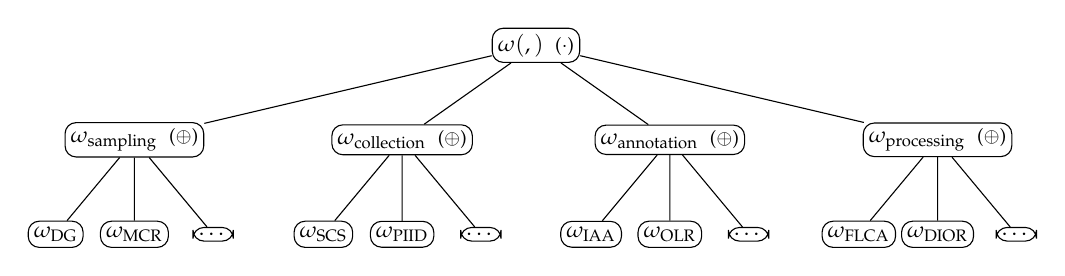
\begin{tikzpicture}[
  level distance=12mm,
  level 1/.style={sibling distance=34mm},
  level 2/.style={sibling distance=10mm},
  every node/.style={draw, rectangle, rounded corners, align=center,
                     inner sep=2pt, font=\footnotesize},
  edge from parent/.style={draw, thin}
]
\node {$\omega(\dataset, \propP)$ \;\scriptsize($\cdot$)}
  child { node {$\omega_{\text{sampling}}$ \;\scriptsize($\oplus$)}
    child { node {$\omega_{\text{DG}}$} }
    child { node {$\omega_{\text{MCR}}$} }
    child { node {$\dots$} }
  }
  child { node {$\omega_{\text{collection}}$ \;\scriptsize($\oplus$)}
    child { node {$\omega_{\text{SCS}}$} }
    child { node {$\omega_{\text{PIID}}$} }
    child { node {$\dots$} }
  }
  child { node {$\omega_{\text{annotation}}$ \;\scriptsize($\oplus$)}
    child { node {$\omega_{\text{IAA}}$} }
    child { node {$\omega_{\text{OLR}}$} }
    child { node {$\dots$} }
  }
  child { node {$\omega_{\text{processing}}$ \;\scriptsize($\oplus$)}
    child { node {$\omega_{\text{FLCA}}$} }
    child { node {$\omega_{\text{DIOR}}$} }
    child { node {$\dots$} }
  };
\end{tikzpicture}
\caption{Trust-expression tree for the running example $\propP$ =
  overall trustworthiness. The root combines the four stage-level opinions with conjunction
  ($\cdot$): the dataset is trustworthy only if every lifecycle stage is
  trustworthy. Each stage-level node fuses ($\oplus$) the opinions of the trust
  sources attached to it: they all provide evidence for the same stage-level
  proposition. Only two representative trust sources are shown per stage; the
  catalogue is given in \cref{tab:dataset-trust:catalogue}.}
\label{fig:trust_expression_tree_dataset}
\end{figure}

\paragraph{The trust-source catalogue.}
\cref{tab:dataset-trust:catalogue} is the catalogue from which the leaves of the tree are selected. It is organized by lifecycle stage and, within each stage, by \emph{risk category}: a named failure mode of that stage (e.g., temporal bias in sampling, measurement bias in collection). Each risk category is tagged with the property it threatens, so that the property axis $\propP$ can be used to filter the table, and each trust source is tagged with the granularity at which it naturally operates. The risk categories and the trust sources were assembled from the dataset-quality and bias literature: the bias taxonomy of Mehrabi et al.~\cite{10.1145/3457607} and of Suresh and Guttag~\cite{Suresh_2021} provided the risk categories, while the documentation practices of Datasheets~\cite{gebru2018datasheets} and Data Cards~\cite{Pushkarna2022DataCP} suggested which diagnostics are realistically available at each stage. The catalogue is deliberately \emph{not exhaustive}: it lists the trust sources considered in this thesis, and additional ones can be defined and selected when the framework is applied to a concrete system, as long as they are placed at a stage, a risk category and a granularity. \cref{fig:dataset-trust:overview} gives a graphical view of the same catalogue.

For the running example $\propP$ = overall trustworthiness, we define it as the conjunction of all properties in the catalogue: a dataset is trustworthy for training when it is representative, accurately measured and labeled, fair, privacy-compliant and free of leakage. Under this definition the whole catalogue is admissible, and the tree of \cref{fig:trust_expression_tree_dataset} is the \emph{maximal} decomposition. For a narrower $\propP$ the expression is the subtree obtained by pruning: an assessment of labeling accuracy retains only the annotation branch and, within it, only the trust sources tagged with \emph{accuracy}; a property defined exclusively at the entry level retains only the leaves whose granularity is $\eGran$.

\paragraph{Optional intermediate level.}
Between the stage level and the trust-source level, the framework can insert a third level grouping trust sources by risk category, as the layout of \cref{fig:dataset-trust:overview} suggests. This is useful when the analyst wants to require that a stage holds along several distinct risk axes \emph{simultaneously} (conjunction of risk categories, fusion within each). In this thesis we keep the two-level structure (stage $\to$ trust sources) for clarity; the three-level variant is a direct consequence of the framework and is left as an option for future instantiations. Similarly, when the way a stage is performed is itself described as a network of actors (several annotation vendors, several data providers), \acf{TNA-SL} (\cref{chap:tnasl}) can be used on the corresponding \aclu{STN} to expand the stage-level proposition into a finer expression.

\begin{figure}[!htbp]
  \centering
  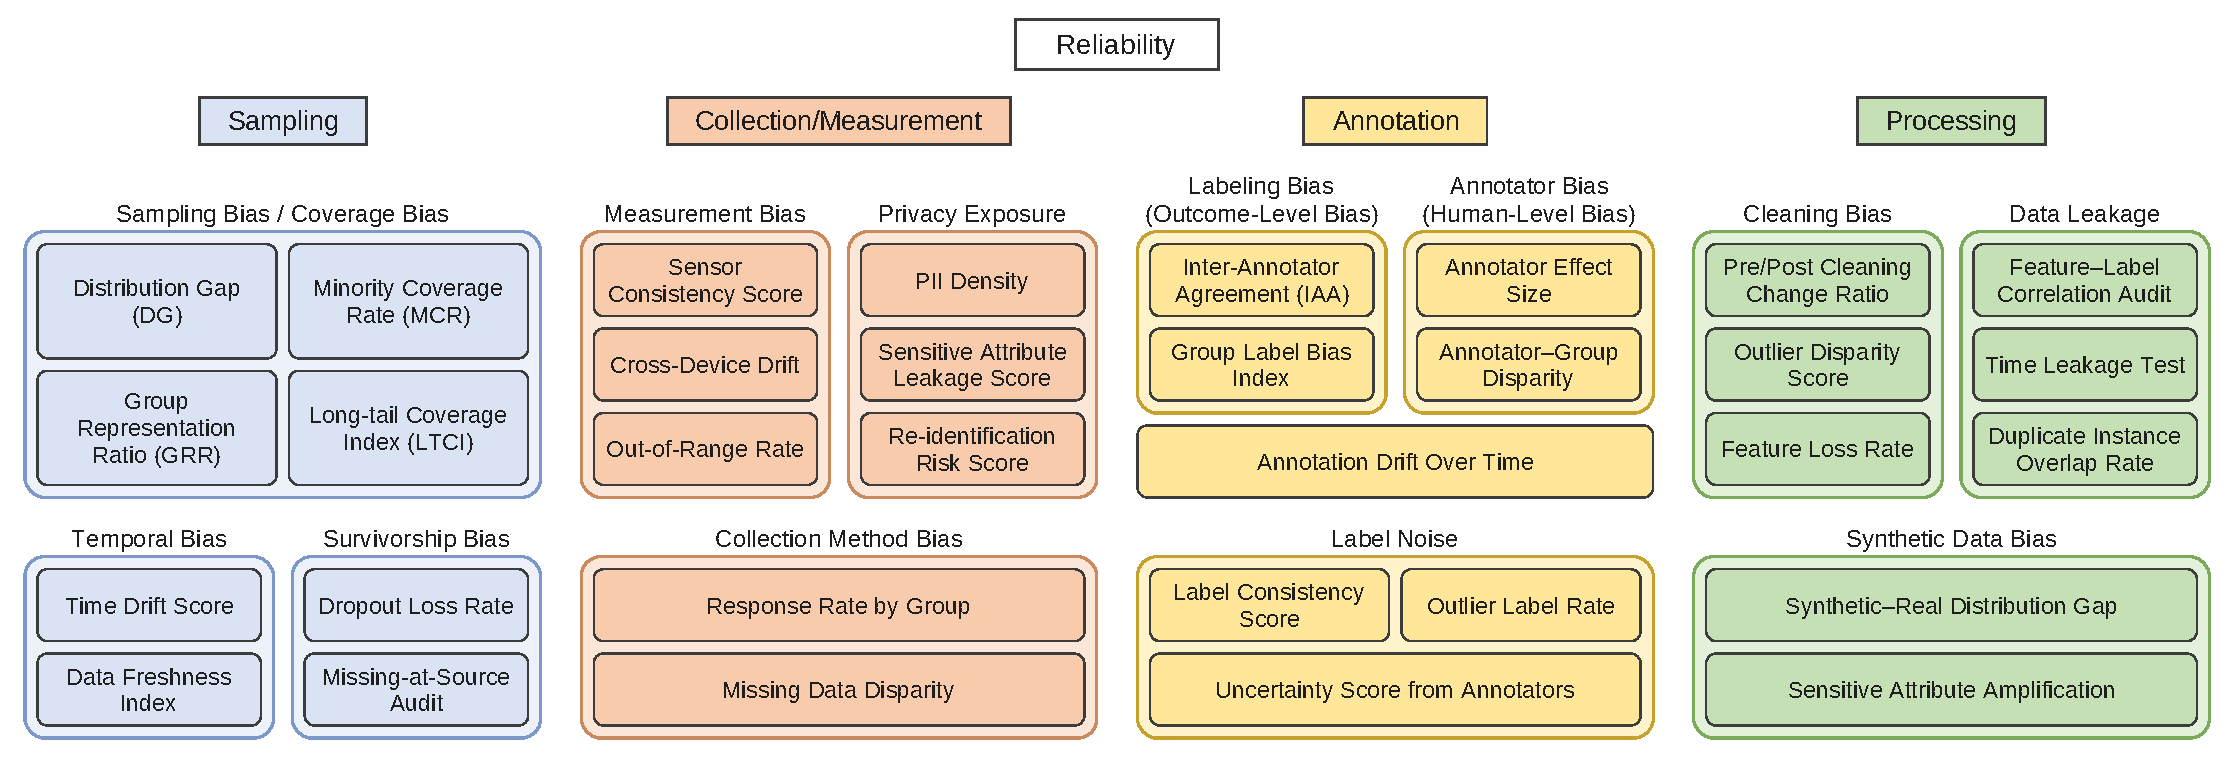
\includegraphics[width=\linewidth]{img/data/framework.pdf}
  \caption{Graphical view of the trust-source catalogue of \cref{tab:dataset-trust:catalogue}. Dataset trustworthiness is decomposed into lifecycle stages (sampling, collection, annotation, processing); within each stage, trust sources are grouped by risk category. The property each risk category informs is given in \cref{tab:dataset-trust:catalogue}. Evidence is aggregated under uncertainty using \ac{SL}.}
  \label{fig:dataset-trust:overview}
\end{figure}

\begin{table}[!htbp]
  \centering
  \footnotesize
  \setlength{\tabcolsep}{4pt}
  \renewcommand{\arraystretch}{1.12}
  \begin{tabular}{@{}lllll@{}}
    \toprule
    \textbf{Stage} & \textbf{Risk category} & \textbf{Property} & \textbf{Trust source} & \textbf{Gran.} \\
    \midrule
    \multirow{8}{*}{Sampling}
      & Sampling/Coverage Bias & Represent. & Distribution Gap (DG)               & $\dGran$ \\
      &                        &            & Minority Coverage Rate (MCR)        & $\dGran$ \\
      &                        &            & Group Representation Ratio (GRR)    & $\dGran$ \\
      &                        &            & Long-Tail Coverage Index (LTCI)     & $\dGran$ \\
      & Temporal Bias          & Represent. & Time Drift Score (TDS)              & $\dGran$ \\
      &                        &            & Data Freshness Index (DFI)          & $\dGran$ \\
      & Survivorship Bias      & Represent. & Dropout Loss Rate (DLR)             & $\dGran$ \\
      &                        &            & Missing-at-Source Audit (MSA)       & $\dGran$ \\
    \midrule
    \multirow{8}{*}{Collection}
      & Measurement Bias       & Accuracy   & Sensor Consistency Score (SCS)      & $\fGran$ \\
      &                        &            & Cross-Device Drift (CDD)            & $\fGran$ \\
      &                        &            & Out-of-Range Rate (ORR)             & $\eGran$/$\fGran$ \\
      & Privacy Exposure       & Privacy    & PII Density (PIID)                  & $\dGran$/$\fGran$ \\
      &                        &            & Sensitive Attribute Leakage (SALS)  & $\fGran$ \\
      &                        &            & Re-identification Risk (RRS)        & $\eGran$ \\
      & Collection Method Bias & Fairness   & Response Rate by Group (RRG)        & $\dGran$ \\
      &                        &            & Missing Data Disparity (MDD)        & $\dGran$ \\
    \midrule
    \multirow{9}{*}{Annotation}
      & Labeling Accuracy/Bias & Accuracy   & Inter-Annotator Agreement (IAA)     & $\eGran$ \\
      &                        & Fairness   & Group Label Bias Index (GLBI)       & $\dGran$ \\
      &                        & Accuracy   & Annotation Drift Over Time (ADT)    & $\dGran$ \\
      & Annotator Bias         & Fairness   & Annotator Effect Size (AES)         & $\dGran$ \\
      &                        &            & Annotator-Group Disparity (AGD)     & $\dGran$ \\
      &                        &            & Annotator Drift Over Time (ADOT)    & $\dGran$ \\
      & Label Noise            & Accuracy   & Label Consistency Score (LCS)       & $\eGran$ \\
      &                        &            & Outlier Label Rate (OLR)            & $\eGran$ \\
      &                        &            & Uncertainty Score from Annotators (USA) & $\eGran$ \\
    \midrule
    \multirow{8}{*}{Processing}
      & Cleaning Bias          & Fairness   & Pre/Post Cleaning Change Ratio (PCCR) & $\dGran$ \\
      &                        &            & Outlier Disparity Score (ODS)         & $\eGran$ \\
      &                        &            & Feature Loss Rate (FLR)               & $\fGran$ \\
      & Data Leakage           & Integrity  & Feature--Label Correlation Audit (FLCA) & $\fGran$ \\
      &                        &            & Time Leakage Test (TLT)               & $\dGran$ \\
      &                        &            & Duplicate Instance Overlap Rate (DIOR) & $\eGran$ \\
      & Synthetic Data Bias    & Represent. & Synthetic--Real Distribution Gap (SRDG) & $\dGran$ \\
      &                        &            & Sensitive Attribute Amplification (SAA) & $\fGran$ \\
    \bottomrule
  \end{tabular}
  \caption{Trust-source catalogue, grouped by lifecycle stage and risk category, with the property each risk category informs (Represent.\ = representativeness; Integrity = freedom from leakage) and the typical granularity ($\dGran$ = dataset, $\eGran$ = entry, $\fGran$ = feature). Risk categories follow the bias taxonomies of~\cite{10.1145/3457607,Suresh_2021}; the trust sources are adapted from the dataset-documentation practices of~\cite{gebru2018datasheets,Pushkarna2022DataCP}. The catalogue is extensible; \cref{sec:dataset-trust:applications:compas} defines the trust sources actually used in this thesis.}
  \label{tab:dataset-trust:catalogue}
\end{table}

\subsection{Phase~II --- Quantification of the Leaves}
\label{sec:dataset-trust:framework:phase2}
Phase~I has fixed the structure of the assessment. What remains is the quantification of each leaf, which proceeds in two steps: (1) designing, for each trust source, how its output becomes positive and negative evidence, and (2) turning evidence into a subjective opinion.

\subsubsection{From trust-source outputs to evidence}
\label{sec:dataset-trust:formal:evidence}
As in \cref{sec:evidence_collection}, how the output of a trust source is turned into evidence is part of the design of that trust source, and the framework does not prescribe it. The only contract is that step (1) delivers, for each leaf, a pair of non-negative evidence counts $(r, s)$ whose meaning is fixed by the property $\propP$ (what counts for and against the proposition), and that the mapping and its hyperparameters are reported with the assessment. The output of a trust source may be a scalar, a distribution, a set of per-unit outcomes or an audit result; the applications of this chapter show several such mappings (\cref{sec:dataset-trust:applications:gtsrb,sec:dataset-trust:applications:cifar10h}). What follows is the \emph{default recipe} for the most common case, a scalar metric, which is the one used in the \ac{COMPAS} application.

\paragraph{Default recipe for scalar metrics.}
Trust sources return values on very different scales (a rate in $[0,1]$, a \ac{KL} divergence, a ratio, a number of days). To make them comparable, each value $m$ is first mapped to a normalized \emph{quality score} $q_m \in [0,1]$, where $q_m$ close to one means strong support for the stage-level proposition and $q_m$ close to zero means evidence against it. Two linear ramps cover the two possible directions (\cref{fig:dataset-trust:ramps}).

For trust sources where \emph{lower} values are better (error rates, divergences, leakage scores):
\begin{equation}
q_m = \max\!\left(0,\, 1 - \frac{m}{\tau_m}\right),
\label{eq:dataset-trust:q-low}
\end{equation}
where $\tau_m > 0$ is a tolerance threshold: $q_m = 1$ when $m = 0$, $q_m = 0$ once $m$ reaches $\tau_m$, and values beyond $\tau_m$ are clamped at zero since further degradation adds nothing useful. The choice of $\tau_m$ is the operational definition of ``how bad is too bad'' for this trust source. A lower bound is unnecessary because such values are non-negative and zero is always ideal.

For trust sources where \emph{higher} values are better (coverage rates, freshness indices):
\begin{equation}
q_m = \max\!\left(0,\, \min\!\left(1,\,
        \frac{m - A_m}{L_m - A_m}\right)\right),
\label{eq:dataset-trust:q-high}
\end{equation}
where $A_m$ is the value below which the trust source gives no support at all and $L_m$ the value at which support saturates. Two thresholds are needed here because the ``good'' region has both a floor and a saturation point.

\begin{figure}[!htbp]
  \centering
  \begin{subfigure}{0.46\textwidth}
    \centering
    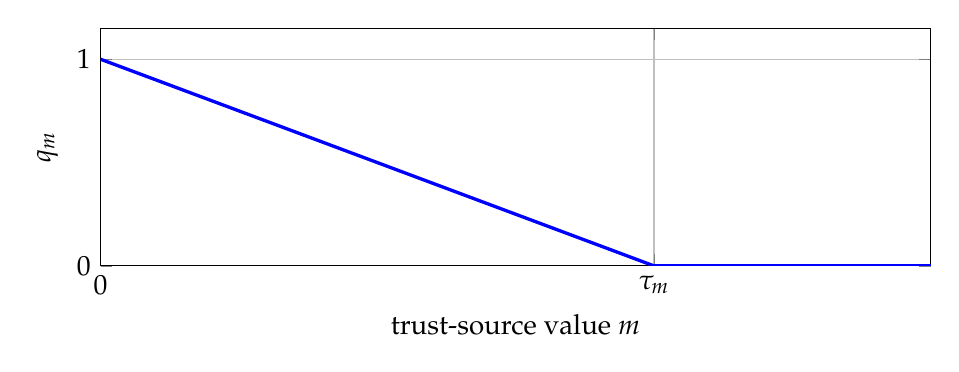
\begin{tikzpicture}
      \begin{axis}[width=\linewidth, height=4.6cm, xmin=0, xmax=1.5, ymin=0, ymax=1.15,
        xlabel={trust-source value $m$}, ylabel={$q_m$}, xtick={0,1}, xticklabels={$0$,$\tau_m$},
        ytick={0,1}, grid=major, every axis plot/.append style={very thick}]
        \addplot[blue] coordinates {(0,1) (1,0) (1.5,0)};
      \end{axis}
    \end{tikzpicture}
    \caption{Lower is better, \cref{eq:dataset-trust:q-low}.}
  \end{subfigure}
  \hfill
  \begin{subfigure}{0.46\textwidth}
    \centering
    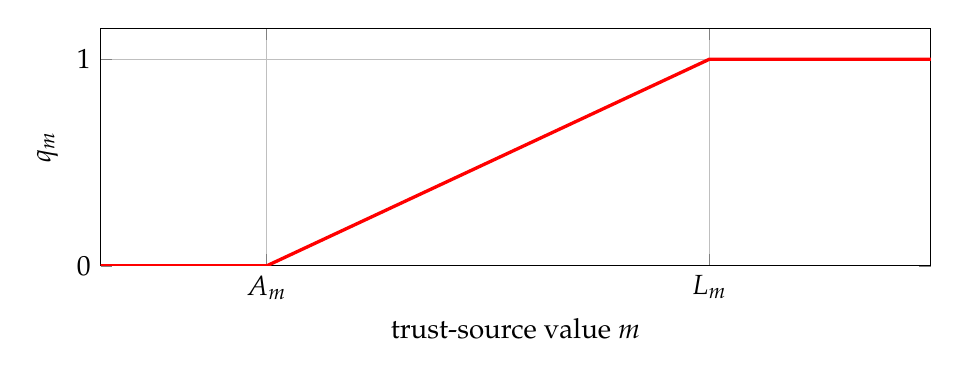
\begin{tikzpicture}
      \begin{axis}[width=\linewidth, height=4.6cm, xmin=0, xmax=1.5, ymin=0, ymax=1.15,
        xlabel={trust-source value $m$}, ylabel={$q_m$}, xtick={0.3,1.1}, xticklabels={$A_m$,$L_m$},
        ytick={0,1}, grid=major, every axis plot/.append style={very thick}]
        \addplot[red] coordinates {(0,0) (0.3,0) (1.1,1) (1.5,1)};
      \end{axis}
    \end{tikzpicture}
    \caption{Higher is better, \cref{eq:dataset-trust:q-high}.}
  \end{subfigure}
  \caption{The two normalization ramps mapping a trust-source value $m$ to a quality score $q_m \in [0,1]$.}
  \label{fig:dataset-trust:ramps}
\end{figure}

The quality score is then converted into positive and negative evidence counts:
\begin{equation}
r_m = K_m \, q_m, \qquad s_m = K_m \, (1 - q_m),
\label{eq:dataset-trust:evidence-counts}
\end{equation}
where $K_m$ is an \emph{evidence-strength} parameter fixing the total amount of evidence the trust source is assumed to provide ($r_m + s_m = K_m$). A large $K_m$ means the analyst takes the trust source seriously; a small $K_m$ means it is weak or only indicative. Under \ac{BPQ} with prior weight $W$ (below), a single trust source contributes residual uncertainty $u = W/(W + K_m)$, so $K_m$ also controls how much uncertainty one trust source leaves.

Trust sources that already produce \emph{counts} (a number of agreeing annotators, a number of contributors above a threshold, a number of classes inside a tolerance zone) skip the ramp: their counts are used directly as $(r, s)$. The \ac{GTSRB} and CIFAR-10H applications are of this kind.

\subsubsection{From evidence to opinions}
\label{sec:dataset-trust:formal:quantification}
The three quantification schemes of \cref{sec:trust_quant_model} map $(r, s)$ to an opinion $(b, d, u)$; we only recall their intuition here and refer to \cref{eq:baseline_quant_meth,eq:weight_quant_meth,eq:constant_quant_meth} for the formulas.
\begin{itemize}
  \item \textbf{\acf{BPQ}}: $u = W/(W + r + s)$, so uncertainty shrinks as evidence accumulates, at a rate set by the prior weight $W$. It is the default when the trust source returns a value with no indication of its own confidence.
  \item \textbf{\acf{EWQ}}: each piece of evidence carries its own weight $w$, so the \emph{quality} of the evidence, not only its amount, drives the uncertainty. It applies when the trust source provides a per-observation confidence (e.g., an annotator's self-reported confidence).
  \item \textbf{\acf{CUQ}}: the uncertainty is fixed externally to a value $U$ (by domain policy or by trust-source metadata) and the remaining mass $1-U$ is split between belief and disbelief in proportion to $r$ and $s$. It applies when the confidence of the assessment is bounded by something other than the number of observations.
\end{itemize}
The analyst picks one scheme per leaf according to the nature of the evidence the trust source produces; the applications exercise BPQ and CUQ, and identify where EWQ would apply (\cref{sec:dataset-trust:applications:gtsrb:method2,sec:dataset-trust:applications:cifar10h}).

\subsubsection{Setting the hyperparameters}
\label{sec:dataset-trust:framework:hyperparameters}
Phase~II introduces four kinds of hyperparameters: the normalization thresholds ($\tau_m$, or $A_m$ and $L_m$), the evidence strength $K_m$, the prior weight $W$, and, under \ac{CUQ}, the fixed uncertainty $U$. Their values are part of the assessment and must be reported with it. We recommend the following.
\begin{itemize}
  \item \textbf{Thresholds.} They encode what the application considers acceptable and are therefore \emph{domain} decisions, not statistical ones. The most principled sources are regulatory or contractual requirements (e.g., a maximum re-identification risk, a minimum coverage of a protected group) and expert elicitation, which is standard practice in risk assessment and is how acceptance criteria are set in safety and conformity assessment. When neither is available, a practical fallback is the empirical distribution of the trust-source value across datasets known to be acceptable, from which $\tau_m$ (or $A_m$, $L_m$) is read as a quantile. Sensitivity analysis, as done for the tolerance $\eta$ in \cref{sec:dataset-trust:applications:gtsrb:eval}, should accompany any threshold choice: a threshold inside a region where the opinion is stable is defensible even if it was elicited.
  \item \textbf{Evidence strength $K_m$.} A uniform value is appropriate when there is no prior reason to weight one trust source over another; this is what we do in the \ac{COMPAS} application. Differing authority (an audited metric versus a heuristic) is expressed by setting $K_m$ proportionally.
  \item \textbf{Prior weight $W$.} $W = 2$ is the non-informative default of \cref{chap:rw}; a larger $W$ (5--10) is preferable for noisy trust sources, since it slows the decrease of uncertainty.
\end{itemize}

\subsection{Phase~III --- Expression Evaluation}
\label{sec:dataset-trust:framework:phase3}
Once the leaf opinions are quantified, the expression assembled in Phase~I is evaluated bottom-up with the \ac{SL} operators: fusion within each stage (\cref{eq:dataset-trust:metric-aggregation}), conjunction across stages (\cref{eq:dataset-trust:lifecycle-decomposition}). The result is an opinion on the original proposition together with the stage-level opinions, which are kept as part of the output because they carry the diagnostic information (which stage is weak, and whether it is weak because of negative evidence or because of missing evidence).

\subsection{Cross-granularity composition of trust sources}
\label{sec:dataset-trust:formal:granularity}

The granularity $\propG$ of the property being assessed and the granularity of the trust sources used to assess it are two related choices. A dataset-level property does not need to be evaluated only by dataset-level trust sources; it can equally be assessed by aggregating evidence collected at finer granularities. Similarly, an entry-level property can rely on feature-level evidence about the columns that compose the entry. Trust sources at a finer granularity than the property can be used, as long as their evidence is aggregated up to the level at which the property is defined. The composition flows upward along the granularity hierarchy:
\[\fGran \to \eGran \to \dGran\]

Two complementary mechanisms support this upward aggregation.
\begin{itemize}
    \item \textbf{Opinion composition.} The property is decomposed unit by unit at the finer granularity. Each unit (feature or entry) is assigned a trust source, which produces an \ac{SL} opinion for that unit. The per-unit opinions are then combined into a coarser-grained opinion using \ac{SL} fusion operators, reflecting the assumption that the units jointly constitute the higher-level object.

    \item \textbf{Evidence lifting.} A single trust source produces per-unit outcomes at the finer granularity. A threshold is applied to each outcome: units that satisfy the property contribute positive evidence, and those that do not contribute negative evidence. The resulting counts are then quantified with one of the three schemes of \cref{sec:dataset-trust:formal:quantification} to produce a single opinion at the coarser level.
\end{itemize}
\noindent An entry is a structured combination of features. Both mechanisms can be applied at any level of the granularity hierarchy, moving evidence upward from features to entries, from entries to the dataset, or directly from features to the dataset. The two can also be chained, for instance by first composing feature-level opinions into per-entry opinions and then lifting those to the dataset level. Because entry- and feature-level trust sources operate on one entry at a time, they apply unchanged to a single input presented at inference time; this is how \cref{chap:patas} obtains input-level opinions.

\subsection{Overview of the Applications}
\label{sec:dataset-trust:framework:applications-overview}
The next three sections instantiate the framework. They cover part of the design space (\cref{tab:dataset-trust:applications-summary}): they were selected to show different properties, different stages and different granularities, and to serve three distinct purposes, which we state up-front because they determine how the results should be read.

\begin{description}
  \item[\ac{COMPAS} (\cref{sec:dataset-trust:applications:compas}) --- an \emph{illustration} of multi-stage composition.]\hfill\\ A tabular dataset for which trust sources exist at all four lifecycle stages. There is no ground truth for ``overall trustworthiness'', so this application does not evaluate the framework; it walks through Phases~I--III end-to-end on a real dataset and shows what the stage-level opinions add over a scalar score. Research question: \emph{can the framework compose heterogeneous stage-level evidence into a dataset-level opinion that remains traceable to the stage that weakened it?}
  \item[\ac{GTSRB} (\cref{sec:dataset-trust:applications:gtsrb}) --- an \emph{evaluation} of two trust sources for one property.]\hfill\\ An image-classification dataset whose class imbalance is known and controllable, so the trust opinion can be compared against a ground truth (the class distribution) and against its downstream effect (the accuracy gap of a trained \ac{CNN}). Research question: \emph{do the trust opinions track a known imbalance and its effect on the model, both when the global distribution is observable (centralized) and when it is not (federated)?}
  \item[CIFAR-10H (\cref{sec:dataset-trust:applications:cifar10h}) --- an \emph{evaluation} at the entry level.]\hfill\\ An image dataset in which every image carries about fifty independent human labels, so per-entry disagreement is directly observable. Research question: \emph{do per-entry opinions derived from annotator agreement identify genuinely ambiguous items, and does their uncertainty respond correctly to the amount of annotation?}
\end{description}
Each application opens with its position in the design space, introduces its dataset, states the trust proposition, and closes with what the example showed. The applications are presented multi-stage first (the general case), then sampling (dataset level), then annotation (entry level).

\FloatBarrier

% ==============================================================
\section{Multi-stage Assessment: COMPAS}
\label{sec:dataset-trust:applications:compas}
\begin{mdframed}[backgroundcolor=blue!4, linewidth=0pt]
\textbf{Position in the design space.}

$\propP$ = overall trustworthiness (conjunction of representativeness, accuracy, fairness, privacy and integrity, \cref{sec:dataset-trust:framework:phase1});\

$\propS = \{\textsc{sampling}, \textsc{collection}, \textsc{annotation},
        \textsc{processing}\}$;\

$\propG$ = dataset;\

\textbf{Quantification:} \ac{BPQ}.

\textbf{Purpose:} illustration of multi-stage composition (original to this dissertation).
\end{mdframed}

This application walks through the three phases of the framework end-to-end on a real dataset. Its purpose is to show how heterogeneous evidence from the four lifecycle stages is composed into one dataset-level opinion while remaining traceable to the stage that produced it; it is not an evaluation against a ground truth, since no reference value of ``overall trustworthiness'' exists for a dataset\footnote{The raw values reported in this section are computed with the implementation developed for this chapter, available at \url{https://github.com/Ouatt-Isma/-Trustworthiness-of-AI-Training-Dataset}. The repository documents the exact computation of every trust source; this section defines them at the level needed to follow the assessment.}.

\paragraph{Dataset.}
\ac{COMPAS} is a commercial recidivism risk-assessment tool used by US courts. The dataset used here is the ``two-year'' file released by ProPublica in its \emph{Machine Bias} investigation~\cite{angwin2016machine}: records of $7{,}214$ defendants screened with \ac{COMPAS} in Broward County, Florida, between 2013 and 2014, joined with public criminal records covering the following two years. After the standard ProPublica filtering (charge date within 30 days of the screening date, valid recidivism record), $6{,}172$ defendants remain. Each record contains demographic attributes (sex, age, age category, race), criminal history (number of prior offenses and juvenile counts), the current charge (degree, description, jail entry and exit dates), the \ac{COMPAS} risk decile (\texttt{decile\_score}, 1--10), direct identifiers (name, date of birth), and the label \texttt{two\_year\_recid} (whether the defendant re-offended within two years; $45.5\%$ positives). The dataset is $51.4\%$ African-American and $34.1\%$ Caucasian, far from the general population. It is a widely studied fairness benchmark: ProPublica showed that the \ac{COMPAS} scores have markedly different false-positive rates across racial groups. It was chosen because it is tabular, with demographic attributes, dates, direct identifiers and an outcome label, so that trust sources of all four lifecycle stages can be computed, and because its construction is publicly documented~\cite{angwin2016machine}.

\paragraph{Trust proposition and expression.}
The proposition is ``the \ac{COMPAS} dataset is trustworthy for training a recidivism classifier''. Phase~I decomposes it along the four stages as in \cref{eq:dataset-trust:lifecycle-decomposition}; at each stage we attach the trust sources of \cref{tab:dataset-trust:catalogue} that can be computed from the available columns, all at dataset granularity. Note that in \ac{COMPAS} the ``annotation'' stage is the recording of the recidivism outcome from court records, not a human labeling campaign: there are no multiple annotators, so the only applicable annotation trust source is the group-label bias index. \cref{tab:dataset-trust:compas-sources} defines the thirteen trust sources retained, as computed on \ac{COMPAS}, together with the threshold used for each.

\begin{table}[!htbp]
  \centering
  \small
  \renewcommand{\arraystretch}{1.15}
  \begin{tabular}{@{}llp{7.9cm}l@{}}
    \toprule
    \textbf{Stage} & \textbf{Source} & \textbf{Definition on COMPAS} & \textbf{Threshold} \\
    \midrule
    \multirow{9}{*}{Sampling}
      & DG   & \ac{KL} divergence between the racial distribution of the dataset and a census-based reference distribution of the general population ($\downarrow$). & $\tau=0.30$ \\
      & MCR  & Ratio of the frequency of African-Americans in the dataset to their frequency in the reference population ($\uparrow$). & $A=0.5$, $L=1$ \\
      & LTCI & Fraction of rare charge descriptions ($<1\%$ of records) that still occur in the most recent half of the records ($\uparrow$). & $A=0.3$, $L=1$ \\
      & DFI  & Mean freshness of records, decaying linearly from 1 at the reference date to 0 one year earlier; the reference date is the latest \texttt{c\_jail\_in} ($\uparrow$). & $A=0$, $L=1$ \\
      & MSA  & Fraction of records missing at least one essential field (race, sex, age, priors, decile score, label) ($\downarrow$). & $\tau=0.10$ \\
    \midrule
    \multirow{9}{*}{Collection}
      & ORR  & Fraction of decile scores outside the valid range $[1,10]$ ($\downarrow$). & $\tau=0.05$ \\
      & MDD  & Largest difference in missingness rate of the essential fields between racial groups ($\downarrow$). & $\tau=0.20$ \\
      & PIID & Fraction of columns that are direct identifiers (name, first, last, dob) ($\downarrow$). & $\tau=0.001$ \\
      & SALS & In-sample accuracy of a logistic regression predicting race from the non-sensitive features (age, priors, juvenile counts, decile score) ($\downarrow$). & $\tau=0.70$ \\
      & RRS  & Mean inverse size of the anonymity set defined by the quasi-identifiers (sex, race, age category), i.e., $k$-anonymity risk ($\downarrow$). & $\tau=0.50$ \\
    \midrule
    Annotation
      & GLBI & \ac{KL} divergence between the label distributions of African-American and Caucasian defendants ($\downarrow$). & $\tau=0.20$ \\
    \midrule
    \multirow{2}{*}{Processing}
      & DIOR & Fraction of exact duplicate rows ($\downarrow$). & $\tau=0.01$ \\
      & FLCA & Maximum absolute Pearson correlation between any numeric feature and the label, a shortcut/leakage indicator ($\downarrow$). & $\tau=0.60$ \\
    \bottomrule
  \end{tabular}
  \caption{Trust sources used in the \ac{COMPAS} assessment. $\downarrow$: lower is better, normalized with \cref{eq:dataset-trust:q-low}; $\uparrow$: higher is better, normalized with \cref{eq:dataset-trust:q-high}. Evidence strength $K_m = 2$ and prior weight $W = 2$ for all trust sources.}
  \label{tab:dataset-trust:compas-sources}
\end{table}

The thresholds were set as follows\footnote{We stress that these values are illustrative. $\tau_{\text{DG}} = 0.30$ tolerates at most $0.30$ nats of divergence from the reference population; $A_{\text{MCR}} = 0.50$ requires the minority group to be represented at least at half its population rate, with parity ($L = 1$) as the ideal; $\tau_{\text{PIID}} = 0.001$ effectively requires that no direct identifier be present. In a deployment they would be elicited from the domain expert or derived from the applicable requirements, as discussed in \cref{sec:dataset-trust:framework:hyperparameters}. Whether this is practical depends on the setting: for regulated domains such as criminal justice or medical devices, acceptance criteria of this kind already have to be documented, so the elicitation cost is incurred anyway; the framework simply makes them explicit inputs of the assessment.}: for each trust source we asked what value a domain expert would consider clearly unacceptable and, for higher-is-better sources, what value would be ideal. All trust sources use the same evidence strength $K_m = 2$ (no prior reason to weight one over another) and the non-informative prior weight $W = 2$.

\subsection{Stage quantification on COMPAS}
\label{sec:dataset-trust:applications:compas:stages}

 \paragraph{Sampling stage.}
The sampling-stage proposition is \emph{``the sampling stage of the \ac{COMPAS} dataset is trustworthy.''} Five trust sources contribute evidence: DG, MCR, LTCI, DFI and MSA. We walk through this stage in detail to illustrate Phase~II; for the sake of brevity, we only summarize the final assessment results of the other three stages (\cref{tab:dataset-trust:compas}).

\subparagraph{Step~1: Normalizing the values.}
The observed values are
\[
\text{DG} = 0.432,\quad \text{MCR} = 3.597,\quad
\text{LTCI} = 0.657,\quad \text{DFI} = 0.100,\quad
\text{MSA} = 0.000.
\]
DG and MCR both compare the dataset to the reference population: the divergence is large (DG $= 0.432 > \tau_{\text{DG}}$), and African-Americans are over-represented by a factor $3.6$ with respect to their population share. DFI is computed with the dataset's own most recent record as the reference ``now''; in practice, freshness should be measured relative to the time at which the dataset is consumed, so the present convention is conservative and for illustration only. Applying \cref{eq:dataset-trust:q-low,eq:dataset-trust:q-high} with the thresholds of \cref{tab:dataset-trust:compas-sources} yields
\[
q_{\text{DG}}   = 0.000,\quad
q_{\text{MCR}}  = 1.000,\quad
q_{\text{LTCI}} = 0.510,\quad
q_{\text{DFI}}  = 0.100,\quad
q_{\text{MSA}}  = 1.000.
\]

\subparagraph{Step~2: Converting to evidence.}
With $K_m = 2$ for every trust source, $r_m = 2 q_m$ and $s_m = 2(1 - q_m)$ give
\[
\begin{aligned}
& r_{\text{DG}}   = 0.00,\ s_{\text{DG}}   = 2.00, \quad
  r_{\text{MCR}}  = 2.00,\ s_{\text{MCR}}  = 0.00, \\
& r_{\text{LTCI}} = 1.02,\ s_{\text{LTCI}} = 0.98, \quad
  r_{\text{DFI}}  = 0.20,\ s_{\text{DFI}}  = 1.80, \\
& r_{\text{MSA}}  = 2.00,\ s_{\text{MSA}}  = 0.00.
\end{aligned}
\]

\subparagraph{Step~3: Applying \ac{BPQ} and fusing.}
\ac{BPQ} with prior weight $W = 2$ gives one opinion per trust source,
\begin{align}
 \omega_{\text{DG}}   &= (0, 0.5, 0.5), \quad&
  \omega_{\text{MCR}}  &= (0.5, 0, 0.5),\\
\omega_{\text{LTCI}} &= (0.255, 0.245, 0.5), \quad&
  \omega_{\text{DFI}}  &= (0.05, 0.45, 0.5), \\
\omega_{\text{MSA}}  &= (0.5, 0, 0.5),
\end{align}
and cumulative fusion of the five opinions (\cref{eq:dataset-trust:metric-aggregation}) gives the stage-level opinion
\[
\omega_{\text{sampling}} = (0.435,\ 0.398,\ 0.167).
\]
Under \ac{BPQ}, cumulative fusion amounts to adding the evidence counts, so the stage opinion is simply $\bigl(\sum r_m,\ \sum s_m\bigr) = (5.22,\ 4.78)$ quantified with $W = 2$; this makes the stage-level result easy to audit.

\subparagraph{Interpretation.}
The opinion $(0.435,\ 0.398,\ 0.167)$ has belief and disbelief close to each other and a comparatively low uncertainty: the evidence base is large enough for the opinion to be decisive, but the evidence itself is genuinely mixed. Two trust sources contribute positive evidence: the minority coverage rate ($q_{\text{MCR}} = 1.00$) and the missing-at-source audit ($q_{\text{MSA}} = 1.00$). Two contribute negative evidence: the distribution gap ($q_{\text{DG}} = 0.00$) and the data freshness index ($q_{\text{DFI}} = 0.10$). The long-tail coverage index ($q_{\text{LTCI}} = 0.51$) is mixed. Rather than collapsing these into a single ``the sampling is good'' or ``the sampling is bad'' verdict, the framework reports both: the dataset has acceptable minority coverage and structural completeness, but exhibits a distribution gap with respect to the reference population and is stale. The two signals are surfaced separately rather than averaged away.

\begin{table}[!htbp]
  \centering
  \small
  \renewcommand{\arraystretch}{1.1}
  \begin{tabular}{@{}llrrl@{}}
    \toprule
    \textbf{Stage} & \textbf{Trust source} & \textbf{Raw} & \textbf{$q$} & \textbf{Direction / Threshold} \\
    \midrule
    \multirow{5}{*}{Sampling}
      & DG                                  & 0.432  & 0.000 & lower is better \{$\tau{=}0.3$\} \\
      & MCR(African-American)           & 3.597 & 1.000 & higher is better \{$A{=}0.5$, $L{=}1.0$\} \\
      & LTCI(c\_charge\_desc)               & 0.657  & 0.510 & higher is better \{$A{=}0.3$, $L{=}1.0$\}\\
      & DFI(c\_jail\_in)                    & 0.100 & 0.100 & higher is better \{$A{=}0$, $L{=}1.0$\} \\
      & MSA(essential\_cols)                & 0.000  & 1.000 & lower is better \{$\tau{=}0.1$\} \\
    \cmidrule(lr){2-5}
      & \multicolumn{4}{l}{\ac{BPQ} stage opinion: $(b, d, u) = (0.435,\ 0.398,\ 0.167)$\quad \{$W{=}2$\}} \\
    \midrule
    \multirow{5}{*}{Collection}
      & ORR(decile\_score)                  & 0.000  & 1.000 & lower is better \{$\tau{=}0.05$\} \\
      & MDD(by\_race)                       & 0.000  & 1.000 & lower is better \{$\tau{=}0.2$\} \\
      & PIID                                & 0.075  & 0.000 & lower is better \{$\tau{=}0.001$\} \\
      & SALS(race$\,|\,$features)           & 0.570  & 0.186 & lower is better \{$\tau{=}0.7$\} \\
      & RRS(qid$=$sex,race,age\_cat)        & 0.191  & 0.619 & lower is better \{$\tau{=}0.5$\} \\
    \cmidrule(lr){2-5}
      & \multicolumn{4}{l}{\ac{BPQ} stage opinion: $(b, d, u) = (0.467,\ 0.366,\ 0.167)$\quad \{$W{=}2$\}} \\
    \midrule
    Annotation
      & GLBI(two\_year\_recid$\,|\,$race)   & 0.036  & 0.821 & lower is better \{$\tau{=}0.2$\} \\
    \cmidrule(lr){2-5}
      & \multicolumn{4}{l}{\ac{BPQ} stage opinion: $(b, d, u) = (0.411,\ 0.089,\ 0.500)$\quad \{$W{=}2$\}} \\
    \midrule
    \multirow{2}{*}{Processing}
      & DIOR                                & 0.000  & 1.000 & lower is better \{$\tau{=}0.01$\}  \\
      & FLCA                                 & 0.291   & 0.516 & lower is better \{$\tau{=}0.6$\}  \\
    \cmidrule(lr){2-5}
      & \multicolumn{4}{l}{\ac{BPQ} stage opinion: $(b, d, u) = (0.505,\ 0.161,\ 0.333)$\quad \{$W{=}2$\}} \\
    \bottomrule
  \end{tabular}
  \caption{Raw values, quality scores and stage-level opinions for \ac{COMPAS} ($K_m = 2$ for every trust source). Each stage is quantified independently with \cref{eq:dataset-trust:q-low,eq:dataset-trust:q-high} and \ac{BPQ}; the dataset-level opinion is obtained by the cross-stage conjunction of \cref{eq:dataset-trust:lifecycle-decomposition}.}
  \label{tab:dataset-trust:compas}
\end{table}

\paragraph{Collection stage.}
The collection stage produces a more balanced assessment, with belief $b = 0.467$, disbelief $d = 0.366$ and uncertainty $u = 0.167$. The measurement-integrity trust sources, out-of-range rate ($q = 1.000$) and missing-data disparity ($q = 1.000$), contribute positive evidence: the decile scores are all in range and missingness does not differ across racial groups. The privacy trust sources, however, contribute substantial negative evidence: the file ships with direct identifiers (\ac{PII} density $q = 0.00$), race can be predicted from the non-sensitive features with $57\%$ accuracy (sensitive-attribute leakage $q = 0.186$), and the quasi-identifiers leave a non-negligible re-identification risk ($q = 0.619$). Privacy is part of the property being assessed (overall trustworthiness, as defined in \cref{sec:dataset-trust:framework:phase1}, includes privacy compliance), so this evidence legitimately lowers the collection-stage opinion; an analyst assessing a narrower property such as measurement accuracy would prune the privacy trust sources and obtain a clearly positive collection-stage opinion. The resulting opinion reflects a trade-off between accurate measurement and privacy exposure rather than a clear conclusion.

\paragraph{Annotation stage.}
The annotation stage is assessed with a single trust source, the group-label bias index, whose value ($0.036$ nats) is well within tolerance and gives $q = 0.821$. The stage-level opinion is $(b, d, u) = (0.411, 0.089, 0.500)$: the lowest belief of the four stages. This low belief should not be read as ``the annotation is not trustworthy'': disbelief is correspondingly low, and the dominant mass is uncertainty. The framework is reporting that, with only one trust source available ($r + s = K_m = 2$), it does not have enough evidence to be confident in either direction. This is qualitatively different from the sampling-stage opinion, which has comparable belief but reached it through balanced positive and negative evidence rather than through absent evidence.

\paragraph{Processing stage.}
The processing stage yields the strongest signal, with belief $b = 0.505$, disbelief $d = 0.161$ and uncertainty $u = 0.333$. The absence of duplicate rows provides strong positive evidence ($q = 1.00$), and the feature--label correlation audit ($q = 0.516$, maximum correlation $0.29$ with \texttt{priors\_count}) is mildly positive. Residual uncertainty remains because only two processing-stage diagnostics can be computed on a dataset whose cleaning history is not available.

\paragraph{Cross-stage rollup.}
The four stage-level opinions are combined into a dataset-level trustworthiness opinion by the cross-stage conjunction of \cref{eq:dataset-trust:lifecycle-decomposition}:
\[
\omega_{\dataset}
= \omega_{\text{sampling}} \cdot
  \omega_{\text{collection}} \cdot
  \omega_{\text{annotation}} \cdot
  \omega_{\text{processing}} = (0.12,\ 0.71,\ 0.17).
\]
The result is dominated by disbelief: the evidence accumulated across the four stages points against the trustworthiness of the dataset rather than for it. This is a direct consequence of conjunction: a single stage with high disbelief is sufficient to pull the combined opinion toward disbelief, regardless of how well the other stages perform. Here the collection and sampling stages, both carrying substantial disbelief, are the primary drivers. The residual uncertainty $u = 0.17$ mainly reflects the limited diagnostic coverage of the annotation stage.

\paragraph{What this example showed.}
Read together with \cref{tab:dataset-trust:compas}, the rollup preserves three pieces of information that a scalar quality score would collapse: \emph{which} stage carries the strongest negative signal (collection, through privacy exposure), \emph{which} stage merely lacks evidence (annotation, with $u = 0.50$ from a single trust source), and how the stages compare quantitatively. These correspond to two qualitatively different actions for an auditor: collecting more representative or privacy-aware data attacks the sampling- and collection-stage disbelief, whereas gathering additional annotation-stage diagnostics reduces the annotation-stage uncertainty. The example also showed the two properties of the quantification that make the result auditable: under \ac{BPQ}, fusion within a stage is a sum of evidence counts, and every hyperparameter ($\tau$, $A$, $L$, $K_m$, $W$) is an explicit, reportable input. Finally, it showed the cost of the approach: thirteen threshold values had to be set, and the assessment is only as meaningful as those choices, which is why they are reported alongside the opinions.

\FloatBarrier

% ==============================================================
\section{Sampling Stage, Dataset Level: Representativeness on \acs{GTSRB}}
\label{sec:dataset-trust:applications:gtsrb}

\begin{mdframed}[backgroundcolor=blue!4, linewidth=0pt]
\textbf{Position in the design space.}

$\propP$ = representativeness (class balance);\quad
$\propS = \{\textsc{sampling}\}$;\quad $\propG$ = dataset;\

\textbf{Quantification:} \ac{CUQ} (global-distribution trust source), \ac{BPQ} (local-entropy trust source).\quad

\textbf{Purpose:} evaluation.\quad \textbf{Published in:}~\cite{10.1007/978-3-032-19096-3_17}.
\end{mdframed}

\paragraph{Purpose and research question.}
This application evaluates the framework on one well-defined cell of the design space: the representativeness of the sampling stage, understood as class balance, at dataset granularity. Class balance was chosen because it is a property for which a \emph{ground truth} exists (the class distribution is directly observable and can be manipulated) and whose downstream effect is measurable (the accuracy of a classifier on under-represented classes). The research question is: \emph{do the trust opinions produced by the framework track a known class imbalance and its effect on the trained model, both when the global class distribution is observable (centralized setting) and when it is not (federated setting)?} The federated setting is motivated by the \ac{CCAM} use case of this thesis, in which several \acp{OEM} contribute driving data to a shared training set without disclosing their raw data. It leads to two different trust sources for the same proposition, which in turn exercise two of the three quantification schemes.

\paragraph{Dataset.}
The \acf{GTSRB}~\cite{stallkamp2012man,GTSRB} contains $51{,}839$ color images of German road signs in $K = 43$ classes, split into $39{,}209$ training and $12{,}630$ test images; we resize all images to $32 \times 32$ pixels. The class distribution is documented and strongly non-uniform: the training set holds between $210$ and $2{,}250$ images per class (\cref{fig:gtsrb:distscenario1}(a)). This is not an artifact of the collection: the images were extracted from real drives, so the class frequencies reflect how often each sign occurs on the road. In particular, the fourteen triangular \emph{warning signs} (classes 18--31: dangerous curve, slippery road, pedestrians, children crossing, \dots) are among the rarest classes. Whether such an imbalance is a defect depends on the property assessed: it is acceptable, even desirable, for a proposition about representativeness of deployment-time frequencies, but for the proposition assessed here, class balance with respect to a uniform target, it is precisely what the trust opinion must detect. The documented class distribution is therefore the ground truth against which the opinions are checked, and the warning-sign group is the natural minority group on which to measure the downstream effect; the summary returns to the deployment-frequency reading.

\paragraph{Trust proposition.}
\emph{``The dataset $\dataset$ is not biased with respect to class balance.''} We treat this as a simple trust proposition at dataset level: the expression tree is a single leaf, and the application is entirely about how that leaf is quantified from two different trust sources.

To assess balance, we describe the dataset by its \emph{class-probabilities distribution}. For a classification task with $K$ classes and $N$ data points, the empirical probability of class $k$ is
\begin{equation}
P(\mathrm{Class}_k) = \frac{N_k}{N}, \qquad
\sum_{k=1}^{K} P(\mathrm{Class}_k) = 1,
\end{equation}
where $N_k$ is the number of data points belonging to class $k$. This distribution is the basic object on which both trust sources operate. A perfectly balanced dataset has all probabilities equal to $1/K$; the density of the class-probability distribution is then concentrated around $1/K$. Imbalanced datasets exhibit a wider spread. \Cref{fig:gtsrb:probability-density} illustrates this on a \emph{synthetic toy configuration}, unrelated to \ac{GTSRB}, with $K = 6$ classes and $N = 5200$ points: an imbalanced dataset with class counts $[100,\allowbreak 100,\allowbreak 1000,\allowbreak 1000,\allowbreak 1000,\allowbreak 2000]$ and a balanced one with class counts $[857,\allowbreak 857,\allowbreak 867,\allowbreak 867,\allowbreak 876,\allowbreak 876]$.

\begin{figure}[!htbp]
    \centering
    \begin{subfigure}{0.45\textwidth}
        \centering
        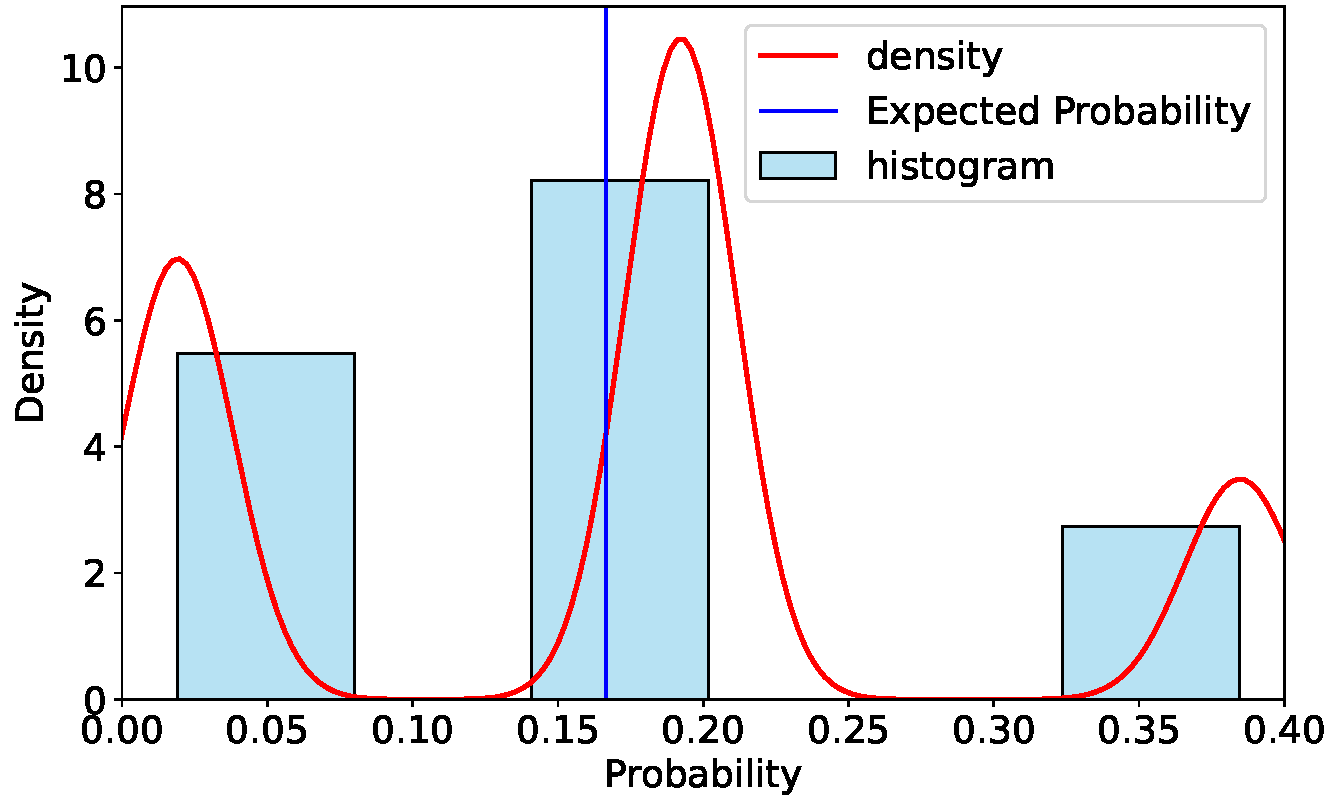
\includegraphics[width=0.95\linewidth]{img/data/imbalanced.pdf}
        \caption{Imbalanced dataset.}
    \end{subfigure}
    \begin{subfigure}{0.45\textwidth}
        \centering
        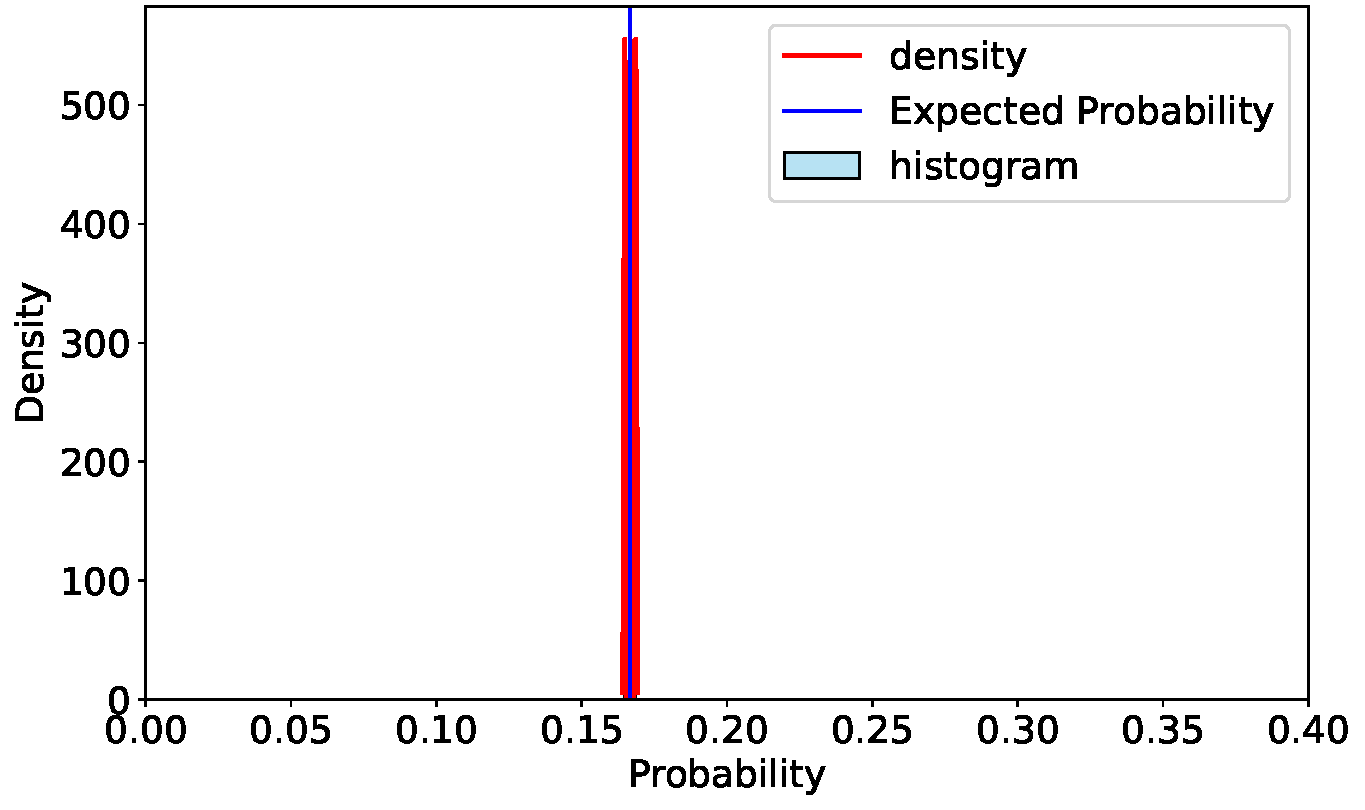
\includegraphics[width=0.95\linewidth]{img/data/balanced.pdf}
        \caption{Balanced dataset.}
    \end{subfigure}
    \caption{Density of the class-probabilities distribution for a synthetic toy example ($N = 5200$ points, $K = 6$ classes; not \ac{GTSRB}). The balanced dataset concentrates around $1/K \approx 0.167$; the imbalanced dataset shows a wider spread.}
    \label{fig:gtsrb:probability-density}
\end{figure}

\subsection{Global-distribution trust source (GD)}
\label{sec:dataset-trust:applications:gtsrb:method1}

The first trust source, which we call the \emph{global-distribution} (GD) trust source, operates on the global class-probabilities distribution directly. A class is considered \emph{balanced} when its empirical probability lies within a tolerance interval around the expected value:
\begin{equation}
P(\mathrm{Class}_k) \in
  \left[\frac{1}{K} - \eta_1,\ \frac{1}{K} + \eta_2\right].
\label{eq:gtsrb:tolerance-zone}
\end{equation}
The parameters $\eta_1, \eta_2$ control the width of the tolerance zone and play the same role as the threshold $\tau_m$ in \cref{eq:dataset-trust:q-low}: they define the boundary beyond which a class probability is considered unacceptably imbalanced. We set $\eta = \eta_1 = \eta_2$ for the experiments reported below; the impact of $\eta$ is studied in \cref{sec:dataset-trust:applications:gtsrb:eval}.

Each class provides one piece of evidence: positive if its probability falls inside the tolerance zone, negative otherwise. Normalized by $K$, positive evidence is the area under the density $f$ of the class-probabilities distribution that falls within the tolerance zone, and negative evidence the complementary area:
\begin{equation}
r = \int_{1/K - \eta_1}^{1/K + \eta_2} f(x)\, dx
  = \frac{n_t}{K},
\qquad
s = 1 - r,
\label{eq:gtsrb:method1-evidence}
\end{equation}
where $n_t$ is the number of classes whose empirical probability falls within the tolerance zone.

\paragraph{Quantification scheme: \ac{CUQ}.}
The GD evidence is naturally normalized ($r + s = 1$), so the remaining choice is how to set the uncertainty mass. The GD trust source measures balance from the empirical class-probabilities distribution, which is itself estimated from the dataset: a \emph{small} dataset gives a noisy estimate, so the trust opinion should be held with low confidence regardless of how balanced the observed distribution appears. The right notion of \emph{small} is relative to the model's data requirements, which is what \emph{sample complexity} measures in \ac{PAC} learning.

\ac{PAC} learning~\cite{valiant1984theory} asks how many training examples are needed for a learner to find, with probability at least $1 - \delta$, a hypothesis whose error is at most $\epsilon$. For a hypothesis class of \ac{VC} dimension $d$, Haussler et al.~\cite{HAUSSLER1994248} show that the required number of examples is
$\mathcal{M}(\epsilon, \delta) = \mathcal{O}\!\left(\frac{d}{\epsilon}\log\frac{1}{\delta}\right)$.
We use the leading term as a \emph{theoretical} sample complexity,
$N_s = \frac{d}{\epsilon}\log(1/\delta)$,
and set the \ac{CUQ} uncertainty from the gap between $N_s$ and the actual dataset size $N$:
\begin{equation}
U = \min\!\left(
      \max\!\left(
        \frac{\log_{10}(N_s) - \log_{10}(N)}{10},\ m_1\right),\ m_2\right),
\label{eq:gtsrb:uncertainty}
\end{equation}
where $[m_1, m_2]$ is the admissible range of uncertainty (set to $[0,1]$ in our experiments). The division by $10$ maps a gap of ten orders of magnitude to full uncertainty. \Cref{fig:gtsrb:u-vs-n} plots $U$ as a function of $N / N_s$: when $N$ is large relative to $N_s$, the dataset is sufficient for the model and the uncertainty shrinks toward zero; when $N$ is small relative to $N_s$, the assessment cannot be made with confidence regardless of how balanced the observed distribution is. Because of the logarithm, $U$ changes slowly with $N$: multiplying $N$ by ten lowers $U$ by only $0.1$.

The \ac{VC} dimension of a \ac{CNN} is not computable exactly. Following the classical bound for piecewise-linear networks, which grows with the number of parameters $P$ and layers $L$, we use the proxy $d = P \cdot L$. For the \ac{CNN} of \cref{sec:dataset-trust:applications:gtsrb:eval} ($P \approx 1.46 \times 10^{6}$, $L = 17$), $d \approx 2.5 \times 10^{7}$; with $\epsilon = 0.05$ and $\delta = 0.5$ this gives $N_s \approx 3.4 \times 10^{8}$, four orders of magnitude above the $39{,}209$ images of \ac{GTSRB}, hence $U \approx 0.39$ in all centralized experiments. This value is admittedly conservative (\ac{PAC} bounds are worst-case), which is acceptable here since $U$ is used as a \emph{relative} confidence scale across datasets of different sizes rather than as an absolute statement.

\begin{figure}[!htbp]
  \centering
  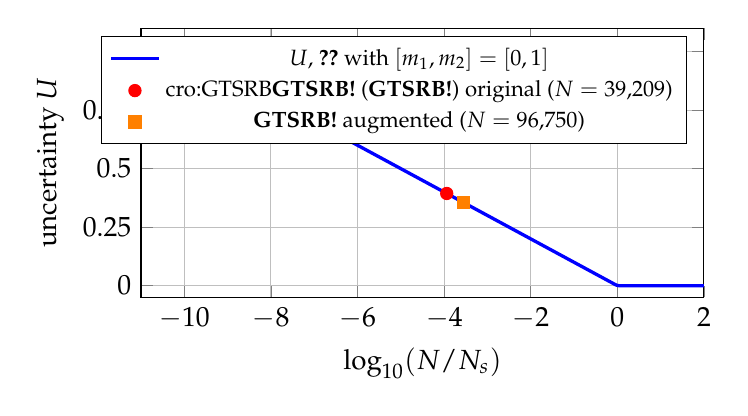
\begin{tikzpicture}
    \begin{axis}[width=0.72\linewidth, height=5cm, xmin=-11, xmax=2, ymin=-0.05, ymax=1.1,
      xlabel={$\log_{10}(N / N_s)$}, ylabel={uncertainty $U$}, grid=major,
      xtick={-10,-8,-6,-4,-2,0,2}, ytick={0,0.25,0.5,0.75,1}, legend pos=north east, legend style={font=\footnotesize}]
      \addplot[very thick, blue, domain=-11:2, samples=200] {min(max(-x/10,0),1)};
      \addlegendentry{$U$, \cref{eq:gtsrb:uncertainty} with $[m_1,m_2]=[0,1]$}
      \addplot[only marks, mark=*, mark size=2.2pt, red] coordinates {(-3.94,0.394)};
      \addlegendentry{\ac{GTSRB} original ($N = 39{,}209$)}
      \addplot[only marks, mark=square*, mark size=2.2pt, orange] coordinates {(-3.55,0.355)};
      \addlegendentry{\ac{GTSRB} augmented ($N = 96{,}750$)}
    \end{axis}
  \end{tikzpicture}
  \caption{\ac{CUQ} uncertainty of the GD trust source as a function of the ratio between the dataset size $N$ and the theoretical sample complexity $N_s$. The two markers are the datasets of Scenario~1 ($N_s \approx 3.4 \times 10^{8}$).}
  \label{fig:gtsrb:u-vs-n}
\end{figure}

Once $U$ is fixed by \cref{eq:gtsrb:uncertainty}, belief and disbelief follow from the \ac{CUQ} formula ($\gamma = (1-U)/(r+s)$, $b = \gamma r$, $d = \gamma s$).

\subsection{Local-entropy trust source (LE)}
\label{sec:dataset-trust:applications:gtsrb:method2}
In federated or collaborative settings, no single party observes the global distribution of class probabilities: each contributing node (e.g., each \ac{OEM} in a vehicular collaborative dataset) only sees its own sub-dataset. The GD trust source can still be applied if every contributor shares its class counts with an aggregator, but in privacy-sensitive settings even class counts may be considered disclosive (they reveal what a contributor's fleet has encountered). The \emph{local-entropy} (LE) trust source takes another path: each node summarizes its sub-dataset with a single scalar, and the aggregator receives only that scalar.

\paragraph{Entropy as a balance proxy.}
Each contributor $i$ computes the entropy of its local
class-probabilities distribution $P^{(i)}$:
\begin{equation}
\mathcal{H}(P^{(i)})
= -\sum_{k=1}^{K} p^{(i)}_k \log p^{(i)}_k.
\end{equation}
Entropy is maximal ($\log K$) when the local distribution is uniform and decreases as one or a few classes dominate.

Each local entropy is compared against a threshold that defines the \emph{edge of acceptable balance}. We construct an \emph{edge-acceptable} distribution $P_E$ by setting each class probability to $1/K \pm \eta$, alternating the sign so that $P_E$ sums to one (with one class set to exactly $1/K$ when $K$ is odd), and define
\begin{equation}
\mathit{Thres} = \mathcal{H}(P_E).
\end{equation}
$P_E$ is the least balanced distribution that the GD trust source would still accept for every class, so $\mathit{Thres}$ is the entropy below which a contributor is, by the same standard, imbalanced. Each contributor then provides exactly one piece of evidence: contributors whose local entropy exceeds $\mathit{Thres}$ provide one unit of positive evidence, the others one unit of negative evidence. Over $M$ contributors,
\begin{equation}
r = \bigl|\{\, i : \mathcal{H}(P^{(i)}) > \mathit{Thres} \,\}\bigr|, \qquad s = M - r.
\label{eq:gtsrb:method2-evidence}
\end{equation}

\paragraph{Why negative evidence rather than exclusion.}
One may ask why an imbalanced contributor is counted as negative evidence instead of simply being removed from the collaborative dataset. The answer is the role of the framework: it \emph{assesses} the dataset as it is, it does not curate it. Whether to drop a contributor is a decision to be taken downstream, on the basis of the opinion; and in the federated setting the aggregator holds no data to drop, only summaries. Moreover, an imbalanced contributor is genuine evidence that the collaborative dataset, as assembled, is at risk of imbalance, which is exactly what the proposition asks.

\paragraph{Quantification scheme: \ac{BPQ}.}
Each contributor produces one binary piece of evidence, so the natural quantification is \ac{BPQ}: as $M$ grows, the residual uncertainty $u = W / (W + M)$ shrinks. This is the desired behavior in a federated setting, where adding more contributors should progressively reduce the uncertainty of the global assessment without requiring any party to disclose its local class distribution.

\paragraph{Blind spot and counter-measure.}
Because each contributor is judged in isolation, the LE trust source cannot see that two locally imbalanced sub-datasets may be \emph{complementary} (one lacking warning signs, the other lacking speed limits) and combine into a globally balanced dataset; both would report negative evidence, pulling the opinion toward disbelief although the union is acceptable. The GD trust source, which sees the global distribution, is immune to this artifact. Two counter-measures are possible within the same privacy budget. The first is to have each contributor additionally report the \emph{identity} of its under-represented classes (a set of class indices, still no counts): the aggregator can then detect complementarity and neutralize the corresponding negative evidence. The second is to compute the global class counts by \emph{secure aggregation}, so that the aggregator learns only the sum of the local counts, which is all the GD trust source needs; this removes the artifact entirely at the cost of a cryptographic protocol. We leave the evaluation of both to future work.

\paragraph{A weighted extension.}
A natural refinement treats the distance $|\mathcal{H}(P^{(i)}) - \mathit{Thres}|$ as an evidence weight, which moves the scheme from \ac{BPQ} to \ac{EWQ}: contributors far from the threshold provide high-weight evidence, contributors near it low-weight evidence. We did not evaluate this extension, for two reasons. First, it introduces one more hyperparameter (the mapping from entropy distance to weight) that would have to be calibrated for each $K$. Second, in the experiments below every contributor is either a near-uniform random share of the same distribution or a share stripped of its warning signs, so the entropy distances are almost bimodal and the weighted variant would behave like the binary one; the setting where it matters, contributors with graded degrees of imbalance, is left to future work.

\subsection{Experimental evaluation}
\label{sec:dataset-trust:applications:gtsrb:eval}

We evaluate both trust sources on the \ac{GTSRB} training set ($N = 39{,}209$, $K = 43$). The downstream model is a \ac{CNN} with three convolutional blocks (64/128/256 filters, $3 \times 3$ kernels), each followed by batch normalization, $2 \times 2$ max-pooling and dropout (rate $0.25$); two fully connected layers (256 and 128 ReLU units); a final dropout of rate $0.5$; and a softmax output of size 43 ($P \approx 1.46 \times 10^{6}$ parameters, $L = 17$ layers). Training uses Adam, sparse categorical cross-entropy, batch size 36 and 5 epochs, on an 80/20 split of the training set; accuracies are reported on the official test set, overall and separately for the warning-sign group (classes 18--31) and the other signs. The expected class probability is $1/K \approx 0.02326$ and the tolerance is fixed at $\eta = 0.02$ for both trust sources (this choice is justified at the end of the section).

We define two scenarios:
\begin{itemize}
  \item \textbf{Scenario 1 (centralized).} A single dataset is assessed, in two variants: the original \ac{GTSRB} training set, and an augmented version in which the minority classes are oversampled with SMOTE~\cite{DBLP:journals/corr/abs-1106-1813}. SMOTE creates a synthetic instance by linear interpolation between a minority-class instance and one of its nearest neighbors of the same class; we apply it to the flattened $32 \times 32 \times 3$ pixel vectors, so a synthetic image is a pixel-wise blend of two real images of the same sign. Every class is oversampled up to the majority count of $2{,}250$, which raises the dataset size from $39{,}209$ to $96{,}750$ images. (Blended images are of limited realism; SMOTE is used here only as a simple way to obtain a perfectly balanced variant of the same dataset.) The GD trust source is the natural choice in this setting since the global class distribution is fully observable; the LE trust source would reduce to a single contributor and add nothing.
  \item \textbf{Scenario 2 (collaborative).} The training set is partitioned \emph{round-robin} across $M$ contributors (image $j$ goes to contributor $j \bmod M$), so that every sub-dataset is a near-uniform random share of the same distribution. A configurable number of contributors is then made \emph{imbalanced} by removing their warning-sign images (classes 18--31), keeping at most one image per warning-sign class so that no class disappears entirely. We sweep the number of imbalanced contributors from $0$ to $M$ and, for each value, assess the collaborative dataset with both trust sources and train the \ac{CNN} on its union. The GD trust source is applied at an aggregator that receives the class counts of every contributor; the LE trust source is applied to the per-contributor entropies only.
\end{itemize}

\paragraph{Scenario~1: original vs.\ augmented dataset.}
\Cref{fig:gtsrb:distscenario1} compares the class distribution and the class-probabilities distribution of the original and augmented datasets. SMOTE flattens the class distribution and concentrates the probability density at $1/K$. The downstream effect is modest in aggregate accuracy ($95.17\%$ vs.\ $95.10\%$) but visible in the per-group accuracy gap, which drops from $5.24$ to $3.88$ percentage points (\cref{tab:gtsrb:acc1}).

The GD trust opinions reflect the same pattern and make it quantitative: the original dataset is assessed as $(b, d, u) = (0.50,\ 0.11,\ 0.39)$ and the augmented dataset as $(0.64,\ 0.00,\ 0.36)$. Three things are worth reading in these numbers. First, the belief and disbelief of the original dataset are consistent with the ground truth: with $\eta = 0.02$, $35$ of the $43$ classes fall inside the tolerance zone and $8$ outside, so the dataset is judged \emph{mostly} balanced with a clear minority of problematic classes, which is what \cref{fig:gtsrb:distscenario1}(a) shows. Second, after augmentation disbelief drops to exactly zero, since every class now has probability $1/K$; this is the correct answer for a perfectly balanced dataset, and belief rises to $1 - U = 0.64$. Third, uncertainty barely moves ($0.39 \to 0.36$) although the dataset has grown by a factor $2.5$: this is the logarithm in \cref{eq:gtsrb:uncertainty} at work ($\log_{10} 2.47 / 10 \approx 0.04$), and it is intended. Relative to the $N_s \approx 3.4 \times 10^{8}$ examples the \ac{PAC} bound asks for, $96{,}750$ images are not meaningfully more than $39{,}209$; the augmented dataset is better \emph{balanced}, but it is not a substantially larger \emph{evidence base} about the model's data needs, and synthetic blends add no new information about the world. The opinion therefore says: ``balanced, but still assessed with limited confidence'', which is the appropriate reading of a SMOTE-augmented dataset.

\begin{figure}[!htbp]
    \centering
    \begin{subfigure}{0.35\textwidth}
        \centering
        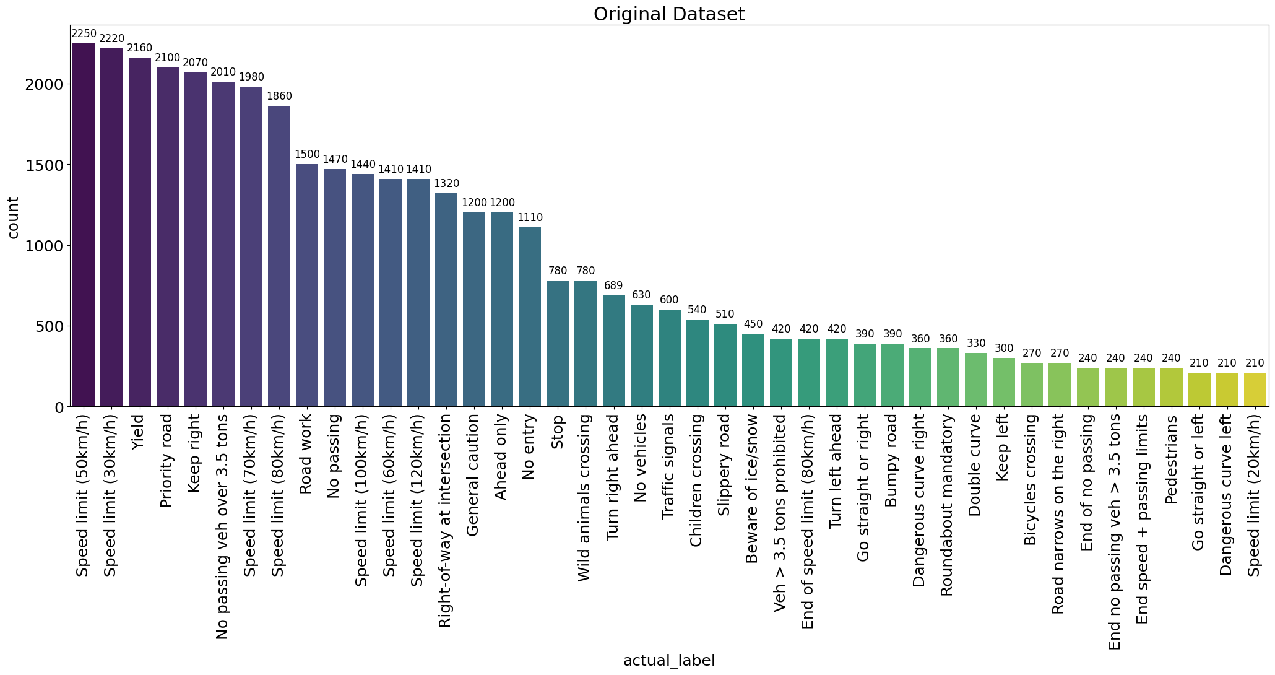
\includegraphics[width=0.95\linewidth]{img/data/evalDist/or.pdf}
        \caption{Class distribution, original.}
    \end{subfigure}
    \begin{subfigure}{0.35\textwidth}
        \centering
        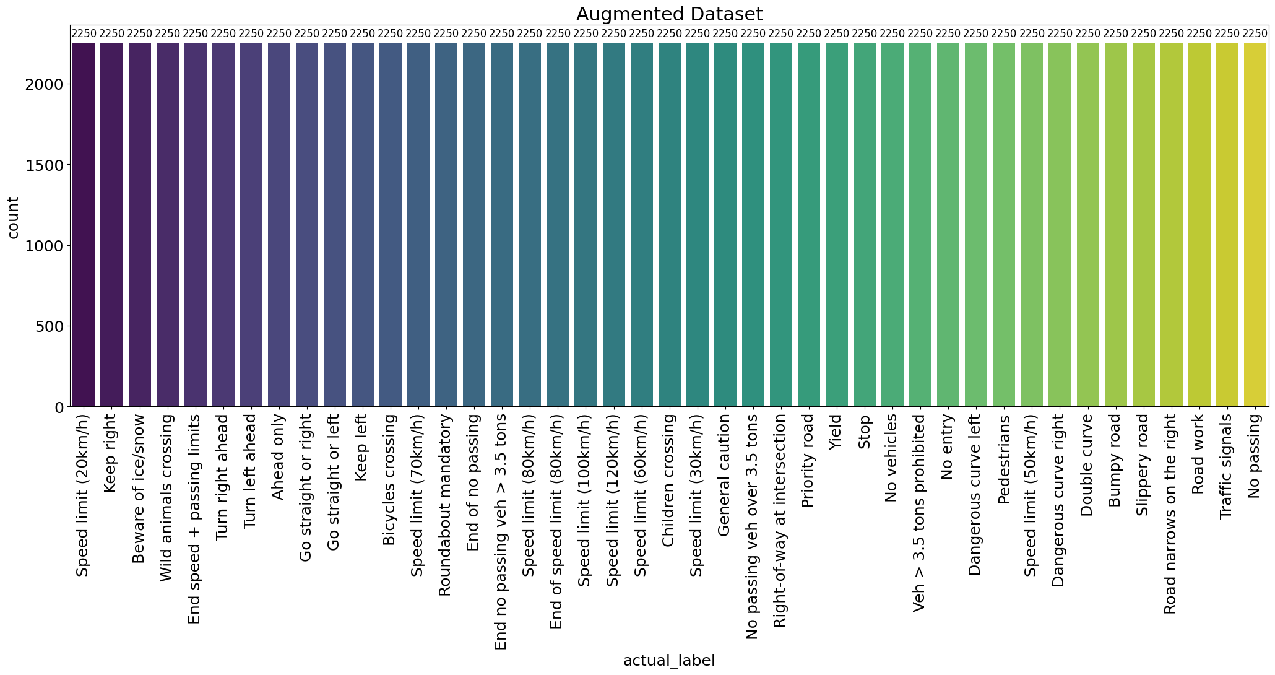
\includegraphics[width=0.95\linewidth]{img/data/evalDist/aug.pdf}
        \caption{Class distribution, augmented.}
    \end{subfigure}
    \begin{subfigure}{0.35\textwidth}
        \centering
        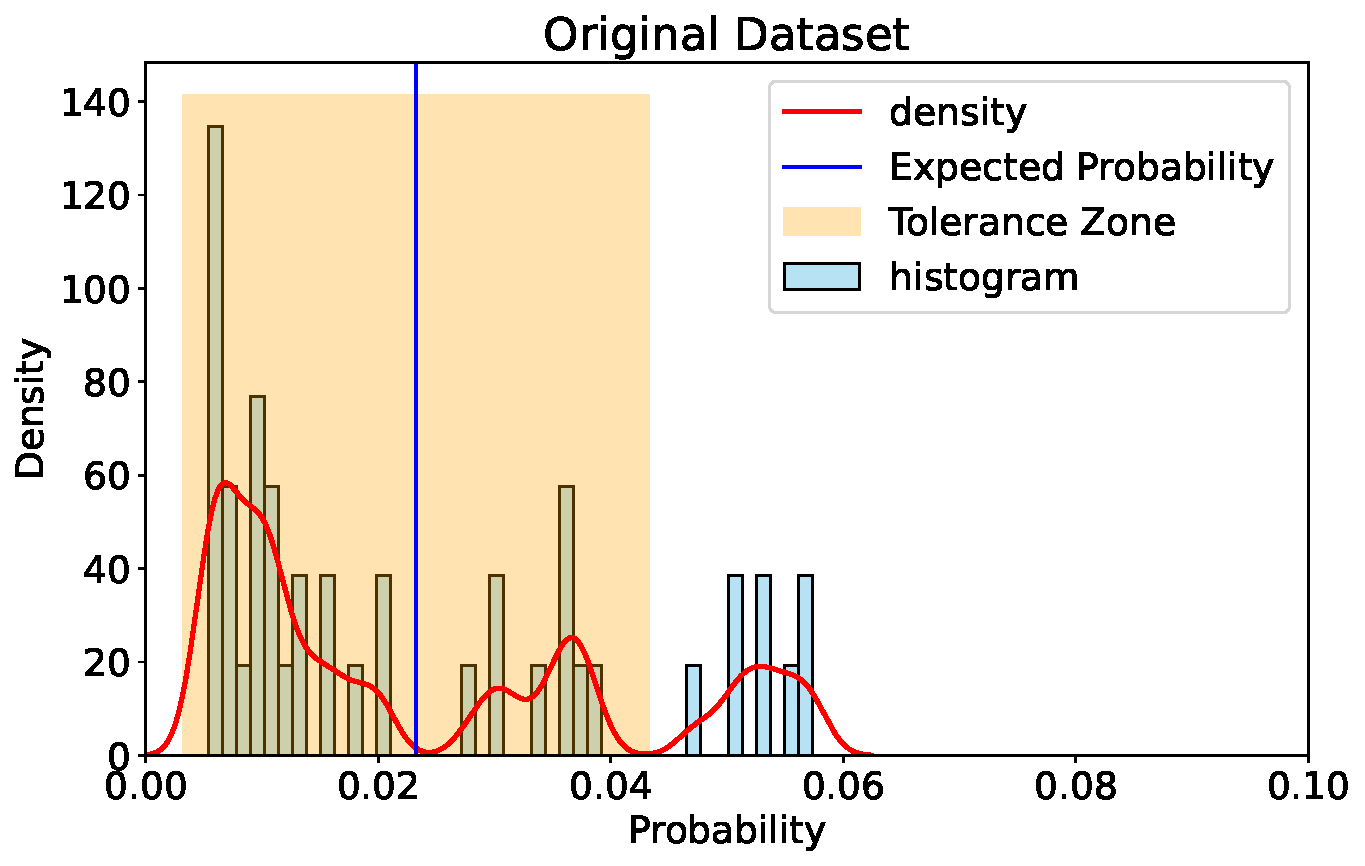
\includegraphics[width=0.95\linewidth]{img/data/evalDist/orp.pdf}
        \caption{Probability distribution, original.}
    \end{subfigure}
    \begin{subfigure}{0.35\textwidth}
        \centering
        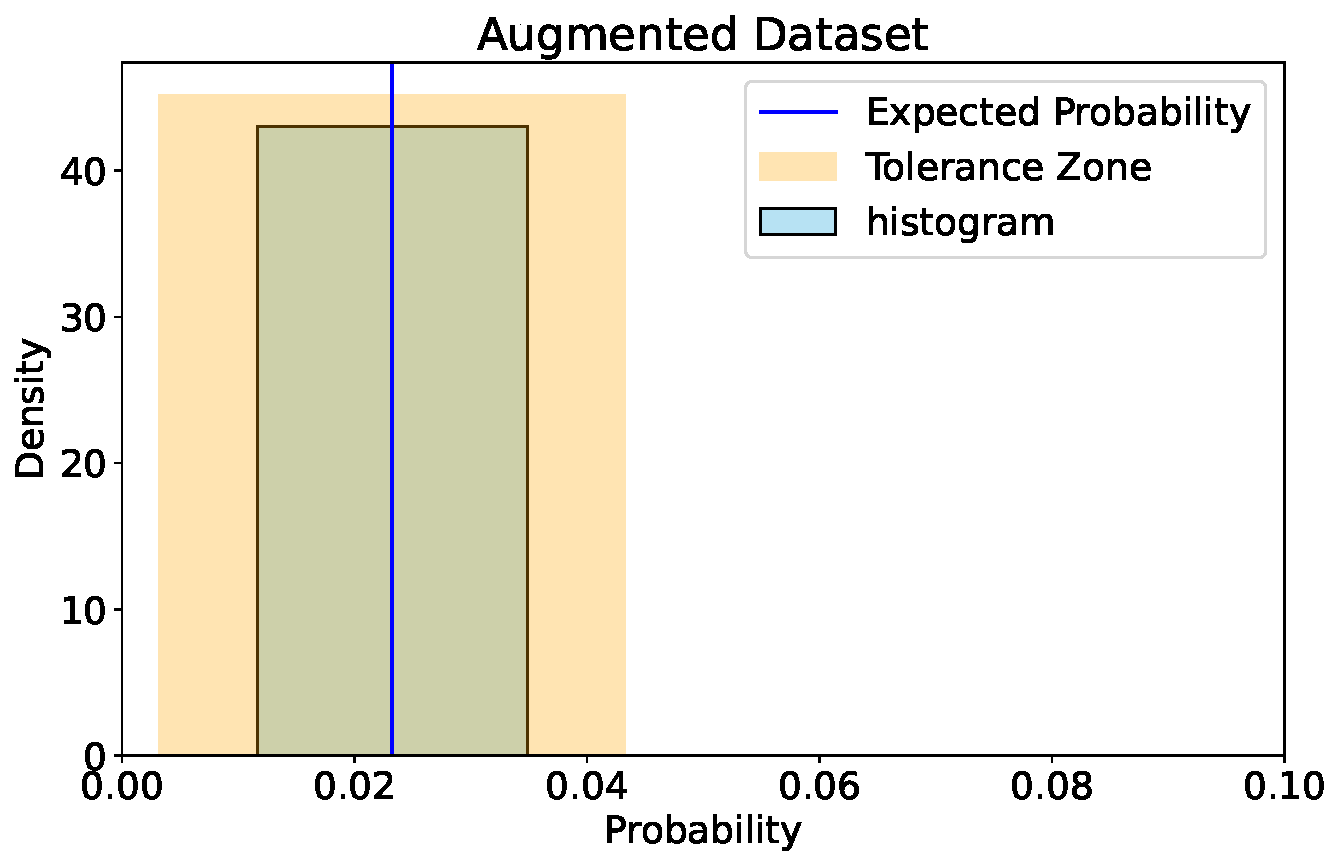
\includegraphics[width=0.95\linewidth]{img/data/evalDist/augp.pdf}
        \caption{Probability distribution, augmented.}
    \end{subfigure}
    \caption{Class distribution and class-probabilities distribution for
      Scenario~1 ($N = 39{,}209$ before and $96{,}750$ after augmentation). Augmentation flattens the class distribution and
      concentrates the probability density at $1/K \approx 0.0233$.}
    \label{fig:gtsrb:distscenario1}
\end{figure}

\begin{table}[!htbp]
\centering
\begin{tabular}{lcc}
\toprule
& \textbf{Original} & \textbf{Augmented} \\
\midrule
Dataset size $N$         & $39{,}209$             & $96{,}750$ \\
Accuracy                 & $95.17\%$              & $95.10\%$ \\
Accuracy on warning signs & $95.19\%$             & $95.40\%$ \\
Accuracy on other signs  & $89.95\%$              & $91.68\%$ \\
Accuracy gap             & $5.24$ pp              & $3.88$ pp \\
GD trust opinion $(b,d,u)$  & $(0.50, 0.11, 0.39)$   & $(0.64, 0.00, 0.36)$ \\
\bottomrule
\end{tabular}
\caption{Scenario~1 (centralized): downstream accuracy and GD trust
  opinion for the original and augmented \ac{GTSRB}.}
\label{tab:gtsrb:acc1}
\end{table}

\paragraph{Scenario~2: collaborative dataset with $M$ contributors.}
We progressively increase the number of imbalanced contributors out of $M$ and observe both the downstream accuracy and the trust opinion produced by each trust source. Downstream accuracy (\cref{fig:gtsrb:accplot}, $M = 100$) shows the expected pattern: warning-sign accuracy collapses from $83\%$ to $0\%$ as the number of imbalanced contributors grows, while accuracy on the other signs degrades gradually (the ``whole test set'' curve nearly coincides with the ``other signs'' curve because warning signs are a small fraction of the test set). The accuracy gap grows accordingly.

The trust opinions (\cref{fig:gtsrb:op}) tell a more nuanced story. The \emph{GD trust source}, applied to the union of all sub-datasets, shows belief decreasing slowly until roughly 60 imbalanced contributors out of 100, after which it drops sharply. This matches the ground truth: the warning-sign classes only leave the tolerance zone once most of their images have been removed. Its uncertainty stays constant at $\approx 0.4$ because the total dataset size $N$ barely changes (only warning-sign images are removed) and \cref{eq:gtsrb:uncertainty} depends only on $N$. The \emph{LE trust source} produces a linear decrease of belief and a symmetric increase of disbelief: each imbalanced contributor adds exactly one unit of negative evidence (\cref{eq:gtsrb:method2-evidence}), so the opinion moves deterministically from $(1, 0, 0.02)$ to $(0, 1, 0.02)$ as the sweep progresses. It is thus more sensitive than the GD trust source to the \emph{number} of problematic contributors, but blind to how much of the global distribution they actually distort, which is the complementarity discussed above.

When the same experiments are repeated with $M = 10$ contributors, the GD trust source shows essentially the same belief/disbelief curves (because $N$ and the global distribution are the same), while the LE trust source exhibits a higher residual uncertainty ($u = 2/12 \approx 0.17$) reflecting the smaller number of evidence sources $r + s = M$ in the \ac{BPQ} formula.

\begin{figure}[!htbp]
    \centering
    \begin{subfigure}{0.48\textwidth}
        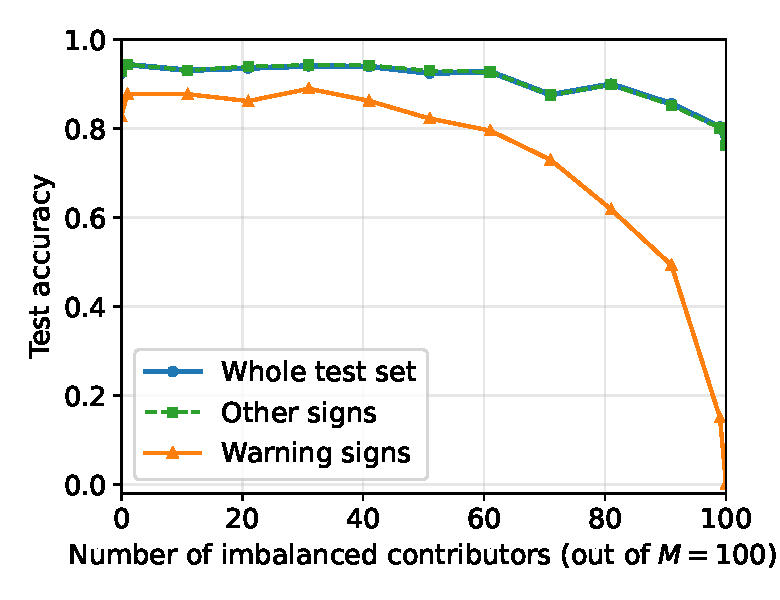
\includegraphics[width=\linewidth]{img/data/res/acc.pdf}
        \caption{Test accuracy.}
    \end{subfigure}
    \hfill
    \begin{subfigure}{0.48\textwidth}
        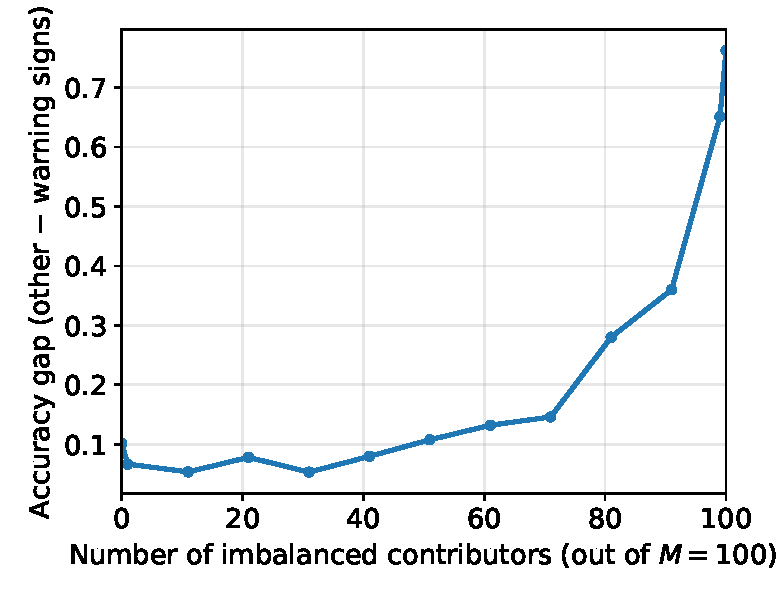
\includegraphics[width=\linewidth]{img/data/res/diff.pdf}
        \caption{Accuracy gap.}
    \end{subfigure}
    \caption{Scenario~2 ($M = 100$): test accuracy on the whole test set, on the warning signs and on the other signs, and the resulting accuracy gap, as a function of the number of imbalanced contributors. The whole-test curve nearly coincides with the other-signs curve because warning signs are a small fraction of the test set.}
    \label{fig:gtsrb:accplot}
\end{figure}

\begin{figure}[!htbp]
    \centering
    \begin{subfigure}{0.35\textwidth}
        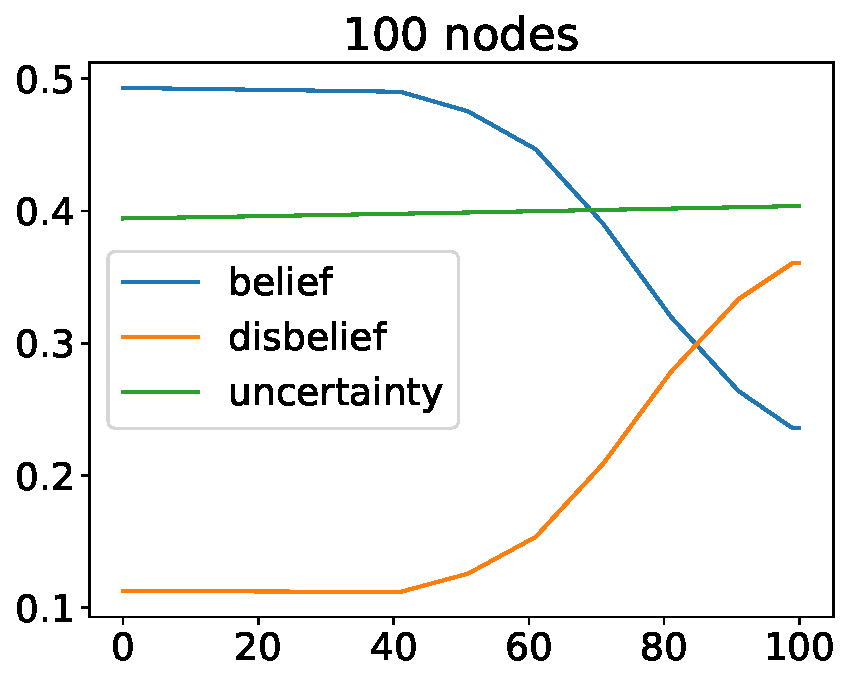
\includegraphics[width=0.95\linewidth]{img/data/res/meth1-100.pdf}
        \caption{GD trust source, $M = 100$.}
    \end{subfigure}
    \begin{subfigure}{0.35\textwidth}
        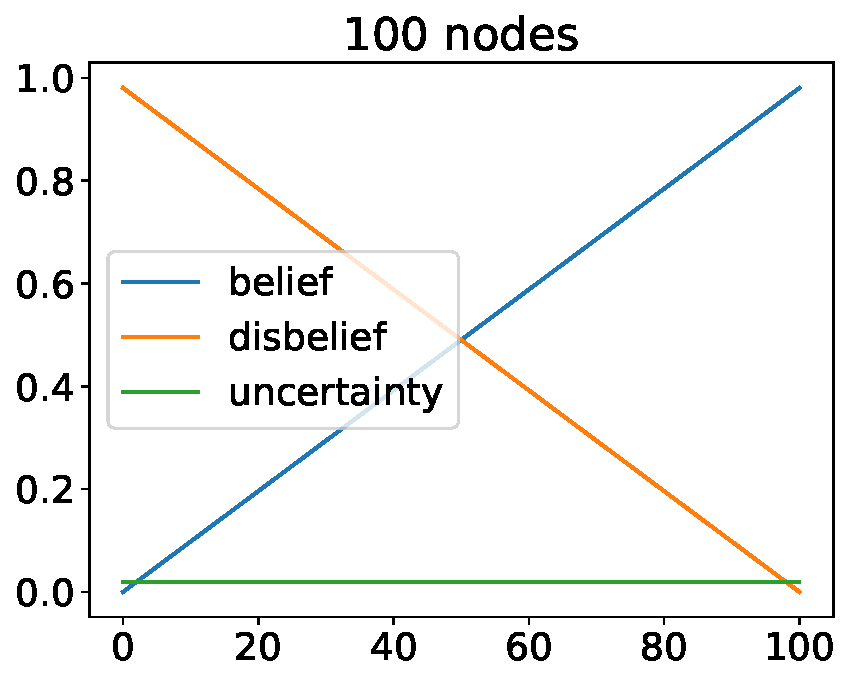
\includegraphics[width=0.95\linewidth]{img/data/res/meth2-100.pdf}
        \caption{LE trust source, $M = 100$.}
    \end{subfigure}
    \begin{subfigure}{0.35\textwidth}
        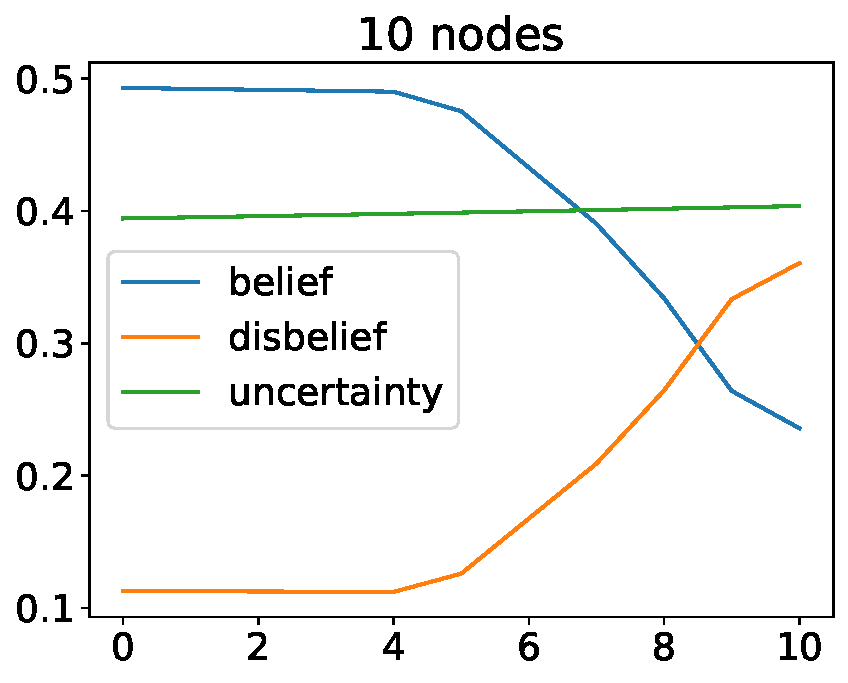
\includegraphics[width=0.95\linewidth]{img/data/res/meth1-10.pdf}
        \caption{GD trust source, $M = 10$.}
    \end{subfigure}
    \begin{subfigure}{0.35\textwidth}
        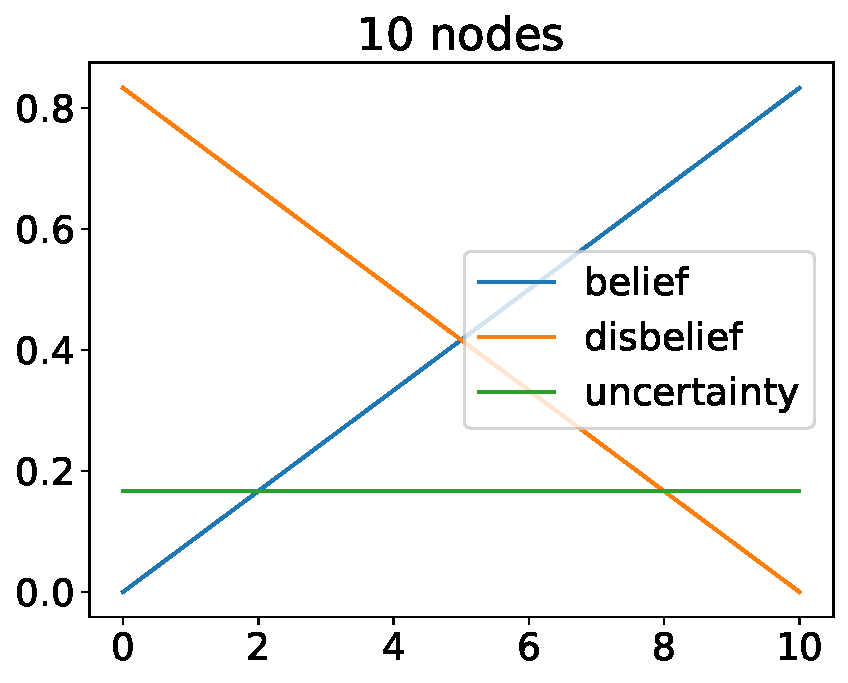
\includegraphics[width=0.95\linewidth]{img/data/res/meth2-10.pdf}
        \caption{LE trust source, $M = 10$.}
    \end{subfigure}
    \caption{Trust opinions $(b, d, u)$ produced by the GD and LE trust sources for
      $M = 10$ and $M = 100$ contributors, as a function of the number of imbalanced
      contributors ($x$-axis). The GD uncertainty is constant because the total
      dataset size $N$ is unchanged; the LE opinion moves linearly because each imbalanced contributor adds one unit of negative evidence.}
    \label{fig:gtsrb:op}
\end{figure}

\paragraph{Sensitivity to the tolerance $\eta$.}
The tolerance $\eta$ controls how strictly the GD trust source interprets balance. Too small a value penalizes minor imbalances; too large a value lets substantial imbalances pass undetected. \Cref{fig:gtsrb:eta_effect} shows belief, disbelief and uncertainty as functions of $\eta$ on the original \ac{GTSRB}. Belief rises and stabilizes as $\eta$ grows, disbelief drops correspondingly, and uncertainty stays constant as expected from \ac{CUQ}. The shaded region ($0.0185 \leq \eta \leq 0.0235$) marks a \emph{stability zone} in which the trust opinion is insensitive to small changes of $\eta$. We pick $\eta = 0.02$ for all reported experiments because it lies in the middle of this zone; this is an instance of the sensitivity-analysis recommendation of \cref{sec:dataset-trust:framework:hyperparameters}.

\begin{figure}[!htbp]
  \centering
  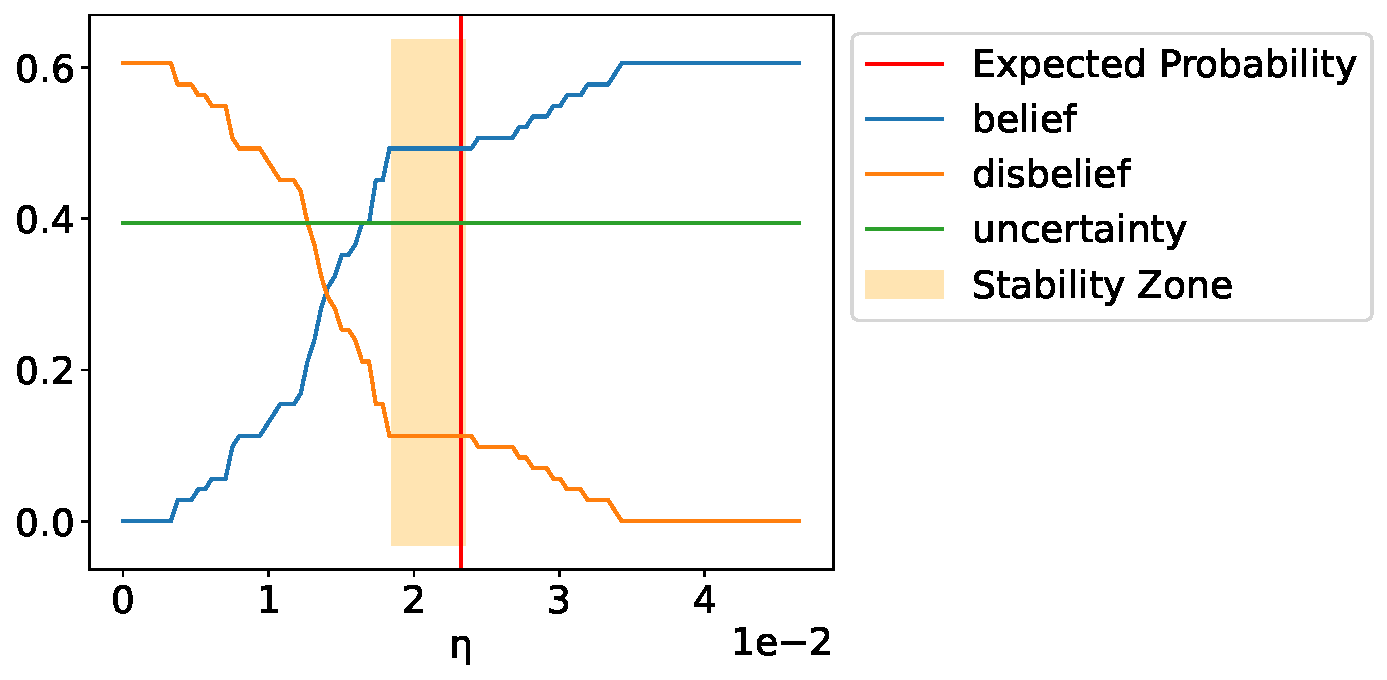
\includegraphics[width=0.7\linewidth]{img/data/eta.pdf}
  \caption{Effect of $\eta$ on the belief, disbelief and uncertainty of the GD trust source on the original \ac{GTSRB}. The red vertical line marks
    the expected probability $1/K \approx 0.02326$. The shaded region
    ($0.0185 \leq \eta \leq 0.0235$) is the stability zone in which the
    opinion is insensitive to small changes of $\eta$. Uncertainty is
    constant because the GD trust source fixes it externally via \cref{eq:gtsrb:uncertainty}.}
  \label{fig:gtsrb:eta_effect}
\end{figure}

\subsection{What this application showed}
\label{sec:gtrsb_summary}

Returning to the research question: for the proposition ``$\dataset$ is not biased with respect to class balance'', both trust sources produced opinions that track the known imbalance and its downstream effect. In Scenario~1 the GD opinion separated the original dataset (eight classes outside the tolerance zone, $d = 0.11$) from the balanced one ($d = 0$), in line with the reduction of the accuracy gap. In Scenario~2 both opinions moved toward disbelief as contributors became imbalanced and the warning-sign accuracy collapsed, but along different curves that reflect what each trust source can observe.

The two trust sources answer the same proposition by different routes and have complementary strengths. The GD trust source requires the global class-probabilities distribution and is the natural choice when the dataset is centralized and observable. The LE trust source only requires one scalar per contributor and is therefore the natural choice in collaborative or federated settings where class counts cannot be shared, at the price of the complementarity blind spot discussed in \cref{sec:dataset-trust:applications:gtsrb:method2}. They also illustrate two different quantification schemes: the GD trust source fixes uncertainty externally via sample complexity, which is appropriate when the dataset size is the bottleneck of the assessment's confidence; the LE trust source lets uncertainty shrink as more contributors provide evidence, which is appropriate when the unit of evidence is one local assessment per contributor. The same proposition can therefore be assessed under \ac{CUQ} or \ac{BPQ} depending on whether ``more evidence'' means ``more data'' or ``more contributors''.

Two caveats apply. Class imbalance is not always a defect: in some applications it faithfully reflects the deployment-time class frequencies, and forcing balance would degrade rather than improve the model. A natural extension of the GD trust source replaces the uniform expected probability $1/K$ with a deployment-derived target distribution, preserving the rest of the procedure. And the sample-complexity bound used to set $U$ is conservative, so the absolute level of uncertainty ($\approx 0.4$) should be read as a relative scale across datasets rather than as a calibrated probability.

\FloatBarrier

% ==============================================================
\section{Annotation Stage, Entry Level: Labeling accuracy on \\CIFAR-10H}
\label{sec:dataset-trust:applications:cifar10h}

\begin{mdframed}[backgroundcolor=blue!4, linewidth=0pt]
\textbf{Position in the design space.}

$\propP$ = accuracy (of labels);\quad
$\propS = \{\textsc{annotation}\}$;\quad
$\propG$ = entry;\

\textbf{Quantification:} \ac{BPQ} (evaluated), \ac{EWQ} (discussed).\quad

\textbf{Purpose:} evaluation.\quad \textbf{Published in:}~\cite{trust-aidatatrust}.
\end{mdframed}

\paragraph{Purpose and research question.}
The third application evaluates the framework at the \emph{entry} granularity, where each individual label is a trust proposition of its own. It was chosen because labeling accuracy is the dataset property with the most direct effect on a supervised model and because CIFAR-10H offers something rare: for every image, about fifty independent human labels, so that the disagreement between annotators, which is the evidence the framework uses, is directly observable and can be manipulated. The research question is: \emph{do per-entry opinions derived from annotator agreement identify genuinely ambiguous items, and does their uncertainty respond correctly to the amount of annotation available for each item?} The application also shows how the same construction extends to the annotators themselves, which connects the dataset assessment to the trust-discounting operator of \cref{chap:rw}.

\paragraph{Dataset and annotation scenario.}
CIFAR-10H~\cite{peterson2019human} re-annotates the $10{,}000$ images of the CIFAR-10 test set~\cite{krizhevsky2009learningcifar} (ten object classes such as \emph{airplane}, \emph{cat}, \emph{truck}). Each image was shown to about $51$ crowdworkers recruited on Amazon Mechanical Turk ($2{,}571$ workers in total, $511{,}400$ labels), each of whom chose one of the ten classes; workers labeled 200 images each, with attention checks. The scenario is thus the standard one of crowdsourced labeling: several independent, non-expert annotators label the same item, and the dataset curator has to decide on one label per item. In CIFAR-10H, as in most crowdsourcing pipelines, that decision is taken by \emph{majority vote} over the annotators; the majority label is the one we assess. The original CIFAR-10 label is also available and agrees with the majority label for the vast majority of images, which is why the dataset is a good testbed: disagreement among annotators concentrates on genuinely ambiguous images (e.g., a cat that looks like a dog) rather than on random noise~\cite{peterson2019human}.

\paragraph{Trust proposition.}
For each image $x$, the proposition is \emph{``the decision label $y^\prime$ for $x$ is accurate,''} where $y^\prime$ is the majority label. Each image is assessed independently, producing a per-entry opinion $\omega_{x} = (b_{x}, d_{x}, u_{x})$. The set of per-entry opinions can be lifted into a dataset-level opinion on labeling accuracy with the cross-granularity mechanisms of \cref{sec:dataset-trust:formal:granularity}.

\subsection{Trust source: divergence to the decision label}
\label{sec:dataset-trust:applications:cifar10h:source}

The trust source operates at the level of individual annotators. For each annotator $j$ of instance $x$, we compute a divergence score $d_j(x)$ that measures how far the annotator's response is from the decision label $y^\prime$. For categorical annotations, $d_j(x) = 0$ when the annotator agrees with $y^\prime$ and $d_j(x) = 1$ otherwise; for probabilistic annotations, \ac{KL} divergence or cross-entropy between the annotator's distribution and $y^\prime$ is a natural choice; for free-text annotations, semantic distance (e.g., cosine distance between embeddings) plays the same role.

A divergence threshold $\delta$ separates evidence supporting the proposition from evidence against it:
\begin{equation}
r_x = \big|\{j : d_j(x) \leq \delta \}\big|,
\qquad
s_x = \big|\{j : d_j(x) > \delta \}\big|.
\label{eq:cifar10h:evidence}
\end{equation}

The threshold $\delta$ can be set in several ways depending on the annotation modality and on what reference information is available.

\noindent \emph{By edge-case construction}, $\delta$ is set to the divergence that an \emph{edge-acceptable} annotation would produce relative to the decision label: that is, an annotation that is the most distant response still considered acceptable for the given label, by analogy with the edge-acceptable distribution used to set the threshold of the LE trust source in the \ac{GTSRB} application (\cref{sec:dataset-trust:applications:gtsrb:method2}).

\noindent \emph{By domain policy}, $\delta$ is fixed by external requirements, e.g., $\delta = 0$ for categorical labels (strict agreement) and $\delta = 0.1$ for soft labels.

\cref{alg:cifar10h:opinions} summarizes the construction of per-entry opinions.

\begin{algorithm}[!htbp]
\caption{Per-entry opinion construction from annotations}
\label{alg:cifar10h:opinions}
\label{alg:opinions}
\begin{algorithmic}[1]
\Require Annotations $\{y_j(x)\}$ or $\{p_j(x)\}$, decision label $y^\prime$,
threshold $\delta$, prior weight $W$
\For{each instance $x$}
  \State $r_x \leftarrow |\{j : \mathrm{divergence}(y_j(x), y^\prime) \leq \delta \}|$
  \State $s_x \leftarrow |\{j : \mathrm{divergence}(y_j(x), y^\prime) > \delta \}|$
  \State $b_x \leftarrow r_x / (W + r_x + s_x)$
  \State $d_x \leftarrow s_x / (W + r_x + s_x)$
  \State $u_x \leftarrow W / (W + r_x + s_x)$
  \State Output opinion $\omega_x = (b_x, d_x, u_x, a)$
\EndFor
\end{algorithmic}
\end{algorithm}

\paragraph{Quantification schemes: \ac{BPQ} and \ac{EWQ}.}
The trust source produces evidence counts $(r_x, s_x)$ that grow with the number of annotators $n = r_x + s_x$ of instance $x$. This makes two quantification schemes natural. \ac{BPQ}, with prior weight $W$, gives uncertainty $u_x = W / (W + n)$: residual uncertainty decreases as more annotators contribute, which is the desired behavior when annotation volume varies across instances. \ac{EWQ} additionally assumes that each annotation comes with its own uncertainty weight. It is relevant when annotators self-report a confidence score alongside their label, or when external metadata provides a per-annotation reliability proxy (e.g., annotation duration). Where \ac{BPQ} lets the \emph{amount} of evidence drive uncertainty, \ac{EWQ} lets the \emph{quality} of each piece of evidence drive it. CIFAR-10H records neither confidence nor duration, so only \ac{BPQ} is evaluated below.

\paragraph{Worked example.}
Consider an instance $x$ annotated by $50$ crowdworkers, of whom $46$ agree with the decision label and $4$ disagree, with $\delta = 0$ and $W = 2$. \cref{eq:cifar10h:evidence} gives $r_x = 46$, $s_x = 4$, and \ac{BPQ} gives:
\begin{equation}
b_x = \tfrac{46}{52} \approx 0.885,\quad
d_x = \tfrac{4}{52} \approx 0.077,\quad
u_x = \tfrac{2}{52} \approx 0.038.
\end{equation}
The opinion captures three qualitatively different signals simultaneously: high belief reflecting strong agreement, residual disbelief reflecting genuine disagreement among annotators, and low uncertainty reflecting that the evidence base is large.

\paragraph{Annotator-level extension.}
The same construction applies to a different entity: the annotators themselves. For annotator $j$, partitioning $j$'s responses across all the items $j$ labeled into agreements and disagreements with the corresponding decision labels yields evidence counts $(r_j, s_j)$ for the proposition \emph{``annotator $j$ is reliable''}. Applying \ac{BPQ} to $(r_j, s_j)$ produces a per-annotator opinion $\omega_j$ on the same $(b, d, u)$ scale as the per-entry opinions.

This construction implicitly assumes that more than half of the annotators are honest and competent: the decision label $y^\prime$ is taken as the reference against which each annotator is judged, so the resulting reliability opinion is only meaningful if the procedure that produced $y^\prime$ is itself reliable. If $y^\prime$ is set by majority vote, the assumption is that the majority of annotators is correct on most items. In settings where this fails (e.g., adversarial annotators colluding to flip the majority on targeted items), $\omega_j$ would conflate genuine reliability with mere conformity to a corrupted reference.

\paragraph{Connection to trust discounting.}
The per-annotator opinion is exactly the \emph{referral} trust opinion expected by the trust-discounting operator of \cref{subsec:TD_operators}. In the terminology of \cref{def:two_edge_discounting}, the curator $A$ holds a referral opinion $\omega^A_j = \omega_j$ about annotator $j$, and annotator $j$ holds a functional opinion about the proposition ``$y^\prime$ is accurate for $x$'': a categorical vote is the dogmatic opinion $\omega^j_x = (1, 0, 0)$ if $j$ agrees with $y^\prime$ and $(0, 1, 0)$ otherwise. Two-edge discounting gives the curator's opinion via $j$,
\[
\omega^{[A;j]}_x = \omega^A_j \otimes_{TE} \omega^j_x =
\begin{cases}
(P_j,\ 0,\ 1 - P_j) & \text{if } j \text{ agrees with } y^\prime,\\
(0,\ P_j,\ 1 - P_j) & \text{otherwise},
\end{cases}
\]
where $P_j = b_j + a\,u_j$ is the projected probability of $\omega_j$, and the per-entry opinion is the cumulative fusion $\bigoplus_j \omega^{[A;j]}_x$ over the annotators of $x$. In evidence terms, this replaces the plain counts of \cref{eq:cifar10h:evidence} by counts weighted by the annotators' reliability, $r_x = \sum_{j \text{ agrees}} P_j$ and $s_x = \sum_{j \text{ disagrees}} P_j$: a fully reliable annotator contributes one unit of evidence, an unreliable one contributes less, and the difference is turned into uncertainty rather than discarded. The labeling-accuracy assessment thus becomes a two-level instantiation of the General Methodology: the proposition ``$y^\prime$ is accurate'' is supported by referral evidence from annotators whose own reliability is an assessable proposition.

\subsection{Experimental evaluation}
\label{sec:dataset-trust:applications:cifar10h:eval}

We evaluate the trust source on the full CIFAR-10H ($10{,}000$ images, about $51$ annotations each). The decision label $y^\prime$ of each image is its majority label, the divergence threshold is $\delta = 0$ (strict agreement) and the prior weight is $W = 2$.

\Cref{fig:cifar10h:masses} compares the empirical distribution of $(b_x, d_x, u_x)$ over the $10{,}000$ images in two settings: the full dataset, and a \emph{cropped} variant in which each image is reduced to $10$ annotations by removing responses from the majority label only, so that the cropped set retains all minority annotations while reducing the dominant agreement signal. This manipulation is designed to answer the second half of the research question: it changes the amount of evidence per item without changing which items are ambiguous.

Two effects are visible. First, on the full dataset belief concentrates near $1$ and uncertainty near $0$: with about $50$ annotators per image, $u_x = W / (W + 50) \approx 0.04$ regardless of the agreement ratio. This high apparent confidence is partly an artifact of evidence saturation rather than a genuine signal of label quality, and it is the correct behavior of \ac{BPQ}: fifty independent votes \emph{are} a lot of evidence about a majority label. The items that matter are the outliers of the belief box plot, i.e., the images on which a sizeable minority of annotators disagreed; these are, by construction, the images on which CIFAR-10H's annotators disagree, which~\cite{peterson2019human} report to be visually ambiguous rather than randomly mislabeled. Second, the cropped setting redistributes mass across the three components: disbelief becomes visible for items with annotator disagreement, and uncertainty rises mechanically to $u_x = W / (W + 10) \approx 0.17$. The opinions are now informative about the actual difficulty of each item, with controversial instances showing simultaneously low belief and high disbelief, while unanimous ones keep $d_x = 0$.

\begin{figure}[!htbp]
    \centering
    \begin{subfigure}[b]{0.49\textwidth}
        \centering
        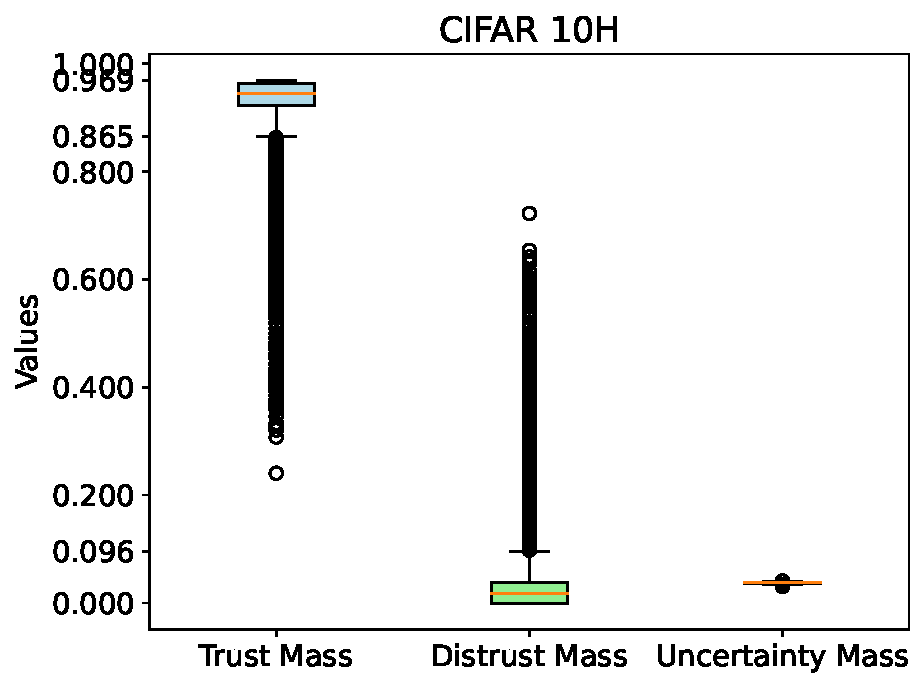
\includegraphics[width=\textwidth]{img/data/CIFAR_10H.pdf}
        \caption{Full CIFAR-10H ($\approx 50$ annotators per item).}
    \end{subfigure}
    \hfill
    \begin{subfigure}[b]{0.49\textwidth}
        \centering
        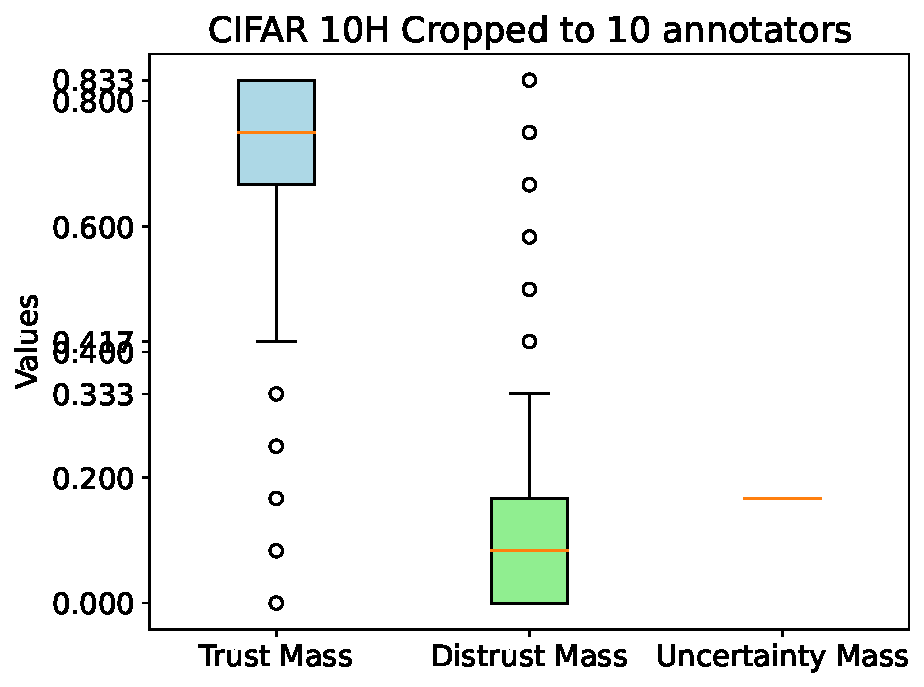
\includegraphics[width=\textwidth]{img/data/CIFAR_10H_Cropped.pdf}
        \caption{Cropped to $10$ annotators per item by removing majority-label responses.}
    \end{subfigure}
    \caption{Box plots of belief, disbelief and uncertainty over the $10{,}000$ images of
      CIFAR-10H. The full dataset shows high belief and low
      uncertainty driven primarily by evidence saturation. The cropped
      setting redistributes mass across the three components and surfaces
      genuine annotator disagreement.}
    \label{fig:cifar10h:masses}
\end{figure}

\subsection{What this application showed}
\label{sec:dataset-trust:applications:cifar10h:discussion}

Returning to the research question: the per-entry opinions single out the ambiguous images through their disbelief mass, and their uncertainty responds to the amount of annotation exactly as \ac{BPQ} prescribes ($0.04$ with $50$ annotators, $0.17$ with $10$), independently of the agreement ratio. This separation is what a scalar agreement rate cannot provide: an image with $9$ agreeing annotators out of $10$ and an image with $45$ out of $50$ have the same agreement rate but different opinions, $(0.75, 0.08, 0.17)$ versus $(0.87, 0.10, 0.04)$, the second being held with more confidence.

Per-annotator opinions $\omega_j$ can in turn be used to filter unreliable contributors, to reweight their evidence through the discounting construction above, or to drive targeted re-annotation. This application covers the annotation stage at entry granularity, exercises \ac{BPQ}, discusses where \ac{EWQ} would apply, illustrates the cross-granularity composition of \cref{sec:dataset-trust:formal:granularity}, and connects to the trust-discounting operator via the annotator-level extension. Together with the \ac{GTSRB} application, it covers the two canonical routes to a dataset-level assessment: direct global evidence (\ac{GTSRB}) and lifted entry-level evidence (CIFAR-10H).

\noindent \cref{tab:dataset-trust:applications-summary} summarizes the position of the three applications in the design space.

\begin{table}[!htbp]
  \centering
  \small
  \renewcommand{\arraystretch}{1.2}
  \begin{tabular}{@{}llll@{}}
    \toprule
     & \textbf{COMPAS} & \textbf{GTSRB} & \textbf{CIFAR-10H} \\
    \midrule
    Property $\propP$        & overall trustworthiness & representativeness & labeling accuracy \\
    Stage(s) $\propS$        & all four                & sampling           & annotation \\
    Granularity $\propG$     & dataset                 & dataset            & entry \\
    Quantification           & \acs{BPQ}               & \acs{CUQ}, \acs{BPQ} & \acs{BPQ} (\acs{EWQ} discussed) \\
    Purpose                  & illustration            & evaluation         & evaluation \\
    \midrule
    Dataset source           & ProPublica~\cite{angwin2016machine} & \cite{stallkamp2012man} & \cite{peterson2019human} \\
    Published in             & this dissertation       & \cite{10.1007/978-3-032-19096-3_17} & \cite{trust-aidatatrust} \\
    \bottomrule
  \end{tabular}
  \caption{Position of each application in the three-axis design space of
    \cref{sec:dataset-trust:framework:design-space}, the quantification scheme it exercises, its purpose, the origin of the dataset and the publication in which it first appeared.}
  \label{tab:dataset-trust:applications-summary}
\end{table}

\FloatBarrier

% ==============================================================
\section{Summary \& Conclusions} \label{sec:dataset-trust:summary}

This chapter introduced a framework for assessing the trustworthiness of \ac{AI} training datasets by specializing the general methodology of \cref{chap:Trust_method}. Its central claim is that dataset trustworthiness should be treated not as a single score, but as a structured assessment defined by three dimensions: the property assessed, the lifecycle stage from which evidence is collected, and the granularity at which it applies.

The framework rests on three artifacts. First, the lifecycle decomposition (sampling, collection, annotation, processing) and the trust-source catalogue fix the \emph{structure} of an assessment: a two-level trust expression whose leaves are trust sources selected by property, stage and granularity. Second, the quantification procedure turns the value of a trust source into evidence (through threshold-based normalization and an evidence strength) and evidence into an opinion (through \ac{BPQ}, \ac{EWQ} or \ac{CUQ}), with explicit, reportable hyperparameters. Third, the cross-granularity composition mechanisms (opinion composition and evidence lifting) let evidence collected at feature or entry level support entry- or dataset-level propositions.

Three applications instantiated the framework. \ac{COMPAS} illustrated multi-stage composition on a real tabular dataset and showed that the stage-level opinions distinguish a stage weakened by negative evidence from a stage that merely lacks evidence. \ac{GTSRB} evaluated two trust sources for class balance against a known, controllable imbalance and its effect on a \ac{CNN}, in centralized and federated settings, and showed that the same proposition can be quantified under \ac{CUQ} or \ac{BPQ} depending on what is observable. CIFAR-10H evaluated entry-level opinions against directly observable annotator disagreement and showed that belief, disbelief and uncertainty separate ambiguity from lack of annotation.

The framework provides richer decision support than scalar metrics. An opinion $(b, d, u)$ distinguishes supporting evidence, contradicting evidence, and uncertainty. This enables auditors to differentiate between lack of evidence and conflicting evidence, two situations requiring different actions, making the framework a diagnostic tool rather than a pass/fail measure.

\paragraph{Limitations.}
Three limitations remain. First, the trust-source catalogue is not exhaustive: it lists the trust sources considered in this thesis, and applying the framework to a concrete system will typically require defining additional ones, which the catalogue accommodates as long as they are placed at a stage, a risk category and a granularity. Second, the hyperparameters ($\tau_m$, $A_m$, $L_m$, $K_m$, $W$, $U$) must be set by the analyst. \cref{sec:dataset-trust:framework:hyperparameters} gives guidance (requirements or expert elicitation for thresholds, with sensitivity analysis as a safeguard; uniform $K_m$ unless source authority differs; $W = 2$ unless evidence is noisy), and the $\eta$ sensitivity analysis of \cref{sec:dataset-trust:applications:gtsrb:eval} shows that partial calibration is feasible, but the assessment remains only as meaningful as these choices, which is why they must be reported with it. Third, the lifecycle stages enter the conjunction of \cref{eq:dataset-trust:lifecycle-decomposition} with equal weight, whereas a task may warrant weighting them differently: for a fairness audit of a hiring dataset the annotation stage (who assigned the outcome labels) dominates, whereas for a sensor-fusion dataset the collection stage (calibration and drift) does. Such weighting can be expressed within \ac{SL} by discounting the stage-level opinions with a task-dependent referral opinion before the conjunction, which is left to future work.

\paragraph{Relation to the Trust Propagation Module.}
The framework outputs trust opinions at dataset, entry or feature granularity. These are the inputs of the Trust Propagation Module of \ac{PaTAS}, presented and evaluated in \cref{chap:patas}, which operates on per-feature trust opinions. A coarser-grained (dataset- or entry-level) opinion can be replicated at the feature level, enabling propagation through the model parameters during training. At inference time, the same trust sources applied to the features of an individual input yield per-feature opinions, which are propagated through the network to produce an output trust opinion. Replicating a dataset-level opinion onto every input, however, gives every input the same trust regardless of its individual quality, which limits the value of per-instance trust evaluation at inference. Input-level assessment should therefore \emph{add} entry- or feature-level trust sources computed on the individual input to the dataset-level opinion, rather than replace one by the other: the dataset-level opinion captures what the model was trained on, the input-level opinion what it is being asked about, and both enter the propagation.

Finally, while the training-dataset assessment and the inference-time input assessment may share the same trust property, they do not need to rely on the same trust sources. The analyst is free to use different trust sources for the two, as long as both address the same underlying proposition. For instance, dataset-level accuracy may be supported by sensor-consistency scores computed across the training set, while input-level accuracy at inference time may be supported by an out-of-range check or a per-sensor confidence score applied to the individual input.

\chapter{Trust Propagation in \aclu{NN}}
\label{chap:patas}
The previous \cref{chap:ovl} presented the overall architecture of \ac{PaTAS}, highlighting its two main components: (i) the assessment of trust in the data, and (ii) the propagation of trust through the model, from the training data to the learned parameters and from the input to the output via these parameters. While the trustworthiness of the data was addressed in the preceding chapter, this chapter focuses on the second component, namely the propagation of trust within \aclu{NN}. In particular, it details how trust, initially derived from the dataset, is integrated into the model parameters during training and subsequently propagated from the input to the output during inference. This chapter formalizes the mechanisms that enable consistent and interpretable trust propagation across the different stages of the learning process, providing the operational core of the \ac{PaTAS-TP} framework.

An interactive simulator demonstrating the trust propagation mechanisms described in this chapter is available at \url{https://ouatt-isma.github.io/patas_simulator}.
\begin{chapterlink}
\textbf{Connection with the preceding chapters.} This chapter builds directly on two prior contributions of the thesis: the \aclu{TNA-SL} foundations introduced in \cref{chap:rw}, which define how the \ac{SL} operators are used to combine trust opinions over \aclp{DSPG}, and the dataset-trust quantification methodology developed in \cref{chap:dataset-trust}, which produces the feature-, instance-, and label-level trust opinions consumed here as inputs ($T(x)$, $T(y)$). The present chapter closes the loop by specifying how these \emph{dataset-derived opinions} are transformed into \emph{parameter trust} during training and \emph{input trust} into \emph{output trust} during inference, thereby answering \ac{RQ}~3.
\end{chapterlink}

\section{Introduction}
The preceding chapter addressed the first component of \ac{PaTAS}: the quantification of trustworthiness in training datasets. It established that trust in a dataset can be assessed at multiple granularities, from global distributional properties to individual feature-level reliability, and provided formal tools for computing \ac{SL} opinions over data quality. However, quantifying dataset trustworthiness is only a prerequisite. The central challenge, as formulated in \ac{RQ}~3, is to propagate this trust through the learning and inference processes, such that the reliability of a prediction can be systematically traced back to the reliability of both the data and the parameters from which it originates.

As discussed in \cref{chap:rw}, the trustworthiness of a \aclu{NN} output cannot be treated as a static property of the model alone. During training, model parameters are updated through gradient-based optimization driven by labeled data. If this data is noisy, biased, or corrupted, the resulting parameter updates inherit these deficiencies, embedding unreliability directly into the learned model. During inference, inputs are transformed through successive layers parameterized by these learned weights; consequently, unreliability originating from either the input or the parameters may propagate and accumulate throughout the network, ultimately affecting the final prediction. Standard performance metrics such as accuracy fail to capture this phenomenon, as they conflate correctness with reliability. A model may achieve high accuracy on a poisoned or biased dataset while producing predictions that remain fundamentally untrustworthy.

Existing approaches to trust and uncertainty propagation in \acp{NN}, reviewed in \cref{sec:trust_uq}, address aspects of this problem but leave important gaps. Uncertainty propagation methods, such as those of Monchot et al.~\cite{pmlr-v202-monchot23a} and Astudillo and Neto~\cite{astudillo2011propagation}, model the transmission of statistical variability through network layers, but treat uncertainty primarily as a distributional property of the input. As such, they do not capture the joint influence of dataset reliability and parameter trustworthiness on the final prediction. The DeepTrust framework of Cheng et al.~\cite{10.3389/frai.2020.00054} is more closely related, as it propagates dataset-level trust opinions through a \ac{NN} to derive a global model trust estimate. However, as discussed in \cref{sec:sl_approaches}, DeepTrust's formulation leaves several theoretical questions open. Its mapping of \ac{NN} addition to \ac{SL} fusion and multiplication to SL opinion multiplication mixes operators from distinct algebraic domains, since fusion operates over agents' opinions while multiplication operates over variables, without a principled justification for this correspondence. Furthermore, its trust computation is specified only at the output layer, and the mechanism does not admit a straightforward extension to intermediate layers of deep architectures. As a result, while DeepTrust motivates the use of \ac{SL} for trust assessment in \acp{NN}, the semantics of its propagation in deeper settings remain underspecified.

This chapter provides a formal and operational answer to \ac{RQ}~3 by introducing a principled framework for trust propagation in \acp{NN}. Building on the foundations of \ac{SL} and the optimized trust inference mechanisms introduced in \cref{chap:tnasl}, we model trust as a transitive, structure-aware, and evidence-driven quantity that propagates through the network in parallel with standard \ac{NN} computation. The proposed framework integrates two complementary sources of trust: (i) the reliability of input features at inference time, and (ii) the reliability of model parameters, which themselves are derived from the trustworthiness of the training dataset. Importantly, this propagation is performed without modifying the underlying \ac{NN}, thereby preserving compatibility with existing architectures. Methodologically, \ac{PaTAS-TP} is a \emph{white-box} framework: it exploits the internal structure of the \ac{NN}, namely its layer topology, parameters, and activation paths, to compute trust at each intermediate computation rather than treating the model as an opaque input--output mapping. This places \ac{PaTAS-TP} in direct contrast with the black-box calibration approach of \cref{chap:bb}.

More specifically, this chapter introduces the following contributions. First, we define a parallel trust computation mechanism based on Trust Nodes and Trust Functions, which mirror the structure of \ac{NN} computations and enable consistent trust propagation using \ac{SL} operators such as fusion and discounting. Second, we propose a parameter-trust update mechanism that estimates the reliability of learned parameters during training by leveraging gradient information, features trust, and label trust, thereby aligning parameter trust with the learning dynamics; the gradient-stability threshold it relies on is given a scale-tied, task-relative formulation that removes its only tuning burden. Third, we introduce the \ac{IPTA}, a context-aware mechanism that computes instance-specific trust scores by exploiting the activation paths involved in the prediction, and generalize it to convolutional architectures through activity-weighted path conditioning. Fourth, we instantiate the input-trust route with a conformity-based construction that derives per-feature opinions from training-data statistics, and compose it with the path trust into a single per-sample score. Finally, we evaluate the framework empirically, on controlled degradations of three datasets and in a comparative battery against established uncertainty and detection baselines. The evaluation is designed to attribute rather than to aggregate. It shows that the detection of inputs which violate the training distribution is carried by the input-side conformity opinions, which on their own match or exceed the composed per-sample score on most detection tasks; that trust propagation adds detection signal mainly for corruptions that preserve the input marginals; and that the contribution unique to the propagation mechanism is on the model side, namely the class-level localisation of training-data poisoning and a training-quality signal that requires no test data. The trust estimates are stable under training and consistent with the theoretical properties established here, within two expressiveness limits that are stated up front in \cref{sec:dnn_trust}: the trust functions do not see the sign or magnitude of weights and activations, and output disbelief can only originate from input disbelief.

The remainder of this chapter is organized as follows. \Cref{sec:trust_foundations} introduces the formal foundations of trust-aware \ac{NN} computation and defines the parallel trust function. \Cref{sec:tp_arch_ovvw} presents the \ac{PaTAS-TP} architecture, decomposing it into four functional modules: Trust Feedforward, Output-Trust Aggregation, \ac{GenIPTA}, and Parameter-Trust Update. \Cref{sec:perceptron} illustrates the core mechanisms of the Trust Feedforward through a simple perceptron example. \Cref{sec:dnn_trust} generalizes these mechanisms to deep \acp{NN} by introducing the Trust Function and layer-wise propagation. The propagation is defined neuron by neuron and each step only needs the incoming opinions of one neuron, so it is well defined for any architecture and does not rely on the \ac{DSPG} property; the \ac{DSPG}-based analysis of \cref{chap:tnasl} remains relevant for alternative designs that build a single trust network across paths of neurons, and for the dataset trust assessment of \cref{chap:dataset-trust}. The same section states the independence assumption behind the fusion step, the fusion operator actually used, and the expressiveness limits of the trust functions. \Cref{sec:param_update} details the Parameter-Trust Update mechanism that refines trust in learned parameters during training. \Cref{sec:ptastheory} establishes theoretical properties of the framework, including the stability of the parameter-trust update and its operator-specific limits. \Cref{sec:inference-trust} instantiates the per-sample trust assessment used at inference time: the conformity-based input-trust construction, its a-priori applicability diagnostics, and the composed trust score. \Cref{sec:patas-tp-evaluation} provides comprehensive experimental validation of increasing complexity, from controlled degradations on three datasets to a comparative evaluation against uncertainty and detection baselines. Finally, \cref{sec:patas-discussion} discusses key findings and practical implications, and \cref{sec:patas-tp-conclusion} concludes the chapter.

\section{Foundations of Trust Propagation in \aclu{NN}s}
\label{sec:trust_foundations}
This section introduces the formal structures needed to represent and propagate trust alongside standard \ac{NN} computation, namely during feedforward and backpropagation.

\subsection{Trust Representation in \aclu{NN}}
As established previously, a \aclu{SeqNN} $f_\Theta$ with parameters $\Theta = (\mathbf{W}, \mathbf{b}, \phi)$ defines a structured computational graph that maps an input $x$ to an output $y'$ through a sequence of layer-wise transformations:
\[
y' = f_\Theta(x).
\]

Rather than reintroducing the full formulation, we emphasize that this computation induces a \ac{DAG} in which information flows from input features to output predictions through intermediate activations and parameters. Trust propagation inherits the compositional structure of this computation: just as numerical values flow through the network from inputs to outputs via intermediate activations and parameters, trust assessments can be propagated along the same directed dependencies.

To enable trust-aware reasoning, we associate trust opinions with the key components of the \ac{NN}. Specifically, we consider:
\begin{itemize}
    \item \textbf{Input Trust:} A trust assessment $T(x)$ assigned to the input $x$, defined at feature-level granularity as introduced in \cref{chap:dataset-trust}.

    \item \textbf{Label Trust}: A trust assessment $T(y)$  assigned to the label $y$ associated with a training sample $(x,y) \in \mathcal{D}$, reflecting the reliability of the annotation process. It serves as a conditioning factor in the calculation of trust in the learnable parameters during training.

    \item \textbf{Parameter Trust:} A trust assessment $T(\theta)$ for each model parameter $\theta \in \Theta$, reflecting the reliability of learned parameters as a function of the training data and learning process.
    
    \item \textbf{Output Trust:} A trust assessment $T(y')$ associated with the model output $y'~=~f_\Theta(x)$.
\end{itemize}
% \noindent Trust in values are represented using \ac{SL} binomial opinions: \((t, d, u)\).

\noindent The central problem addressed in this chapter is therefore twofold. During training, trust must flow from the dataset, specifically from the reliability of input features and labels, into the learned model parameters, so that data quality is reflected in the resulting weights. During inference, trust must then be carried forward from the input features and the trust parameters to the model output, following the same computational dependencies that govern the forward pass. In both cases, propagation is understood as a transitive relationship: the trustworthiness of a downstream component is conditioned on, and inherits from, the trustworthiness of the upstream components on which it depends.

\subsection{Parallel Trust Function}
To address this problem, we introduce the notion of a \emph{parallel trust function}, which mirrors the structure of the \ac{NN}.

\begin{definition}[Parallel Trust Function]
Let $f_\Theta$ represent \ac{NN} with parameters $\Theta$, and let $T(x)$ denote trust assessments over the input of the \ac{NN}. The \emph{parallel trust function}, denoted $Pf_\Theta$, is defined as:
\[
Pf_\Theta(T(x)) = T(f_\Theta(x)),
\]
where $T(f_\Theta(x))$ is the resulting trust opinion on the output of the \ac{NN}, reflecting both the trust assigned to the input features and the trust encoded in the learned parameters $\Theta$.
\end{definition}

The parallel trust function is constructed to satisfy two key principles:
\begin{itemize}
    \item \textbf{Structural Consistency:} The trust propagation mechanism mirrors the computational structure of the \ac{NN}. Each transformation in $f_\Theta$ has a corresponding transformation in $Pf_\Theta$. This mirroring ensures that trust propagation is sensitive to the architecture of the model: a change in network topology, such as the addition of a layer, is automatically reflected in the trust propagation from input to output.
    
    \item \textbf{Evidence Integration:} Trust is computed as a function of both input reliability ($T(x)$) and parameter reliability (encoded in $Pf_\Theta$), capturing their joint influence on the output. This joint treatment is essential, since high-quality inputs processed through poorly trained parameters may still yield unreliable predictions, and conversely, well-trained parameters may fail to compensate for fundamentally untrustworthy inputs.
    
    % \item \textbf{Operator Consistency:} Trust transformations are defined using \ac{SL} operators, such as fusion and trust discounting, ensuring a principled and interpretable propagation. In particular, the algebraic properties of \ac{SL} operators, such as commutativity and associativity of fusion, guarantee generalization therefore ensure that the resulting trust opinions remain semantically well-formed.
\end{itemize}

Conceptually, $Pf_\Theta$ defines a second computational graph operating over trust opinions rather than numerical values. While the \ac{NN} computes predictions, the parallel trust function computes their associated trustworthiness. Both processes share the same structural dependencies but operate in different domains. This formulation enables trust to be modeled as a \emph{structure-aware and evidence-driven quantity} that propagates through the network. In the following section, we present the overall architecture of \ac{PaTAS-TP}, which operationalizes this abstraction as a concrete system. 

\section{\ac{PaTAS-TP}: Architecture Overview}

\label{sec:tp_arch_ovvw}
To extend the formal foundations established in the preceding section, this section presents the architecture of \ac{PaTAS-TP}, the concrete system through which the parallel trust function is created and operationalized. As illustrated in \cref{fig:highptas}, this parallel system is organized around a central abstraction called the \aclu{TNN}, and is decomposed into four functional modules: Trust Feedforward, Output-Trust Aggregation, \ac{GenIPTA}, and Parameter-Trust Update. Each module corresponds to a distinct phase of the \ac{NN} lifecycle, namely training feedforward, training backpropagation, and inference.


\begin{figure}
    \centering
    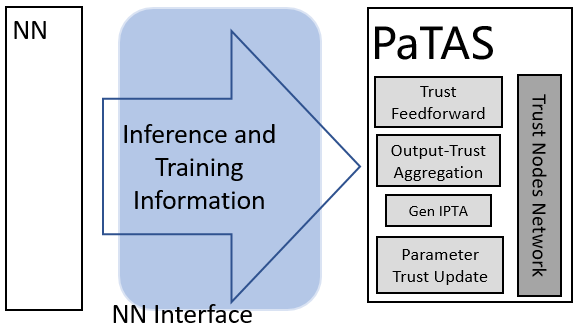
\includegraphics[width=0.5\linewidth]{img/patas/highPaTAS.png}
    \caption{High-Level Overview of the Trust Propagation in \ac{NN}}
    \label{fig:highptas}
\end{figure}

\begin{figure}
    \centering
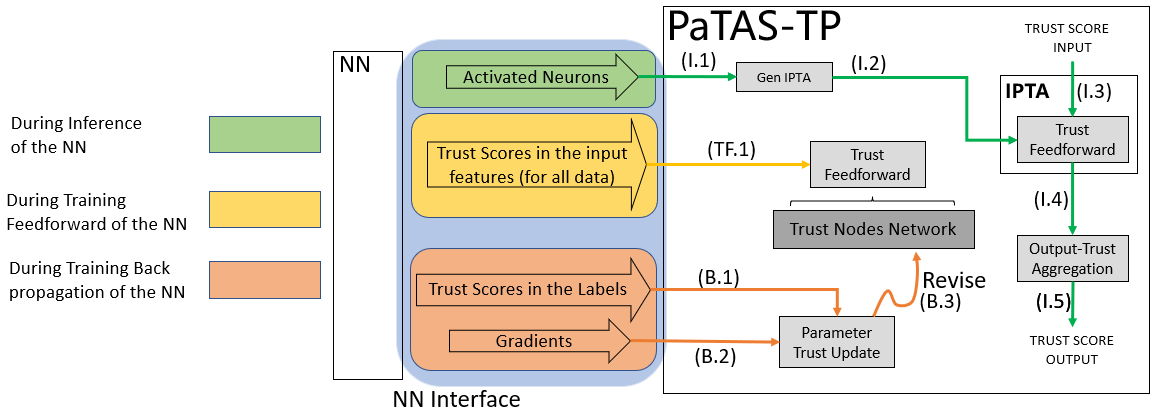
\includegraphics[width=0.8\textwidth]{img/patas/operations.png}

\caption{
    Functional flow of \ac{PaTAS-TP} integrated with a \ac{NN}, showing the interaction between the Trust Feedforward (TF), Parameter-Trust Update (B), and \ac{GenIPTA}/Output-Trust Aggregation (I) modules across the training and inference phases. \textbf{Feedforward (Training Phase):} The NN interface extracts trust scores from input features for all data being processed. These trust scores are passed to the \textit{Trust Feedforward} module (TF.1), which propagates them through the \textit{\ac{TNN}} in parallel with the \ac{NN} computations. During training, Trust Feedforward stores the trust scores of all intermediate computations in the NN, to be reused in backpropagation.    
    \textbf{Backpropagation (Training Phase):} Once the NN computes gradients, the trust scores of the labels (B.1) and the gradients (B.2) are provided to the \textit{Parameter-Trust Update}. Gradients indicate how dataset labels affect parameter updates, while label trust determines whether these updates should be considered reliable. The stored intermediate trust values are also incorporated in this process. Finally, the \textit{Parameter-Trust Update} module refines the trust values of the \ac{TNN} parameters (B.3), aligning them with the evolving learning dynamics. 
    \textbf{Inference Phase:} 
    During operation, contextual information such as the set of activated neurons is retrieved. This information is passed to \textit{\ac{GenIPTA}} (I.1), which constructs an \textit{\ac{IPTA}} corresponding to the specific inference path (I.2). The \ac{IPTA} takes input trust scores (I.3), propagates them along the path, and produces trust scores for each NN output. These can then be passed to the \textit{Output-Trust Aggregation} (I.4) which will combine them into a single consolidated trust score representing the reliability of the prediction (I.5).}
    \label{fig:ptasoperation}
\end{figure}

The backbone of \ac{PaTAS-TP} is the \emph{\acf{TNN}}, which mirrors the topology of the underlying \ac{NN} at the level of trust opinions. The \ac{TNN} is built from a single primitive: the \emph{Trust Node}, which is the trust-domain counterpart of a neuron.
\begin{definition}[Trust Node]
A \emph{Trust Node} is an abstract computational unit associated with a neuron in a \ac{NN}. It receives trust opinions on the neuron’s inputs and produces a trust opinion on the neuron’s output. The structure of a Trust Node mirrors that of its corresponding neuron, but its computation is defined over trust opinions.
\end{definition}
\noindent The parameters of the Trust Nodes are trust opinions rather than real-valued weights; they are initialized as vacuous opinions and refined during training by the Parameter-Trust Update module. The \ac{TNN} is a structured composition of Trust Nodes that mirrors the topology of the underlying \ac{NN}, propagating trust assessments layer by layer using the trust operations defined over each node. Each Trust Node receives trust opinions from its predecessors, applies its corresponding transformation, and passes the resulting opinion to its successors. 

The \ac{TNN} serves as the shared underlying representation for all four modules of \ac{PaTAS-TP}. 

\paragraph{Trust Feedforward}
The Trust Feedforward function propagates trust values through the \ac{TNN} in alignment with the \ac{NN}’s inference flow. It mirrors the layer-wise computations of the original model, but operates entirely on trust values. At each layer, trust in the inputs and parameters is combined using the trust operations, capturing how evidence flows through the network. This process produces a trust opinion for each output neuron of the \ac{NN} while also storing intermediate trust scores, which are later used by the Parameter-Trust Update.

\paragraph{Output-Trust Aggregation}
The Trust Feedforward function produces a vector of trust values, one for each output neuron. The goal of Output-Trust Aggregation is to combine these individual opinions into a single, consolidated trust score representing the overall trust in the network's output. This combination can be performed using a SL fusion operator, which fuses the trust opinions of all output Trust Nodes into one aggregated opinion. Alternatively, instead of aggregating across all outputs, one may directly consider the trust assigned to the final decision. For instance, in digit classification, if the model outputs a probability \(0.9\) for class ‘1’, the trust in the decision can be taken as the trust score associated with the output neuron for class ‘1’. More generally, the aggregation can be weighted by the strength of each output, for instance by the softmax probabilities, such that higher-confidence outputs contribute more heavily to the consolidated trust score. Finally, because every layer applies one round of discounting, aggregated trust decays geometrically with depth; a \emph{depth-normalized} variant therefore rescales the aggregated opinion by the inverse of this per-layer decay, making trust values comparable across architectures of different depths. Both the raw and the depth-normalized aggregate are used in the evaluation.

\paragraph{\acf{GenIPTA}}

The purpose of the \ac{GenIPTA} module is to dynamically construct a function tailored to a single, specific inference. This function, called \ac{IPTA}, reflects how trustworthy the exact computational path taken during that inference is. When an inference is performed, contextual information is recorded, such as the list of neurons activated along the path. In this case, the activation trace is used to instantiate a temporary subnetwork of Trust Nodes containing only the Trust Nodes corresponding to those activations, thereby mirroring the precise inference path of the \ac{NN}. Contextual information is not limited to activation traces. Typically, all neurons are activated to some degree, but only a subset of these activations is strongly relevant to the decision. \ac{GenIPTA} can therefore operate on truncated activation sets that retain only the most relevant neurons, which allows for more focused and interpretable trust assessments of the actual decision-making process. The \ac{GenIPTA} can also work in a more complex way by using the actual activation values of all neurons, performing a weighted trust assessment where stronger activations contribute more heavily to the trust inference.

\paragraph{Parameter-Trust Update}
The Parameter-Trust Update refines the trust opinions stored in the \ac{TNN} parameters during training, based on gradient information, input trust, and label trust to align parameter reliability with the evolving learning dynamics; its full formulation is presented in \cref{sec:param_update}.

The detailed functional flow of \ac{PaTAS-TP} across feedforward, backpropagation, and inference is illustrated in \cref{fig:ptasoperation}. 

With the architecture of \ac{PaTAS-TP} established, the following section introduces the perceptron as a minimal working example, providing concrete intuition for the operators mechanisms that underpin the Trust Feedforward computation before their generalization to deep architectures in \cref{sec:dnn_trust}.

\section{Trust Feedforward in a Simple Model: The Perceptron Case}
\label{sec:perceptron}

To illustrate the proposed trust propagation framework for the feedforward, we begin with the simple case of a single-layer perceptron. This setting provides an intuitive and tractable example that highlights the key mechanisms underlying the parallel trust function before extending them to deep \acp{NN}.

Consider a perceptron defined by a linear function:
\begin{equation}
    y' = \theta_1 s + \theta_2 \, n_r,
    \label{eq:smodel}
\end{equation}
\noindent where $s$ and $n_r$ denote input features (e.g., size and number of rooms in a apartment price estimation problem), and $\theta_1$, $\theta_2$ are the corresponding parameters.

We assume that trust assessments are available for:
\begin{itemize}
    \item the input features: $T_s$ and $T_{n_r}$,
    \item the parameters: $T_{\theta_1}$ and $T_{\theta_2}$.
\end{itemize}
\noindent The objective is to determine the resulting trust opinion $T(y')$ on the output, given these inputs.

\paragraph{Trust Propagation from Inputs}
\begin{figure}
\centering
\begin{subfigure}{0.44\linewidth}
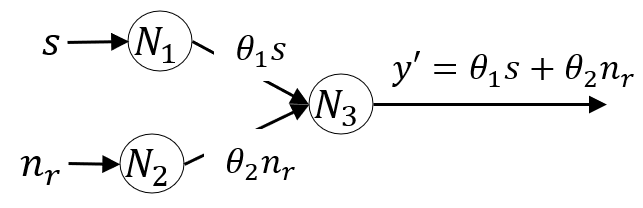
\includegraphics[width=\textwidth]{img/patas/NN1.png}
     \caption{Perceptron for \cref{eq:smodel}}
     \label{fig:nn1}
\end{subfigure}
\begin{subfigure}{0.55\linewidth}
    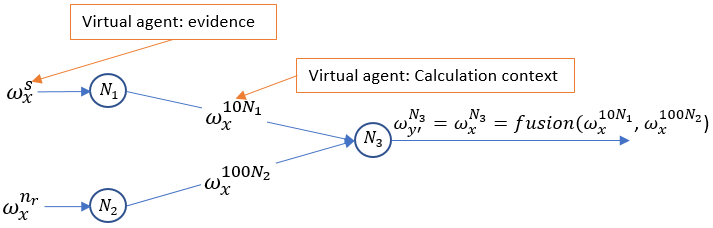
\includegraphics[width=\textwidth]{img/patas/NN1S.png}
    \caption{Parallel Trust Function for \cref{eq:smodel}}
   \label{fig:nn1s}
\end{subfigure}
\caption{Trust-propagation based solely on input-feature trust}
\label{fig:solution1}
\end{figure}

We first consider the simplified case where the parameters are assumed to be fully trusted. In this setting, the output is entirely determined by the input features, and trust propagation reduces to combining the trust opinions associated with each feature. The model specified in \cref{eq:smodel} is equivalent to the NN depicted in \cref{fig:nn1}. This network employs a linear transformation without an activation function. The input vector is:
$$ 
x = \begin{pmatrix}
    s \\
    n_r
\end{pmatrix}
$$ 
Let $\omega_x^s$ be the trust opinion on $x$ based on $s$ and  $\omega_x^{n_r}$ the trust opinion on $x$ based on $n_r$. Since the output neuron $N_3$ computes \cref{eq:smodel}, we associate this computation with two agents: $\theta_1 N_1$ from the context of computing \(\theta_1\cdot s\) and $\theta_2 N_2$ from the context of computing \(\theta_2\cdot n_r\). The trust opinion of the output neuron \(N_3\) on \(x\) is then: 
\(\omega_x^{N_3} = \mathit{fusion}(\omega_x^{\theta_1 N_1}, \omega_x^{\theta_2 N_2})\). 

The choice of the fusion operator (that we will later denote by \(\oplus\)) depends on the semantics of \(s\) and \(n_r\) (see \cref{sec:fusion}). In this two-feature example, $s$ and $n_r$ are independent measurements, so cumulative fusion, which accumulates the evidence of independent sources, would be semantically admissible. This independence does not survive the generalization to deep networks: from the second layer on, the opinions entering a neuron are computed from shared upstream inputs and parameters, and cumulative fusion would count the same evidence several times. \Cref{sec:fusion_choice} therefore instantiates $\oplus$ as an averaging fusion, and the perceptron example should be read with $\oplus$ as a generic fusion operator.

Assuming full trust in the parameters \(\theta_1\) and \(\theta_2\), we have:
\begin{align}
    \omega_x^{\theta_1 N_1} = \omega_x^{N_1} = \omega_x^{s} = T_s \, \text{ (Trust in the feature \(s\) of \(x\))} \notag \\
    \omega_x^{\theta_2 N_2} = \omega_x^{N_2} = \omega_x^{n_r} = T_{n_r} \, \text{ (Trust in the feature \(n_r\) of \(x\))} \notag 
\end{align}

Since the output value is deterministically related to the input via
\[
y' = f(x),
\]
the trust opinion of \(N_3\) on \(y'\) is the same as the trust opinion already computed for \(x\). Clearly, The transformation performed by \(f\) is encoded in the agent algebra, not in the variable algebra. Thus,
\begin{align}
    \omega_{y\prime}^{N_3} &= \omega_x^{N_3} = \omega_x^{\theta_1 N_1} \oplus \omega_x^{\theta_2 N_2} \notag \notag \\
&= \omega_x^{s} \oplus \omega_x^{n_r} = T_s \oplus T_{n_r}
\end{align}
In summary, if we define \(T_x = \begin{pmatrix}
    T_s&T_{n_r}
\end{pmatrix} \), then:
\[\pf_\Theta(T_x) = \pf_\Theta(\begin{pmatrix}
    T_s&T_{n_r}
\end{pmatrix}) =  T_s \oplus T_{n_r} \]
This formulation reflects the fact that the output trust aggregates evidence from multiple input sources, each contributing to the final prediction.

\paragraph{Incorporating Parameter Trust}
We now consider the general case where parameters are not assumed to be fully reliable. In this setting, parameter trust acts as a filtering mechanism that modulates the contribution of each input feature. Unlike the previous problem, where we fully trusted \(\theta_1\) and \(\theta_2\), here we do not fully trust these parameters, and we must account for their trust assessments. For the network to incorporate the trust in \(\theta_1\) and \(\theta_2\), we adjust the trust opinions on the features accordingly. The trust opinions are now refined.
\begin{figure}
    \centering
    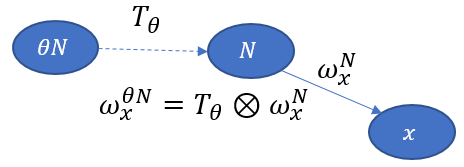
\includegraphics[width=0.4\linewidth]{img/patas/multprob2.png}
    \caption{Trust-propagation Trust Network with parameter trust.}
    \label{fig:multprob2l}
\end{figure}
As depicted in \cref{fig:multprob2l}, we model this as a small \aclu{STN}. therefore:
\begin{align}
    \omega_x^{\theta_1 N_1} = T_{\theta_1} \otimes \omega_x^{N_1} \; \text{and} \;
    \omega_x^{\theta_2 N_2} =  T_{\theta_2} \otimes \omega_x^{N_2}
\end{align}
where \(\otimes\) is a trust discounting operator. This results is consistent with the solution for problem 1 as for fully trusted \(T_\theta=(1,0,0)\), we have \(\omega_x^{\theta N} = T_{\theta} \otimes \omega_x^{N} = \omega_x^{N}\) (for any neuron \(N\)).

Finally, the resulting output trust \(\omega_{y\prime}^{N_3}\) is calculated by the fusion of these adjusted trust opinions: 
\begin{equation}
\label{eq:sol}
    \pf_\Theta(T_x) = \pf_\Theta(\begin{pmatrix}
    T_s&T_{n_r}
\end{pmatrix}) =  (T_{\theta_1}\otimes T_s)\oplus (T_{\theta_2}\otimes T_{n_r})
\end{equation}
Thus, we adjust the trust in the network output based on the trust in both the parameters and the features, ensuring that the trust propagation takes into account the trust in the parameters.

\paragraph*{Locality of the construction.} The \ac{STN} of \cref{fig:multprob2l} is local: it applies to a single neuron and models how the trust in one parameter modulates the trust contribution of one input. The trust computation of a whole network is obtained by applying this local rule neuron by neuron (\cref{sec:dnn_trust}), and each application only needs the incoming opinions of the neuron at hand. The construction therefore does not require the \ac{DSPG} property of \cref{chap:tnasl}. An alternative design that builds a single trust network across a path of neurons, with one edge per parameter and one node per intermediate activation, yields a graph that in general is not a \ac{DSPG} (\cref{fig:on_dspg_NN}); for such designs, and for the dataset trust assessment of \cref{chap:dataset-trust}, the \ac{DSPG} synthesis and analysis of \cref{chap:tnasl} remain the relevant tools.

This expression highlights two key mechanisms:
\begin{itemize}
    \item \textbf{Trust Discounting:} Parameter trust modulates the reliability of each input contribution.
    \item \textbf{Trust Fusion:} The resulting contributions are aggregated to form the final output trust.
\end{itemize}
\noindent The perceptron case reveals the fundamental principles of trust propagation in \acp{NN}. First, trust is \emph{compositional}: the output trust is constructed from the contributions of individual components. Second, trust is \emph{transformed}: parameter trust acts as a filter that attenuates or amplifies the influence of input trust. Third, trust is \emph{aggregated}: multiple sources of evidence are combined using fusion operators. 

In the next section, we generalize these principles to deep \acp{NN}, where trust must be propagated across multiple layers and intermediate activations.


\section{Generalization to Deep \acp{NN}}
\label{sec:dnn_trust}

The perceptron example introduced in the previous section highlights the fundamental mechanisms of trust propagation during feedforward. We now extend these principles to deep \acp{NN}, where trust must be propagated across multiple layers and intermediate representations. Consider a \ac{NN} ($\Theta$) composed of $L$ layers, where each layer defines a transformation:
\[
h^{(l)} = f^{(l)}\left(W^{(l)} h^{(l-1)} + b^{(l)}\right), \quad l = 1, \dots, L,
\]
with $h^{(0)} = x$ and $h^{(L)} = y'$.

In the trust domain, we associate a trust opinion $T^{(l)}$ to each layer output $h^{(l)}$, such that:
\[
T^{(l)} = T\left(h^{(l)}\right), \quad l = 0, \dots, L,
\]
In particular
\[
T^{(0)} = T\left(h^{(0)}\right) = T_x, \quad T^{(L)} = T\left(h^{(L)}\right) = T(y') = Pf_\Theta(T_x)\protect
\]
Trust propagation is then defined recursively as:
\[
T^{(l)} = f_T^{(l)}\left(T^{(l-1)}, T^{(l)}_{\Theta}\right),
\]
where $T^{(l)}_{\Theta}$ denotes the trust associated with the parameters of layer $l$, and $f_T^{(l)}$ is the trust transformation corresponding to the \ac{NN} operation at that layer. This formulation extends the parallel trust function introduced in \cref{sec:trust_foundations} to a layer-wise decomposition, where trust is propagated sequentially through the network in a manner consistent with the forward computation. In practice, as developed in the \ac{GenIPTA} module, the parallel function is not defined once for the whole network but instantiated per inference, since the active computational path depends on the specific input. 

To formalize this process, we introduce the concept of trust function.
\begin{definition}[Trust Function]\label{def:trustfunc}
A \emph{Trust Function} models the transformation of trust through a Trust Node. It defines how trust opinions on the inputs of a neuron are combined to produce a trust opinion on the output. 
For a neuron that computes
\(
z^{(l)} = \sum \theta^{(l)}_i \cdot x^{(l)}_i, \quad x^{(l+1)} = \phi^{(l)}(z^{(l)}),
\)
the corresponding trust computation is given by:
\[
T_{z^{(l)}} = \bigoplus_{i=1}^{d} T_{x_{i}^{(l)}} \otimes T_{\theta_{i}^{(l)}}, \quad
T_{x^{(l+1)}} = T_{\phi^{(l)}}(T_{z^{(l)}}),
\]
\begin{itemize}
    \item \( \otimes \) is a trust discounting operator,
    \item \(\bigoplus\) is a trust fusion operator,
    \item \( T_{\phi}^{(l)} \) is the trust-equivalent of the activation function. In this work, we set it to identity function as we use ReLU as activation function.
\end{itemize}
\end{definition}

\paragraph*{Instantiation of the operators.} Throughout this thesis, $\otimes$ is the probability-sensitive trust discounting operator of \ac{SL}~\cite{josang2016subjective}: with $P_\theta = b_\theta + a\,u_\theta$ the projected probability of the parameter opinion,
\(
T_\theta \otimes T_x = \big(P_\theta\, b_x,\; P_\theta\, d_x,\; 1 - P_\theta (b_x + d_x)\big).
\)
The fusion $\bigoplus$ over the $d$ contributions entering a neuron is instantiated as an \emph{averaging} fusion: the fused opinion is the component-wise mean of the discounted opinions,
\[
\bigoplus_{i=1}^{d} \omega_i = \Big(\tfrac{1}{d}\textstyle\sum_i b_i,\; \tfrac{1}{d}\sum_i d_i,\; \tfrac{1}{d}\sum_i u_i\Big).
\]
This is the multi-source averaging belief fusion of van der Heijden et al.~\cite{vanderheijden2018multisourcefusionoperationssubjective} for sources of equal uncertainty; when the uncertainties differ, the general operator additionally weights every source by the product of the uncertainties of the other sources, whereas the implementation keeps equal weights, so that a layer reduces to a matrix product over projected probabilities and scales to wide layers. Both forms share the properties that matter here. They fuse all incoming opinions of a neuron at once, so the result does not depend on a pairwise grouping (averaging fusion is not associative). They are idempotent, so an opinion that reaches a neuron several times does not inflate the evidence. And they preserve zero belief and zero disbelief: if no input carries disbelief, the fused opinion carries none. Cumulative fusion, which the perceptron example of \cref{sec:perceptron} motivates for independent measurements, is deliberately not used; \cref{sec:fusion_choice} explains why.

\paragraph*{Expressiveness limits.} Two restrictions of the trust functions should be stated before they are used, because they bound what the propagated opinions can express. First, the trust functions see only the opinions attached to the quantities entering a computation, not the quantities themselves: the sign and magnitude of a weight and the value of an activation do not enter \cref{def:trustfunc}, and the trust counterpart of the ReLU activation is the identity. An input that the network effectively ignores therefore contributes to the output opinion exactly as an input that dominates the decision, unless the inference path is restricted to the active neurons, as the \ac{IPTA} does (\cref{sec:tp_arch_ovvw}), or weighted by activity (\cref{sec:conv_trust}). Second, discounting scales belief and disbelief by the same factor $P_\theta$ and moves the remainder to uncertainty, and averaging fusion cannot create disbelief from opinions that carry none. Output disbelief can therefore only originate from disbelief in the input: untrustworthy parameters manifest as output uncertainty, never as output disbelief (\cref{thm:infvac} and \cref{rem:directional}). In particular, every experiment of \cref{sec:patas-tp-evaluation} that feeds a fully trusted input obtains $d = 0$ at the output by construction, and the informative quantity in those experiments is the split of the remaining mass between belief and uncertainty.

\begin{figure}[htbp]
\centering
\begin{subfigure}{0.2\textwidth}   
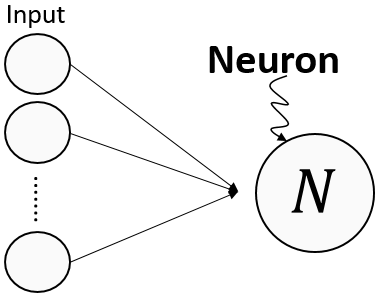
\includegraphics[width=\textwidth]{img/patas/trust_node/neuron.png}
  \caption{Structure of a Perceptron}
  \label{fig:neuron}
\end{subfigure}
\begin{subfigure}{0.2\textwidth}
  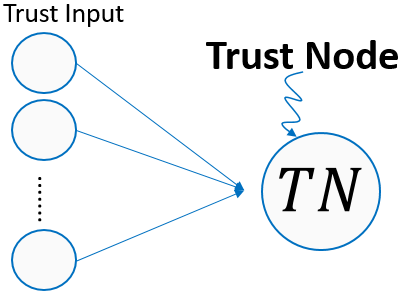
\includegraphics[width=\textwidth]{img/patas/trust_node/trustnode.png}
  \caption{Mirrored Trust Structure}
  \label{fig:tns}
\end{subfigure}

\begin{subfigure}{0.45\textwidth}
  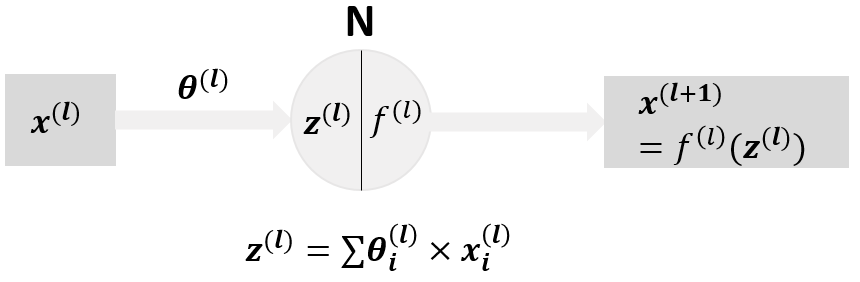
\includegraphics[width=\textwidth]{img/patas/trust_node/neurop.png}
  \caption{Perceptron Operation}
  \label{fig:neuronfunc}
\end{subfigure}
\begin{subfigure}{0.45\textwidth}
  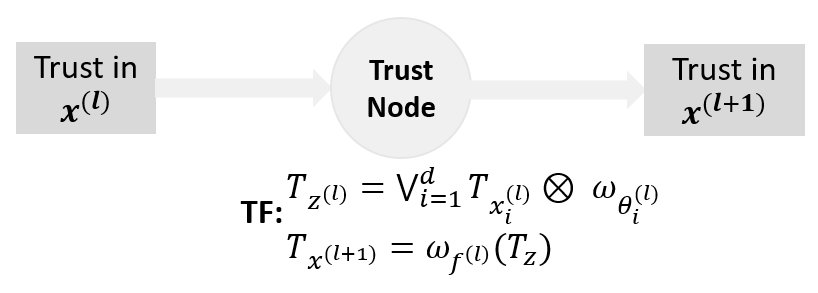
\includegraphics[width=\textwidth]{img/patas/trust_node/tnop.png}
  \caption{Trust Function Operation}
  \label{fig:tnf}
\end{subfigure}

\caption{Illustration of the Trust Node structure and computation}
\label{fig:trustnode}
\end{figure}

% In particular, the two fundamental operations identified in the perceptron case generalize as follows:
% \begin{itemize}
%     \item \textbf{Weighted Contributions (Discounting):} The influence of an input activation on a neuron is modulated by the trust in the corresponding weight. This is modeled using the trust discounting operator:
%     \[
%     T_{\text{contrib}} = T_{\theta} \otimes T_{\text{input}}.
%     \]
    
%     \item \textbf{Aggregation (Fusion):} Multiple contributions to a neuron are combined using a fusion operator:
%     \[
%     T_{\text{node}} = \bigoplus_i T_{\text{contrib}, i}.
%     \]
% \end{itemize}
% Activation functions can be interpreted as transformations that preserve or reshape trust without introducing new sources of evidence. In this work, we assume that activation functions do not alter the trust opinion directly, but only affect the structure of the propagation by activating or deactivating certain paths.

\Cref{fig:trustnode} illustrates the structural correspondence between a standard neuron and its associated Trust Node. \cref{fig:neuron,fig:tns} show how the mirrored trust structure is derived from the original perceptron, while \cref{fig:neuronfunc,fig:tnf} contrast the numerical computation of the neuron with the trust-domain computation of the Trust Function, in which multiplication is replaced by discounting and summation by fusion. 

% Combining these elements, trust propagation in a deep \ac{NN} proceeds as follows:
% \begin{enumerate}
%     \item \textbf{Initialization:} Assign trust opinions $T^{(0)} = T(x)$ to the input features.
    
%     \item \textbf{Layer-wise Propagation:} For each layer $l = 1, \dots, L$:
%     \begin{itemize}
%         \item Compute discounted contributions from the previous layer using parameter trust.
%         \item Aggregate contributions using a fusion operator.
%         \item Assign the resulting trust to the current layer: $T^{(l)}$.
%     \end{itemize}
    
%     \item \textbf{Output Trust:} The final trust opinion is given by $T(y') = T^{(L)}$.
% \end{enumerate}

\begin{algorithm}
\caption{Trust Feedforward}
\begin{algorithmic}[1]
\Require Input trust $T^{(0)} = T(x)$, parameter trust 
         $\{T^{(l)}_\Theta\}_{l=1}^{L}$
\Ensure Output trust $T(y') = T^{(L)}$

\For{each layer $l = 1, \dots, L$}
    \For{each neuron $i$ in layer $l$}
        \State Compute discounted contributions:
        \[
        T_{\text{contrib},j} = T_{\theta^{(l)}_{i,j}} \otimes T^{(l-1)}_{x_j}, 
        \quad \forall j \in \mathcal{N}(i)
        \]
        
        \State Aggregate contributions via fusion:
        \[
        T_{z^{(l)}_i} = \bigoplus_{j \in \mathcal{N}(i)} T_{\text{contrib},j}
        \]
        \State Apply activation trust:
        \[
        T^{(l)}_{x_i} = T_{\phi^{(l)}}(T_{z^{(l)}_i})
        \]
    \EndFor
\EndFor
\State \Return $T(y') = T^{(L)}$
\end{algorithmic}
\label{alg:trustff}
\end{algorithm}

\subsection{Dependence between Fused Opinions and the Choice of the Fusion Operator}
\label{sec:fusion_choice}
The fusion step of \cref{def:trustfunc} combines the discounted contributions $T_{\theta_i} \otimes T_{x_i}$ that enter a neuron. In the perceptron of \cref{sec:perceptron}, these contributions come from distinct input features and can be treated as independent evidence. The first layer is the only place where this assumption can hold. From the second layer on, all incoming opinions of a neuron are computed from the same set of upstream inputs and parameters, so the same evidence reaches the neuron through several paths, and a fusion operator that accumulates evidence counts it several times. Under cumulative fusion the output uncertainty would shrink with the width of the network alone: with two inputs carrying the opinion $(0.5, 0, 0.5)$, fully trusted parameters, no bias terms and one hidden layer of width $n$, the output opinion is $(0.8, 0, 0.2)$ for $n = 2$ and $(0.996, 0, 0.004)$ for $n = 128$, although no evidence has been added. The averaging fusion adopted above returns $(0.5, 0, 0.5)$ for every $n$: duplicated opinions do not inflate the evidence, and the operator is an equal-weight simplification of the one \ac{SL} prescribes for dependent sources (\cref{sec:fusion}).

Averaging fusion removes the double counting of identical opinions, but it does not model the correlation between opinions that are dependent without being identical, and nested averaging across layers weights an input by the number of paths through which it reaches the output rather than treating it as one source. Consider an input $x_1$ with opinion $(0.5, 0, 0.5)$ that feeds two hidden neurons and a vacuous input $x_2$ that feeds only one of them, a situation that arises after \ac{IPTA} pruning. With fully trusted parameters and no bias terms, the output opinion is $(0.375, 0, 0.625)$, whereas averaging $x_1$ and $x_2$ directly as two sources gives $(0.25, 0, 0.75)$. The propagated opinion is thus a path-weighted rather than a source-weighted aggregate. This is a limitation of the design that the experiments of \cref{sec:patas-tp-evaluation} do not remove, and it is one reason why absolute trust values are only comparable within one architecture, as discussed in \cref{sec:patas-discussion}. The same argument applies to residual connections (\cref{sec:conv_trust}): the input and output opinions of a residual block are not independent, the output being computed from the input, so a skip connection is mapped to averaging rather than cumulative fusion.

Because the local rule of \cref{def:trustfunc} is applied neuron by neuron, the properties established in \cref{sec:ptassyminv} use only properties of the operators themselves, namely the discounting of a vacuous opinion, the symmetry of discounting and fusion in belief and disbelief, and the preservation of zero belief or zero disbelief under fusion. They therefore hold for any architecture to which the rule is applied, independently of the graph structure.

\subsection{Extension to Convolutional Architectures}
\label{sec:conv_trust}
The construction above is stated for fully connected layers, but nothing in it is specific to them; what changes in a \ac{CNN} is weight sharing. \ac{PaTAS-TP} mirrors a convolutional layer with $c_{\mathrm{in}}$ input channels, $c_{\mathrm{out}}$ output channels, and kernel size $k$ by one opinion matrix of shape $(c_{\mathrm{in}} k^2 + 1) \times c_{\mathrm{out}}$, exactly the flattened kernel matrix that also carries the layer's gradients, so the Parameter-Trust Update of \cref{sec:param_update} applies unchanged. For the feedforward, the input pixel opinions are fused into per-channel opinions and the layer is applied as the standard dense discount-fusion rule on the flattened kernel matrix; this \emph{uniform-trust reduction} is exact whenever the input trust is spatially uniform (the trusted, vacuous, and distrusted profiles used throughout) and an approximation otherwise. ReLU and pooling remain identity in opinion space, and a residual skip connection is mapped to averaging fusion of the block's input and output opinions: the two opinions are dependent, the output of the block being computed from its input, so cumulative fusion would count the input's evidence twice (\cref{sec:fusion_choice}).

The \ac{IPTA} generalizes as well, with one conceptual change. In a fully connected network an inference path selects \emph{weights}: inactive neurons remove their rows from the trust computation. Under weight sharing a path cannot select weights, only \emph{applications} of a filter, since the same kernel is applied at every spatial position. The convolutional \ac{IPTA} therefore weights each channel's contribution by its \emph{participation degree}: the fraction of spatial positions at which the channel's post-ReLU output is positive for the given input. Formally, the discount-fusion step becomes a weighted fusion in which row $j$ of the opinion matrix enters with weight $w_j$ equal to the producing channel's participation (bias rows keep weight $1$). For binary participation this reduces \emph{exactly} to the row-pruned computation of the fully connected \ac{IPTA}, so the convolutional variant is a strict generalization: channels the forward pass never activated contribute nothing, and partially active channels contribute in proportion to their actual involvement in the decision.

\Cref{alg:trustff} formalizes this layer-wise computation as the complete Trust Feedforward pipeline. This generalization demonstrates that trust propagation can be integrated into deep \acp{NN} without altering their structure, by defining a parallel computation over trust opinions. It makes the link between output trust $T_{y'}$, input trust $T_{x}$, and parameter trust $T_{\theta}$: 
\[T_{x} \xrightarrow{T_\theta} T_{y'}.\] In the next section, we focus on how parameter trust is computed during training, completing the link between dataset trust and model trustworthiness:
\[T_{\dataset} \rightarrow T_\theta.\] 

\section{Parameter-Trust Update}\label{sec:param_update}
The Parameter-Trust Update is the mechanism through which \ac{PaTAS-TP} adapts the trust associated with model parameters during training. Its objective is to ensure that parameter trust reflects both the observed behavior of the model and the reliability of the training data. Its design is inspired by the standard backpropagation algorithm used in \ac{NN} training, where gradients quantify how much each parameter contributes to the output error. By leveraging these gradients as evidence, \ac{PaTAS-TP} updates parameter trust in a way that mirrors the learning dynamics of the underlying model.

To ground the design, we briefly recall the standard parameter update in \ac{NN} training. For a parameter $\theta$, gradient descent updates are given by:
\begin{equation}
\label{eq:gd1}
\theta \leftarrow \theta - l_r  \frac{\partial \mathcal{L}}{\partial \theta},
\end{equation}
where $l_r$ is the learning rate, $\mathcal{L}$ is the loss function, and $\frac{\partial \mathcal{L}}{\partial \theta}$ is the gradient. These gradients are computed recursively using the chain rule:
\begin{equation}
\label{eq:gd2}
\frac{\partial \mathcal{L}}{\partial \theta^{(l)}_{i,j}}
= \delta^{(l)}_i x^{(l-1)}_j,
\end{equation}
where $\theta^{(l)}_{i,j}$ denotes the weight connecting neuron $j$ in layer $(l-1)$ to neuron $i$ in layer $l$, $\delta^{(l)}_i$ is the error term of neuron $i$, and $x^{(l-1)}_j$ is the activation from the previous layer.

In particular, \cref{eq:gd2} shows that gradients factor into an error term and an input activation, revealing that parameter updates depend jointly on gradient signals, input activations, and learning dynamics. \ac{PaTAS-TP} mirrors this structure by incorporating gradient information, input trust, and label trust as analogous sources of evidence in the Parameter-Trust Update. At a high level, the parameter-trust update process combines three sources of information: (i) gradient-based evidence derived from backpropagation, (ii) trust in the labels within the current training batch, and (iii) trust in the input features and intermediate computations recorded during feedforward. These elements are integrated to revise and refine the trust assigned to each parameter. The notation used throughout this subsection is summarized in \cref{tab:symbols}, and the complete update procedure is given in \cref{alg:trustupdate}.

\begin{algorithm}
\caption{Parameter-Trust Update Algorithm}
\begin{algorithmic}[1]

    \Function{ParameterTrustUpdate}{$g, T_y, T_{lr}, \epsilon$}
        \Statex \hspace{\algorithmicindent}\textbf{Summary:} Revises and updates the trust parameters of the Trust Nodes by combining gradient evidence, label trust, and neuron input trust, under mini-batch training.
        \Statex \hspace{\algorithmicindent}\textbf{Step 1:} Compute the batch label opinion (component-wise mean over the batch)
        \State $T_{y_\text{batch}}  \longleftarrow  \frac{1}{|y_\text{batch}|}\sum_{y \in y_\text{batch}} T_y$ \label{alg:l:ybatch}
        \For{each layer $l$}
            \For{each neuron $n_i^{(l)}$}
                \Statex \hspace{3\dimexpr\algorithmicindent\relax}\textbf{Step 2:} Gather gradient $g$ for neuron $n_i^{(l)}$
                \State $g^{(l)}_i  \longleftarrow  \{\, g^{(l)}_{i,j} \;|\; j \in \mathcal{N}(i)\,\}$ \label{alg:l:grad}
                \Statex \hspace{3\dimexpr\algorithmicindent\relax}\textbf{Step 3:} Compute trust for neuron $n_i^{(l)}$
                \State $T_{n_i \mid y_\text{batch}}  \longleftarrow $ \Call{NodeTrust}{$g^{(l)}_i, T_{y_\text{batch}}, \epsilon$} \label{alg:l:nodetrust}
                \Statex \hspace{3\dimexpr\algorithmicindent\relax}\textbf{Step 4:} Deduce overall trust in neuron $n_i^{(l)}$
                \State $T_{n_i \parallel Y_\text{batch}}  \longleftarrow $ \Call{DeduceTrust}{$T_{n_i \mid y_\text{batch}}, T_{n_i \mid \lnot y_\text{batch}}, T_{y_\text{batch}}$} \label{alg:l:deduce}
                \For{each incoming edge $j$ to $n_i^{(l)}$}
                    \Statex \hspace{4\dimexpr\algorithmicindent\relax}\textbf{Step 5:} Revise parameter trust with node trust
                    \State $T_{\theta_{i,j}^{(l)}}  \longleftarrow $ \Call{Revise}{$T_{\theta_{i,j}^{(l)}}, T_{n_i \parallel Y_\text{batch}}$} \label{alg:l:revise}
                    \Statex \hspace{4\dimexpr\algorithmicindent\relax}\textbf{Step 6:} Update parameter trust with auxiliary factors
                    \State $T_{\theta_{i,j}^{(l)}} \longleftarrow $ \Call{Update}{$T_{\theta_{i,j}^{(l)}}, T_{x^{(l-1)}_j}, T_{y_\text{batch}}, T_{lr}$} \label{alg:l:update}
                \EndFor
            \EndFor
        \EndFor
    \EndFunction

    \Function{NodeTrust}{$g^{(l)}_i, T_{y_\text{batch}}, \epsilon$}
        \State Count $r$: \#edges with $|g^{(l)}_{i,j}| < \epsilon$
        \State Count $s$: \#edges with $|g^{(l)}_{i,j}| \geq \epsilon$
        \State Map $(r,s)$ into a binomial opinion using Baseline-Prior Quantification
        \State \Return $T_{n_i \mid y_\text{batch}}$
    \EndFunction

    \Function{DeduceTrust}{$T_{n_i \mid y_\text{batch}}, T_{n_i \mid \lnot y_\text{batch}}, T_{y_\text{batch}}$}
        \State $T_{n_i \mid \lnot y_\text{batch}}  \longleftarrow  (0,0,1)$
        \State \Return $T_{n_i \parallel Y_\text{batch}} = T_{y_\text{batch}} \circledcirc (T_{n_i \mid y_\text{batch}}, T_{n_i \mid \lnot y_\text{batch}})$
    \EndFunction

    \Function{Revise}{$T_{\theta_{i,j}^{(l)}}, T_{n_i \parallel Y_\text{batch}}$}
        \State \Return $T_{\theta_{i,j}^{(l)}} \circleddash T_{n_i \parallel Y_\text{batch}}$ \Comment{$\circleddash$ instantiated as averaging fusion}
    \EndFunction

    \Function{Update}{$T_{\theta}, T_{x}, T_{y_\text{batch}}, T_{lr}$}
        \State $T_{\theta} \longleftarrow T_{\theta} \circleddash (T_{\theta} \odot T_{lr})$ \Comment{learning-rate adjustment} \label{alg:l:lr}
        \State \Return $T_{\theta} \odot (T_{x} \oslash T_{y_\text{batch}})$ \label{alg:l:aux}
    \EndFunction

\end{algorithmic}
\label{alg:trustupdate}
\end{algorithm}
The procedure described in \cref{alg:trustupdate} operates at the level of mini-batches and iterates over all layers and neurons of the network. For each neuron, it first derives a trust assessment based on gradient evidence and the reliability of the training labels, and then propagates this information to update the trust associated with its incoming parameters. More specifically, the update process can be decomposed into three main stages: (i) aggregation of label trust at the batch level, (ii) estimation of neuron-level trust using gradient information, and (iii) revision and adjustment of parameter trust using both inferred neuron trust and auxiliary factors such as input trust. We now describe these steps in detail.

The algorithm runs once per batch and begins by computing a single label opinion for the batch (Line~\ref{alg:l:ybatch}):
\(
T_{y_\text{batch}} = \frac{1}{|y_\text{batch}|}\sum_{y \in y_\text{batch}} T_y ,
\)
the component-wise mean of the label opinions of the batch, computed separately for each output class in the output layer. This is the averaging fusion of \cref{sec:fusion_choice} applied to the label opinions, and it serves as the conditioning opinion for every parameter update of the batch. A conjunction of the label opinions, which would express that \emph{all} labels of the batch are correct, is not appropriate here: the projected probability is multiplicative under \ac{SL} multiplication, so a batch of 64 labels with projected probability $0.95$ each would receive a batch opinion with projected probability $0.95^{64} \approx 0.04$, and the batch opinion would measure the batch size rather than the label quality. The mean opinion is idempotent, so a batch of identical label opinions carries that label opinion unchanged, and its expectation does not depend on the batch size. The remaining dependence of the parameter trust on the batch size enters through the gradient evidence and is quantified in \cref{sec:patas-tp-evaluation}.

For each neuron \(n_i^{(l)}\) at index \(i\) in layer \(l\), we compute:
\begin{itemize}
    \item \( T_{n_{i}^{(l)} \mid y_\text{batch}} \) (Line~\ref{alg:l:nodetrust}), the trust conditioned on the current batch labels. This is inferred by checking each incoming weight gradient \( g^{(l)}_{i,j} \): if \( |g^{(l)}_{i,j}| < \epsilon\)\footnote{The threshold $\epsilon$ is used only in the \textsc{NodeTrust} function, to separate weak from strong gradients. It is a sensitivity parameter that has to be set relative to the gradient scale of the task: Experiment~1 compares four values and retains $\epsilon = 0.1$ for the breast-cancer task, the MNIST experiments use $\epsilon = 0.05$, and the scale-tied rule introduced below removes the choice altogether.}
 it is counted as positive evidence \( r \), otherwise as negative evidence \( s \). These counts are then mapped into a binomial opinion using the Baseline-Prior Quantification model with prior weight $W = 2$, so that the uncertainty of this opinion, $u = W / (|\mathcal{N}(i)| + W)$, depends only on the number of incoming edges of the neuron.
    \item \( T_{n_{i}^{(l)} \mid \lnot y_\text{batch}} \), the trust when the true batch labels are not \( y_\text{batch} \). Since no concrete evidence is available for this case, it is initialized to a vacuous opinion: \( (0, 0, 1) \).
    \item A deduced trust \( T_{n_{i}^{(l)} \parallel Y_\text{batch}} \) (Line~\ref{alg:l:deduce}) using the inferential deduction operator \( \circledcirc \), combining the two conditional opinions with \( T_{y_\text{batch}} \).
\end{itemize}

Then for each incoming edge \( j\) of neuron \( i \), the parameter trust \( T_{\theta_{i,j}^{(l)}} \) is updated in two stages:
\begin{enumerate}
    \item Revision with the deduced trust (Line~\ref{alg:l:revise}), using the trust-revision operator $\circleddash$ of \cref{tab:symbols}:
    \[
    T_{\theta_{i,j}^{(l)}} \leftarrow T_{\theta_{i,j}^{(l)}} \circleddash T_{n_{i}^{(l)} \parallel Y_\text{batch}} .
    \]
    Throughout this thesis $\circleddash$ is instantiated as the two-source averaging belief fusion $\underline{\oplus}$ (\cref{sec:fusion}); the consequences of this choice, and of the alternatives, are analysed in \cref{sec:ptas_convergence}.
    \item Adjustment with auxiliary factors (Line~\ref{alg:l:update}):
    During training, the update of parameter $\theta_{i,j}^{(l)}$ depends not only on its current value but also on auxiliary factors such as the input $x^{(l-1)}_{j}$, the label $y_\text{batch}$ and the learning rate (see \cref{eq:gd1,eq:gd2}).
To reflect this, the parameter trust is first adjusted with the learning-rate opinion $T_{lr}$ (Line~\ref{alg:l:lr}),
\[
    T_{\theta_{i,j}^{(l)}} \longleftarrow T_{\theta_{i,j}^{(l)}} \circleddash \big(T_{\theta_{i,j}^{(l)}} \odot T_{lr}\big),
\]
and then with the input and label opinions (Line~\ref{alg:l:aux}):
\[
    T_{\theta_{i,j}^{(l)}} \longleftarrow T_{\theta_{i,j}^{(l)}} \odot (T_{x_j^{(l-1)}} \oslash T_{y_\text{batch}}).
\]
Here, $\odot$ is the binomial multiplication operator, evaluated with the base rate $a = 1/2$ used throughout this chapter, and $\oslash$ is defined as:
\begin{align}
    (b,d,u) &= (b_1, d_1, u_1) \oslash (b_2, d_2, u_2), \\
    b &= \min(b_1, b_2), \notag \\
    d &= \max(d_1, d_2), \notag \\
    u &= 1 - (b+d). \notag
\end{align}
This formulation reflects the fact that both unreliable features and mislabeled data can strongly bias parameter updates. The use of min and max provides a conservative aggregation: trust cannot exceed the weakest evidence, and distrust must reflect the strongest warning. It ensures that trust in both input features and labels is explicitly propagated into the parameter trust. In all experiments of this chapter the learning-rate opinion is fully trusted, $T_{lr} = (1,0,0)$. With base rate $1/2$, multiplication by a dogmatic opinion is not the identity: $(b,d,u) \odot (1,0,0) = (b + u/3,\; d,\; 2u/3)$ moves one third of the uncertainty mass to belief, and $(b,d,u) \odot (0,0,1) = (b/3,\; d,\; 1 - b/3 - d)$ moves two thirds of the belief mass to uncertainty. The two multiplication sub-steps therefore contract the parameter uncertainty at every batch under trusted data and expand it under vacuous data; \cref{sec:ptas_convergence} shows how this interacts with the averaging revision.
\end{enumerate}

\paragraph*{Scale-Tied Threshold.}
The threshold $\epsilon$ used by \textsc{NodeTrust} separates weak from strong gradients, and its natural scale is that of the gradients themselves, which varies across tasks and across layers. Rather than treating $\epsilon$ as an absolute constant, we therefore also define a \emph{scale-tied} variant: for each layer, $\epsilon_{\mathrm{layer}} = c \cdot \mathrm{median}(|\delta|)$, where the median gradient magnitude is estimated over the first revision batches of that layer and then frozen, and $c$ is a single dimensionless constant ($c = 0.5$ unless stated otherwise). This makes the stability criterion relative to the task's own gradient scale: the same rule instantiates thresholds differing by nearly two orders of magnitude across the tasks studied here without any per-task tuning. Its empirical validation is reported in \cref{sec:patas-discussion}.


\paragraph*{Computational Overhead during \ac{NN} training.}
The proposed \ac{PaTAS-TP} operates in parallel with the primary \ac{NN} and mirrors its computational flow using subjective opinions. When the two computations run on separate hardware and exchange gradients asynchronously, the execution time cost is bounded by
\[
\mathcal{C}_{\text{with \ac{PaTAS-TP}}} \approx \mathcal{C}_{\text{comm}} + \max(\mathcal{C}_{\text{PaTAS-TP}}, \mathcal{C}_{\text{NN}}),
\]
where \(\mathcal{C}_{\text{comm}}\) denotes the communication overhead between the \ac{NN} and the \ac{PaTAS-TP}. Each \ac{PaTAS-TP} operation is performed over subjective opinions represented by three stored components (belief, disbelief, uncertainty; the base rate is a shared constant), giving an analytical estimate of roughly \(\mathcal{C}_{\text{PaTAS-TP}} \approx 3 \times \mathcal{C}_{\text{NN}}\) for the propagation arithmetic and a threefold memory overhead for the opinion parameters. Measured costs on an A100 GPU (784-512-10 architecture) are consistent with this estimate at inference time: trust propagation costs $0.43$\,ms per batch, amortizing from $14.8\times$ overhead at batch size 1 to $3.7\times$ at batch size 512. The prototype used in this chapter does not realise the parallel bound during training: the \ac{NN} and \ac{PaTAS-TP} are synchronised batch by batch through a socket, so the training loop advances at the pace of the slower side, roughly $7$ optimization steps per second with \ac{PaTAS-TP} attached against $2200$ unattached for the same architecture on the same GPU. This is an engineering bottleneck of the socket-based prototype rather than of the method, and it affects wall-clock time only: training never consumes a value produced by \ac{PaTAS-TP}, so the learned parameters are identical with and without it. The training results of this chapter were obtained with \ac{PaTAS-TP} attached to the training loop in this synchronous mode, the revision consuming the gradient stream of the run; when several \ac{PaTAS-TP} configurations were compared for one trained model, the prototype regenerated the gradient stream by re-running the training loop from the cached model, and the replications reported in \cref{sec:patas-tp-evaluation} avoid this shortcut by attaching \ac{PaTAS-TP} to a fresh training run for every configuration. Since the revision does not feed back into training, it could equally be computed after training from a recorded gradient stream, which is the deployment mode described by the parallel bound above. The parallel design thus ensures that trust propagation does not interfere with the execution of the primary model, making the approach suitable for monitoring scenarios where interpretability and reliability are critical.



\section{Theoretical Properties of \ac{PaTAS-TP}}\label{sec:ptastheory}
To ensure that \ac{PaTAS-TP} provides reliable and interpretable trust assessments, we first establish several fundamental theoretical properties describing its stability and consistency.
\subsection{Stability of the Parameter-Trust Update}
\label{sec:ptas_convergence}

The stability of \ac{PaTAS-TP} is governed by the stability of its inputs and by the structure of its recursive Parameter-Trust Update. During training, \ac{PaTAS-TP} updates the internal trust opinions associated with network parameters using trust opinions on the inputs, labels and learning rate, and gradient information, as outlined in \cref{alg:trustupdate}. The update is a composition of three maps applied once per batch: the revision $T_\theta \circleddash q_n$ with the deduced node opinion $q_n = T_{n_i \parallel Y_\text{batch}}$, the learning-rate adjustment $T_\theta \circleddash (T_\theta \odot T_{lr})$, and the auxiliary adjustment $T_\theta \odot (T_x \oslash T_{y_\text{batch}})$. Two facts shape its behaviour. First, the node opinion $q_n$ is computed from thresholded mini-batch gradients, so its belief and disbelief change from batch to batch even after the network has converged, because stochastic gradient descent does not make the gradients constant; only its uncertainty $u_q = W / (|\mathcal{N}(i)| + W)$ is the same at every step. Second, none of the \ac{SL} fusion operators forms a group with the set of opinions: cumulative and belief constraint fusion have the vacuous opinion as identity but no inverses, since evidence cannot be negative; averaging fusion has no identity and is not associative; weighted fusion is not associative; and averaging and weighted fusion are idempotent, which in a group only the identity can be. The behaviour of the revision therefore has to be established operator by operator rather than from group structure, and the limit, when it exists, is not the same for all operators.

\begin{theorem}[Stability of the Parameter-Trust Update\footnote{All proofs of the theorems in this section are provided in the \appp (\cref{app:proof}).}]\label{thm:convergence}
Let $T_\theta^{(n)} = (b^{(n)}, d^{(n)}, u^{(n)})$ denote the opinion on a parameter $\theta$ after $n$ applications of \cref{alg:trustupdate} with base rate $a = 1/2$ and learning-rate opinion $T_{lr} = (1,0,0)$, and let $q_n$ be the node opinion fused at step $n$, with constant uncertainty $u_q$.
\begin{enumerate}
    \item \emph{Constant evidence, revision only.} If $q_n = q$ for all $n$ and the two adjustment sub-steps are omitted, the sequence $\omega_{n+1} = \omega_n \circleddash q$ converges, with a limit that depends on the operator. For a non-vacuous $q$: to $q$ under averaging and weighted fusion, geometrically; to the dogmatic opinion $(b_q, d_q, 0)/(b_q + d_q)$ under cumulative fusion, the uncertainty decaying like $1/n$; and, under belief constraint fusion, to the vertex $(1,0,0)$ if $b_q > d_q$, to $(0,1,0)$ if $d_q > b_q$, and to a dogmatic opinion whose ratio is fixed by $\omega_0$ if $b_q = d_q$. For a vacuous $q$, averaging fusion drives the sequence to the vacuous opinion, while cumulative, weighted and belief constraint fusion leave $\omega_0$ unchanged (\cref{thm:abf,thm:cbf,thm:bcf}).
    \item \emph{Implemented update, trusted data.} With averaging revision and a fully trusted conditioning factor $T_x \oslash T_{y_\text{batch}} = (1,0,0)$, as holds for the first layer under trusted data, the full update is a contraction of the parameter uncertainty: $u^{(n)}$ converges to $u^* = u_q / 15$ from any initial opinion, whatever the sequence $(q_n)$. Once $u^{(n)}$ has reached $u^*$, the parameter disbelief obeys $d^{(n+1)} = \tfrac{15}{16}\, d^{(n)} + \tfrac{1}{16}\, d_{q_n}$ and $b^{(n)} = 1 - d^{(n)} - u^*$. Hence, if the batch evidence converges, $d_{q_n} \to d_q$, then $T_\theta^{(n)} \to (1 - d_q - u_q/15,\; d_q,\; u_q/15)$; if the batch evidence is stationary but fluctuating, $T_\theta^{(n)}$ does not converge but is an exponential moving average of the recent batch evidence with an effective window of $16$ batches, and its fluctuations are bounded by those of the evidence (\cref{thm:implemented}).
    \item \emph{Multiplicative revision.} If $\circleddash$ is replaced by the binomial multiplication $\odot$ and $q_n = q$, the sequence converges componentwise: to $(0, 1, 0)$ if $d_q > 0$, and to $\big(b^*, d_0, 1 - b^* - d_0\big)$ with $b^* = (1 - d_0)\, b_q / (2 - b_q)$ if $d_q = 0$ (\cref{thm:geo}).
\end{enumerate}
\end{theorem}

\paragraph*{What parameter uncertainty means under each operator.} \Cref{thm:convergence} makes explicit which operator is compatible with the intended reading of parameter trust. Under cumulative or belief constraint revision, the uncertainty of every parameter opinion would go to zero over a long training run whatever the quality of the data, so parameter uncertainty would carry no information and only the belief-to-disbelief ratio would remain. Under averaging or weighted revision alone, the opposite problem arises: each revision gives the new batch opinion a weight of one half (averaging) or of at least $c_q/(1 + c_q)$ with $c_q = 1 - u_q$ (weighted), so the parameter trust would reflect only the last few batches. The implemented update sits between these extremes because the two multiplication sub-steps, by contracting the uncertainty, reduce the weight of each new batch to $1/16$ under trusted data: the parameter disbelief is a running mean of the fraction of strong gradients over roughly the last sixteen batches, not an accumulation over the whole training. This is the reading adopted in the rest of the chapter: the parameter trust tracks the \emph{recent} stability of the gradients of a parameter, and it converges exactly when that stability does. Under vacuous input or label opinions the auxiliary sub-step multiplies by a vacuous opinion, which removes belief instead of uncertainty; the parameter uncertainty then settles at a high level (about $0.8$ in the worked example of \cref{app:proof}), and it is in this regime that parameter uncertainty carries the data-trust information. The empirical consequences of the choice of operator, including the parameter opinions obtained under each operator, are reported in \cref{sec:patas-tp-evaluation}.


\subsection{Symmetry and Invariance Properties of \ac{PaTAS-TP}}\label{sec:ptassyminv}

\begin{theorem}[\ac{PaTAS-TP} Inference on Vacuous Input Yields Vacuous Output]\label{thm:infvac}
Let \( \omega^\emptyset = (0, 0, 1, a) \) denote a vacuous binomial opinion over any variable, with arbitrary base rate \( a \in [0, 1] \). Then the following two properties hold:

\begin{enumerate}
    \item \emph{Vacuous discounting: The discounting of a vacuous opinion is vacuous.} \\
    For any trust value binomial opinion \(\omega^A_B \), the discounted opinion
    \(
    \omega^{[A;B]}_X = \omega^A_B \otimes (0,0,1,a)= (0,0,1,a)
    \)
    \item \emph{Vacuous Feedforward: \ac{PaTAS-TP} Feedforward on a Vacuous Input is Vacuous.} \\
     Let \( T_x = (0,0,1,a)\) be the trust assessment of an input to \ac{PaTAS-TP}. Then for any parameter trust configuration \( T_\theta \), the output trust assessment satisfies:
    \(
    T_y = \text{IPTA}(T_x) = (0,0,1,a).
    \)
\end{enumerate}
\end{theorem}
\begin{definition}[Symmetric Binomial Opinions]
Let \(\omega=(b, d, u, a)\) be a binomial opinion. The opinion $\bar{\omega} = (d, b, u, a)$ is called the \emph{symmetric} of $\omega$. 
\end{definition}
\begin{theorem}[Symmetric Inference under \ac{PaTAS-TP}]\label{thm:sym}
Let $T_\theta$ be a \ac{PaTAS-TP} feedforward function, and let $x = (b, d, u, a)$ be any binomial opinion with symmetric counterpart $\bar{x} = (d, b, u, a)$. Then the outputs $y = T_\theta(x)$ and $\bar{y} = T_\theta(\bar{x})$ are also symmetric, i.e.,
\(
y = (b', d', u', a), \quad \bar{y} = (d', b', u', a).
\)

In particular, the uncertainty is preserved:
\(
u_y = u_{\bar{y}},
\)
and the belief in one output equals the disbelief in the other:
\(
b_y = d_{\bar{y}}, \quad d_y = b_{\bar{y}}.
\)
\end{theorem}
\begin{remark}\label{rem:directional}
For a fully trusted input $x = (1,0,0)$, the discounting operator yields $\omega_\theta \otimes x = (P, 0, 1-P)$, which has zero disbelief. Since fusion preserves zero disbelief across inputs, the output satisfies $d_y = 0$. By the same argument applied to $\bar{x} = (0,1,0)$, which produces zero belief after discounting, the output satisfies $b_{\bar{y}} = 0$. 

In other words, a fully trusted input $x = (1,0,0)$ yields an output with $d_y = 0$, and a fully distrusted input $\bar{x} = (0,1,0)$ yields an output with $b_{\bar{y}} = 0$. 

This property illustrates a directional preservation of evidence: a fully trusted input cannot produce a non-zero disbelief mass at the output, regardless of the trustworthiness of the parameters. Symmetrically, a fully distrusted input cannot produce a non-zero belief mass at the output. Non-zero disbelief in the output can arise only from disbelief already present in the input; it is never introduced by the \ac{PaTAS-TP}.
\end{remark}

These properties serve as fundamental consistency checks, ensuring predictable behavior under neutral, vacuous, or balanced evidence.


\section{Per-Sample Trust at Inference: Input Conformity and Composed Scores}
\label{sec:inference-trust}

The propagation machinery of the preceding sections consumes an input-trust opinion $T_x$ but does not prescribe where it comes from. In the controlled experiments of \cref{sec:patas-tp-evaluation}, $T_x$ is supplied externally as a scenario assumption (fully trusted, vacuous, or distrusted). For deployment, however, an externally supplied opinion is rarely available per input, and using a constant fully trusted opinion would make the propagated score carry no per-sample input information at all. This section instantiates the estimation-from-data route: input opinions are derived from each sample's conformity to the training-data statistics, then composed with the path trust into a single per-sample score.

\subsection{Conformity-Based Input Opinions}
\label{sec:conformity}
Let the clean training features be $x^{(1)},\dots,x^{(n)} \in \mathbb{R}^m$, with marginal mean $\mu_j$ and standard deviation $\sigma_j$ per feature $j$, and let $S$ be a robust span of the feature matrix (the difference between its $99.5$th and $0.5$th percentiles). The \emph{effective deviation} floors each $\sigma_j$ at a fraction of the span, $\sigma^{\mathrm{eff}}_j = \max(\sigma_j, 0.02\, S)$, so that near-constant features cannot produce unbounded standardized deviations from minimal perturbations. For an input $x$, the standardized deviation is $z_j = |x_j - \mu_j| / \sigma^{\mathrm{eff}}_j$ and the conformity is
\[
g_j = \exp\!\big(-\tfrac{1}{2}\max(z_j - 1, 0)^2\big) \in (0,1],
\]
so deviations within one effective standard deviation are fully conforming and only the excess erodes conformity. Each feature further receives a \emph{reliability weight} $w_j = \min\big((\sigma_{\mathrm{ref}} / \sigma^{\mathrm{eff}}_j)^2, 64\big)$ with $\sigma_{\mathrm{ref}}$ the median effective deviation: a feature with a tight training distribution is a reliable witness whose violation is unambiguous, while the cap bounds the influence any single feature can exert. Feature $j$ contributes evidence $r_j = N w_j g_j$ and $s_j = N w_j (1-g_j)$ with base evidence mass $N = 50$, mapped to a binomial opinion by the same Baseline-Prior Quantification used for parameter trust (prior weight $W = 2$, \cref{chap:dataset-trust}). The pooled per-sample input trust $P_{\mathrm{input}}$ is the projected probability of the opinion obtained from the summed evidence $(\sum_j r_j, \sum_j s_j)$, corresponding to cumulative fusion of independent evidence sources. All constants are fixed once and shared by every dataset in the evaluation.

\paragraph*{Applicability Diagnostics.}
The construction is a per-feature marginal model, and its informativeness can be predicted \emph{before any model is trained} from the weight statistics it induces on the clean training features. Registered domains, where semantic content sits at fixed positions (centered digits, garment silhouettes), concentrate weight mass in tight, reliable witness features; unregistered natural imagery has no such witnesses, and the diagnostics predict that marginal conformity will be uninformative there. This prediction is borne out empirically in Experiment~4 (\cref{tab:diss-diagnostics}): the datasets with concentrated witnesses are exactly those where conformity detects corruption, and the boundary case flagged by the diagnostics is exactly where it fails. The diagnostics therefore serve as an a-priori deployment gate for the input-side signal.

\subsection{Composed Per-Sample Score}
\label{sec:composed}
At inference, three trust quantities are available for a sample $x$: the input conformity trust $P_{\mathrm{input}}(x)$; the \emph{path trust} $P_{\mathrm{model}}(x)$, the projected probability of the predicted class's opinion obtained by feedforwarding a fully trusted input through the \ac{IPTA} instantiated from $x$'s activation path, which isolates the reliability of the parameters actually used; and the model's own confidence $\hat{p}(x)$, its maximum softmax probability. The composed trust factor is the serial discount
\[
P(x) = P_{\mathrm{model}}(x) \cdot P_{\mathrm{input}}(x),
\]
the \ac{SL} projected probability of trusting the prediction through both the path and the input source. For selective prediction the trust factor is combined with confidence through class-prior anchoring,
\[
s(x) = P(x)\, \hat{p}(x) + \big(1 - P(x)\big)/K,
\]
with $K$ the number of classes: when trust is full the score is the model's confidence, and as trust vanishes the score falls to the uninformed prior $1/K$ rather than to an arbitrary zero. An alternative, fully propagated variant pushes the per-feature opinions through the \ac{IPTA} feedforward instead of composing at the output; the averaging fusion inside the opinion product compresses the per-sample input signal, so serial composition is used as the default and the propagated variant is kept as an ablation.

\paragraph*{Relation to the score used in \cref{chap:usecase}.} Three per-sample scores appear in this thesis and they should not be confused. The path trust $P_{\mathrm{model}}(x)$ and the trust factor $P(x)$ are projected probabilities of opinions produced by the propagation. The score $s(x)$ combines $P(x)$ with the model's confidence and is used only where a selective-prediction score has to be compared with confidence-type baselines, as in Experiment~4. \Cref{chap:usecase} uses the per-sample input opinions during training, where they shape the parameter opinions, but its main results feed a \emph{fully trusted} input opinion for every test sample through the full network; the output opinion of the predicted class is then reweighted by the softmax score $\hat{p}$ of that class, $(b, d, u) \mapsto (\hat{p}\, b,\; (1 - \hat{p})\, d,\; \hat{p}(1 - \hat{p})\, u)$ up to normalisation, and the filtering score is the projected probability $\pi = b + u/2$ of the reweighted opinion. Only the complementary experiment of \cref{sec:per_sample} propagates per-sample input opinions, which corresponds to the fully propagated variant mentioned above. The scores are therefore related as follows. Before reweighting, the opinion behind $\pi$ is the model-side quantity of this chapter, the output opinion under a fully trusted input, computed over the full network rather than over the activation path of the \ac{IPTA}; the softmax reweighting plays the role that the confidence factor plays in $s(x)$, with a different combination rule; and $P(x)$ adds the input-conformity factor that \cref{chap:usecase} does not use at test time. Which score is appropriate depends on whether the deployment needs a trust factor (gate) or a ranking score among trusted inputs.

\paragraph*{Deployment Semantics.}
The composed score is a trust-weighted confidence, not a replacement for confidence. Confidence ranks correctness \emph{within} the training distribution; trust flags inputs and parameters that \emph{leave} it. The operational reading is therefore two-stage: gate on the trust factor (and on the applicability diagnostics), then rank by confidence among trusted inputs. The evaluation below makes this division of labor explicit and quantifies each factor's contribution separately.

\section{Evaluation and Results}\label{sec:patas-tp-evaluation}

The goal of our evaluation is to validate the \ac{PaTAS-TP} both theoretically and empirically. Specifically, we aim to demonstrate that \ac{PaTAS-TP} produces interpretable trust estimates that (i) stabilise during training in the sense of \cref{thm:convergence}, (ii) respect symmetry and invariance properties, (iii) respond to degradations such as noisy features, corrupted labels, or adversarial perturbations in a way that is consistent with the trust profiles assigned to the data, and (iv) provide per-sample and model-level signals whose value against established uncertainty-quantification and detection baselines can be attributed to identifiable mechanisms.  

Our evaluation approach combines controlled synthetic degradations with real-world datasets. We vary the trustworthiness of inputs ranging from fully trusted, fully uncertain, to fully distrusted, and observe how the created \ac{PaTAS-TP} propagates these trust assessments through the network. For each scenario, we track three complementary metrics: trust mass (belief), uncertainty mass, and distrust mass (disbelief) of the trust opinion output by \ac{PaTAS-TP}. We also compare these values against standard model accuracy (after training) to understand how input trust affects output reliability. We conduct four experiments of increasing complexity:  
\begin{enumerate}
  \item \emph{Breast Cancer Classification}, to assess behavior on a small, tabular medical dataset.  
  \item \emph{MNIST Digit Classification}, to evaluate \ac{PaTAS-TP} across multiple \ac{NN} architectures under uncertainty.
  % and randomized trust assignments.  
  \item \emph{Poisoned MNIST}, to evaluate \ac{PaTAS-TP} and \ac{IPTA} in the presence of adversarial corruption and data poisoning.  
  \item \emph{Comparative Trust Evaluation}, to evaluate the composed per-sample score of \cref{sec:inference-trust} against established uncertainty and detection baselines on \ac{OOD} and corruption detection, on fully connected and convolutional architectures, together with a test-data-free training-quality audit.
\end{enumerate}


\subsection{Experimental Setup }
\subsubsection{Experiment 1 - Breast Cancer Classification}\label{exp:1}
We use the \href{https://archive.ics.uci.edu/dataset/17/breast+cancer+wisconsin+diagnostic}{Breast Cancer Wisconsin (Diagnostic) Dataset}~\cite{breastcancer-wisconsin}, containing 569 samples with 30 numeric features (e.g., radius, area, symmetry) derived from breast mass fine needle aspirates. The \ac{NN} classifies the tumors into benign or malignant categories.
The \ac{NN} architecture consists of 30 input neurons, 16 hidden neurons, and 2 output neurons, with ReLU activation in the hidden layer and Softmax in the output. The model is trained for 15 epochs with a batch size of 64 and a learning rate of 0.2, and reaches a test accuracy of about $97\%$ when the data are not modified (\cref{tab:cancer_results}).

For the evaluation, we degrade the training data in controlled ways and assign corresponding Subjective Logic trust assessments. We consider three extreme trust profiles (fully trusted \((1,0,0)\), fully distrusted \((0,1,0)\), and fully uncertain \((0,0,1)\)) for both input features and label. These are combined (for inputs and label assessment) to form nine combinations. These dogmatic and vacuous opinions serve as canonical boundary cases in Subjective Logic: they express maximal trust, maximal distrust, and maximal uncertainty, respectively. We additionally include two intermediate scenarios, introduced below, to illustrate how \ac{PaTAS-TP} behaves under partial trust and partial distrust.

In practice, feature and label trust degradation may arise from poor-quality imaging, human annotation errors, or flaws in the preprocessing pipeline. In this experiment and the following ones, we simulate degradations using controlled perturbation functions. For fully uncertain feature opinion, we introduce additive uniform noise 

\[
x' = x + \mu, \quad \mu \sim U(-\eta, \eta),
\]
where 
\(
\eta = 0.3 \times \max(\text{features}).
\)
Each feature is perturbed with probability $0.3$. 
After noise addition, if $x'$ lies outside the valid range 
$[\min(\text{features}), \max(\text{features})]$, it is clipped to the corresponding boundary:
\[
x' = 
\begin{cases}
\min(\text{features}), & x' < \min(\text{features}), \\
\max(\text{features}), & x' > \max(\text{features}), \\
x', & \text{otherwise}.
\end{cases}
\]
To model distrust, we generate corrupted inputs by sampling from a uniform distribution over the feature space:
\[
x' \sim U\left(\min\left(\text{features}\right), \max\left(\text{features}\right)\right),
\]
 
\noindent Label degradation is modeled analogously: uncertainty is introduced via random label noise, while full distrust is represented by a complete replacement of the labels.

\paragraph*{Joint assignment of profiles and degradations.} The trust profile and the degradation are assigned jointly: a \emph{distrusted} label opinion is always paired with replaced labels, a \emph{vacuous} opinion with random noise, and a \emph{trusted} opinion with unmodified data. The experiment therefore does not test whether \ac{PaTAS-TP} detects a degradation from the data; the opinions are inputs, and the experiment tests how the propagated trust behaves when the opinions are correct. Some outcomes are then guaranteed by the calculus rather than found empirically. A fully distrusted feature or label opinion enters the update of every parameter through the auxiliary sub-step of \cref{alg:trustupdate} (Line~\ref{alg:l:aux}), where multiplication by an opinion with disbelief one forces the parameter disbelief to one, so that the output trust mass is zero whatever the model has learned. The informative part of the experiment lies in the trusted, vacuous and intermediate profiles, where the outcome is not fixed in advance, and in the relation between trust mass and accuracy across those profiles.

Finally, to complement the boundary cases, we evaluate two intermediate trust scenarios: 
\begin{enumerate}[\roman*.]
    \item the same scenario for a fully uncertain input features and fully uncertain labels, but where the assessment is set to \((0.25, 0.25, 0.5)\), reflecting partial distrust and trust, instead of a fully uncertain opinion (0,0,1) and,
    \item a mild degradation, where features and labels are perturbed with probability 0.15 instead of 0.3 and the trust assessment is set to \((0.25, 0, 0.75)\).
    
\end{enumerate}

\subsubsection{Experiment 2 - MNIST}\label{exp:2}

In this experiment, we evaluate the \ac{PaTAS-TP} framework on the MNIST dataset~\cite{lecun1998mnist}, which consists of 60,000 training images and 10,000 test images, each representing a digit from 0 to 9. Each image has 784 features (28x28 pixels). The \ac{NN} classifies these images into one of the 10 digit classes. We test five \ac{NN} architectures:
\begin{itemize}
    \item Architecture 1: 16 hidden neurons (784-16-10).
    \item Architecture 2: 32 hidden neurons (784-32-10).
    \item Architecture 3: 64 hidden neurons (784-64-10).
    \item Architecture 4: 128 hidden neurons (784-128-10).
    \item Architecture 5: 2 hidden layers with 16 neurons each (784-16-16-10).
\end{itemize}
Although these architectures are not state-of-the-art for MNIST, they are sufficient to evaluate the behavior of \ac{PaTAS-TP} across different model sizes and demonstrate how trust propagates through the network. Each model uses the ReLU activation function for the hidden layer and Softmax for the output. Models are trained for 20 epochs with a batch size of 128 and a learning rate of 0.05, achieving test accuracies of up to 98\%. We evaluate using fully uncertain training data trust assessment functions for both input features and labels, corresponding to the case where we have no knowledge about the dataset.  Additionally, to contrast with the uncertain case, we perform a supplementary evaluation using a fully trusted assessment on Architecture 1 and 5.

\subsubsection{Experiment 3 - Poisoned MNIST}\label{exp:3}
In this experiment, we evaluate the \ac{PaTAS-TP} framework on a poisoned version of the MNIST dataset, where one third of the training images are corrupted: labels of digits 6 and 9 are flipped, and at the same time a visible patch of fixed size is added at the top-left corner of the corresponding images. This combination follows common practices in data poisoning and backdoor attack scenarios~\cite{chen2017targetedbackdoorattacksdeep}. The remaining two thirds of the data remain clean. This setup allows us to examine how \ac{PaTAS-TP} responds to the simultaneous presence of corrupted labels and adversarial triggers that can undermine both model performance and trust. We use Architecture 4 from the previous experiment, consisting of an input layer with 784 neurons, a hidden layer with 128 neurons, and an output layer with 10 neurons (784-128-10).

For the poisoned dataset, trust is assigned as follows:
\begin{itemize}
    \item Pixels corresponding to the patch are considered distrusted, while all other pixels are trusted.
    \item Labels for patched images of digits 6 and 9 are distrusted, while others are trusted.
\end{itemize}

\noindent This setup helps the \ac{PaTAS-TP} framework focus on potentially corrupted areas, while trusting the unaffected parts of the data.

\subsubsection{Experiment 4 - Comparative Trust Evaluation}\label{exp:comparative}
We compare the composed per-sample \ac{PaTAS-TP} score against maximum softmax probability, MC~Dropout~\cite{gal2016dropoutbayesianapproximationrepresenting} ($T{=}30$, dropout $0.2$), and \ac{EDL}~\cite{sensoy2018evidentialdeeplearningquantify} (ranking metrics score its negated Dirichlet total uncertainty $1-u$ with $u = K/S$; calibration metrics its maximum expected probability), each trained with the modifications its method requires under the shared architecture, optimizer, and epoch budget. To attribute mechanisms rather than merely outperform output-only scores, we further include detector baselines in both representation spaces: the class-conditional Mahalanobis distance~\cite{lee2018mahalanobis} and the deep nearest-neighbor distance~\cite{sun2022knnood} on penultimate features, the energy score~\cite{liu2020energy} on logits, their raw-pixel counterparts (Mahalanobis with shrinkage covariance and $k$-nearest-neighbor distance fit directly on training pixels), and the conformity score $P_{\mathrm{input}}$ alone, i.e., the input opinions of \cref{sec:conformity} with all propagation removed.

Primary datasets are MNIST and Fashion-MNIST~\cite{xiao2017fashionmnist} (784-512-10, 20 epochs); GTSRB~\cite{GTSRB} (1024-128-43, train-standardized) serves as an applicability-boundary case flagged in advance by the diagnostics of \cref{sec:conformity}. The battery is additionally run on convolutional networks with the conv \ac{IPTA} of \cref{sec:conv_trust}: residual \acp{CNN} on MNIST and Fashion-MNIST ($99.3\%$ and $88.7\%$ test accuracy) and a deeper residual \ac{CNN} on CIFAR-10 ($84.5\% \pm 0.8$); the networks use no normalization layers, so trust propagation covers every parameter. Every method is evaluated identically on clean test data, under Bernoulli-uniform feature corruption, on mixed batches pooling clean and corrupted inputs 1:1, and as an \ac{OOD} detector (Fashion-MNIST for MNIST and vice versa, identical preprocessing). Beyond uniform noise, two harder paired corruptions probe the conformity model at its declared blind spots: a random circular translation of up to two pixels (marginal-preserving) and a low-amplitude trigger alpha-blended into the image center (an adaptive adversary staying within the feature range). Post-hoc isotonic calibration is fit per method on a held-out clean split; reported detection metrics are the area under the ROC curve (AUROC) for separating the relevant classes of inputs, as mean over three evaluation seeds (seed dispersion at most $\pm 0.005$ unless stated). The training-quality audit trains the MNIST network under increasing label-flip rates and reads the model-side trust with no test data; it is complemented by a dead-unit confound check and by single-channel poisoning controls (label flip only, trigger patch only) for Experiment~3's combined corruption.

\paragraph*{Implementation Details for All Experiments}
During inference, multiplication operations in the feedforward phase are implemented using \ac{SL} trust discounting, while addition operations employ the averaging fusion of \cref{sec:dnn_trust}, the component-wise mean of the discounted opinions, which handles summations over any number of inputs and coincides with the multi-source averaging fusion of van der Heijden et al.~\cite{vanderheijden2018multisourcefusionoperationssubjective} for sources of equal uncertainty. Trust revision (\cref{alg:trustupdate}) uses the two-source averaging belief fusion, and the batch label opinion is the component-wise mean of the label opinions of the batch. After every operator application the opinion is renormalised so that $b + d + u = 1$; this is immaterial for the operators used here but would be required if belief constraint fusion were iterated, since its naive iteration in floating point lets the mass sum drift (\cref{app:proof}). The base rate is $a = 1/2$ throughout. Two implementations of \ac{PaTAS-TP} were used during this work: the original prototype, with which Experiments~1 to~3 were first run, and the released implementation, which vectorises the same operators and with which Experiment~4, the replications and the ablations reported below were produced. Where a quantity is reported from both, the text states which implementation it comes from. The \ac{PaTAS-TP} framework and \ac{NN} were implemented in Python 3.13 using NumPy. Two main modules were developed: \texttt{PrimaryNN}, which handles \ac{NN} structure, training, and inference, and \texttt{PaTAS-TP}, which implements  propagation functions defined in the operational flow (\cref{fig:ptasoperation}). These modules interact to dynamically evaluate and update trust during feedforward and backpropagation. The comparative battery of Experiment~4 additionally implements the baseline methods in PyTorch within the same repository, sharing data loading, preprocessing, and evaluation code across all methods. The full implementation, including all modules, dependencies, and experiment scripts, is available on \href{https://github.com/Ouatt-Isma/PaTAS-Subjective-Logic-Neural-Networks-Trust-Assessment}{github}, with detailed instructions for reproducing all experiments.

\subsection{Results and Analysis}

\begin{figure}[ht]
    \centering
    \begin{subfigure}{0.45\linewidth}
        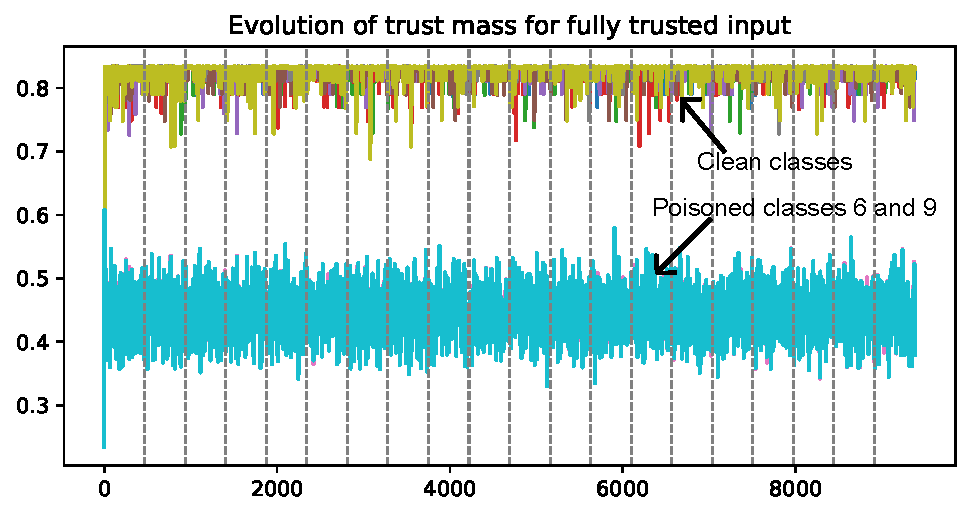
\includegraphics[width=\linewidth]{img/patas/plot_ptas-128-t-t-ps4.pdf}
    \caption{Evolution of trust masses across training rounds (one round corresponds to a feedforward and backpropagation pass).}
    \end{subfigure}
    \begin{subfigure}{0.45\linewidth}
        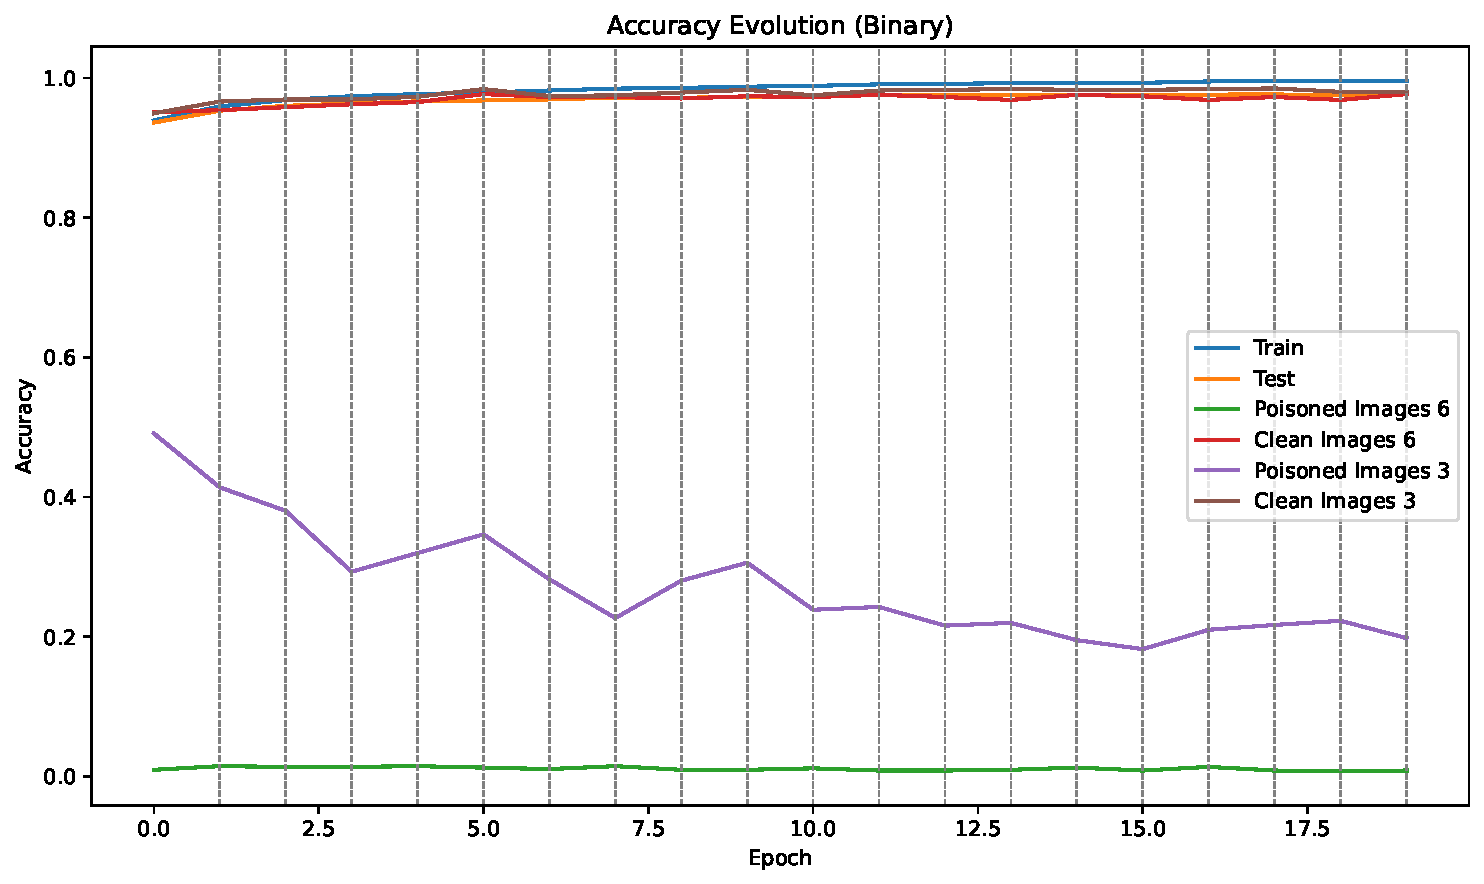
\includegraphics[width=\linewidth]{latex/NN_Train_mnist_128_trust_trust_PathSize_4__accuracy_evolution.pdf}
    \caption{Accuracy}
    \end{subfigure}
    \caption{Evolution of trust mass for fully trusted input in the MNIST poisoned Experiment with patch size \(4\times 4\) pixels}
    \label{fig:4x4}
\end{figure}
The evaluation of the Parallel Trust Assessment System (PaTAS) is conducted during the training phase of the \ac{NN}. After each iteration of training (i.e., a complete feedforward and backpropagation cycle), we assume that an inference is performed, and we assess the trustworthiness of the corresponding output. This assessment is carried out under three input trust profiles:
\begin{itemize}
\item \emph{Fully Trusted Input}: input is considered fully trusted.
\item \emph{Fully Uncertain Input}: input is considered fully uncertain.
\item \emph{Fully Distrusted Input}: input is fully unreliable.
\end{itemize}
We focus on these three profiles because they represent the extreme and most informative boundary cases of input trust. 

For each of these three input types, we track and plot the evolution of three key metrics over the course of training:
\begin{itemize}
\item \emph{Trust Mass}: the level of confidence in the output.
\item \emph{Uncertainty Mass}: the uncertainty of the assessment.
\item \emph{Distrust Mass}: the level of disbelief in the output.
\end{itemize}

As a result, for each evaluation, 9 distinct plots are generated, corresponding to the 3 input types (fully trusted, fully uncertain, and fully distrusted) and each of the three key metrics (trust, uncertainty, and distrust)\footnote{The base rate is set to 0.5 and remains constant across all experiments.}.

All the results are depicted in Figures in the \appp and summarized in \cref{tab:cancer_results,tab:mnist,tab:mnistpois,fig:mnistpoisipta}. They confirm several theoretical properties of \ac{PaTAS-TP} proven in \cref{sec:ptastheory}:



\begin{itemize}
\item \emph{Stability of the trust assessment}: once the gradients of the network have stabilised, the trust assessment stabilises as well, as \cref{thm:convergence} predicts; it keeps fluctuating slightly with the mini-batch evidence.
\item \emph{Inference on fully uncertain input yields fully uncertain output}: a fully uncertain input always produces a fully uncertain output.
\item \emph{Symmetric Inference}: when input trust assessments are symmetric, the inference results remain symmetric.
\end{itemize}

For detailed results, we primarily focus on the three plots for each experiment) corresponding to feedforward of fully trusted input. Processing uncertain inputs naturally yields uncertain outputs, while symmetry implies that trusted and distrusted cases mirror each other. We also confirm that when processing fully trusted inputs, the distrust mass remains close to zero. Since trust, uncertainty, and distrust sum to 1, analyzing only the trust mass is sufficient in such cases. Therefore we keep only the trust mass after the training in \cref{tab:cancer_results,tab:mnist,tab:mnistpois,tab:epsilon_gap}. 

\subsubsection*{Experiment 1 -- Breast Cancer Classification}
\begin{table}[ht]
\resizebox{\textwidth}{!}{%
\begin{tabular}{llcccccc}
\hline
X Trust & Y Trust & $\epsilon=1$ & $\epsilon=0.1$ & $\epsilon=0.01$ & $\epsilon=0.001$ & Train (\%) & Test (\%) \\
\hline
trust & trust & 0.8787 & 0.8787 & 0.6658 & 0.1681 & 98.68 & 96.49 \\
trust & vacuous & 0.3242 & 0.2927 & 0.1290 & 0.0773 & 65.71 & 74.56 \\
trust & distrust & 0.00 & 0.00 & 0.00 & 0.00 & 99.12 & 2.63 \\
vacuous & trust & 0.3392 & 0.3392 & 0.2682 & 0.0931 & 96.70 & 95.61 \\
vacuous & vacuous & 0.3051 & 0.2971 & 0.1820 & 0.1034 & 68.79 & 88.60 \\
vacuous & distrust & 0.00 & 0.00 & 0.00 & 0.00 & 96.92 & 4.39 \\
distrust & trust & 0.00 & 0.00 & 0.00 & 0.00 & 64.62 & 43.86 \\
distrust & vacuous & 0.00 & 0.00 & 0.00 & 0.00 & 56.92 & 33.33 \\
distrust & distrust & 0.00 & 0.00 & 0.00 & 0.00 & 65.49 & 40.35 \\
\hline
\multicolumn{8}{c}{\textit{Extra scenarios}} \\
\hline
(0.25, 0.25, 0.5) & (0.25, 0.25, 0.5) & 0.1172 & 0.1140 & 0.0633 & 0.0272 & 68.79 & 88.60 \\
(0.25, 0.0, 0.75) & (0.25, 0.0, 0.75) & 0.3810 & 0.3809 & 0.2211 & 0.0871 & 80.22 & 95.61 \\
\hline
\end{tabular}%
}
\caption{Summary of final trust mass across four values of $\epsilon$ and corresponding train/test accuracies for the Breast Cancer Classification Experiment (original prototype, one run per cell; a five-seed replication with the released implementation is given in \cref{tab:cancer_seeds}).}
\label{tab:cancer_results}
\end{table}

The results for this experiment are summarized in \cref{tab:cancer_results}. When both features and labels are clean, the model steadily improves and achieves high accuracy (98.68\% training, 96.49\% test), and \ac{PaTAS-TP} produces the highest trust mass across all conditions (0.88 for $\epsilon=0.1$). Clean features with corrupted labels cause test accuracy to collapse to 2.63\%, even while training accuracy remains artificially high at 99.12\%; the model learns the wrong mapping but does so confidently. Correspondingly, trust mass falls to zero regardless of $\epsilon$, correctly signaling the unreliability of the learned parameters. With vacuous labels, performance degrades moderately (65.71\% train, 74.56\% test) and trust mass remains low (0.29). Corrupted features eliminate the ability to learn in any combination: trust mass is zero in all distrust-$X$ rows and test accuracy never exceeds 43.86\%. 

The mild-degradation scenario $(0.25, 0, 0.75)$ for features and labels is the only intermediate case and behaves as expected: with only 15\% of features perturbed and no distrust component, trust mass reaches 0.38 for $\epsilon=0.1$, outperforming every row that uses a fully vacuous opinion for either features or labels. This suggests that an analyst who can bound the degradation and express it as a partial-trust opinion, rather than defaulting to full uncertainty, obtains a more optimistic trust assessment.

We evaluated the system for four values of $\epsilon$ ($0.001, 0.01, 0.1, 1$). We recall that $\epsilon$ is the threshold used by the \textsc{NodeTrust} function in \cref{alg:trustupdate}.
\begin{itemize}
\item For $\epsilon = 0.01$: the system is more sensitive to gradient magnitude. Fully trusted $X$ with trusted $Y$ yields a trust mass of 0.67, while uncertain $Y$ reduces it to 0.13. When $X$ is vacuous, trust stabilizes around 0.27 for trusted $Y$ and 0.18 for uncertain $Y$.
\item For $\epsilon = 0.1$: the larger threshold makes the system less reactive to small gradients. Fully trusted $X$ with trusted $Y$ reaches 0.88; with uncertain $Y$, trust falls to 0.29. Vacuous $X$ with trusted $Y$ yields 0.34, and with uncertain $Y$ yields 0.30. In all cases, distrust in either $X$ or $Y$ drives trust mass to zero.
\end{itemize}

The two additional values clarify the boundary behavior of $\epsilon$. At $\epsilon = 0.001$, the threshold falls well below the typical gradient magnitude during training, causing \textsc{NodeTrust} to classify nearly all gradients as large and therefore as negative evidence; trust mass collapses across all non-distrust configurations, losing the ability to differentiate between trust profiles. At $\epsilon = 1$, the threshold is so permissive that almost all gradients are treated as small, producing results nearly identical to $\epsilon = 0.1$ and offering no additional discriminative power. Among the four values evaluated, $\epsilon = 0.1$ emerges as the most balanced choice, maintaining sensitivity to meaningful gradient activity without collapsing trust mass or losing discriminative power. How $\epsilon$ should be set in practice is discussed in \cref{sec:patas-discussion}.

A notable observation is that the \textit{trust/vacuous} configuration yields a lower trust mass than \textit{vacuous/vacuous} across all values of $\epsilon$ except $\epsilon = 1$. This ordering is consistent with the test accuracies reported in \cref{tab:cancer_results}, where \textit{trust/vacuous} (74.56\%) underperforms \textit{vacuous/vacuous} (88.60\%). The underlying mechanism is that trusted features produce strong, informative gradients that frequently exceed $\epsilon$, generating negative evidence in \textsc{NodeTrust} when labels are unreliable: the model confidently learns from clean features under vacuous supervision, effectively fitting an unreliable mapping. Noisy features, by contrast, produce diffuse gradients that remain below $\epsilon$ more often, partially canceling the effect of uncertain labels and yielding comparatively higher trust mass. This shows that smaller values of $\epsilon$ correctly capture this ordering, while $\epsilon = 1$ is too permissive to discriminate between these regimes and the effect vanishes.

Overall, there is a strong positive correlation between trust mass and test accuracy. Moreover, a smaller $\epsilon$ makes label trust more influential: the relative gap between trusted-$Y$ and uncertain-$Y$ rows, defined as $(T_{\text{trusted}} - T_{\text{uncertain}}) / T_{\text{trusted}}$,
increases as $\epsilon$ decreases, as shown in \cref{tab:epsilon_gap}.
\begin{table}[h]
\centering
\caption{Relative influence of label trust as a function of $\epsilon$,
for trusted and vacuous feature inputs.}
\label{tab:epsilon_gap}

\begin{tabular}{lcccc}
\hline
 & \multicolumn{2}{c}{$\epsilon = 0.1$} & \multicolumn{2}{c}{$\epsilon = 0.01$} \\
\cmidrule(lr){2-3}\cmidrule(lr){4-5}
$X$ trust & $T_{Y=\text{trust}}$ & $T_{Y=\text{vac}}$ & $T_{Y=\text{trust}}$ & $T_{Y=\text{vac}}$ \\
\hline
trusted  & 0.88 & 0.29 & 0.67 & 0.13 \\
vacuous  & 0.34 & 0.30 & 0.27 & 0.18 \\
\hline
\multicolumn{5}{l}{\small Relative gap (trusted): $(0.88-0.29)/0.88 = 67\%$ vs $(0.67-0.13)/0.67 = 81\%$} \\
\multicolumn{5}{l}{\small Relative gap (vacuous): $(0.34-0.30)/0.34 = 12\%$ vs $(0.27-0.18)/0.27 = 33\%$} \\
\hline
\end{tabular}
\end{table}


\paragraph*{Replication across seeds.} \Cref{tab:cancer_results} reports one run per cell, obtained with the original prototype. \Cref{tab:cancer_seeds} repeats the whole grid with the released implementation over five seeds, each seed changing the network initialisation, the batch order and the draw of the degradation, with \ac{PaTAS-TP} attached to a fresh training run for every cell. The replication reproduces every qualitative statement made above and bounds their variability. At $\epsilon = 1$ the trust mass has no variance at all, because every gradient falls below the threshold and the evidence is the same in every batch. At $\epsilon = 0.1$ the trusted configuration gives $0.867 \pm 0.023$ (four of the five seeds give $0.877$ to $0.879$ and one gives $0.820$), the vacuous-feature/trusted-label configuration gives $0.339$ in every seed, and the trusted-feature/vacuous-label configuration gives $0.270 \pm 0.013$. The ordering behind F1.1 holds in all five seeds; so do the reversal between these two rows at $\epsilon = 1$ and the ordering of the vacuous/vacuous row above the trusted/vacuous row at $\epsilon \le 0.1$, and the relative gaps of \cref{tab:epsilon_gap} are reproduced ($69\%$ and $13\%$ at $\epsilon = 0.1$, $81\%$ and $29\%$ at $\epsilon = 0.01$). The mixed opinion $(0.25, 0.25, 0.5)$ lowers the trust mass from $0.295 \pm 0.008$ to $0.113 \pm 0.003$ at identical accuracy (F1.2), and the mild-degradation opinion gives $0.347 \pm 0.025$, above every fully vacuous row but only marginally above the vacuous-feature/trusted-label row. The largest variability is in the test accuracy of the degraded-label and distrusted-feature configurations, where the seed decides which wrong mapping the model learns; the trust mass of those configurations is zero in every seed, as the calculus prescribes.

\begin{table}[ht]
\resizebox{\textwidth}{!}{%
\begin{tabular}{llcccccc}
\hline
X Trust & Y Trust & $\epsilon=1$ & $\epsilon=0.1$ & $\epsilon=0.01$ & $\epsilon=0.001$ & Train (\%) & Test (\%) \\
\hline
trust & trust & 0.879 $\pm$ 0.000 & 0.867 $\pm$ 0.023 & 0.604 $\pm$ 0.116 & 0.145 $\pm$ 0.063 & 98.6 $\pm$ 0.4 & 97.5 $\pm$ 0.7 \\
trust & vacuous & 0.324 $\pm$ 0.000 & 0.270 $\pm$ 0.013 & 0.116 $\pm$ 0.006 & 0.072 $\pm$ 0.005 & 67.2 $\pm$ 3.7 & 76.0 $\pm$ 12.7 \\
trust & distrust & 0.000 $\pm$ 0.000 & 0.000 $\pm$ 0.000 & 0.000 $\pm$ 0.000 & 0.000 $\pm$ 0.000 & 98.5 $\pm$ 0.3 & 2.6 $\pm$ 1.0 \\
vacuous & trust & 0.339 $\pm$ 0.000 & 0.339 $\pm$ 0.000 & 0.252 $\pm$ 0.042 & 0.076 $\pm$ 0.015 & 96.7 $\pm$ 0.4 & 95.4 $\pm$ 0.4 \\
vacuous & vacuous & 0.305 $\pm$ 0.000 & 0.295 $\pm$ 0.008 & 0.179 $\pm$ 0.022 & 0.112 $\pm$ 0.008 & 69.9 $\pm$ 3.0 & 90.7 $\pm$ 3.4 \\
vacuous & distrust & 0.000 $\pm$ 0.000 & 0.000 $\pm$ 0.000 & 0.000 $\pm$ 0.000 & 0.000 $\pm$ 0.000 & 96.6 $\pm$ 0.4 & 4.0 $\pm$ 0.4 \\
distrust & trust & 0.000 $\pm$ 0.000 & 0.000 $\pm$ 0.000 & 0.000 $\pm$ 0.000 & 0.000 $\pm$ 0.000 & 63.4 $\pm$ 0.5 & 51.6 $\pm$ 11.3 \\
distrust & vacuous & 0.000 $\pm$ 0.000 & 0.000 $\pm$ 0.000 & 0.000 $\pm$ 0.000 & 0.000 $\pm$ 0.000 & 57.8 $\pm$ 1.1 & 54.9 $\pm$ 17.7 \\
distrust & distrust & 0.000 $\pm$ 0.000 & 0.000 $\pm$ 0.000 & 0.000 $\pm$ 0.000 & 0.000 $\pm$ 0.000 & 63.5 $\pm$ 1.2 & 64.4 $\pm$ 13.9 \\
\hline
\multicolumn{8}{c}{\textit{Extra scenarios}} \\
\hline
(0.25, 0.25, 0.5) & (0.25, 0.25, 0.5) & 0.117 $\pm$ 0.000 & 0.113 $\pm$ 0.003 & 0.063 $\pm$ 0.008 & 0.030 $\pm$ 0.002 & 69.9 $\pm$ 3.0 & 90.7 $\pm$ 3.4 \\
(0.25, 0.0, 0.75) & (0.25, 0.0, 0.75) & 0.381 $\pm$ 0.000 & 0.347 $\pm$ 0.025 & 0.197 $\pm$ 0.038 & 0.102 $\pm$ 0.016 & 81.9 $\pm$ 0.9 & 94.6 $\pm$ 1.0 \\
\hline
\end{tabular}%
}
\caption{Five-seed replication of \cref{tab:cancer_results} with the released implementation (mean $\pm$ standard deviation over five seeds; each seed changes the initialisation, the batch order and the degradation draw, and the network is retrained for every cell). Accuracies do not depend on $\epsilon$.}
\label{tab:cancer_seeds}
\end{table}

\paragraph*{Sensitivity to the batch size.} Since the batch label opinion of \cref{alg:trustupdate} is a mean, the batch size affects the parameter trust only through the gradient evidence: the number of revision steps per epoch and the gradient noise both change with the batch size, and so does the count of gradients below $\epsilon$. \Cref{tab:cancer_batch} reports the trust mass and the mean parameter opinion of the first layer for batch sizes from 8 to 256 (released implementation, $\epsilon = 0.1$, three seeds). Under trusted data the trust mass is flat, between $0.876$ and $0.879$ for every batch size, except for one of the three seeds at batch size 64, which yields $0.820$ (the same run appears in \cref{tab:cancer_seeds}); the mean parameter uncertainty of the first layer stays close to the fixed point of \cref{thm:convergence} ($u_q/15 = 0.004$ for $31$ incoming edges; measured $0.005$). Under vacuous data the trust mass varies by $0.023$ (from $0.282$ to $0.305$) across a 32-fold range of batch sizes, and with trusted features and vacuous labels by $0.05$, the largest batches giving the highest trust mass because batch-averaged gradients are smoother and more often fall below $\epsilon$. The batch size is therefore a second-order factor, and the values of \cref{tab:cancer_results} are reported for the batch size of 64 used in training.

\begin{table}[ht]
\centering
\begin{tabular}{crrrr}
\hline
Batch size & \multicolumn{2}{c}{trust / trust} & vacuous / vacuous & trust / vacuous \\
 & Trust mass & $(b, d, u)$ of layer 1 & Trust mass & Trust mass \\
\hline
8   & $0.876 \pm 0.002$ & $(0.993, 0.002, 0.005)$ & $0.285 \pm 0.007$ & $0.278 \pm 0.028$ \\
16  & $0.877 \pm 0.002$ & $(0.994, 0.001, 0.005)$ & $0.282 \pm 0.009$ & $0.272 \pm 0.018$ \\
32  & $0.878 \pm 0.001$ & $(0.995, 0.000, 0.005)$ & $0.287 \pm 0.006$ & $0.269 \pm 0.027$ \\
64  & $0.859 \pm 0.027$ & $(0.994, 0.001, 0.005)$ & $0.291 \pm 0.008$ & $0.276 \pm 0.011$ \\
128 & $0.879 \pm 0.000$ & $(0.995, 0.000, 0.005)$ & $0.305 \pm 0.000$ & $0.315 \pm 0.006$ \\
256 & $0.877 \pm 0.000$ & $(0.993, 0.000, 0.006)$ & $0.305 \pm 0.000$ & $0.322 \pm 0.003$ \\
\hline
\end{tabular}
\caption{Sensitivity of the trust mass to the training batch size on the breast-cancer task (released implementation, $\epsilon = 0.1$, 15 epochs, mean $\pm$ standard deviation over three seeds). The $(b, d, u)$ column is the mean parameter opinion of the first layer under trusted data.}
\label{tab:cancer_batch}
\end{table}

\begin{tcolorbox}[title=Key findings -- Experiment 1, colback=gray!5, colframe=gray!40, fonttitle=\bfseries, left=4pt, right=4pt, top=4pt, bottom=4pt]
\textbf{F1.1 Label trust matters more than feature trust on this task.} Setting $X$ as vacuous
while keeping $Y$ trusted yields a higher trust mass (0.34) than the reverse
(0.29 for trusted $X$, uncertain $Y$); the ordering holds in all five seeds of the
replication (\cref{tab:cancer_seeds}). It is a statement about one dataset and about
degradations assigned jointly with the opinions, not a general law: the label opinion
enters the auxiliary sub-step of every layer, whereas the feature opinion enters the
first layer directly and the deeper layers only through propagation.

\medskip
\textbf{F1.2 Distrust is more damaging than uncertainty.} Replacing a fully
uncertain opinion $(0,0,1)$ for both $X$ and $Y$ with a mixed assessment
$(0.25, 0.25, 0.5)$ reduces trust mass from 0.30 to 0.11, while accuracy
remains unchanged (88.60\%), confirming the drop is driven by the distrust
component alone.

\medskip
\textbf{F1.3 Finer $\epsilon$ amplifies label-trust sensitivity.} As shown in
\cref{tab:epsilon_gap}, the relative gap between trusted-$Y$ and uncertain-$Y$
is larger for $\epsilon=0.01$ than for $\epsilon=0.1$, in both the trusted and
vacuous feature settings.
\end{tcolorbox}














\subsubsection*{Experiment 2 -- MNIST Dataset}
\begin{table}
\centering
\begin{tabular}{cccccc}
\hline
Architecture & X Trust & Y Trust & Trust Mass & Train Acc (\%) & Test Acc (\%) \\
\hline
16 & vacuous & vacuous & 0.3087 & 65.19 & 73.96 \\
32 & vacuous & vacuous & 0.3224 & 66.20 & 79.03 \\
64 & vacuous & vacuous & 0.3306 & 67.22 & 89.98 \\
128 & vacuous & vacuous & 0.3359 & 67.78 & 92.05 \\
16-16 & vacuous & vacuous & 0.1628 & 65.68 & 69.39 \\
16 & trust & trust & 0.8620 & 96.37 & 95.13 \\
16-16 & trust & trust & 0.7077 & 96.83 & 95.84 \\
\hline
\end{tabular}
\caption{Summary of final trust mass for the MNIST Classification Experiment (original prototype, one run per row; a three-seed replication with the released implementation is given in \cref{tab:mnist_seeds}).}
\label{tab:mnist}
\end{table}
In this experiment, \ac{PaTAS-TP} produces ten output trust opinions, one for each class. However, they are almost identical across classes, so we record only the aggregated trust mass in \cref{tab:mnist}.

When features and labels are vacuous, accuracy improves as model size increases, from 73.96\% (architecture 16) to 92.05\% (architecture 128). Test accuracy exceeds training accuracy in every vacuous row. This is not an effect of \ac{PaTAS-TP}, which never modifies the training: the vacuous profile is realised by injecting feature and label noise into the training set only, so the training accuracy is measured on degraded samples and partly corrupted labels, while the test set is clean. Trust mass follows the same upward trend with model size (0.3087, 0.3224, 0.3306, 0.3359), though the gains become progressively smaller, indicating diminishing returns from added capacity under uncertain data.

The two-layer architecture (16-16) is a notable exception. Despite having more parameter count than the single-layer 16-hidden neurons network, it yields a trust mass of only 0.1628 under vacuous inputs and 0.7077 under trusted inputs, both consistently lower than the single-layer 16-neuron counterpart (0.3087 and 0.8620 respectively). This is not an artifact but a meaningful property of the framework: each additional layer introduces an extra round of trust discounting, which attenuates the trust signal propagating through the network. A deeper architecture therefore inherits less trust from its inputs, even when those inputs are reliable. This behavior is consistent with \ac{PaTAS-TP} design, since a deeper inference path involves more parameters, each contributing uncertainty, and the framework correctly reflects that the output trust depends on the full chain of parameter reliability. A secondary factor is convergence speed: the gradients of the deeper network stabilise later, and since the parameter trust is a running mean of the recent gradient evidence (\cref{thm:convergence}), it is still moving when training stops.

The trusted evaluation provides the clearest contrast. Architecture 16 with trusted features and labels reaches a trust mass of 0.8620, far exceeding any vacuous-data configuration regardless of architecture size. Even the deeper 16-16 architecture achieves 0.7077 under trusted inputs, outperforming the largest single-layer architecture (128, trust mass 0.3359) trained under vacuous data by a wide margin. On this dataset, data quality thus has a far greater impact on the resulting trust assessment than model capacity; part of this ordering is designed in, since the vacuous profile also degrades the data the model learns from.

\paragraph*{Replication across seeds.} \Cref{tab:mnist} reports one run per row, obtained with the original prototype. \Cref{tab:mnist_seeds} repeats the seven configurations with the released implementation over three seeds, each seed changing the initialisation, the batch order and the noise draw, with \ac{PaTAS-TP} attached to a fresh training run. The trust masses of the vacuous rows are reproduced to within $0.01$ of \cref{tab:mnist}, the trusted rows to within $0.05$ (the released implementation gives $0.842 \pm 0.011$ for the 16-neuron network and $0.696 \pm 0.028$ for the 16-16 network under trusted data). The width ordering of F2.1 holds in every seed, with a total gain from 16 to 128 neurons of $0.030 \pm 0.004$ that exceeds the seed dispersion of every row. The depth penalty of F2.2 holds in every seed under both profiles ($0.162 \pm 0.003$ against $0.306 \pm 0.004$ under vacuous data, $0.696 \pm 0.028$ against $0.842 \pm 0.011$ under trusted data). The test accuracy exceeds the training accuracy in every vacuous run, for the reason given above, and it is the quantity with the largest seed dispersion.

\begin{table}[ht]
\centering
\begin{tabular}{cccccc}
\hline
Architecture & X Trust & Y Trust & Trust Mass & Train Acc (\%) & Test Acc (\%) \\
\hline
16 & vacuous & vacuous & $0.3057 \pm 0.0038$ & $65.66 \pm 0.19$ & $79.53 \pm 6.51$ \\
32 & vacuous & vacuous & $0.3217 \pm 0.0028$ & $67.09 \pm 0.13$ & $82.83 \pm 3.43$ \\
64 & vacuous & vacuous & $0.3309 \pm 0.0013$ & $67.89 \pm 0.13$ & $88.75 \pm 1.55$ \\
128 & vacuous & vacuous & $0.3355 \pm 0.0007$ & $68.38 \pm 0.15$ & $91.96 \pm 1.56$ \\
16-16 & vacuous & vacuous & $0.1618 \pm 0.0033$ & $66.32 \pm 0.33$ & $80.70 \pm 4.04$ \\
16 & trust & trust & $0.8416 \pm 0.0106$ & $96.60 \pm 0.19$ & $95.62 \pm 0.14$ \\
16-16 & trust & trust & $0.6964 \pm 0.0284$ & $96.79 \pm 0.13$ & $95.24 \pm 0.17$ \\
\hline
\end{tabular}
\caption{Three-seed replication of \cref{tab:mnist} with the released implementation ($\epsilon = 0.05$; mean $\pm$ standard deviation over three seeds; each seed changes the initialisation, the batch order and the noise draw).}
\label{tab:mnist_seeds}
\end{table}

\begin{tcolorbox}[title=Key findings -- Experiment 2, colback=gray!5,
colframe=gray!40, fonttitle=\bfseries, left=4pt, right=4pt,
top=4pt, bottom=4pt]

\textbf{F2.1 Trust increases with model width, with diminishing returns.} Under vacuous data, trust mass grows from 0.3087 (16 neurons) to 0.3359 (128 neurons), but the incremental gain shrinks at each step, suggesting that additional capacity provides less benefit once the dominant bottleneck is data quality rather than model expressiveness.

\medskip
\textbf{F2.2 Depth penalises trust due to discounting accumulation.} The 16-16 architecture consistently yields lower trust than the single-layer 16-neuron network under both vacuous (0.1628 vs.\ 0.3087) and trusted (0.7077 vs.\ 0.8620) inputs. Each additional layer introduces an extra discounting step, so deeper networks attenuate the trust signal regardless of their predictive accuracy.

\medskip
\textbf{F2.3 Data quality dominates model capacity for trust on this benchmark.} Training the smallest architecture on trusted data (trust mass 0.8620) far exceeds training the largest architecture on vacuous data (trust mass 0.3359). The comparison is confined to one dataset and to trust profiles that are assigned jointly with the degradations, so it should be read as a property of the calculus under correct opinions rather than as a general empirical law.
\end{tcolorbox}


\subsubsection*{Experiment 3 -- Poisoned MNIST Dataset}
\begin{table}[ht]
\centering
\resizebox{\textwidth}{!}{
\begin{tabular}{ccccccccc}
\hline
Patch size & Trust for 3 & Trust for 6 & Train (\%) & Test (\%) & Clean 3 (\%) & Clean 6 (\%) & 3 with patch (\%) & 6 with patch (\%) \\
\hline
$(1 \times 1)$   & 0.836 & 0.440 & 99.62 & 97.66 & 97.72 & 97.49 & 83.76 & 0.63 \\
$(4 \times 4)$   & 0.833 & 0.439 & 99.62 & 97.66 & 98.02 & 97.70 & 19.80 & 0.84 \\
$(10 \times 10)$ & 0.815 & 0.433 & 99.60 & 97.61 & 97.62 & 97.49 & 16.44 & 0.63 \\
$(27 \times 27)$ & 0.651 & 0.386 & 96.35 & 97.73 & 98.02 & 97.81 &  0.00 & 0.00 \\
\hline
\end{tabular}
}
\caption{Summary of results for the Poisoned MNIST Classification Experiment.}
\label{tab:mnistpois}
\end{table}


\begin{figure}
    \centering
    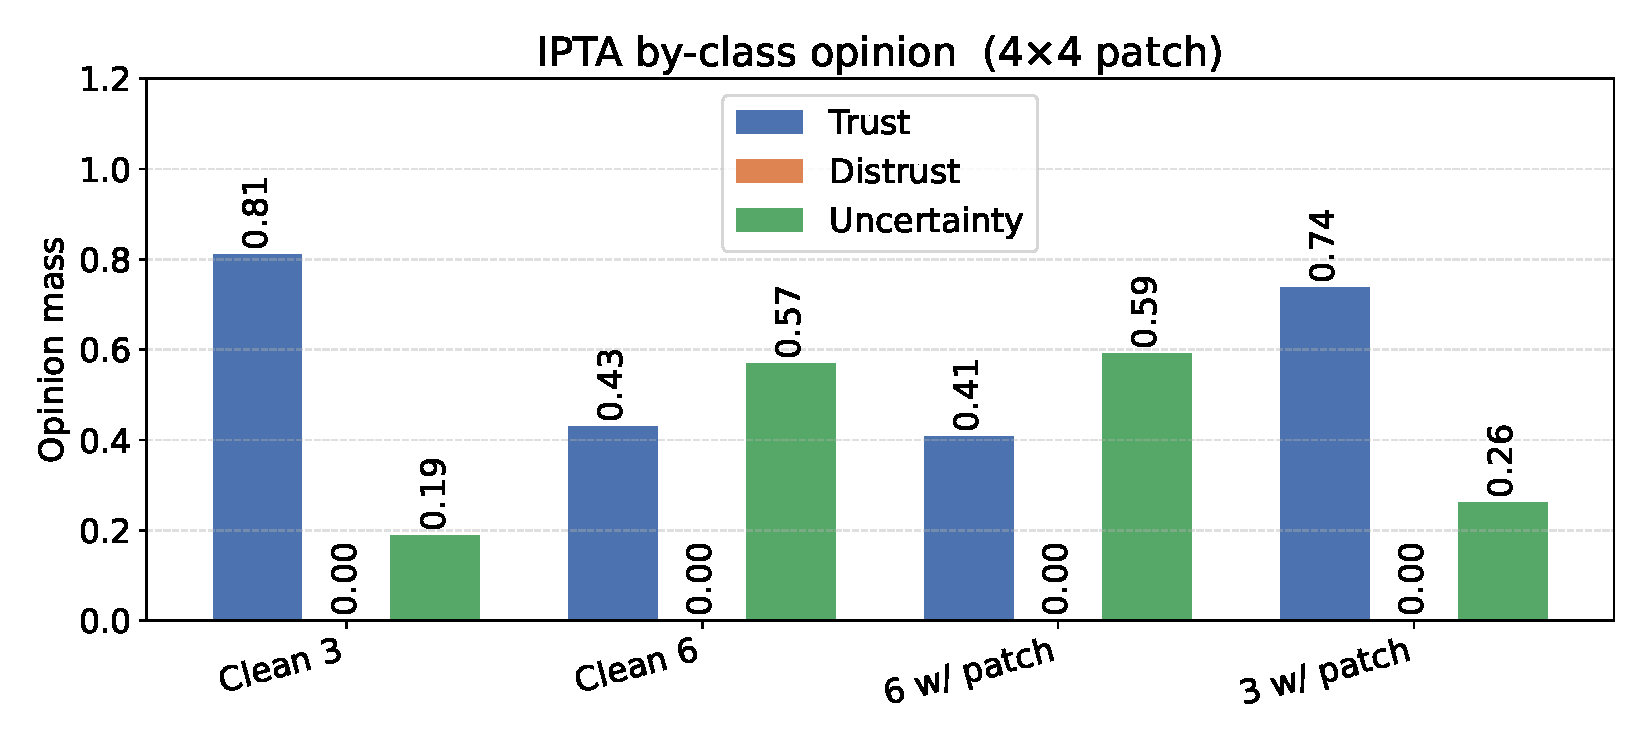
\includegraphics[width=0.8\linewidth]{latex/NN_Train_mnist_128_trust_trust_PathSize_4__ipta_table2a.pdf}
    \caption{\ac{IPTA} results for \ac{NN} trained on poisoned datasets with patch size $4 \times 4$. Results are obtained by feedforwarding a fully trusted opinion, except the patch-distrusted, where patch pixels are explicitly assigned distrust.}
    \label{fig:mnistpoisipta}
\end{figure}

\begin{table}[h]
\centering
\caption{Relative trust gap between clean label 3 and poisoned label 6
as a function of patch size.}
\label{tab:reldrop}
\begin{tabular}{lccc}
\hline
Patch size & $T_3$ & $T_6$ & $(T_3 - T_6)/T_3$ (\%) \\
\hline
$1\times1$   & 0.836 & 0.440 & 47.4 \\
$4\times4$   & 0.833 & 0.439 & 47.3 \\
$10\times10$ & 0.815 & 0.433 & 46.9 \\
$27\times27$ & 0.651 & 0.386 & 40.7 \\
\hline
\end{tabular}
\end{table}

As in the previous experiment, \ac{PaTAS-TP} produces ten output trust opinions. In \cref{tab:mnistpois} we report the trust mass for label 3 (a clean class) and label 6 (a poisoned class), alongside overall train/test accuracy and per-class accuracy on both clean and patched test samples.

Across all patch sizes, the trust mass for label 3 consistently exceeds that for label 6 (e.g.\ 0.836 vs.\ 0.440 for the $1\times1$ patch), confirming that \ac{PaTAS-TP} reliably distinguishes clean from poisoned labels even when overall accuracy remains high (97.66\%). As the patch grows, both trust values decrease, but not symmetrically: as shown in \cref{tab:reldrop}, the relative gap $(T_3 - T_6)/T_3$ decreases with patch size, from 47.4\% at $1\times1$ down to 40.7\% at $27\times27$, indicating that larger patches erode the trust advantage of the clean class more than they further penalize the already-distrusted poisoned class. As a result, the gap between the two patches decreases with patch size. This asymmetry is interpretable: as the patch occupies a larger fraction of the image, the underlying model increasingly associates the patch pattern directly with the target poisoned class, bypassing the remaining image features. The parameters involved in clean-class prediction are therefore affected more by the growing patch than those already conditioned on the poisoned signal, which partially absorbs the patch regardless of its size. The clear separation between the two classes is nonetheless maintained across all patch sizes.

Regarding classification accuracy, patched digit 6 samples are almost entirely misclassified regardless of patch size ( $\leq$ 0.84\%), confirming the backdoor
attack is effective. Patched digit 3 accuracy degrades more gradually, dropping
sharply from 83.76\% at $1\times1$ to roughly 16 to 20\% for larger patches,
reflecting the spatial overlap between the patch and discriminative features for
digit 3. The $27\times27$ case is an edge case rather than a realistic poisoning
scenario: a patch of this size dominates the entire image at inference time, so
the model associates the input almost entirely with the poisoned trigger rather
than the digit. One of the poisoned classes therefore reaches near-100\% accuracy
while the other collapses to 0\%, producing the 0\% accuracy observed for both
patched digits 3 and 6. This extreme case is included only to illustrate the
boundary behavior of the framework.

To evaluate the \ac{IPTA}, \cref{fig:mnistpoisipta} reports accuracy and the full trust opinion $(t, d, u)$ for clean and patched samples, obtained by feedforwarding a fully trusted opinion through the \ac{IPTA} instantiated from the respective inference path in the $4\times 4$ patch model. As established in \cref{thm:infvac} (\cref{rem:directional}), feedforwarding a fully trusted input $(1, 0, 0)$ through any \ac{PaTAS-TP} configuration yields an output with zero distrust mass, since the discounting operator maps a fully trusted input to an opinion with $d=0$, and fusion preserves this zero mass. This is confirmed across all rows using a trusted $T_x$: distrust remains exactly 0 in every case.

Clean digit 3 achieves the strongest trust profile (0.811 trust, 0.189 uncertainty), consistent with high accuracy (98.02\%). Clean digit 6 already exhibits markedly higher uncertainty (0.570) despite comparable accuracy (97.70\%), reflecting that the parameters on the digit-6 inference path were exposed to poisoned training samples and are therefore less trusted.

For patched samples, the degradation is clear. Patched digit 6 accuracy collapses to 0.84\% and trust drops to 0.408, with uncertainty dominating at 0.592, providing a warning signal unavailable from accuracy alone. For patched digit 3, accuracy falls to 19.80\% yet trust remains relatively higher at 0.738, reflecting that the digit-3 inference path passes through less poisoned parameters. A replication of this setup with the released implementation, ten independent trainings with different seeds, confirms that the gap is robust: mean \ac{IPTA} belief $0.884 \pm 0.001$ for the clean class against $0.503 \pm 0.036$ for the poisoned class (\cref{tab:pois_provenance}). This experiment relies on two simplifying assumptions: the patch location is known when the trust opinions are assigned, and the patch and the label flip are always applied together. Experiment~4 revisits the same poisoning without either assumption; it estimates the input opinions from the data and separates the two corruption channels.

\paragraph*{Provenance of the poisoned-MNIST trust values.} The clean-class and poisoned-class trust values quoted for this setup differ across the chapter because they come from two implementations, two ways of feeding the input, and two metrics. \Cref{tab:pois_provenance} lists them; all refer to the $4\times4$ patch and the 784-128-10 architecture. The values agree once the metric and the input route are taken into account: the projected probability of \cref{tab:diss-classtrust} ($0.947$ and $0.756$) approximately equals $b + u/2$ of the corresponding replication opinion ($0.884 + 0.116/2 = 0.942$ and $0.503 + 0.497/2 = 0.752$), the small difference coming from the input route, since \cref{tab:diss-classtrust} feeds the full network whereas the replication feeds the \ac{IPTA} path of each sample.

\begin{table}[ht]
\centering
\resizebox{\textwidth}{!}{%
\begin{tabular}{llllcc}
\hline
Reported in & Implementation & Input opinion & Metric & Clean class (3) & Poisoned class (6) \\
\hline
\cref{tab:mnistpois} & original prototype, one run & fully trusted, full network & belief $b$ of the class output opinion & 0.833 & 0.439 \\
\cref{fig:mnistpoisipta} & original prototype, one run & fully trusted, \ac{IPTA} of the sample's path & belief $b$ & 0.811 & 0.430 \\
Replication (text above) & released, 10 trainings & fully trusted, \ac{IPTA} of the sample's path & belief $b$, mean $\pm$ std & $0.884 \pm 0.001$ & $0.503 \pm 0.036$ \\
Experiment~4 & released, one run & fully trusted, \ac{IPTA} of the sample's path & belief $b$, mean over 400 clean samples & 0.886 & 0.508 \\
Experiment~4 & released, one run & conformity opinions, \ac{IPTA} & belief $b$, mean over 400 clean samples & 0.779 & 0.444 \\
Experiment~4 & released, one run & oracle patch-distrust opinions, \ac{IPTA} & belief $b$, mean over 400 clean samples & 0.870 & 0.498 \\
\cref{tab:diss-classtrust} & released, one run & fully trusted, full network & projected probability $b + u/2$ & 0.947 & 0.756 \\
\hline
\end{tabular}%
}
\caption{Provenance of the trust values reported for the $4\times4$ poisoned MNIST setup (784-128-10; $\epsilon = 0.05$ for the released implementation). Class~6 is one of the two flipped classes; \cref{tab:diss-classtrust} reports both flipped classes.}
\label{tab:pois_provenance}
\end{table}

\begin{tcolorbox}[title=Key findings -- Experiment 3, colback=gray!5,
colframe=gray!40, fonttitle=\bfseries, left=4pt, right=4pt,
top=4pt, bottom=4pt]

\textbf{F3.1 Trust separates clean from poisoned inference paths.} Across all patch sizes, the trust mass for label 3 (clean) consistently exceeds that for label 6 (poisoned), even when overall test accuracy remains above 97\%. \ac{PaTAS-TP} therefore reveals reliability differences that accuracy alone cannot expose.

\medskip
\textbf{F3.2 Larger patches narrow the trust gap by affecting clean paths
more than poisoned ones.} As patch size grows, the trust mass for the clean label decreases more steeply than for the poisoned label. The model increasingly relies on the patch pattern rather than image features, which degrades the parameters along clean-class inference paths more than those already conditioned on
the poisoned signal.

\medskip
\textbf{F3.3 Zero distrust under trusted input is theoretically guaranteed.} When the input trust is fully trusted $(1,0,0)$, distrust in the output is exactly zero, as established in \cref{thm:infvac}. This is confirmed empirically across all IPTA rows using trusted $T_x$.
\end{tcolorbox}

These results demonstrate that \ac{PaTAS-TP} not only correlates with accuracy but provides complementary information: it identifies which inference paths are structurally less reliable, responds to the size of adversarial corruption, and distinguishes clean from poisoned classes even when overall accuracy remains high.

\subsubsection*{Experiment 4 -- Comparative Trust Evaluation}

\paragraph*{In-distribution behavior.}
On clean test data the composed score matches the maximum-softmax filter on correct-versus-incorrect discrimination (AUROC $0.979 \pm 0.003$ for both on MNIST), with equal calibration error after identical post-hoc calibration: when nothing violates the training distribution, trust-weighting costs nothing. Under corruption the two signals separate \emph{by design}: accuracy barely drops on the robust MLP, so the softmax retains a higher correct-versus-incorrect AUROC on the mixed batch ($0.974$ vs.\ $0.895$) precisely because it ignores the distribution violation that the trust factor flags. Confidence ranks correctness within the training distribution; trust exposes inputs that leave it. The detection tasks below measure the latter.

\begin{table}[ht]
\centering
\resizebox{\textwidth}{!}{%
\begin{tabular}{lcccccc}
\hline
 & OOD M$\to$F & Det.\ MNIST & Det.\ F-MNIST & OOD F$\to$M & Shift & Blend \\
Method & AUROC & AUROC & AUROC & AUROC & AUROC & AUROC \\
\hline
PaTAS (composed) & 0.975 & 0.972 & 0.835 & 0.781 & \textbf{0.781} & 0.564 \\
Conformity alone & \textbf{1.000} & \textbf{1.000} & \textbf{0.994} & 0.481 & 0.678 & 0.500 \\
Mahalanobis (pixel) & 0.997 & 0.997 & 0.944 & 0.942 & 0.716 & 0.482 \\
kNN (pixel) & 0.965 & 0.603 & 0.707 & 0.967 & 0.749 & 0.500 \\
Mahalanobis (feature) & 0.978 & 0.743 & 0.785 & \textbf{0.988} & 0.783 & 0.474 \\
kNN (feature) & 0.994 & 0.588 & 0.625 & 0.973 & \textbf{0.801} & 0.508 \\
Energy score & 0.850 & 0.636 & 0.603 & 0.873 & 0.707 & 0.541 \\
Max softmax & 0.883 & 0.631 & 0.558 & 0.805 & 0.740 & 0.566 \\
MC Dropout & 0.936 & 0.621 & 0.545 & 0.834 & 0.747 & 0.574 \\
\ac{EDL} & 0.883 & 0.547 & 0.510 & 0.767 & 0.736 & 0.561 \\
\hline
\end{tabular}%
}
\caption{Detection of distribution violations (mean over three evaluation seeds, dispersion at most $\pm 0.005$): \ac{OOD} detection in both directions between MNIST and Fashion-MNIST, clean-versus-corrupted separation on the mixed batches (uniform feature noise), and the two hard MNIST corruptions (marginal-preserving translation; low-amplitude blended center trigger). The blended trigger defeats every method (best entry $0.574$), a limit shared by all ten scores against an adversary that stays inside the per-feature range.}
\label{tab:diss-detection}
\end{table}

\paragraph*{Detection and attribution.}
\Cref{tab:diss-detection} reports the violation-detection tasks. Three mechanisms are cleanly separable. First, \emph{violation detection is carried by input-space signals}: the conformity opinions are perfect or near-perfect where inputs violate the training marginals (\ac{OOD} M$\to$F $1.000$, corruption detection $1.000$ and $0.994$), the raw-pixel Mahalanobis baseline is close behind, and an ablation replacing the conformity opinions with the constant fully trusted opinion collapses the composed score to the output-only level ($0.896$ and $0.639$ on the forward tasks, single-seed). Trust propagation is not the detector; it is the carrier that turns the detection signal into an opinion composable with model trust. Second, \emph{propagation contributes exactly where the input marginals are silent}: under the marginal-preserving translation the conformity score drops to $0.678$ as predicted by its construction, while the composed score reaches $0.781$, above its own input factor, because translated inputs traverse atypical activation paths that the \ac{IPTA} reads as less trusted. Third, \emph{the directions of failure are principled}: in the subset direction (Fashion-MNIST model, MNIST digits as \ac{OOD}), digits occupy a quiet subset of the clothing marginals rather than violating them, the conformity score collapses below chance ($0.481$), and the neighborhood- and covariance-based detectors own the task ($0.988$ feature Mahalanobis, $0.942$ pixel Mahalanobis). The composition fails safely there: the confidence factor keeps the composed score at the output-baseline level ($0.781$ vs.\ $0.805$ softmax) instead of inheriting the collapse. Since the subset-direction signal demonstrably exists in input space, mapping such a detector through the same quantification into an additional input opinion is a natural \ac{SL} extension, left as future work.

On the applicability-boundary case, GTSRB, the marginal conformity model detects corruption only weakly ($0.645$; composed $0.545$), exactly as the diagnostics of \cref{sec:conformity} predict (\cref{tab:diss-diagnostics}: no witness features with $w_j \geq 4$). The pixel-space Mahalanobis baseline still reaches $0.997$ on the same task: the boundary belongs to the per-feature marginal model, not to input-space assessment as such, which sharpens the diagnostics into an actionable gate: when they flag a domain, a covariance-aware input model is required.

\begin{table}[ht]
\centering
\begin{tabular}{lccccc}
\hline
Dataset & Med.\ $\sigma_{\mathrm{eff}}$ & $w_{\max}$ & Top-10\% & $w{\geq}4$ & Det. \\
\hline
MNIST & 0.47 & 52.3 & 0.32 & 0.40 & 0.972 \\
Fashion-MNIST & 0.90 & 64.0 & 0.76 & 0.18 & 0.835 \\
GTSRB & 0.98 & 1.8 & 0.14 & 0.00 & 0.545 \\
CIFAR-10 (gray) & 0.23 & 1.1 & 0.11 & 0.00 & -- \\
\hline
\end{tabular}
\caption{A-priori applicability diagnostics of the conformity model, computed on clean training features before any model is trained (median effective deviation, maximum reliability weight, weight share of the top decile, fraction of features with $w_j \geq 4$), against the composed score's corruption detection later observed. Registered domains concentrate evidence in reliable witnesses; unregistered imagery has none, and the input-side signal is predicted, and confirmed, to be uninformative there.}
\label{tab:diss-diagnostics}
\end{table}

\paragraph*{Poisoning without an oracle.}
The conformity opinions remove the oracle assumption of Experiment~3. Fed unchanged into the poisoned model's \ac{IPTA}, they flag patched inputs with no knowledge of the trigger: the input trust alone separates clean from patched inputs at AUROC $1.000$ for both classes, because the patch violates the near-constant border features the conformity model weights most, and the parameter-side gap between the clean and the poisoned class persists under these estimated opinions: the mean belief of the true-class output opinion over 400 clean test samples per class is $0.779$ for the clean class against $0.444$ for the poisoned class under the conformity opinions, $0.870$ against $0.498$ under the oracle patch-distrust assignment, and $0.886$ against $0.508$ under a fully trusted input (\cref{tab:pois_provenance}). These are the values of the stored evaluation run of the released implementation on one trained poisoned model; the poisoned-class values move by a few hundredths between trainings of the same setup, within the seed dispersion of the replication ($\pm 0.036$), while the gap to the clean class does not. The remaining assumption, a clean feature source for the conformity fit, degrades gracefully: fitting on the poisoned training set itself still detects the trigger at $0.73$ and $0.67$ per class, while a naive robust fit (median and MAD) does not recover ($0.65$), since MNIST pixel marginals are zero-inflated; contamination-aware conformity fits are explicit future work.

\paragraph*{Separating the corruption channels.}
Experiment~3 applies patch and label flip jointly. Single-channel controls retrained with the $4\times4$ patch separate their effects on the per-class output trust (\cref{tab:diss-classtrust}): under the full backdoor both flipped classes carry an identical trust deficit ($0.756$ for digits 6 and 9 alike, $0.19$ below the minimum of the eight clean classes, whose spread is below $0.001$); the label-flip-only control reproduces nearly the full drop ($0.748$), the patch-only control still produces a clearly detectable deficit ($0.788$), and the unpoisoned model shows no false alarm (both classes at the clean level $0.994$). The trust deficit is therefore pair-specific, symmetric across the flipped pair, driven primarily by the label channel, and present for a purely spurious trigger even when every label is correct.

\begin{table}[ht]
\centering
\begin{tabular}{lcccc}
\hline
Training condition & Clean-class mean & Clean-class min & Trust$_6$ & Trust$_9$ \\
\hline
Unpoisoned & 0.994 & 0.994 & 0.994 & 0.994 \\
Full backdoor (patch + flip) & 0.947 & 0.946 & 0.756 & 0.756 \\
Label flip only & 0.947 & 0.947 & 0.748 & 0.747 \\
Trigger patch only & 0.948 & 0.948 & 0.788 & 0.788 \\
\hline
\end{tabular}
\caption{Per-class output trust (projected probability under a fully trusted input) for the $4\times4$ poisoned MNIST setup and its single-channel controls (784-128-10). Both flipped classes drop identically and far outside the clean-class band; the label channel carries most of the deficit, and the spurious patch alone remains detectable.}
\label{tab:diss-classtrust}
\end{table}

\paragraph*{Training-quality audit.}
The model-side trust provides a training-quality audit that requires no test data at all (\cref{tab:diss-audit}). Under increasing train-time label-flip rates $p$, the feedforward trust under a fully trusted input drops by $31.7\%$ relative to the clean-trained model at \emph{any} non-zero rate, including $p = 0.1$ where test accuracy moves by only three points: a corruption tripwire read from the trained trust state alone. The flat level is designed saturation, not an artifact: at $p = 0.1$ essentially every training batch already contains corrupted labels, so every batch delivers the large-gradient corrections that \textsc{NodeTrust} counts as negative evidence, and the converged trust registers \emph{that} corruption is present rather than how much. When the algorithm instead consumes rate-informed label opinions $T_y = (1{-}p, 0, p)$, the same machinery grades monotonically ($0.951 \to 0.805$): tripwire versus graded meter is a property of the label opinion's informativeness, not of the calculus. The scale-tied threshold of \cref{sec:param_update} preserves the tripwire without any tuning: at $\epsilon_{\mathrm{layer}} = 0.5 \cdot \mathrm{median}(|\delta|)$ the clean model reads $0.625$ against a flat $0.545$ to $0.550$ at every non-zero rate, a margin more than ten times the within-rate spread, while the same rule instantiates thresholds from $5 \cdot 10^{-5}$ (MNIST) to $3 \cdot 10^{-3}$ (breast cancer) across layers and tasks and preserves the trust ordering of the cancer grid. Data-centric baselines bound the comparison in both directions: the fraction of training labels disagreeing with confident predictions recovers $p$ almost exactly and mean training loss grades likewise, but both require retaining the training data at audit time, and mean confidence measures severity but needs clean held-out data.

A dead-unit confound check completes the audit's validation. At every flip rate, no hidden unit is inactive on more than $99\%$ of inputs (dead-unit fraction $0.0\%$), the mean trust of active units itself drops from $0.9999$ to $0.626$ at any non-zero rate, an activity-weighted variant of the audit that removes low-activity units' contribution by construction reproduces the standard audit to within $0.001$ at every rate, and the correlation between unit activation frequency and unit trust is essentially zero. The audit signal lives in the live paths of the network; it does not measure network degeneration.

\begin{table}[ht]
\centering
\begin{tabular}{cccccccc}
\hline
$p$ & Acc.\ (\%) & Conf. & Trust & Trust$_{\mathrm{inf}}$ & Trust$_{\mathrm{auto}}$ & Disagree & Train loss \\
\hline
0   & 97.9 & 0.981 & 0.998 & 0.998 & 0.625 & 0.001 & 0.014 \\
0.1 & 94.7 & 0.841 & 0.682 & 0.951 & 0.545 & 0.099 & 0.419 \\
0.3 & 93.7 & 0.684 & 0.682 & 0.872 & 0.550 & 0.288 & 1.013 \\
0.5 & 82.8 & 0.476 & 0.681 & 0.805 & 0.546 & 0.461 & 1.472 \\
\hline
\end{tabular}
\caption{Training-quality audit (MNIST, 784-512-10) under label-flip rate $p$. Trust is the feedforward trust under a fully trusted input (no test data needed) and acts as a corruption tripwire; Trust$_{\mathrm{inf}}$ uses rate-informed label opinions $(1{-}p, 0, p)$ and grades monotonically; Trust$_{\mathrm{auto}}$ is the tripwire under the scale-tied threshold ($c = 0.5$, no tuning); Disagree and train loss need the training data at audit time; confidence needs clean held-out data.}
\label{tab:diss-audit}
\end{table}

\paragraph*{Convolutional architectures.}
The battery transfers to \acp{CNN} through the activity-weighted conv \ac{IPTA} of \cref{sec:conv_trust}; per-sample scoring never failed across all runs (\cref{tab:diss-conv}). On the $99.3\%$ MNIST \ac{CNN} the composed score matches the softmax filter on clean correct-versus-incorrect ranking ($0.986$ for both) while dominating detection (corruption $0.988$ vs.\ $0.662$; \ac{OOD} $0.991$ vs.\ $0.967$): on this architecture the composition pays no in-distribution price at all. \ac{EDL}, weak on the MLPs, becomes the best in-distribution ranker on the \ac{CNN} (clean AUROC $0.996$) yet stays blind to violations (corruption $0.527$): the complementarity of confidence-type and trust-type signals is architecture-independent. On CIFAR-10, where corruption genuinely reduces accuracy, the composed score is the strongest corruption detector outright ($0.732$, above its conformity factor alone at $0.723$), and the model-side audit transfers: the label-noise-trained CIFAR model carries path trust $0.521$ against $0.697$ clean-trained, a $25\%$ relative drop. A limitation has to be recorded: in the subset-direction \ac{OOD} task the Fashion \ac{CNN}'s composed score becomes anti-correlated ($0.201$), because sparse digit inputs activate few channels and short, well-trained paths read as trusted. An ablation normalizing each layer's activity vector to mean one leaves the inversion unchanged ($0.205$; MNIST \ac{CNN} likewise unchanged), ruling out the global activity level as the mechanism: the inversion sits in the participation pattern itself, and notably the softmax inverts on the same task as well ($0.281$), so it is a property of the model under subset-direction inputs rather than an artifact of trust propagation. Operationally, the composed score must not be used as an \ac{OOD} filter in this direction; the diagnostics of \cref{tab:diss-diagnostics} provide the gate.

\begin{table}[ht]
\centering
\begin{tabular}{lccccc}
\hline
 & \multicolumn{2}{c}{MNIST \ac{CNN}} & \multicolumn{2}{c}{Fashion \ac{CNN}} & CIFAR-10 \\
Method & Det. & OOD & Det. & OOD F$\to$M & Det. \\
\hline
PaTAS (composed) & $0.988$ & $0.991$ & $0.859$ & $0.201$ & $\textbf{0.732}$ \\
Conformity alone & $\textbf{1.000}$ & $\textbf{1.000}$ & $\textbf{0.994}$ & $0.481$ & $0.723$ \\
Max softmax & $0.662$ & $0.967$ & $0.711$ & $0.281$ & $0.700$ \\
MC Dropout & $0.605$ & $0.978$ & $0.616$ & $\textbf{0.712}$ & $0.622$ \\
\ac{EDL} & $0.527$ & $0.820$ & $0.522$ & $0.608$ & $0.525$ \\
\hline
\end{tabular}
\caption{Convolutional battery (mean over three evaluation seeds, dispersion at most $\pm 0.004$): corruption detection on the mixed batch and \ac{OOD} detection where a counterpart dataset is defined. Base accuracies $99.3\%$, $88.7\%$, $84.5\%$.}
\label{tab:diss-conv}
\end{table}

\paragraph*{Sensitivity.}
Three ablations bound the framework's sensitivity to its own choices. The first concerns the trust-revision operator. A previous version of this ablation reused, for the alternative operators, a gradient stream regenerated from the cached model, and found averaging, cumulative and weighted revision to agree within $0.002$; the agreement was an artefact of that stream, whose gradients are those of an already converged model. \Cref{tab:fusion_ops} reports the ablation with \ac{PaTAS-TP} attached to a fresh training run for every operator, together with the mean parameter opinion of the first layer, on the breast-cancer task and on the MNIST 784-128-10 network of the original ablation. Averaging and weighted revision agree on both tasks, as \cref{thm:convergence} predicts for two operators that both act as running means. On MNIST under trusted data all four operators agree within $0.015$, because the first layer has $785$ incoming edges and its fixed-point uncertainty $u_q/15 \approx 2 \cdot 10^{-4}$ is dogmatic for practical purposes under every operator; the earlier agreement was therefore not only an artefact of the regenerated stream, but it is a property of wide input layers under trusted data and does not generalise. On the breast-cancer task, whose first layer has $31$ incoming edges, cumulative revision drives the parameter uncertainty to numerically zero within the first batches (the implementation does not clip small uncertainties; the value settles at the rounding floor of the single-precision normalisation, about $10^{-8}$), after which the effectively dogmatic parameter opinions can no longer be revised (\cref{thm:cbf}), and it lowers the trust mass under trusted data by $0.10$; belief constraint revision is unstable across seeds on the same task (standard deviation $0.42$), because a slight majority of belief or disbelief in the first batches is amplified to a vertex (\cref{thm:bcf}). Under vacuous data every operator keeps a large parameter uncertainty and the trust masses differ by up to $0.09$ on both tasks, cumulative and belief constraint revision giving the highest values because they accumulate or amplify the sparse evidence that vacuous conditioning leaves. The revision operator is therefore not immaterial. Averaging fusion is retained because it is the only one of the four that keeps the parameter uncertainty informative under trusted data without freezing or amplifying the opinions; weighted fusion behaves in the same way, both being short-memory running means, and the two agree closely without coinciding (they coincide only for opinions of equal uncertainty, and \cref{tab:fusion_ops} shows slightly different first-layer uncertainties). The second ablation concerns the gradient-evidence threshold, which exhibits a broad plateau: trust mass and selective-prediction metrics are constant for $\epsilon \in [0.05, 1]$ on MNIST and degrade only at degenerate-small values, and the width ordering of Experiment~2 is invariant across $\epsilon \in \{0.02, 0.05, 0.1\}$; together with the scale-tied rule, this bounds the tuning burden to a single dimensionless constant. The third concerns the seeds: the per-sample scores are stable across evaluation seeds (dispersion at most $\pm 0.005$ throughout), and the training-seed variance of the trust masses of Experiments~1 and~2 is reported in \cref{tab:cancer_seeds,tab:mnist_seeds}.

\begin{table}[ht]
\centering
\resizebox{\textwidth}{!}{%
\begin{tabular}{llrrrr}
\hline
Task & Revision operator & \multicolumn{2}{c}{trust / trust} & vacuous / vacuous & trust / vacuous \\
 & & Trust mass & $(b, d, u)$ of layer 1 & Trust mass & Trust mass \\
\hline
Breast cancer & averaging (ABF) & $0.859 \pm 0.027$ & $(0.994, 0.001, 0.005)$ & $0.291 \pm 0.008$ & $0.276 \pm 0.011$ \\
(3 seeds) & weighted (WBF) & $0.861 \pm 0.026$ & $(0.997, 0.001, 0.002)$ & $0.299 \pm 0.010$ & $0.276 \pm 0.015$ \\
 & cumulative (CBF) & $0.755 \pm 0.079$ & $(0.879, 0.121, 0.000)$ & $0.325 \pm 0.016$ & $0.246 \pm 0.012$ \\
 & belief constraint (BCF) & $0.601 \pm 0.425$ & $(0.917, 0.083, 0.000)$ & $0.370 \pm 0.010$ & $0.109 \pm 0.154$ \\
\hline
MNIST 784-128-10 & averaging (ABF) & $0.988$ & $(0.9998, 0.0000, 0.0002)$ & $0.335$ & -- \\
(1 seed) & weighted (WBF) & $0.988$ & $(0.9998, 0.0000, 0.0002)$ & $0.347$ & -- \\
 & cumulative (CBF) & $0.976$ & $(0.9893, 0.0107, 0.0000)$ & $0.392$ & -- \\
 & belief constraint (BCF) & $0.991$ & $(1.0000, 0.0000, 0.0000)$ & $0.421$ & -- \\
\hline
\end{tabular}%
}
\caption{Ablation of the trust-revision operator with \ac{PaTAS-TP} attached to a fresh training run for every operator (released implementation; breast cancer: $\epsilon = 0.1$, 15 epochs, mean $\pm$ standard deviation over three seeds; MNIST 784-128-10: $\epsilon = 0.05$, 20 epochs, one seed). The $(b, d, u)$ column is the mean parameter opinion of the first layer under trusted data. On the breast-cancer task, cumulative and belief constraint revision make every first-layer parameter opinion dogmatic ($u < 10^{-3}$); on MNIST all four operators do, the fixed point $u_q/15$ being $2 \cdot 10^{-4}$ for $785$ incoming edges.}
\label{tab:fusion_ops}
\end{table}

\begin{tcolorbox}[title=Key findings -- Experiment 4, colback=gray!5,
colframe=gray!40, fonttitle=\bfseries, left=4pt, right=4pt,
top=4pt, bottom=4pt]

\textbf{F4.1 Attribution is explicit: input-space signals carry violation detection.} The conformity opinions and the raw-pixel Mahalanobis baseline dominate every marginal-violation task, and removing the input opinions collapses the composed score to the output-only level. Trust propagation's role there is composition, not detection.

\medskip
\textbf{F4.2 Propagation contributes where marginals are silent.} Under marginal-preserving translation the composed score ($0.781$) beats its own input factor ($0.678$): atypical activation paths carry detection signal that no marginal input model can see.

\medskip
\textbf{F4.3 The model side is the unique contribution.} The per-class poisoned trust gap, its channel separation, and the test-data-free audit (tripwire $31.7\%$, graded under informed opinions, robust to the dead-unit confound and to the scale-tied threshold) are signals no input-space or output-only method expresses.

\medskip
\textbf{F4.4 Confidence and trust are complementary by design.} Softmax retains the better correct-versus-incorrect ranking on corrupted batches exactly because it ignores the violation that trust flags; the operational reading is gate on trust, then rank by confidence.

\medskip
\textbf{F4.5 Failure directions are principled and gated.} Subset-direction \ac{OOD} inverts the input factor (and, on the \ac{CNN}, the composed score and softmax alike); the a-priori diagnostics predict both this failure and the GTSRB boundary, and the blended in-range trigger defeats all ten methods.
\end{tcolorbox}

\section{Discussion of \ac{PaTAS-TP} Findings}
\label{sec:patas-discussion}

\begin{table}[h!]
\centering
\begin{tabular}{cccc}
\hline
\(g \to\) & \(T_{n_i\mid y_\text{batch}} \to\) & \(T_{y_\text{batch}} \to\) & \(T_{n_i\mid \mid {Y_\text{batch}}} \to\) \\
\hline
\(0\)& Trusted& Trusted& Trusted\\

& & Uncertain &  Uncertain \\

& & DisTrusted &  Uncertain \\

\(+\infty\) & DisTrusted& Trusted & DisTrusted \\

 &  & Uncertain &  (0,0.5,0.5) \\

 &  & DisTrusted &  Uncertain \\
\hline
\end{tabular}
\caption{Asymptotic behavior of \(T_{n_i\mid \mid {Y_\text{batch}}} \)}
\label{tab:asympt}
\end{table}

\ac{PaTAS-TP} is a framework for evaluating the runtime trustworthiness of \ac{NN} outputs. Beyond dynamic inference assessment, it can also estimate a static trust opinion of the network itself. The core principle is that a trustworthy model should preserve trust: a fully trusted input producing a highly trusted output indicates that the model does not erode trust during inference. Accordingly, the overall model trustworthiness can be defined as the trust score of the \ac{PaTAS-TP} feedforward function (\(PaTAS_{FF}\)) under a fully trusted input:
\[
T(\text{NN}) = \ac{PaTAS-TP}_{FF}((1, 0, 0)),
\]
which quantifies how well trust is maintained throughout the network. This is the definition that we used to compare the \ac{IPTA} for benign and adversarial inputs in Experiment~3, where the adversarial case used a \(4\times4\) patch injection. 

Although trust mass and accuracy are often correlated, our results reveal some divergences. A clear example is the MNIST experiment (\cref{tab:mnist}): the 16-16 architecture achieves slightly better test accuracy than the single-layer 16-neuron network (95.84\% vs.\ 95.13\% under trusted data), yet its trust mass is substantially lower (0.7077 vs.\ 0.8620). The additional layer improves predictive performance while simultaneously eroding the trust signal, because each extra discounting step attenuates the evidence flowing through the network. This illustrates that accuracy and trust can evolve in opposite directions depending on architectural choices.

Interpretation of trust values, like accuracy, depends on the application. In high-stakes settings, a resulting trust score of \((0.6, 0, 0.4)\) may be inadequate, whereas in less critical domains it may suffice. \ac{PaTAS-TP} enables such contextual interpretation by providing a unified, interpretable metric that can be tracked over time, compared across models, or evaluated under varying conditions. Overall, \ac{PaTAS-TP} can complement traditional metrics, for example, by signaling fragility even when accuracy appears high or by identifying stability where accuracy slightly decreases. This duality underscores its relevance in safety-critical contexts where accuracy alone can be misleading.

In practice, precise dataset trustworthiness estimates may be unavailable, especially for large training datasets where the provenance of individual samples is difficult to establish. \ac{PaTAS-TP} can still operate in such cases by initializing dataset trust to a fully uncertain (vacuous) opinion. While this limits the use of prior trust evidence during training, it preserves the ability to propagate trust assessments at inference time. For a specific query, the circumstances under which the input features were collected are often easier to assess, making input-level trust more practical to obtain than dataset-level trust. \ac{PaTAS-TP} can therefore support meaningful trust evaluation even when explicit dataset provenance is missing. Likewise, if trust in a particular input cannot be assessed, a fully uncertain opinion may be used as a fallback.

A key factor governing \ac{PaTAS-TP} behavior is $\epsilon$, the threshold used to classify gradients as positive or negative evidence. Its calibration matters at the boundaries: if $\epsilon$ is too small relative to the prevailing gradient scale, most gradients are classified as large and treated as negative evidence, causing trust mass to collapse (resembling the case \(g \to +\infty\) in ~\cref{tab:asympt}); if it is too large, nearly all gradients are treated as small and the threshold loses discriminative power. Both failure modes are confirmed empirically in \cref{tab:cancer_results}, and the plateau between them is broad (\cref{sec:patas-tp-evaluation}: metrics constant for $\epsilon \in [0.05, 1]$ on MNIST, orderings invariant across the sweep). The scale-tied rule of \cref{sec:param_update} operationalizes the principled resolution: setting $\epsilon_{\mathrm{layer}} = c \cdot \mathrm{median}(|\delta|)$ from each layer's own early gradient distribution instantiated thresholds spanning nearly two orders of magnitude across the tasks studied here ($5 \cdot 10^{-5}$ on the MNIST input layer, $3 \cdot 10^{-3}$ on the cancer network) while preserving the audit tripwire and the trust orderings of the cancer grid with a single untuned constant $c = 0.5$; the magnitude of the resulting trust values shifts with $c$, so absolute trust masses are comparable only within one threshold convention, but every qualitative conclusion is threshold-independent. Fully adaptive schemes, such as per-parameter rescaling in the spirit of the \ac{Adam} denominator, remain a natural refinement.

Finally, trust quantification for \(T_{n_i \mid y_\text{batch}}\) in the Trust Update Algorithm (\cref{alg:trustupdate}) relies on a simple gradient-counting procedure. Although computationally efficient, it fixes the uncertainty component of the resulting binomial opinion based on the number of input neurons to \(i\). This fixed-uncertainty formulation may not be optimal in all cases, suggesting the need for adaptive quantification schemes. Similarly, \(T_{n_i \mid \overline{y_\text{batch}}}\) is set to a fully vacuous opinion \((0, 0, 1)\), which, while consistent with the absence of evidence, may not fully leverage prior knowledge when available.

A subtlety visible in \cref{fig:mnistpoisipta} is that the per-class neuron trust for patched digit 3 (0.74) exceeds that for clean digit 6 (0.43), even though patched digit 3 has much lower accuracy (19.80\% vs. 97.70\%). This is not inconsistent: the trust opinion associated with the class-3 output neuron reflects the reliability of the parameters on the digit-3 inference path, which are less poisoned than those on the digit-6 path. The path is relatively trustworthy; it is the input that is adversarially corrupted.

Experiment~4 turns these observations into an operational reading. Confidence and trust answer different questions: the softmax ranks correctness within the training distribution, and keeps doing so on corrupted batches precisely because it ignores the violation, while the trust factor flags the violation itself. Neither replaces the other, and the composed score of \cref{sec:composed} makes the division of labor explicit: gate on the trust factor and the applicability diagnostics, then rank by confidence among trusted inputs. The same experiment also bounds what the audit measures: the dead-unit check shows the model-side trust drop is carried entirely by active units, so the audit reads training corruption, not network degeneration.

This distinction motivates the use of a softmax-weighted aggregation $\sum_i p_i t_i$, which weights each output neuron's trust mass by the model's predicted probability for that class. As shown in \cref{fig:mnistpoisipta2}, this aggregation produces a more semantically aligned ranking: the trust mass for patched digit 3 (0.42) falls below that of clean digit 6 (0.46), correctly reflecting that the model's actual decision for a patched digit 3 image is unreliable. The softmax-weighted aggregator therefore combines path-level trust with decision-level confidence, making it better suited for scenarios where the goal is to assess trust in the final prediction rather than in the inference path alone.

\begin{figure}[ht]
    \centering
    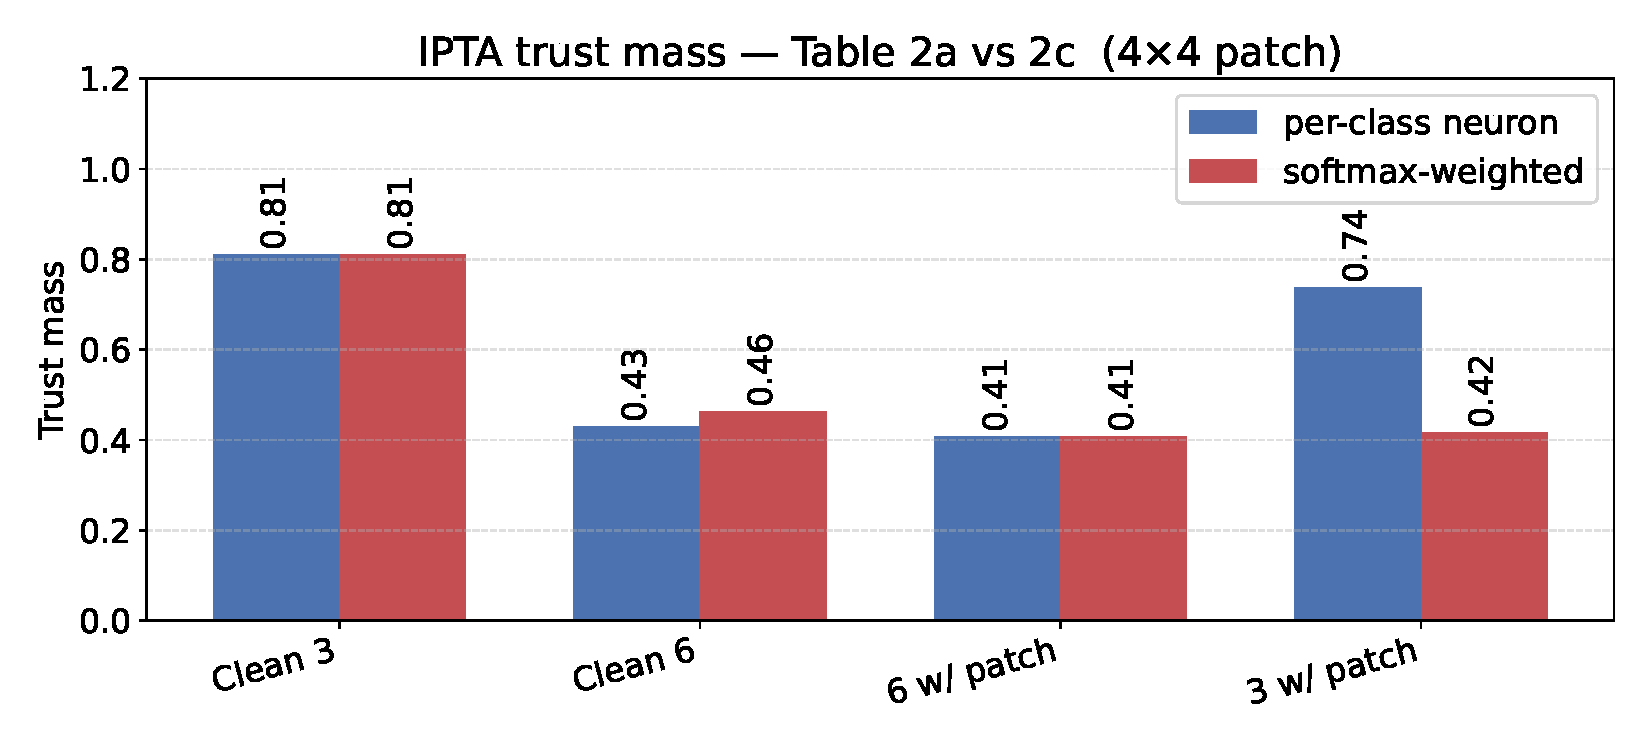
\includegraphics[width=0.8\linewidth]{latex/NN_Train_mnist_128_trust_trust_PathSize_4__ipta_trust_2a_vs_2c.pdf}
    \caption{IPTA trust mass comparison between per-class neuron and softmax-weighted aggregation ($\sum_i p_i t_i$) for the \ac{NN} trained on the poisoned dataset with patch size $4 \times 4$. The softmax-weighted aggregation weights each output neuron's trust mass by the model's predicted probability, producing a ranking that better reflects the reliability of the final decision rather than the inference path alone.}
    \label{fig:mnistpoisipta2}
\end{figure}



\section{Summary \& Conclusions}
\label{sec:patas-tp-conclusion}


This chapter presented \ac{PaTAS-TP}, a framework for propagating trust through
\acp{NN} in parallel with standard computation. The trust assessments stabilise
alongside model training in the sense of \cref{thm:convergence}, respect the
symmetry and invariance properties of \cref{sec:ptassyminv}, and respond to the
trust profiles assigned to the data in the four experimental settings. The
comparative evaluation makes the framework's value attributable rather than
aggregate, and the attribution is not flattering to propagation alone. The
detection of inputs that violate the training distribution is carried by the
input-side conformity opinions: on their own they reach AUROC $1.000$ on
\ac{OOD} detection from MNIST to Fashion-MNIST and on corruption detection on
MNIST, and $0.994$ on Fashion-MNIST, where the composed score reaches $0.975$,
$0.972$ and $0.835$. Propagation adds detection signal mainly under the
marginal-preserving translation ($0.781$ against $0.678$ for conformity alone),
and even there a feature-space nearest-neighbour detector is stronger ($0.801$).
The training-quality audit read from the trained trust state flags the presence
of label corruption at every non-zero flip rate, but at a saturated level
($0.682$ at every rate) that does not recover the corruption rate, whereas the
data-side disagreement baseline does. The contribution that no input-space or
output-only baseline expresses is therefore narrower than the aggregate numbers
suggest, and it is on the model side: the class-level localisation of
training-data poisoning, which separates the two flipped classes from every
clean class, distinguishes the label and trigger channels, and survives the
dead-unit and threshold checks. The evaluation also covers residual
convolutional networks at accuracies defensible for their domains ($99.3\%$
MNIST, $88.7\%$ Fashion-MNIST, $84.5\%$ CIFAR-10) through the activity-weighted
conv \ac{IPTA}; extending trust functions to transformer components and
normalization layers, and scaling the evaluation to top-tier training
pipelines, remain natural directions for future work.

A known limitation of the current design is that it structurally penalizes deeper
architectures. Each additional layer introduces an extra discounting step that
attenuates the trust signal, so deeper networks inherit less trust from their
inputs regardless of their predictive performance. The depth-normalized
aggregation introduced in \cref{sec:tp_arch_ovvw} compensates for the geometric
component of this decay and makes trust values comparable across depths, and it is
used alongside the raw aggregate in the audit of Experiment~4; a fully
depth-invariant formulation of the propagation itself, rather than a corrected
readout, remains future work. Two further limitations surfaced by the comparative
evaluation deserve explicit mention. First, the trust functions combine opinions
independently of weight and activation magnitudes: trust deliberately tracks the
provenance and reliability of the quantities entering a computation rather than
their functional influence, so an input the network effectively ignores can still
contribute to the output opinion. Partial influence-aware steps exist, the
softmax-weighted aggregation of Experiment~3 and the activity-weighted conv
\ac{IPTA}, but fully magnitude-aware trust functions remain open. Second, the
conformity-based input opinions detect support violations, not support subsets;
the subset-direction \ac{OOD} failure is predicted by the a-priori diagnostics,
and fusing a covariance- or neighborhood-based detector into the input opinion
through the same quantification is the natural \ac{SL} remedy.

A second limitation concerns the directional preservation of evidence established
in \cref{thm:infvac} and its Remark. While theoretically sound, this property implies that \ac{PaTAS-TP} cannot generate a non-zero distrust mass at the output when the input carries no distrust, that is, when $d_x = 0$, even if the model parameters are highly unreliable. In other words, parameter unreliability manifests as increased uncertainty rather than explicit distrust in the output opinion. This is a genuine
restriction in safety-critical settings where a positive distrust signal would be
more actionable than a high uncertainty mass. Every experiment of this chapter that feeds a fully trusted input therefore
reports $d = 0$ by construction, and the split between belief and uncertainty is
the only informative quantity there; this is stated together with the other
expressiveness limit in \cref{sec:dnn_trust}. Relaxing this constraint, for
instance by allowing parameter distrust to directly contribute a distrust component
to the output, is another avenue for future work.

Finally, the gradient-counting procedure used in \textsc{NodeTrust} fixes the
uncertainty component of the resulting binomial opinion based on the number of
input neurons, which may not be optimal in all cases. Adaptive quantification
schemes, as well as richer initialisation strategies for
$T_{n_i \mid \overline{y_\text{batch}}}$ beyond the vacuous opinion, are further
directions for improving the framework.









\chapter{CalibNN-SL: Method for Neural Network Calibration Quantification}
\label{chap:bb}
\todo[inline]{Estimated Nb Pages: 11}
\todo[inline]{Distinguish between black box and white box should have been made before}
\todo[inline]{Here an example a black box approach }
\todo[inline]{show advantages and limitations at the end}
\\
\\

\todo[inline]{How to structure the paper sections}
% \paragraph{Summary:}
% \paragraph{Problem:}
% \paragraph{Gap:}
% \paragraph{Method/Solution:}
% \paragraph{Findings:}
% \paragraph{Results:}
% \paragraph{Contribution:}
% \paragraph{Limitations:}
% \paragraph{Author Contribution:}
% \paragraph{Copyright Note: }
\paragraph{Summary (Introduction)}
\textbf{Purpose:} \\
To recap the context from previous chapters and highlight the key contributions of the current chapter.

\vspace{0.5em}
\textbf{It introduces:}
\begin{itemize}
    \item The gap in formal definitions
    \item The need to define "system adaptation" before "self-adaptive systems"
    \item The role of the MAPE-K model
    \item The proposed logical architecture
\end{itemize}

\vspace{0.5em}
\textbf{Use in your thesis:} \\
Begin each chapter with a brief overview of what was previously discussed and what this chapter contributes. This helps situate the reader.

%---------------------------------------------------------------
\paragraph{Problem Statement}
\textbf{Purpose:} \\
To clearly define the research problem(s) addressed in the chapter.

\vspace{0.5em}
\textbf{Problems include:}
\begin{itemize}
    \item Lack of clear definitions
    \item Conceptual confusion in terminology
    \item MAPE-K not differentiating between self-* systems
\end{itemize}

\vspace{0.5em}
\textbf{Use in your thesis:} \\
Clearly state the research gap and why it matters. This motivates your work and justifies your contribution.

%---------------------------------------------------------------
\paragraph{Gap Analysis}
\textbf{Purpose:} \\
To articulate what is missing in the current literature.

\vspace{0.5em}
\textbf{Identified gaps:}
\begin{itemize}
    \item Absence of a precise definition of "system adaptation"
    \item Lack of architectural blueprints
    \item Incomplete understanding of the adaptation process
\end{itemize}

\vspace{0.5em}
\textbf{Use in your thesis:} \\
Include a dedicated paragraph showing what others haven’t done yet, supported by citations. It strengthens the argument that your work is necessary.

%---------------------------------------------------------------
\paragraph{Method / Solution}
\textbf{Purpose:} \\
To describe what you are doing to solve the problem.

\vspace{0.5em}
\textbf{Proposed solution:}
\begin{itemize}
    \item Formal definition of system adaptation
    \item A logical architecture for CPSs
    \item A framework to bridge theory and implementation
\end{itemize}

\vspace{0.5em}
\textbf{Use in your thesis:} \\
Explain your proposed approach, framework, or method. Be specific and connect it to the identified problem.

%---------------------------------------------------------------
\paragraph{Findings / Key Questions for Framing}
\textbf{Purpose:} \\
To explain the foundational questions needed to define and analyze adaptivity.

\vspace{0.5em}
\textbf{Key framing questions:}
\begin{itemize}
    \item What is the function?
    \item What goals and context?
    \item What time scale and metrics?
\end{itemize}

\vspace{0.5em}
\textbf{Use in your thesis:} \\
Present any core framing questions or theoretical underpinnings that your method builds upon or introduces.

%---------------------------------------------------------------
\paragraph{Results}
\textbf{Purpose:} \\
To summarize the concrete results and contributions.

\vspace{0.5em}
\textbf{Your results might include:}
\begin{itemize}
    \item Validation of the formal definition
    \item Simulation setup and evaluation tools
    \item Generalizability of the Quality Function
\end{itemize}

\vspace{0.5em}
\textbf{Use in your thesis:} \\
Summarize the main outcomes and how they support your claims. Include both theoretical and empirical results.

%---------------------------------------------------------------
\paragraph{Contributions}
\textbf{Purpose:} \\
To make explicit what you contributed in this chapter.

\vspace{0.5em}
\textbf{Contributions include:}
\begin{itemize}
    \item Formalism
    \item Logical architecture
    \item Evaluation framework
    \item Metric for adaptation (Quality Function)
\end{itemize}

\vspace{0.5em}
\textbf{Use in your thesis:} \\
Have a clearly labeled paragraph listing your contributions. This helps reviewers and readers quickly see your impact.

%---------------------------------------------------------------
\paragraph{Limitations}
\textbf{Purpose:} \\
To acknowledge what your work doesn’t solve.

\vspace{0.5em}
\textbf{Limitations include:}
\begin{itemize}
    \item Ambiguities in the definition
    \item Partial observability in real CPSs
    \item Limitations of implementation
\end{itemize}

\vspace{0.5em}
\textbf{Use in your thesis:} \\
Be honest about limitations. This shows critical thinking and opens the door for future research.

%---------------------------------------------------------------
\paragraph{Author Contributions (optional)}
\textbf{Purpose:} \\
To credit each co-author for their role in collaborative work (common in paper-based theses).

\vspace{0.5em}
\textbf{Use in your thesis:} \\
Include if you are using published papers or co-authored chapters. This adds transparency.

\begin{itemize}
    \item \textbf{Author A}: Conceptual design, theoretical model.
    \item \textbf{Author B}: Implementation, validation.
    \item \textbf{Author C}: Experiments and analysis.
\end{itemize}

%---------------------------------------------------------------
\paragraph{Copyright Note (if applicable)}
\textbf{Purpose:} \\
To justify the inclusion of a reprinted article and show compliance with publisher rights.

\vspace{0.5em}
\textbf{Use in your thesis:} \\
Include if you are reprinting published articles. Follow your university’s thesis format.

\vspace{0.5em}
This chapter is based on the following published article: \\
\textit{Author names}, \textit{Paper title}, \textit{Journal Name}, \textbf{Volume}, Pages (Year). \\
DOI: \url{https://doi.org/xxxxxxx}. Reprinted with permission from the publisher.

% \todo[inline]{Example}

% \paragraph{Summary / Introduction}
% % Briefly summarize the previous chapter and introduce the content of this chapter.
% In this chapter, we build upon the findings from Chapter X and address two key challenges related to [...]. First, we tackle the lack of a formal definition of [...], and second, we propose an architectural framework for [...].

% \paragraph{Problem Statement}
% % State the main problems you aim to solve.
% Despite significant progress in [...], the engineering of [...] remains challenging. The absence of precise terminology and formal models hampers the development and evaluation of [...].

% \paragraph{Gap Analysis / Motivation}
% % Analyze the missing parts in the current literature.
% Existing literature proposes several models and frameworks for [...]; however, a precise, comprehensive, and widely accepted definition of [...] is still lacking. Additionally, architectural blueprints that support [...] in dynamic and uncertain contexts are rare.

% \paragraph{Proposed Method / Theoretical Contribution}
% % Present your solution or method.
% To address these issues, we propose a formal definition of [...], grounded in [...] theory. We also introduce a logical architecture for engineering [...] that supports [...].

% \paragraph{Theoretical Framework / Key Definitions}
% % Introduce the core definitions and theoretical framing.
% The foundation of our approach lies in defining the concept of [...]. We frame system adaptivity through the following key questions:
% \begin{itemize}
%     \item What is the system function (sf) considered adaptive?
%     \item What are the adaptation goals?
%     \item What context conditions trigger adaptation?
%     \item What time period is considered?
%     \item Under which convergence parameters is adaptivity assessed?
% \end{itemize}

% \paragraph{Results}
% % Describe what you achieved.
% We validate our approach through a model problem from the domain of [...]. We implemented a simulated system using [...], and evaluated the system adaptation using a metric referred to as the \textit{Quality Function}.

% \paragraph{Contributions}
% % Clearly state the novel contributions of this chapter.
% The main contributions of this chapter are:
% \begin{enumerate}
%     \item A formal definition of system adaptation.
%     \item A logical architecture for engineering [...]-adaptive systems.
%     \item A reusable evaluation framework with a Quality Function metric.
%     \item A differentiation between passive and active self-adaptation.
% \end{enumerate}

% \paragraph{Limitations}
% % Acknowledge what your work does not cover.
% While our theoretical contributions are validated, several limitations exist:
% \begin{itemize}
%     \item The definition of adaptation depends on partial observability.
%     \item Implementation only realizes passive self-adaptation.
%     \item Quality Function relies on full state observability, which may not generalize.
% \end{itemize}

% \paragraph*{Author Contributions (if applicable)}
% \textbf{Author 1}: Conceptualization, theoretical formalism, implementation.\\
% \textbf{Author 2}: Architecture design and review.\\
% \textbf{Author 3}: Evaluation framework and experiment execution.

% \paragraph*{Copyright Note (if applicable)}
% This chapter is based on a previously published article: \\
% \textit{Author Names}, \textit{Title}, \textit{Journal}, \textbf{Volume}, Pages (Year). \\
% DOI: \url{https://doi.org/xxxxxx}. Reprinted with permission from Elsevier.


\chapter{Use Case: \acs{PaTAS} Applied to 5G Network Energy Management}
\label{chap:usecase}
\todo{rework c4, improve it}
\todo{split figure}
\todo{ackn that this is not the best model given the temporal nature of the problem an LSTM might be better}
\noindent
The previous chapters introduced the theoretical foundations and system architecture required to perform trust assessment in \ac{NN} systems. In particular, \cref{chap:ovl,chap:dataset-trust,chap:patas} introduced the \ac{PaTAS} architecture for parallel trust assessment through the whole \ac{NN} system pipeline. This chapter demonstrates how these contributions apply in practice through a concrete use case in 5G network energy management. The objective is not to introduce new theoretical contributions, but rather to illustrate how the proposed methodology can be applied to assess trustworthiness within a realistic \ac{ML} scenario. By instantiating the full trust assessment pipeline, from trust proposition definition to evidence collection, opinion quantification, and reasoning, we show how the framework can support practical decision-making regarding the trustworthiness of \ac{ML} systems.


\section{Introduction and Motivation}
\label{sec:intro}
5G network energy management is a trust-critical domain: decisions are automated, data arrives from heterogeneous hardware, and errors propagate directly into resource allocation. In this work, we evaluate \ac{PaTAS} using a real-world dataset from 5G network energy consumption monitoring\cite{netop_5g_energy_2026}. This scenario is particularly suited for evaluating \ac{PaTAS} because:
\begin{itemize}
    \item Data comes from heterogeneous infrastructure spanning more than 1,000 base stations with 12 different hardware types, creating natural variation in measurement reliability.
    \item Labels are derived via automated quantile binning, introducing systematic artifacts independent of measurement noise.
    \item Both features and labels carry inherent noise and uncertainty that must be explicitly modeled for trustworthy predictions.
    \item The task has direct practical significance: accurate energy modeling is essential for optimizing resource allocation in next-generation wireless networks.
\end{itemize}

Through this use case, we answer four questions:
\begin{enumerate}
    \item How should trust opinions be assigned to real-world data?
    \item How do trust opinions propagate through the network during training?
    \item Does the trust signal produced by \ac{PaTAS} reliably indicate prediction correctness under noise?
    \item How does \ac{PaTAS}-based per-prediction trust relate to a global calibration-trust assessment of the same model?
\end{enumerate}

The remainder of this chapter is organized as follows. \Cref{sec:dataset} describes the 5G energy dataset and experimental setup. \Cref{sec:trust_quantification} presents the trust quantification methodology for features and labels. \Cref{sec:trust_propagation} describes how trust opinions propagate through the network during training. \Cref{sec:noise_robustness} evaluates PaTAS as a confidence signal under noise. \Cref{sec:calibration_quantification} compares per-prediction trust with global calibration trust. \Cref{sec:discussion} discusses implications and limitations, and \Cref{sec:conclusion} concludes.


\section{Dataset and Experimental Setup}
\label{sec:dataset}
\subsection{The 5G Energy Dataset}
\label{sec:5g_dataset}

The 5G energy consumption dataset consists of operational measurements collected from a large-scale production network deployment over an 8-day period. It comprises measurements from more than 1,000 \acp{RRU} and \acp{AAU} spanning 12 distinct hardware product types, collected at hourly granularity. The dataset contains close to 100,000 base-station-level samples, providing substantial statistical power for evaluating trust quantification and propagation.


\subsubsection{Data Structure and Collection}
\label{sec:data_structure}

The dataset is organized into three coordinated CSV files that capture complementary aspects of network operation. \Cref{tab:data_files} summarizes these files.

\begin{table}[h]
\centering
\caption{5G Energy Dataset Files and Fields}
\label{tab:data_files}
\begin{tabular}{|l|p{3cm}|p{5cm}|}
\hline
\textbf{File} & \textbf{Content} & \textbf{Key Fields} \\
\hline
BSinfo.csv & Static base station and cell configuration & BS, CellName, RUType, Bandwidth, Frequency, Antennas, TXpower \\
\hline
CLstat.csv & Hourly cell-level operational status & Time, BS, CellName, Load, EnergySavingMode (1 to 6) \\
\hline
ECstat.csv & Hourly energy consumption per base station & Time, BS, Energy \\
\hline
\end{tabular}
\end{table}


\subsubsection{Feature Engineering and Label Definition}
\label{sec:features_labels}

Features are constructed through a multi-stage preprocessing pipeline. First, the three CSV files are joined on $(Time, BS, CellName)$. Cell-level measurements are aggregated to base station level by computing the mean of numerical features and the mode of categorical features. The resulting feature vector has 26 dimensions:

\begin{itemize}
    \item Load: 1 feature (cell utilization factor)
    \item Energy-saving mode: 6 features (ESMode1 to ESMode6, binary/ordinal indicators)
    \item Hardware characteristics: 5 features (Bandwidth, Frequency, Antennas, TXpower, NumCells)
    \item Equipment type: 14 features (one-hot encoding of 12 RUType variants plus 2 Modes)
\end{itemize}

All numerical features are standardized (mean approximately 0, standard deviation approximately 1) before use.

The target label is energy consumption discretized into three classes via quantile binning. Bin boundaries are computed independently for each base station and time window to reflect domain expectations about load-dependent energy usage. The three classes are Low (at or below the 33rd percentile), Medium (between 33rd and 66th percentile), and High (above the 66th percentile). Labels are created via automated quantile binning, which is computationally efficient but introduces natural label noise: measurement errors and temporal shifts cause static quantile boundaries to misalign with true energy classes. 
The impact of this natural noise is compounded by the controlled noise we 
introduce experimentally, as described in \Cref{sec:noise_injection}.

\subsection{Model Configuration}
\label{sec:model_config}

We train a 2-layer \ac{MLP} with architecture $26 \to 32 \to 3$ to learn the energy classification task. We deliberately choose a simple architecture for three reasons: (1) it balances model capacity with interpretability, allowing clear observation of trust phenomena without the confounding of deep feature hierarchies; (2) it aligns with prior work on \ac{PaTAS} \cite{patas_chapter}, which has focused on shallow networks to enable controlled analysis of trust propagation; and (3) simple models provide a conservative baseline for evaluating whether trust reasoning adds value even in the simplest case, with the expectation that deeper networks may show larger benefits.

All neurons use ReLU hidden activations and softmax output activation. Training uses stochastic gradient descent with a fixed learning rate of $0.05$ and batch size of 64 for 10 epochs. Batch normalization and dropout are not used, in order to maintain transparency in trust propagation and avoid confounding factors in our analysis.

Parameter trust opinions are initialized to the vacuous state $(b=0, d=0, u=1)$ in both layers, representing complete ignorance before training. The \ac{PaTAS} and \ac{NN} run as separate processes communicating over a local \acs{TCP} socket, enabling modular integration of trust reasoning without modifying the underlying \ac{NN}'s forward or backward pass.


\subsection{Noise Injection Strategy}
\label{sec:noise_injection}

To evaluate \ac{PaTAS} under realistic data quality variation, we inject controlled noise into both features and labels. Feature noise is injected per-sample: each training sample $i$ independently draws its own noise level $\sigma_i$ from a uniform distribution:

\[
\sigma_i \sim \text{Uniform}(0, \sigma_{\max}), \quad i = 1, 2, \ldots, n
\]

Feature noise for sample $i$ is then additive Gaussian:

\[
\tilde{X}_i = X_i + \epsilon_i, \quad \epsilon_i \sim \mathcal{N}(0, \sigma_i \cdot \text{std}(X))
\]

To simulate label noise at controlled levels, we corrupt a fraction $p$ of all training labels by randomly reassigning them to an incorrect class, chosen uniformly from the remaining two classes. This controlled corruption mimics realistic label noise sources such as automated binning failures or inconsistent annotations, while keeping $p$ known by construction so that it can be used directly to compute the label trust opinion We conduct each experiment $N_{\text{RUNS}} = 5$ times with independent random number generator seeds. Results are averaged to obtain stable mean and standard deviation estimates.

\subsection{Experimental Configurations and Baselines}
\label{sec:configs}

We compare two configurations, summarized in \Cref{tab:configs}.

\begin{table}[h]
\centering
\caption{Experimental configurations. Both configurations use the same underlying neural network and dataset; they differ only in whether trust opinions are computed and propagated in parallel.}
\label{tab:configs}
\begin{tabular}{|l|p{3.5cm}|p{3.5cm}|c|}
\hline
\textbf{Config} & \textbf{Feature trust at training} & \textbf{Label trust at training} & \textbf{Runs} \\
\hline
nn & None (baseline NN) & None & 5 \\
\hline
ptas-percal & Per-sample $\sigma_i$ calibration & flip probability $p$ & 5 \\
\hline
\end{tabular}
\end{table}

The \textbf{nn} baseline is a standard neural network without any trust reasoning. It establishes the underlying classification performance and serves as the reference for evaluating \ac{PaTAS}, which does not modify the \ac{NN}'s predictions but provides a complementary trust signal.

The \textbf{ptas-percal} configuration runs \ac{PaTAS} alongside the same \ac{NN} with per-sample heterogeneous trust. Each training sample $i$ has its trust opinion computed as $\text{feature\_noise\_to\_trust}(\sigma_i)$, with $\sigma_i$ drawn as described above. The \ac{PaTAS} looks up $\sigma_i$ by batch index on-the-fly, constructing heterogeneous trust matrices where each row carries distinct belief, disbelief, and uncertainty values. Label trust is computed from the flip probability $p$ via $\text{label\_noise\_to\_trust}(p)$.

\paragraph{Training versus evaluation trust opinions.}
During training, feature trust is heterogeneous (per-sample $\sigma_i$) to reflect the realistic situation where different samples have different reliability. During evaluation, we report \ac{PaTAS} as a function of a single $\sigma_{\text{rel}}$ value, computed by evaluating $\text{feature\_noise\_to\_trust}(\sigma_{\text{rel}})$ uniformly across test samples. This allows controlled comparison of PaTAS behavior under specific noise levels without confounding from per-sample variation. The training-time heterogeneity ensures the network has been exposed to a realistic mix of sample qualities; the evaluation-time uniformity isolates the effect of a given noise condition.


\subsection{Experiments, Training and Evaluation Protocol}
\label{sec:exp_axes}

We evaluate the system along two primary axes:

\begin{enumerate}
    \item \textbf{Feature noise:} $\sigma_{\text{rel}} \in \{0.0, 0.1, 0.3, 0.5\}$ with label flip probability $p = 0$.
    \item \textbf{Combined noise:} Selected pairs $(\sigma_{\text{rel}}, p) \in \{(0.1, 0.05), (0.3, 0.15), (0.5, 0.30)\}$.
\end{enumerate}

For each condition, both \textbf{nn} and \textbf{ptas-percal} are run five times. Reported results are means with standard deviations across runs. 

The pairing of feature and label noise levels is chosen to reflect realistic scenarios where data quality degrades on multiple dimensions simultaneously. At higher feature noise levels $\sigma_{rel}$, we pair correspondingly higher label flip rates $p$ to simulate the expectation that measurement degradation and labeling errors co-occur in production systems.

\paragraph{Training loop.} 
At each training step, the \ac{NN} sends batches of size 64 to the \ac{PaTAS} along with batch indices. The \ac{PaTAS}  retrieves the per-sample trust opinions for that batch and propagates them through the \acf{TNN} in parallel with the standard \ac{NN}'s forward and backward pass. After training, test-time \ac{PaTAS} opinions are computed on the held-out test set under each evaluation condition. We report:
\begin{itemize}
    \item Final test accuracy of the baseline \ac{NN}.
    \item Learning curves showing epoch-wise progression.
    \item \ac{PaTAS} opinion masses $(b, d, u)$ on the \ac{NN}'s predicted class, separated by whether the prediction is correct.
    \item Selective-prediction coverage and accuracy under \ac{PaTAS}-based and softmax-based filters.
\end{itemize}


\section{Trust Assessment: Assigning Opinions to Data}
\label{sec:trust_quantification}

We quantify trust opinions by mapping noise characteristics directly to binomial opinion components $(b, d, u)$ using two domain-specific functions: one for feature noise, one for label noise. This approach embeds the semantic distinction between random measurement variability and systematic labeling errors into the opinion structure itself.


\subsection{Feature Trust Quantification}
\label{sec:feature_trust_quantification}

We define the mapping from noise level to uncertainty as the noise-to-information ratio. Intuitively, a noisy measurement carries less information relative to the signal it is meant to convey. We formalize this by treating $\sigma_{\text{rel}}^2$ as the noise power and 1 as the unit signal power. Since $\sigma_{\text{rel}} < 1$ by construction (noise is always smaller than the signal after z-standardization), the raw ratio $\sigma_{\text{rel}}^2 / (1 + \sigma_{\text{rel}}^2)$ only reaches 0.5 at its maximum ($\sigma_{\text{rel}} = 1$), leaving the upper half of the uncertainty range $[0, 1]$ unreachable. We therefore apply a factor of 2 to rescale the mapping to the full $[0, 1]$ interval:

\begin{equation}
u = \frac{2\sigma_{\text{rel}}^2}{1 + \sigma_{\text{rel}}^2}
\label{eq:feature_u}
\end{equation}

This is consistent with our z-standardization of features in 
\Cref{sec:features_labels}: after standardization, the signal variance is 1 
by construction, making $\sigma_{\text{rel}}^2 / (1 + \sigma_{\text{rel}}^2)$ directly interpretable as the noise-to-signal ratio. 

The remaining mass $1 - u$ is distributed between belief and disbelief (Constant-Uncertainty Quantification in \cref{chap:Trust_method}). Positive and negative evidence are taken as:
\begin{equation}
r = 1 - \sigma_{\text{rel}}, \quad s = \sigma_{\text{rel}}
\end{equation}

and normalized by $\gamma = (1 - u) / (r + s) = 1 - u$, giving:

\begin{equation}
b = (1 - \sigma_{\text{rel}}) (1 - u), \quad d = \sigma_{\text{rel}} (1 - u).
\label{eq:feature_bd}
\end{equation}

The rescaled mapping satisfies three desirable properties:
\begin{itemize}
    \item \textbf{Boundary correctness}: at $\sigma_{\text{rel}} = 0$ (no noise), 
    $u = 0$, yielding the fully-trusted opinion $(1, 0, 0)$; at 
    $\sigma_{\text{rel}} = 1$ (noise power equals signal power), $u = 1$, 
    yielding the vacuous opinion $(0, 0, 1)$.
    \item \textbf{Monotonicity}: $u$ increases strictly with $\sigma_{\text{rel}}$, 
    ensuring that higher noise always produces more uncertainty.
    \item \textbf{Boundedness}: $u \in [0, 1]$ for all $\sigma_{\text{rel}} \in [0, 1]$, 
    guaranteeing a valid opinion at every noise level within the operating range.
\end{itemize}

Moreover, as measurement noise increases, uncertainty grows as the dominant component, while both belief and disbelief shift: belief decreases from 1 toward 0, and disbelief increases from 0 toward a maximum at $\sigma_{\text{rel}} = 0.5$ before both collapse as $u \to 1$. The net effect is uncertainty-dominant: for $\sigma_{\text{rel}} \leq 1$, uncertainty is always the largest single component, reflecting that noisy measurements reduce confidence without implying systematic deception.




\subsection{Label Trust Quantification}
\label{sec:label_trust_quantification}

Label noise from automated binning represents class-flipping errors, where a fraction $p$ of labels are systematically reassigned to the wrong class. Unlike random measurement noise, label flipping is a failure mode of the labeling process itself, producing a disbelief-dominant opinion.

We quantify label trust through a direct linear mapping of flip rate to disbelief:

\begin{equation}
b = 1 - p, \quad d = p, \quad u = 0.
\label{eq:label_bdu}
\end{equation}

At $p = 0$ (clean labels), the opinion is $(1, 0, 0)$ (fully trusted). As the flip rate increases, belief decreases linearly while disbelief rises symmetrically. At $p = 1.0$, the opinion becomes $(0, 1, 0)$, indicating that the labels are reliably wrong. 

The absence of uncertainty ($u = 0$) reflects a deliberate modeling choice grounded in the nature of label errors. Uncertainty in \ac{SL} represents \emph{vacuity}: genuine epistemic doubt about whether a proposition is true or false. Feature noise introduces vacuity because, even knowing $\sigma_{\text{rel}}$, we cannot determine whether any individual measurement is too high or too low, the error is random and unbiased, so it creates irreducible doubt about each specific value. Label flipping, by contrast, is deterministic in its effect: a flipped label is definitively wrong, not merely uncertain. Knowing $p$ tells us precisely what fraction of labels to disbelieve, with no residual ambiguity about their incorrectness. We therefore encode label noise as a clean partition between belief and disbelief: $b = 1 - p$ for the fraction of labels we trust to be correct, and $d = p$ for the fraction we know to be wrong, with $u = 0$ reflecting the absence of vacuity.


\paragraph{Comparison of Feature and Label Trust Quantification}
\label{sec:trust_comparison}

The two quantification functions embody distinct failure modes:

\begin{itemize}
    \item \textbf{Feature noise} (measurement uncertainty): Random, unbiased, hard to detect during training. Produces uncertainty-dominant opinions: high noise yields $(b \approx 0, d \approx 0, u \approx 1)$.
    \item \textbf{Label noise} (labeling errors): Systematic, deterministic in effect, encoded as a known flip rate. Produces disbelief-dominant opinions with zero uncertainty: high noise yields 
    $(b \approx 0, d \approx 1, u = 0)$.
\end{itemize}
This semantic distinction allows \ac{PaTAS} to reason differently about each source: measurement uncertainty increases overall epistemic doubt while preserving some confidence, whereas label errors produce concrete disbelief with no residual vacuity. \Cref{fig:trust_mapping} visualizes the resulting opinion components as a function of $\sigma_{\text{rel}}$ and $p$ respectively, confirming that the two mappings produce qualitatively distinct opinion profiles across the full range of noise levels used in our experiments.

\section{Trust Propagation: How Opinions Evolve During Training in \ac{PaTAS}}
\label{sec:trust_propagation}

The previous section described how trust opinions are assigned at the data level. This section describes how these opinions propagate through the \ac{NN} during training, producing trust opinions on the network's predictions. The mechanisms described here operationalize the Trust Propagation part of the \ac{PaTAS} framework introduced in \cref{chap:patas}: the use case instantiates the Trust Feedforward and Parameter-Trust Update modules on the 5G energy classification task.


% \subsection{Subjective Logic Operators in \ac{PaTAS}}
% \label{sec:sl_operators_recap}

Several \ac{SL} operators drive trust propagation in \ac{PaTAS}: \emph{trust discounting} and \emph{belief fusion} for forward propagation, and \emph{deduction} combined with \emph{belief fusion} for the trust update applied during backpropagation.


\subsection{Trust Discounting and Fusion for Forward Propagation}
\label{sec:discounting_forward}

When trust opinions flow from inputs through the network, they encounter weight opinions $\omega_{\theta_{i,j}^{(l)}}$ that represent the learned trust in each parameter $\theta_{i,j}^{(l)}$, the weight connecting neuron $j$ in layer $l-1$ to neuron $i$ in layer $l$. Trust propagation through a single Trust Node mirrors the structure of the corresponding neuron: where the neuron computes a weighted sum followed by an activation, the Trust Node replaces multiplication by discounting and summation by fusion.

Concretely, for each neuron $i$ in layer $l$, the Trust Function computes:

\begin{equation}
T_{z^{(l)}_i} = \bigvee_{j \in \mathcal{N}(i)} T_{x^{(l-1)}_j} \otimes T_{\theta^{(l)}_{i,j}}, 
\qquad 
T_{x^{(l+1)}_i} = T_{\varphi^{(l)}}\!\left(T_{z^{(l)}_i}\right)
\label{eq:trust_function}
\end{equation}

where $\otimes$ is the trust discounting operator, $\bigvee$ denotes the fusion operator aggregating contributions from all predecessors $\mathcal{N}(i)$, and $T_{\varphi^{(l)}}$ is the trust-equivalent of the activation function, set to the identity in this work since we use \ac{ReLU} activations~(\cref{chap:patas}).

The two operations have complementary roles:

\begin{itemize}
    \item \textbf{Trust discounting} ($\otimes$) models the dependency of a downstream component on an upstream one. An input opinion $T_{x_j}$ discounted by parameter trust $T_{\theta_{i,j}}$ yields a refined opinion reflecting that the reliability of the parameter limits how much of the input's trustworthiness can be passed on. If the parameter is fully trusted $(1,0,0)$, the input opinion is passed through unchanged; if the parameter is vacuous $(0,0,1)$, the discounted opinion collapses to vacuous regardless of the input.
    \item \textbf{Belief fusion} ($\bigvee$) aggregates independent contributions from multiple predecessors into a single opinion. Since each input feature $x_j$ provides independent evidence for the neuron's output, cumulative fusion is the appropriate operator: it accumulates evidence across sources, reducing uncertainty as more sources agree.
\end{itemize}

This two-step process propagates layer by layer from inputs to outputs, with weight opinions $\omega_\theta$ initialized to the vacuous state $(0, 0, 1)$ before training begins. The feedforward procedure is summarized in Algorithm~5 of \cref{chap:patas}.


\subsection{Deduction and Fusion for Parameter Updates}
\label{sec:deduction_fusion}

During backpropagation, gradient information is converted into trust evidence to update the weight opinions $\omega_{\theta_{i,j}^{(l)}}$. The update mirrors the structure of standard gradient descent (\cref{eq:gd1} in \cref{chap:patas}): just as the gradient $\partial \mathcal{L}/\partial \theta_{i,j}^{(l)}$ factors into an error term $\delta_i^{(l)}$ and an input activation $x_j^{(l-1)}$, the Parameter-Trust Update incorporates gradient evidence, label trust, and input feature trust as analogous sources of evidence. The procedure, detailed in Algorithm~6 of \cref{chap:patas}, proceeds in three stages per neuron:

\begin{enumerate}
    \item \textbf{Gradient-to-opinion conversion.} For neuron $n_i^{(l)}$, the gradients $\{g_{i,j}^{(l)}\}$ of its incoming weights are classified by magnitude against a sensitivity threshold $\epsilon = 0.05$: weights with $|g_{i,j}^{(l)}| < \epsilon$ contribute positive evidence $r$ (the gradient is small, indicating the parameter is near a reliable optimum), and weights with $|g_{i,j}^{(l)}| \geq \epsilon$ contribute negative evidence $s$. These counts are mapped to a binomial opinion $T_{n_i \mid y_{\text{batch}}}$ via \ac{BPQ}.

    \item \textbf{Deduction against label trust.} The gradient opinion is conditioned on the batch label trust $T_{y_{\text{batch}}}$ using the inferential deduction operator $\circledast$, yielding a deduced neuron trust $T_{n_i \| Y_{\text{batch}}}$. This step accounts for the fact that gradient signals are only meaningful insofar as the labels driving them are themselves trustworthy: a strong gradient driven by a mislabeled sample should not increase parameter trust.

    \item \textbf{Revision and adjustment of parameter trust.} The weight opinion $T_{\theta_{i,j}^{(l)}}$ is first revised using $T_{n_i \| Y_{\text{batch}}}$, then adjusted by the joint influence of input feature trust $T_{x_j^{(l-1)}}$ and label trust $T_{y_{\text{batch}}}$. This adjustment reflects Eq.~(7.6) of \cref{chap:patas}: parameter updates depend jointly on gradient signals, input activations, and label quality, so parameter trust must account for all three.
\end{enumerate}

The net effect is that parameter trust accumulates evidence across mini-batches via cumulative fusion, converging as training progresses. Under clean conditions, weight opinions converge toward high belief; under noisy inputs or labels, trust accumulation is modulated by the degraded input and label opinions, leaving elevated uncertainty or disbelief in the affected weights.


\subsection{Implementation Details}
\label{sec:impl_details_propagation}

The \ac{PaTAS} server and \ac{NN} client communicate via \acs{TCP} sockets, realizing the \ac{NN} Interface described in \cref{chap:patas}. The interaction at each training step proceeds as follows:

\begin{itemize}
    \item The client sends a \texttt{TRAINING\_FEEDFORWARD} message containing the current batch indices.
    \item The \ac{PaTAS} server retrieves the per-sample noise levels $\sigma_i$ stored in \texttt{sigma\_arr}, constructs the heterogeneous input trust array $T_x$ (one opinion per sample per feature), and applies the Trust Feedforward to propagate trust through both layers of the \ac{TNN}, storing intermediate trust scores for use in the update step.
    \item After the client computes gradients, it sends a \texttt{TRAINING\_BACKPROPAGATION} message containing $\delta_W$, $\delta_b$, and the true labels $y$.
    \item The \ac{PaTAS} server constructs the batch label trust opinion $T_{y_{\text{batch}}}$ via $\text{label\_noise\_to\_trust}(p)$, runs the Parameter-Trust Update (\cref{alg:trustupdate} in \cref{chap:patas}) to revise $\omega_\theta$ for each layer, and sends an acknowledgement.
\end{itemize}

By design, the trust feedforward and parameter update are fully independent of the standard \ac{NN} computation: the network's weights, gradients, and predictions are unaffected by the parallel trust reasoning. \ac{PaTAS} operates as a confidence signal, not as a regularizer or a modifier of learning dynamics.

\section{Noise Robustness: \ac{PaTAS} as a Confidence Signal Under Data Quality Variation}
\label{sec:noise_robustness}

This section evaluates \ac{PaTAS} in its intended role: providing an interpretable trust opinion that signals the reliability of \ac{NN} predictions. Rather than asking whether \ac{PaTAS} improves classification accuracy (by design, it does not modify the \ac{NN}'s predictions), we ask: \emph{can the trust opinion produced by \ac{PaTAS} be used to selectively improve accuracy on retained predictions?} If the trust signal discriminates reliably between correct and incorrect predictions, it can support downstream decision-making by filtering out low-confidence samples and improving accuracy on the subset that passes the filter.


\subsection{Baseline Neural Network Performance}
\label{sec:baseline_nn}

We first establish baseline \ac{NN} performance under our two experimental axes. \Cref{fig:feature_noise_accuracy} shows test accuracy as feature noise $\sigma_{\text{rel}}$ increases from 0 to 0.5, and \Cref{fig:combined_accuracy} reports performance under combined feature and label noise.

\begin{figure}[h]
\centering
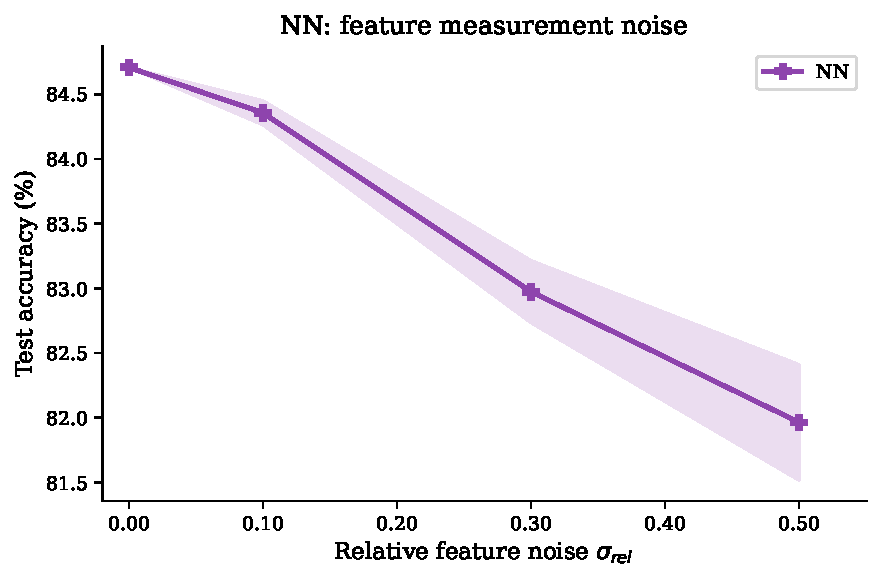
\includegraphics[width=0.7\textwidth]{img/usecase/feature_noise_accuracy.pdf}
\caption{Baseline \ac{NN} test accuracy as a function of relative feature noise $\sigma_{\text{rel}}$. Accuracy degrades monotonically from 84.7\% at $\sigma_{\text{rel}} = 0$ to 82.0\% at $\sigma_{\text{rel}} = 0.5$.}
\label{fig:feature_noise_accuracy}
\end{figure}

\begin{figure}[h]
\centering
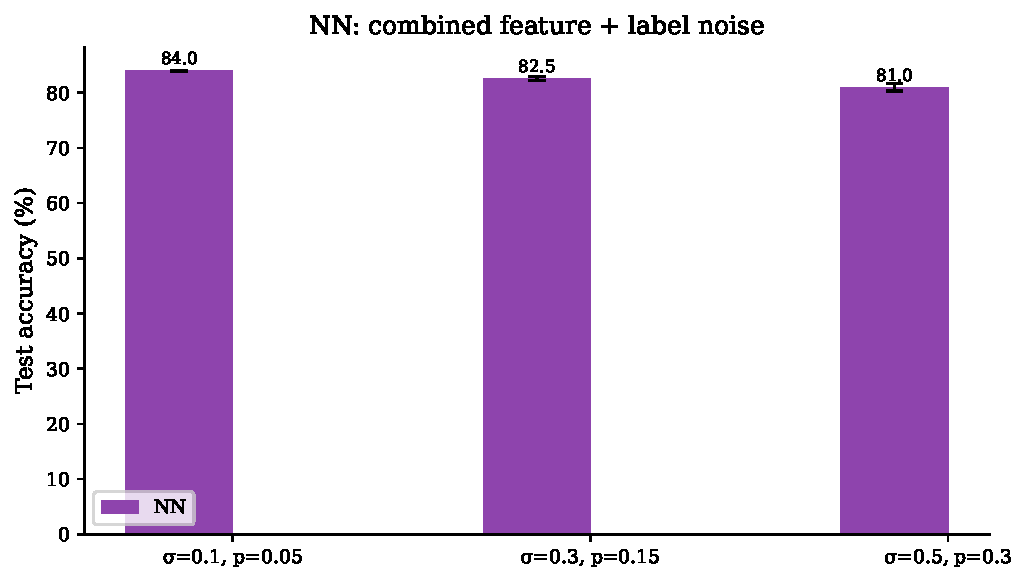
\includegraphics[width=0.7\textwidth]{img/usecase/combined_accuracy.pdf}
\caption{Baseline \ac{NN} test accuracy under combined feature and label noise. Accuracy degrades from 84.0\% at $(\sigma, p) = (0.1, 0.05)$ to 81.0\% at $(\sigma, p) = (0.5, 0.30)$.}
\label{fig:combined_accuracy}
\end{figure}

The \ac{NN} exhibits graceful degradation: accuracy decreases steadily but does not collapse, with a loss of 2.7 percentage points across the full feature-noise range and 3.0 percentage points across the combined-noise range. \Cref{fig:learning_curves} shows the corresponding learning curves over 10 training epochs. Convergence is stable across all conditions, confirming that the noise levels explored do not destabilize gradient-based learning.

\begin{figure}[h]
\centering
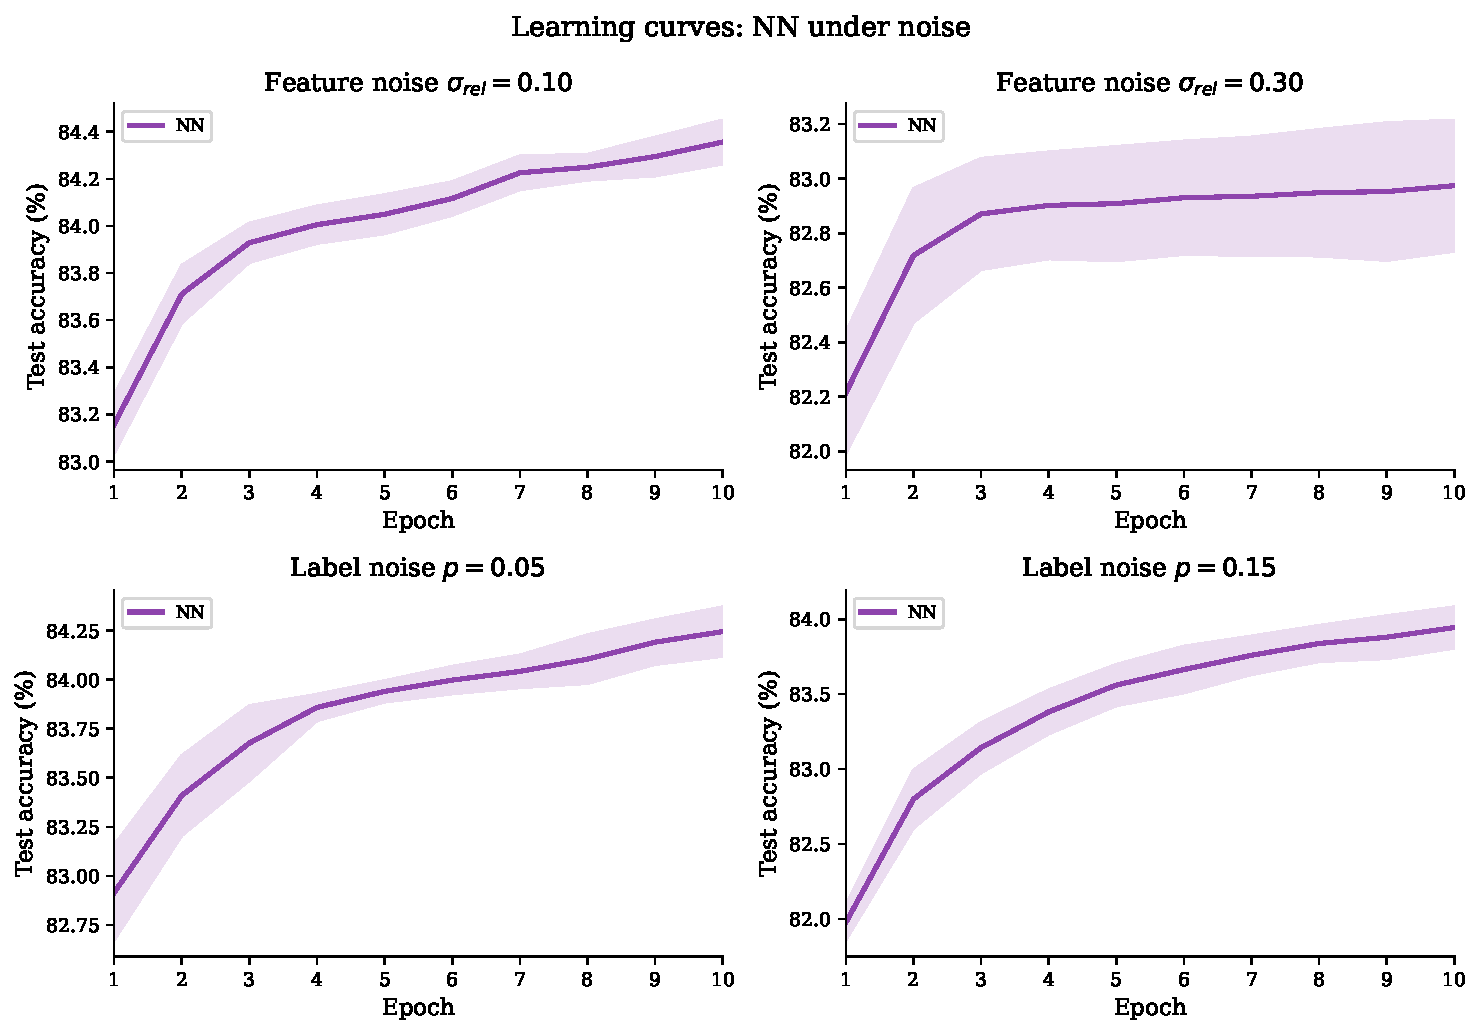
\includegraphics[width=\textwidth]{img/usecase/learning_curves.pdf}
\caption{Learning curves of the baseline \ac{NN} under feature noise ($\sigma_{\text{rel}} \in \{0.1, 0.3\}$, top) and label noise ($p \in \{0.05, 0.15\}$, bottom). All four conditions show monotonic convergence within 3 to 4 epochs, with final test accuracy between 82\% and 84\%.}
\label{fig:learning_curves}
\end{figure}


\subsection{Trust Opinion Mapping and Propagation Behavior}
\label{sec:trust_mapping_results}

Before evaluating the discriminative power of \ac{PaTAS} opinions, we verify that the calibration functions of \Cref{sec:trust_quantification} produce the expected mapping at the input layer. \Cref{fig:trust_mapping} visualizes the mapping for both noise sources, and \Cref{tab:trust-mapping} reports the numerical values used in our experiments.

\begin{figure}[h]
\centering
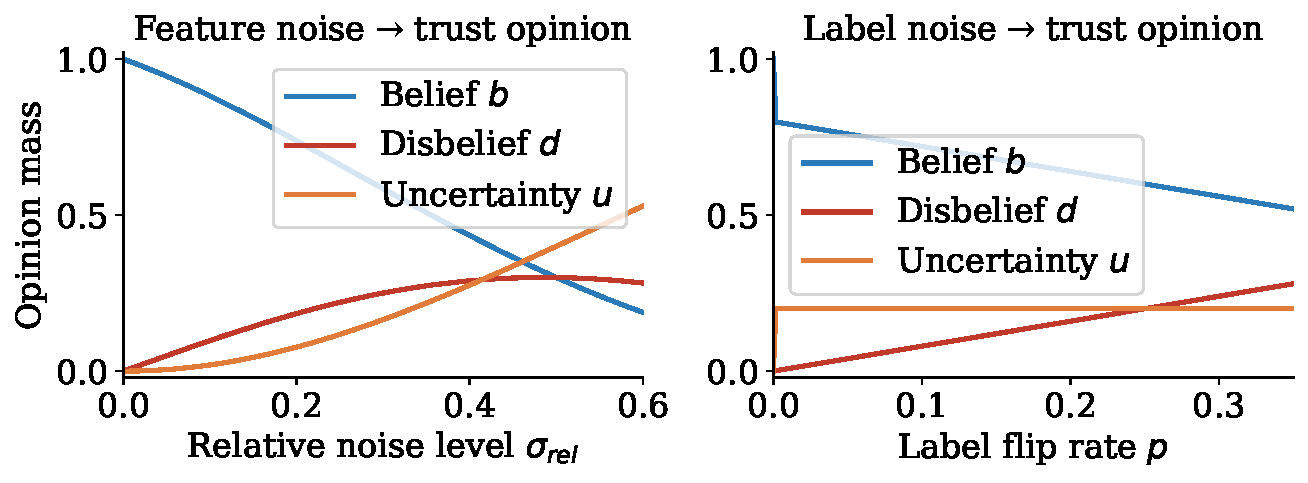
\includegraphics[width=\textwidth]{img/usecase/trust_mapping.pdf}
\caption{Trust opinion mapping at the input layer. Left: feature noise produces uncertainty-dominant opinions where $u$ grows with $\sigma_{\text{rel}}$ following \Cref{eq:feature_u}. Right: label noise produces disbelief-dominant opinions with $b = 1 - p$, $d = p$, and $u = 0$.}
\label{fig:trust_mapping}
\end{figure}

\input{img/usecase/trust_mapping}

The figure confirms the qualitatively distinct profiles designed into the two calibration functions. Feature noise produces increasing uncertainty, reaching $u = 0.40$ at $\sigma_{\text{rel}} = 0.5$ with correspondingly reduced belief and modest disbelief. Label noise produces a clean partition between belief and disbelief with zero residual uncertainty, consistent with the deterministic nature of the flip-rate model.

\paragraph{Propagation to the output layer.}
These input opinions are then propagated through the trained network for parameter trust quantification described in \Cref{sec:trust_propagation}. The benefit of this propagation is that the output opinion on each predicted class reflects both the quality of the input and the accumulated evidence about parameter reliability acquired during training. Because \ac{PaTAS} leaves the \ac{NN}'s predictions unchanged, the relevant evaluation question is not the magnitude of the output opinion in isolation, but whether it is informative about whether the prediction is correct. The following subsections answer this question directly.


\subsection{\ac{PaTAS} as a Discriminator of Correct Predictions}
\label{sec:patas_discriminator}

The central empirical question is whether \ac{PaTAS} opinions distinguish between correct and wrong \ac{NN} predictions. We compute the mean opinion components $(\bar{b}, \bar{d}, \bar{u})$ in the \ac{NN}'s predicted class, separately for samples where the prediction is correct and where it is wrong. A useful confidence signal should exhibit three simultaneous patterns:

\begin{itemize}
    \item Higher belief on correct predictions: $\bar{b}_c > \bar{b}_w$, i.e., $\Delta b > 0$.
    \item Lower uncertainty on correct predictions: $\bar{u}_c < \bar{u}_w$, i.e., $\Delta u < 0$.
    \item Lower disbelief on correct predictions: $\bar{d}_c < \bar{d}_w$, i.e., $\Delta d < 0$.
\end{itemize}

\Cref{fig:patas_effectiveness} visualizes these opinion masses, and \Cref{tab:ptas-effectiveness} reports the exact values.



% \begin{figure}[h]
% \centering
% 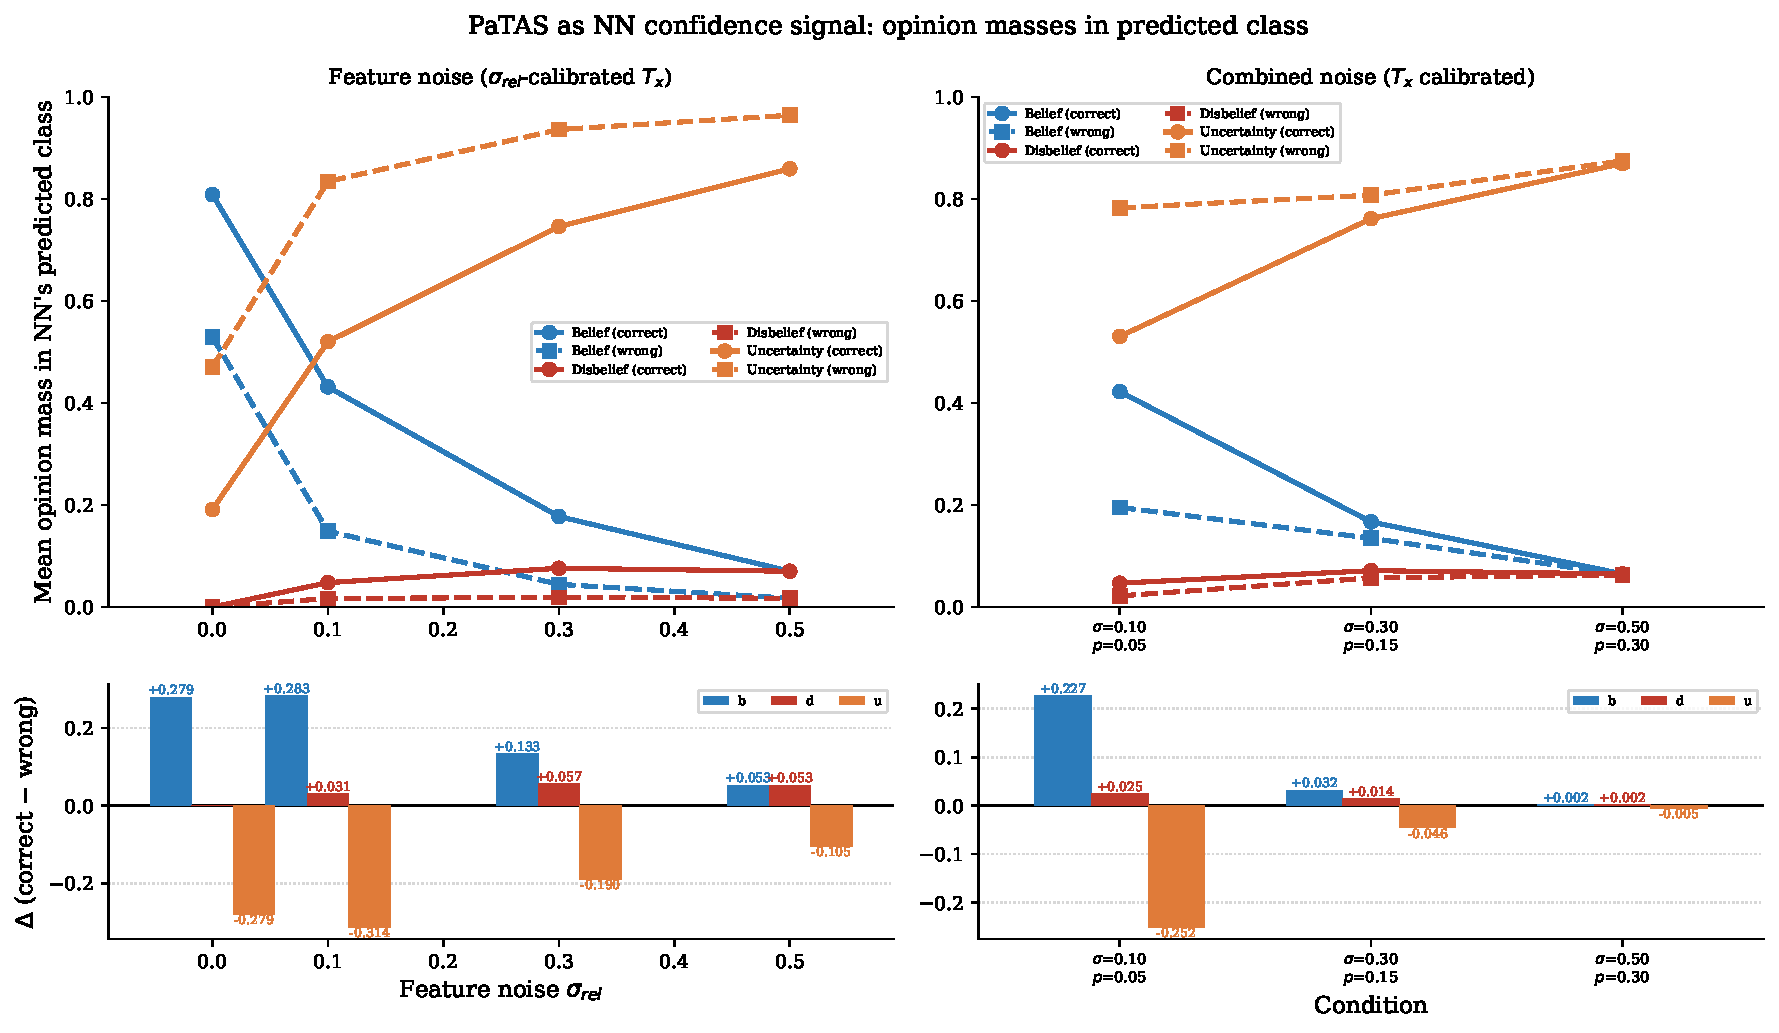
\includegraphics[width=\textwidth]{img/usecase/patas_effectiveness_test.pdf}
% \caption{\ac{PaTAS} opinion masses in the \ac{NN}'s predicted class. Top: mean opinion values for correctly-classified (solid lines, circles) versus mis-classified (dashed lines, squares) samples. Bottom: $\Delta = \text{correct} - \text{wrong}$, showing the discriminative gap per component. Left: feature noise. Right: combined noise.}
% \label{fig:patas_effectiveness}
% \end{figure}
\begin{figure}
    \centering
    \begin{subfigure}{0.7\textwidth}
        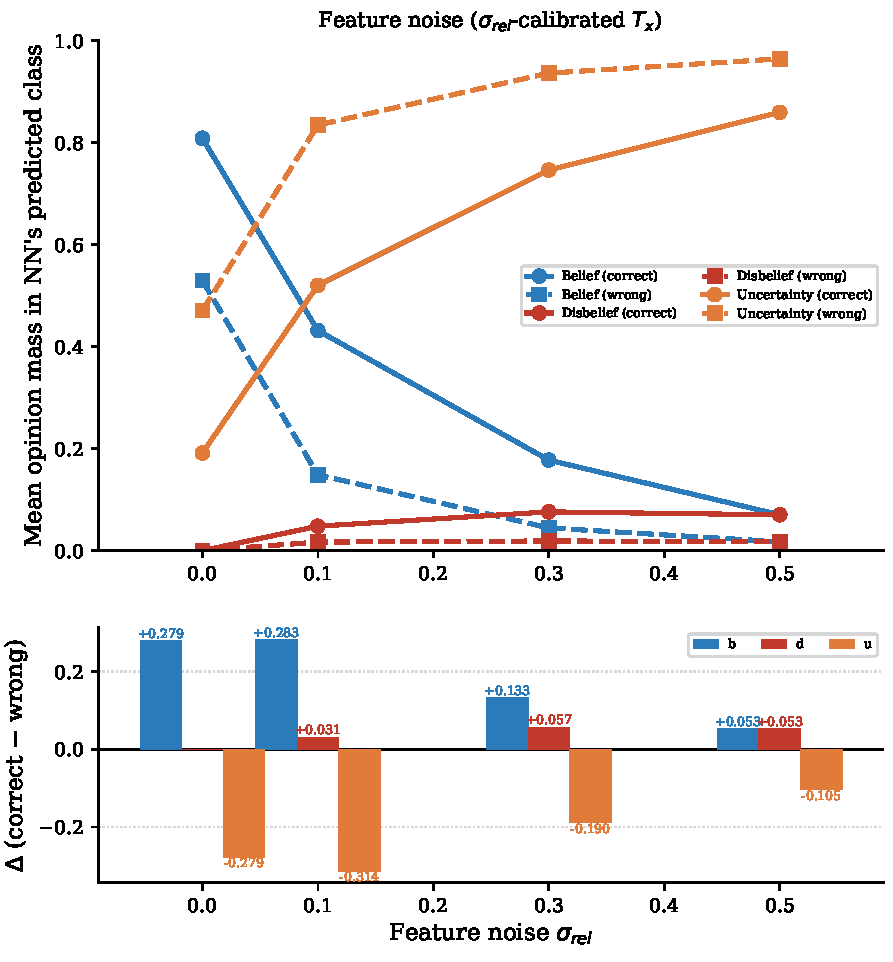
\includegraphics[width=\linewidth]{img/usecase/patas_effectiveness_test_cropped_1.pdf}
    \end{subfigure}
    \begin{subfigure}{0.7\textwidth}
        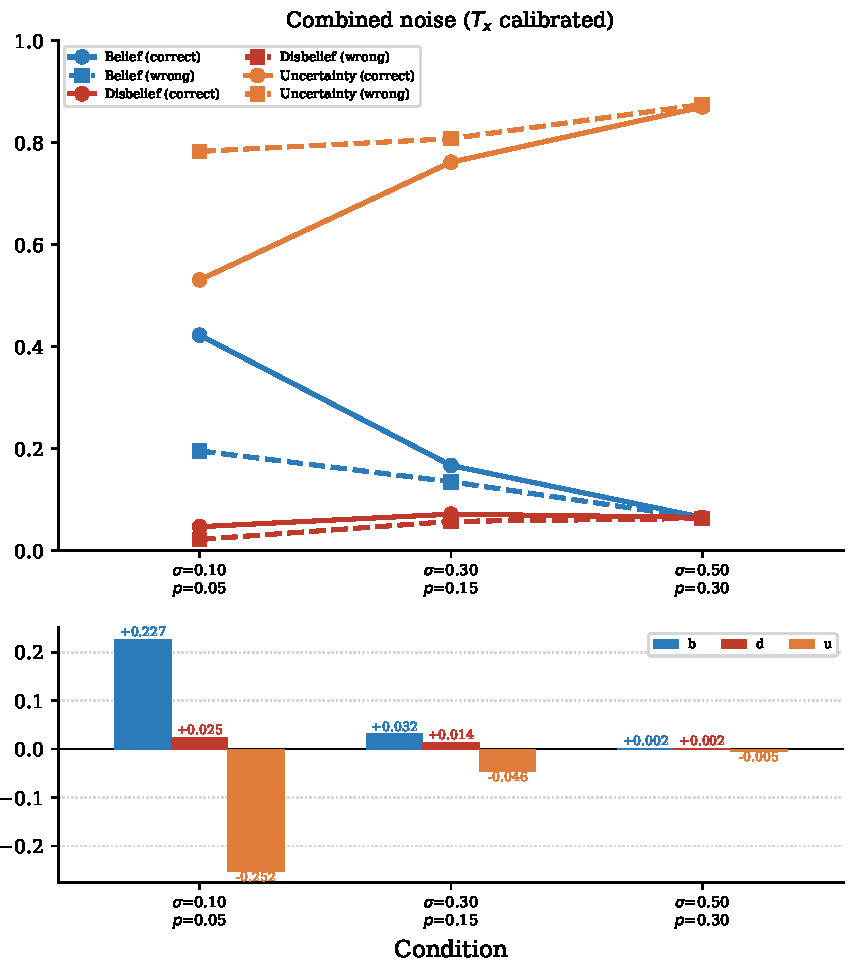
\includegraphics[width=\linewidth]{img/usecase/patas_effectiveness_test_cropped_2.pdf}
    \end{subfigure}
    \caption{\ac{PaTAS} opinion masses in the \ac{NN}'s predicted class. Top: mean opinion values for correctly-classified (solid lines, circles) versus mis-classified (dashed lines, squares) samples. Bottom: $\Delta = \text{correct} - \text{wrong}$, showing the discriminative gap per component. Left: feature noise. Right: combined noise.}
\label{fig:patas_effectiveness}
\end{figure}

\begin{table}[ht]
\centering
\caption{Mean \ac{PaTAS} opinion masses $(b, d, u)$ in the \ac{NN}'s predicted class, split by correct ($c$) vs.\ wrong ($w$) NN predictions. $\Delta = \text{correct} - \text{wrong}$; positive $\Delta b$ and negative $\Delta d$/$\Delta u$ indicate discriminability.}
\label{tab:ptas-effectiveness}
\begin{tabular}{lccccccccccc}
\toprule
Noise & $N_c$ & $N_w$ & $\bar{b}_c$ & $\bar{b}_w$ & $\Delta b$ & $\bar{d}_c$ & $\bar{d}_w$ & $\Delta d$ & $\bar{u}_c$ & $\bar{u}_w$ & $\Delta u$ \\
\hline
Feature noise \\
0.00 & 15692 & 2833 & 0.81 & 0.53 & +0.28 & 0.00 & -0.00 & +0.00 & 0.19 & 0.47 & -0.28 \\
0.10 & 15608 & 2917 & 0.43 & 0.15 & +0.28 & 0.05 & 0.02 & +0.03 & 0.52 & 0.83 & -0.31 \\
0.30 & 15407 & 3118 & 0.18 & 0.04 & +0.13 & 0.08 & 0.02 & +0.06 & 0.75 & 0.94 & -0.19\\
0.50 & 15265 & 3260 & 0.07 & 0.02 & +0.05 & 0.07 & 0.02 & +0.05 & 0.86 & 0.96 & -0.11 \\
\hline 
Combined noise \\
(0.10, 0.05) & 15527 & 2998 & 0.42 & 0.20 & +0.23 & 0.05 & 0.02 & +0.03 & 0.53 & 0.78 & -0.25 \\
(0.30, 0.15) & 15333 & 3192 & 0.17 & 0.14 & +0.03 & 0.07 & 0.06 & +0.01 & 0.76 & 0.81 & -0.05 \\
(0.50, 0.30) & 15061 & 3464 & 0.07 & 0.06 & +0.01 & 0.07 & 0.06 & +0.01 & 0.87 & 0.87 & -0.01 \\
\bottomrule
\end{tabular}
\end{table}

The results confirm clear discriminability under moderate noise:

\begin{itemize}
    \item At $\sigma_{\text{rel}} = 0.10$, \ac{PaTAS} belief on correct predictions ($\bar{b}_c = 0.43$) is nearly three times higher than on wrong predictions ($\bar{b}_w = 0.15$), yielding $\Delta b = +0.28$. Uncertainty exhibits the opposite pattern ($\Delta u = -0.31$), while disbelief remains low across both groups ($\bar{d} < 0.05$), confirming that \ac{PaTAS} treats feature noise as epistemic uncertainty rather than evidence of deception.
    \item At $\sigma_{\text{rel}} = 0.30$, discriminability persists but narrows ($\Delta b = +0.13$, $\Delta u = -0.19$), reflecting the degraded quality of the input trust signal as noise increases.
    \item At $\sigma_{\text{rel}} = 0.50$, both correct and wrong predictions receive similar opinions ($\Delta b = +0.05$). This is the expected behavior: when input quality approaches the maximum noise level, \ac{PaTAS} correctly signals that no prediction can be trusted, and the discriminative gap collapses accordingly.
\end{itemize}

Under combined noise, the discriminative gap at low corruption levels ($(\sigma, p) = (0.10, 0.05)$: $\Delta b = +0.23$) is comparable to the feature-only case, but narrows more sharply as both sources intensify together. At the most severe condition $(\sigma, p) = (0.50, 0.30)$, the gap is minimal ($\Delta b = +0.002$), with elevated uncertainty dominating both groups. This is consistent with the additive degradation of two independent noise sources simultaneously reducing the reliability of both input and label evidence available to the trust propagation mechanism.


\subsection{Selective Prediction Using \ac{PaTAS}}
\label{sec:selective_prediction}

A direct application of the discriminative capacity demonstrated above is selective prediction: rejecting predictions where the trust signal indicates low reliability, thereby improving accuracy on the retained subset. We evaluate two filters:

\begin{itemize}
    \item \textbf{\ac{PaTAS} filter} ($b > u$): retain samples where belief exceeds uncertainty in the predicted class, indicating that positive evidence for the prediction outweighs residual epistemic doubt.
    \item \textbf{Softmax filter} ($\text{softmax} > 0.5$): retain samples where the \ac{NN} softmax probability in the predicted class exceeds 0.5, the standard high-confidence threshold.
\end{itemize}

\Cref{tab:threshold-b-gt-d,tab:threshold-nn-0-50} compare the two filters across noise conditions.

\begin{table}[ht]
\centering
\caption{Selective prediction: \ac{PaTAS} belief-over-uncertainty filter ($b > u$). Coverage is the fraction of test samples where \ac{PaTAS} belief exceeds uncetainty in the \ac{NN}'s predicted class (net positive subjective evidence). Values are mean $\pm$ std over 5 independent runs.}
\label{tab:threshold-b-gt-d}
\begin{tabular}{lccc}
\toprule
Noise condition & Coverage (\%) & Accuracy on covered (\%) & Overall accuracy (\%) \\
\hline
\multicolumn{4}{l}{\textit{Feature noise ($T_x$ calibrated to $\sigma_{rel}$)}} \\
$\sigma_{rel}=0.10$ & 49.6 $\pm$ 16.5 & 89.38 $\pm$ 1.26 & 84.33 \\
\hline
\multicolumn{4}{l}{\textit{Combined noise ($T_x$ calibrated to $\sigma_{rel}$)}} \\
$\sigma=0.10,\,p=0.05$ & 32.7 $\pm$ 0.2 & 89.40 $\pm$ 2.23 & 84.00 \\
\bottomrule
\end{tabular}
\end{table}


\begin{table}[ht]
\centering
\caption{Selective prediction: NN softmax score threshold $\tau = 0.5$. Coverage is the fraction of test samples where the NN softmax probability in the predicted class exceeds $0.5$. Values are mean $\pm$ std over 5 independent runs.}
\label{tab:threshold-nn-0-50}
\begin{tabular}{lccc}
\toprule
Noise condition & Coverage (\%) & Accuracy on covered (\%) & Overall accuracy (\%) \\
\midrule
\multicolumn{4}{l}{\textit{Feature noise ($T_x$ calibrated to $\sigma_{rel}$)}} \\
$\sigma_{rel}=0.10$ & 97.9 $\pm$ 0.2 & 85.15 $\pm$ 0.09 & 84.36 \\
\midrule 
\multicolumn{4}{l}{\textit{Combined noise ($T_x$ calibrated to $\sigma_{rel}$)}} \\
$\sigma=0.10,\,p=0.05$ & 95.4 $\pm$ 0.3 & 85.73 $\pm$ 0.17 & 84.01 \\
\bottomrule
\end{tabular}
\end{table}


The \ac{PaTAS} filter is more selective and more accurate than the softmax filter across all evaluated conditions:

\begin{itemize}
    \item At $\sigma_{\text{rel}} = 0.10$, the \ac{PaTAS} filter retains 49.6\% of samples and achieves 89.4\% accuracy on that subset, a gain of 5.0 percentage points over the overall accuracy of 84.4\%. The softmax filter retains 97.9\% of samples but improves accuracy by only 0.8 percentage points (from 84.4\% to 85.2\%).
    \item Under combined noise at $(\sigma, p) = (0.10, 0.05)$, the \ac{PaTAS} filter achieves 89.4\% accuracy on 32.7\% coverage, while softmax achieves 85.7\% on 95.4\% coverage.
    \item The accuracy advantage of \ac{PaTAS} over softmax narrows as noise increases, consistent with the decreasing discriminative gap observed in \Cref{sec:patas_discriminator}.
\end{itemize}

The higher selectivity of the \ac{PaTAS} filter comes at the cost of coverage: at $\sigma_{\text{rel}} = 0.10$, half the samples are rejected. This trade-off is inherent to any threshold-based filter and depends on the deployment context. In high-stakes settings where incorrect predictions carry a high cost, the \ac{PaTAS} filter's precision is preferable. In settings where coverage matters, the two signals can be combined: samples passing the \ac{PaTAS} filter receive the trust-based accuracy guarantee, while remaining samples can be handled by a fallback strategy or flagged for human review.


\subsection{Summary of Robustness Findings}
\label{sec:robustness_summary}

Three conclusions follow from the empirical results:

\begin{enumerate}
    \item \ac{PaTAS} belief discriminates between correct and wrong predictions across all evaluated noise conditions. The discriminative gap $\Delta b$ ranges from $+0.28$ at low feature noise to $+0.05$ at high noise, with graceful degradation as data quality deteriorates.
    \item The nature of discrimination is consistent with the trust calibration design: feature noise produces uncertainty-driven separation ($\Delta u$ is the dominant signal), while combined noise produces a mixed signal with both uncertainty and belief components contributing.
    \item Used as a selective prediction filter, \ac{PaTAS} improves accuracy by 5.0 to 5.6 percentage points on retained samples, compared to 0.8 to 1.7 for softmax thresholding. The advantage derives from two complementary properties. First, the three-component opinion $(b, d, u)$ distinguishes vacuous predictions (high $u$, low $b$) from genuinely confident ones in a way that a single softmax probability cannot. Second, and more fundamentally, the trust opinion encodes explicit knowledge of data quality: the noise level $\sigma_i$ of each training sample is mapped to a calibrated opinion via $\text{feature\_noise\_to\_trust}(\sigma_i)$, and this quality signal propagates through the Trust Nodes Network alongside the standard forward pass. The output opinion therefore reflects not only the network's learned confidence but also how reliable the data used to form that confidence actually was. Softmax probabilities have no access to this provenance information and treat all predictions as equally grounded in the training data.
\end{enumerate}

\section{Calibration Quantification using Subjective Logic}
\label{sec:calibration_quantification}

The previous section evaluated PaTAS as a per-prediction confidence signal. We now turn to a complementary question: \emph{can we produce a single trust opinion that characterizes the trustworthiness of an entire trained model?} This is the calibration-trust problem, which we addressed in our earlier work using \acf{BPQ} with cumulative fusion across probability clusters (\cref{chap:bb}).

Unlike PaTAS, calibration quantification operates post-hoc on the predictions of an already-trained NN. The two methods are complementary: PaTAS provides per-sample trust during inference; calibration quantification provides a global trust opinion on the model itself. Evaluating both under the same noise conditions allows us to capture different aspects of trustworthiness.


\subsection{Methodology Recap}
\label{sec:calibration_methodology}

The calibration-trust algorithm (\cref{alg:1} in \cref{chap:bb}) computes a single binomial opinion $(b, d, u)$ on the trained NN as follows:
\begin{enumerate}
    \item \textbf{Clustering predictions.} The predicted probabilities for each class are partitioned into $M = 10$ bins over $[0, 1]$.
    \item \textbf{Per-cluster evidence.} For each bin $i$ with representative probability $\text{RP}_i$, positive evidence is the number of correct classifications $t_i$, and negative evidence is $|t_i - n_i \cdot \text{RP}_i|$, measuring the deviation between predicted and observed accuracy.
    \item \textbf{Per-cluster opinion.} A binomial opinion is computed via BPQ with uncertainty weight $W = 2$.
    \item \textbf{Cumulative fusion.} Cluster opinions are fused per class, then across classes, yielding a single calibration-trust opinion for the NN.
\end{enumerate}

This procedure quantifies how well the model's predicted probabilities align with its actual accuracy: a perfectly calibrated model receives an opinion approaching $(1, 0, 0)$, while a miscalibrated model shows elevated disbelief.


\subsection{Calibration Trust Across Noise Conditions}
\label{sec:calibration_results}
We compute calibration trust for the same trained networks evaluated in \Cref{sec:noise_robustness}, under feature noise, label noise, and combined noise. \Cref{fig:calibration_trust} visualizes the resulting opinion masses, and \Cref{tab:calibration-trust} reports the numerical values.

\begin{figure}[h]
\centering
% 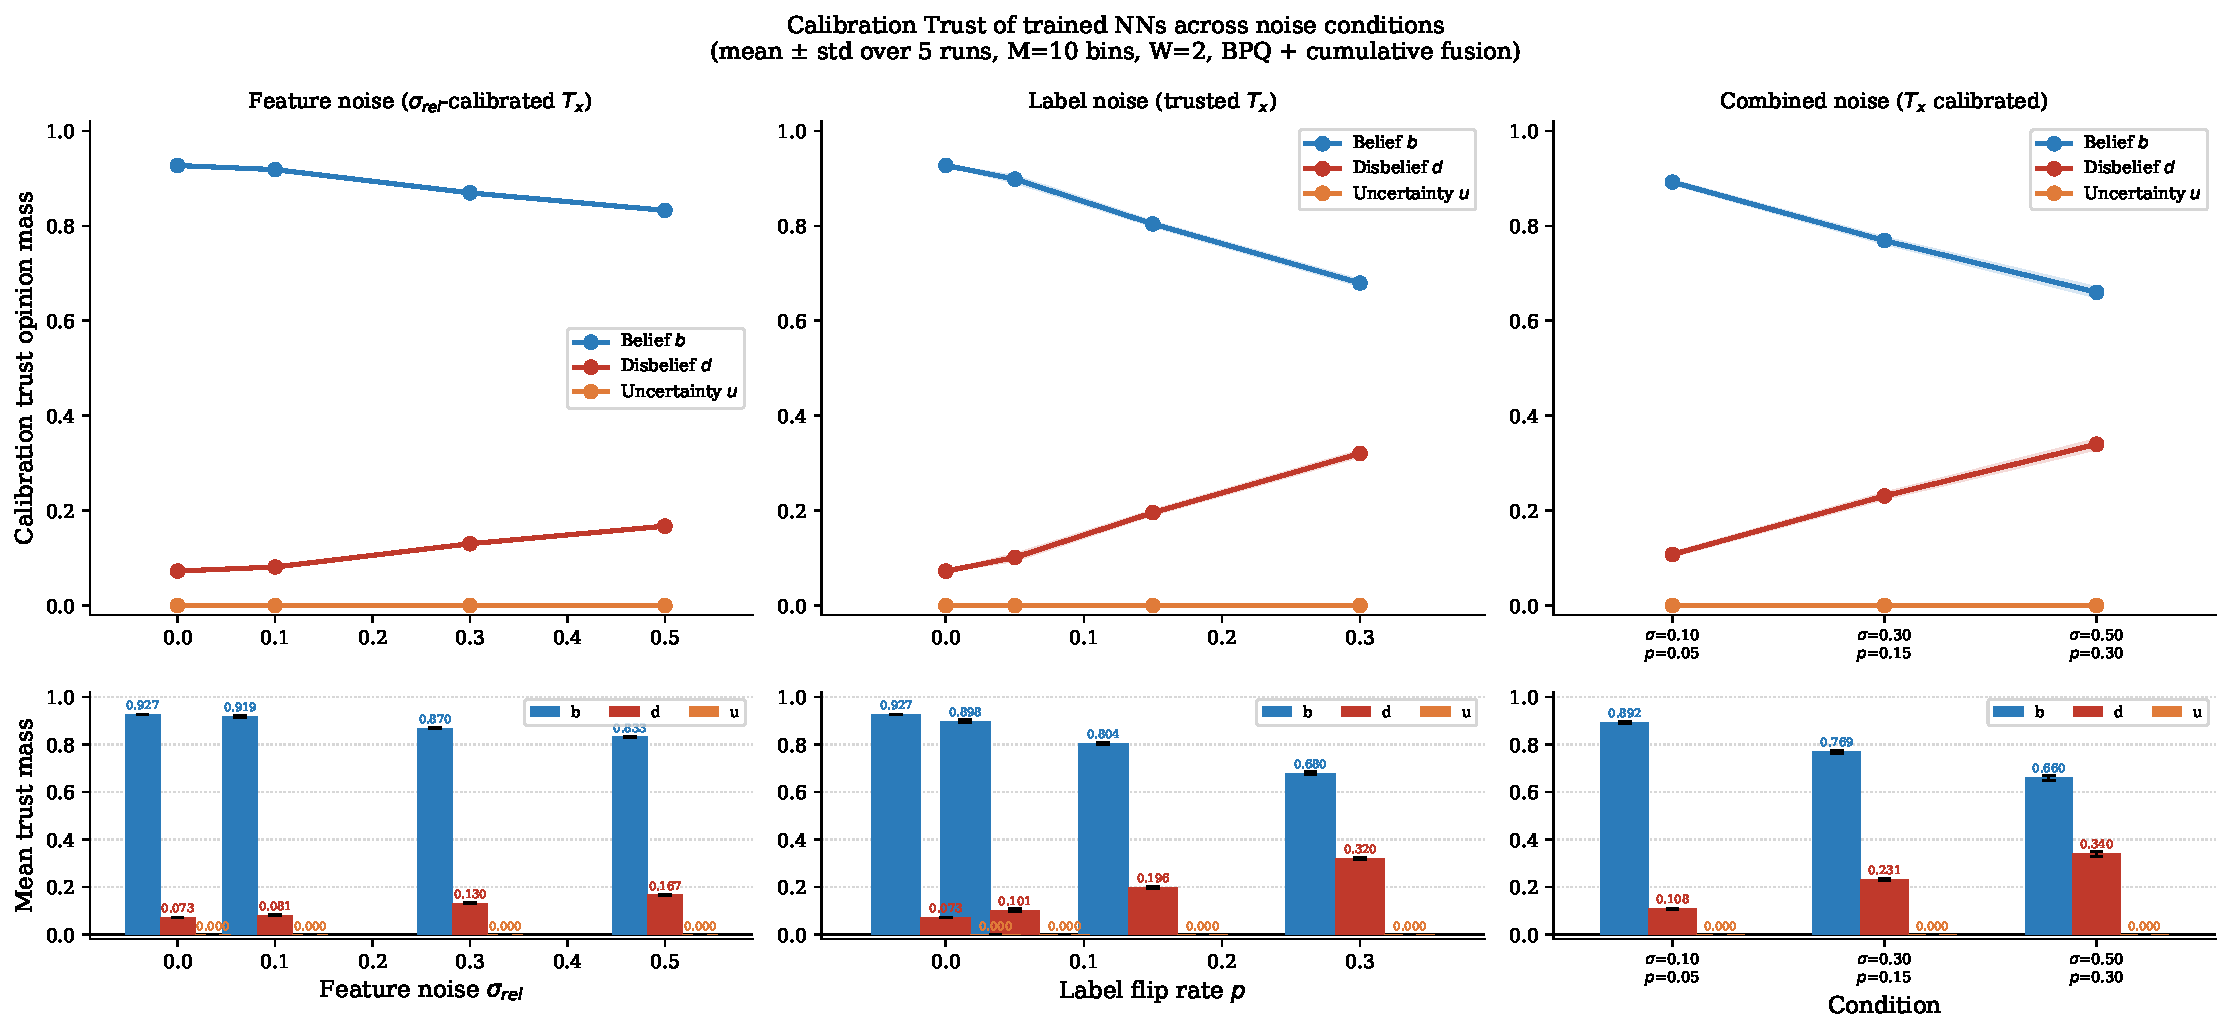
\includegraphics[width=\textwidth]{img/usecase/calibration_trust.pdf}
\begin{subfigure}{0.49\textwidth}
    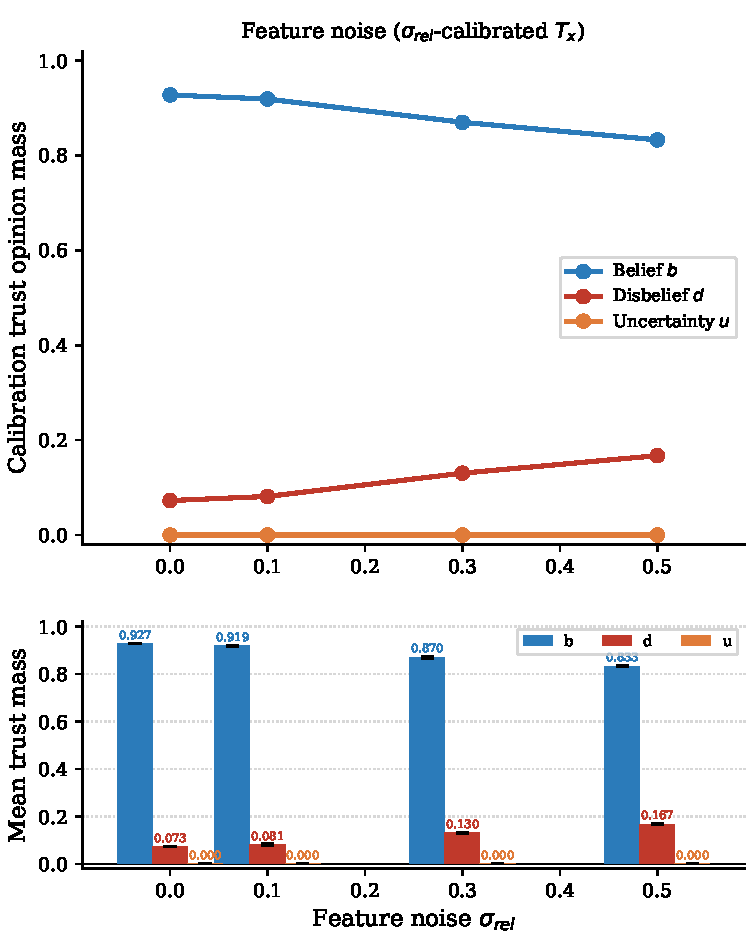
\includegraphics[width=\textwidth]{img/usecase/calibration_trust_cropped_1.pdf}
\end{subfigure}
\begin{subfigure}{0.49\textwidth}
    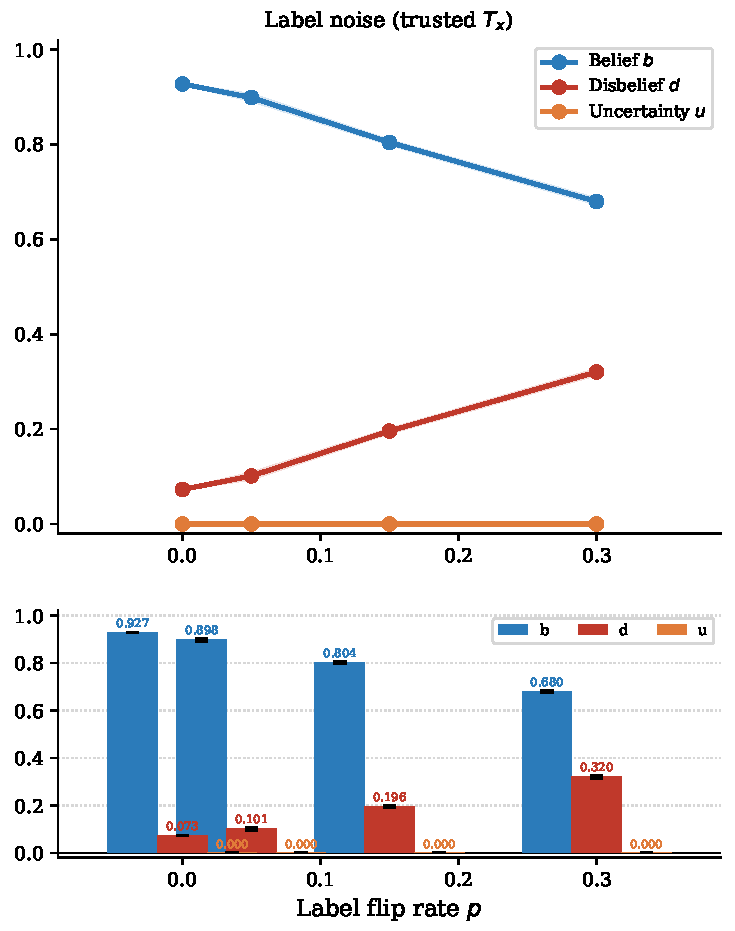
\includegraphics[width=\textwidth]{img/usecase/calibration_trust_cropped_2.pdf}
\end{subfigure}
\begin{subfigure}{0.49\textwidth}
    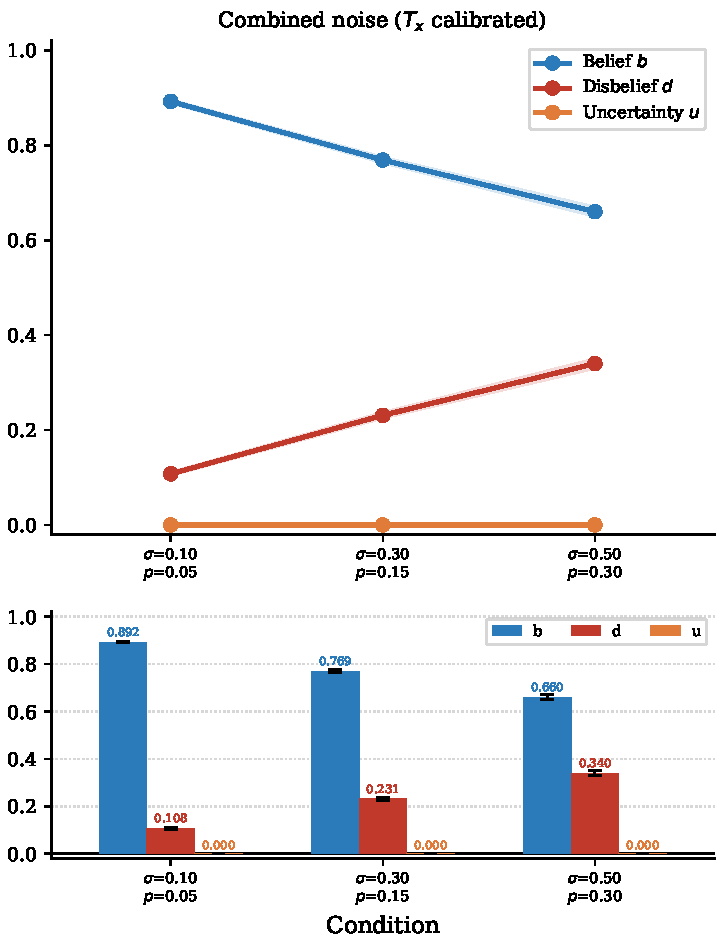
\includegraphics[width=\textwidth]{img/usecase/calibration_trust_cropped_3.pdf}
\end{subfigure}
\caption{Calibration trust of trained NNs across noise conditions, computed via BPQ with cumulative fusion ($M = 10$ bins, $W = 2$). Top: opinion masses as a function of noise magnitude. Bottom: numerical values per condition. Left: feature noise. Center: label noise. Right: combined noise. Mean $\pm$ standard deviation over 5 independent runs.}
\label{fig:calibration_trust}
\end{figure}

\begin{table}[ht]
\centering
\caption{calibration-trust opinions for trained NNs across noise conditions. Opinions averaged over 5 independent runs. High belief $b$ indicates a well-calibrated, trustworthy model; high uncertainty $u$ indicates insufficient evidence.}
\label{tab:calibration-trust}
\begin{tabular}{lcccc}
\toprule
Condition & Belief $b$ (mean$\pm$std) & Disbelief $d$ (mean$\pm$std) & Uncertainty $u$ (mean$\pm$std)\\
\hline
Feature noise \\
0.00 & 0.93$\pm$0.00 & 0.07$\pm$0.00 & 0.01$\pm$0.00 \\
0.10 & 0.93$\pm$0.01 & 0.08$\pm$0.01 & 0.01$\pm$0.01 \\
0.30 & 0.87$\pm$0.01 & 0.13$\pm$0.01 & 0.01$\pm$0.00 \\
0.50 & 0.83$\pm$0.01 & 0.17$\pm$0.01 & 0.01$\pm$0.00 \\
\hline 
Label noise  \\
0.00 & 0.93$\pm$0.00 & 0.07$\pm$0.00 & 0.01$\pm$0.00 \\
0.05 & 0.90$\pm$0.01 & 0.10$\pm$0.01 & 0.01$\pm$0.00 \\
0.15 & 0.80$\pm$0.01 & 0.20$\pm$0.01 & 0.01$\pm$0.00 \\
0.30 & 0.68$\pm$0.02 & 0.32$\pm$0.01 & 0.01$\pm$0.00\\
\hline
Combined noise \\
(0.10,0.05) & 0.89$\pm$0.01 & 0.11$\pm$0.01 & 0.01$\pm$0.00 \\
(0.30,0.15) & 0.77$\pm$0.01 & 0.23$\pm$0.01 & 0.01$\pm$0.00  \\
(0.50,0.30) & 0.66$\pm$0.01 & 0.34$\pm$0.01 & 0.01$\pm$0.00 \\
\bottomrule
\end{tabular}
\end{table}

\paragraph{Feature noise has limited impact on calibration.}
As $\sigma_{\text{rel}}$ increases from $0$ to $0.5$, belief decreases only modestly from $0.927$ to $0.833$, while disbelief rises from $0.073$ to $0.167$. The model remains well-calibrated despite degraded inputs, indicating that its confidence values continue to track empirical accuracy even when the underlying data is noisier. This is consistent with the graceful accuracy degradation seen in \Cref{sec:baseline_nn}. \todo{Add also that noise adding is a differential privacy\cite{} way to avoid overconfidence. so noise is not so bad}

\paragraph{Label noise causes substantial miscalibration.}
Label flipping has a much stronger effect: at $p = 0.30$, belief drops to $0.680$ and disbelief rises to $0.320$. When training labels are systematically wrong, the model learns to be confident in incorrect predictions, breaking the alignment between predicted probabilities and true accuracy. Calibration trust correctly identifies this as the more severe form of corruption.

\paragraph{Combined noise compounds the effect.}
Under combined corruption, calibration trust degrades faster than under either source alone. At $(\sigma, p) = (0.50, 0.30)$, belief falls to $0.660$, the lowest across all conditions. The dominant driver is label noise, with feature noise contributing additively but secondarily.

\paragraph{Uncertainty remains negligible.}
Across all conditions, uncertainty $u$ stays near $10^{-4}$. With a large test set (over 18{,}000 samples distributed across $M = 10$ bins and 3 classes), the evidence weight $W = 2$ becomes negligible relative to the cumulative evidence, driving $u \to 0$. The opinion collapses toward a Beta distribution with well-determined belief and disbelief, leaving little residual uncertainty.


\subsection{Comparison: Per-Prediction Trust vs.\ Calibration Trust}
\label{sec:patas_vs_calibration}

PaTAS opinions and calibration-trust opinions answer different questions about the same trained network. \Cref{tab:trust_comparison} summarizes the distinction.

\begin{table}[h]
\centering
\caption{Per-prediction trust (PaTAS) versus global calibration trust.}
\label{tab:trust_comparison}
\begin{tabular}{lll}
\toprule
Aspect & PaTAS (per-prediction) & Calibration trust (global) \\
\midrule
Granularity & One opinion per sample & One opinion per model \\
Computation & Forward through \ac{TNN} & Post-hoc on predictions \\
Dominant component & Uncertainty (feature noise) & Dis/belief (miscalibration) \\
Use case & Selective prediction & Model auditing \\
% Signal at high noise & Degrades to vacuous & Degrades to high disbelief \\
\bottomrule
\end{tabular}
\end{table}

The two methods complement each other. PaTAS opinions express \emph{uncertainty about a specific prediction} given the input quality: a high-uncertainty PaTAS opinion suggests the input itself is unreliable. Calibration-trust opinions express \emph{belief/disbelief in the model's confidence calibration} given its observed accuracy: a high-disbelief or low belief calibration opinion suggests the model is miscalibrated and its confidence values cannot be trusted. Used together, the two trust assessments provide a comprehensive picture: PaTAS identifies which predictions to trust at inference time; calibration trust assesses whether to trust the model as a whole in terms of score predicted.


\section{Discussion}
\label{sec:discussion}


\subsection{What PaTAS Adds Beyond Softmax Confidence}
\label{sec:discussion_softmax}

Softmax probabilities collapse confidence into a single number, while PaTAS produces a three-component opinion $(b, d, u)$. This distinction is meaningful for several reasons:

\begin{itemize}
    \item \textbf{Uncertainty separation.} PaTAS distinguishes between low confidence due to insufficient evidence (high $u$, low $d$) and low confidence due to conflicting evidence (low $u$, high $d$). Softmax conflates these into a single low-probability output.
    \item \textbf{Traceable origins.} Because PaTAS opinions are constructed by propagating input opinions through the network, uncertainty in a prediction can be traced back to specific noisy inputs or unreliable parameters.
    \item \textbf{Operational interpretation.} The components $(b, d, u)$ map to distinct decisions: high $u$ suggests collecting more data; high $d$ suggests auditing the labeling process.
\end{itemize}


\subsection{Computational Cost}
\label{sec:computational_cost}

We measured the latency overhead of running PaTAS alongside the standard neural network, both at inference and during training. The results are summarized in \Cref{fig:patas_latency}, with detailed numbers in \Cref{tab:latency-inference,tab:latency-training}.

\begin{figure}[h]
\centering
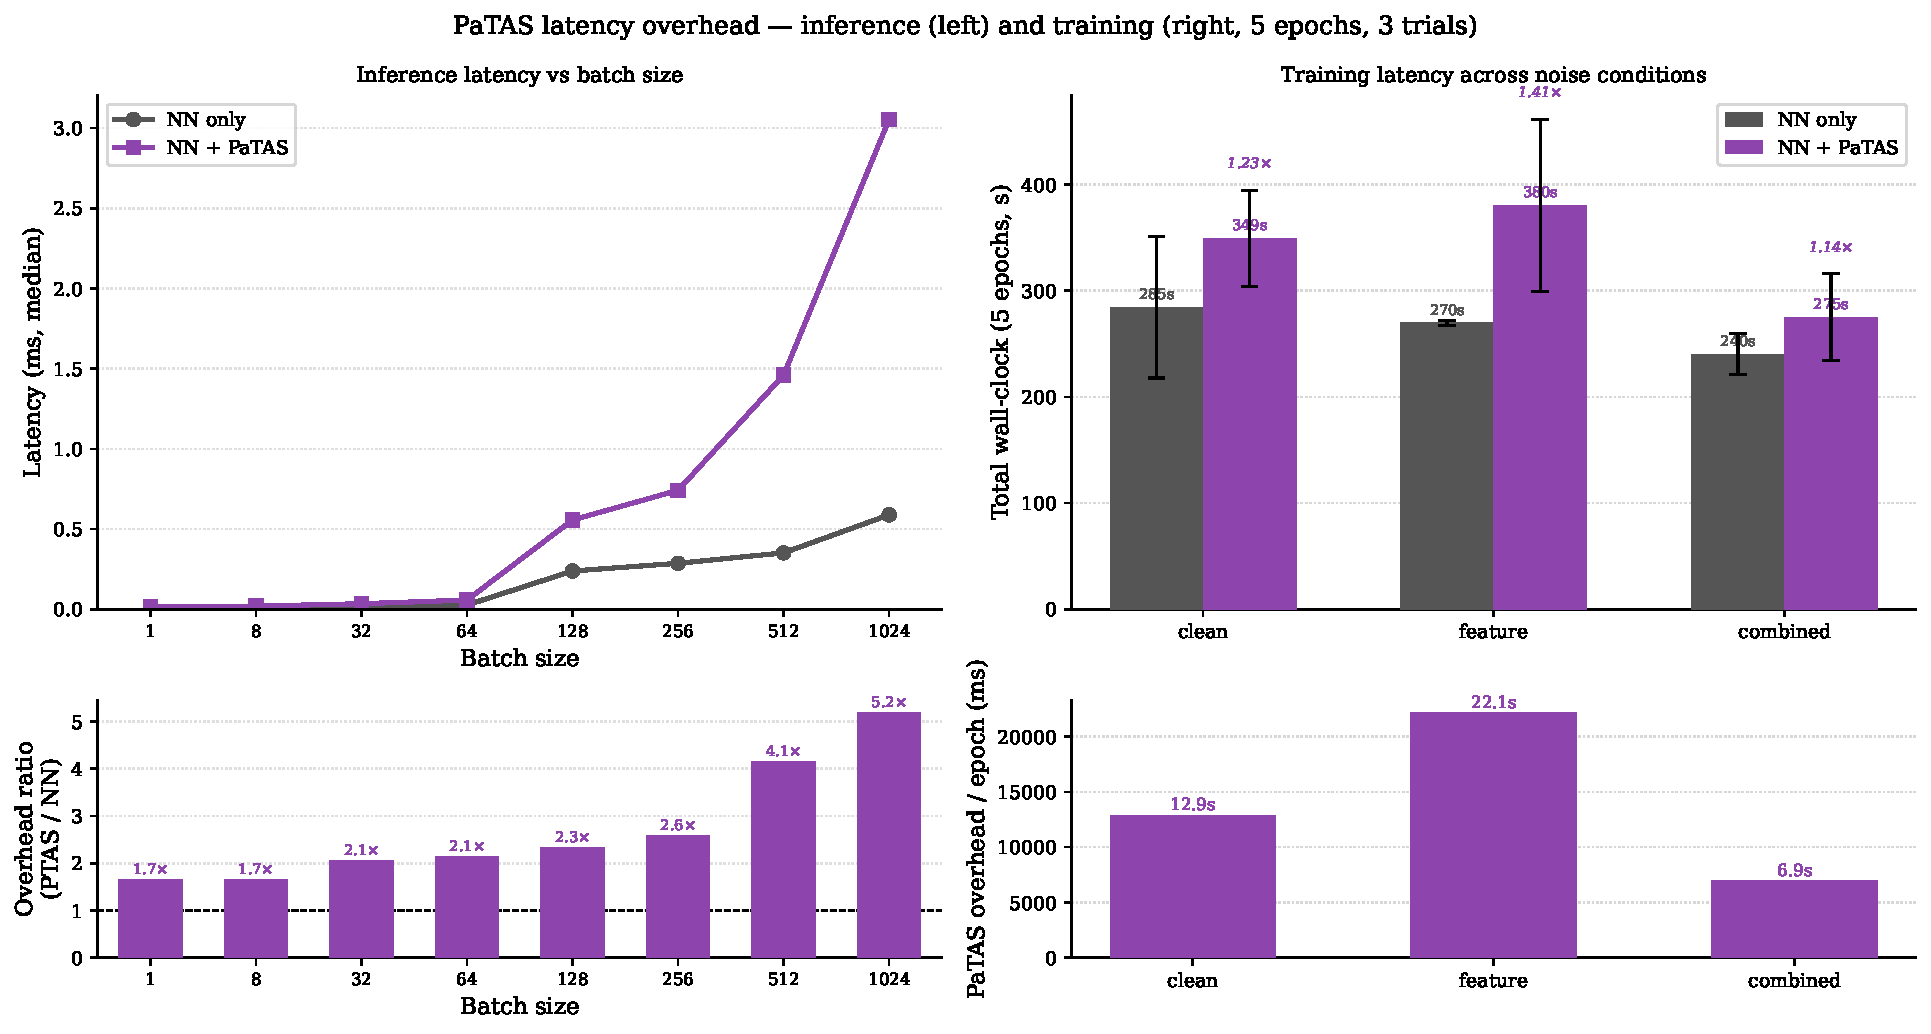
\includegraphics[width=\textwidth]{img/usecase/latency_plot.pdf}
\caption{PaTAS latency overhead. Left column: inference latency as a function of batch size; the upper plot shows absolute median latency (200 repetitions), the lower plot shows the PaTAS-to-NN overhead ratio. Right column: training wall-clock across noise conditions (mean $\pm$ std over 3 trials, 5 epochs each); the upper plot shows total time, the lower plot shows the per-epoch PaTAS overhead in milliseconds.}
\label{fig:patas_latency}
\end{figure}



\begin{table}[ht]
\centering
\caption{Training latency (mean $\pm$ std over 3 trials, 5 epochs) for plain NN vs PaTAS-augmented NN training. Overhead / epoch = per-epoch wall-clock difference.}
\label{tab:latency-training}
\begin{tabular}{lcccccc}
\toprule
Condition & NN tot(s) & PaTAS tot(s) & NN/ep(s) & PaTAS/ep(s) & Overhead/ep(ms) & Ratio($\times$) \\
\midrule
clean & 284.6$\pm$66.8 & 348.9$\pm$45.3 & 56.91 & 69.79 & 12874 & 1.23 \\
feature & 269.7$\pm$2.4 & 380.4$\pm$80.8 & 53.93 & 76.08 & 22144 & 1.41 \\
combined & 240.2$\pm$19.5 & 275.0$\pm$40.9 & 48.05 & 54.99 & 6944 & 1.14 \\
\bottomrule
\end{tabular}
\end{table}


\begin{table}[ht]
\centering
\caption{Inference latency (median over 200 repetitions) for plain NN forward pass vs PaTAS \texttt{apply\_feedforward}. Overhead ratio = PaTAS / NN.}
\label{tab:latency-inference}
\begin{tabular}{lccc}
\toprule
Batch size & NN latency (ms) & PaTAS latency (ms) & Overhead ratio ($\times$) \\
\midrule
1 & 0.009 & 0.015 & 1.66 \\
8 & 0.012 & 0.02 & 1.794 \\
32 & 0.017 & 0.035 & 2.044 \\
64 & 0.027 & 0.058 & 2.156 \\
128 & 0.239 & 0.557 & 2.330 \\
256 & 0.287 & 0.742 & 2.585 \\
512 & 0.352 & 1.460 & 4.15 \\
1024 & 0.589 & 3.054 & 5.189 \\
\bottomrule
\end{tabular}
\end{table}





\paragraph{Inference latency.}
At small batch sizes ($\leq 64$), PaTAS adds an absolute overhead of well under 0.1\,ms, with the relative overhead ratio between 1.7$\times$ and 2.2$\times$. At these sizes, both the NN forward pass and the trust feedforward through the Trust Nodes Network are dominated by per-call constants rather than by the size of the batch. As batch size grows, the overhead ratio increases more steeply: 2.6$\times$ at batch 256, 4.1$\times$ at batch 512, and 5.2$\times$ at batch 1024. In absolute terms, PaTAS adds roughly 2.5\,ms per inference at batch size 1024 (3.05\,ms total versus 0.59\,ms for the NN alone). This scaling reflects the fact that the trust discounting operator applied at each Trust Node performs more work per sample than a standard matrix multiplication: each sample carries a $(b, d, u)$ triple that must be discounted by the weight opinion at every neuron, accumulated, and combined across inputs.


\paragraph{Training overhead.}
Training overhead is more moderate than the inference overhead suggests, because the trust update step runs in parallel with the NN's backward pass over the TCP socket rather than blocking it. Over 5 epochs and 3 trials, total training time increased by 1.14$\times$ to 1.41$\times$ depending on the noise condition: 1.23$\times$ on clean data (285\,s $\to$ 349\,s), 1.41$\times$ under feature noise (270\,s $\to$ 380\,s), and 1.14$\times$ under combined noise (240\,s $\to$ 275\,s). The per-epoch overhead ranges from 6.9\,s to 22.1\,s. The variability across conditions (especially the high standard deviation on the clean and feature settings) reflects the TCP-based client-server architecture: trust message exchange is sensitive to scheduling, socket buffering, and process contention, all of which contribute additional jitter.


\paragraph{Implications for deployment.}
Three implications follow:

\begin{itemize}
    \item \textbf{Inference cost is acceptable for moderate batch sizes.} At batch sizes typical of streaming inference ($\leq 64$), the absolute overhead is sub-millisecond, well within typical service-level budgets. PaTAS is therefore practical for per-sample or small-batch deployment, which is the regime in which its per-prediction trust signal is most useful.
    \item \textbf{Large-batch inference incurs proportionally higher cost.} The 5.2$\times$ overhead at batch 1024 suggests that batched offline scoring with PaTAS should be reserved for cases where the trust signal is genuinely needed (for instance, periodic audits or selective prediction over a large dataset).
    \item \textbf{Training cost is dominated by the NN itself.} The 1.14--1.41$\times$ training overhead is modest given that PaTAS maintains an entire parallel Trust Nodes Network and exchanges opinions every batch. For most settings, a one-time training cost of this magnitude is acceptable, particularly given that PaTAS-augmented training produces an interpretable trust signal at no additional inference cost beyond the values reported above.
\end{itemize}

These measurements were taken on a single machine running both processes over a local TCP socket; production deployments could reduce overhead further by replacing the socket transport with shared-memory or in-process integration, at the cost of tighter coupling between the NN and PaTAS code.

\subsection{Limitations}
\label{sec:limitations}

\begin{itemize}
    \item \textbf{Network depth}: We use a shallow 2-layer MLP. Trust propagation in deeper architectures may exhibit different dynamics, particularly because trust discounting compounds across layers.
   
    \item \textbf{Network depth.} We use a shallow 2-layer MLP. Trust propagation in deeper architectures may exhibit different dynamics, particularly because trust discounting compounds across layers.
    \item \textbf{Calibration assumptions.} The trust calibration functions ($\text{feature\_noise\_to\_trust}$ and $\text{label\_noise\_to\_trust}$) are designed for the specific noise model used in our experiments. Real-world noise may not follow these distributions, and calibration should be adapted to the application domain.
    \item \textbf{Single dataset.} Our evaluation focuses on a single domain (5G network energy). Generalization to other modalities (images, text) and tasks (regression, sequence prediction) remains future work.
\end{itemize}


\subsection{Connection to the Broader Thesis}
\label{sec:discussion_thesis}

This use case demonstrates the practical applicability of the PaTAS framework introduced in earlier chapters:

\begin{itemize}
    \item The trust quantification methodology of \cref{chap:dataset-trust} is operationalized through the calibration functions for feature and label noise.
    \item The Trust Propagation Module of the Parallel Trust Assessment System architecture (\cref{chap:patas}) is realized end-to-end through the TCP-socket-based client-server interaction.
    \item The calibration-trust framework of \cref{chap:bb} provides a complementary global trust assessment that confirms the per-prediction findings.
\end{itemize}

Together, these elements show that subjective logic can be deployed in production-style machine learning pipelines as a complement to standard probabilistic reasoning, providing interpretable, decomposable trust assessments that support downstream decision-making.


\section{Conclusion}
\label{sec:conclusion}

This chapter applied the Parallel Trust Assessment System to a real-world use case in 5G network energy classification. We addressed four research questions.


\subsubsection*{Question 1: Trust Opinion Assignment}

\emph{How should trust opinions be assigned to real-world data?}

We introduced two calibration functions that map noise characteristics to subjective opinions: $\text{feature\_noise\_to\_trust}(\sigma_{\text{rel}})$ for measurement noise (uncertainty-dominant) and $\text{label\_noise\_to\_trust}(p)$ for label-flipping errors (disbelief-dominant). These functions reflect the semantic distinction between random measurement variability and systematic labeling errors.


\subsubsection*{Question 2: Trust Propagation Dynamics}

\emph{How do trust opinions propagate through the network during training?}

Trust opinions on inputs and labels propagate through the network via the discounting and deduction operators of Subjective Logic. The forward-propagated opinion in the NN's predicted class provides a confidence signal that can be compared to softmax confidence. Crucially, trust propagation does not affect the neural network's learning trajectory: PaTAS operates as a parallel reasoning system, leaving the NN's gradients and predictions intact.


\subsubsection*{Question 3: Robustness as a Confidence Signal}

\emph{Does the trust signal produced by PaTAS reliably indicate prediction correctness under data corruption?}

Yes. PaTAS belief discriminates between correct and incorrect NN predictions, with a discriminative gap of $\Delta b = +0.28$ at low noise levels. Used as a selective prediction filter, PaTAS achieves 89.4\% accuracy on retained samples versus 84.3\% overall, substantially outperforming softmax thresholding (85.2\% on retained). The advantage holds across feature noise, label noise, and combined corruption, degrading gracefully as noise increases beyond the network's representational capacity.


\subsubsection*{Question 4: Per-Prediction Trust versus Global Calibration Trust}

\emph{How does PaTAS-based per-prediction trust relate to a global calibration-trust assessment of the same model?}

The two assessments answer complementary questions and produce consistent signals. PaTAS opinions vary per sample and are dominated by uncertainty under feature noise, allowing fine-grained selective prediction. Calibration trust produces a single per-model opinion dominated by disbelief, with strong sensitivity to label noise (belief drops from 0.93 to 0.68 as $p$ rises to 0.30) and mild sensitivity to feature noise. The fact that both methods, despite operating at different granularities and through different computational paths, produce coherent and interpretable trust signals supports the broader claim that subjective logic offers a unified framework for trust quantification in neural network systems.


\subsection*{Contributions of This Chapter}

This use case validates the framework on three dimensions:
\begin{enumerate}
    \item \textbf{Methodological:} It demonstrates how trust quantification, propagation, and aggregation operate as a coherent pipeline on real-world data.
    \item \textbf{Empirical:} It provides quantitative evidence that PaTAS opinions are discriminative and useful as a confidence signal, and that global calibration trust is sensitive to the underlying data quality.
    \item \textbf{Practical:} It shows that PaTAS can be deployed alongside an existing neural network without modifying training, offering an interpretable trust assessment layer.
\end{enumerate}

Together with the theoretical foundations established in earlier chapters, this evaluation completes the picture of trust assessment for neural network systems: from definition and quantification, through propagation and aggregation, to empirical validation in a production-relevant setting.
\chapter{Conclusion \& Future Work}
\label{chap:conclusion}
\todo[inline]{Estimated Nb Pages: 6}
\section{Summary: Synthesis of contributions}
% \section{Conceptual unification}
\section{Perspectives: outlook, future work and limitations}
% \section{Research Agenda}
\todo[inline]{How this can help for explainability, privacy, robustness and AI Trustworthiness in General}
\todo[inline]{Make clear for generative AI as in the intro}
%----------------------------------------------------------------------------------------
%	THESIS CONTENT - APPENDICES
%----------------------------------------------------------------------------------------
% \addtocontents{toc}{\protect\setcounter{tocdepth}{-1}}
\setcounter{chapter}{1}
\chapter{Background and Related Work}

\chapter{General Trust Assessment Methodology }
This chapter introduces the \emph{General Trust Assessment Methodology} that forms the conceptual backbone of this dissertation. 
The methodology builds upon earlier work on trust evaluation developed in the context of connected and autonomous systems, including the Evidence-based \ac{TAF} developed within the Horizon Europe CONNECT project~\cite{connect_d31_taf}, the 5GAA white paper on trust evaluation~\cite{5gaa_trust4cav_2025}, the trust assessment framework presented at the International Conference on Information and Communications Security (ICICS)~\cite{fotos2025actions}, and subsequent work on trustworthy data assessment presented at the Bias Workshop at ECML~\cite{ecmldatatrust}. 
In this chapter, these contributions are unified and generalized into a systematic methodology for structuring trust assessment problems and deriving trust evaluations so that it can be instantiated across different \ac{AI} contexts.



\chapter{Optimization of \acs{DSPG} Synthesis and \aclu{TNA-SL}}
This chapter presents an optimized framework for \acf{TNA-SL} which is often used to generate expression in phase 1 of the Trust Assessment methodology. The chapter introduces foundational, algorithmic, and operator level improvements that address several limitations of the classical \ac{TNA-SL} methodology. In particular, we propose a refined structural representation of trust networks based on \acf{PNPS}, derive optimized \ac{DSPG} synthesis criteria that preserve more information, develop an improved \ac{DSPG} analysis algorithm that reduces computational overhead, and introduce a new referral-edge path discounting operator ensuring consistent trust propagation over referral chains. The \acf{PNPS} structural concept was initially introduced through collaboration with colleagues at Huawei and research partners in Luxembourg. Building on this definition, all theoretical developments presented in this chapter, including the formalization, analysis, and proofs of the proposed properties and algorithms, were carried out in this work.

The results presented in this chapter are based on two peer-reviewed publications. The structural and algorithmic optimization of \ac{DSPG} synthesis and analysis were published in \cite{10.1007/978-3-032-08887-1_4} and presented at the RuleML+RR 2025 conference. The referral-edge trust discounting operator and its theoretical properties were presented in \cite{10706345} at the FUSION 2024 conference. This chapter unifies these contributions into a coherent framework for efficient and information-preserving trust inference.

\chapter{\acf{PaTAS}}
The previous chapters established the conceptual and methodological foundations for trust assessment in general and particularly in \ac{AI} systems. In particular, \cref{chap:Trust_method} introduced a general evidence-based methodology for trust evaluation, while \cref{chap:tnasl} improved the graph-based reasoning mechanisms required to compute trust expressions. Building on these foundations, this chapter introduces the \emph{\acf{PaTAS}}, a system architecture designed to operationalize the proposed methodology in \ac{ML} pipelines. \ac{PaTAS} provides a scalable and modular framework for performing trust assessment throughout both training and inference, starting from the training dataset. The system enables the evaluation of \ac{NN} outputs in parallel with their inference by allowing different trust sources and reasoning components to be processed independently, without impacting the standard \ac{NN} inference process. This design allows efficient evaluation of trust in complex \ac{NN} systems where multiple evidence streams must be combined. The concepts presented in this chapter build upon previous publication. In particular, the architecture and core reasoning principles are derived from the work presented in~\cite{patas}, currently under review at the \emph{Elsevier Knowledge Based Systems}.

\chapter{Definition and Assessment of AI Training Datasets Trustworthiness}
\label{chap:data}
The previous chapter presented the overall architecture of \ac{PaTAS}, highlighting its two main components: (i) the Trust Assessment Module focusing on the assessment of the
trustworthiness of the training dataset and the input of the \ac{NN}, and (ii) the Trust Propagation Module focusing on the propagation of trust through the model, from the training data to the learned parameters and from the input to the output via these parameters. This chapter focuses on the first component, namely the trust assessment module. The underlying ideas were initially explored in paper presented at the Bias Workshop at ECML~\cite{ecmldatatrust} and further discussed in the position paper~\cite{trust-aidatatrust}. In this dissertation, these contributions are unified and extended to provide a comprehensive and formal framework for assessing the trustworthiness of training datasets and input data of a \ac{NN}.

\chapter{Trust Propagation in Neural Network}
The previous \cref{chap:ovl} presented the overall architecture of \ac{PaTAS}, highlighting its two main components: (i) the assessment of trust in the data, and (ii) the propagation of trust through the model, from the training data to the learned parameters and from the input to the output via these parameters. While the trustworthiness of the data was addressed in the preceding chapter, this chapter focuses on the second component, namely the propagation of trust within \aclu{NN}. In particular, it details how trust, initially derived from the dataset, is integrated into the model parameters during training and subsequently propagated from the input to the output during inference. This chapter formalizes the mechanisms that enable consistent and interpretable trust propagation across the different stages of the learning process, providing the operational core of the \ac{PaTAS} framework.

\chapter{Use Case: Applying the Trust Assessment Methodology to ...}
\noindent
The previous chapters introduced the theoretical foundations and system architecture required to perform trust assessment in \ac{NN} systems. In particular, \cref{chap:Trust_method} presented a general methodology for evidence-based trust evaluation, \cref{chap:tnasl} developed the graph-based reasoning framework for trust expression evaluation, and \cref{chap:ovl,chap:data,chap:patas} introduced the \ac{PaTAS} architecture for scalable trust assessment through the whole \ac{NN} system pipeline. This chapter demonstrates how these can be applied in practice through a concrete use case. The objective is not to introduce new theoretical contributions, but rather to illustrate how the proposed methodology can be applied to assess trustworthiness properties within a realistic \ac{ML} scenario. By instantiating the full trust assessment pipeline, from trust proposition definition to evidence collection, opinion quantification, and reasoning, we show how the framework can support practical decision-making regarding the
trustworthiness of \ac{ML} systems. The use case highlights how different trust sources can be integrated, how evidence is translated into subjective opinions, and how the resulting trust expressions can be evaluated within the proposed framework. This demonstration provides an end-to-end view of the trust assessment process and illustrates the practical relevance of the work developed throughout this dissertation.

\chapter{Calibration-Based Trust Assessment of Neural Networks}
\noindent
The previous chapters introduced and evaluated a framework for assessing the trustworthiness of \ac{NN} systems through its pipeline based on its internal behaviour. However, in many practical settings \ac{ML} models are deployed as black boxes, making it difficult to assess trust based on internal components or training processes. In such cases, trust must be inferred from observable properties of the model. One important property is calibration, which measures the alignment between predicted probabilities and empirical outcomes. In this chapter, we propose a method to quantify \ac{NN} calibration within the Evidence based \aclu{TAF} introduced in this dissertation. This chapter builds on work published and presented at the International Conference on Information Fusion (Fusion 2025)\cite{11124121}.



\chapter*{Publications}
% \addcontentsline{toc}{Publications}
\addchaptertocentry{Publications}
Each contribution presented in this thesis, particularly those addressing the research question, is supported by one or more peer-reviewed publications, demonstrating its validation and dissemination within the scientific community. As part of this publication-based doctoral thesis, these works have been published in international conference proceedings and journal articles, and are listed below.
\begin{refcontext}[labelprefix=P]
\printbibliography[category=ouattara,heading=none]
\end{refcontext}

Some of these contributions have also been disseminated as technical reports and white papers:
\begin{refcontext}[labelprefix=W]
\printbibliography[category=ouattaraRep,heading=none]
\end{refcontext}


The author has also co-authored and lead several other peer-reviewed papers related to the broader research topic. Although these works are not part of the core contributions of this thesis, they are listed here for completeness:

\begin{refcontext}[labelprefix=K]
\printbibliography[category=ouattaraAll,heading=none]
\end{refcontext}



\addchaptertocentry{Bibliography}
\printbibliography

\appendix % Cue to tell LaTeX that the following "chapters" are Appendices

% Include the appendices of the thesis as separate files from the Appendices folder
% Uncomment the lines as you write the Appendices

% Appendix: PaTAS-TP theorems and proofs

\chapter{\ac{PaTAS-TP} Theorems and Proofs (\cref{sec:ptastheory})}\label{app:proof}

Throughout this appendix, opinions are binomial, $\omega = (b, d, u)$ with $b + d + u = 1$ and a common base rate $a = 1/2$ unless stated otherwise, and $q = (b_q, d_q, u_q)$ denotes a fixed evidence opinion. The revision sequences studied are of the form $\omega_{n+1} = \omega_n \circleddash q$ for a fusion operator $\circleddash$; the operators are those of \cref{sec:fusion}. None of them makes the set of opinions a group (\cref{sec:ptas_convergence}), so convergence is established operator by operator.

\section{Revision with a Constant Evidence Opinion}

\begin{theorem}[Averaging and weighted revision]\label{thm:abf}
Let $\omega_{n+1} = \omega_n \,\underline{\oplus}\, q$ (averaging belief fusion, \cref{def:averaging_fuse}) with $\omega_0$ arbitrary and $0 < u_0 \le 1$.
\begin{enumerate}
    \item If $q$ is not vacuous ($u_q < 1$), then $\omega_n \to q$, and the convergence is geometric: $1/u_{n} - 1/u_q = 2^{-n}\,(1/u_0 - 1/u_q)$ and $|b_{n+1} - b_q| = \frac{u_q}{u_n + u_q}\,|b_n - b_q|$, the contraction factor tending to $1/2$.
    \item If $q$ is vacuous ($u_q = 1$), then $\omega_n \to (0, 0, 1)$: the evidence of $\omega_0$ is halved at every step, $1/u_n - 1 = 2^{-n}\,(1/u_0 - 1)$.
\end{enumerate}
The same limit $q$ is obtained under weighted belief fusion $\hat{\oplus}$ (\cref{def:weighted_fuse}) when $q$ is not vacuous, whereas a vacuous $q$ leaves $\omega_0$ unchanged under weighted fusion.
\end{theorem}
\begin{proof}
For averaging fusion with $u_n + u_q > 0$,
\[
u_{n+1} = \frac{2\, u_n u_q}{u_n + u_q}, \qquad
b_{n+1} = \frac{b_n u_q + b_q u_n}{u_n + u_q}, \qquad
d_{n+1} = \frac{d_n u_q + d_q u_n}{u_n + u_q}.
\]
Taking reciprocals in the first relation gives $1/u_{n+1} = \tfrac12\,(1/u_n + 1/u_q)$, an affine recursion in $1/u_n$ with fixed point $1/u_q$ and contraction factor $1/2$, which proves the statements on $u_n$ in both cases. For the belief, $b_{n+1} - b_q = (b_n - b_q)\, u_q/(u_n + u_q)$, and $u_q/(u_n + u_q) \to 1/2 < 1$ when $u_q < 1$, so $b_n \to b_q$ geometrically; the same computation applies to $d_n$. When $u_q = 1$, $b_{n+1} = b_n/(u_n + 1)$ with $u_n \to 1$, so $b_n \to 0$, and likewise $d_n \to 0$. Note that a strictly decreasing distance to $q$ alone would not prove convergence \emph{to} $q$; the explicit contraction factors do. For weighted fusion the uncertainty obeys $u_{n+1} = (2 - u_n - u_q)\, u_n u_q / (u_n + u_q - 2 u_n u_q)$. For $u_q < 1$ this map is increasing on $(0,1]$ and its value lies strictly between $u_n$ and $u_q$, so $u_n \to u_q$ monotonically; the belief and disbelief recursions are convex combinations of $(b_n, d_n)$ and $(b_q, d_q)$ whose weight on $(b_n, d_n)$ tends to $1/2$, hence they converge to $(b_q, d_q)$ as above. When $u_q = 1$ the vacuous opinion is the neutral element of weighted fusion, so $\omega_n = \omega_0$.
\end{proof}

\begin{theorem}[Cumulative revision]\label{thm:cbf}
Let $\omega_{n+1} = \omega_n \oplus q$ (cumulative belief fusion, \cref{def:cumulative_fuse}) with $0 < u_0 \le 1$.
\begin{enumerate}
    \item If $q$ is not vacuous, then $1/u_n = 1/u_0 + n\,(1/u_q - 1)$, so $u_n \to 0$ like $1/n$, and $\omega_n$ converges to the dogmatic opinion $(b_q, d_q, 0)/(b_q + d_q)$: the initial opinion $\omega_0$ is forgotten.
    \item If $q$ is vacuous, then $\omega_n = \omega_0$ for all $n$, the vacuous opinion being the neutral element of cumulative fusion.
\end{enumerate}
\end{theorem}
\begin{proof}
Cumulative fusion adds evidence: in terms of the evidence parameters $r = W b/u$ and $s = W d/u$ of an opinion (Beta--opinion mapping with prior weight $W$), $\omega_n \oplus q$ has evidence $(r_n + r_q,\; s_n + s_q)$. Hence $r_n = r_0 + n\, r_q$, $s_n = s_0 + n\, s_q$ and $u_n = W/(W + r_n + s_n)$. Since $1/u = 1 + (r + s)/W$ and $r_q + s_q = W\,(1 - u_q)/u_q$, this gives the stated expression for $1/u_n$, and $u_n \to 0$ unless $r_q = s_q = 0$, that is, unless $q$ is vacuous. Then $b_n = r_n/(W + r_n + s_n) \to r_q/(r_q + s_q) = b_q/(b_q + d_q)$, and likewise for $d_n$. If $q$ is vacuous the evidence is unchanged. For example, $q = (0.5, 0, 0.5)$ drives every non-dogmatic $\omega_0$ to $(1, 0, 0)$.
\end{proof}

\begin{theorem}[Belief constraint revision]\label{thm:bcf}
Let $\omega_{n+1} = \omega_n \odot q$ (belief constraint fusion, \cref{def:constraint_fuse}) with $\omega_0$ non-dogmatic and $q$ neither vacuous nor totally conflicting with $\omega_0$. Then $\omega_n$ converges to $(1, 0, 0)$ if $b_q > d_q$, to $(0, 1, 0)$ if $d_q > b_q$, and, if $b_q = d_q$, to the dogmatic opinion $(\beta, 1 - \beta, 0)$ with $\beta = (b_0 + u_0)/(b_0 + d_0 + 2 u_0)$, fixed by the plausibilities of $\omega_0$. A vacuous $q$ leaves $\omega_0$ unchanged.
\end{theorem}
\begin{proof}
Belief constraint fusion is Dempster's rule restricted to binomial opinions. Write $P_n = b_n + u_n$ and $\bar P_n = d_n + u_n$ for the plausibilities of $x$ and $\bar x$ under $\omega_n$. The unnormalised fused masses are $b_n b_q + b_n u_q + u_n b_q$, $d_n d_q + d_n u_q + u_n d_q$ and $u_n u_q$, so the plausibilities multiply: $P_{n+1} \propto P_n P_q$, $\bar P_{n+1} \propto \bar P_n \bar P_q$ and $u_{n+1} \propto u_n u_q$, all with the same normalisation constant $1/(1 - K_n)$, $K_n = b_n d_q + d_n b_q$. Therefore
\[
\frac{P_n}{\bar P_n} = \frac{P_0}{\bar P_0}\Big(\frac{b_q + u_q}{d_q + u_q}\Big)^{n}, \qquad
\frac{u_n}{P_n} = \frac{u_0}{P_0}\Big(\frac{u_q}{b_q + u_q}\Big)^{n}.
\]
If $b_q > d_q$, the first ratio diverges, so $\bar P_n = d_n + u_n \to 0$; the second ratio tends to zero because $b_q > 0$, so $u_n \to 0$, hence $d_n \to 0$ and $b_n \to 1$. The case $d_q > b_q$ is symmetric. If $b_q = d_q > 0$, the first ratio is constant, equal to $P_0/\bar P_0$, while $u_n \to 0$, so the limit is dogmatic with $b/d = P_0/\bar P_0$, which gives $\beta$. A vacuous $q$ has $K = 0$ and returns $\omega_n$ unchanged.
\end{proof}

\begin{remark}[Amplification and numerical caveat]\label{rem:bcf-numerics}
The evidence $q = (0.4, 0.35, 0.25)$ drives the sequence to $(1, 0, 0)$: a slight majority of belief over disbelief is amplified to certainty. Iterating belief constraint fusion naively in floating point is moreover unstable, because each step multiplies the rounding error of $b + d + u$ by $1/(1 - K_n)$; in a test run with this $q$ the mass sum had drifted away from $1$ after $60$ steps and collapsed below $0.01$ after $100$ steps. An implementation that iterates this operator must renormalise after every step, as the implementation of this thesis does after every operator application.
\end{remark}

\section{The Implemented Update under Trusted Data}

\begin{theorem}[Implemented update under trusted data]\label{thm:implemented}
Let \cref{alg:trustupdate} run with averaging revision, base rate $a = 1/2$, $T_{lr} = (1, 0, 0)$, and a fully trusted conditioning factor, $T_x \oslash T_{y_\text{batch}} = (1, 0, 0)$, as holds for the first layer under trusted input and label opinions. Let $q_n = (b_{q_n}, d_{q_n}, u_q)$ be the node opinion of batch $n$; its uncertainty $u_q = W / (|\mathcal{N}(i)| + W)$ does not depend on $n$. Then, for any initial opinion with $u^{(0)} > 0$,
\begin{enumerate}
    \item $u^{(n)} \to u^* = u_q / 15$ monotonically, whatever the sequence $(q_n)$;
    \item $d^{(n+1)} = \lambda_n\, d^{(n)} + (1 - \lambda_n)\, d_{q_n}$ with $\lambda_n = u_q / (u^{(n)} + u_q) \to 15/16$, so that $d^{(n)}$ is a convex combination of the past batch evidence with geometrically decaying weights, and $b^{(n)} = 1 - d^{(n)} - u^{(n)}$;
    \item if $d_{q_n} \to d_q$, then $T_\theta^{(n)} \to (1 - d_q - u_q/15,\; d_q,\; u_q/15)$.
\end{enumerate}
\end{theorem}
\begin{proof}
With base rate $1/2$, binomial multiplication (\cref{def:binomial_multiplication}) by the dogmatic opinion $(1,0,0)$ maps $(b, d, u)$ to $(b + u/3,\; d,\; 2u/3)$. The three sub-steps of one batch act on the uncertainty as follows. The revision gives $u' = 2\, u\, u_q / (u + u_q)$. The learning-rate adjustment fuses $(b, d, u')$ with $(b + u'/3,\; d,\; 2u'/3)$ by averaging fusion, which gives $u'' = 2\, u' (2u'/3) / (u' + 2u'/3) = 4u'/5$. The auxiliary adjustment multiplies by $(1,0,0)$: $u''' = 2u''/3 = 8u'/15$. Composing the three maps, $u^{(n+1)} = \varphi(u^{(n)})$ with
\[
\varphi(u) = \frac{16}{15}\cdot\frac{u\, u_q}{u + u_q},
\]
which is increasing and concave on $(0, 1]$, satisfies $\varphi(u) > u$ exactly when $u < u_q/15$ and $\varphi(u) < u$ when $u > u_q/15$. Hence $u^{(n)}$ converges monotonically to $u^* = u_q/15$ from any positive start, and $\varphi'(u^*) = 15/16 < 1$ makes the convergence geometric. Only the revision changes the disbelief: multiplication by $(1,0,0)$ leaves $d$ unchanged, and the averaging fusion of two opinions with the same disbelief returns that disbelief. Thus $d^{(n+1)} = (d^{(n)} u_q + d_{q_n} u^{(n)}) / (u^{(n)} + u_q)$, which is the stated convex combination, with $\lambda_n \to u_q/(u^* + u_q) = 15/16$. The belief follows by normalisation, and the limit in the third statement is obtained by letting $n \to \infty$ in the two recursions.
\end{proof}

\begin{remark}[Worked example and the vacuous case]\label{rem:worked}
For a neuron with $30$ incoming edges and $W = 2$, $u_q = 1/16$ and $u^* = 1/240 \approx 0.0042$. With constant evidence of $r = 27$ weak and $s = 3$ strong gradients, $q = (0.844, 0.094, 0.063)$, and a direct iteration of the released implementation converges to $(0.9021, 0.0938, 0.0042)$ within about $60$ batches, as predicted. Under cumulative revision the same iteration reaches a numerically zero uncertainty within $20$ batches (the implementation does not clip small uncertainties; in single precision the value settles at the rounding floor of the normalisation $b + d + u = 1$, about $10^{-8}$) and then freezes, since an effectively dogmatic opinion is no longer changed by a less certain one; under belief constraint revision it reaches exactly $(1, 0, 0)$ within five batches. Under a vacuous label opinion the auxiliary sub-step multiplies by $(0, 0, 1)$, which maps $(b, d, u)$ to $(b/3,\; d,\; 1 - b/3 - d)$ and expands the uncertainty instead of contracting it; the same iteration then converges to $(0.147, 0.047, 0.806)$ under averaging revision and to $(0.210, 0.183, 0.607)$ under cumulative revision. In this regime the parameter uncertainty is large and the choice of the revision operator matters. For layers beyond the first, the input opinion $T_x$ entering the auxiliary sub-step is the propagated opinion of the previous layer, which is close to but not exactly dogmatic, so the contraction is weaker and the uncertainty settles above $u_q/15$: in the breast-cancer network of Experiment~1 the mean parameter uncertainty after training is $0.005$ in the first layer and $0.06$ in the output layer.
\end{remark}

\section{Multiplicative Revision}

\begin{theorem}[Convergence of the multiplicative sequence]\label{thm:geo}
Let $\omega_{n+1} = \omega_n \odot q$ with the binomial multiplication of \cref{def:binomial_multiplication} evaluated at a fixed base rate $a \in [0,1)$ for both arguments, and write $c = a/(1+a)$ ($c = 1/3$ for $a = 1/2$). Then:
\begin{itemize}
    \item $d_{n+1} = d_n + d_q - d_n d_q$, so $d_n \to 1$ if $d_q > 0$, and $d_n = d_0$ for all $n$ if $d_q = 0$;
    \item if $d_q > 0$, then $b_n \to 0$ and $u_n \to 0$, that is, $\omega_n \to (0, 1, 0)$;
    \item if $d_q = 0$, then $b_n \to b^* = c\,(1 - d_0)\, b_q \big/ \big((1 - c)(1 - b_q) + c\, b_q\big)$, which equals $(1 - d_0)\, b_q/(2 - b_q)$ for $a = 1/2$, and $u_n \to 1 - b^* - d_0$.
\end{itemize}
\end{theorem}
\begin{proof}
With equal base rates $a$ the multiplication reads $b_{n+1} = b_n b_q + c\,(b_n u_q + u_n b_q)$, $d_{n+1} = d_n + d_q - d_n d_q$ and $u_{n+1} = 1 - b_{n+1} - d_{n+1}$. The disbelief recursion is affine with fixed point $1$ and factor $1 - d_q$; if $d_q > 0$ it converges to $1$ monotonically, and if $d_q = 0$ it is constant. If $d_q > 0$, then $0 \le b_n \le 1 - d_n \to 0$ and $0 \le u_n \le 1 - d_n \to 0$, which proves the second statement without any approximation. If $d_q = 0$, then $u_q = 1 - b_q$, $d_n = d_0$ and $u_n = 1 - b_n - d_0$, so the belief recursion becomes the affine map $b_{n+1} = \rho\, b_n + c\,(1 - d_0)\, b_q$ with $\rho = (1 - c)\, b_q + c\,(1 - b_q)$. Since $0 \le c < 1/2$, $\rho$ is a convex combination of $b_q$ and $1 - b_q$ and satisfies $\rho < 1$, so $b_n$ converges to $b^* = c\,(1 - d_0)\, b_q / (1 - \rho)$, which is the stated value; $u_n$ follows by normalisation.
\end{proof}

\section{Proof of \cref{thm:convergence}}
\begin{proof}
Statement (i) collects \cref{thm:abf,thm:cbf,thm:bcf}. Statement (ii) is \cref{thm:implemented}: under trusted data the node opinion $q_n$ enters the update only through the revision, and the theorem shows that the composed map contracts the uncertainty to $u_q/15$ independently of $(q_n)$ and turns the disbelief into a convex combination of the past $d_{q_n}$ with weights $(1 - \lambda_n)\prod_{k > n}\lambda_k$, which decay geometrically once $\lambda_n$ is close to $15/16$. If $d_{q_n}$ converges, so does this running mean, which gives the limit; if $d_{q_n}$ is stationary but fluctuating, the running mean stays within the range of the recent evidence and inherits its fluctuations, damped by the window. Statement (iii) is \cref{thm:geo}. The assumptions of stable input and label opinions enter through the auxiliary sub-step: they fix the factor $T_x \oslash T_{y_\text{batch}}$, so that the same map is applied at every batch and the fixed-point argument applies.
\end{proof}

\section{Proof of \cref{thm:infvac}}

Let \( \omega^\emptyset = (0, 0, 1, a) \) denote a vacuous binomial opinion over any variable, with arbitrary base rate \( a \in [0, 1] \). Then the following two properties hold:

\begin{enumerate}
    \item \emph{Discounting a Vacuous Opinion Yields a Vacuous Opinion.} \\
    For any trust value binomial opinion \(\omega^A_B \), the discounted opinion
    \[
    \omega^{[A;B]}_X = \omega^A_B \otimes (0,0,1,a)= (0,0,1,a)
    \]
    \textit{Proof.} Using the trust discounting operator from Subjective Logic, we set $P$ to the projected probability of \(\omega^A_B\):
    \[\omega^{[A;B]}_X =
    \begin{cases}
    b^{[A;B]}_X = P\cdot 0 = 0, \\
    d^{[A;B]}_X = P\cdot 0 = 0, \\
    u^{[A;B]}_X = 1 - b^{[A;B]}_X-d^{[A;B]}_X = 1, \\
    a^{[A;B]}_X = a.
    \end{cases}
    \]
    Hence, \( \omega^{[A;B]} = (0,0,1,a) \).

    \item \emph{PaTAS Feedforward on Vacuous Input Yields Vacuous Output.} \\
    Let \( T_x = (0,0,1,a)\) be the trust assessment of an input to PaTAS. Then for any parameter trust configuration \( T_\theta \), the output trust assessment satisfies:
    \[
    T_y = \text{IPTA}(T_x) = (0,0,1,a).
    \]
    \textit{Proof.} The PaTAS feedforward mechanism computes for each neuron:
    \[
    T_z = \bigoplus_i \left( T_{x_i} \otimes T_{\theta_i} \right).
    \]
    Since each \( T_{x_i} = (0,0,1,a) \), and using the result from part (1), we get:
    \[
    T_{x_i} \otimes T_{\theta_i} = (0,0,1,a), \quad \forall i.
    \]
    Then, by fusion of vacuous opinions (averaging fusion is idempotent, so the mean of vacuous opinions is vacuous):
    \[
    T_z = \bigoplus_i (0,0,1,a) = (0,0,1,a).
    \]
    This holds recursively through all layers of PaTAS, including the output layer, hence:
    \[
    T_y = (0,0,1,a).
    \]
\end{enumerate}

\section{Proof of \cref{thm:sym}}
\begin{proof}
We prove the theorem in two steps.

\emph{(1) Symmetry of the Discount Operator:} \\
Let $\omega_\theta = (b_\theta, d_\theta, u_\theta)$ be a binomial opinion representing the trust weight associated with a connection in the PaTAS. Let $P$ denote the projected probability of $\omega_\theta$, defined as:
\[
P = b_\theta + a u_\theta,
\]
where $a$ is the base rate (typically $a = 0.5$ for binary domains).

Let $x = (b, d, u)$ be any binomial opinion and $\bar{x} = (d, b, u)$ its symmetric counterpart. Then the trust discounting operation yields:
\[
\omega_\theta \otimes x = (P \cdot b, P \cdot d, 1 - P \cdot (b + d)),
\]
\[
\omega_\theta \otimes \bar{x} = (P \cdot d, P \cdot b, 1 - P \cdot (b + d)).
\]
Since $b + d = 1 - u$, both discounted opinions have identical uncertainty and symmetric belief/disbelief masses. Hence, $\omega_\theta \otimes x$ and $\omega_\theta \otimes \bar{x}$ are symmetric.

\emph{(2) Symmetry Preservation under Fusion:} \\
Let $\mathcal{X} = \{x_1, \dots, x_n\}$ be a set of discounted opinions resulting from symmetric inputs, and let $\bar{\mathcal{X}} = \{\bar{x}_1, \dots, \bar{x}_n\}$ be their symmetric counterparts. Consider any fusion operator $\bigoplus$ that treats belief and disbelief symmetrically (the component-wise mean used in this thesis, as well as averaging, cumulative or consensus fusion in Subjective Logic) applied to $\mathcal{X}$ and $\bar{\mathcal{X}}$.

Since each pair $(x_i, \bar{x}_i)$ is symmetric and the operator treats belief and disbelief symmetrically, we have:
\[
\bigoplus_{i=1}^n x_i = (b', d', u') \quad \Rightarrow \quad \bigoplus_{i=1}^n \bar{x}_i = (d', b', u').
\]
Thus, the output of the PaTAS feedforward inference remains symmetric when symmetric inputs are provided.

\emph{(3) Invariance under Fusion:} \\
If all input opinions assign the value zero to a specific mass (belief or disbelief), the fused result preserves that value under every operator considered here, since the fused belief (disbelief) is a weighted average of the input beliefs (disbeliefs). In particular, if all input opinions have belief mass equal to zero, the fused result also has belief mass zero. The same applies to disbelief mass.

Therefore, if the discounting step yields discounted opinions with zero belief (or zero disbelief) across all components, then the fusion stage will preserve that zero mass in the final output.

\emph{(4) Fully Trusted and Distrusted Cases:} \\
For $x = (1, 0, 0)$ (fully trusted), we have:
\[
\omega_\theta \otimes x = (P, 0, 1 - P),
\]
so the discounted opinion assigns zero disbelief. As noted above, the fusion of such discounted opinions will also assign zero disbelief.

For $\bar{x} = (0, 1, 0)$ (fully distrusted), we have:
\[
\omega_\theta \otimes \bar{x} = (0, P, 1 - P),
\]
so the discounted opinion assigns zero belief. Therefore, the belief from a fully distrusted input is always zero in the PaTAS output.
\end{proof}

\chapter{All Plots for \cref{chap:patas}}

\section*{Note on Figure Naming Convention}
\label{sec:appendixB-naming}

To keep figure captions compact throughout this appendix, each figure is
labeled with a configuration string of the form

\begin{quote}
\texttt{<dataset>\_<hidden units>\_<features op>\_<label op>\_<\(\epsilon\)>\_<patch size>}
\end{quote}

where the fields are defined as follows:

\begin{itemize}
    \item \textbf{Dataset}: the dataset used for the experiment (e.g., \texttt{cancer}, \texttt{mnist}).
    \item \textbf{Hidden units}: the number of hidden units in the network used for the experiment (e.g., \texttt{16}).
    \item \textbf{Features opinion}: the subjective-logic opinion $(b,d,u)$ assigned to the input features, given either as an explicit comma-separated triple (e.g., \texttt{0.25,0.0,0.75}) or as one of the named presets listed in Table~\ref{tab:opinion-presets}.
    \item \textbf{Label opinion}: the subjective-logic opinion $(b,d,u)$ assigned to the labels, using the same explicit-triple or named-preset notation as the features opinion.
    \item \boldmath{$\epsilon$} (optional): the sensitivity parameter used for the PaTAS plots only. Not applicable, and therefore omitted, for non-PaTAS experiments.
    \item \textbf{Patch size} (optional): the size of the poisoned patch applied to the input data, relevant only for the data-poisoning experiments. When data poisoning is not applied, this field is set to \texttt{None} (e.g., \texttt{PatchSize\_None} in the figure filenames).
\end{itemize}

For example, \texttt{cancer\_16\_0.25,0.0,0.75\_0.25,0.0,0.75} (with patch
size \texttt{None}) denotes an experiment on the \texttt{cancer} dataset
with a 16-hidden-unit network, where both features and labels were
assigned the opinion $(b,d,u) = (0.25, 0.0, 0.75)$ and no data poisoning
was applied. Similarly, \texttt{cancer\_16\_trust\_distrust} denotes the
same dataset and network size with the features opinion set to the
\emph{trust} preset and the label opinion set to the \emph{distrust}
preset (Table~\ref{tab:opinion-presets}).


For example, \texttt{cancer\_16\_0.25,0.0,0.75\_0.25,0.0,0.75} denotes an
experiment on the \texttt{cancer} dataset with a 16-hidden-unit network,
where both inputs and labels were assigned the opinion
$(b,d,u) = (0.25, 0.0, 0.75)$. Similarly,
\texttt{cancer\_16\_trust\_distrust} denotes the same dataset and network
size with the input opinion set to the \emph{trust} preset and the label
opinion set to the \emph{distrust} preset (Table~\ref{tab:opinion-presets}).

\begin{table}[h]
\centering
\caption{Named opinion presets used in figure captions throughout this appendix.}
\label{tab:opinion-presets}
\begin{tabular}{lccc}
\toprule
\textbf{Preset name} & $b$ & $d$ & $u$ \\
\midrule
trust    & 1 & 0 & 0 \\
distrust & 0 & 1 & 0 \\
vacuous  & 0 & 0 & 1 \\
\bottomrule
\end{tabular}
\end{table}

\section{NN Training Results}

\subsection{Accuracy Evolution}

\begin{figure}[htbp]
\centering
\begingroup
\captionsetup[subfloat]{justification=centering,singlelinecheck=false, font=scriptsize}
\subfloat[{cancer\_16\_0.25,0.0,0.75\_0.25,0.0,0.75}]{%
  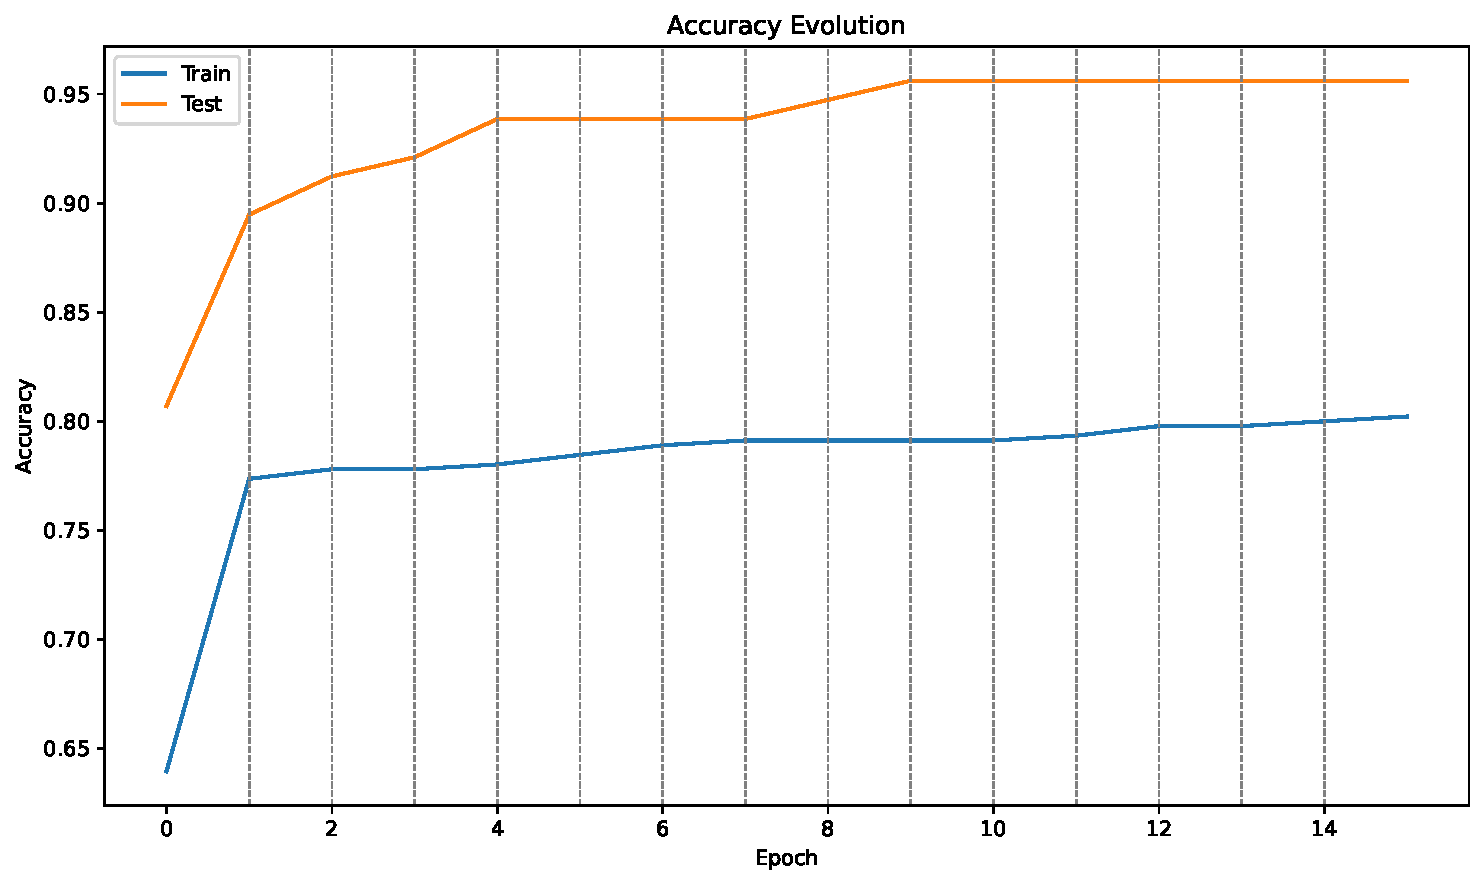
\includegraphics[width=0.3\textwidth]{latex/NN_Train_cancer_16_0.25_0.0_0.75_0.25_0.0_0.75_PathSize_None__accuracy_evolution.pdf}%
}
\subfloat[{cancer\_16\_0.25,0.25,0.5\_0.25,0.25,0.5}]{%
  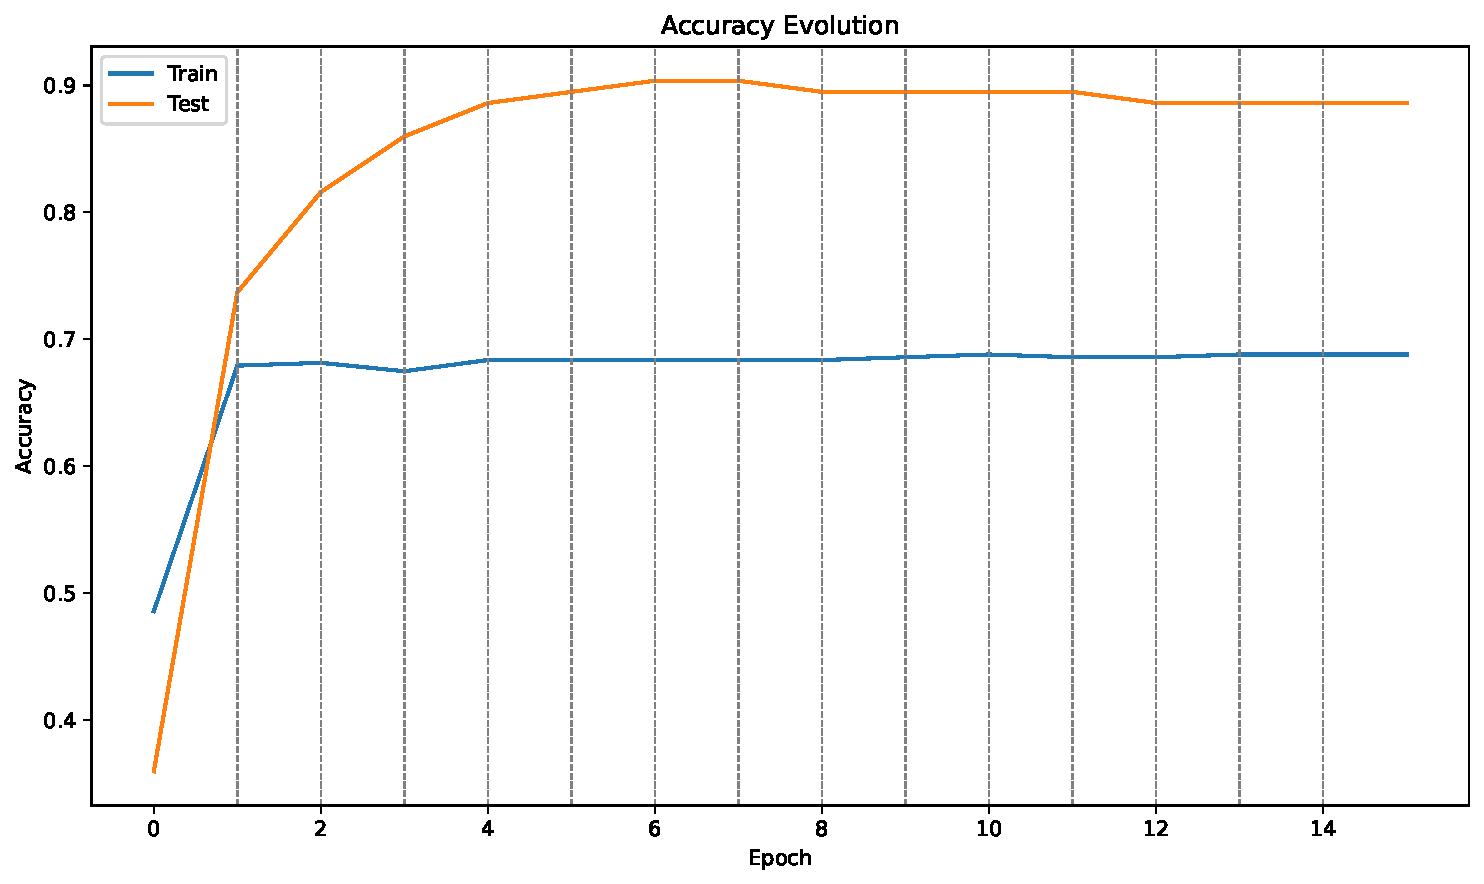
\includegraphics[width=0.3\textwidth]{latex/NN_Train_cancer_16_0.25_0.25_0.5_0.25_0.25_0.5_PathSize_None__accuracy_evolution.pdf}%
}
\subfloat[{cancer\_16\_distrust\_distrust}]{%
  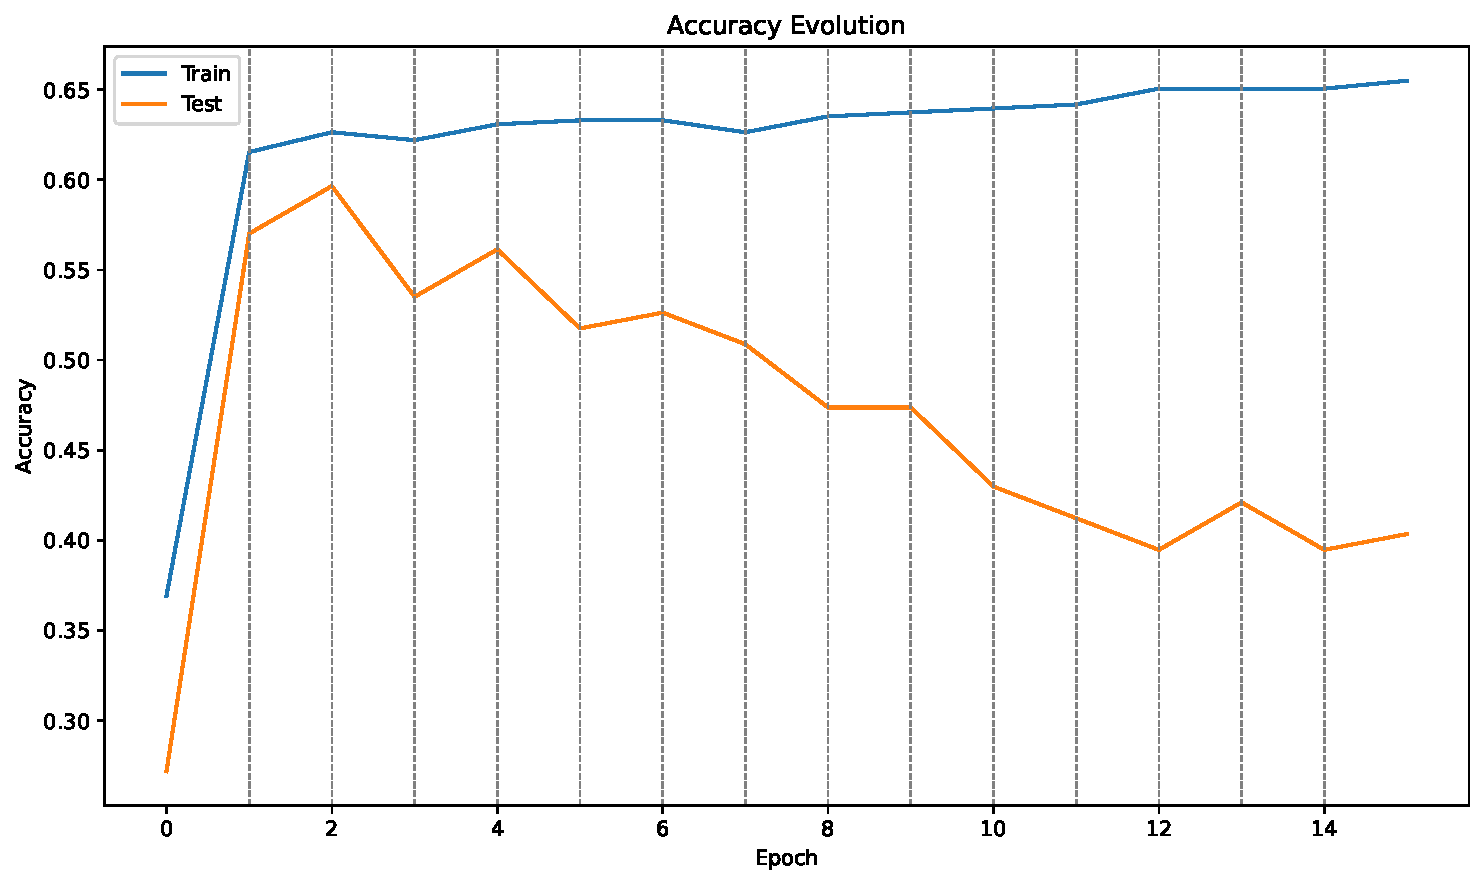
\includegraphics[width=0.3\textwidth]{latex/NN_Train_cancer_16_distrust_distrust_PathSize_None__accuracy_evolution.pdf}%
}
\\
\subfloat[{cancer\_16\_distrust\_trust}]{%
  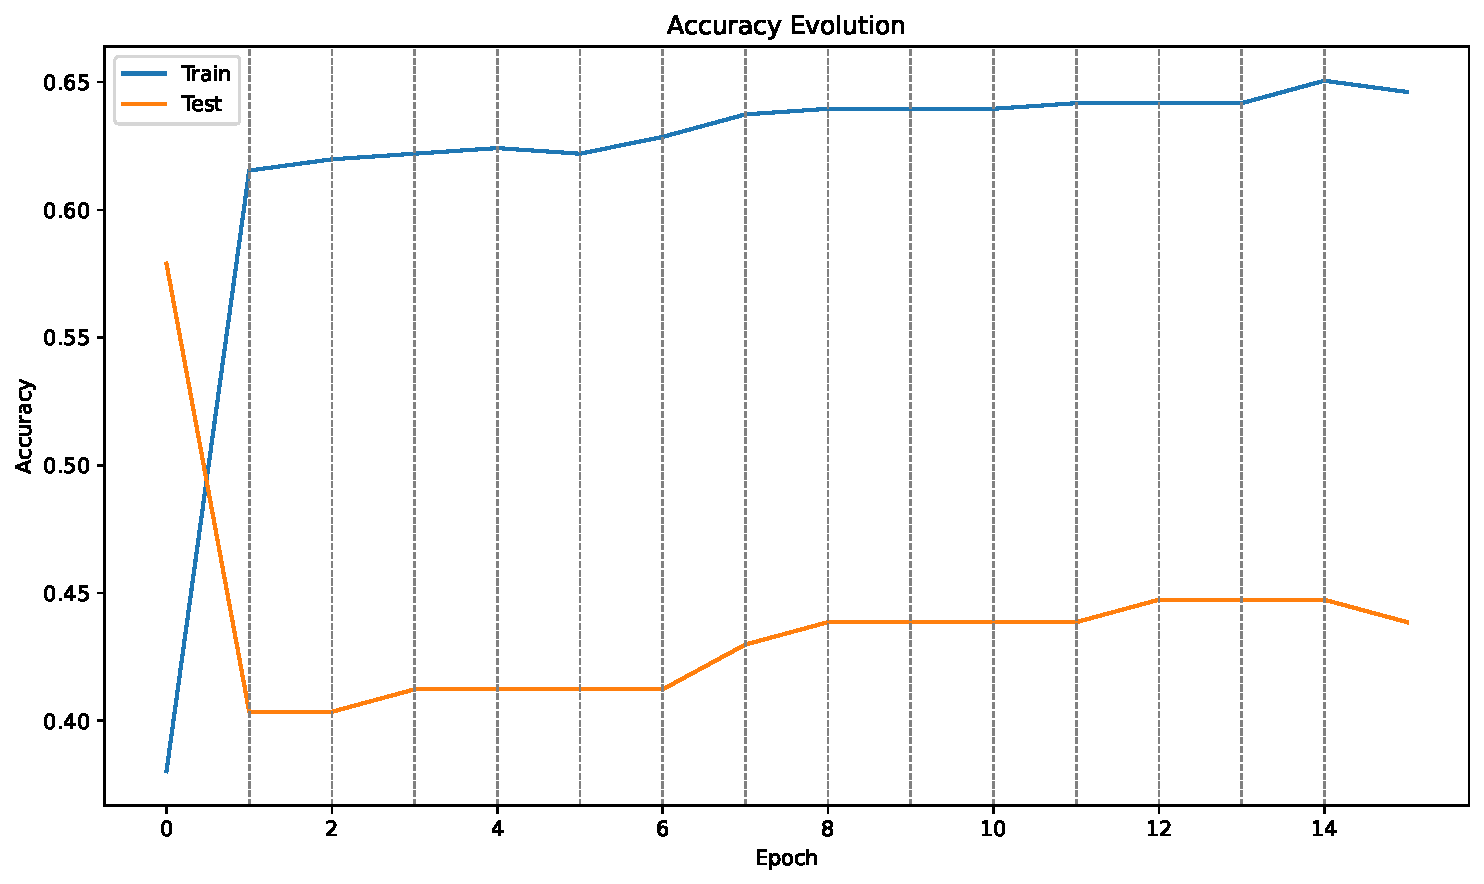
\includegraphics[width=0.3\textwidth]{latex/NN_Train_cancer_16_distrust_trust_PathSize_None__accuracy_evolution.pdf}%
}
\subfloat[{cancer\_16\_distrust\_vacuous}]{%
  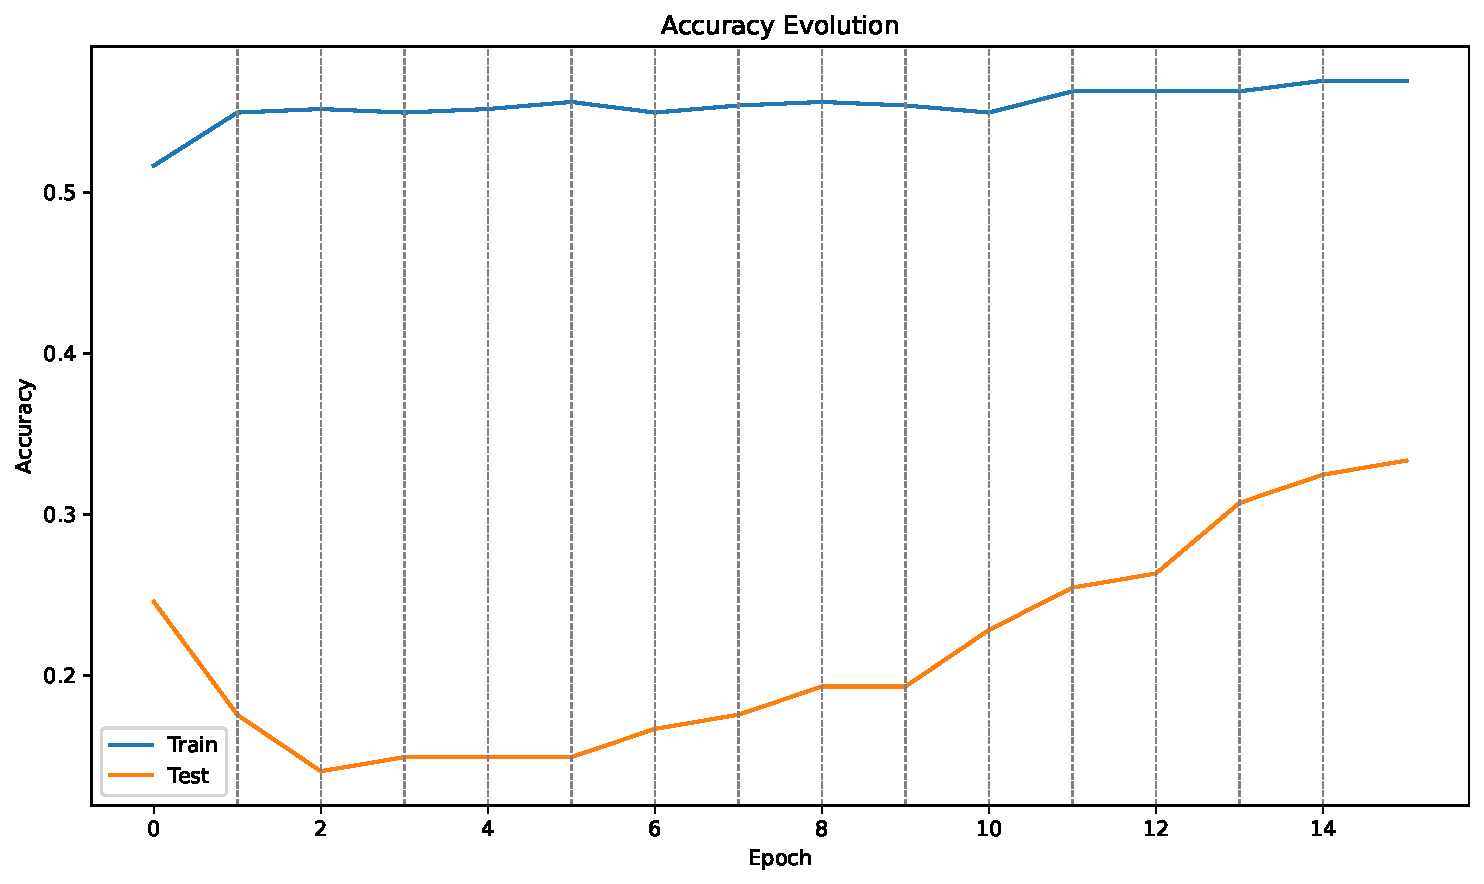
\includegraphics[width=0.3\textwidth]{latex/NN_Train_cancer_16_distrust_vacuous_PathSize_None__accuracy_evolution.pdf}%
}
\subfloat[{cancer\_16\_trust\_distrust}]{%
  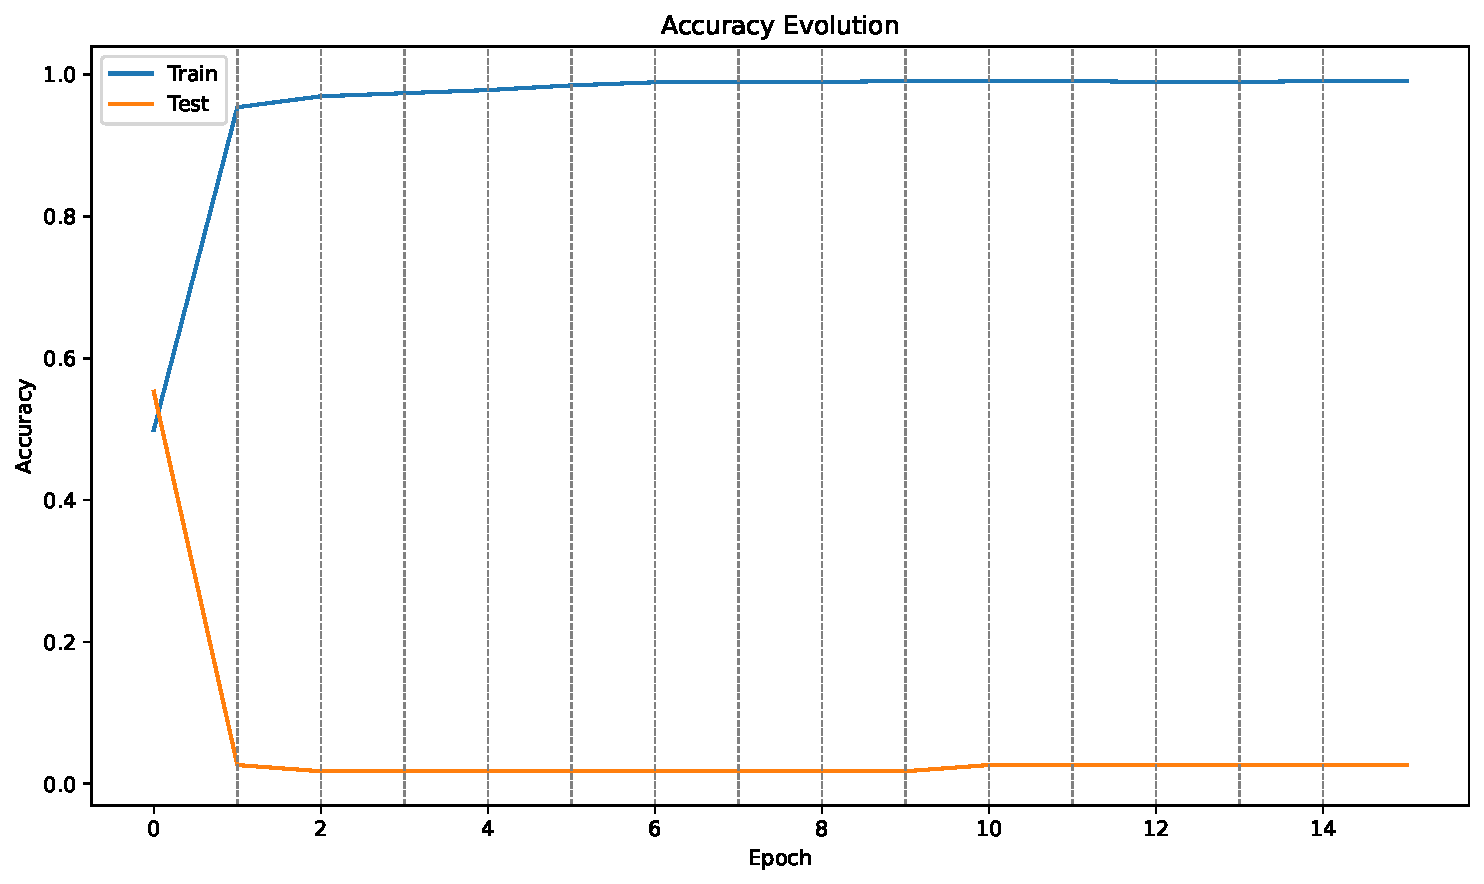
\includegraphics[width=0.3\textwidth]{latex/NN_Train_cancer_16_trust_distrust_PathSize_None__accuracy_evolution.pdf}%
}
\\
\subfloat[{cancer\_16\_trust\_trust}]{%
  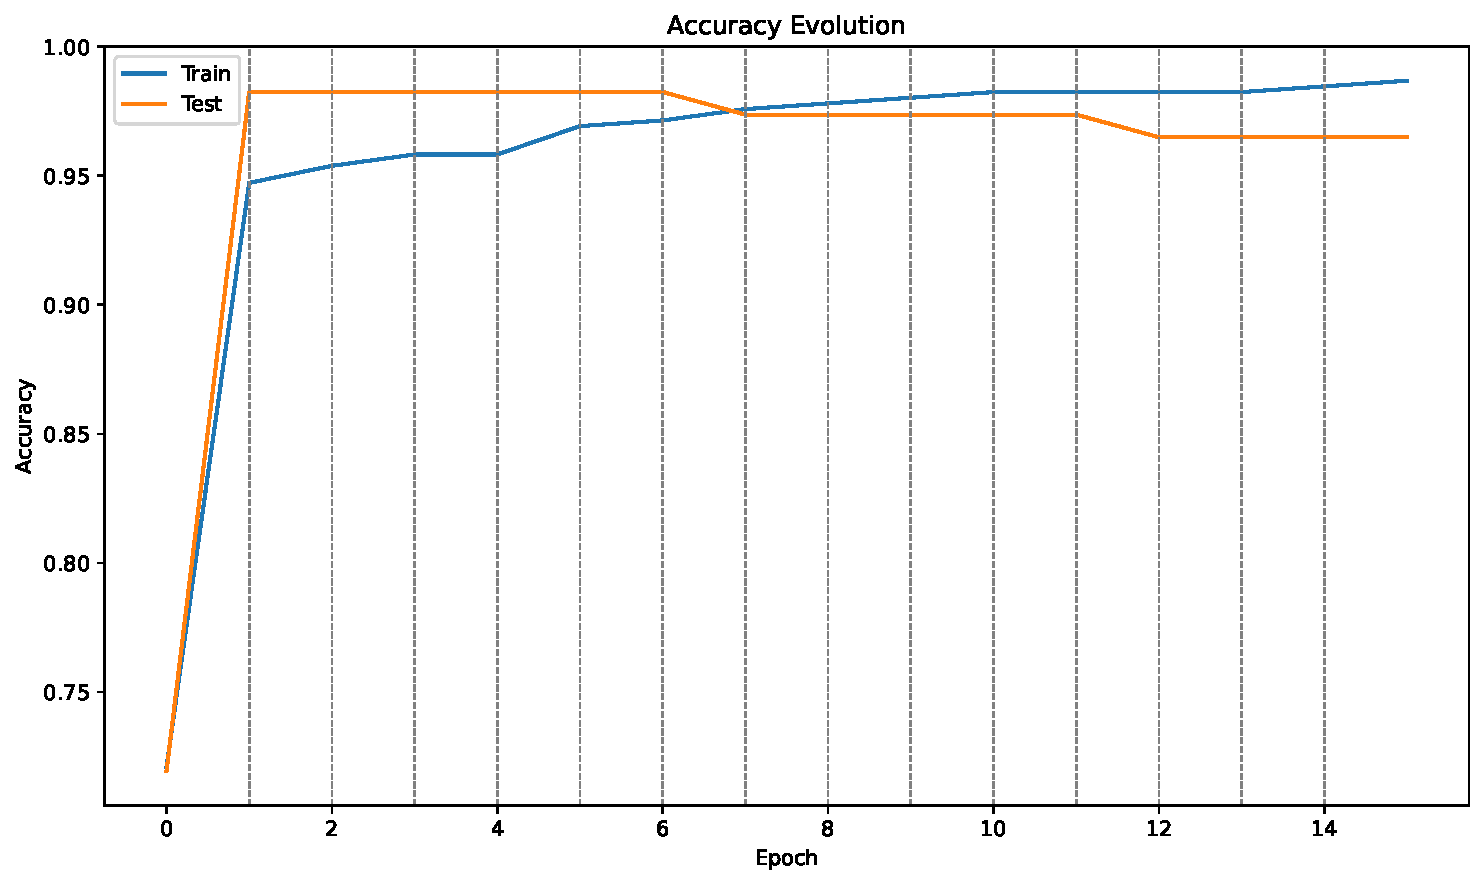
\includegraphics[width=0.3\textwidth]{latex/NN_Train_cancer_16_trust_trust_PathSize_None__accuracy_evolution.pdf}%
}
\subfloat[{cancer\_16\_trust\_vacuous}]{%
  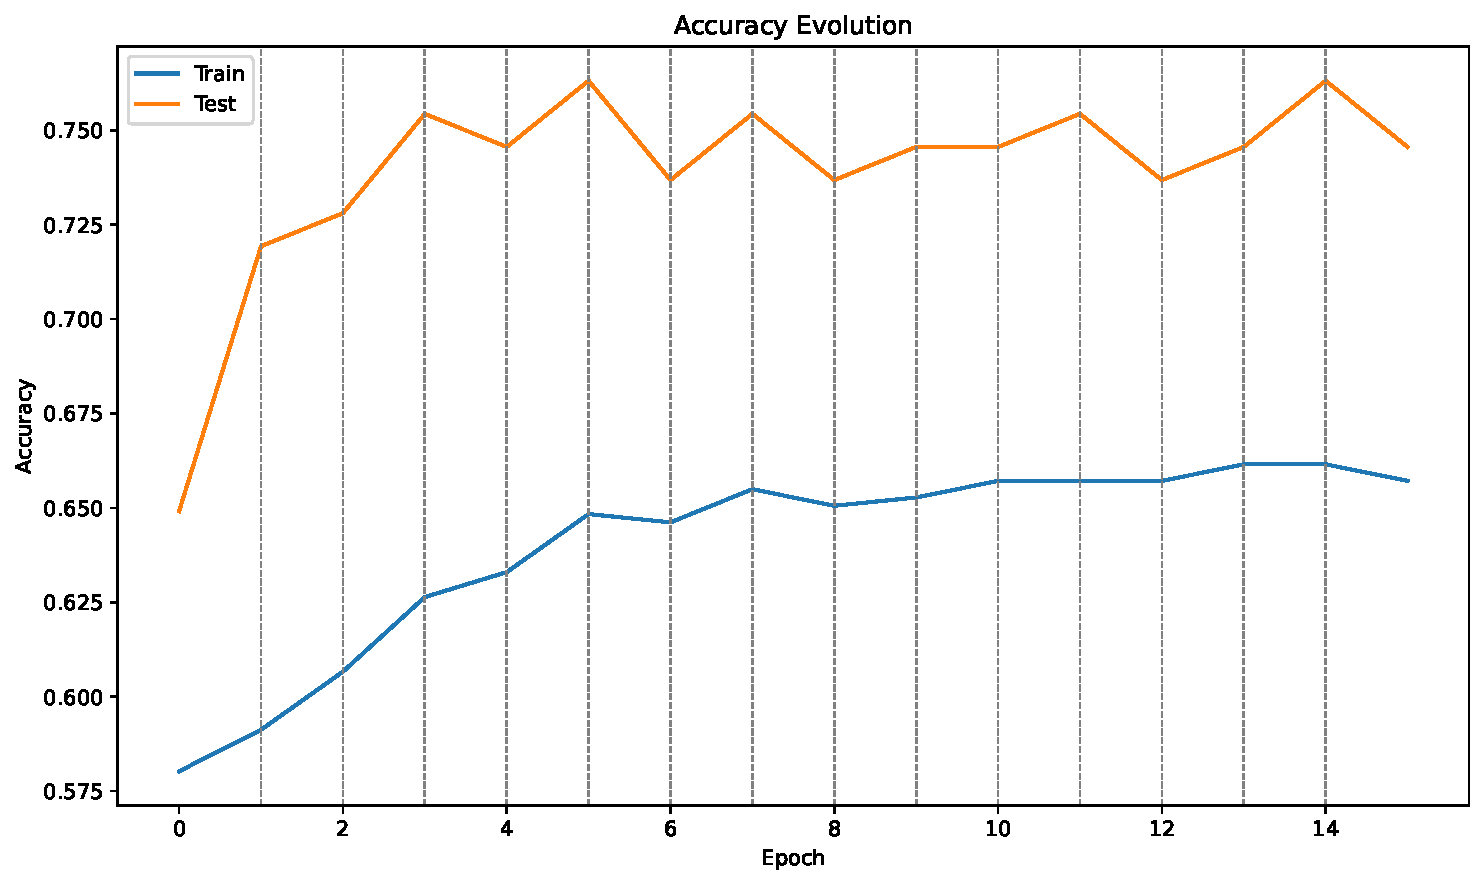
\includegraphics[width=0.3\textwidth]{latex/NN_Train_cancer_16_trust_vacuous_PathSize_None__accuracy_evolution.pdf}%
}
\subfloat[{cancer\_16\_vacuous\_distrust}]{%
  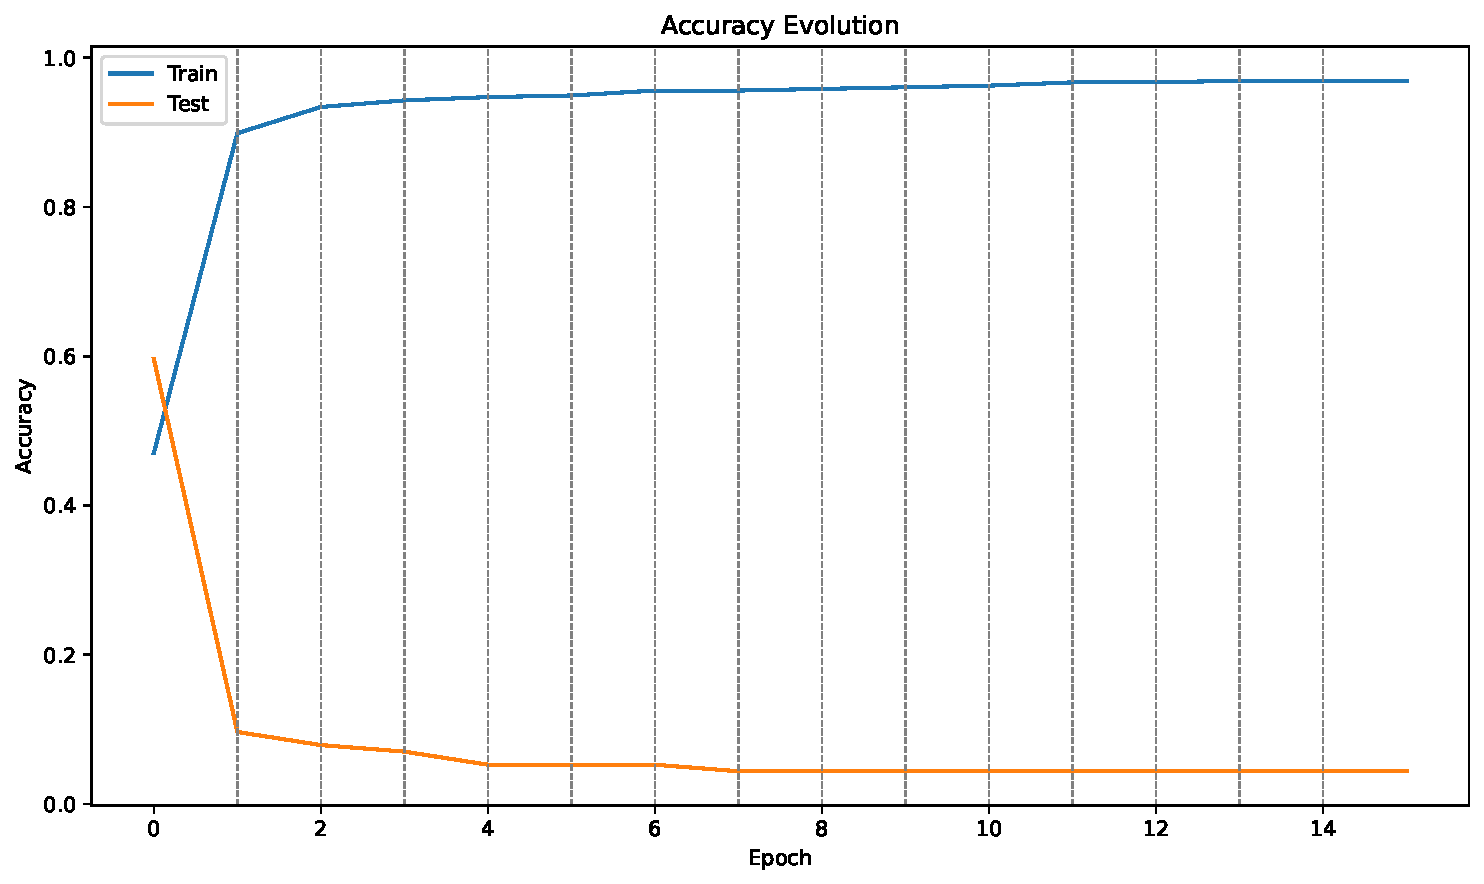
\includegraphics[width=0.3\textwidth]{latex/NN_Train_cancer_16_vacuous_distrust_PathSize_None__accuracy_evolution.pdf}%
}
\endgroup
\\
\caption{Accuracy Evolution (1/3)}
\end{figure}

\begin{figure}[htbp]
\centering
\begingroup
\captionsetup[subfloat]{justification=centering,singlelinecheck=false, font=scriptsize}
\subfloat[{cancer\_16\_vacuous\_trust}]{%
  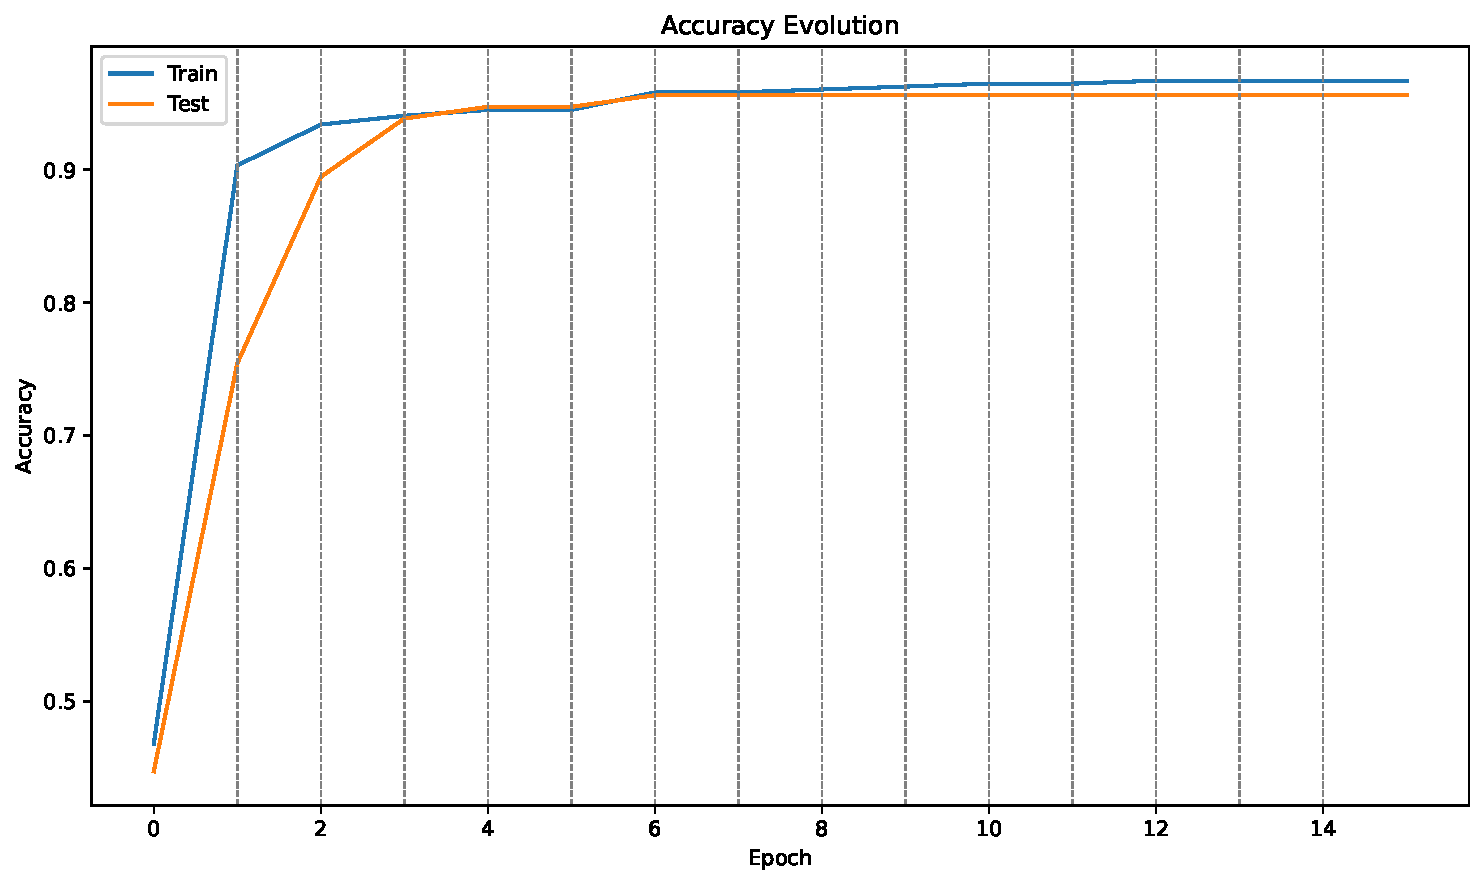
\includegraphics[width=0.3\textwidth]{latex/NN_Train_cancer_16_vacuous_trust_PathSize_None__accuracy_evolution.pdf}%
}
\subfloat[{cancer\_16\_vacuous\_vacuous}]{%
  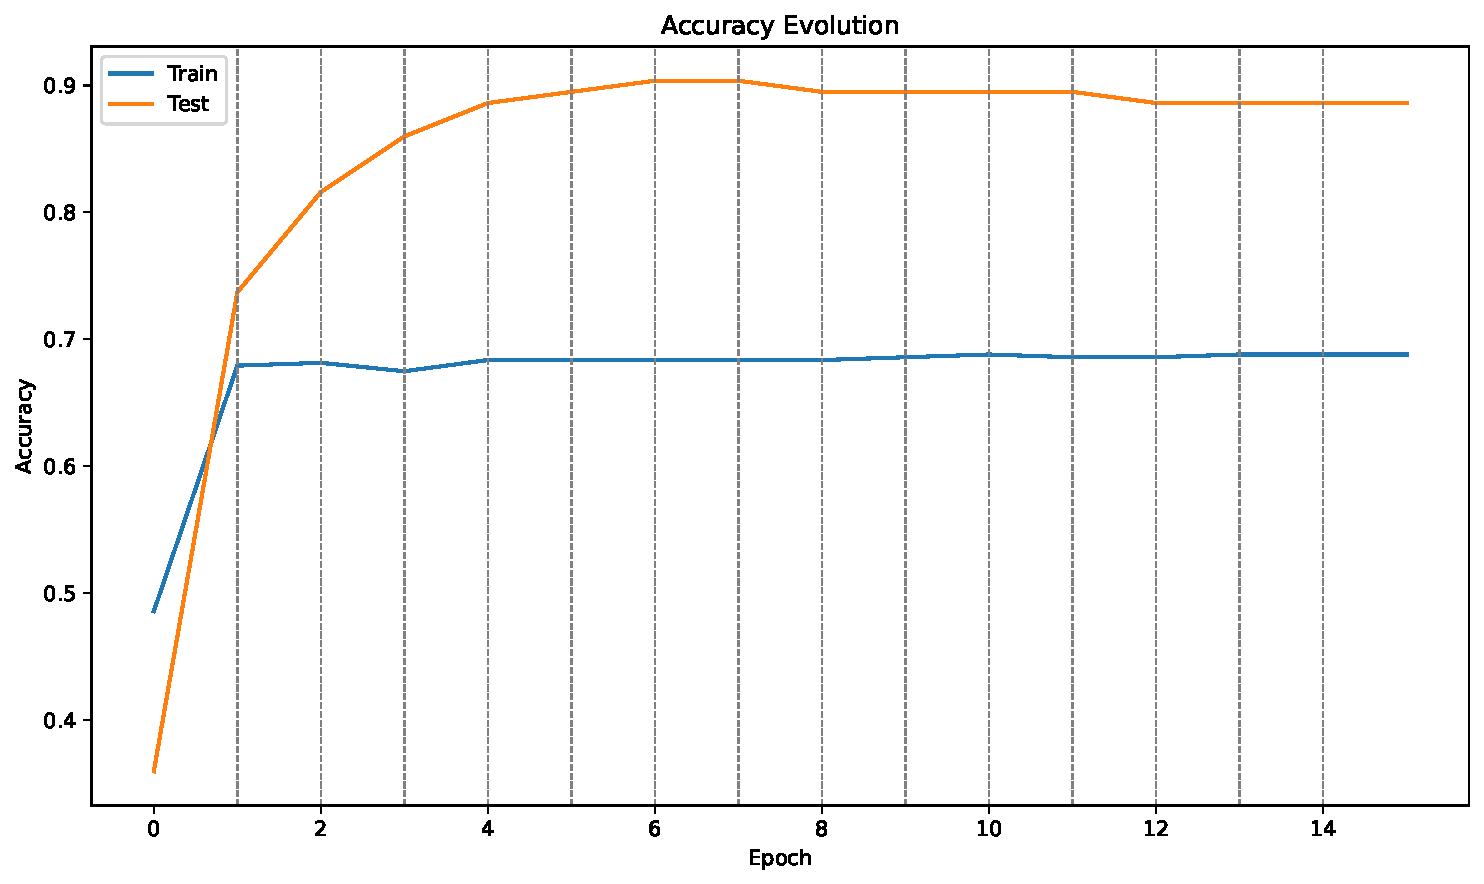
\includegraphics[width=0.3\textwidth]{latex/NN_Train_cancer_16_vacuous_vacuous_PathSize_None__accuracy_evolution.pdf}%
}
\subfloat[{mnist\_128\_trust\_trust, ps=1}]{%
  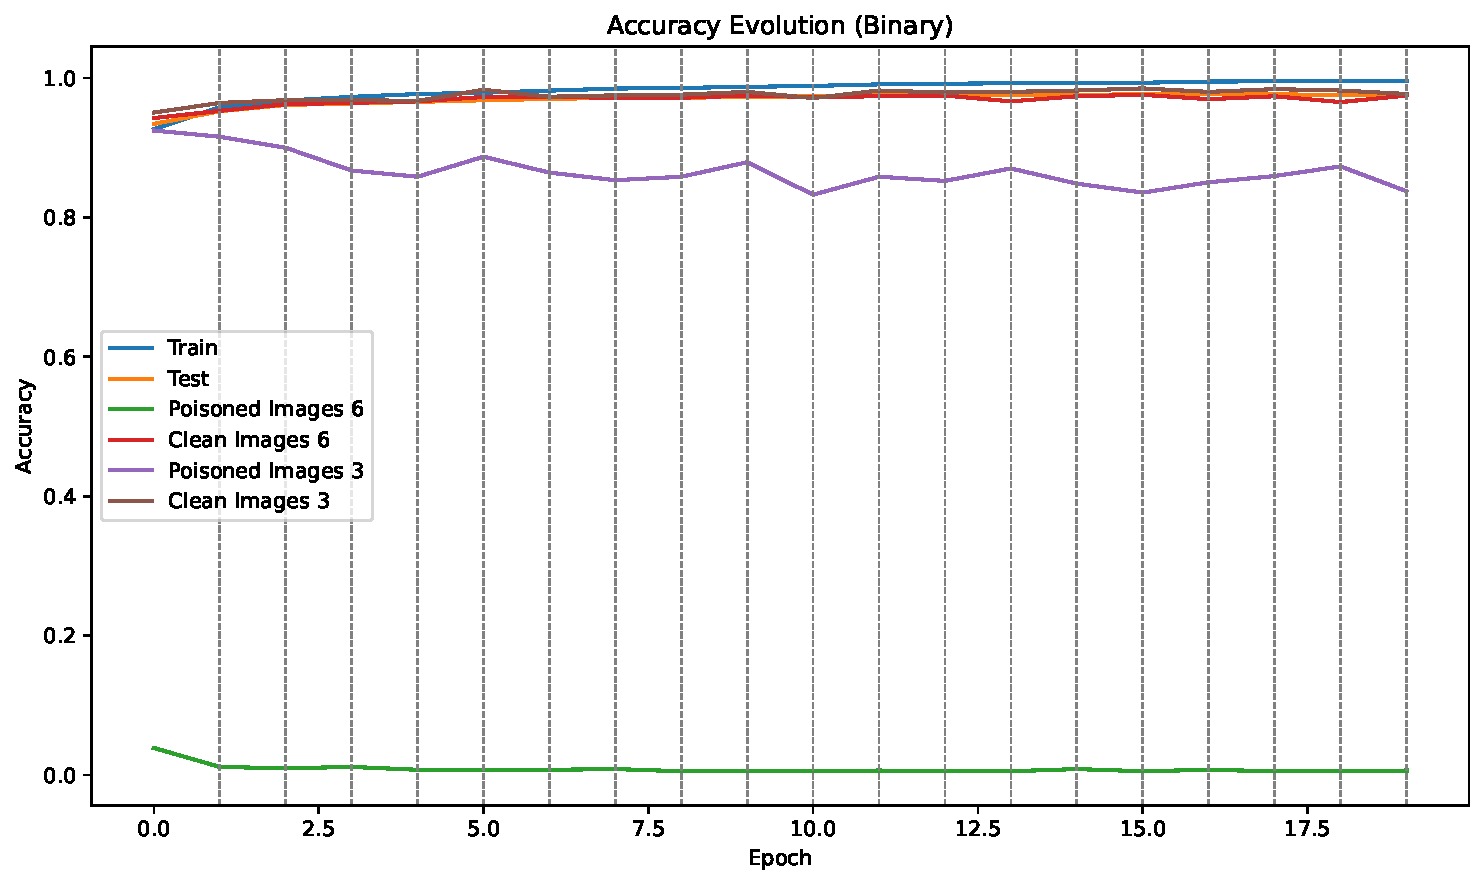
\includegraphics[width=0.3\textwidth]{latex/NN_Train_mnist_128_trust_trust_PathSize_1__accuracy_evolution.pdf}%
}
\\
\subfloat[{mnist\_128\_trust\_trust, ps=10}]{%
  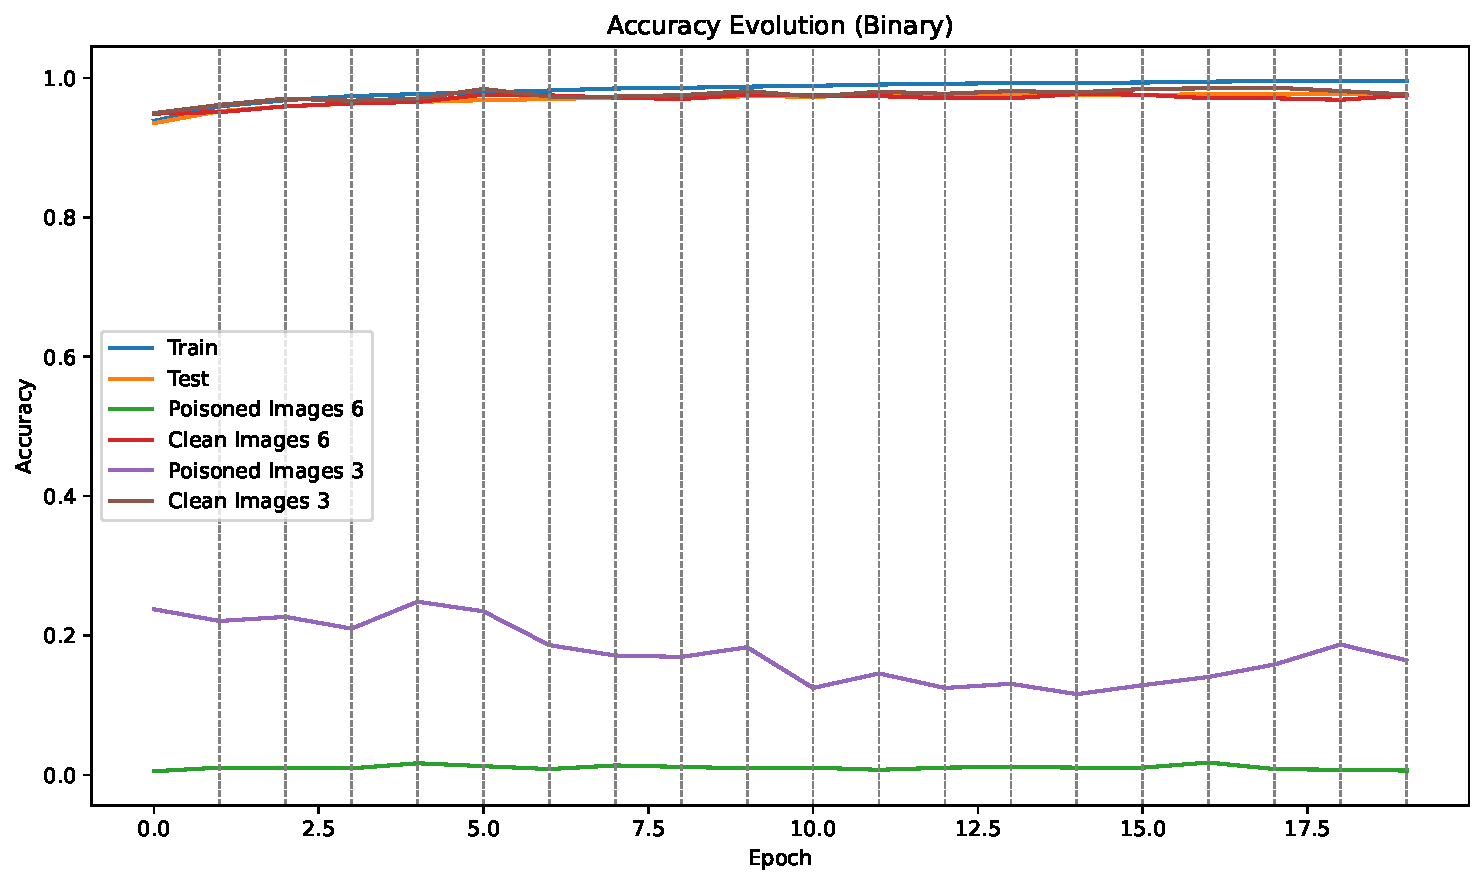
\includegraphics[width=0.3\textwidth]{latex/NN_Train_mnist_128_trust_trust_PathSize_10__accuracy_evolution.pdf}%
}
\subfloat[{mnist\_128\_trust\_trust, ps=27}]{%
  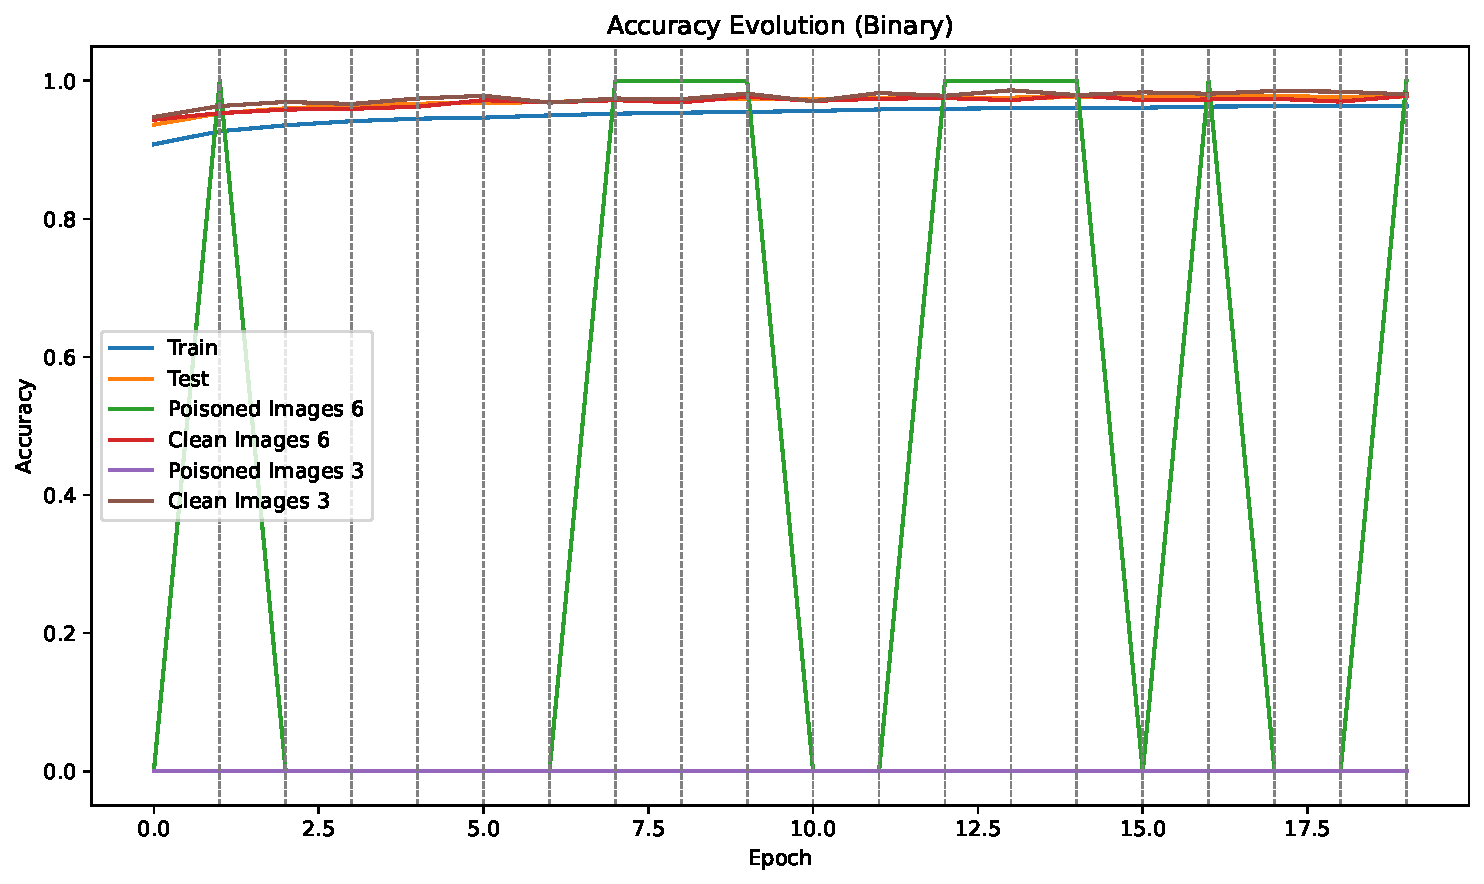
\includegraphics[width=0.3\textwidth]{latex/NN_Train_mnist_128_trust_trust_PathSize_27__accuracy_evolution.pdf}%
}
\subfloat[{mnist\_128\_trust\_trust, ps=4}]{%
  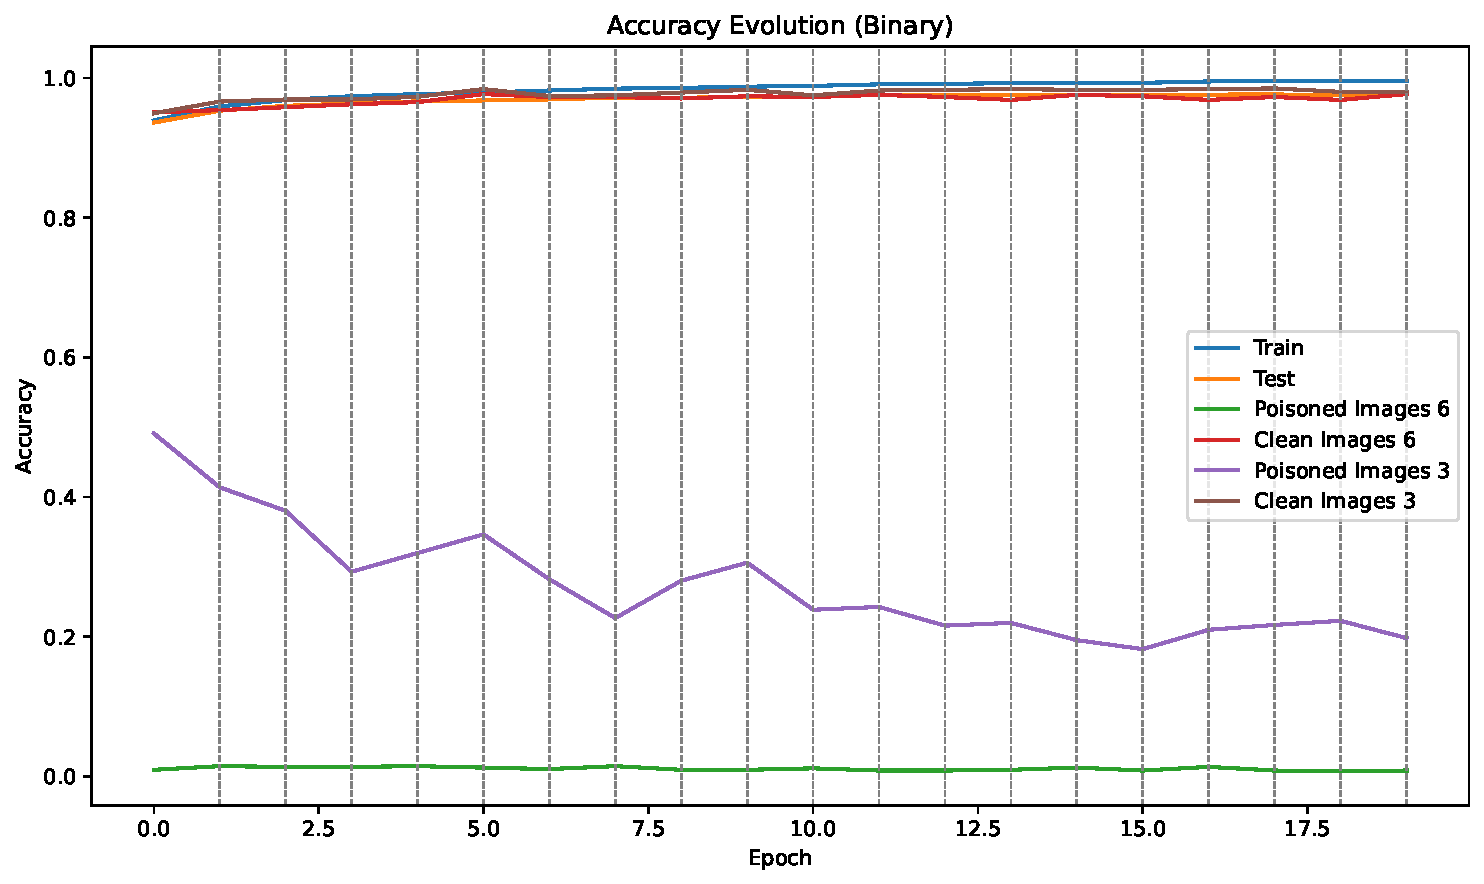
\includegraphics[width=0.3\textwidth]{latex/NN_Train_mnist_128_trust_trust_PathSize_4__accuracy_evolution.pdf}%
}
\\
\subfloat[{mnist\_128\_vacuous\_vacuous}]{%
  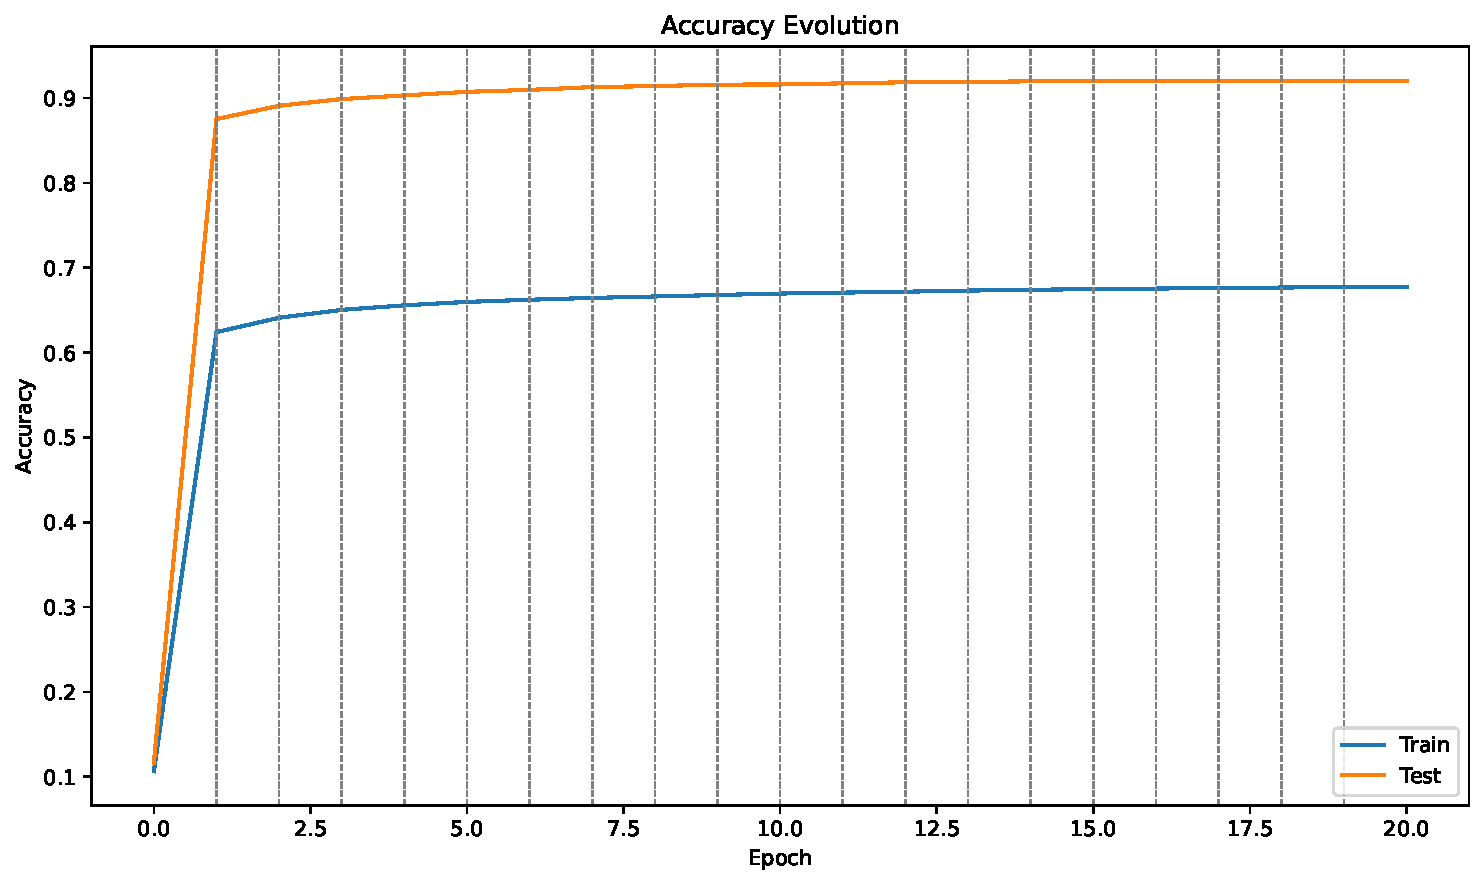
\includegraphics[width=0.3\textwidth]{latex/NN_Train_mnist_128_vacuous_vacuous_PathSize_None__accuracy_evolution.pdf}%
}
\subfloat[{mnist\_16\_16\_trust\_trust}]{%
  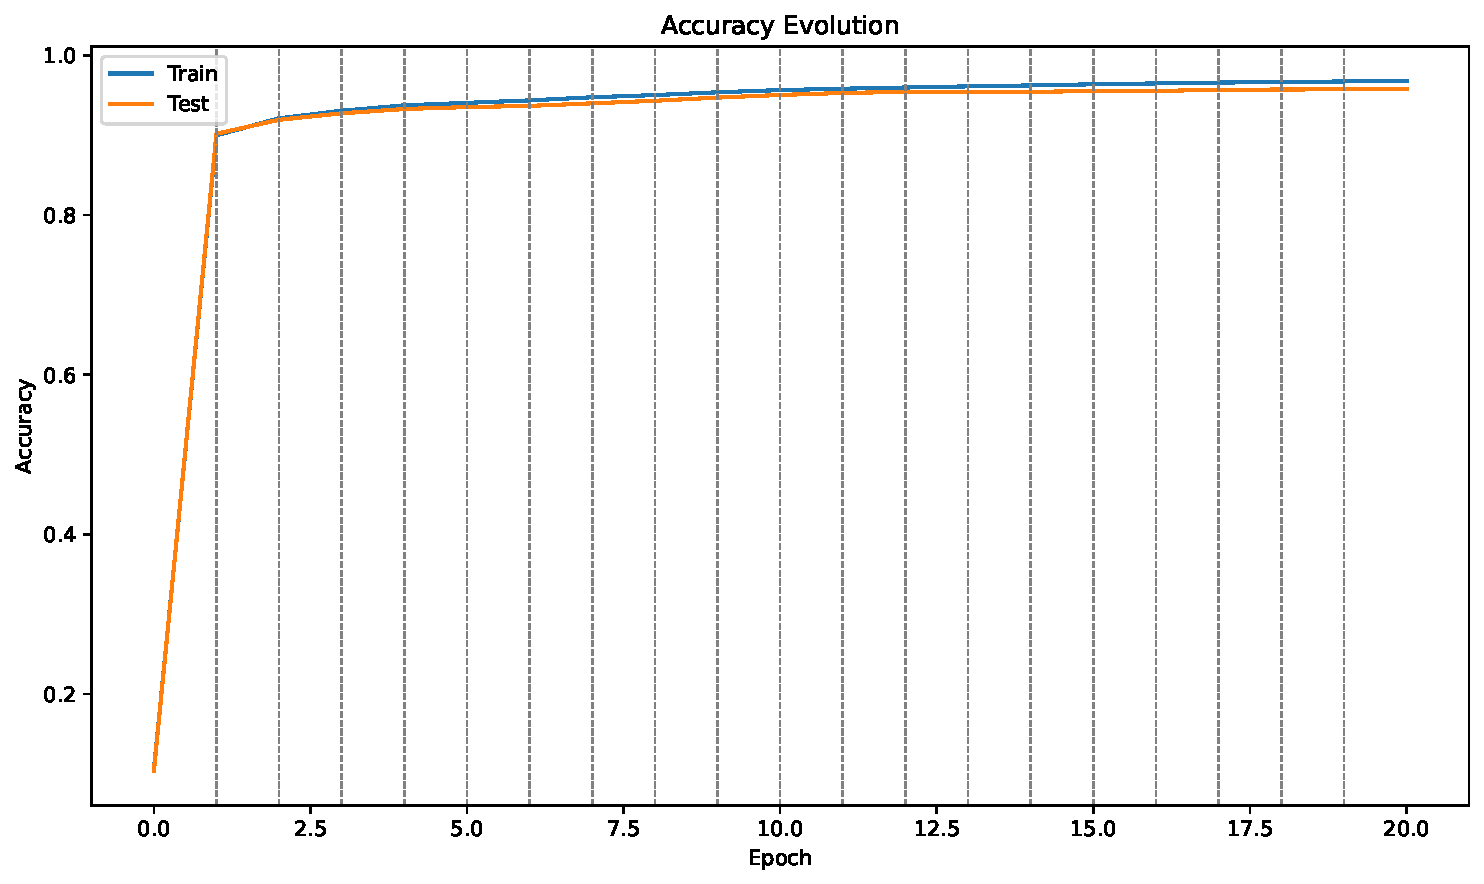
\includegraphics[width=0.3\textwidth]{latex/NN_Train_mnist_16_16_trust_trust_PathSize_None__accuracy_evolution.pdf}%
}
\subfloat[{mnist\_16\_16\_vacuous\_vacuous}]{%
  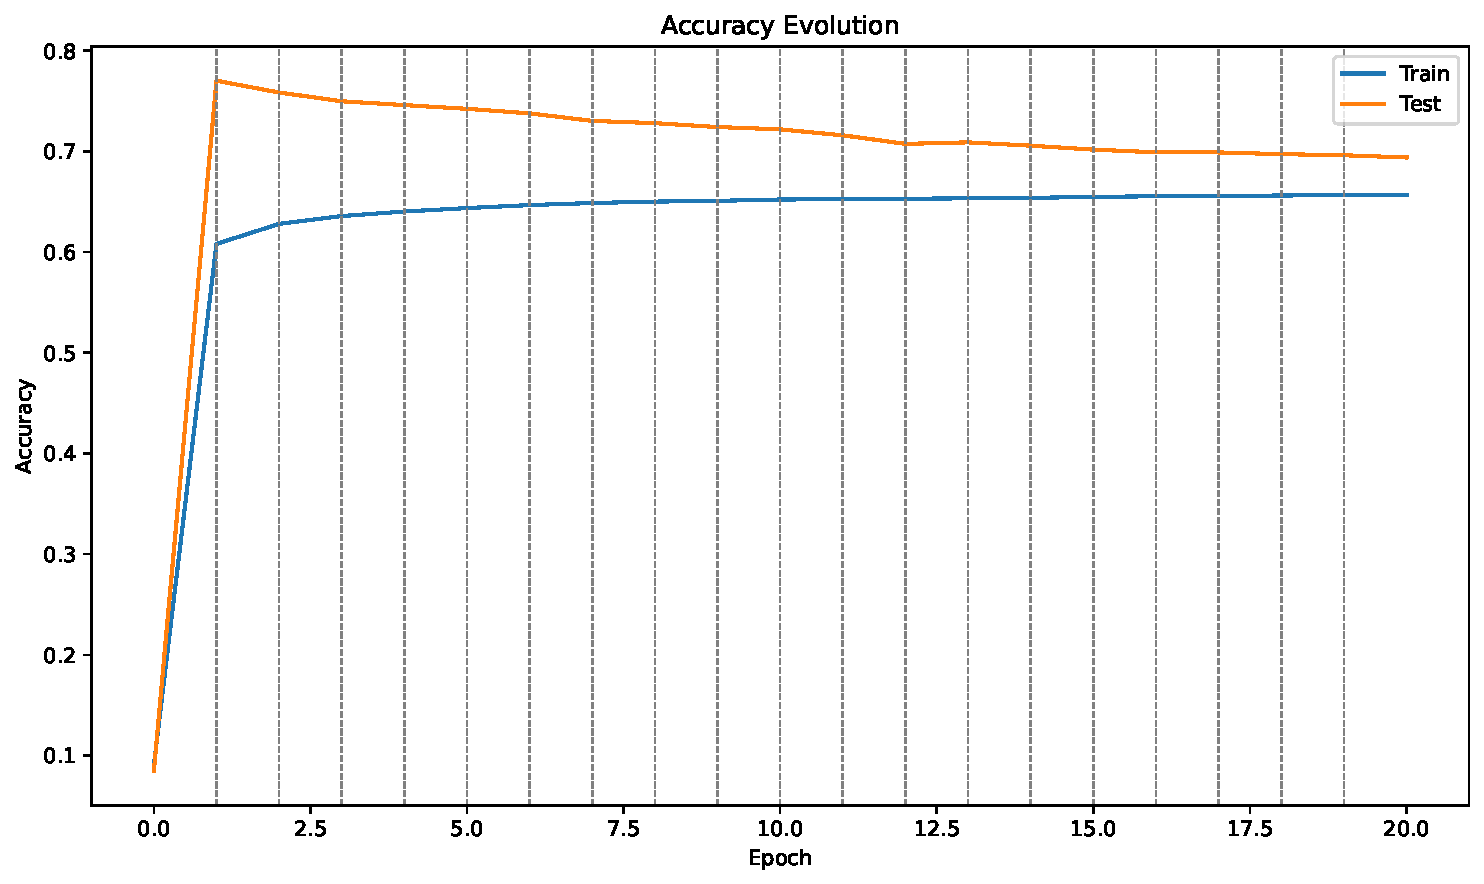
\includegraphics[width=0.3\textwidth]{latex/NN_Train_mnist_16_16_vacuous_vacuous_PathSize_None__accuracy_evolution.pdf}%
}
\endgroup
\\
\caption{Accuracy Evolution (2/3)}
\end{figure}

\begin{figure}[htbp]
\centering
\begingroup
\captionsetup[subfloat]{justification=centering,singlelinecheck=false, font=scriptsize}
\subfloat[{mnist\_16\_trust\_trust}]{%
  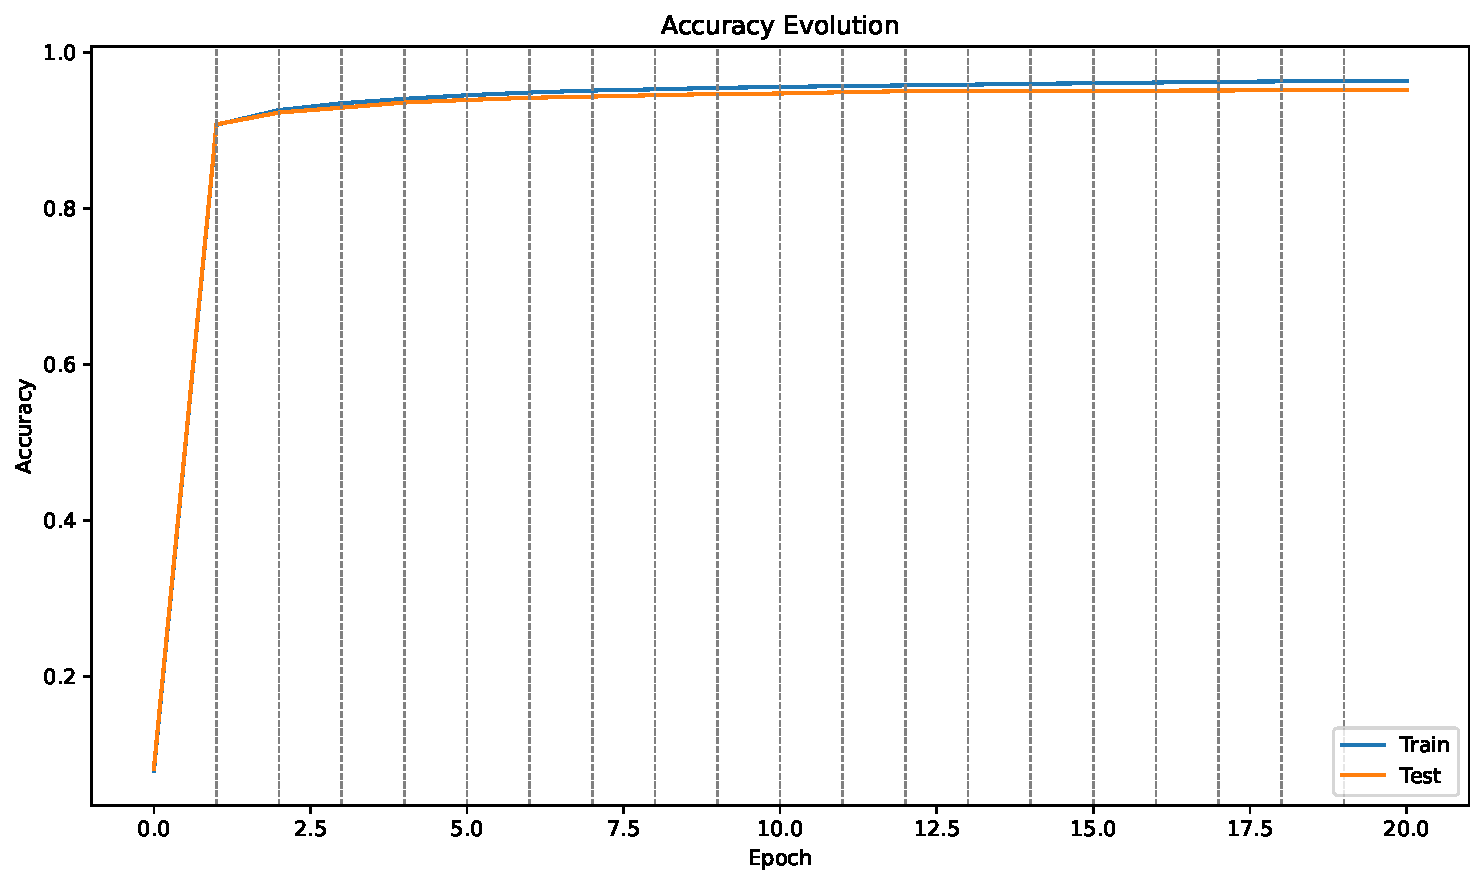
\includegraphics[width=0.3\textwidth]{latex/NN_Train_mnist_16_trust_trust_PathSize_None__accuracy_evolution.pdf}%
}
\subfloat[{mnist\_16\_vacuous\_vacuous}]{%
  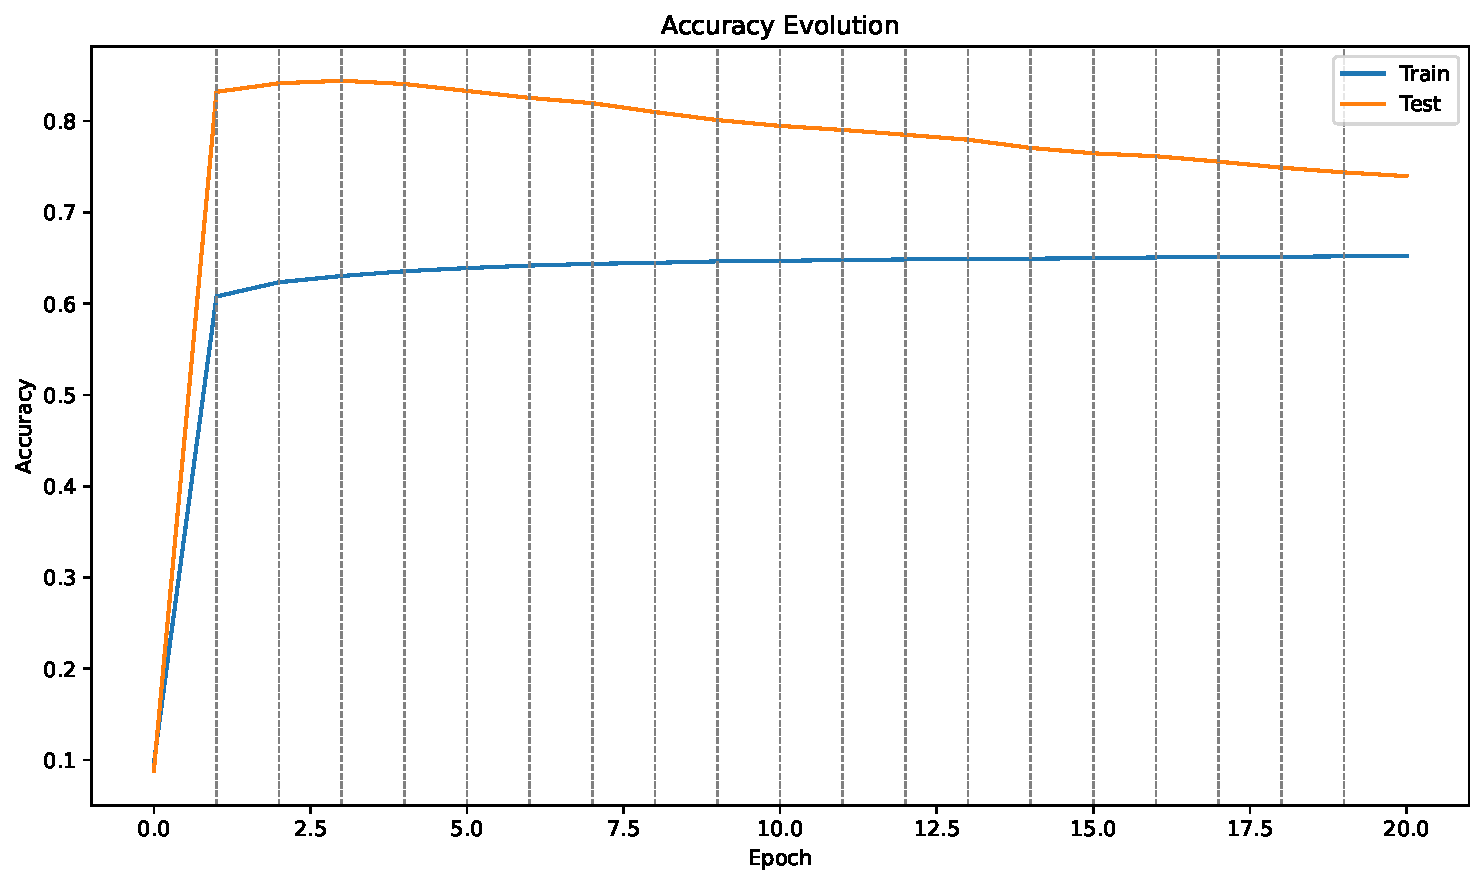
\includegraphics[width=0.3\textwidth]{latex/NN_Train_mnist_16_vacuous_vacuous_PathSize_None__accuracy_evolution.pdf}%
}
\subfloat[{mnist\_32\_vacuous\_vacuous}]{%
  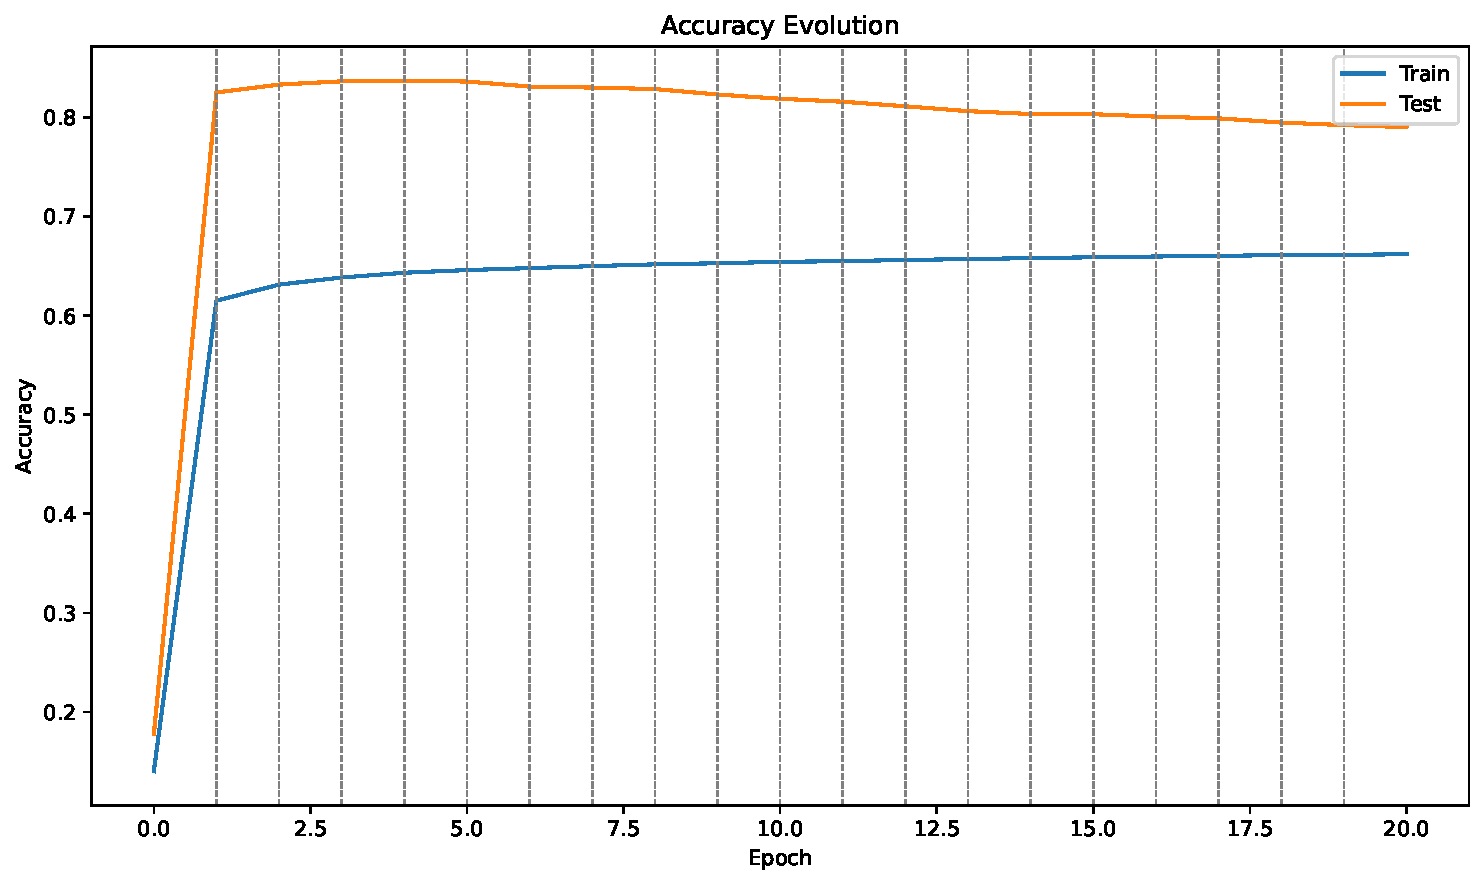
\includegraphics[width=0.3\textwidth]{latex/NN_Train_mnist_32_vacuous_vacuous_PathSize_None__accuracy_evolution.pdf}%
}
\\
\subfloat[{mnist\_64\_vacuous\_vacuous}]{%
  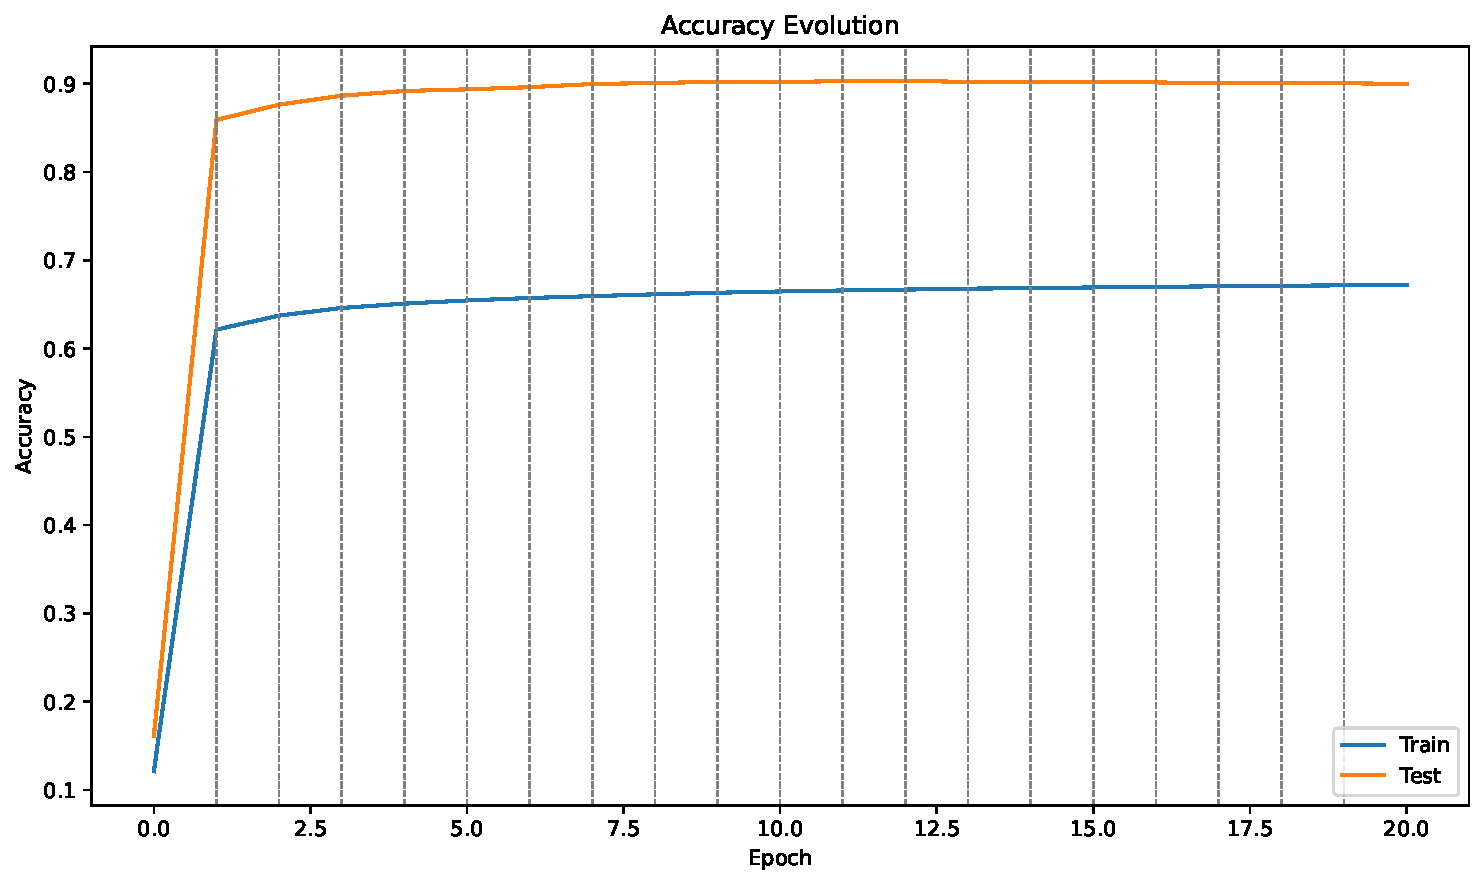
\includegraphics[width=0.3\textwidth]{latex/NN_Train_mnist_64_vacuous_vacuous_PathSize_None__accuracy_evolution.pdf}%
}
\endgroup
\caption{Accuracy Evolution (3/3)}
\end{figure}


\section{\acs{PaTAS} Evaluation Results}

\subsection{Cancer Dataset}

\subsubsection{(0.25, 0.0, 0.75) -- (0.25, 0.0, 0.75)}

\begin{figure}[htbp]
\centering
  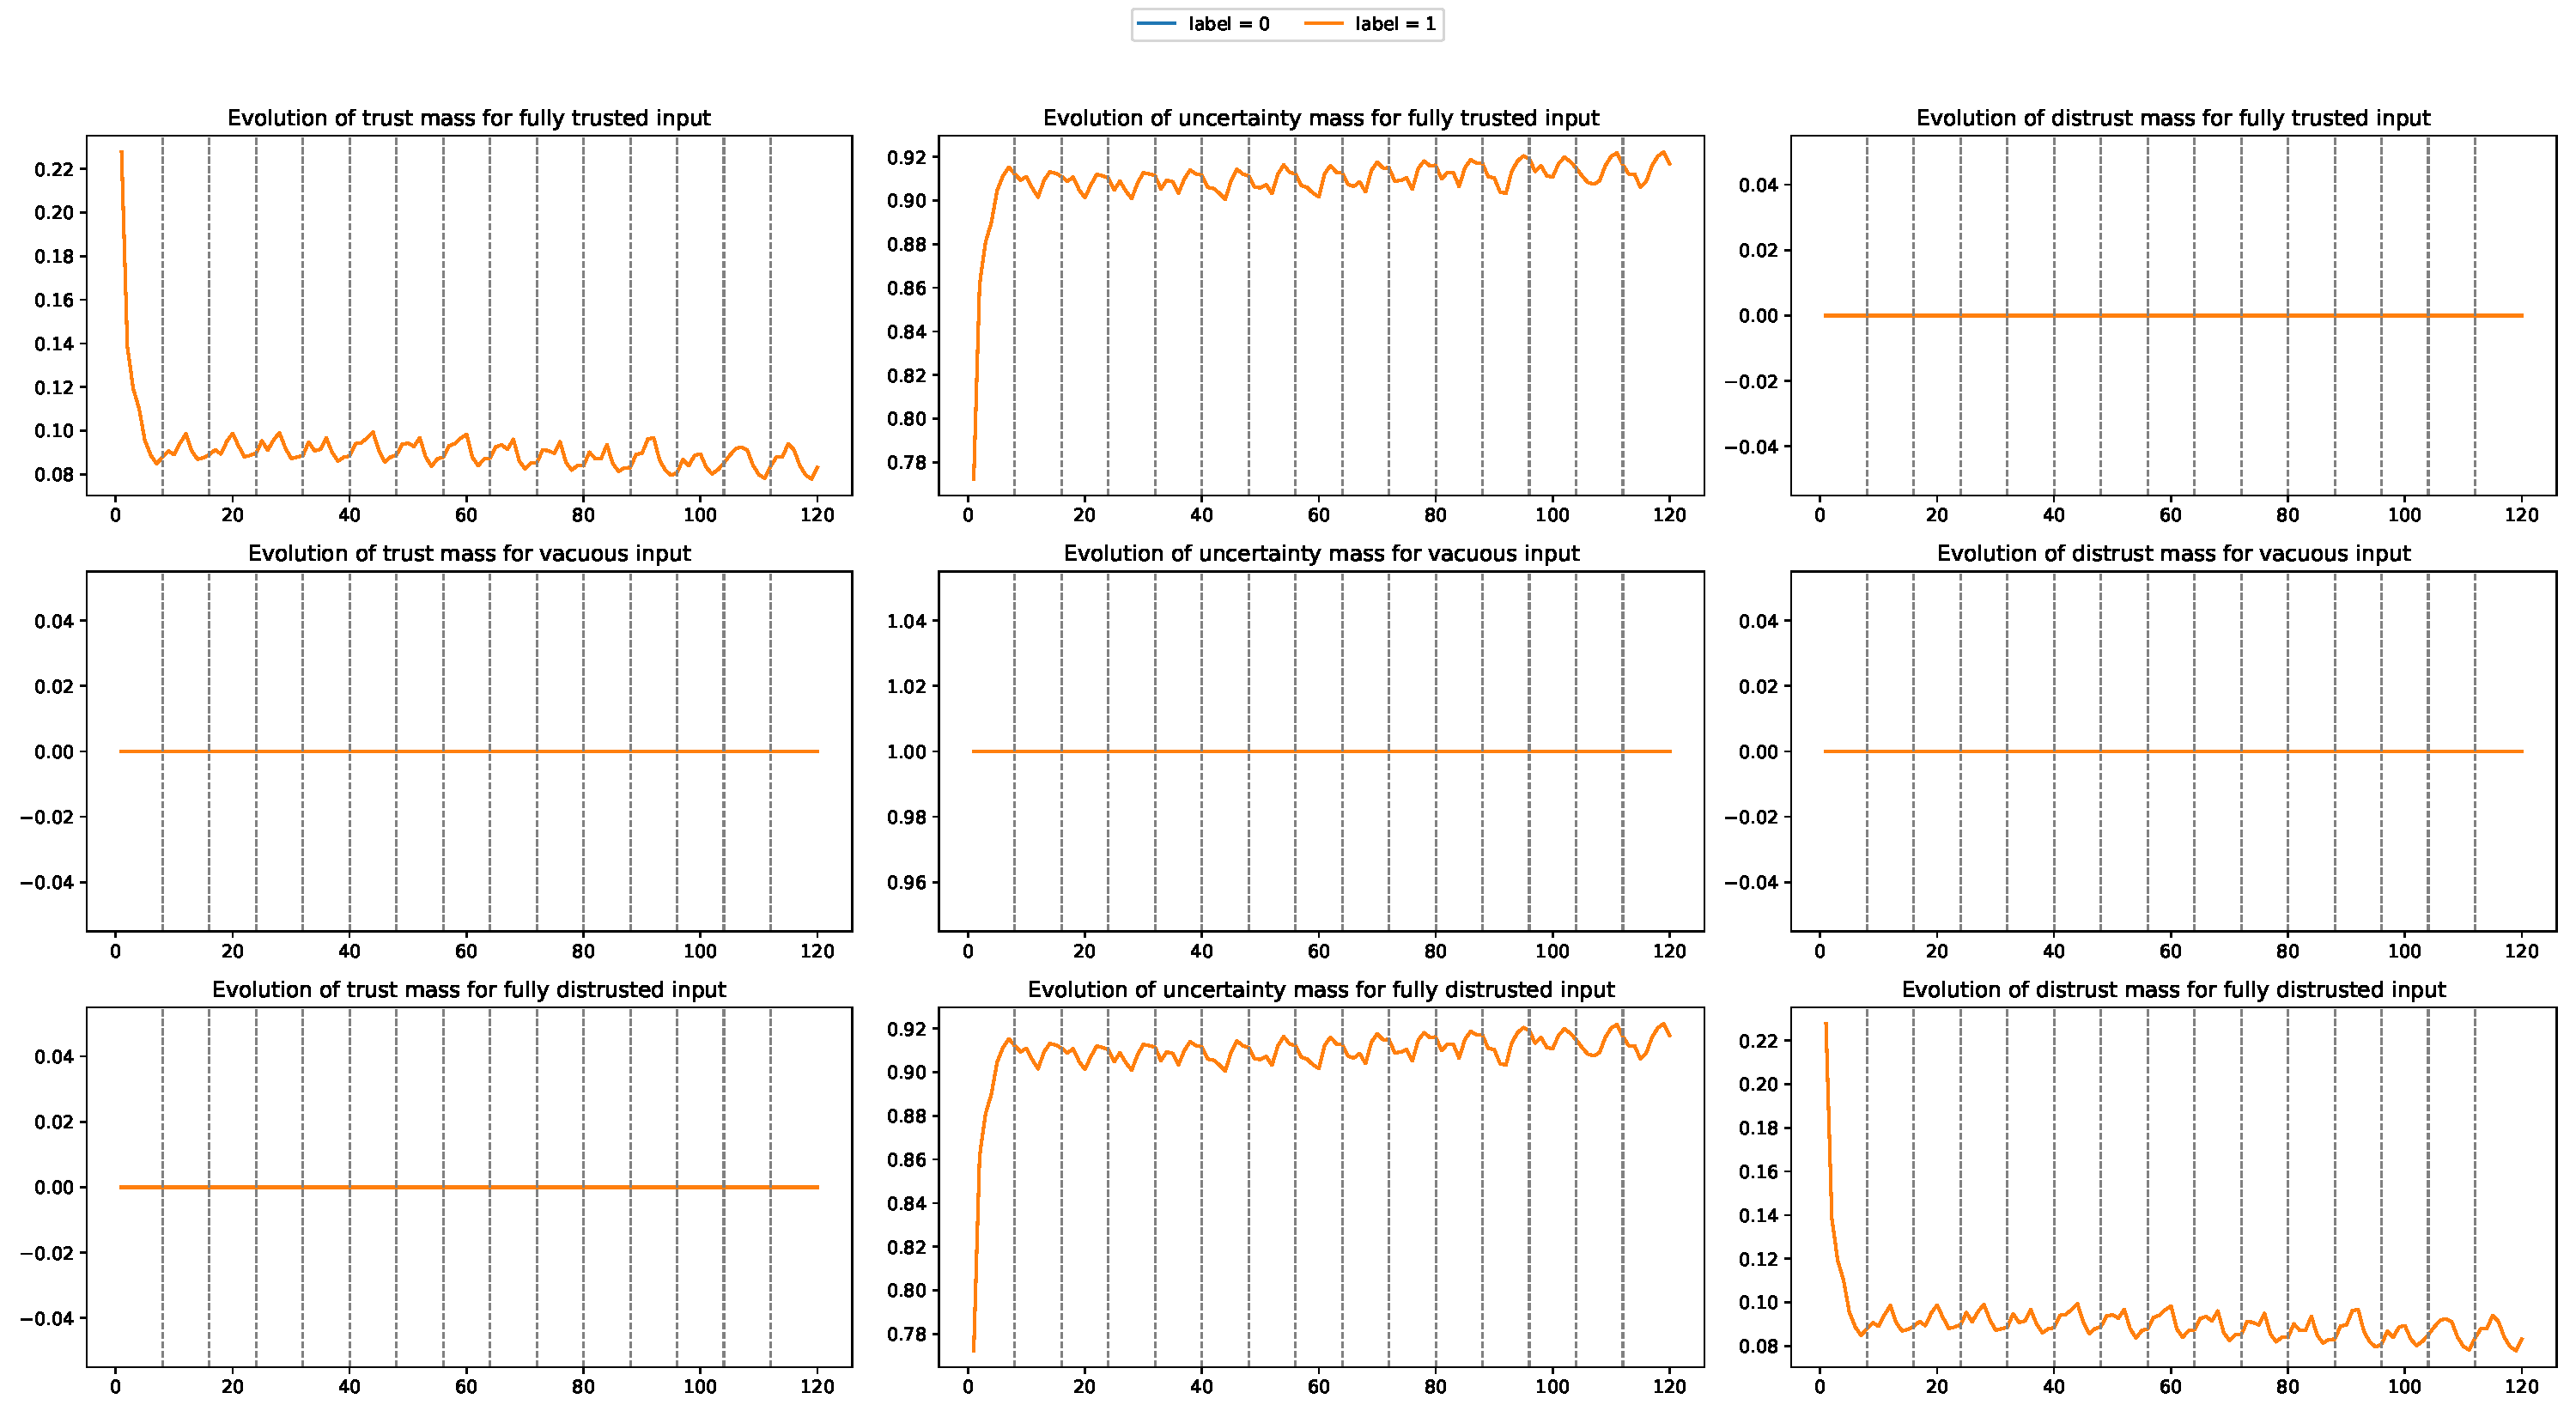
\includegraphics[width=0.8\textwidth]{latex/PTAS_Eval_cancer_16_0.25_0.0_0.75_0.25_0.0_0.75_eps_0.001_PathSize_None__plot_ptas.pdf}
\caption{cancer\_16\_0.25,0.0,0.75\_0.25,0.0,0.75, $\varepsilon$=0.001}
\end{figure}

\begin{figure}[htbp]
\centering
  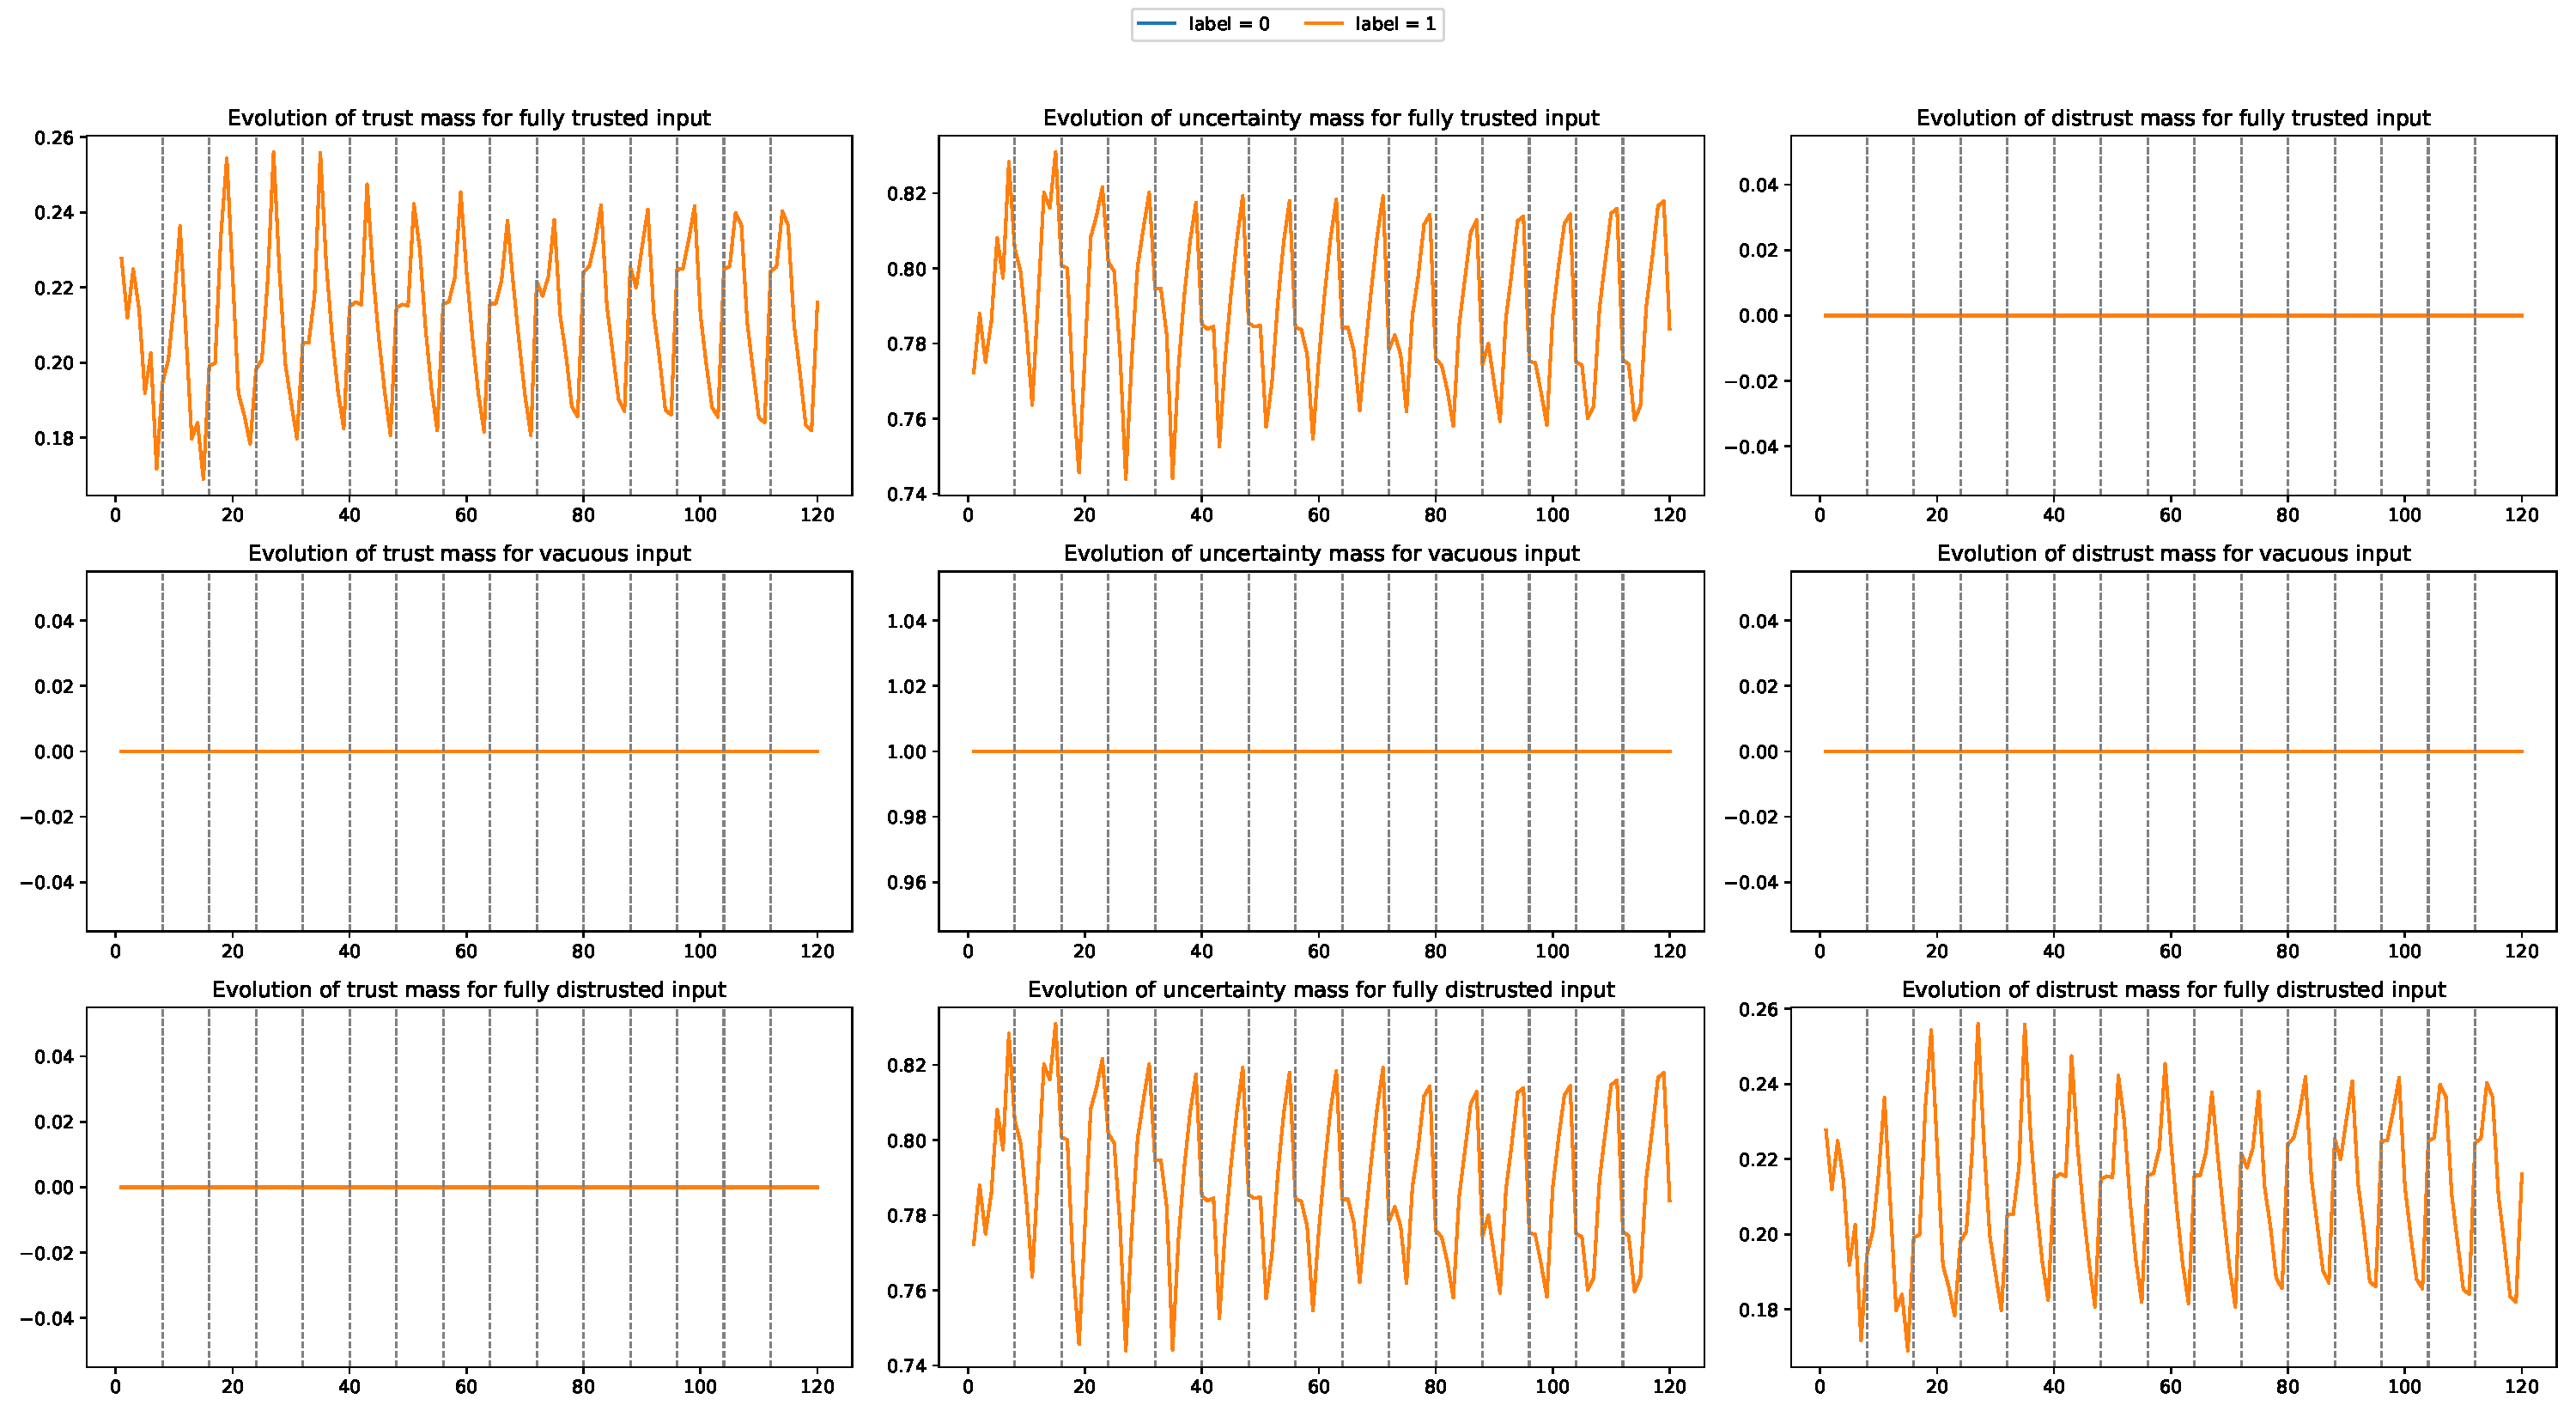
\includegraphics[width=0.8\textwidth]{latex/PTAS_Eval_cancer_16_0.25_0.0_0.75_0.25_0.0_0.75_eps_0.01_PathSize_None__plot_ptas.pdf}
\caption{cancer\_16\_0.25,0.0,0.75\_0.25,0.0,0.75, $\varepsilon$=0.01}
\end{figure}

\begin{figure}[htbp]
\centering
  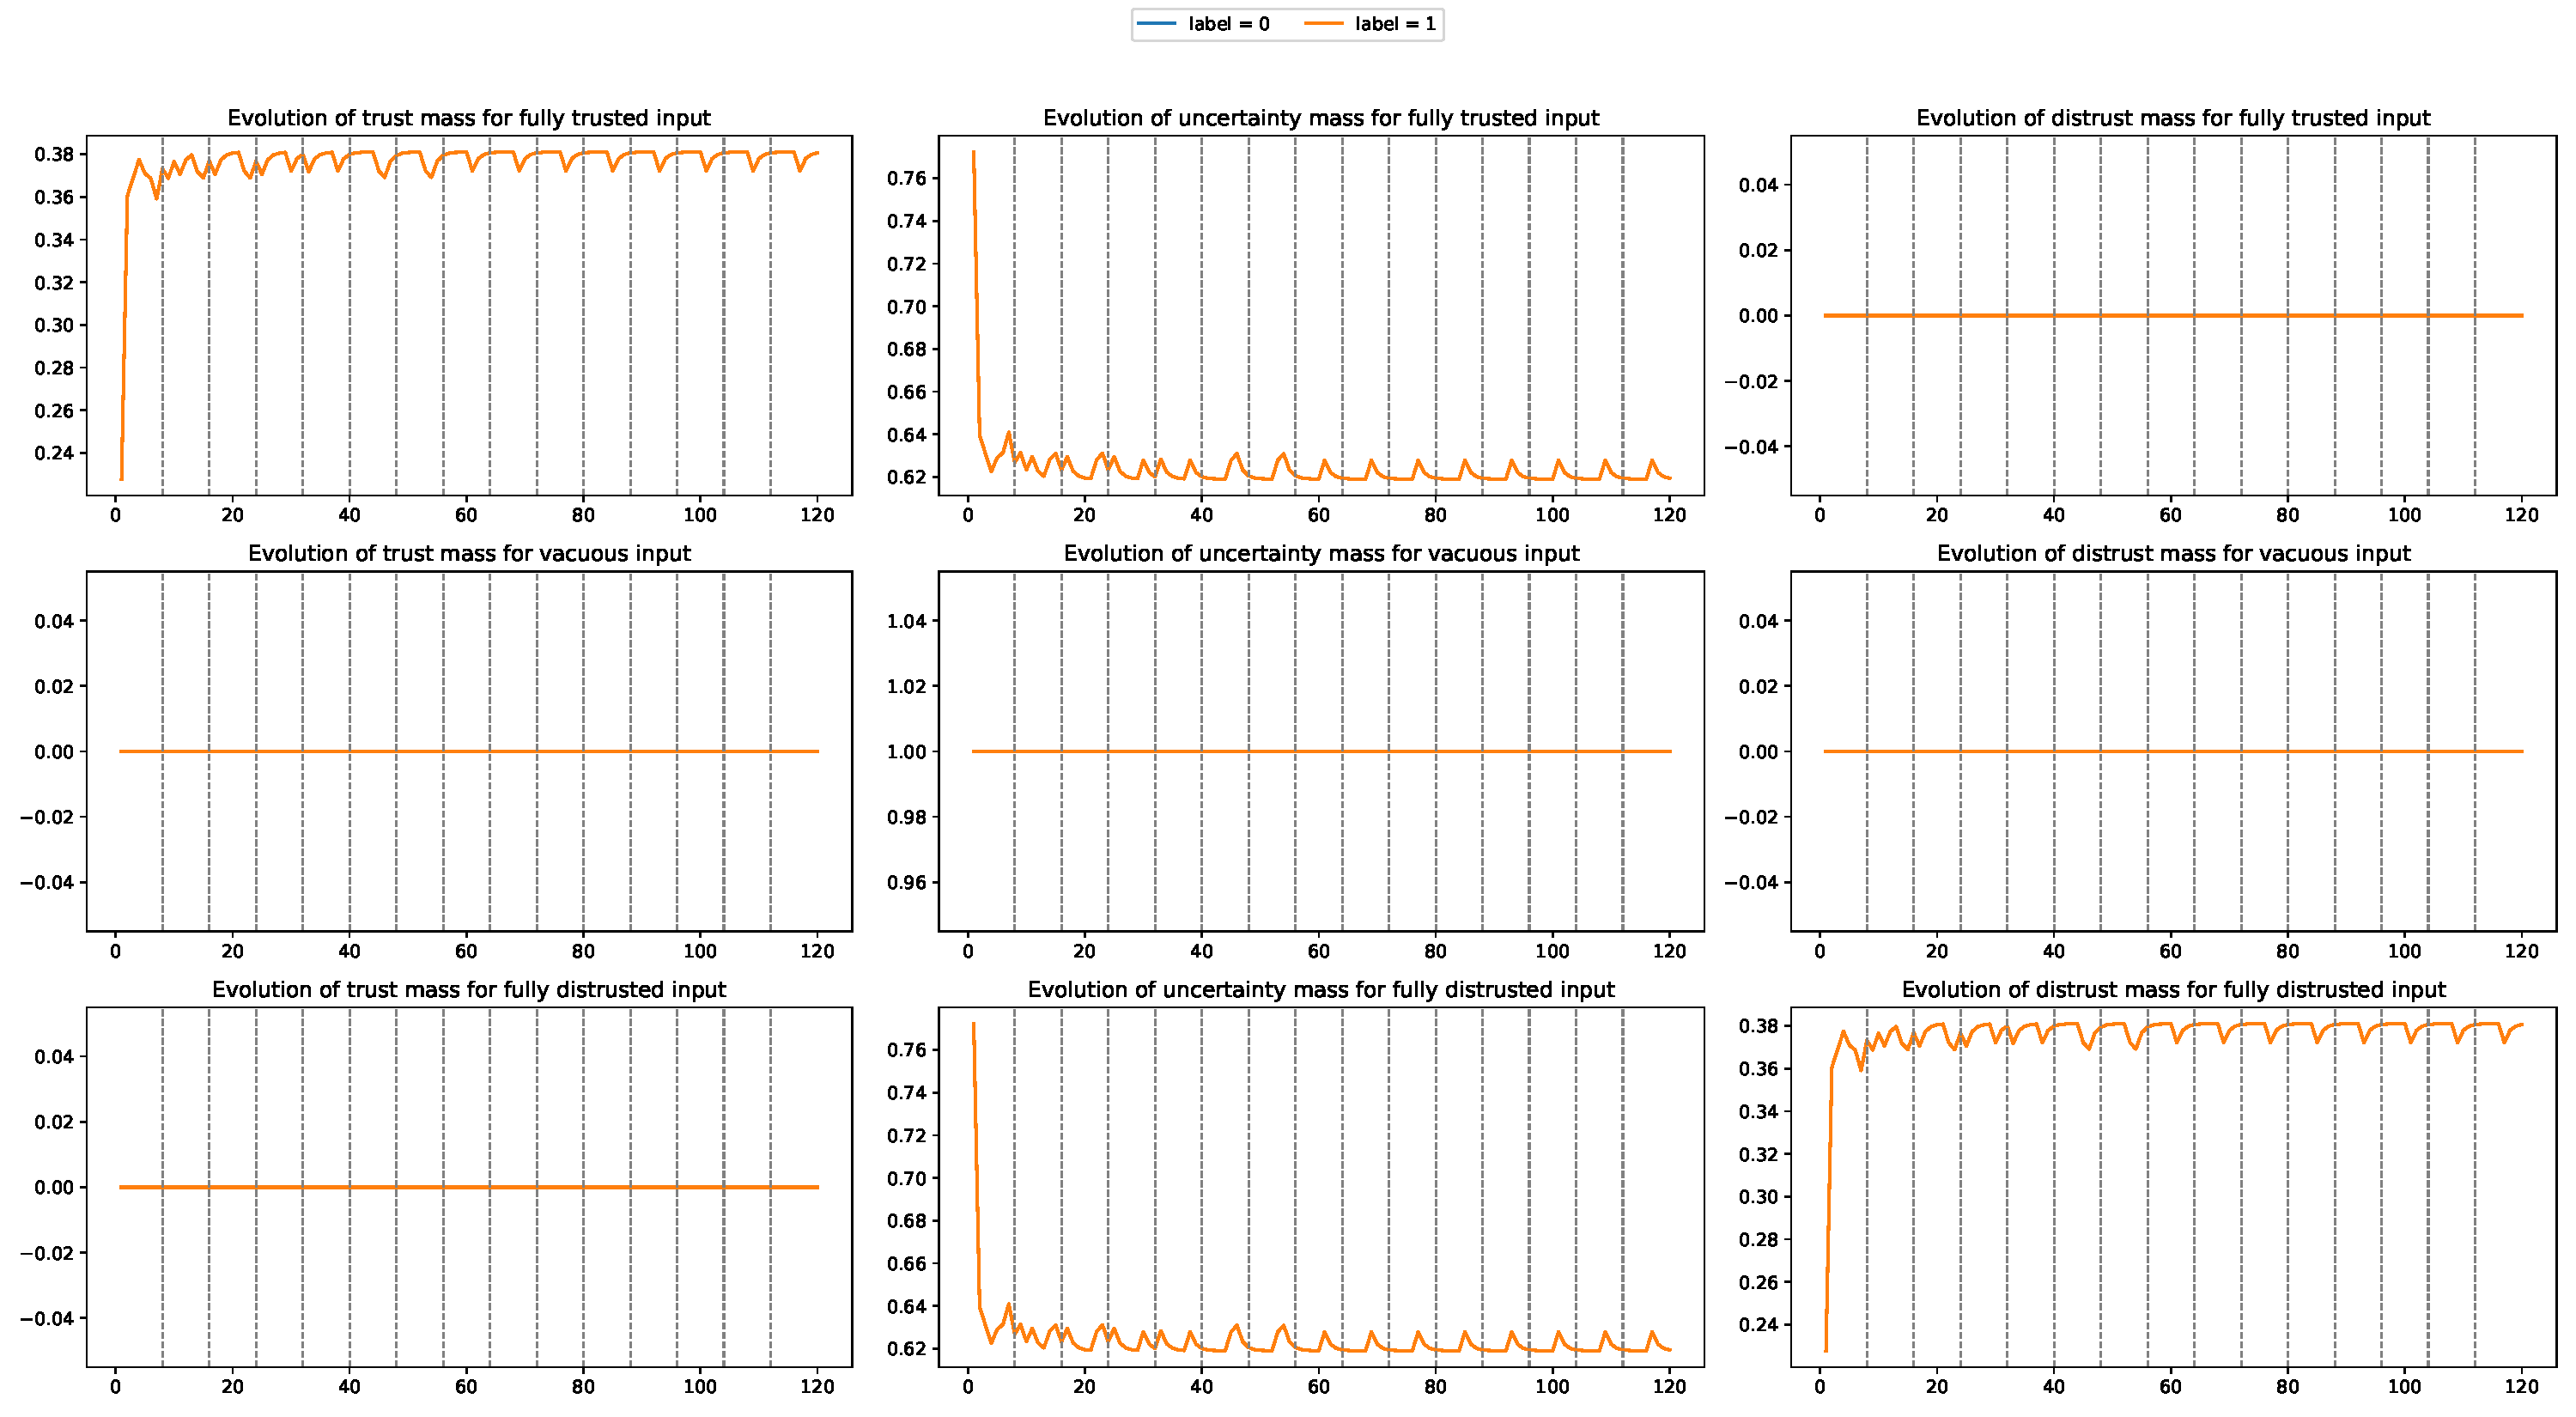
\includegraphics[width=0.8\textwidth]{latex/PTAS_Eval_cancer_16_0.25_0.0_0.75_0.25_0.0_0.75_eps_0.1_PathSize_None__plot_ptas.pdf}
\caption{cancer\_16\_0.25,0.0,0.75\_0.25,0.0,0.75, $\varepsilon$=0.1}
\end{figure}

\begin{figure}[htbp]
\centering
  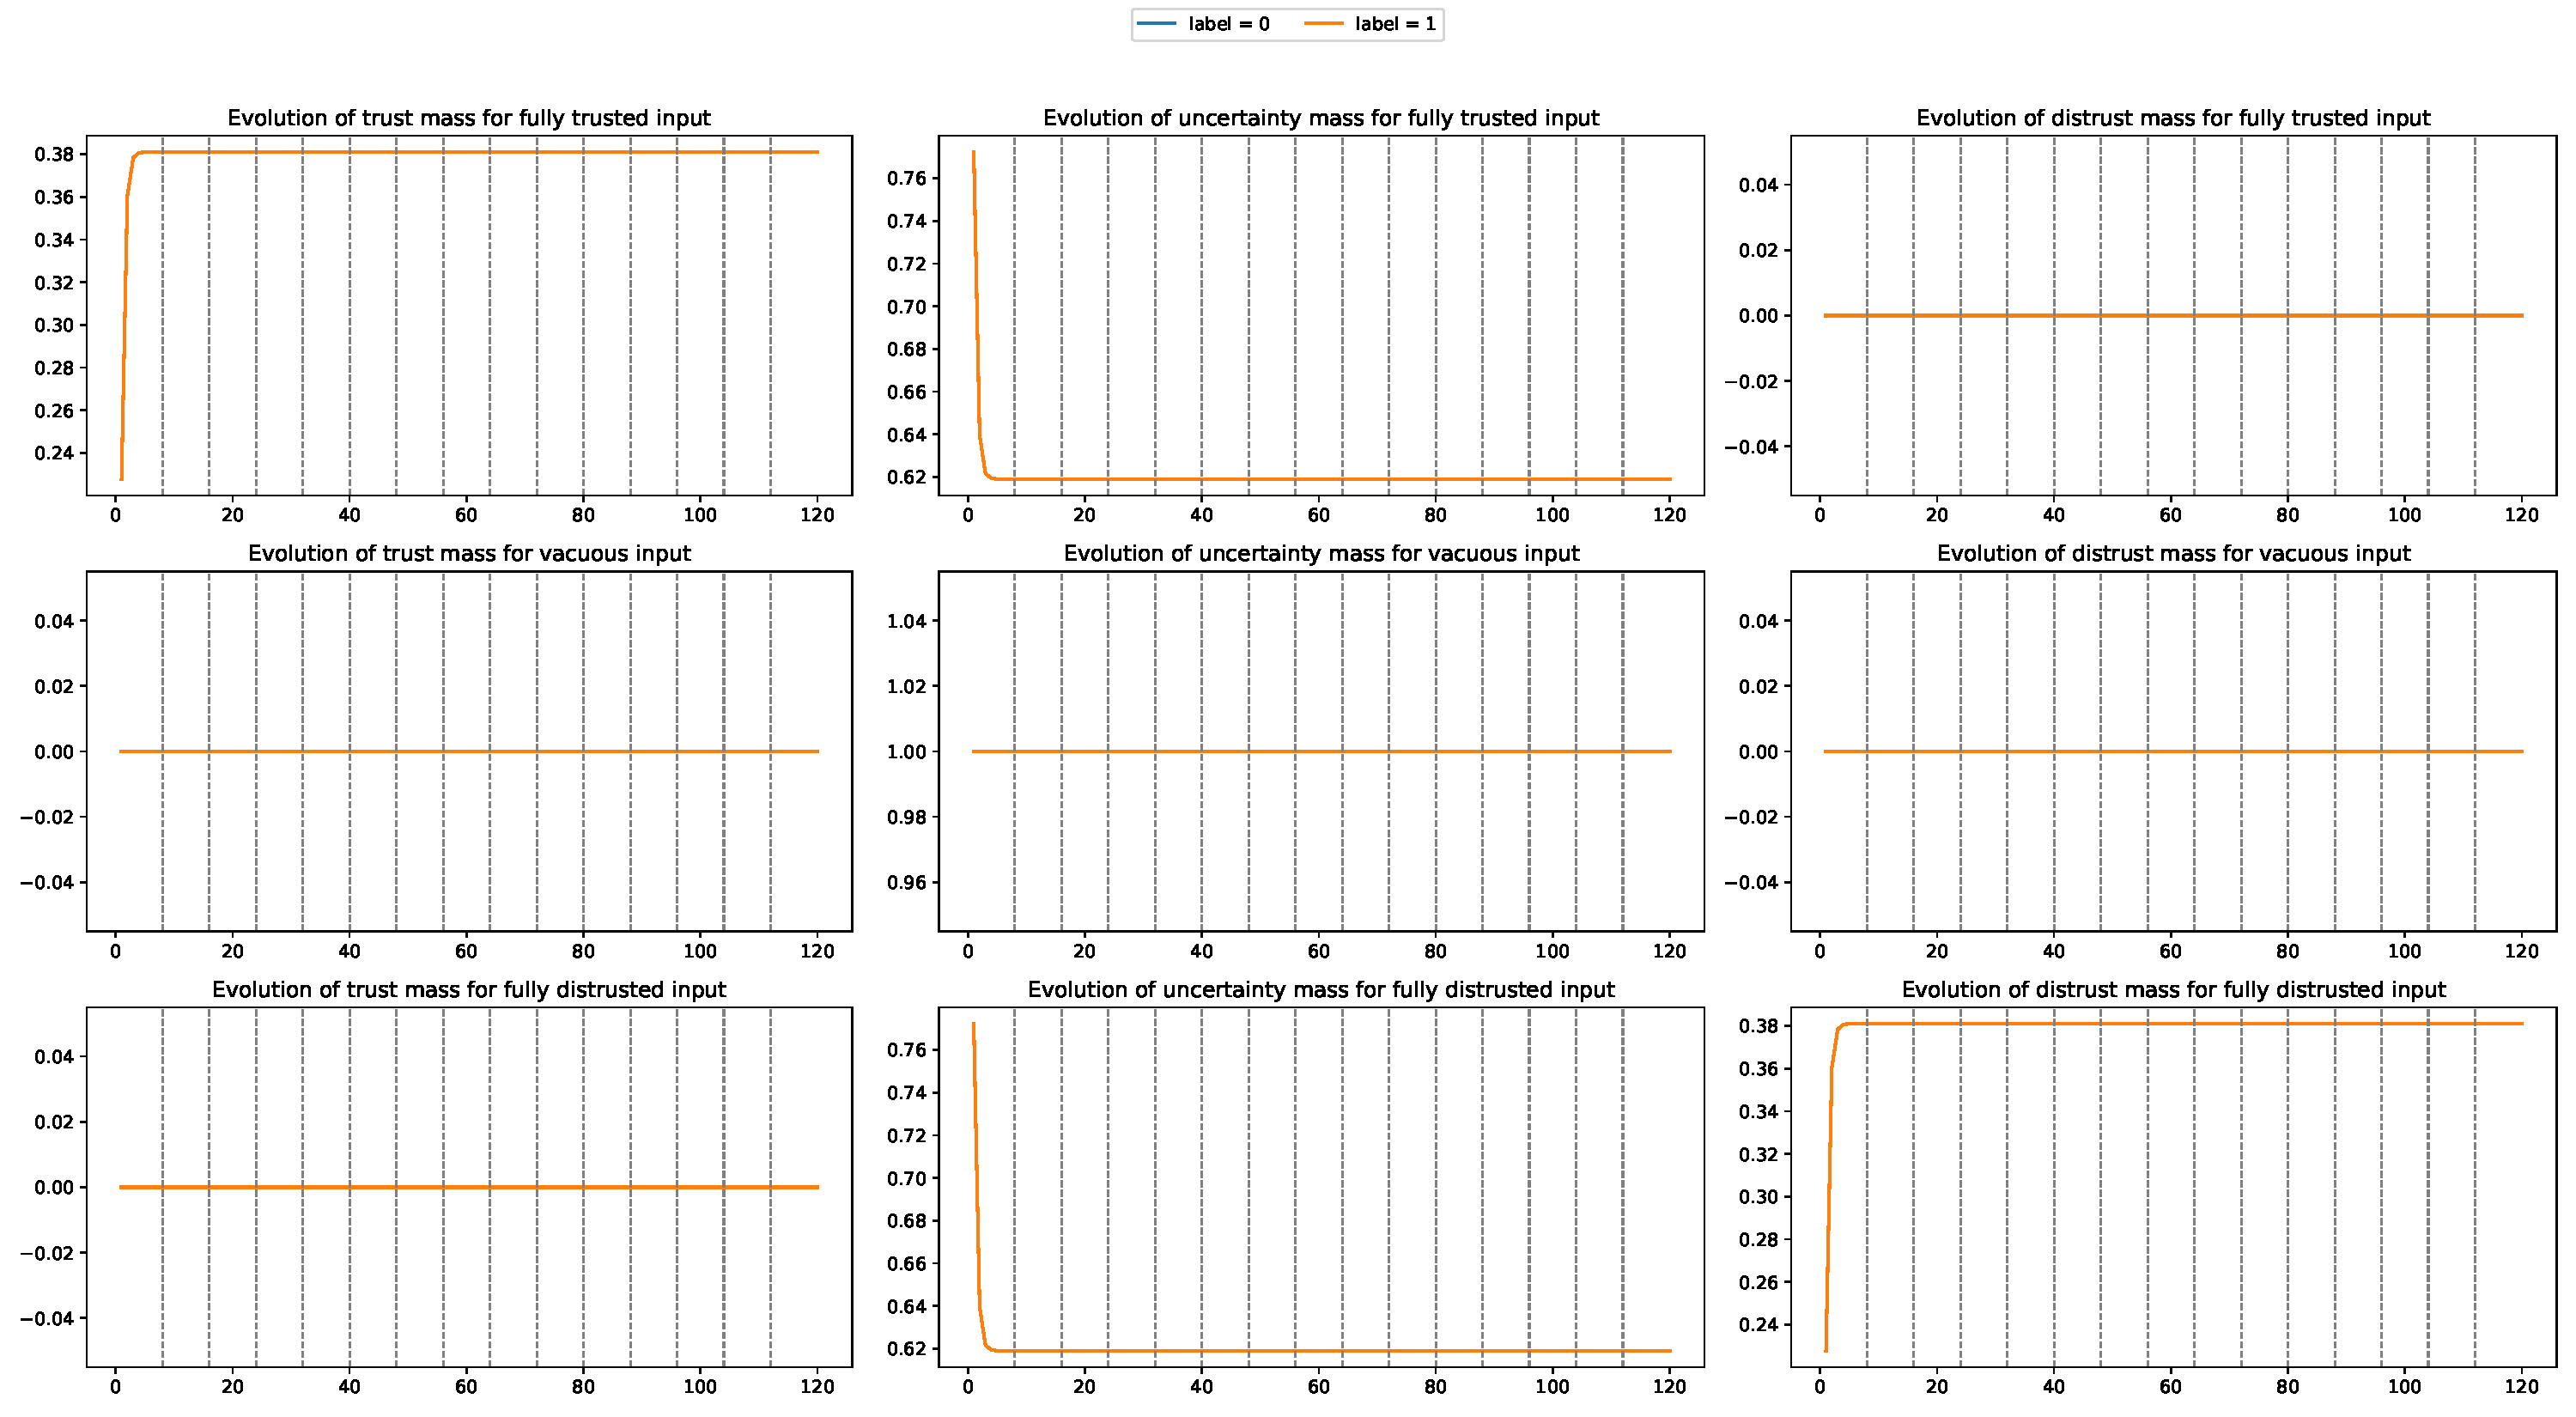
\includegraphics[width=0.8\textwidth]{latex/PTAS_Eval_cancer_16_0.25_0.0_0.75_0.25_0.0_0.75_eps_1_PathSize_None__plot_ptas.pdf}
\caption{cancer\_16\_0.25,0.0,0.75\_0.25,0.0,0.75, $\varepsilon$=1}
\end{figure}

\subsubsection{(0.25, 0.25, 0.5) -- (0.25, 0.25, 0.5)}

\begin{figure}[htbp]
\centering
  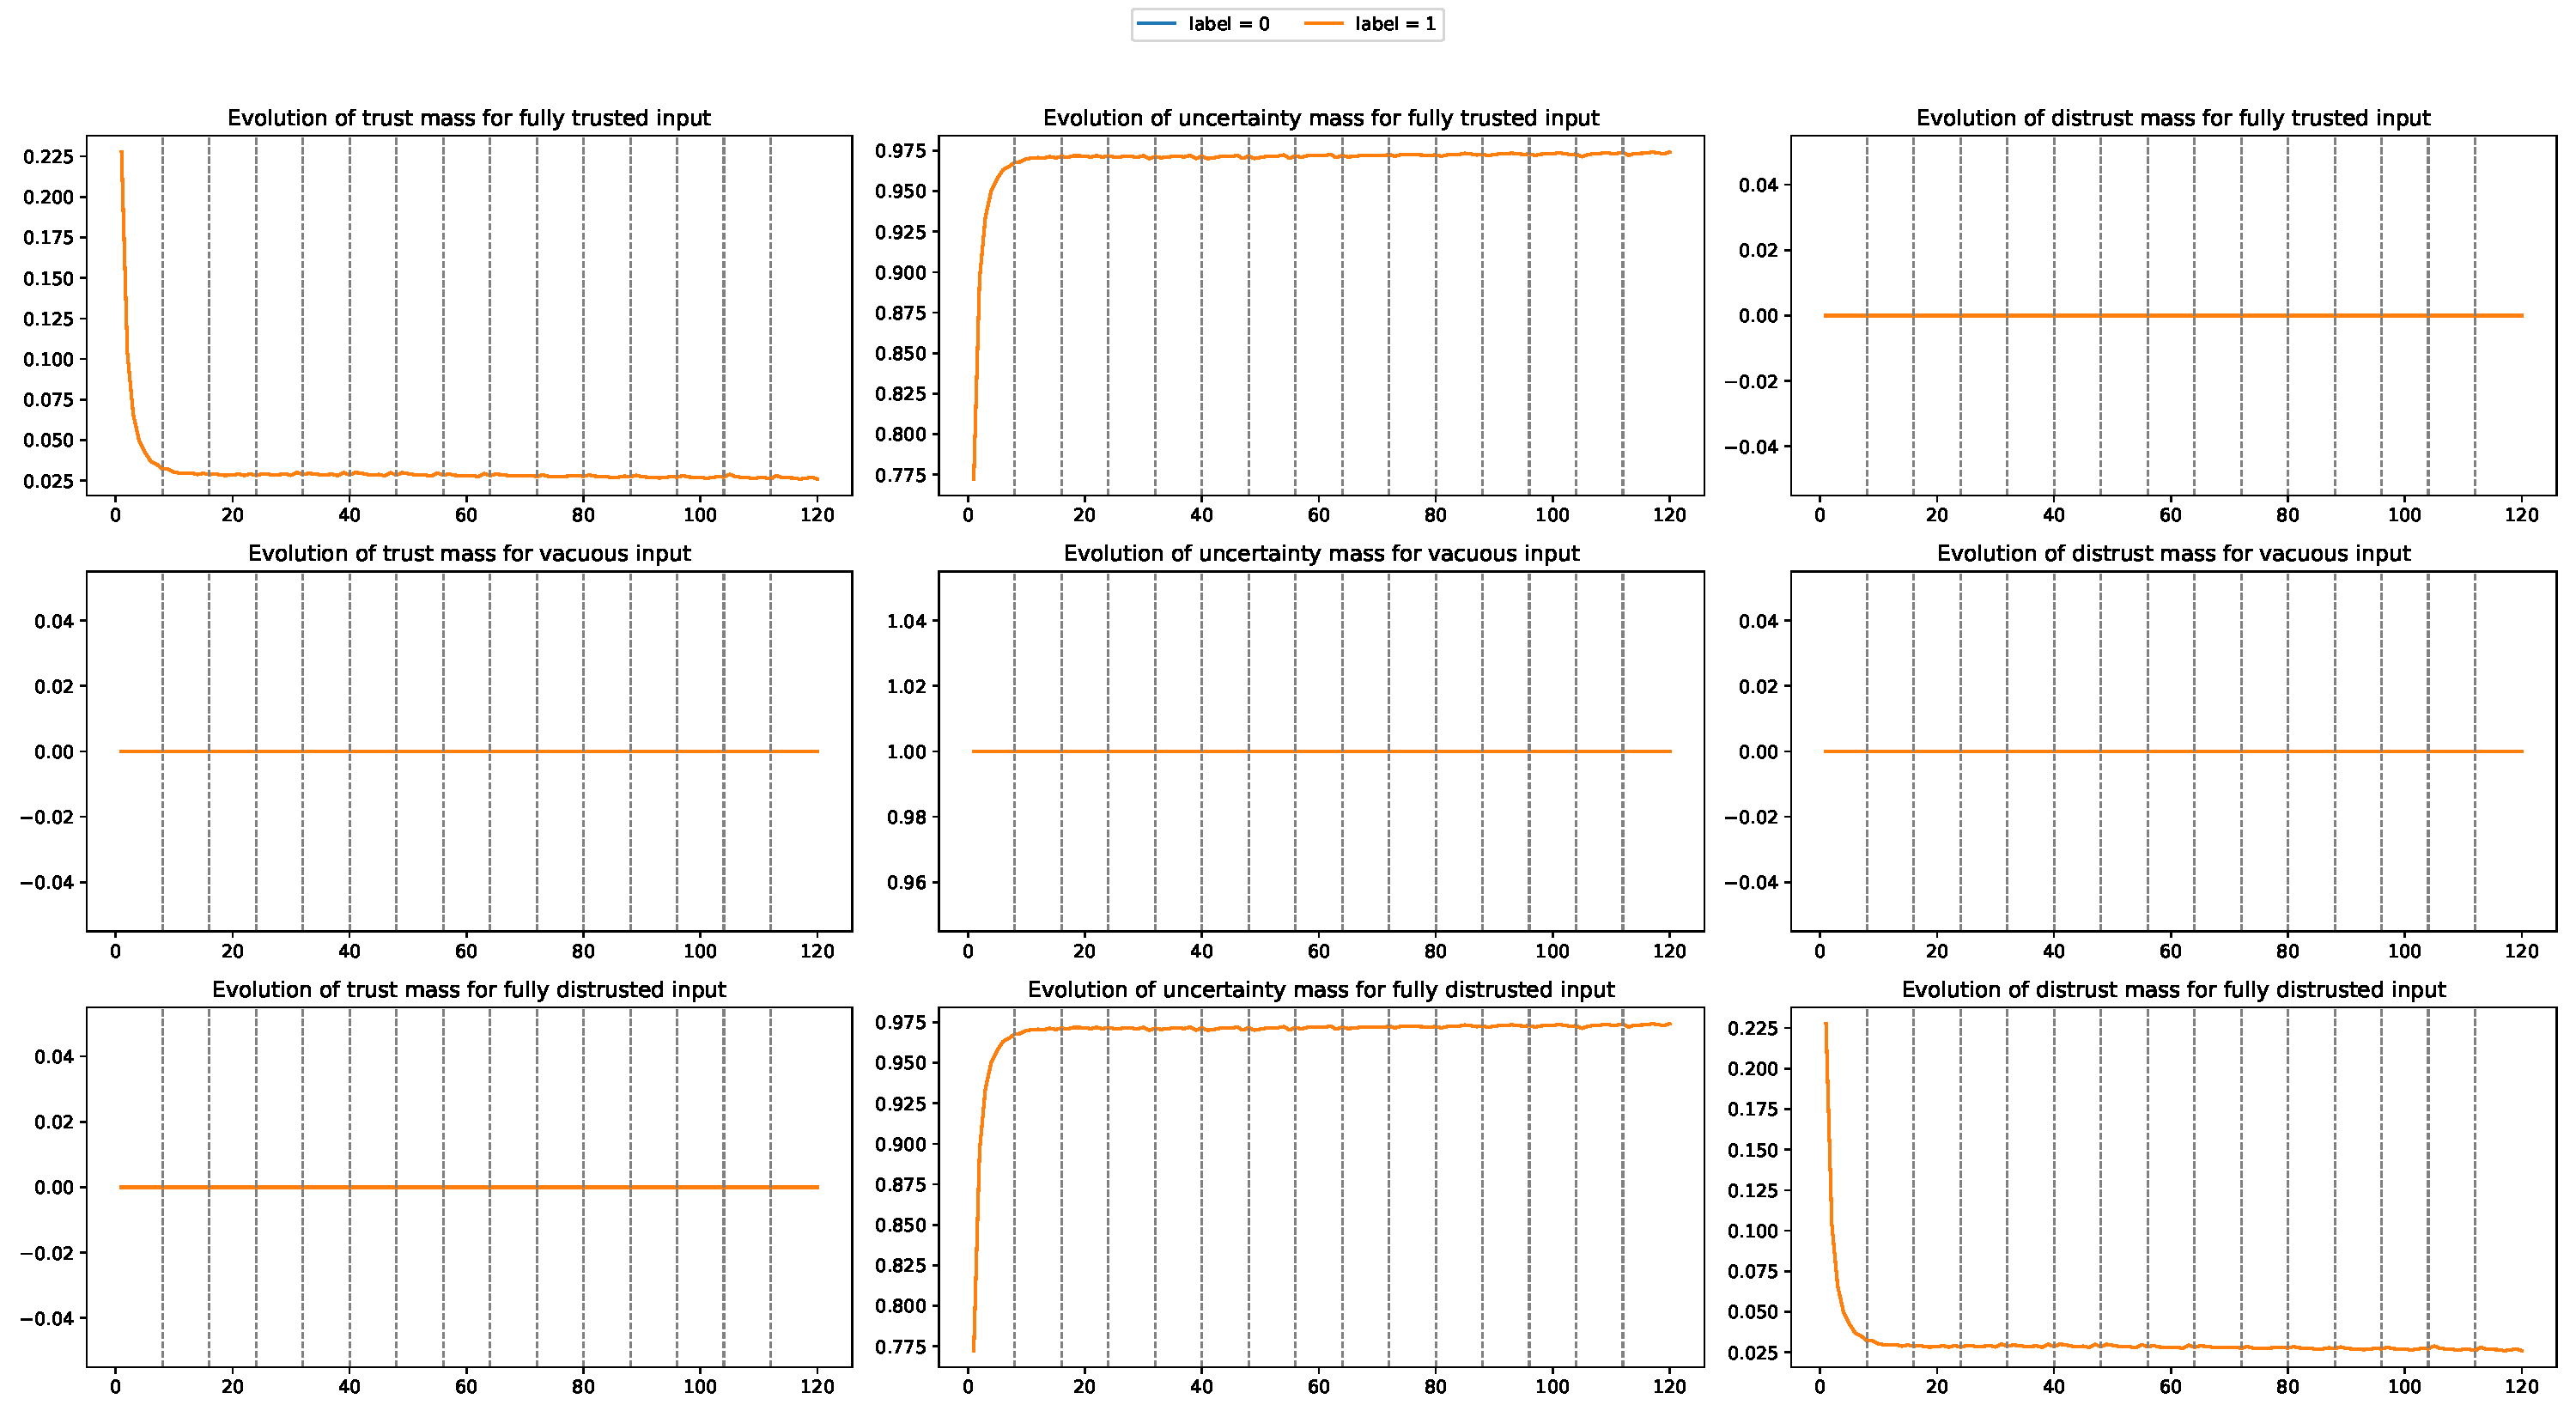
\includegraphics[width=0.8\textwidth]{latex/PTAS_Eval_cancer_16_0.25_0.25_0.5_0.25_0.25_0.5_eps_0.001_PathSize_None__plot_ptas.pdf}
\caption{cancer\_16\_0.25,0.25,0.5\_0.25,0.25,0.5, $\varepsilon$=0.001}
\end{figure}

\begin{figure}[htbp]
\centering
  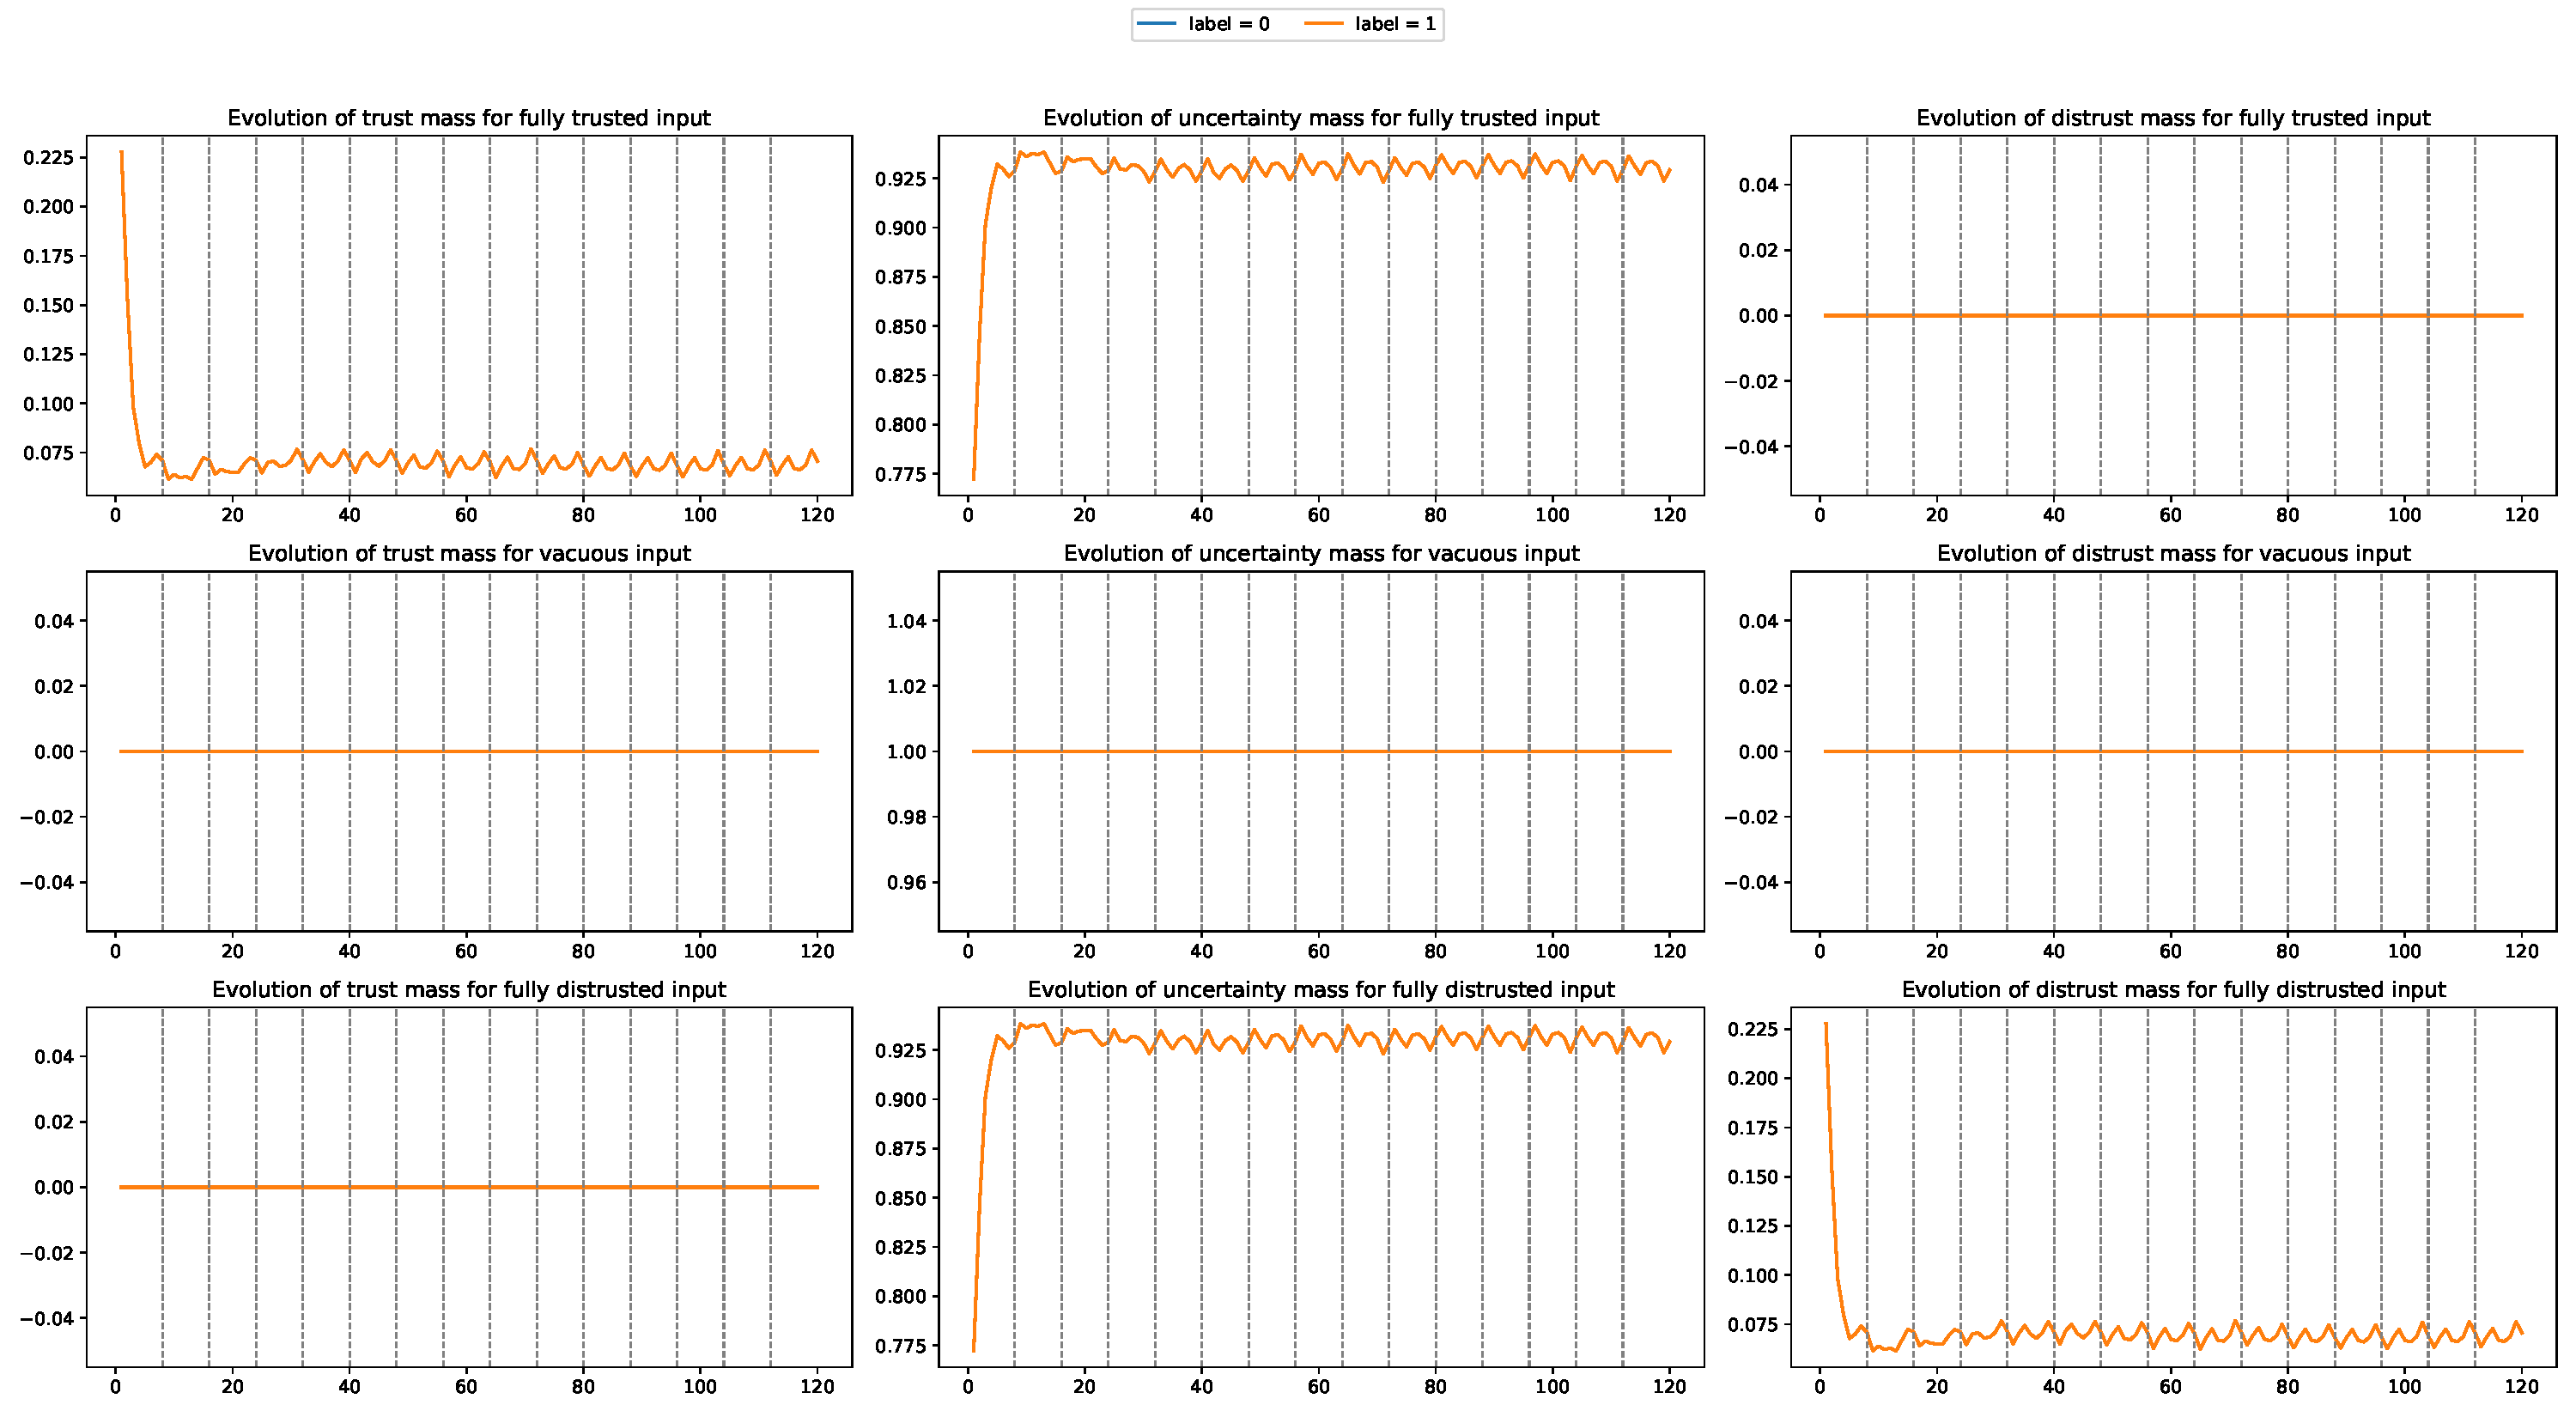
\includegraphics[width=0.8\textwidth]{latex/PTAS_Eval_cancer_16_0.25_0.25_0.5_0.25_0.25_0.5_eps_0.01_PathSize_None__plot_ptas.pdf}
\caption{cancer\_16\_0.25,0.25,0.5\_0.25,0.25,0.5, $\varepsilon$=0.01}
\end{figure}

\begin{figure}[htbp]
\centering
  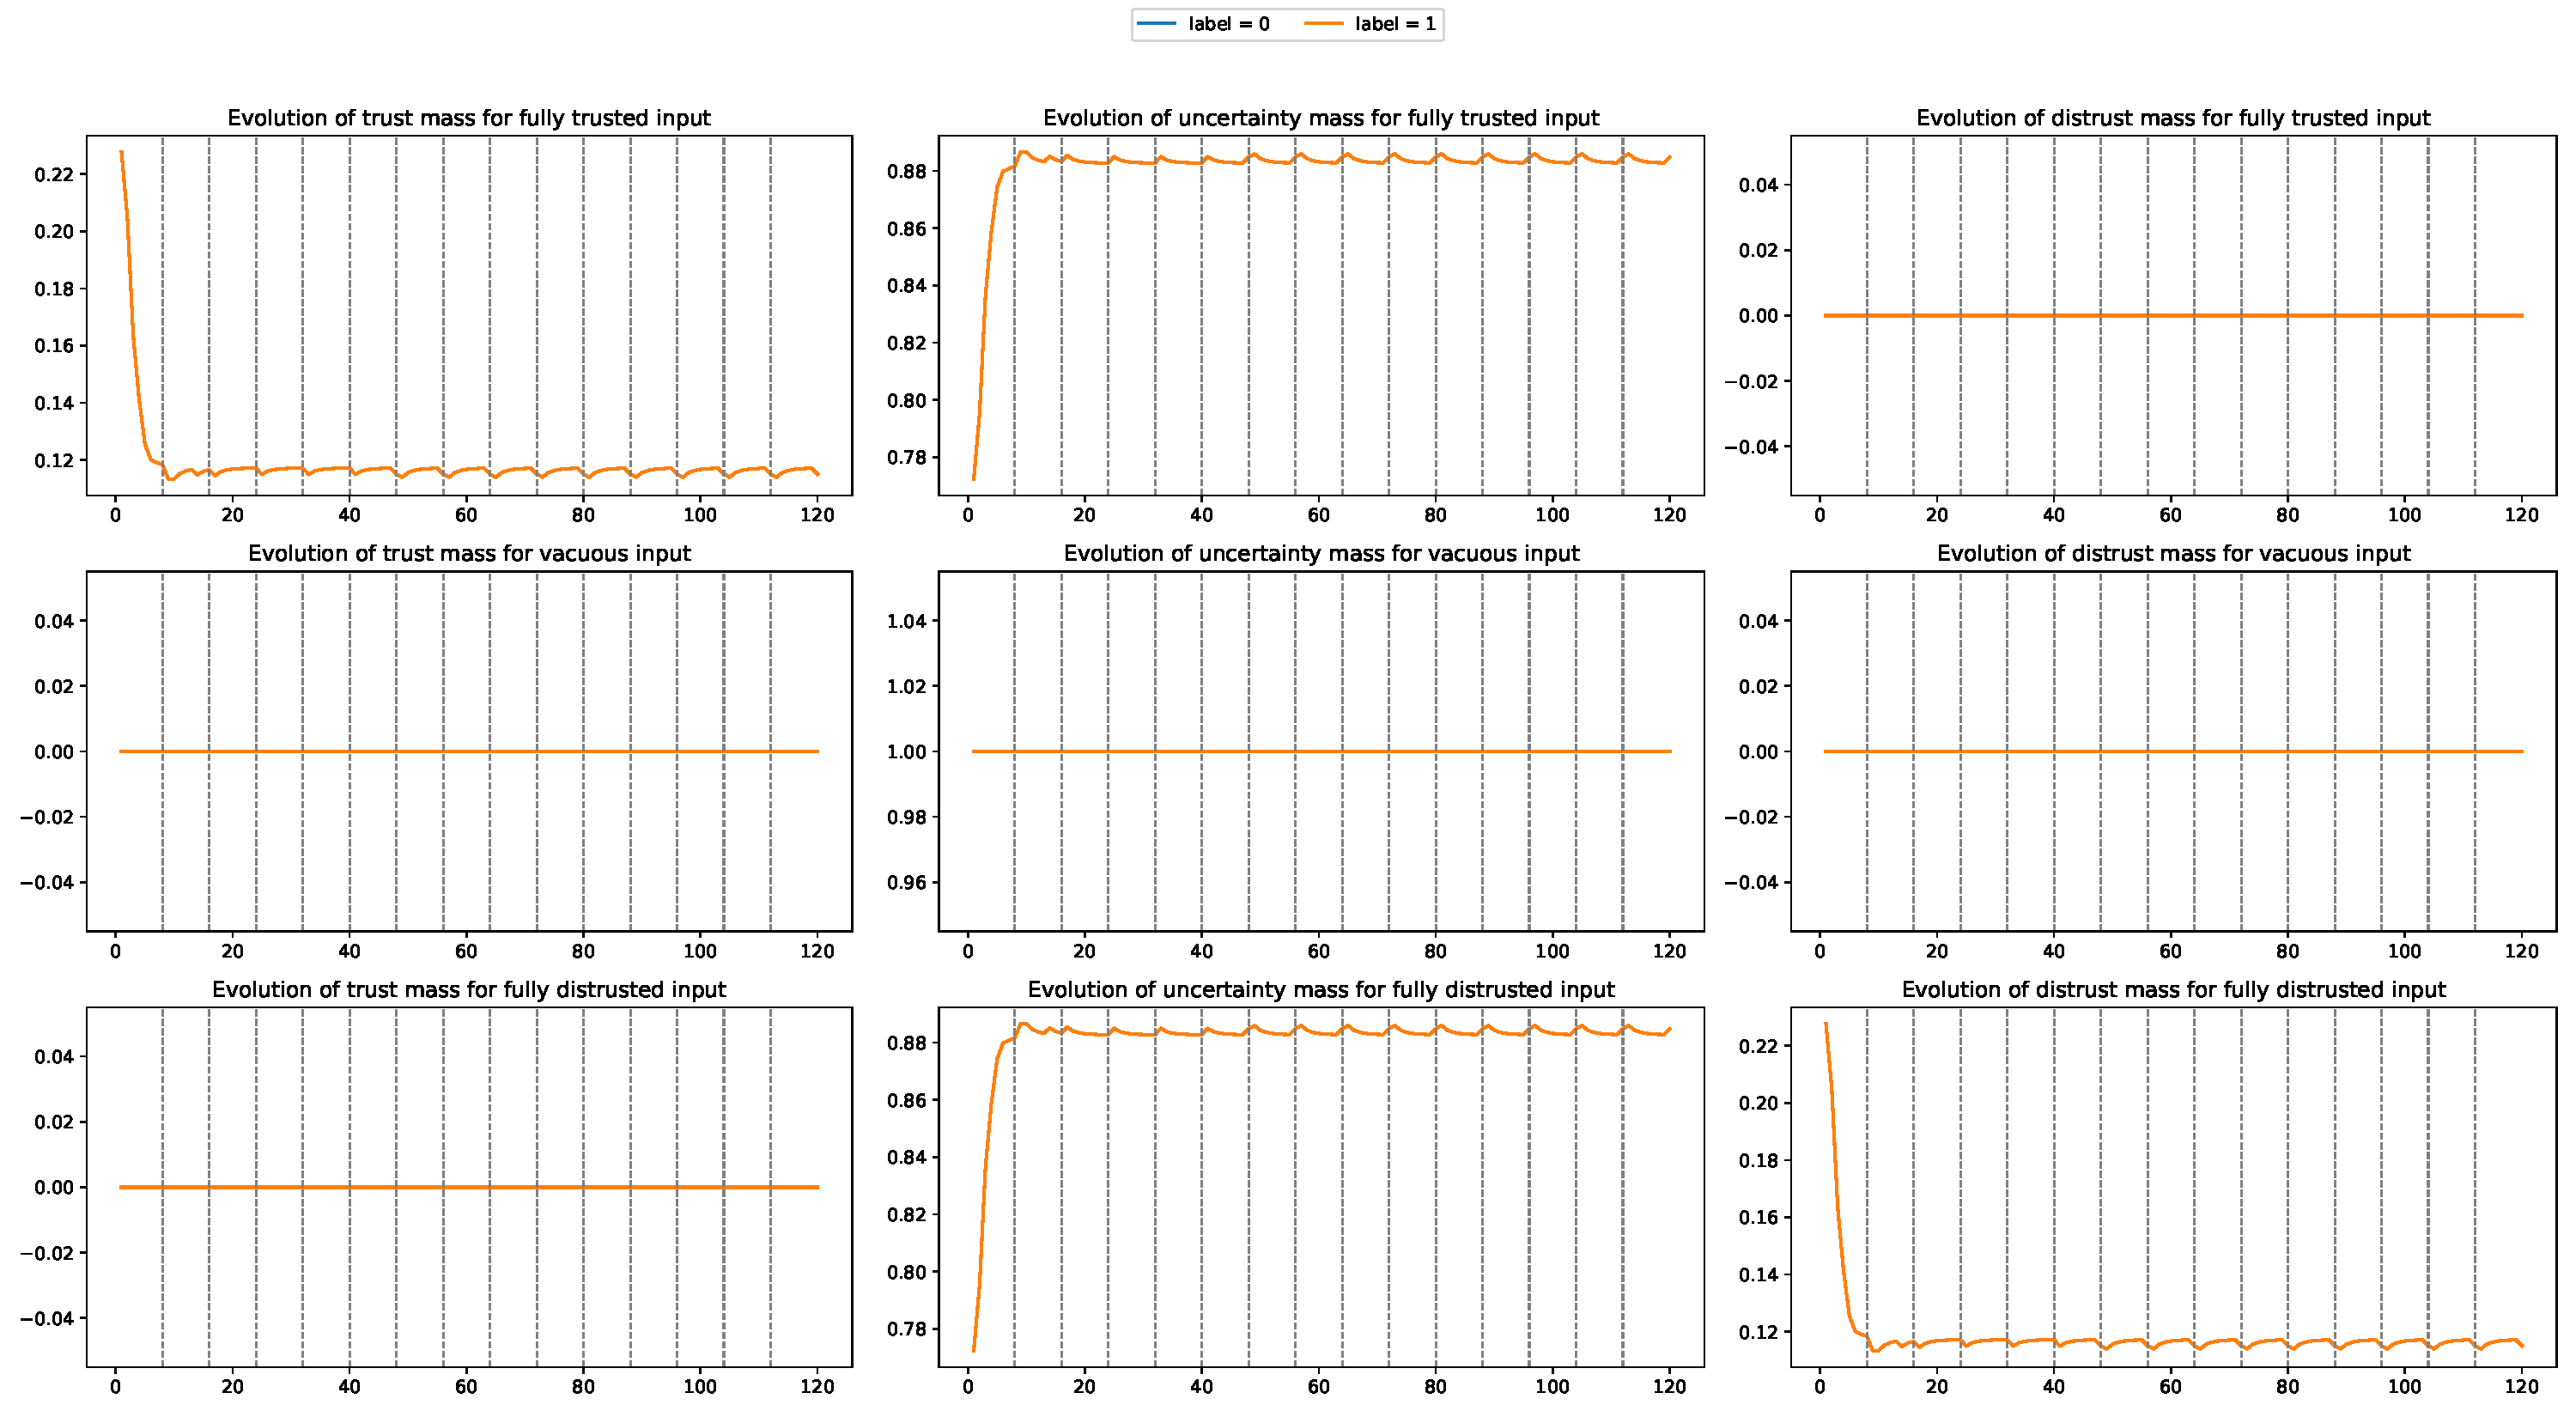
\includegraphics[width=0.8\textwidth]{latex/PTAS_Eval_cancer_16_0.25_0.25_0.5_0.25_0.25_0.5_eps_0.1_PathSize_None__plot_ptas.pdf}
\caption{cancer\_16\_0.25,0.25,0.5\_0.25,0.25,0.5, $\varepsilon$=0.1}
\end{figure}

\begin{figure}[htbp]
\centering
  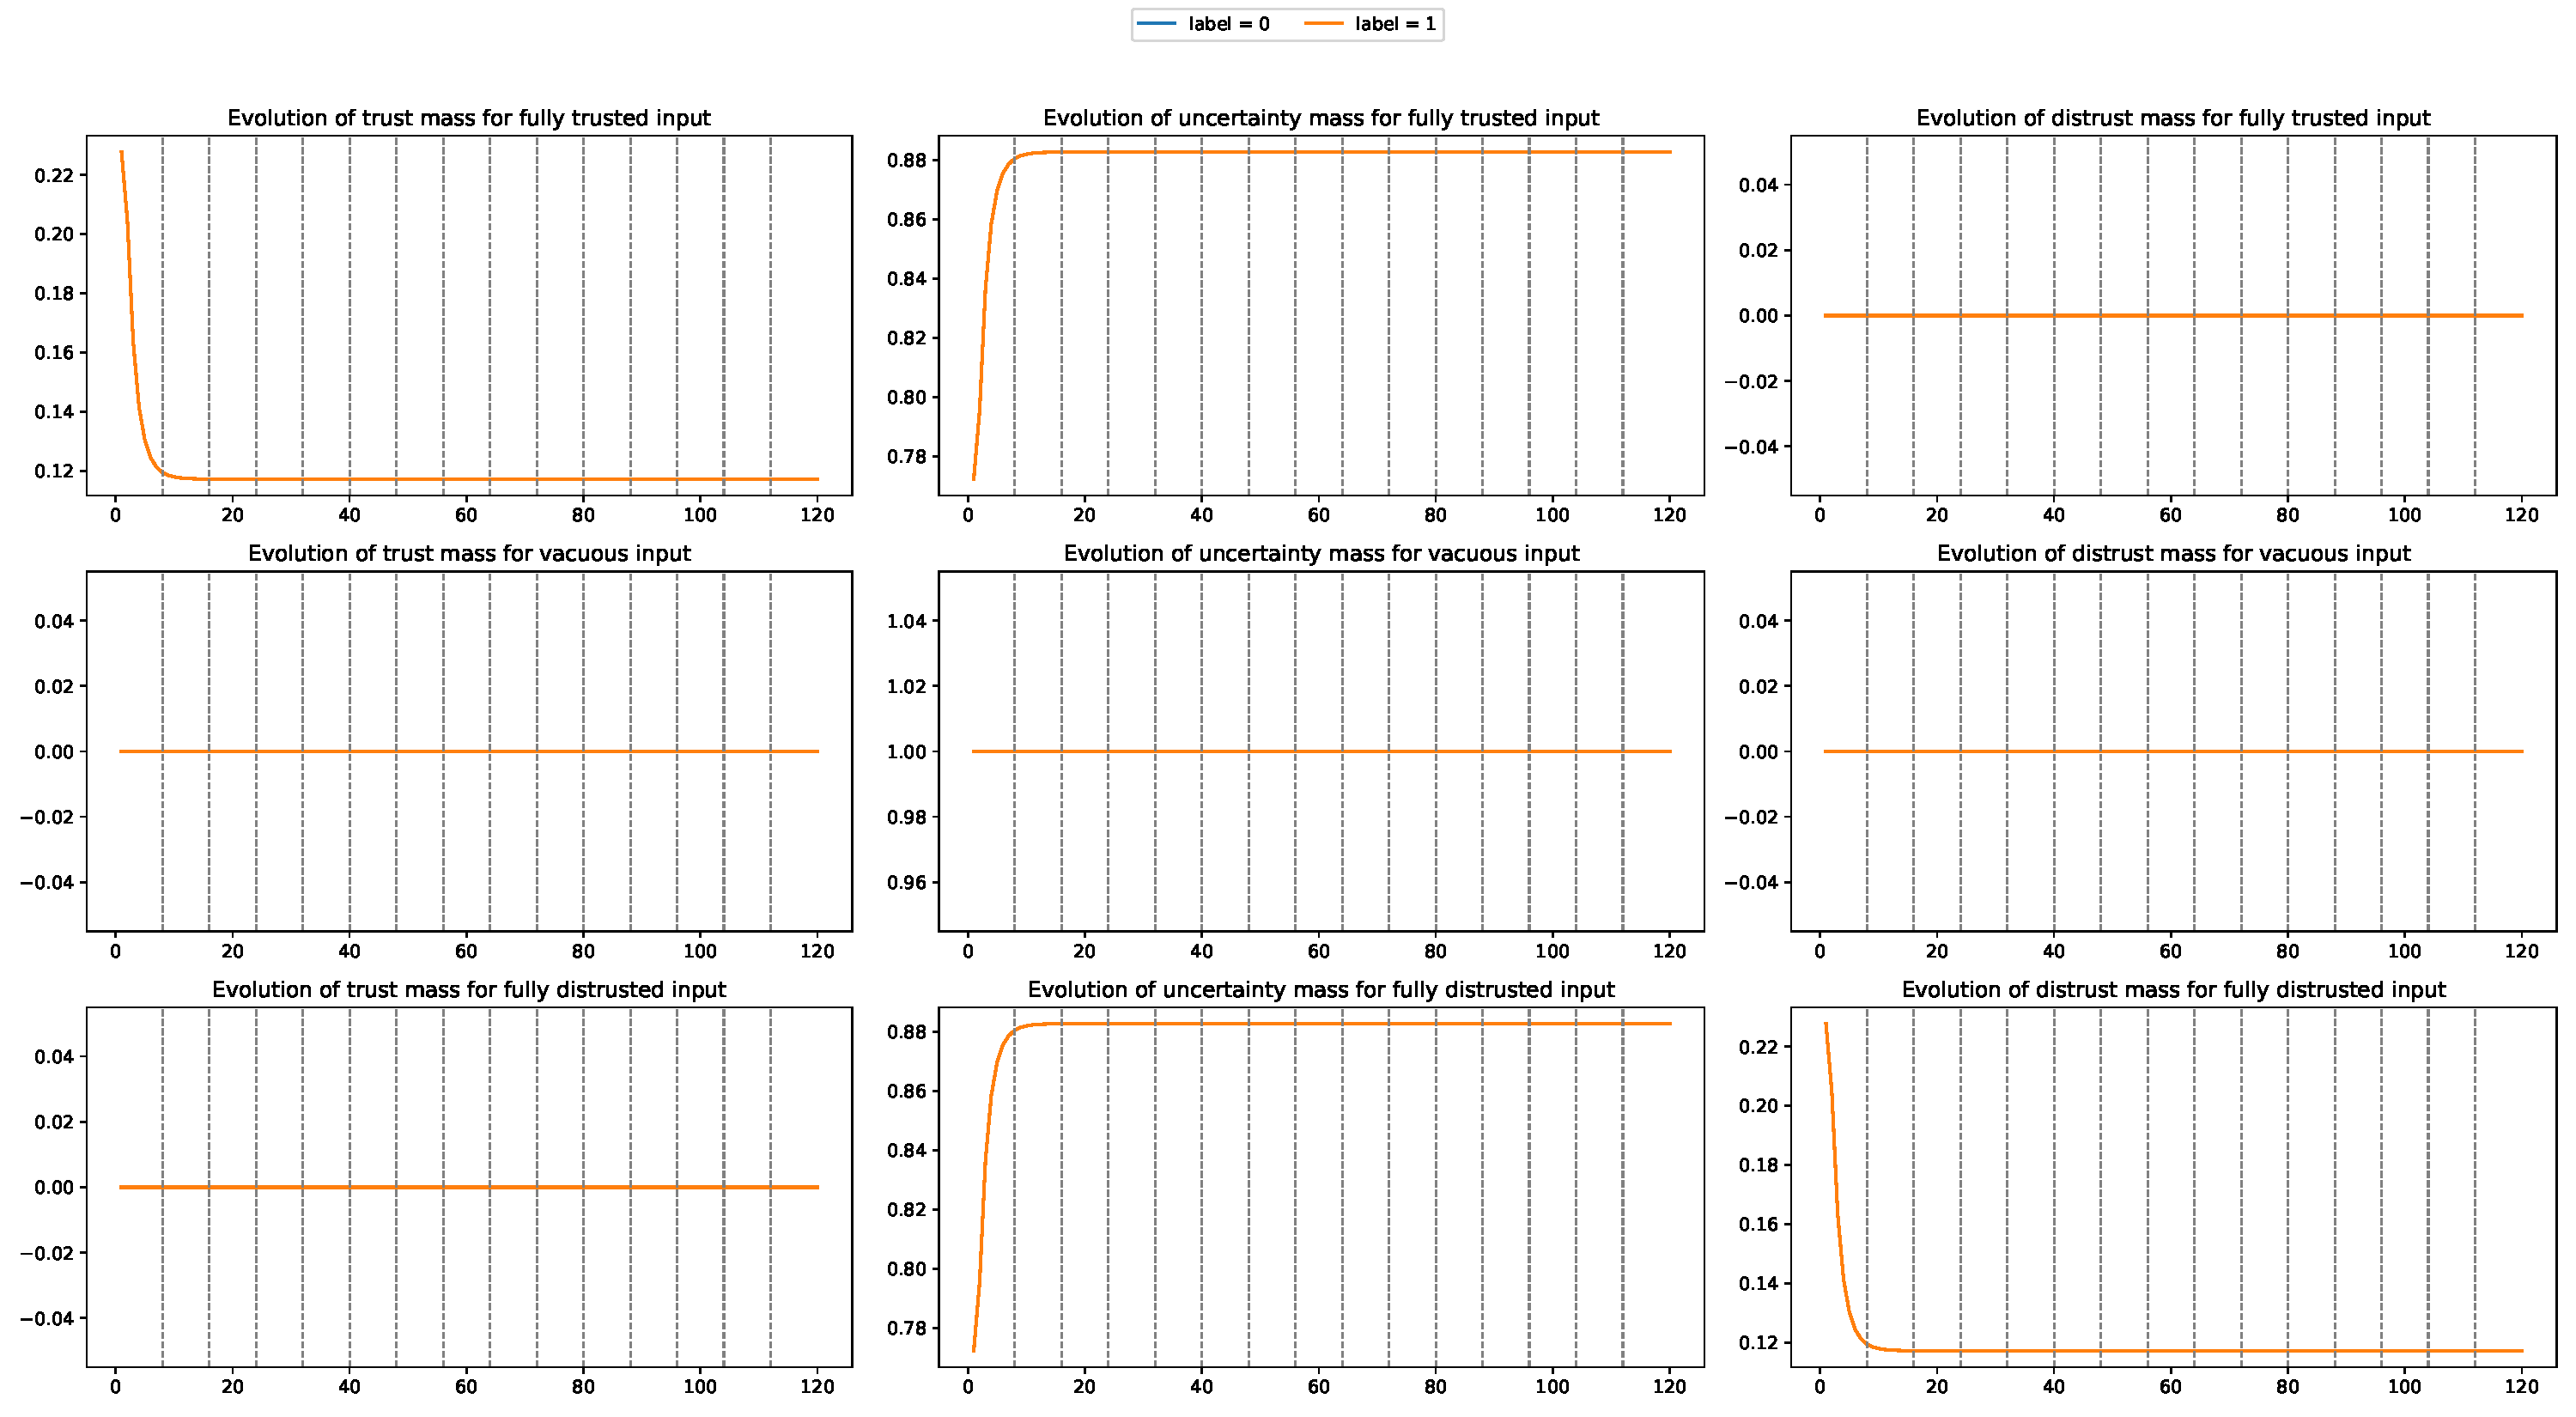
\includegraphics[width=0.8\textwidth]{latex/PTAS_Eval_cancer_16_0.25_0.25_0.5_0.25_0.25_0.5_eps_1_PathSize_None__plot_ptas.pdf}
\caption{cancer\_16\_0.25,0.25,0.5\_0.25,0.25,0.5, $\varepsilon$=1}
\end{figure}

\subsubsection{distrust -- distrust}

\begin{figure}[htbp]
\centering
  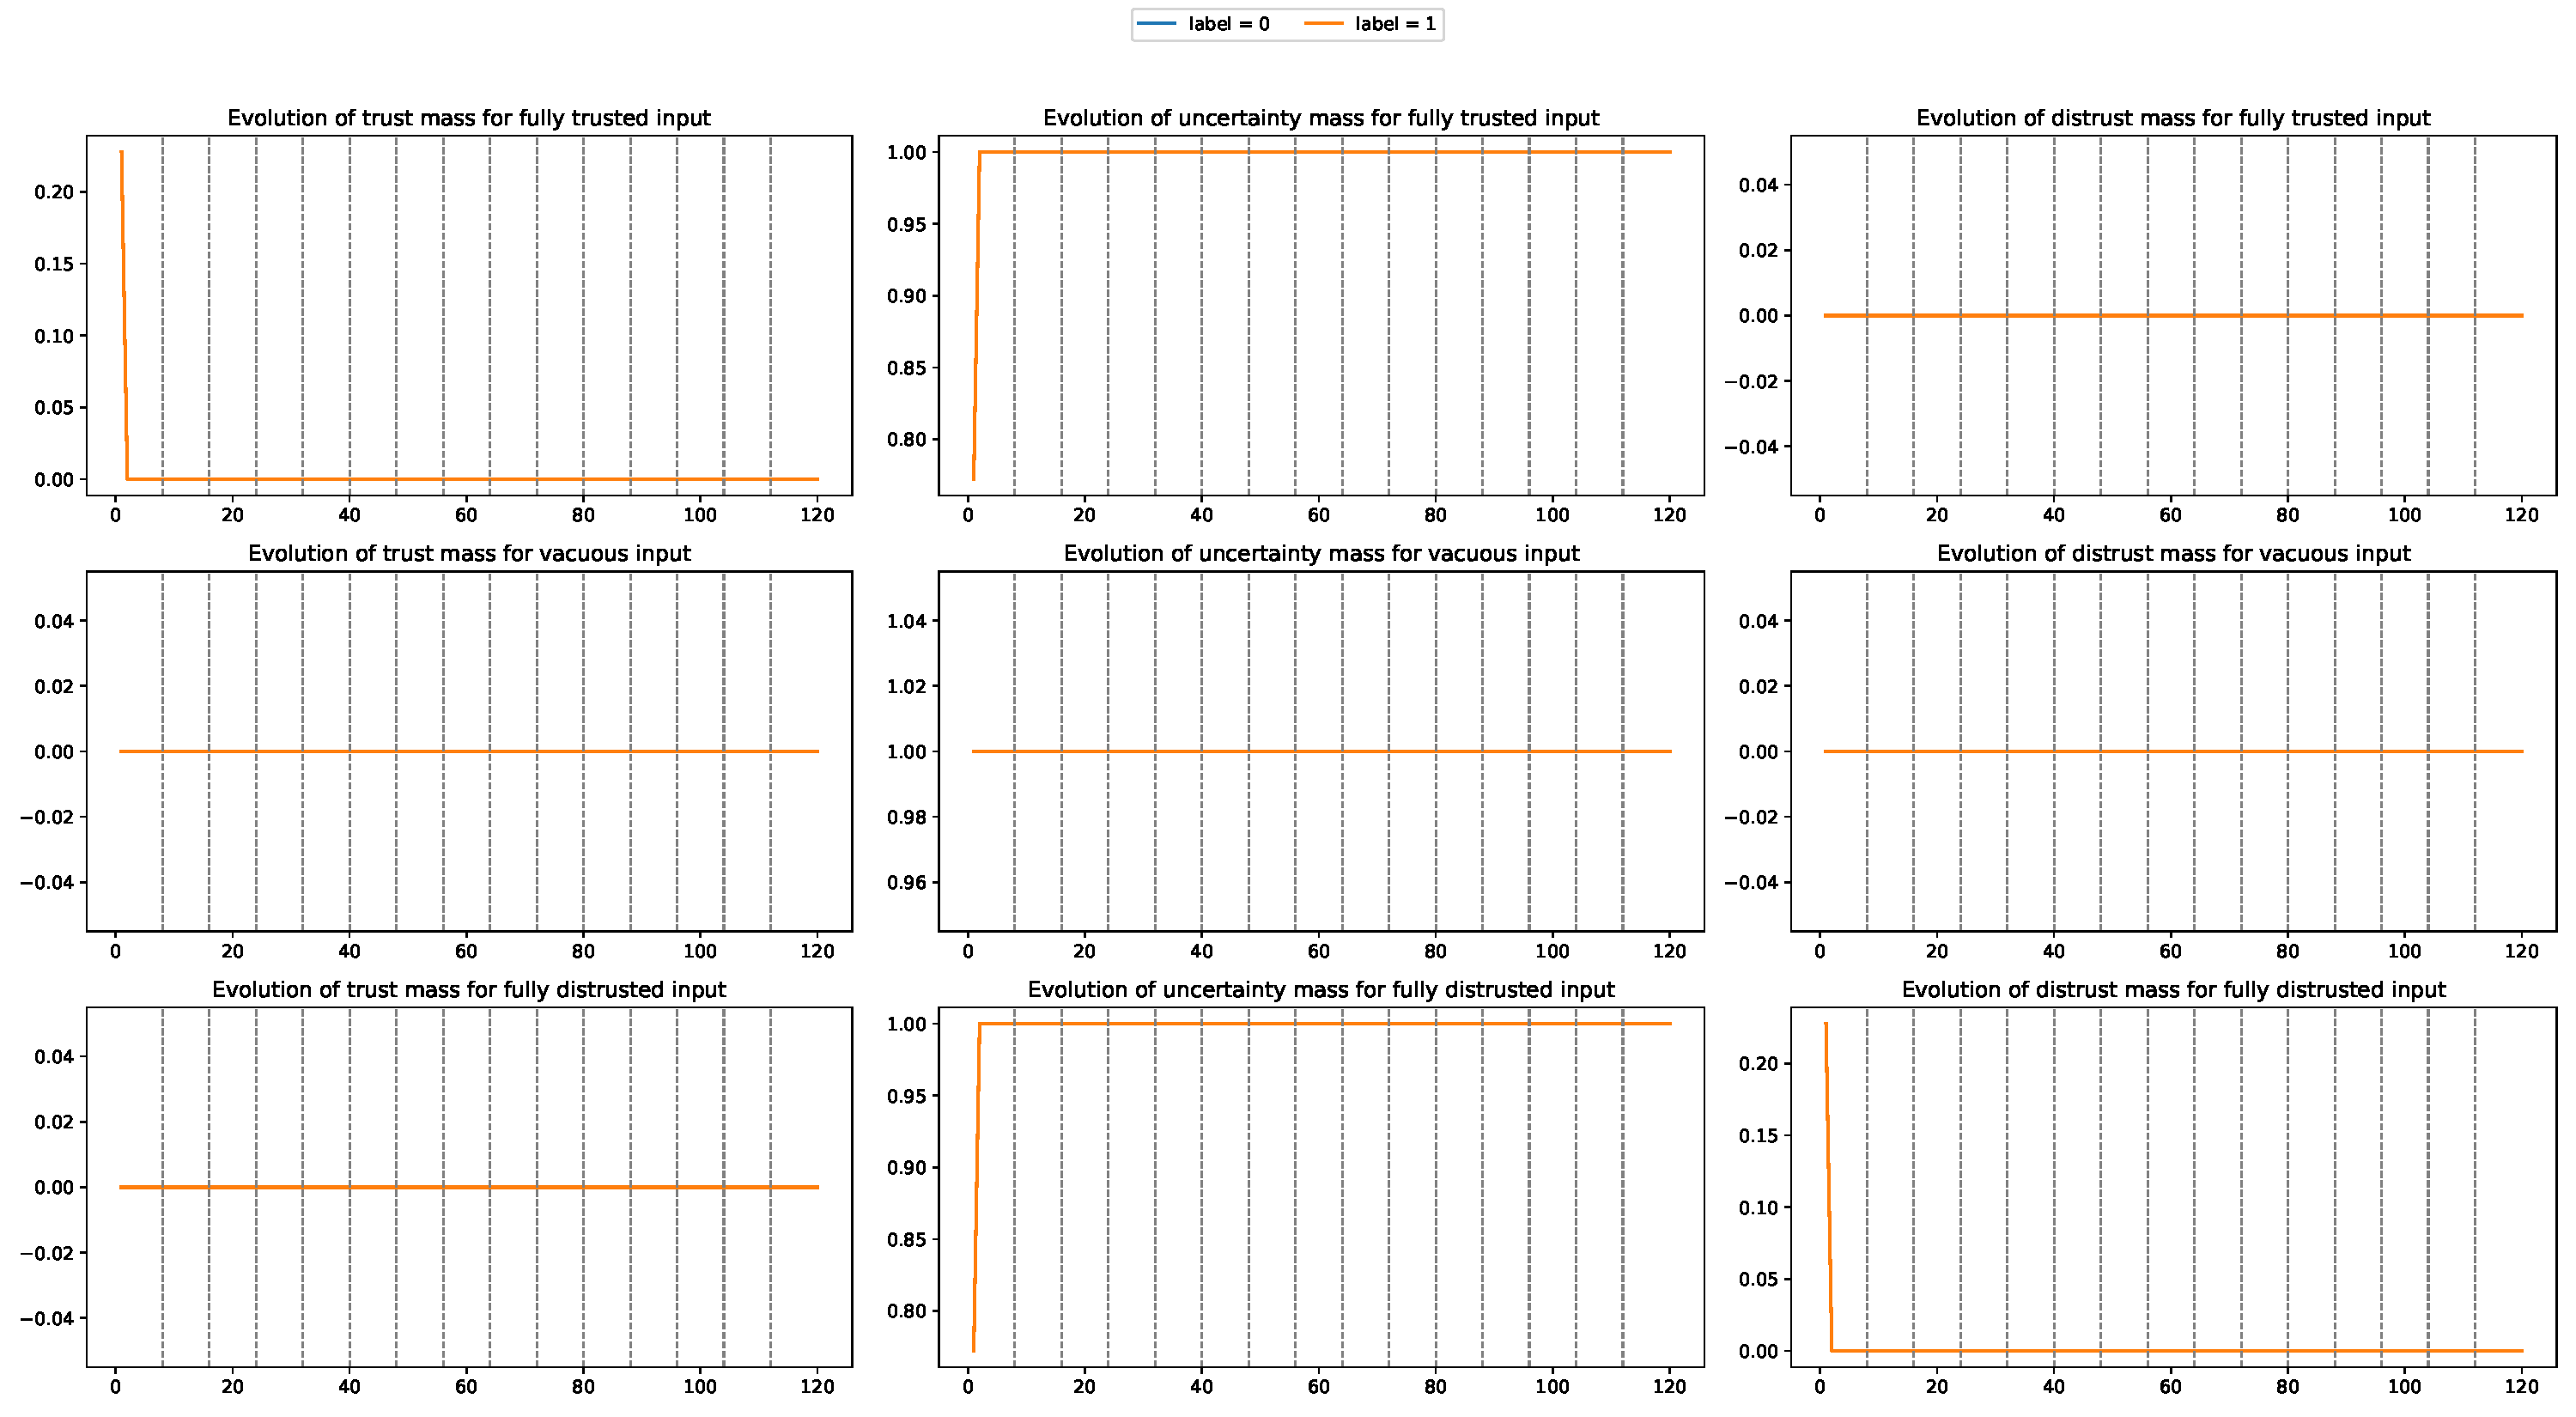
\includegraphics[width=0.8\textwidth]{latex/PTAS_Eval_cancer_16_distrust_distrust_eps_0.001_PathSize_None__plot_ptas.pdf}
\caption{cancer\_16\_distrust\_distrust, $\varepsilon$=0.001}
\end{figure}

\begin{figure}[htbp]
\centering
  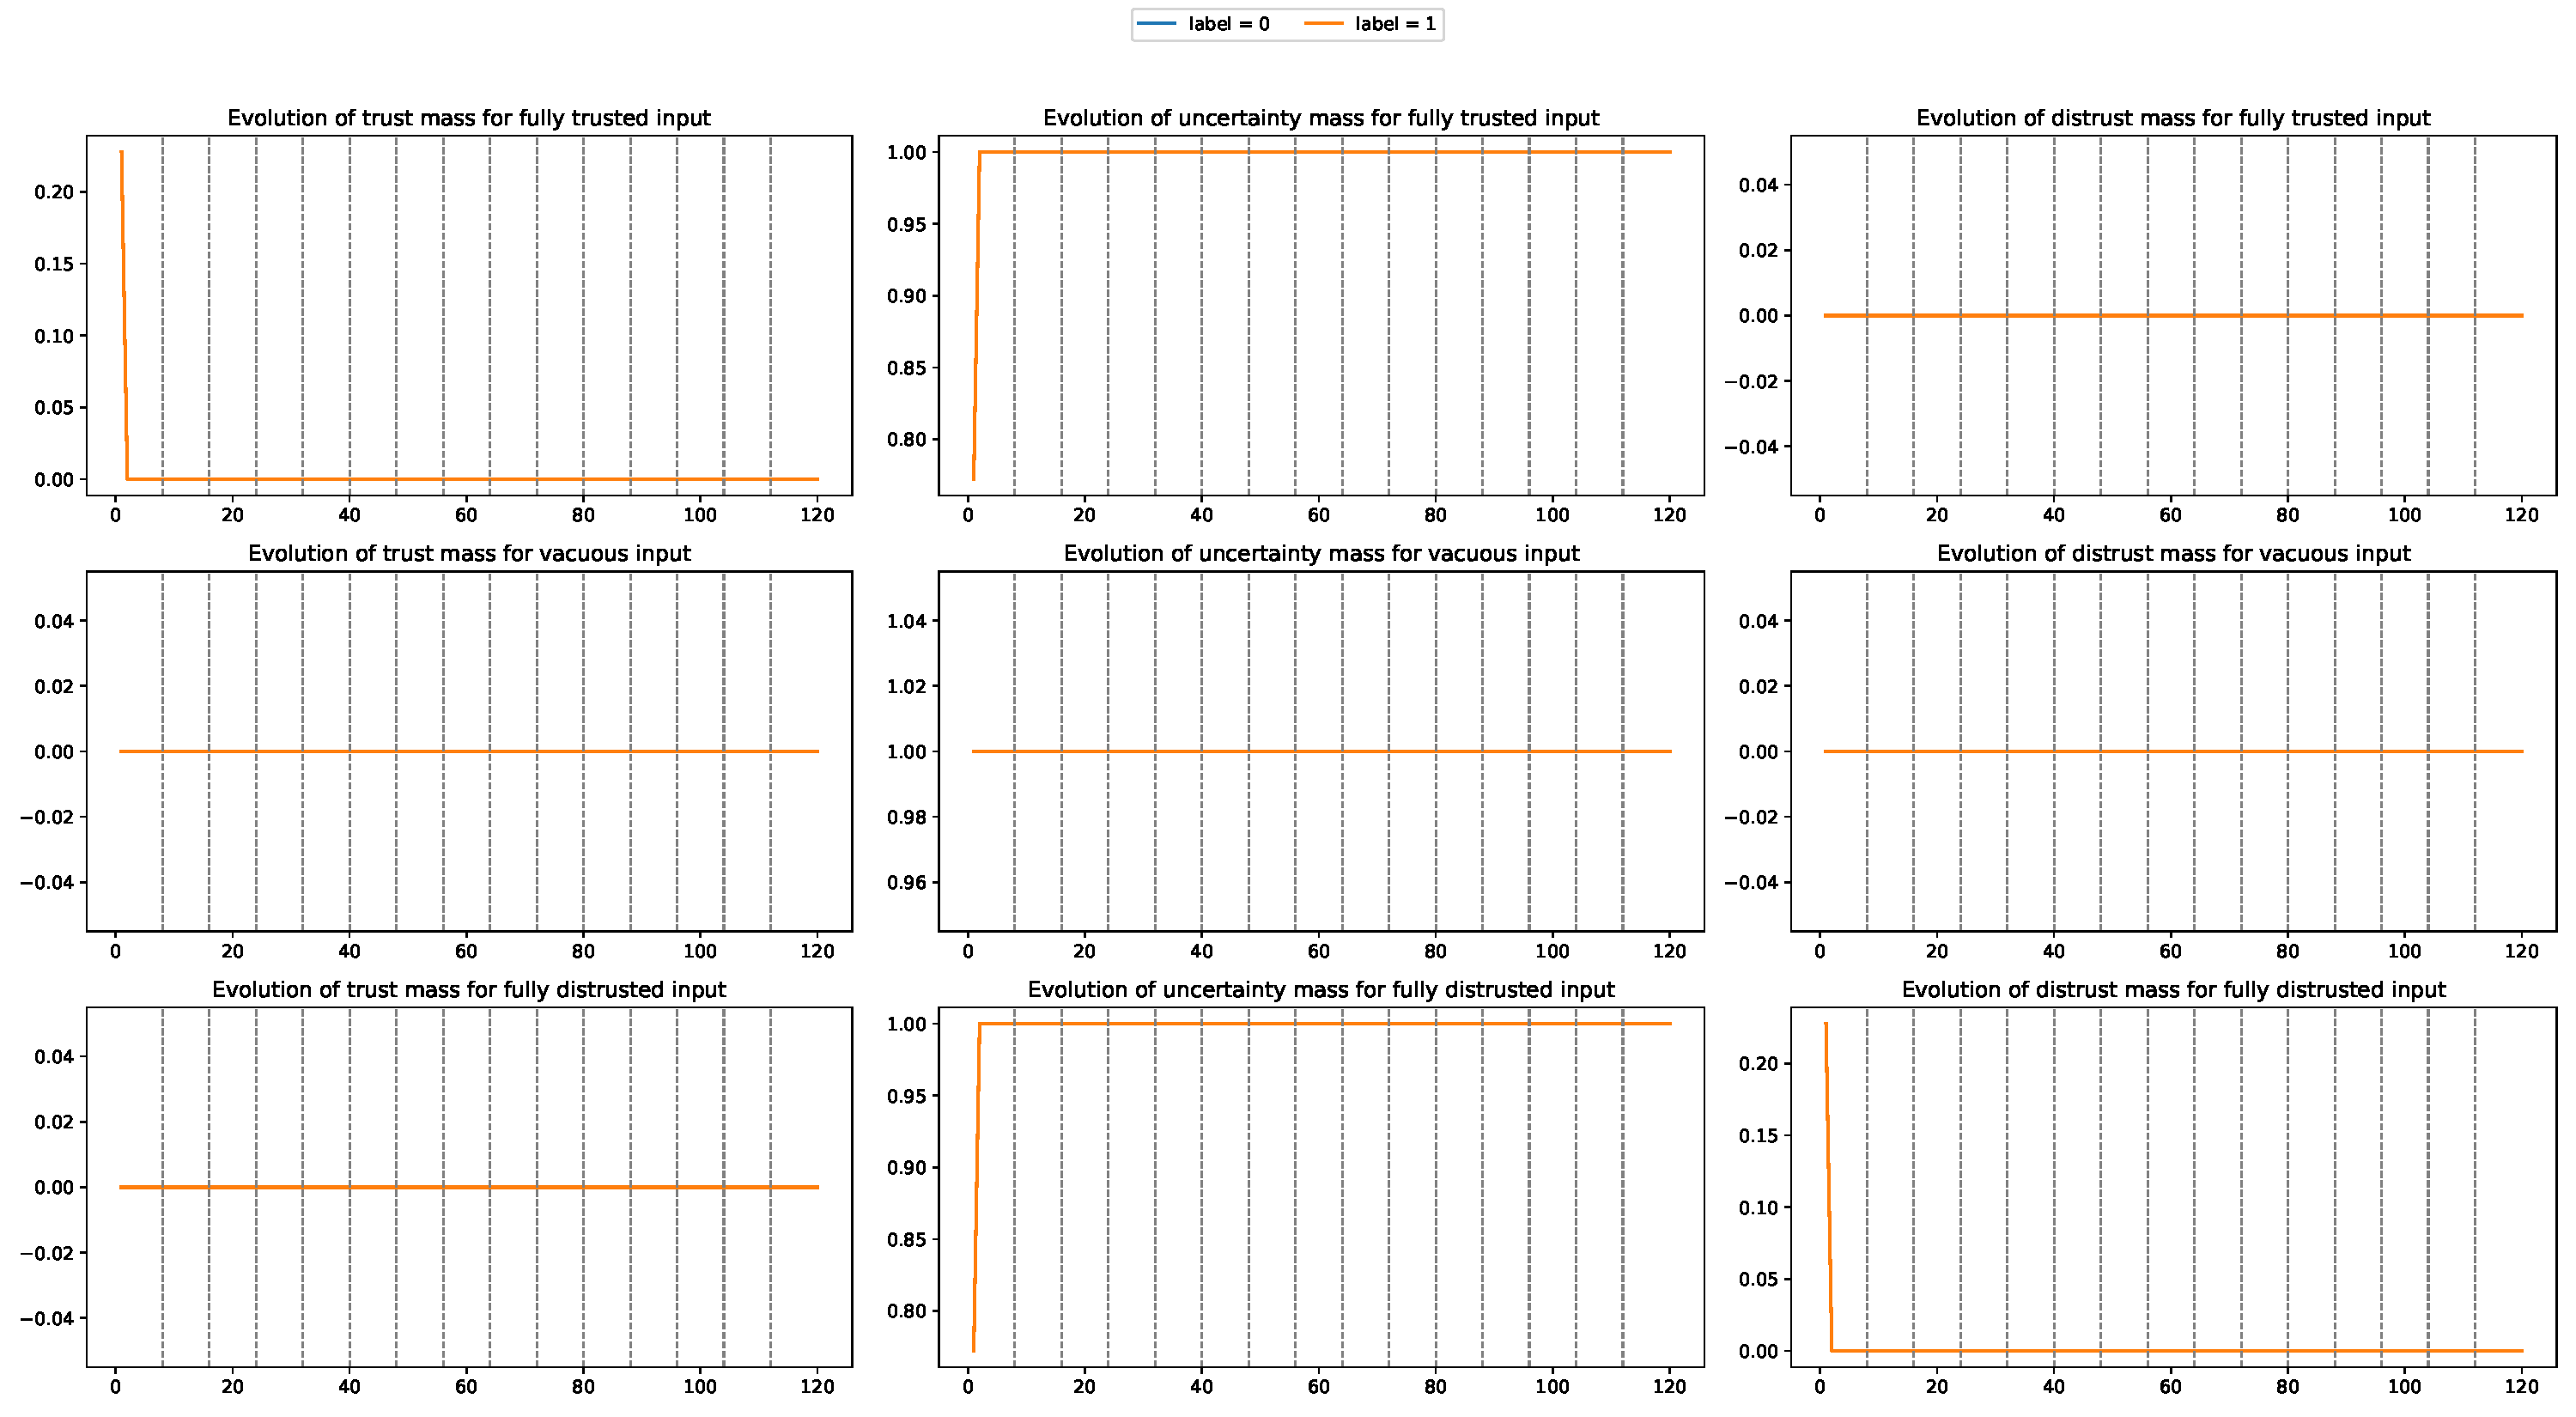
\includegraphics[width=0.8\textwidth]{latex/PTAS_Eval_cancer_16_distrust_distrust_eps_0.01_PathSize_None__plot_ptas.pdf}
\caption{cancer\_16\_distrust\_distrust, $\varepsilon$=0.01}
\end{figure}

\begin{figure}[htbp]
\centering
  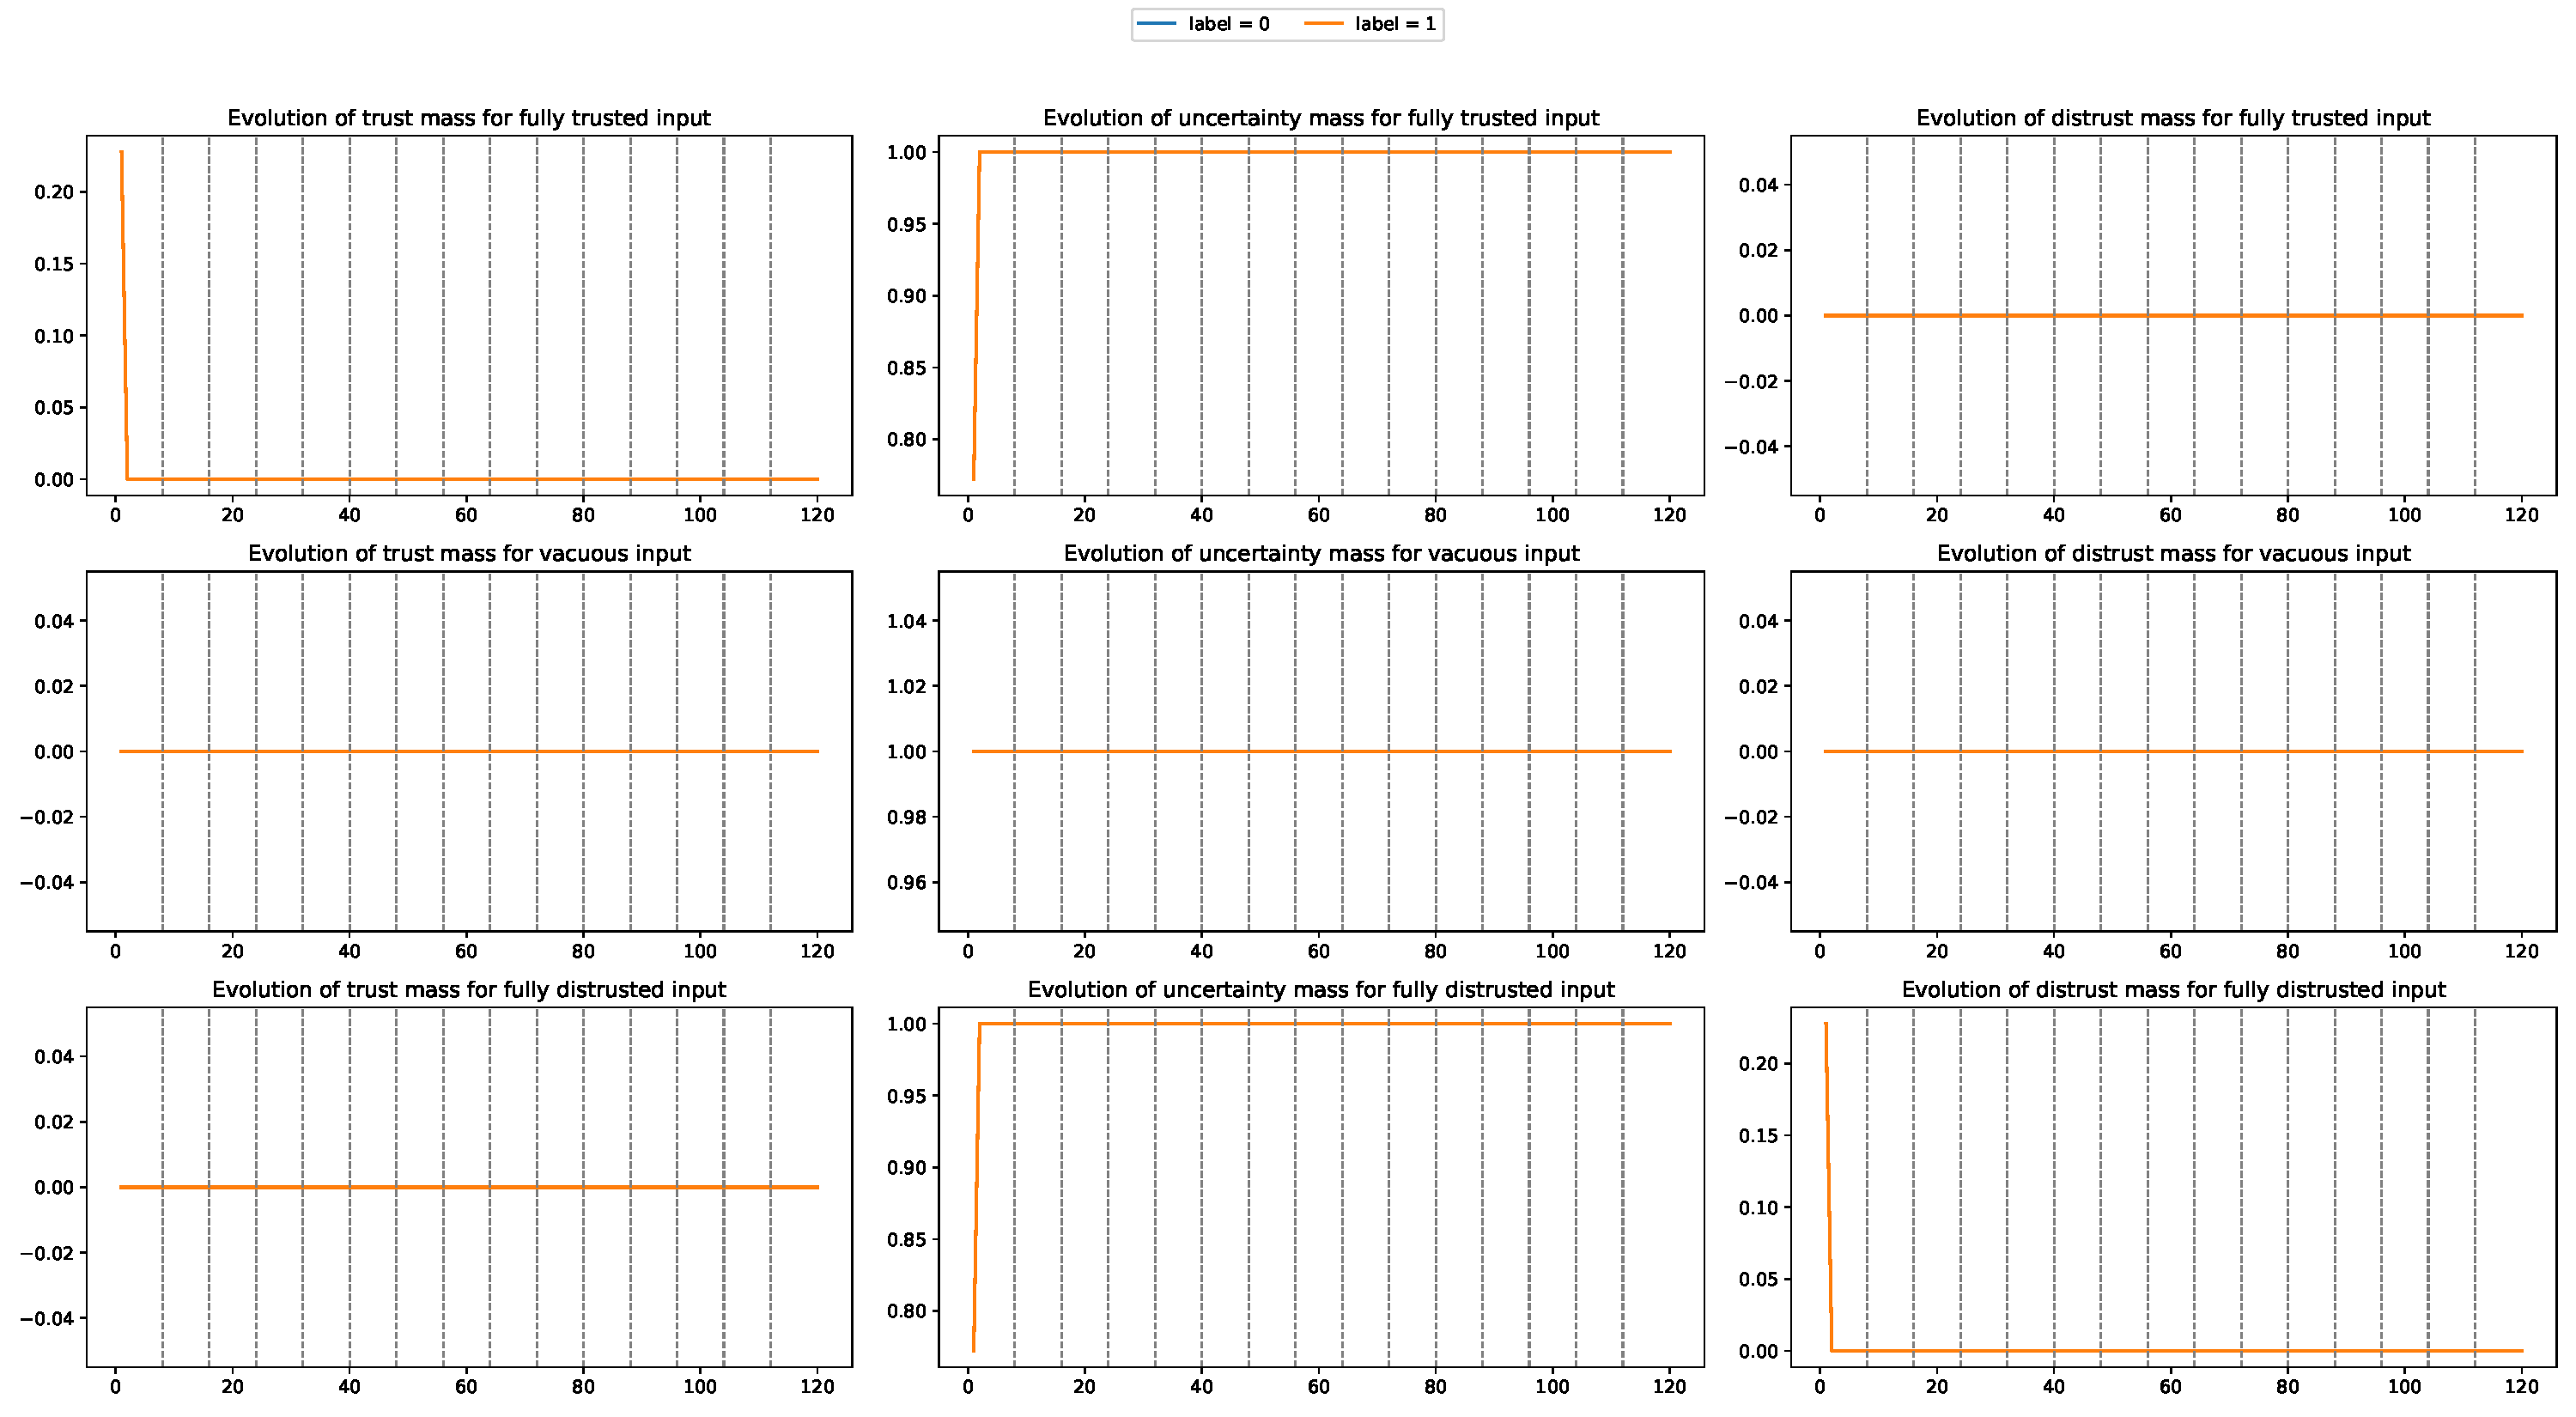
\includegraphics[width=0.8\textwidth]{latex/PTAS_Eval_cancer_16_distrust_distrust_eps_0.1_PathSize_None__plot_ptas.pdf}
\caption{cancer\_16\_distrust\_distrust, $\varepsilon$=0.1}
\end{figure}

\begin{figure}[htbp]
\centering
  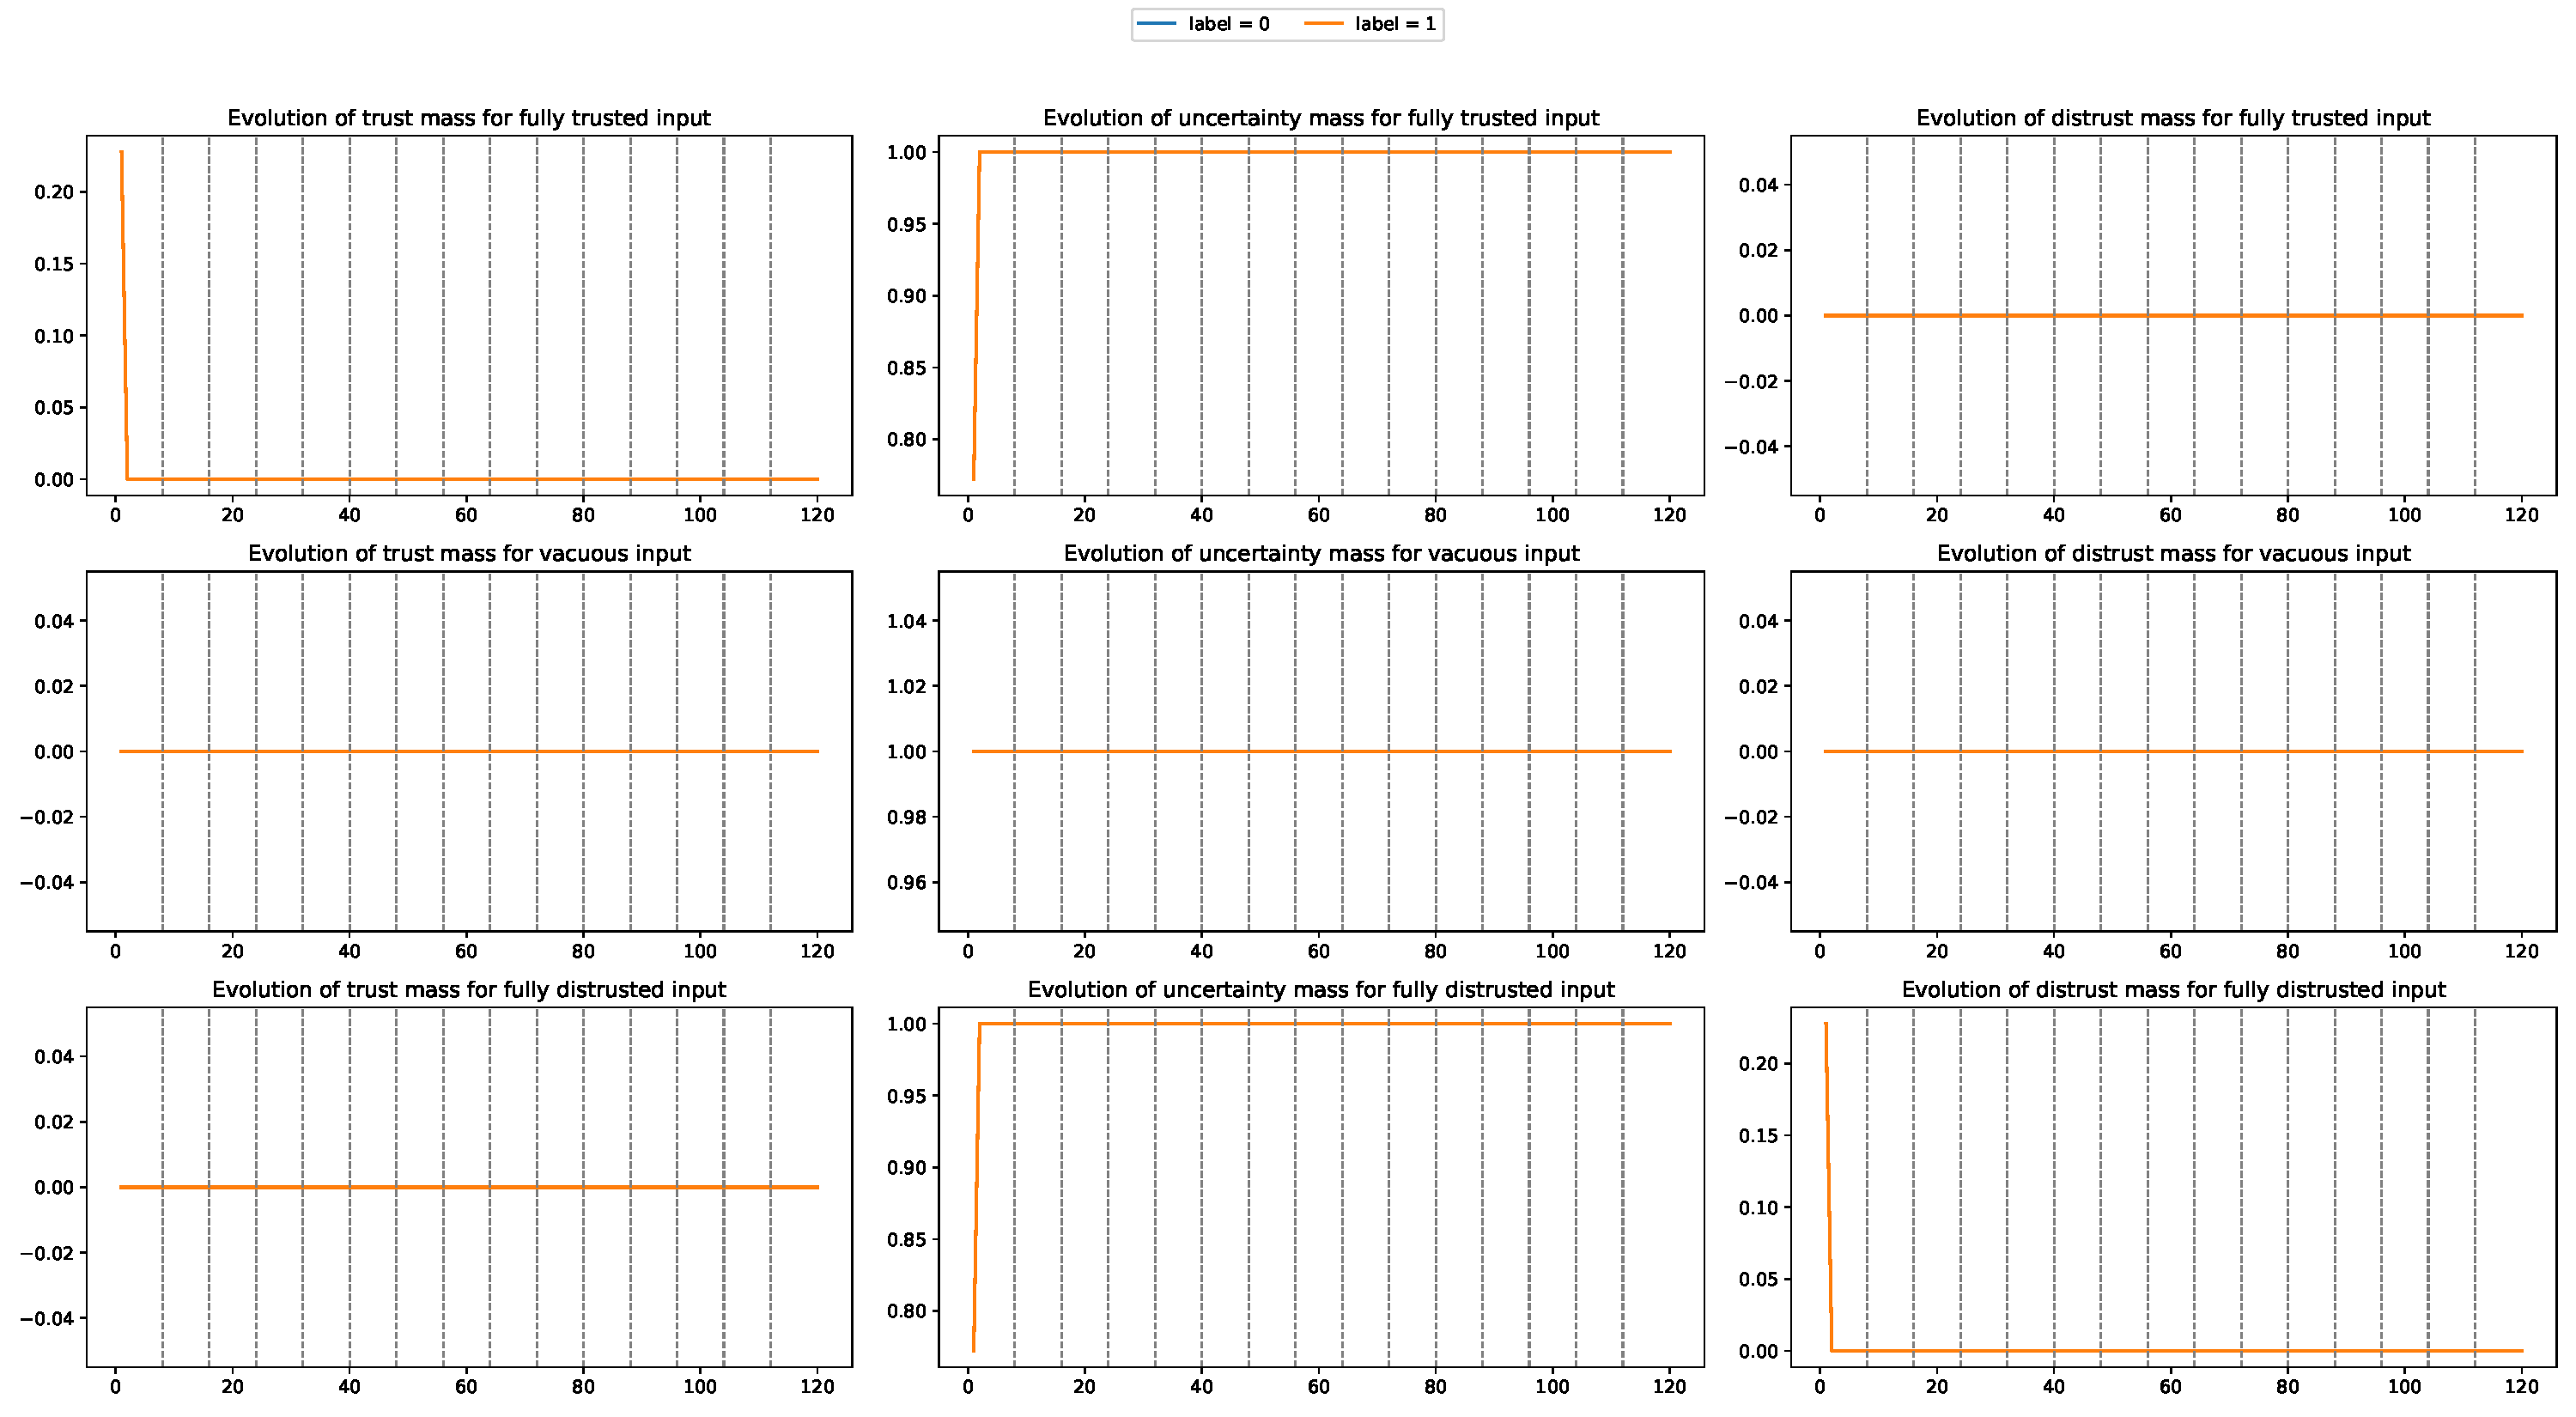
\includegraphics[width=0.8\textwidth]{latex/PTAS_Eval_cancer_16_distrust_distrust_eps_1_PathSize_None__plot_ptas.pdf}
\caption{cancer\_16\_distrust\_distrust, $\varepsilon$=1}
\end{figure}

\subsubsection{distrust -- trust}

\begin{figure}[htbp]
\centering
  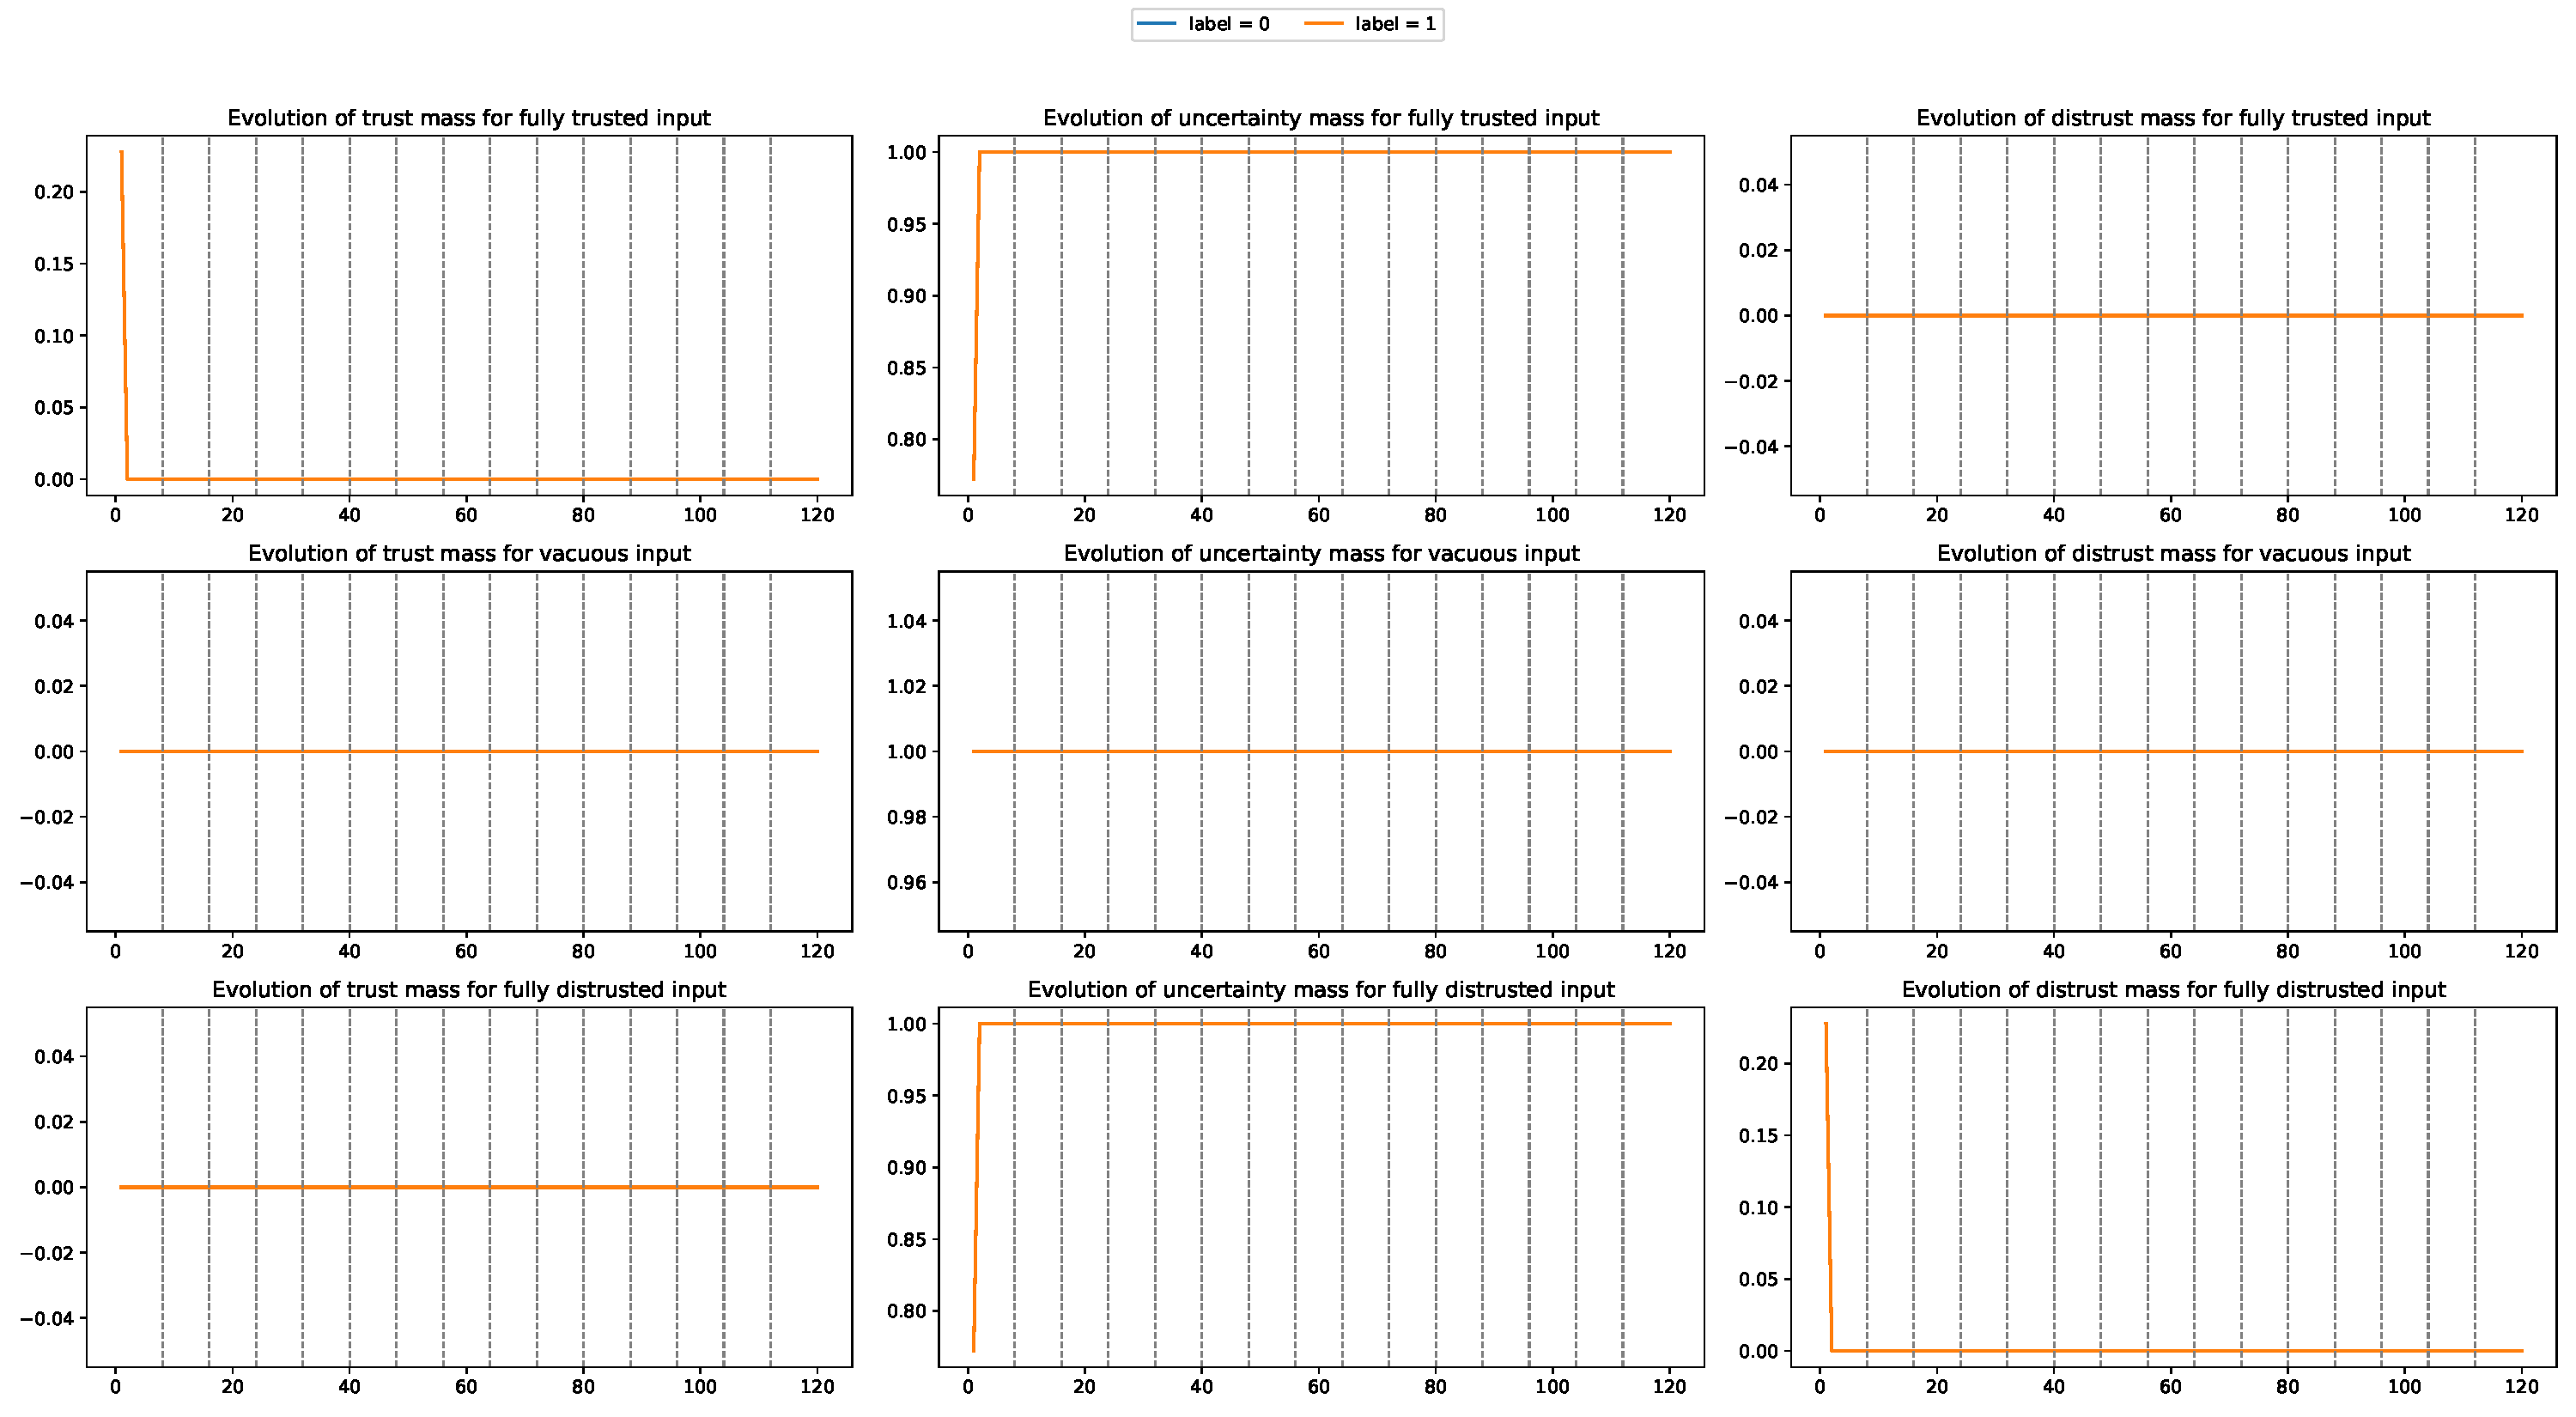
\includegraphics[width=0.8\textwidth]{latex/PTAS_Eval_cancer_16_distrust_trust_eps_0.001_PathSize_None__plot_ptas.pdf}
\caption{cancer\_16\_distrust\_trust, $\varepsilon$=0.001}
\end{figure}

\begin{figure}[htbp]
\centering
  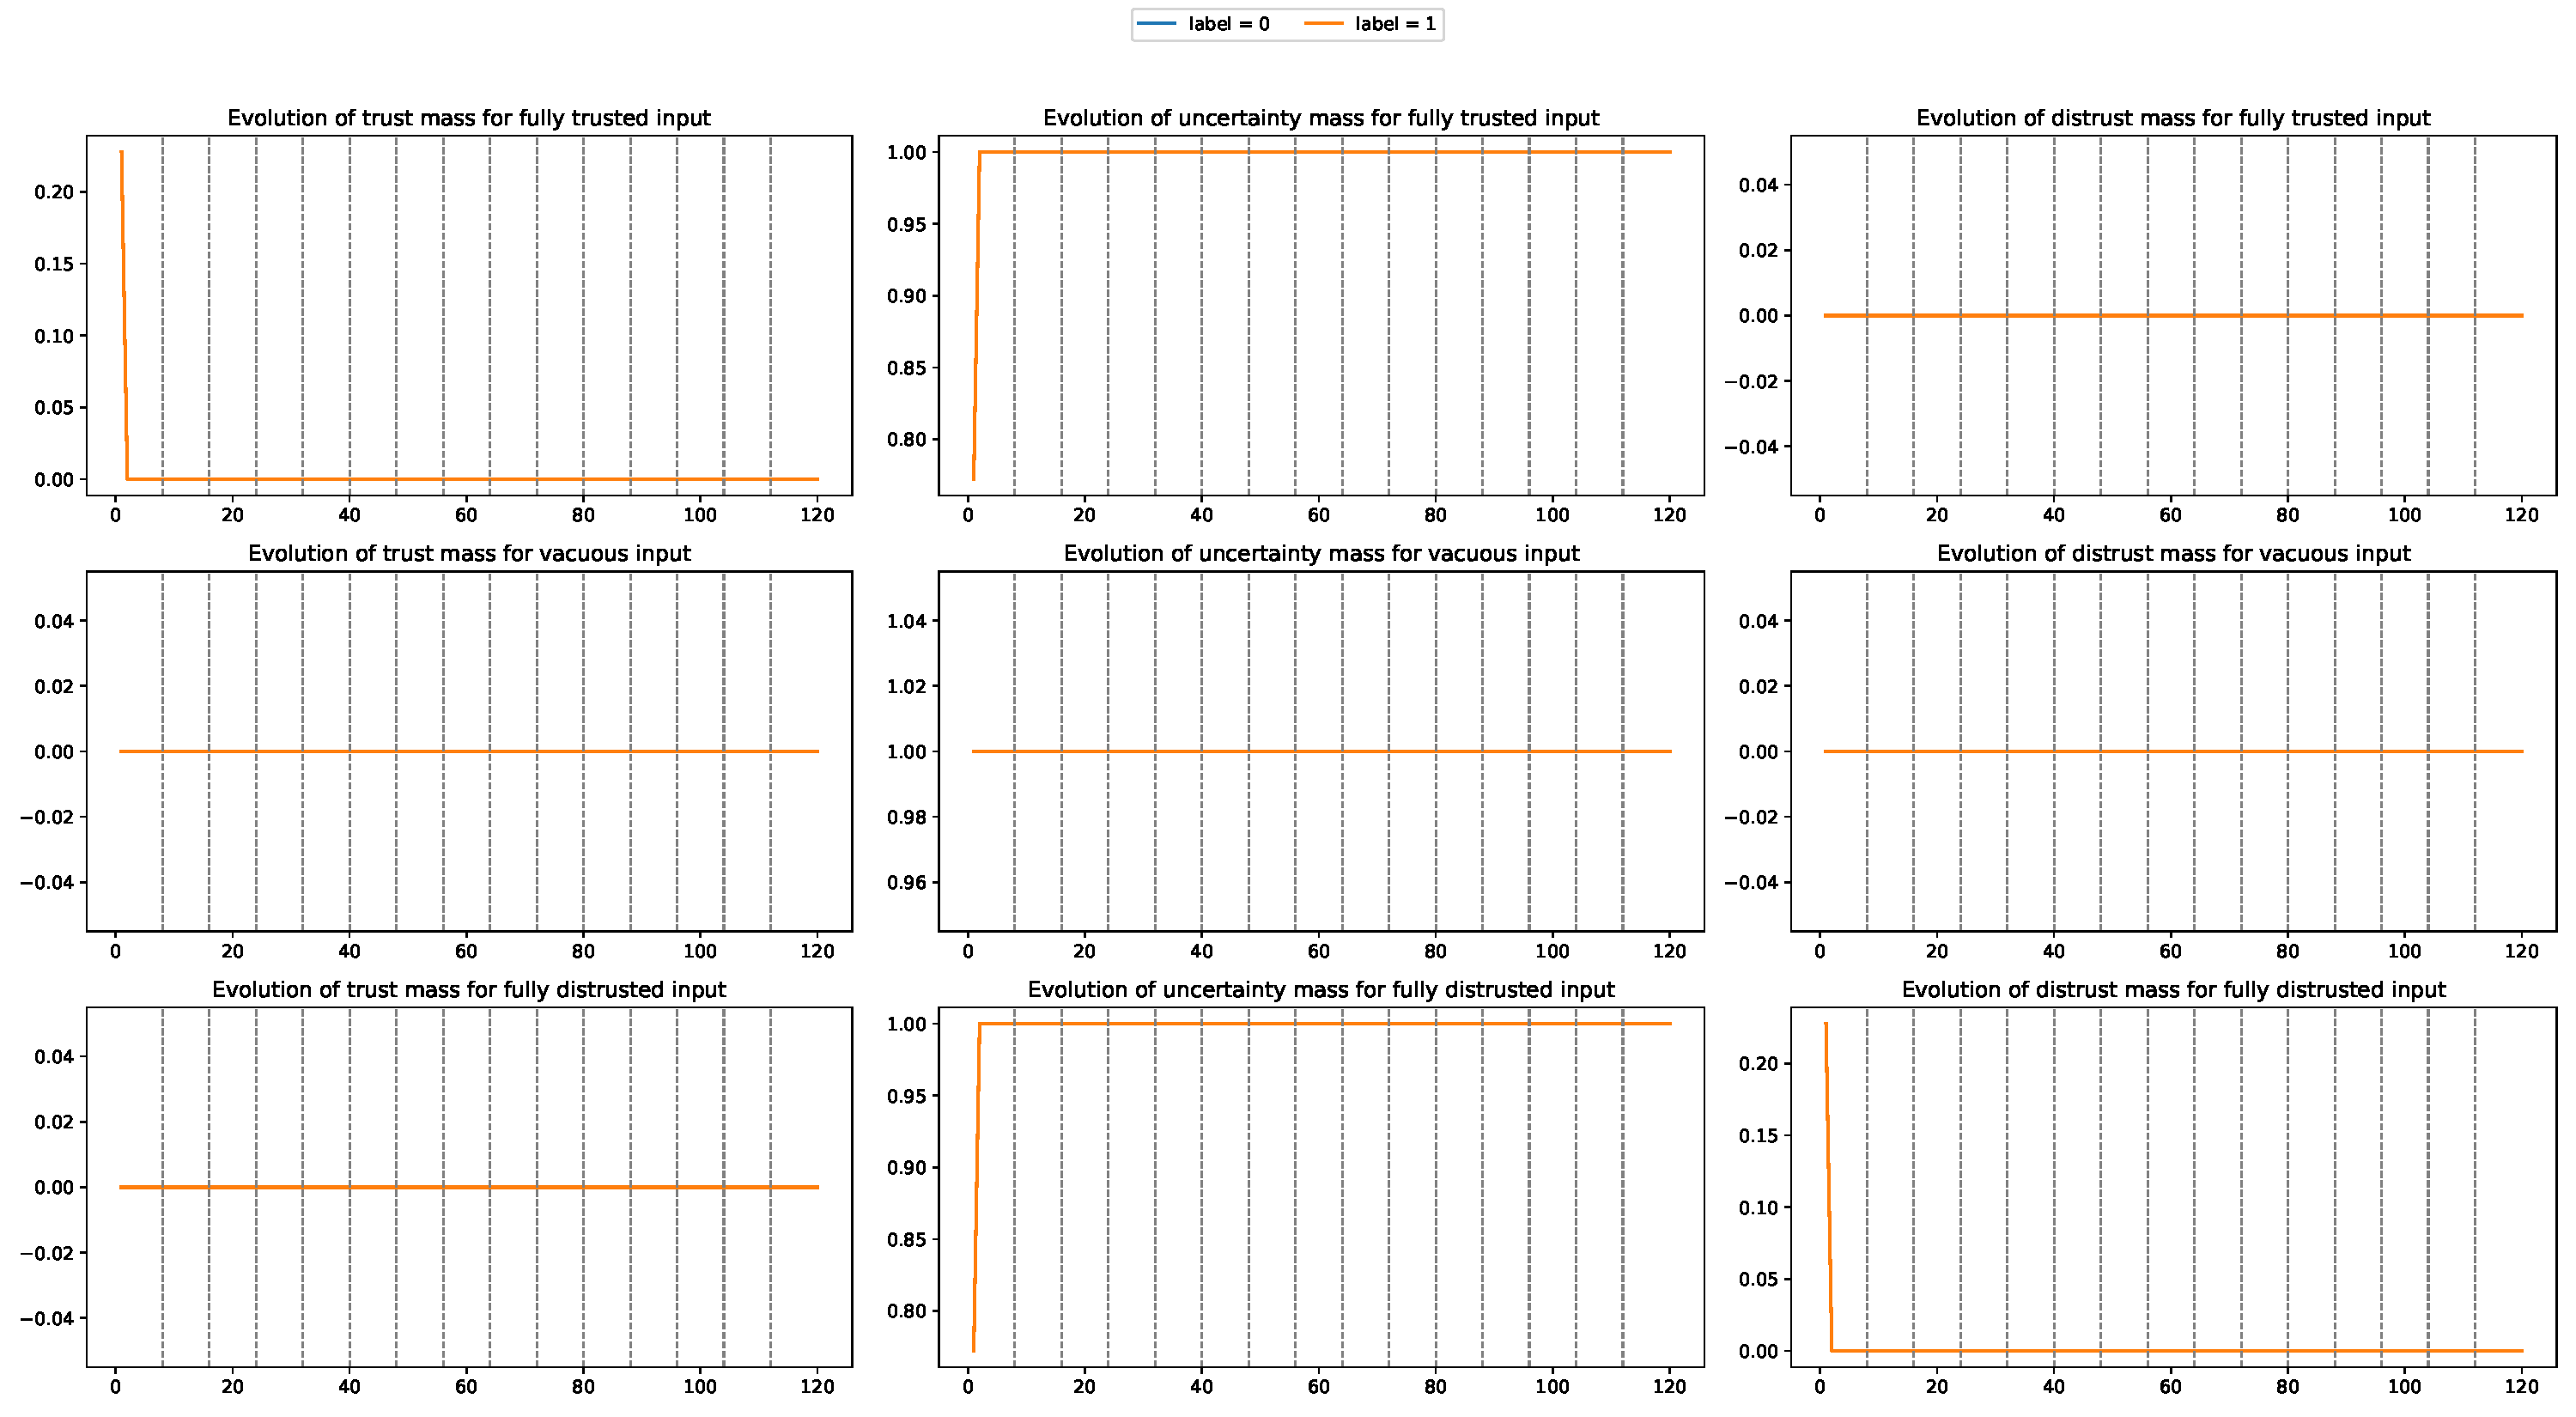
\includegraphics[width=0.8\textwidth]{latex/PTAS_Eval_cancer_16_distrust_trust_eps_0.01_PathSize_None__plot_ptas.pdf}
\caption{cancer\_16\_distrust\_trust, $\varepsilon$=0.01}
\end{figure}

\begin{figure}[htbp]
\centering
  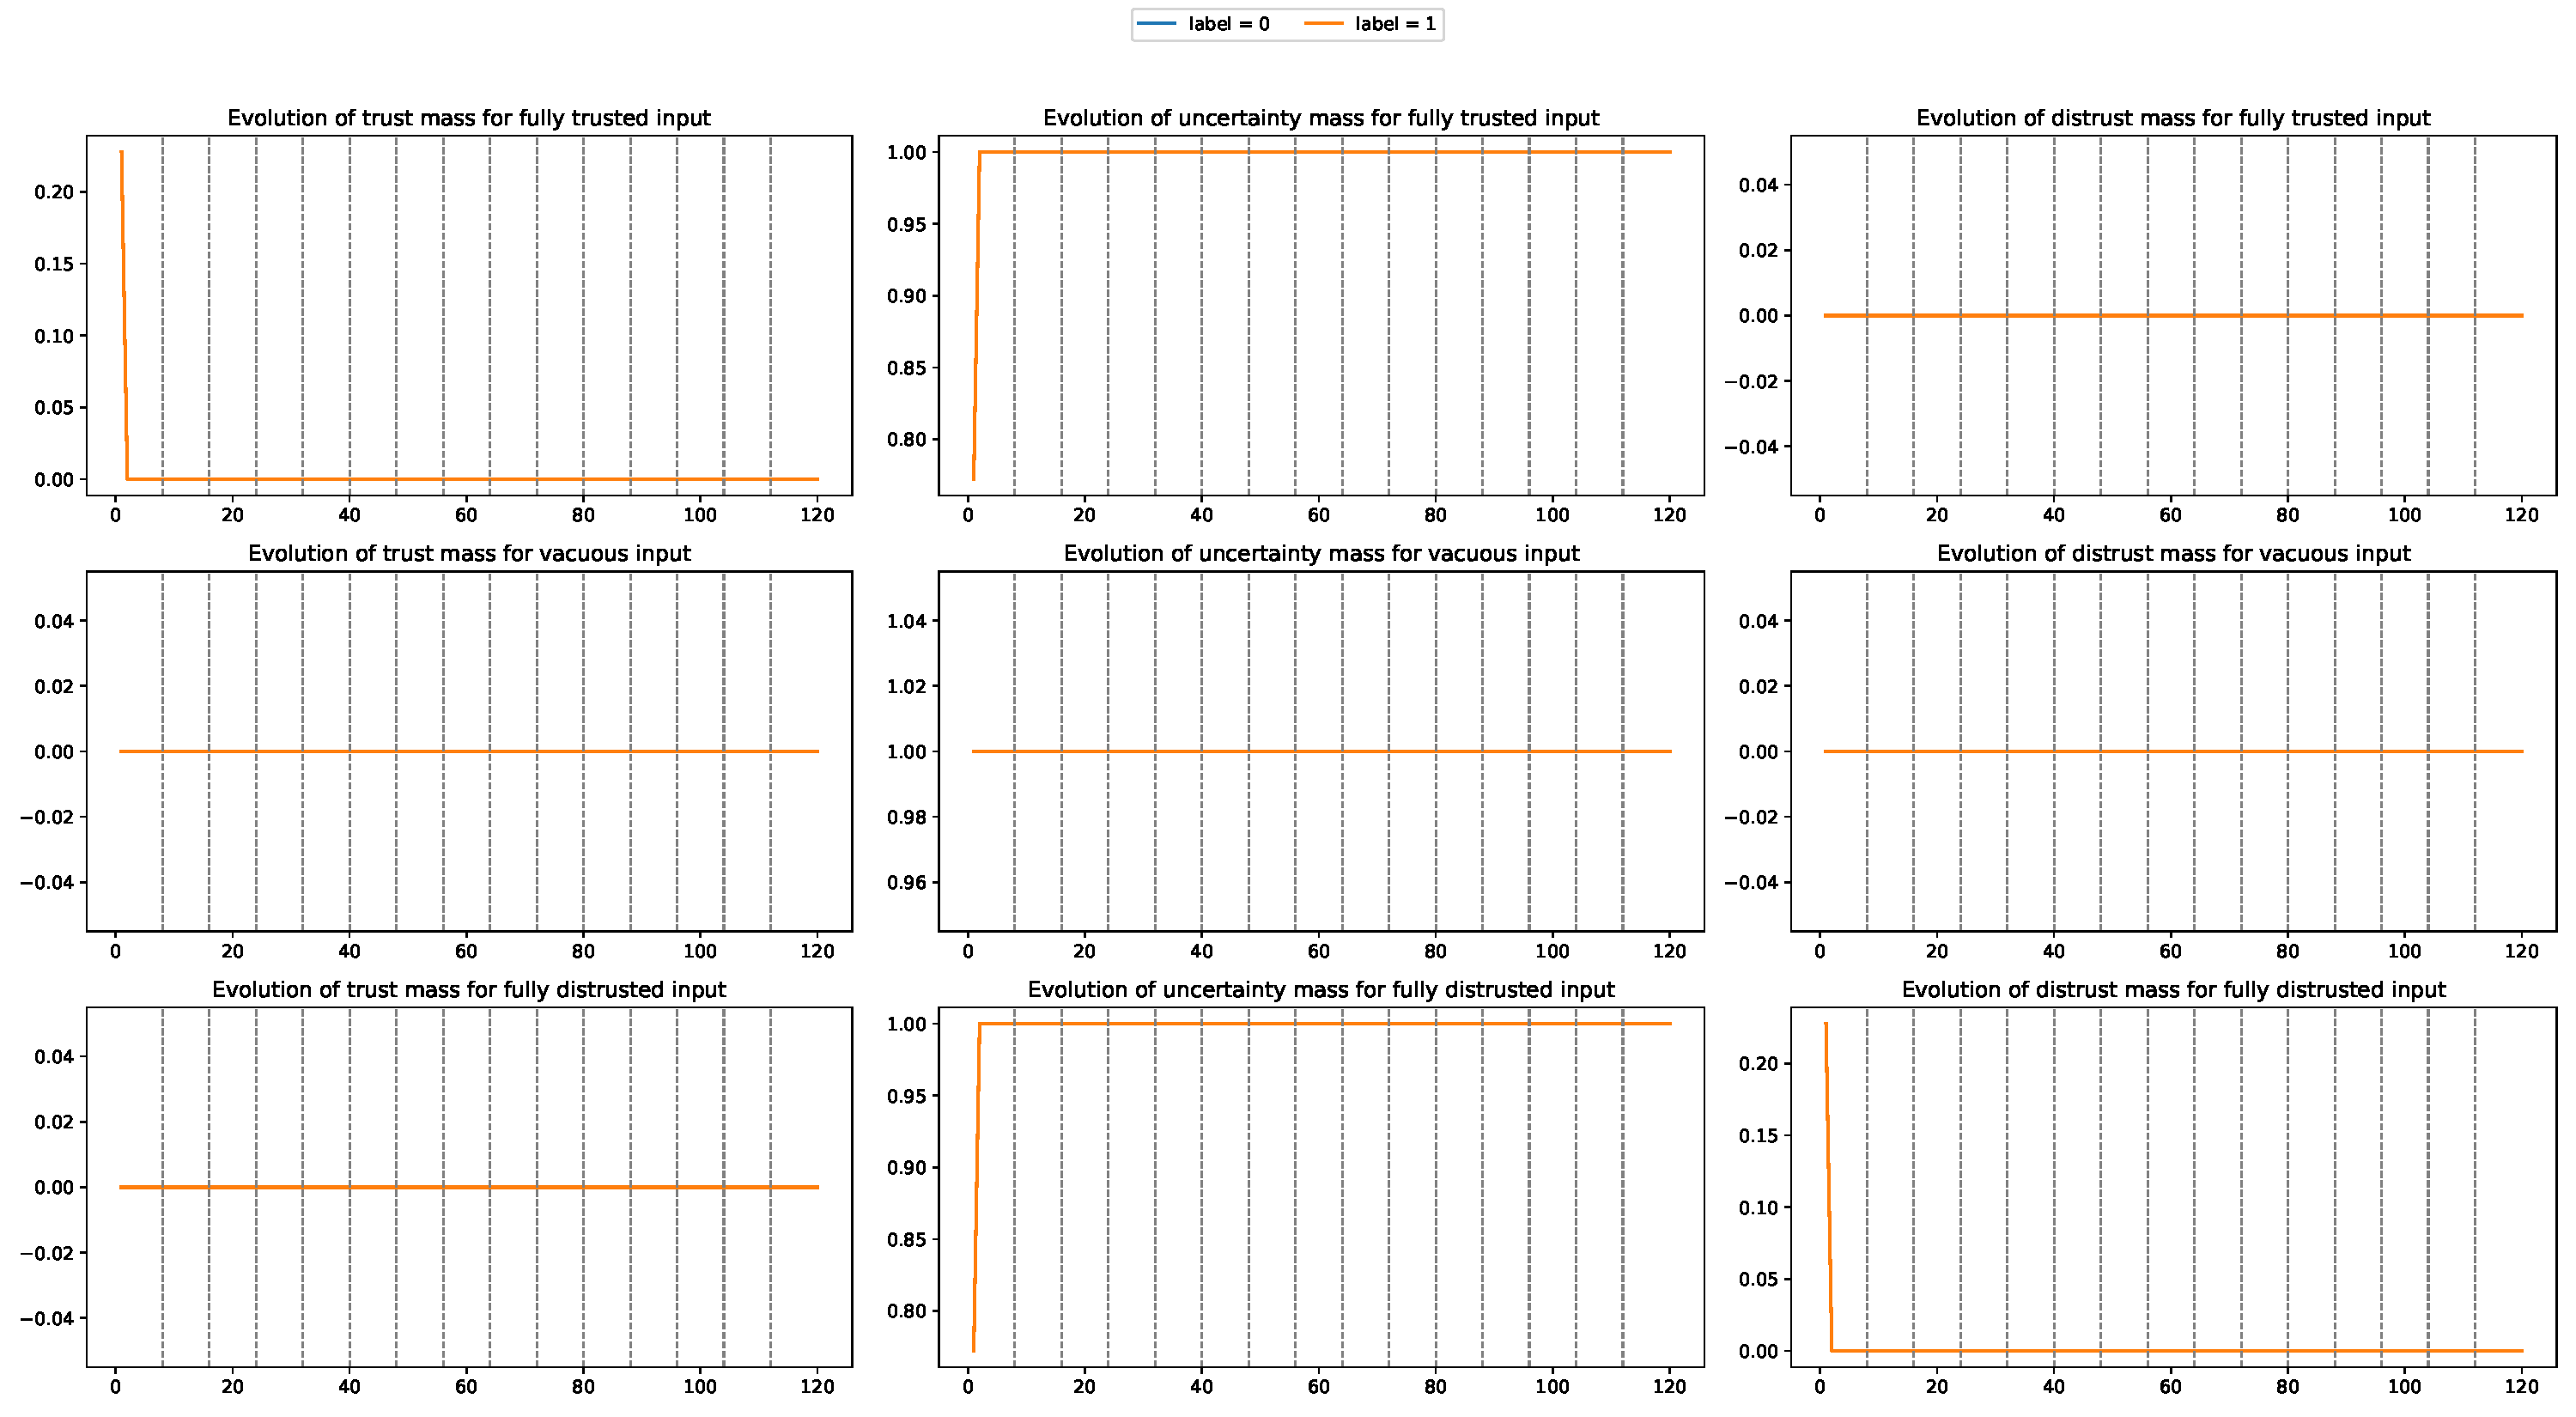
\includegraphics[width=0.8\textwidth]{latex/PTAS_Eval_cancer_16_distrust_trust_eps_0.1_PathSize_None__plot_ptas.pdf}
\caption{cancer\_16\_distrust\_trust, $\varepsilon$=0.1}
\end{figure}

\begin{figure}[htbp]
\centering
  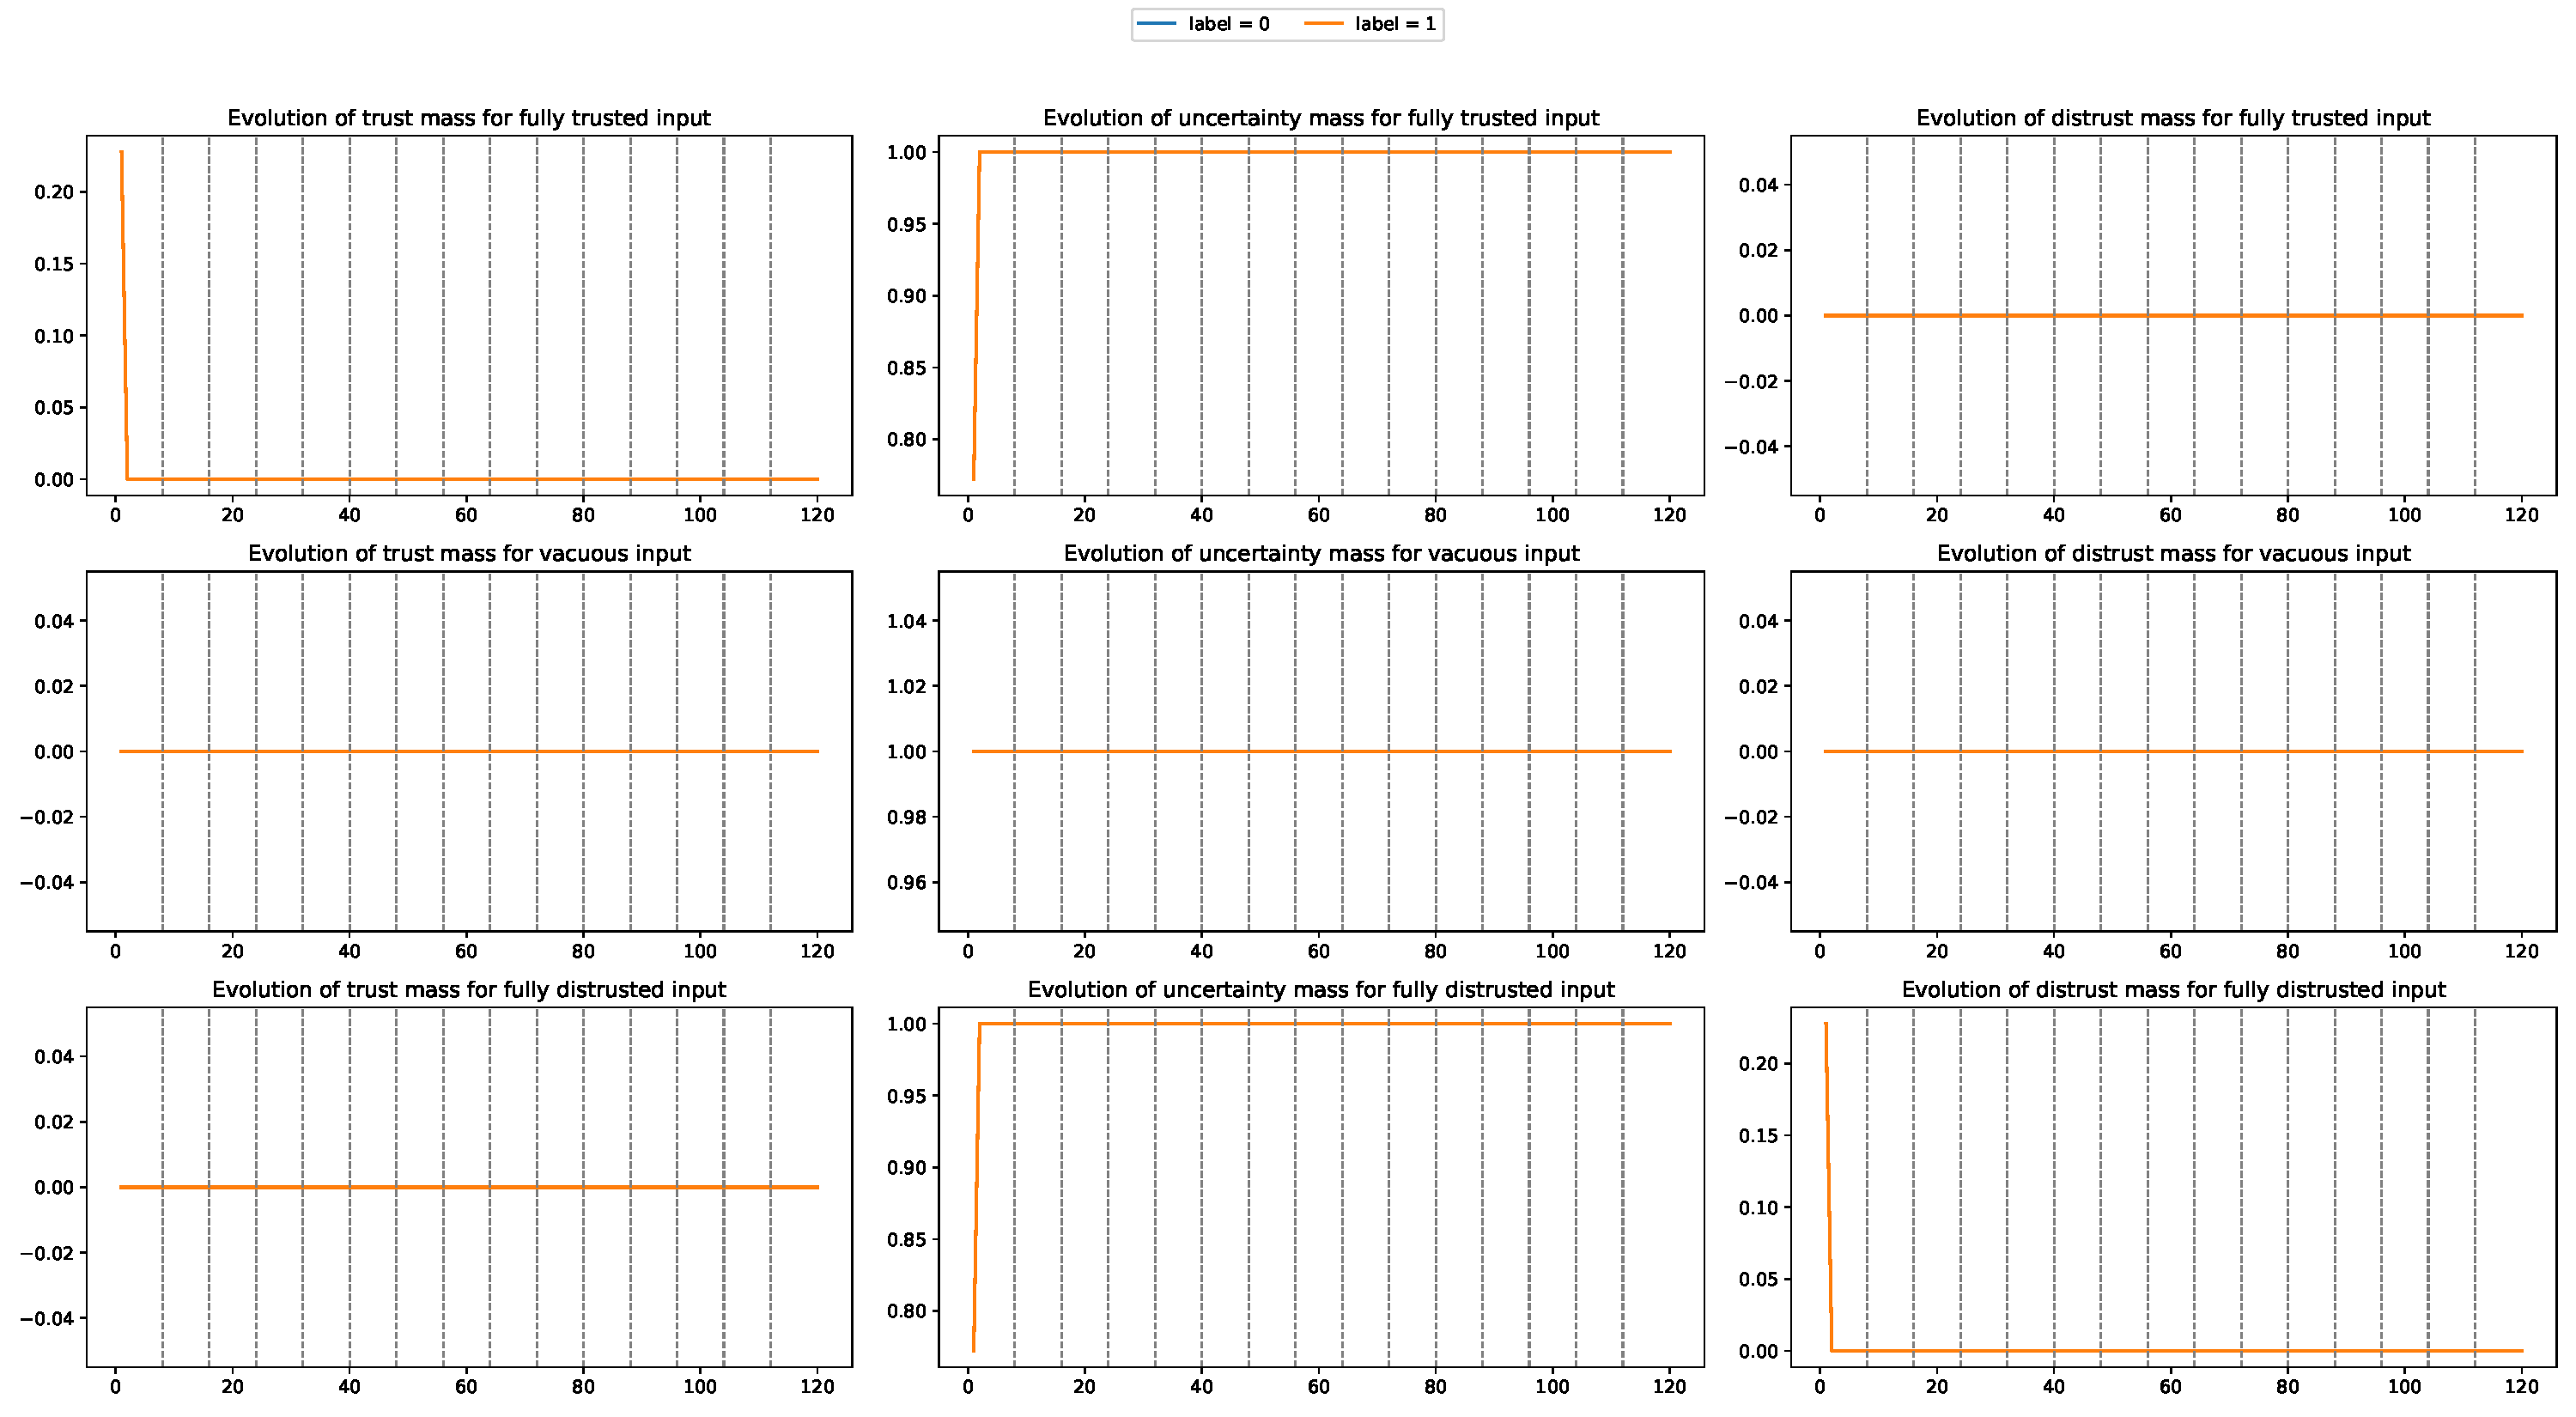
\includegraphics[width=0.8\textwidth]{latex/PTAS_Eval_cancer_16_distrust_trust_eps_1_PathSize_None__plot_ptas.pdf}
\caption{cancer\_16\_distrust\_trust, $\varepsilon$=1}
\end{figure}

\subsubsection{distrust -- vacuous}

\begin{figure}[htbp]
\centering
  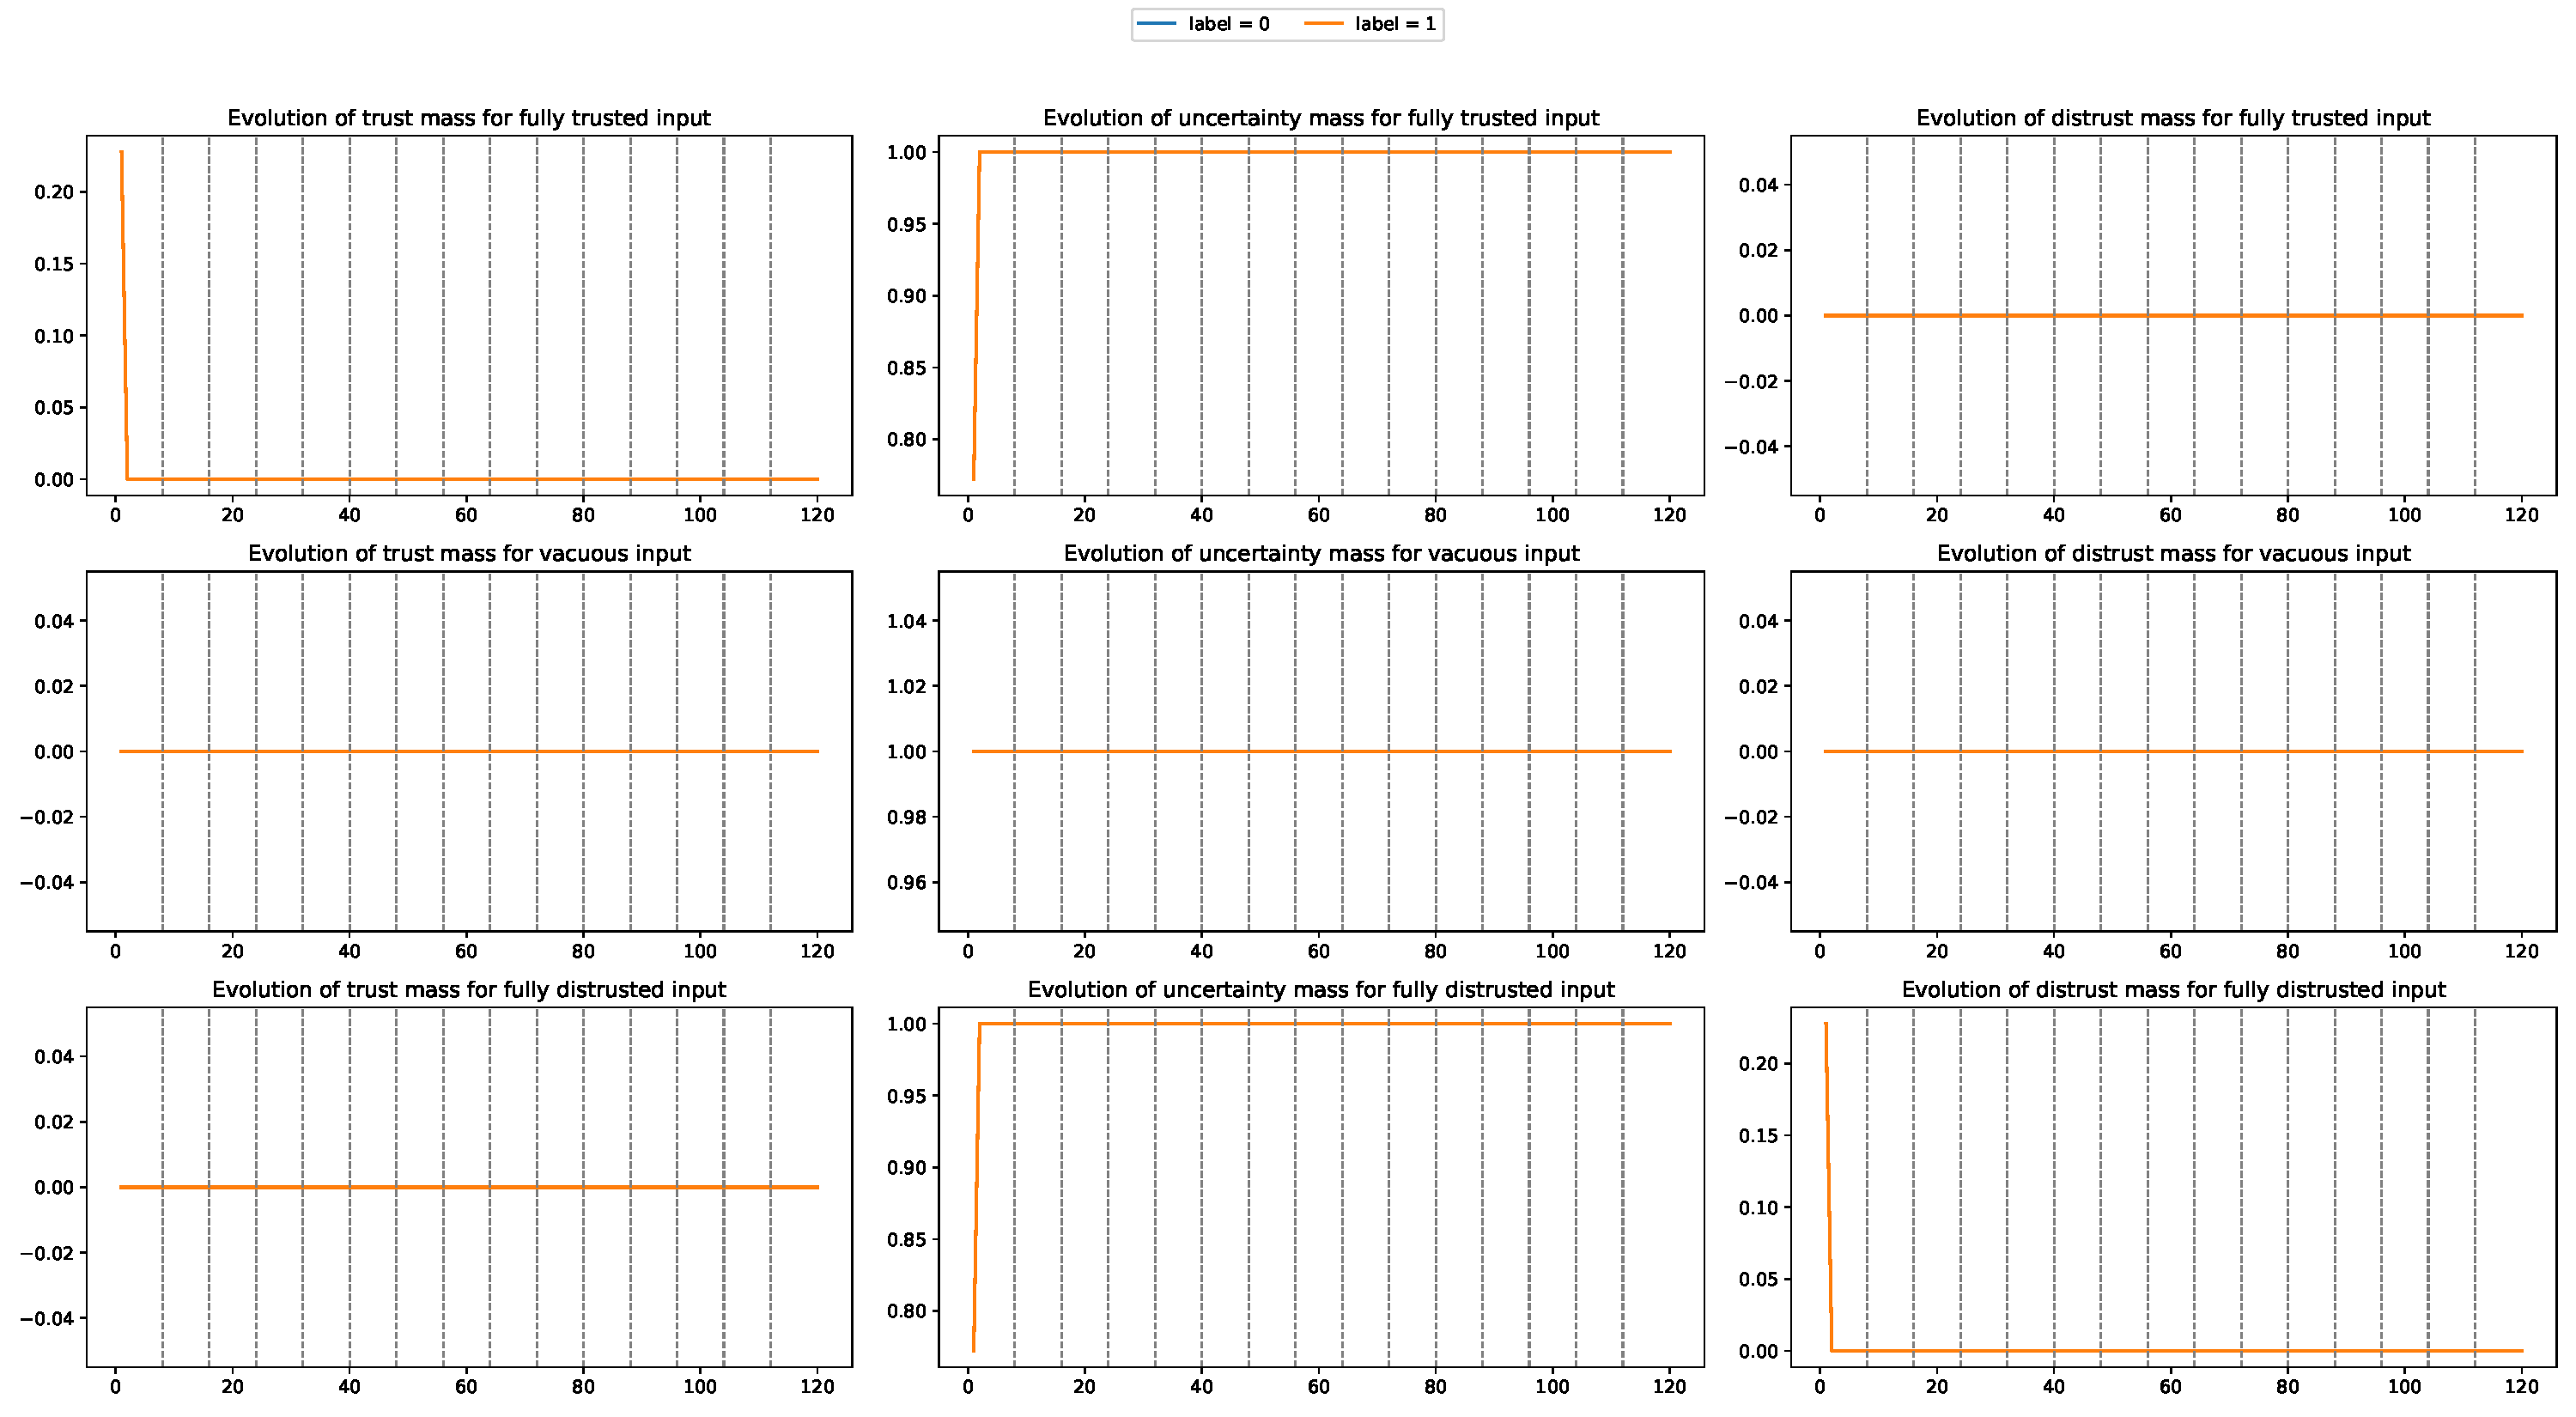
\includegraphics[width=0.8\textwidth]{latex/PTAS_Eval_cancer_16_distrust_vacuous_eps_0.001_PathSize_None__plot_ptas.pdf}
\caption{cancer\_16\_distrust\_vacuous, $\varepsilon$=0.001}
\end{figure}

\begin{figure}[htbp]
\centering
  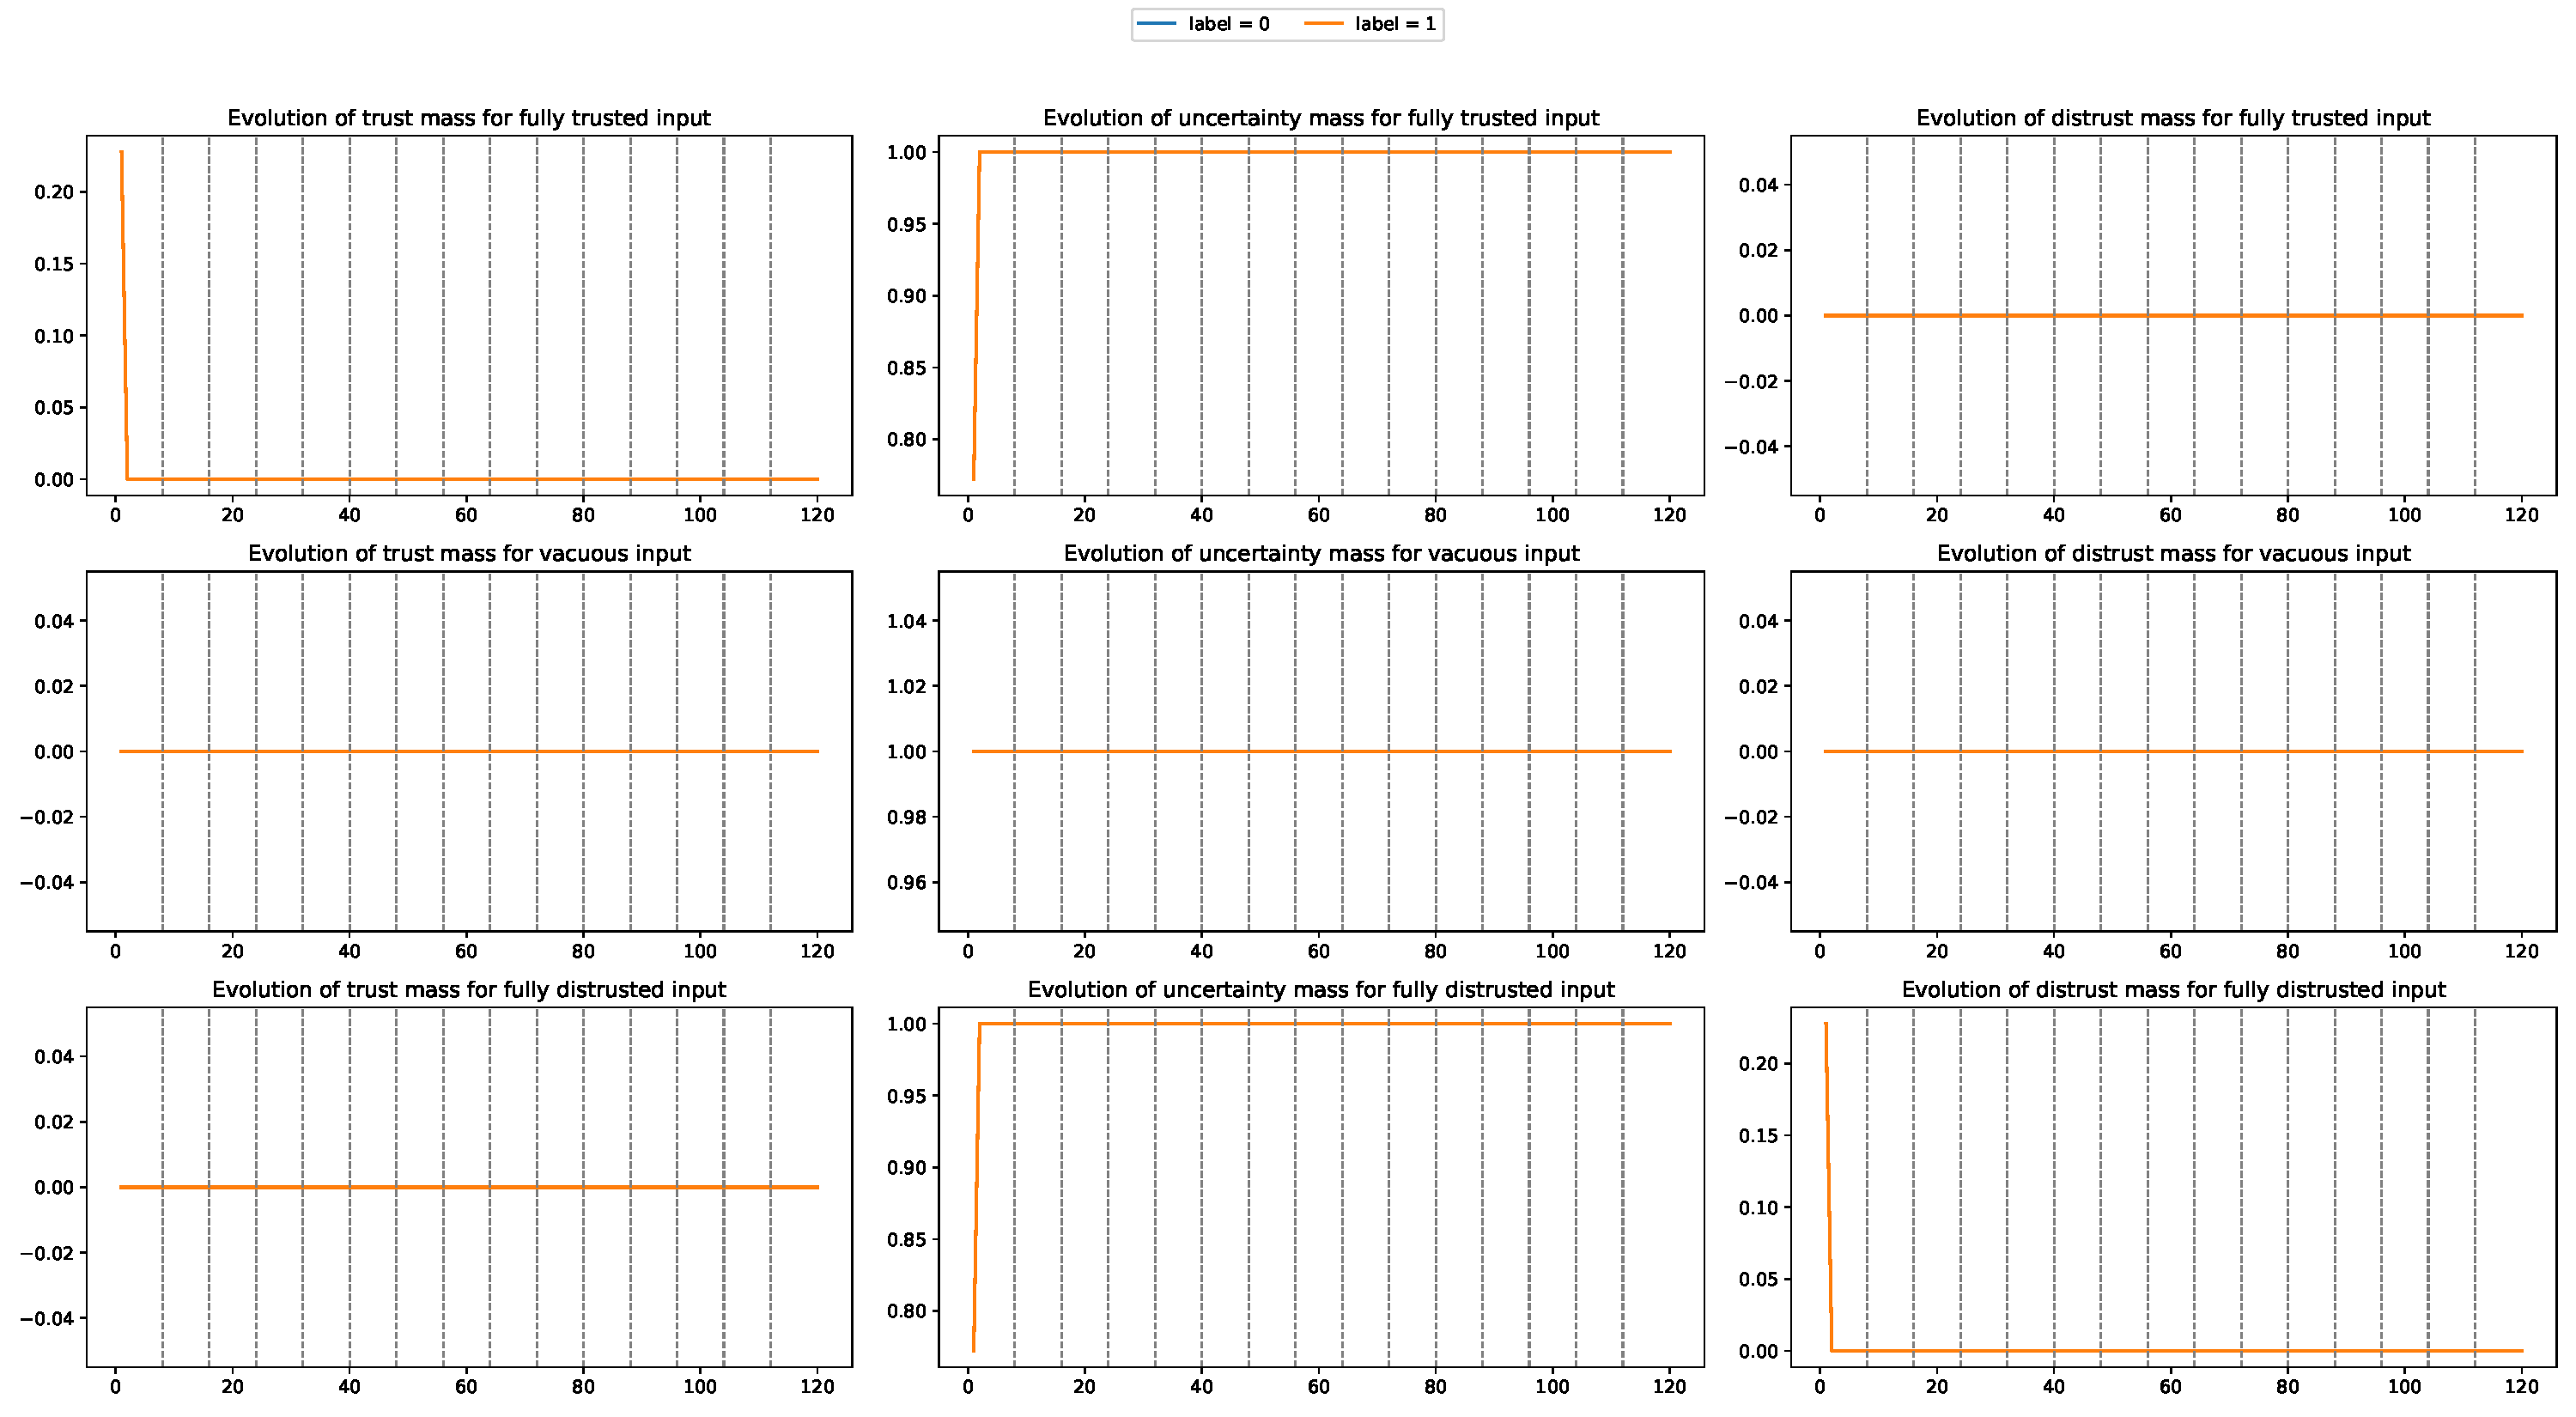
\includegraphics[width=0.8\textwidth]{latex/PTAS_Eval_cancer_16_distrust_vacuous_eps_0.01_PathSize_None__plot_ptas.pdf}
\caption{cancer\_16\_distrust\_vacuous, $\varepsilon$=0.01}
\end{figure}

\begin{figure}[htbp]
\centering
  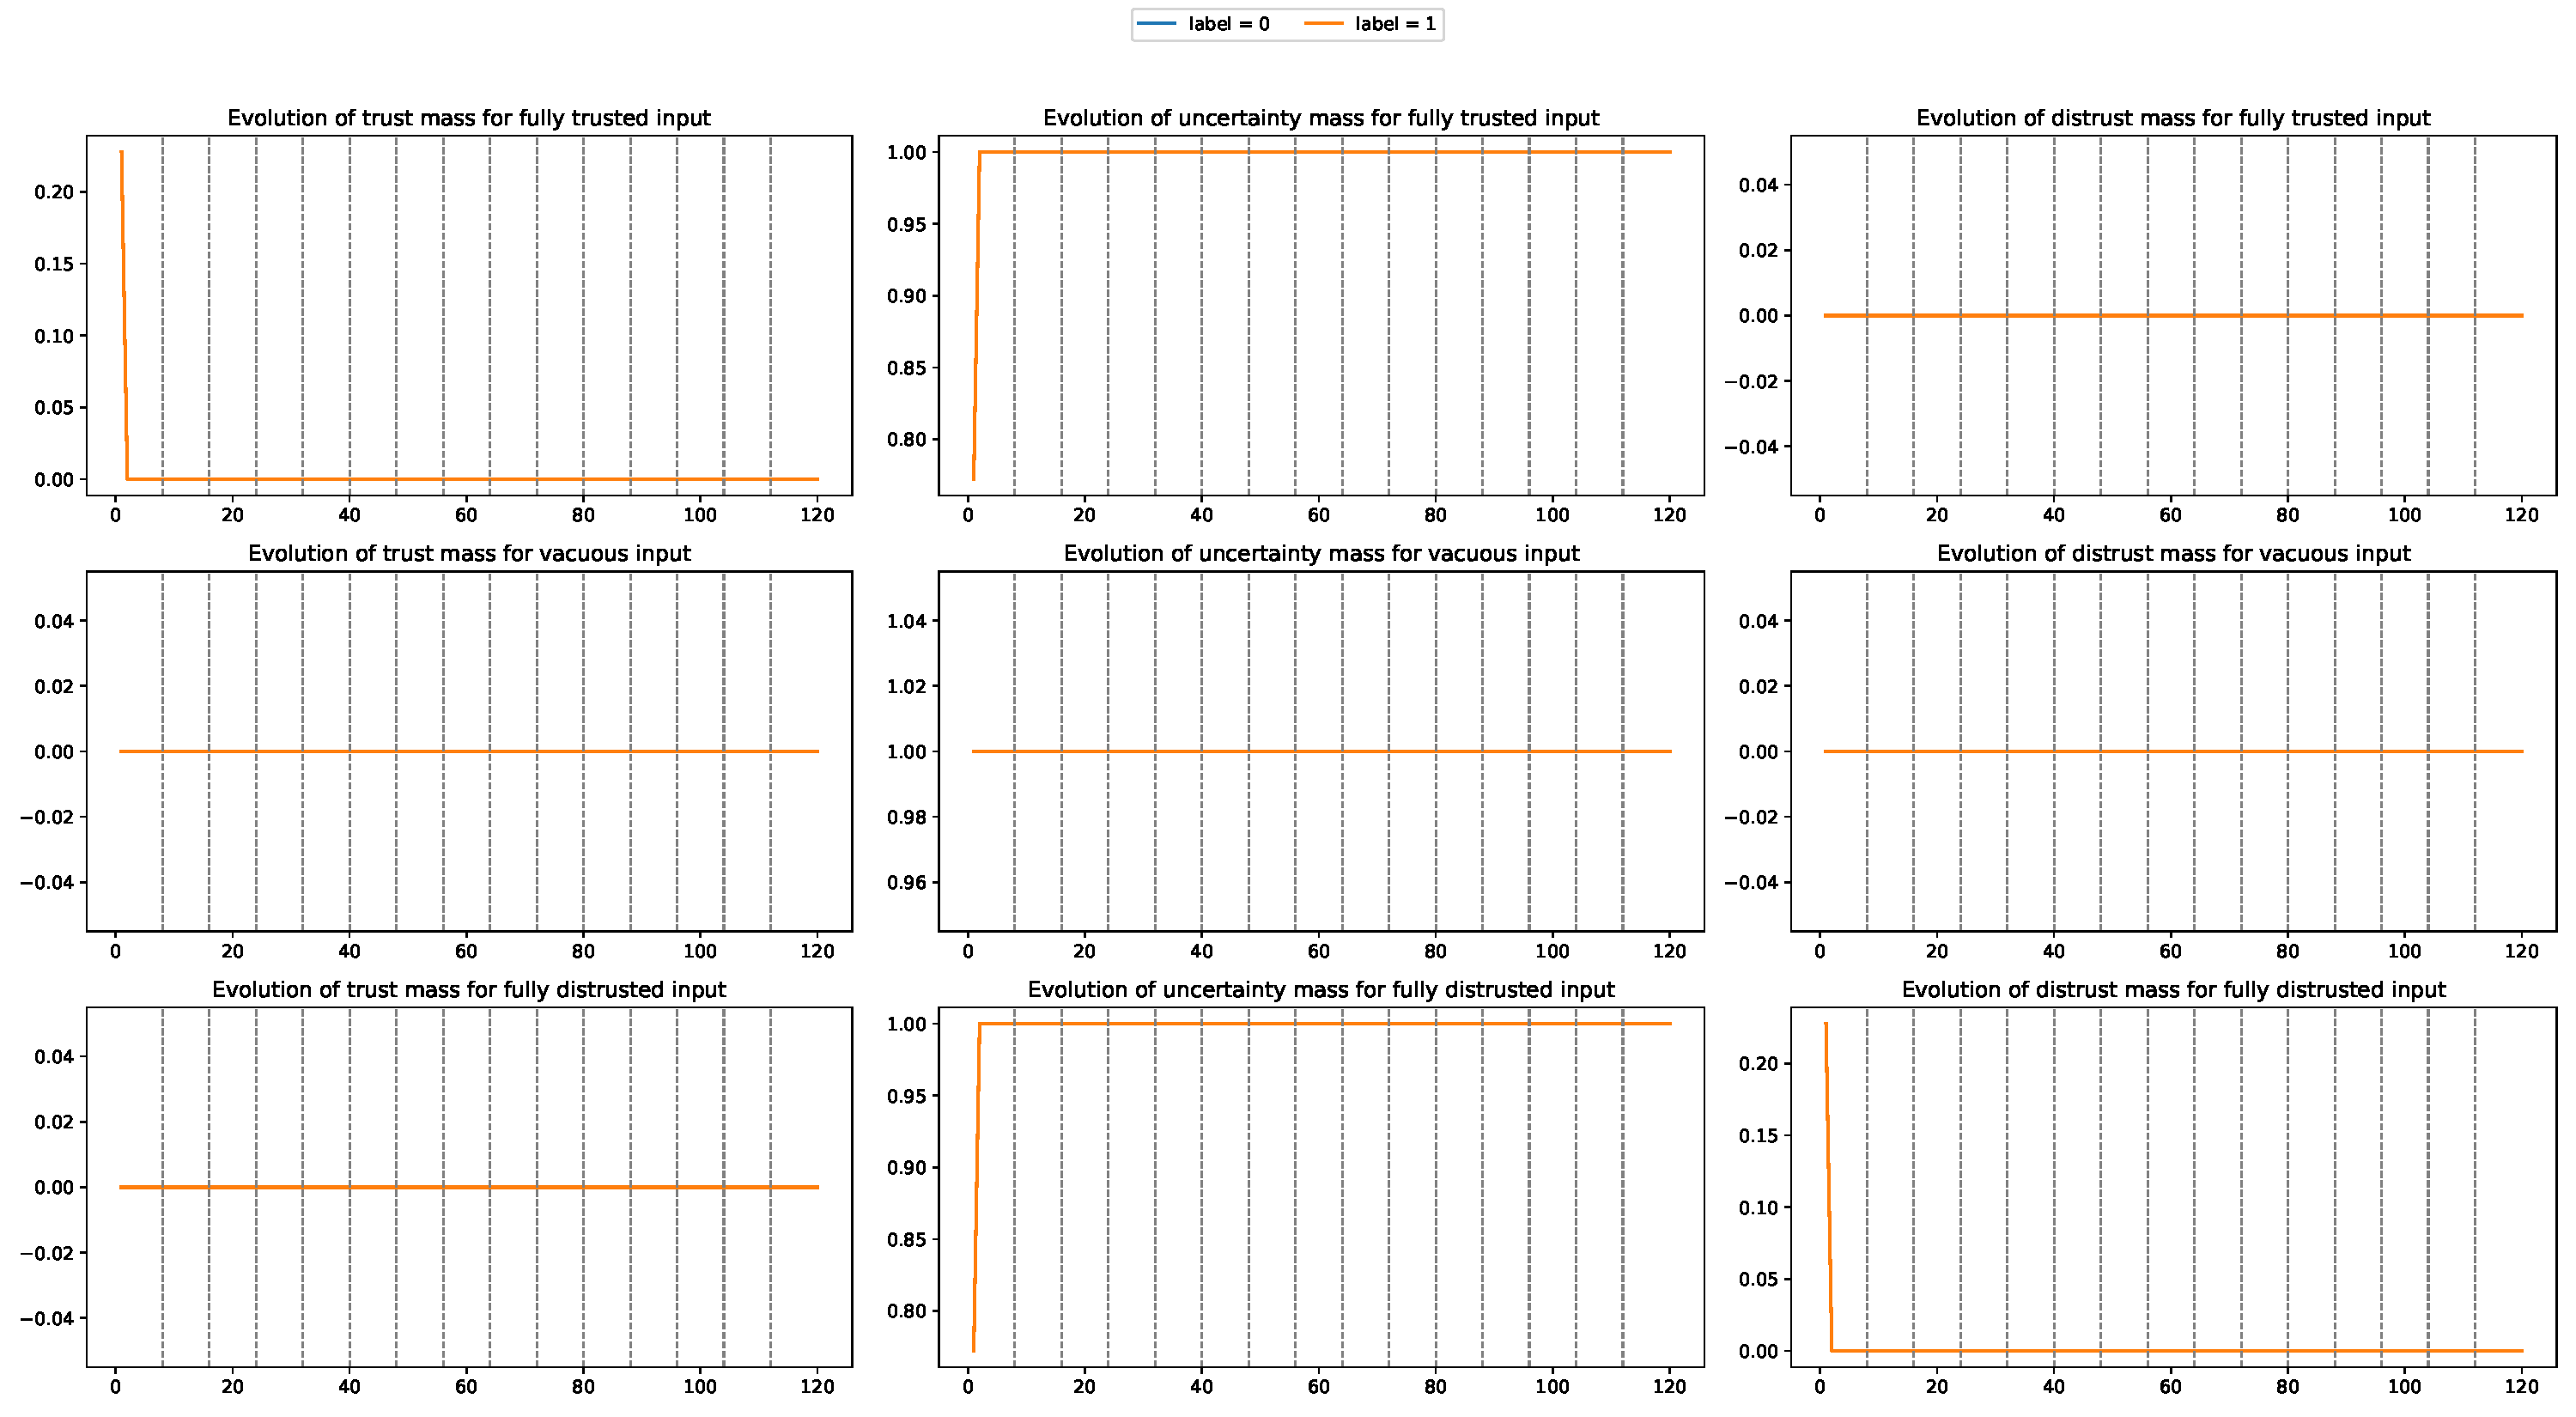
\includegraphics[width=0.8\textwidth]{latex/PTAS_Eval_cancer_16_distrust_vacuous_eps_0.1_PathSize_None__plot_ptas.pdf}
\caption{cancer\_16\_distrust\_vacuous, $\varepsilon$=0.1}
\end{figure}

\begin{figure}[htbp]
\centering
  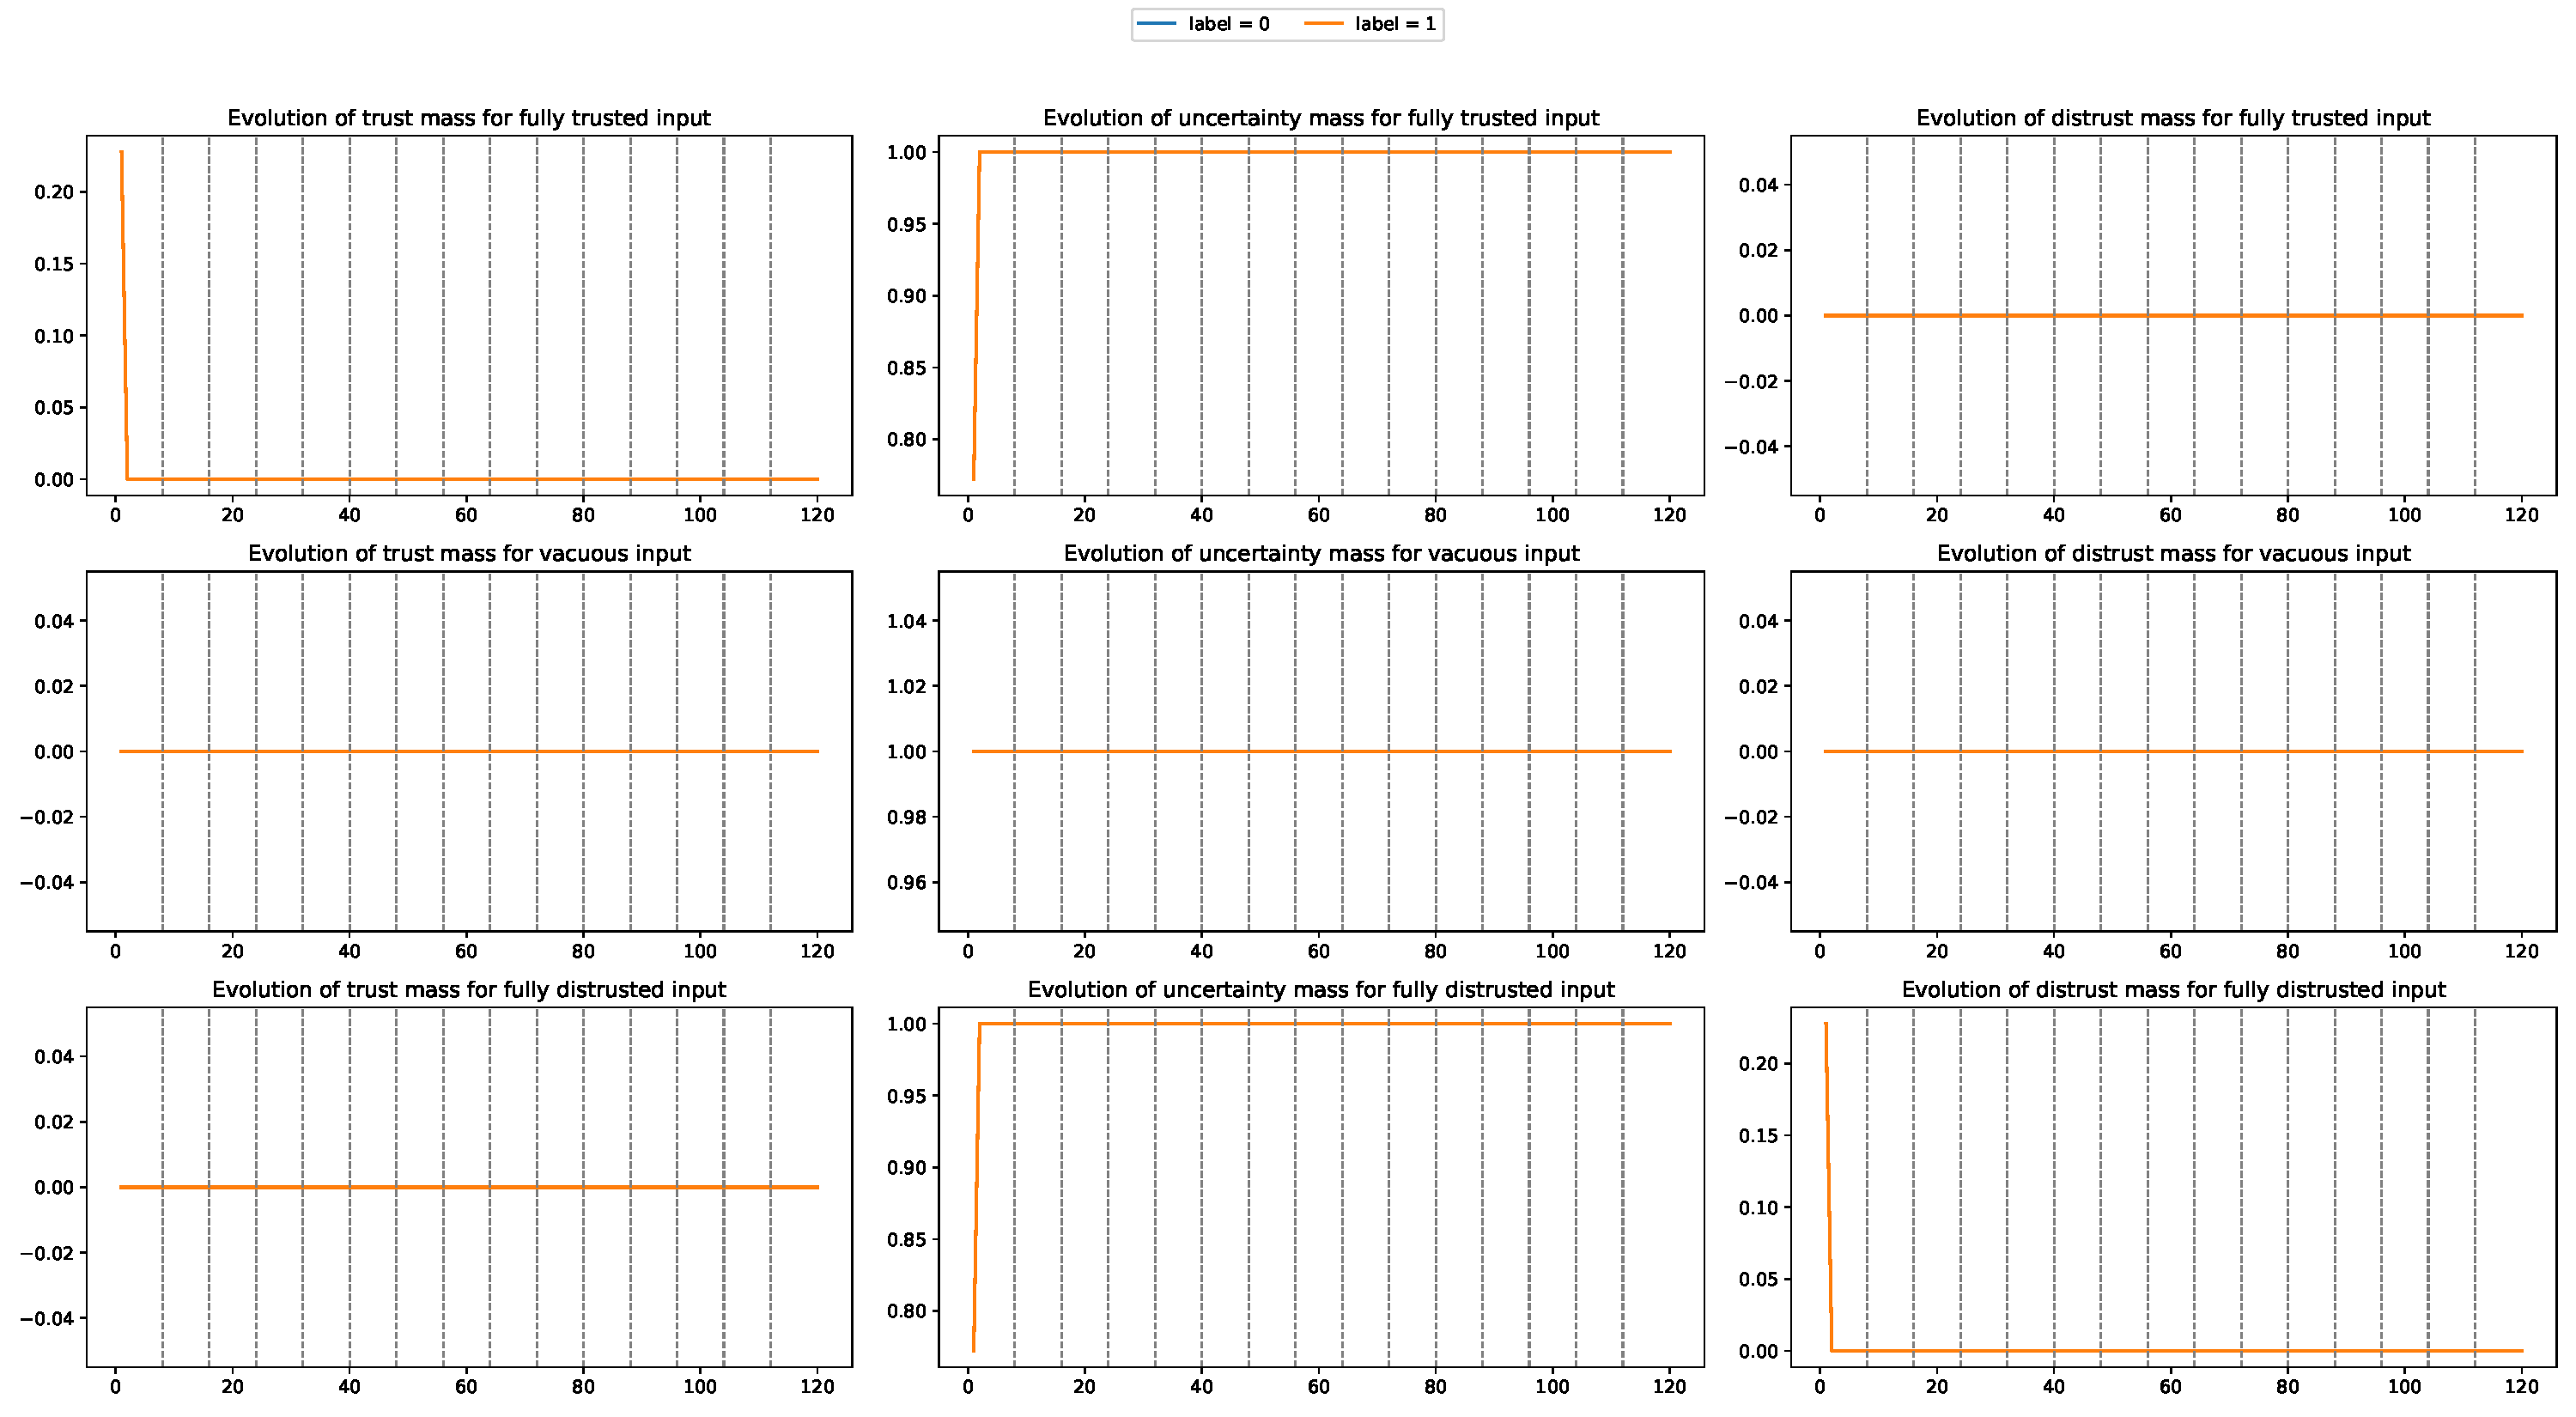
\includegraphics[width=0.8\textwidth]{latex/PTAS_Eval_cancer_16_distrust_vacuous_eps_1_PathSize_None__plot_ptas.pdf}
\caption{cancer\_16\_distrust\_vacuous, $\varepsilon$=1}
\end{figure}

\subsubsection{trust -- distrust}

\begin{figure}[htbp]
\centering
  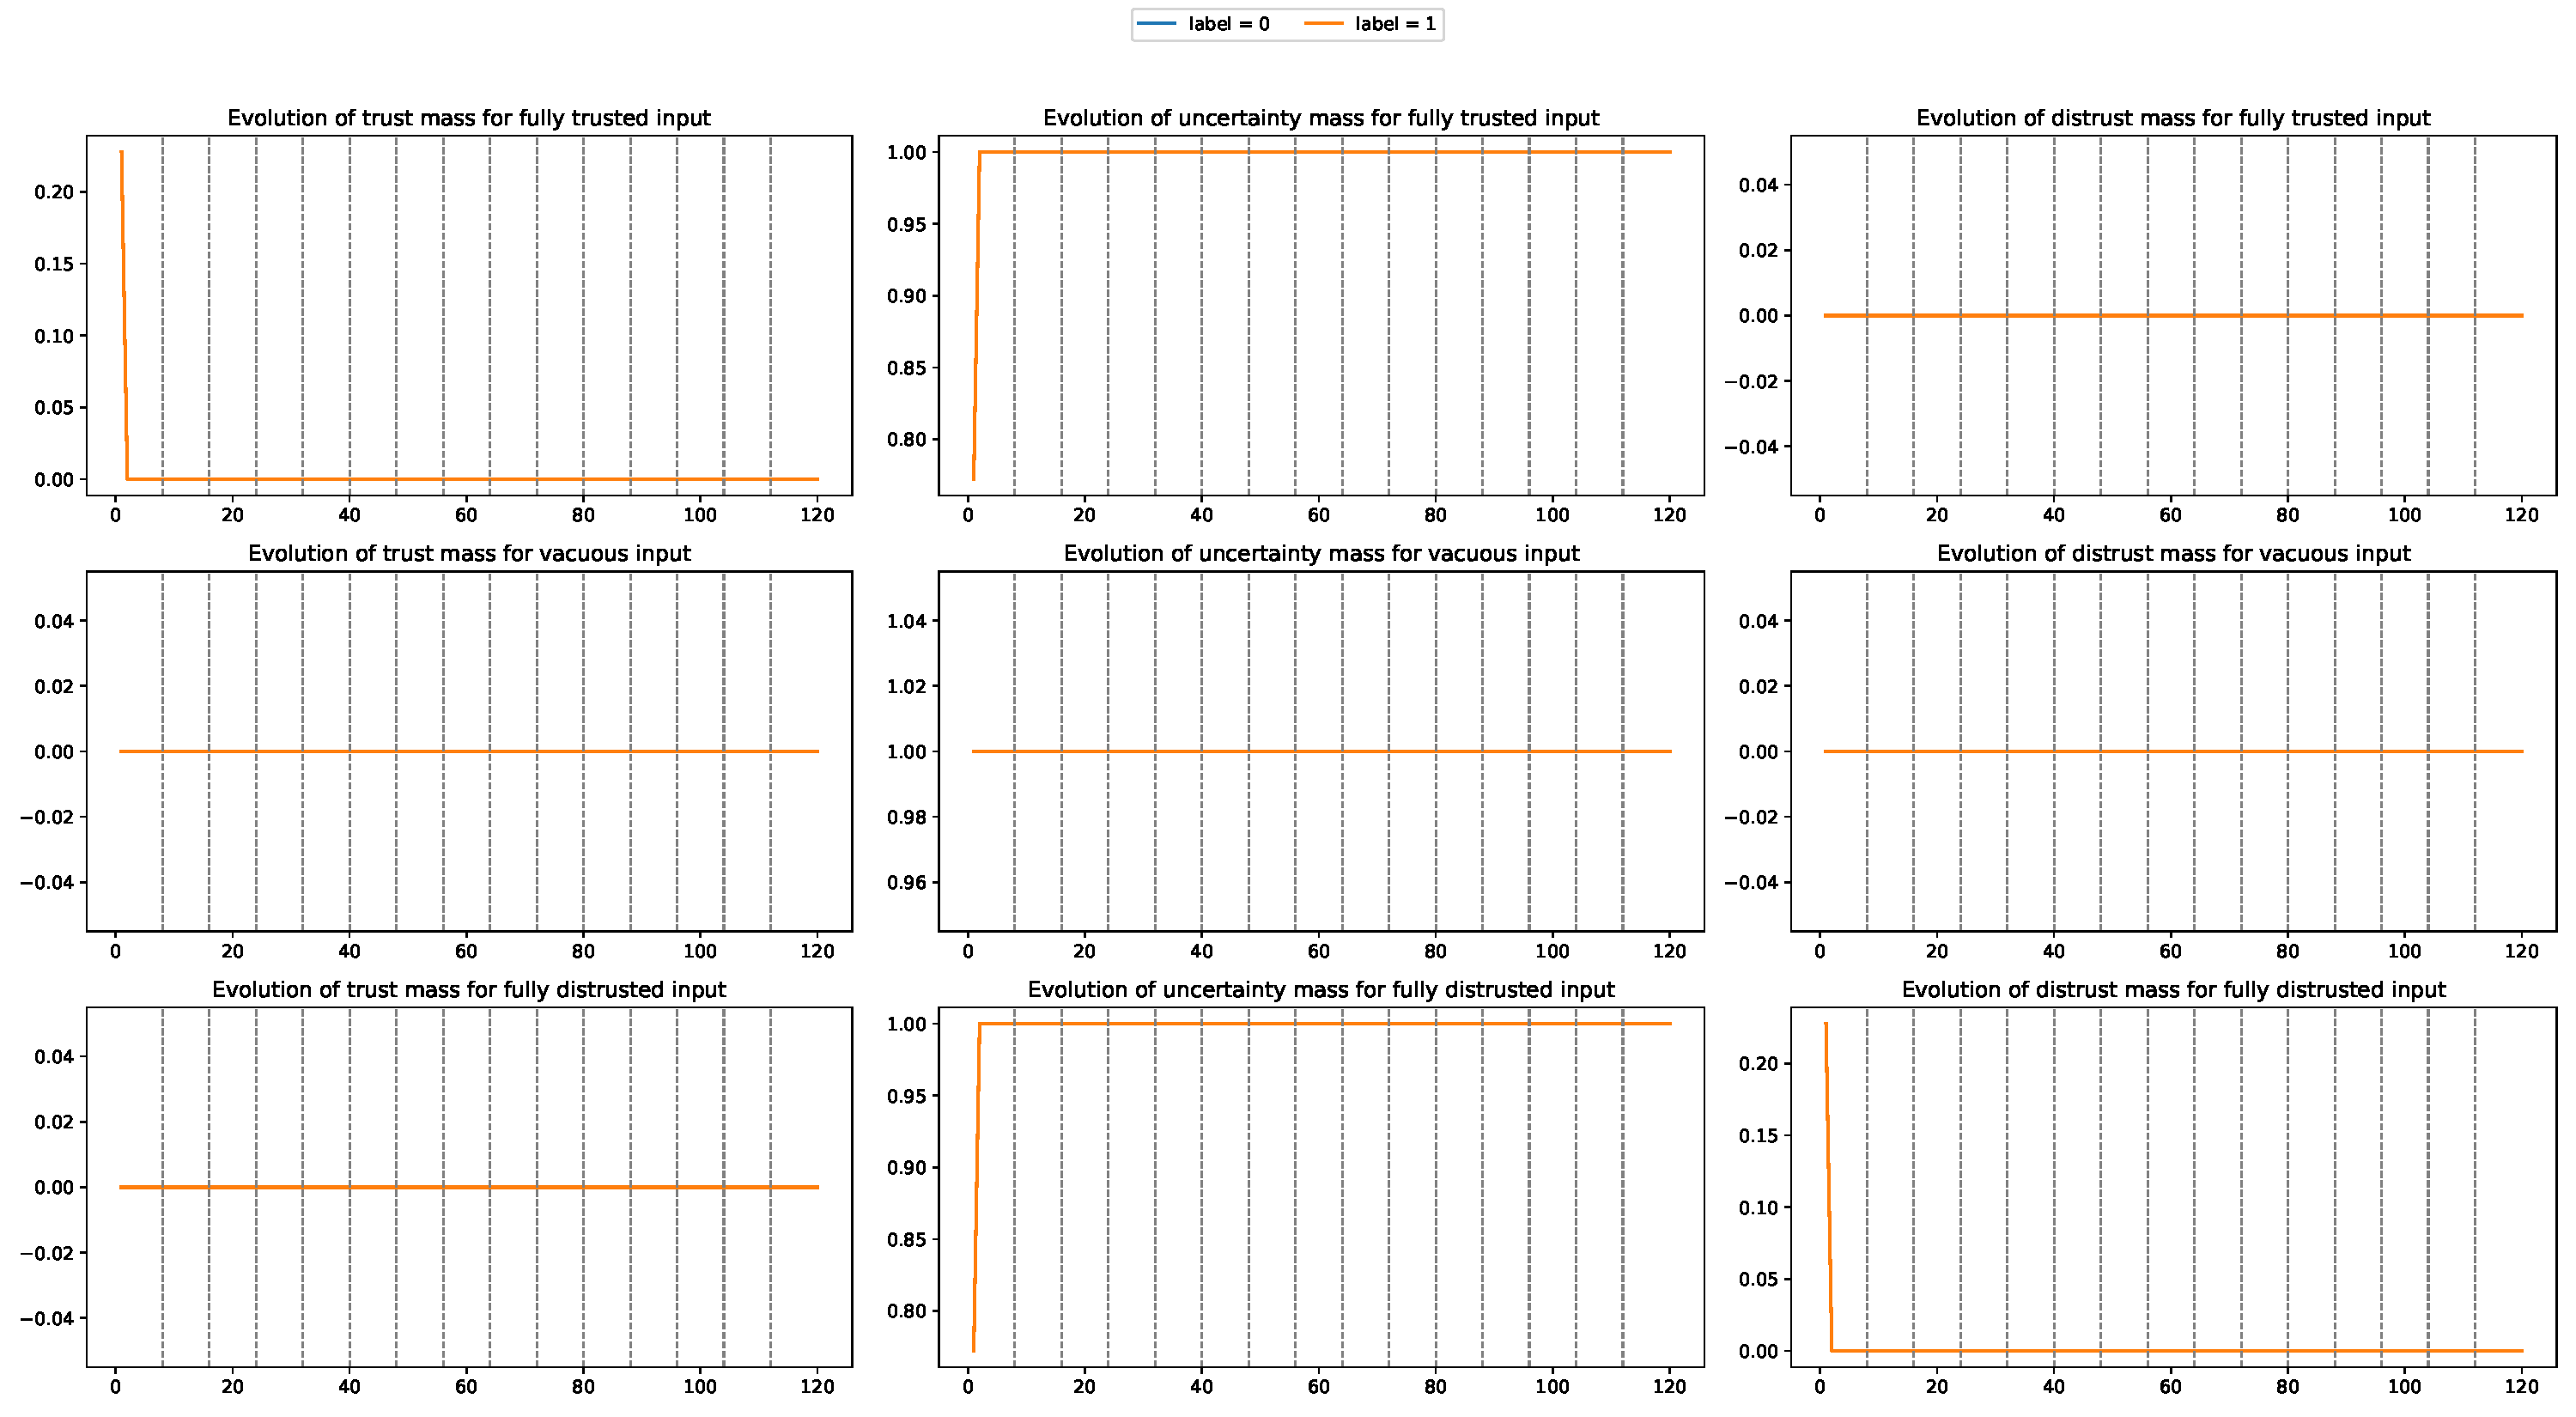
\includegraphics[width=0.8\textwidth]{latex/PTAS_Eval_cancer_16_trust_distrust_eps_0.001_PathSize_None__plot_ptas.pdf}
\caption{cancer\_16\_trust\_distrust, $\varepsilon$=0.001}
\end{figure}

\begin{figure}[htbp]
\centering
  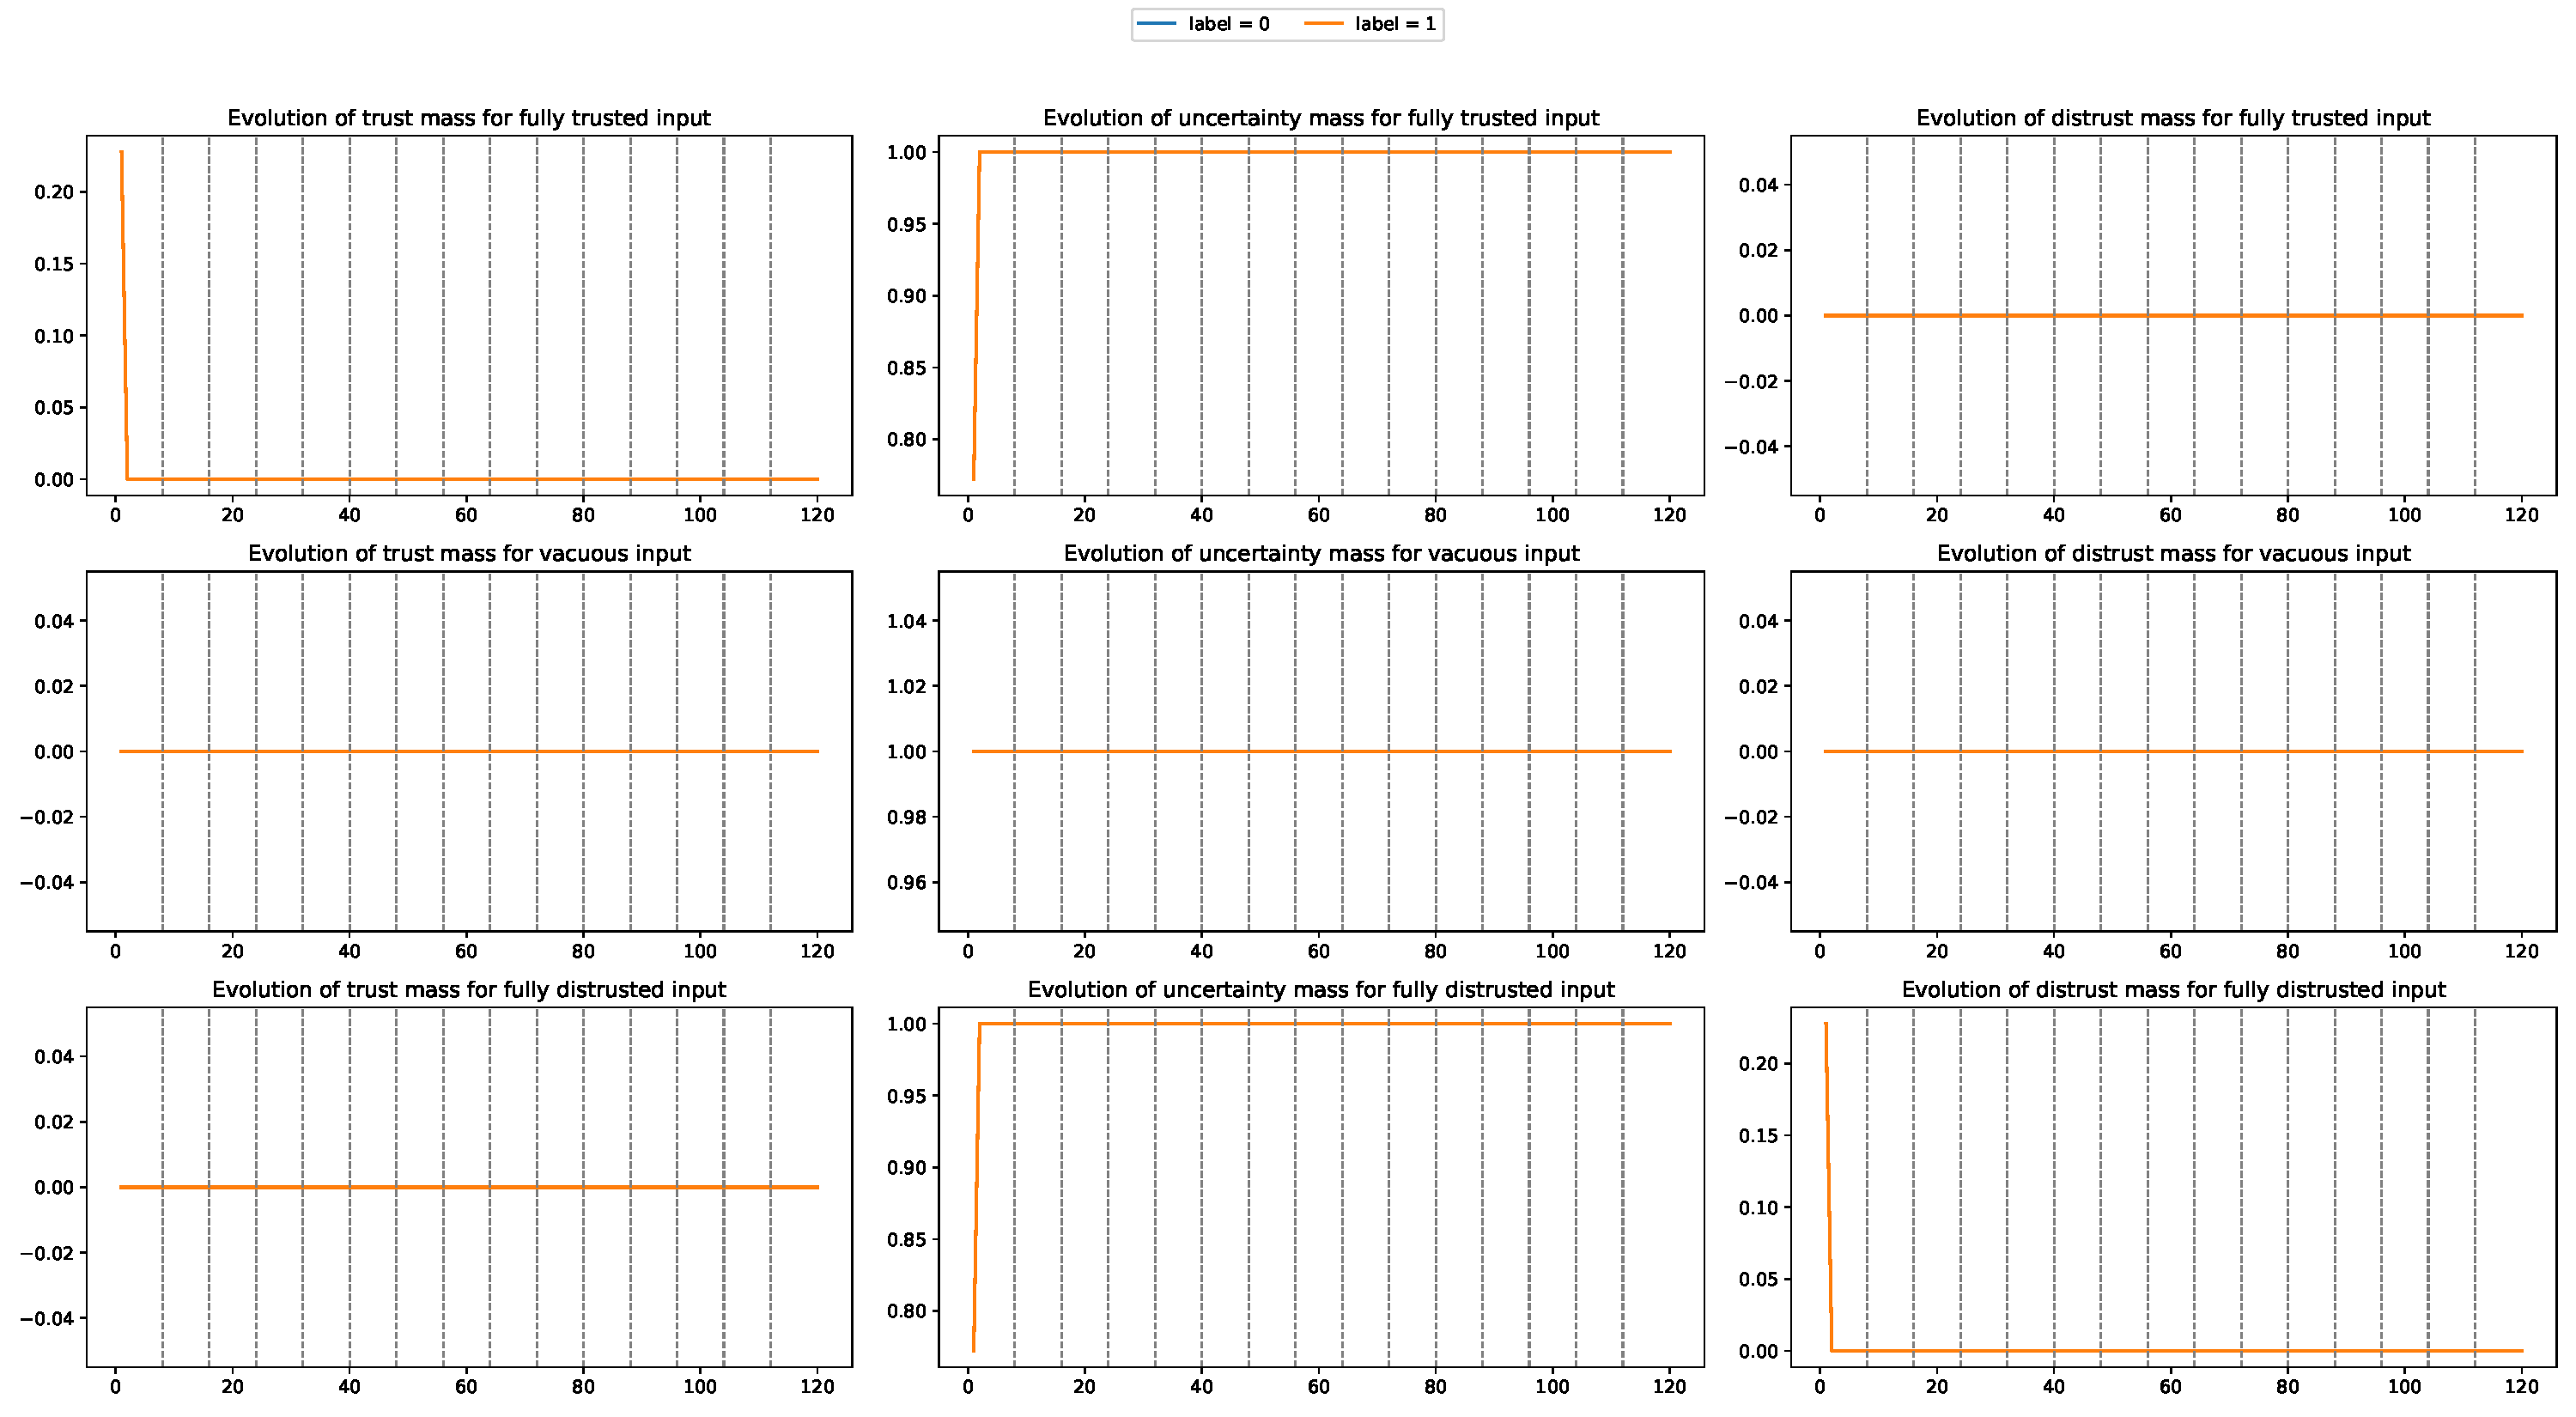
\includegraphics[width=0.8\textwidth]{latex/PTAS_Eval_cancer_16_trust_distrust_eps_0.01_PathSize_None__plot_ptas.pdf}
\caption{cancer\_16\_trust\_distrust, $\varepsilon$=0.01}
\end{figure}

\begin{figure}[htbp]
\centering
  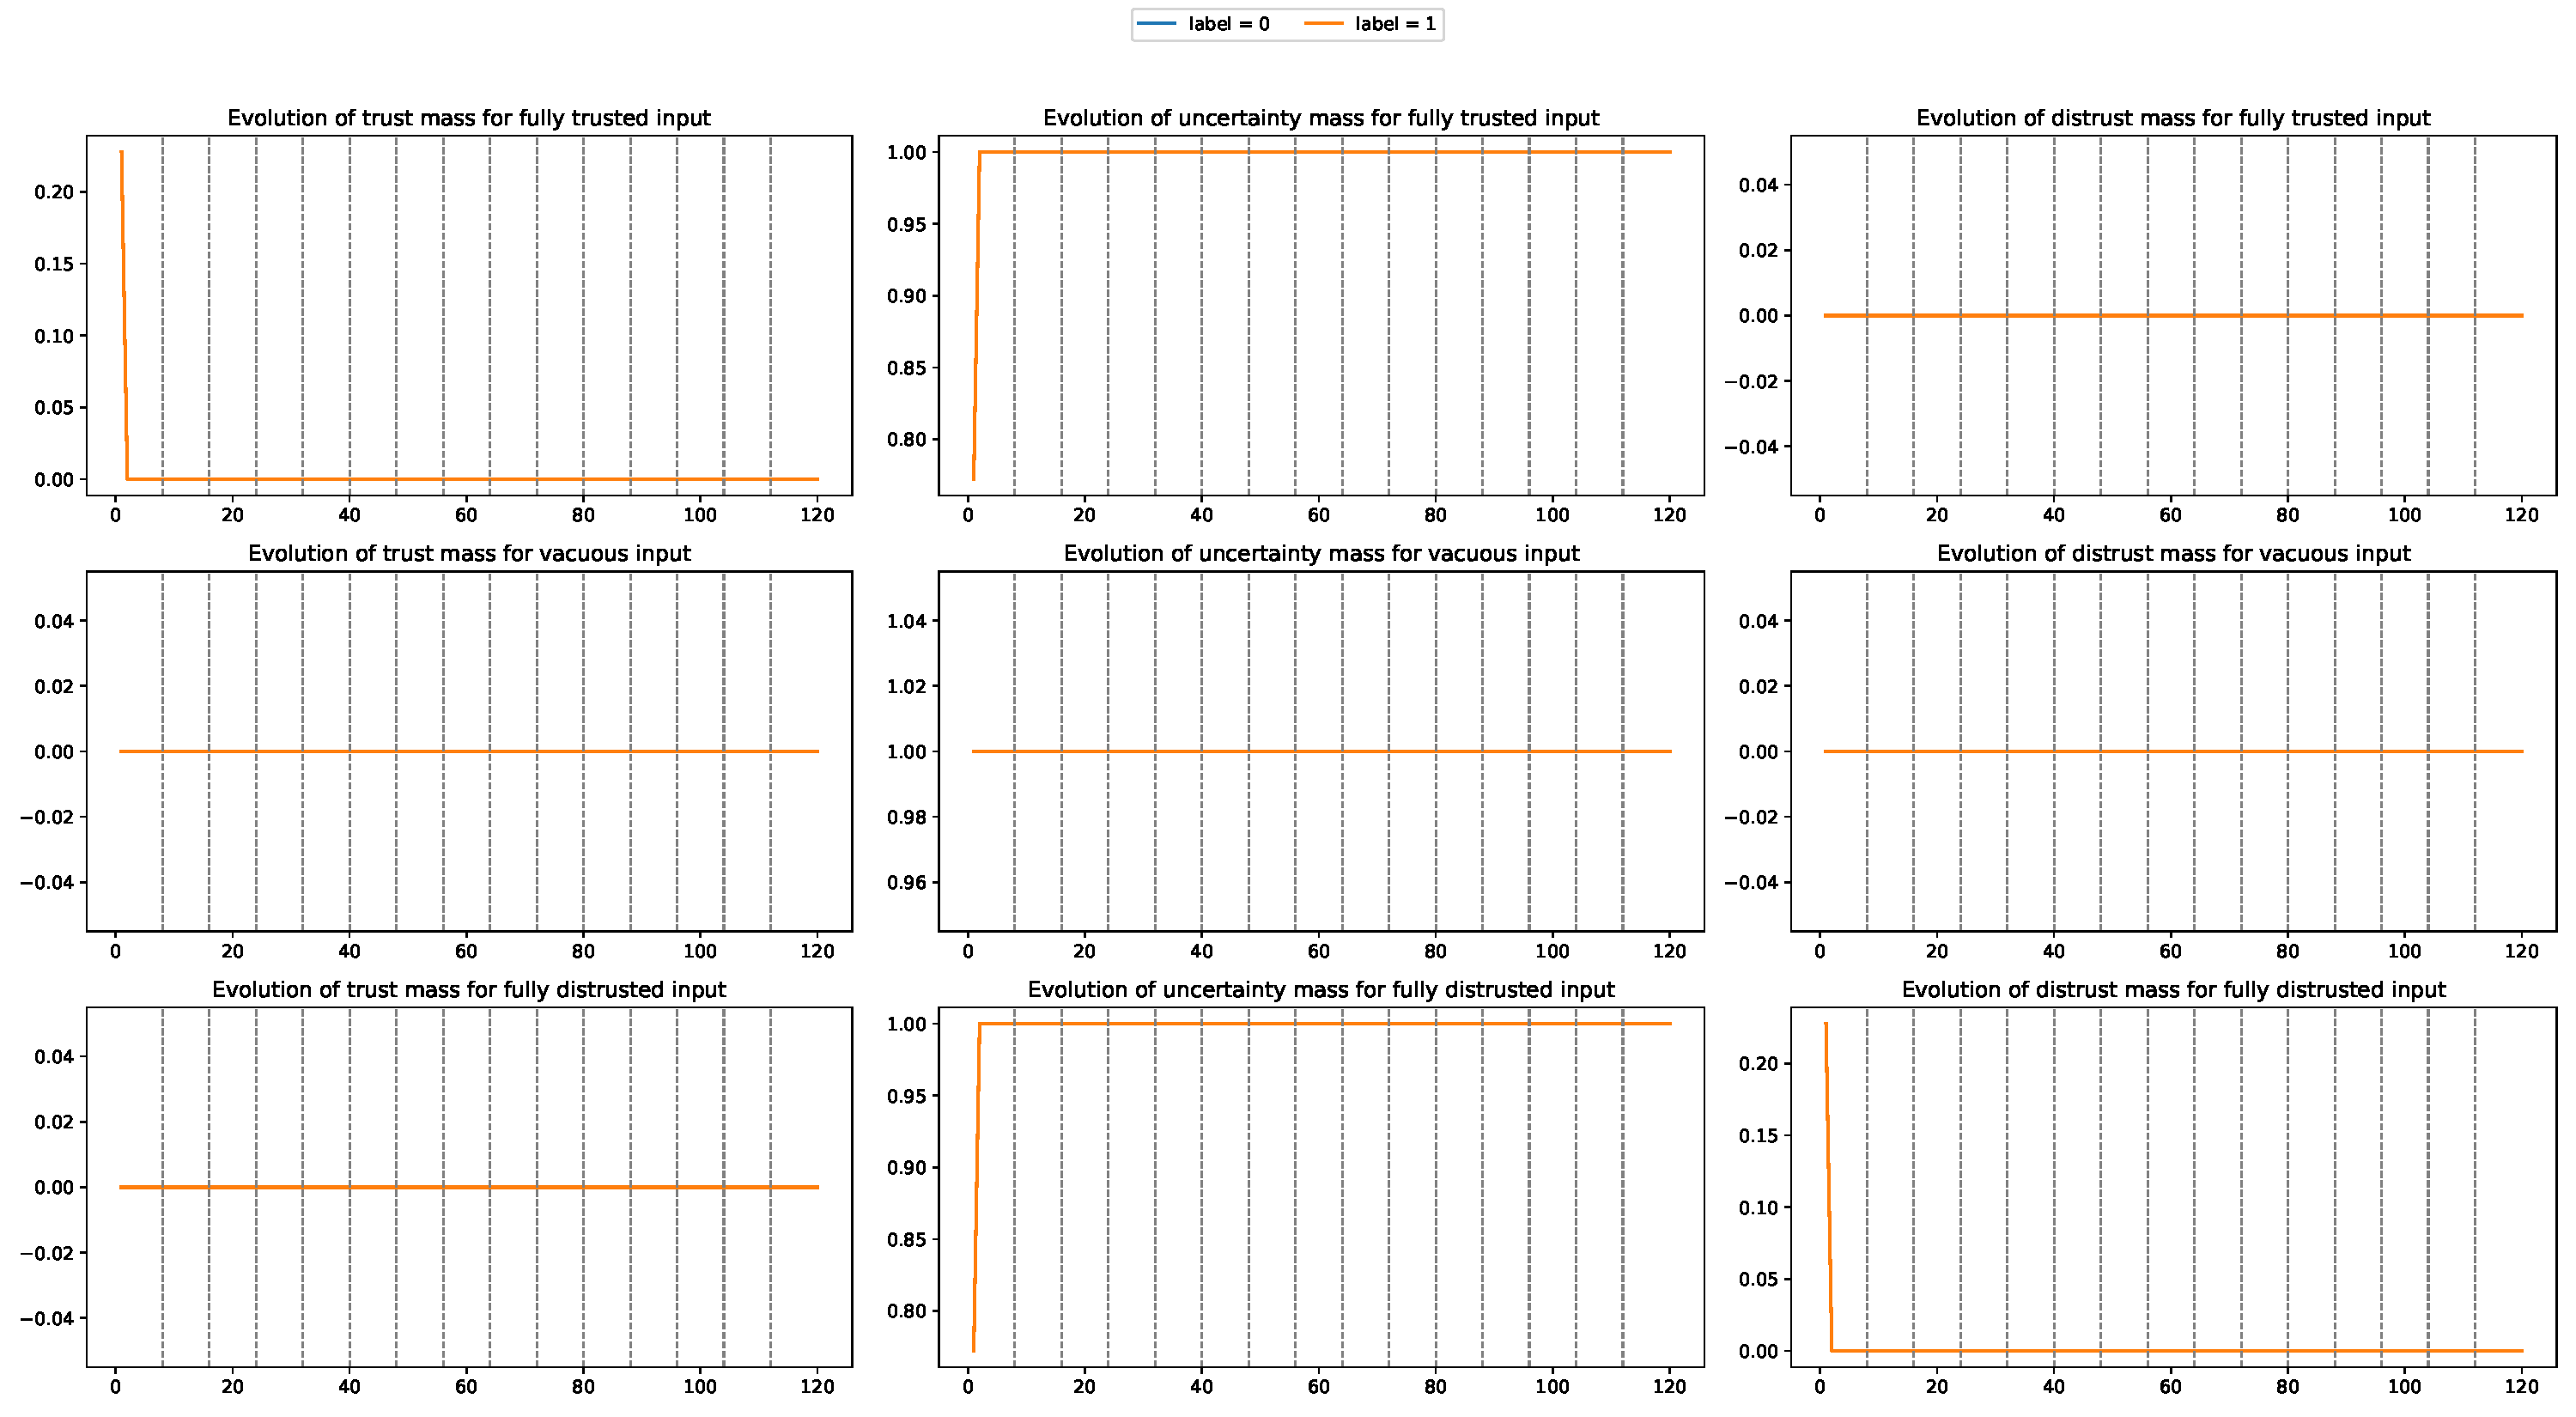
\includegraphics[width=0.8\textwidth]{latex/PTAS_Eval_cancer_16_trust_distrust_eps_0.1_PathSize_None__plot_ptas.pdf}
\caption{cancer\_16\_trust\_distrust, $\varepsilon$=0.1}
\end{figure}

\begin{figure}[htbp]
\centering
  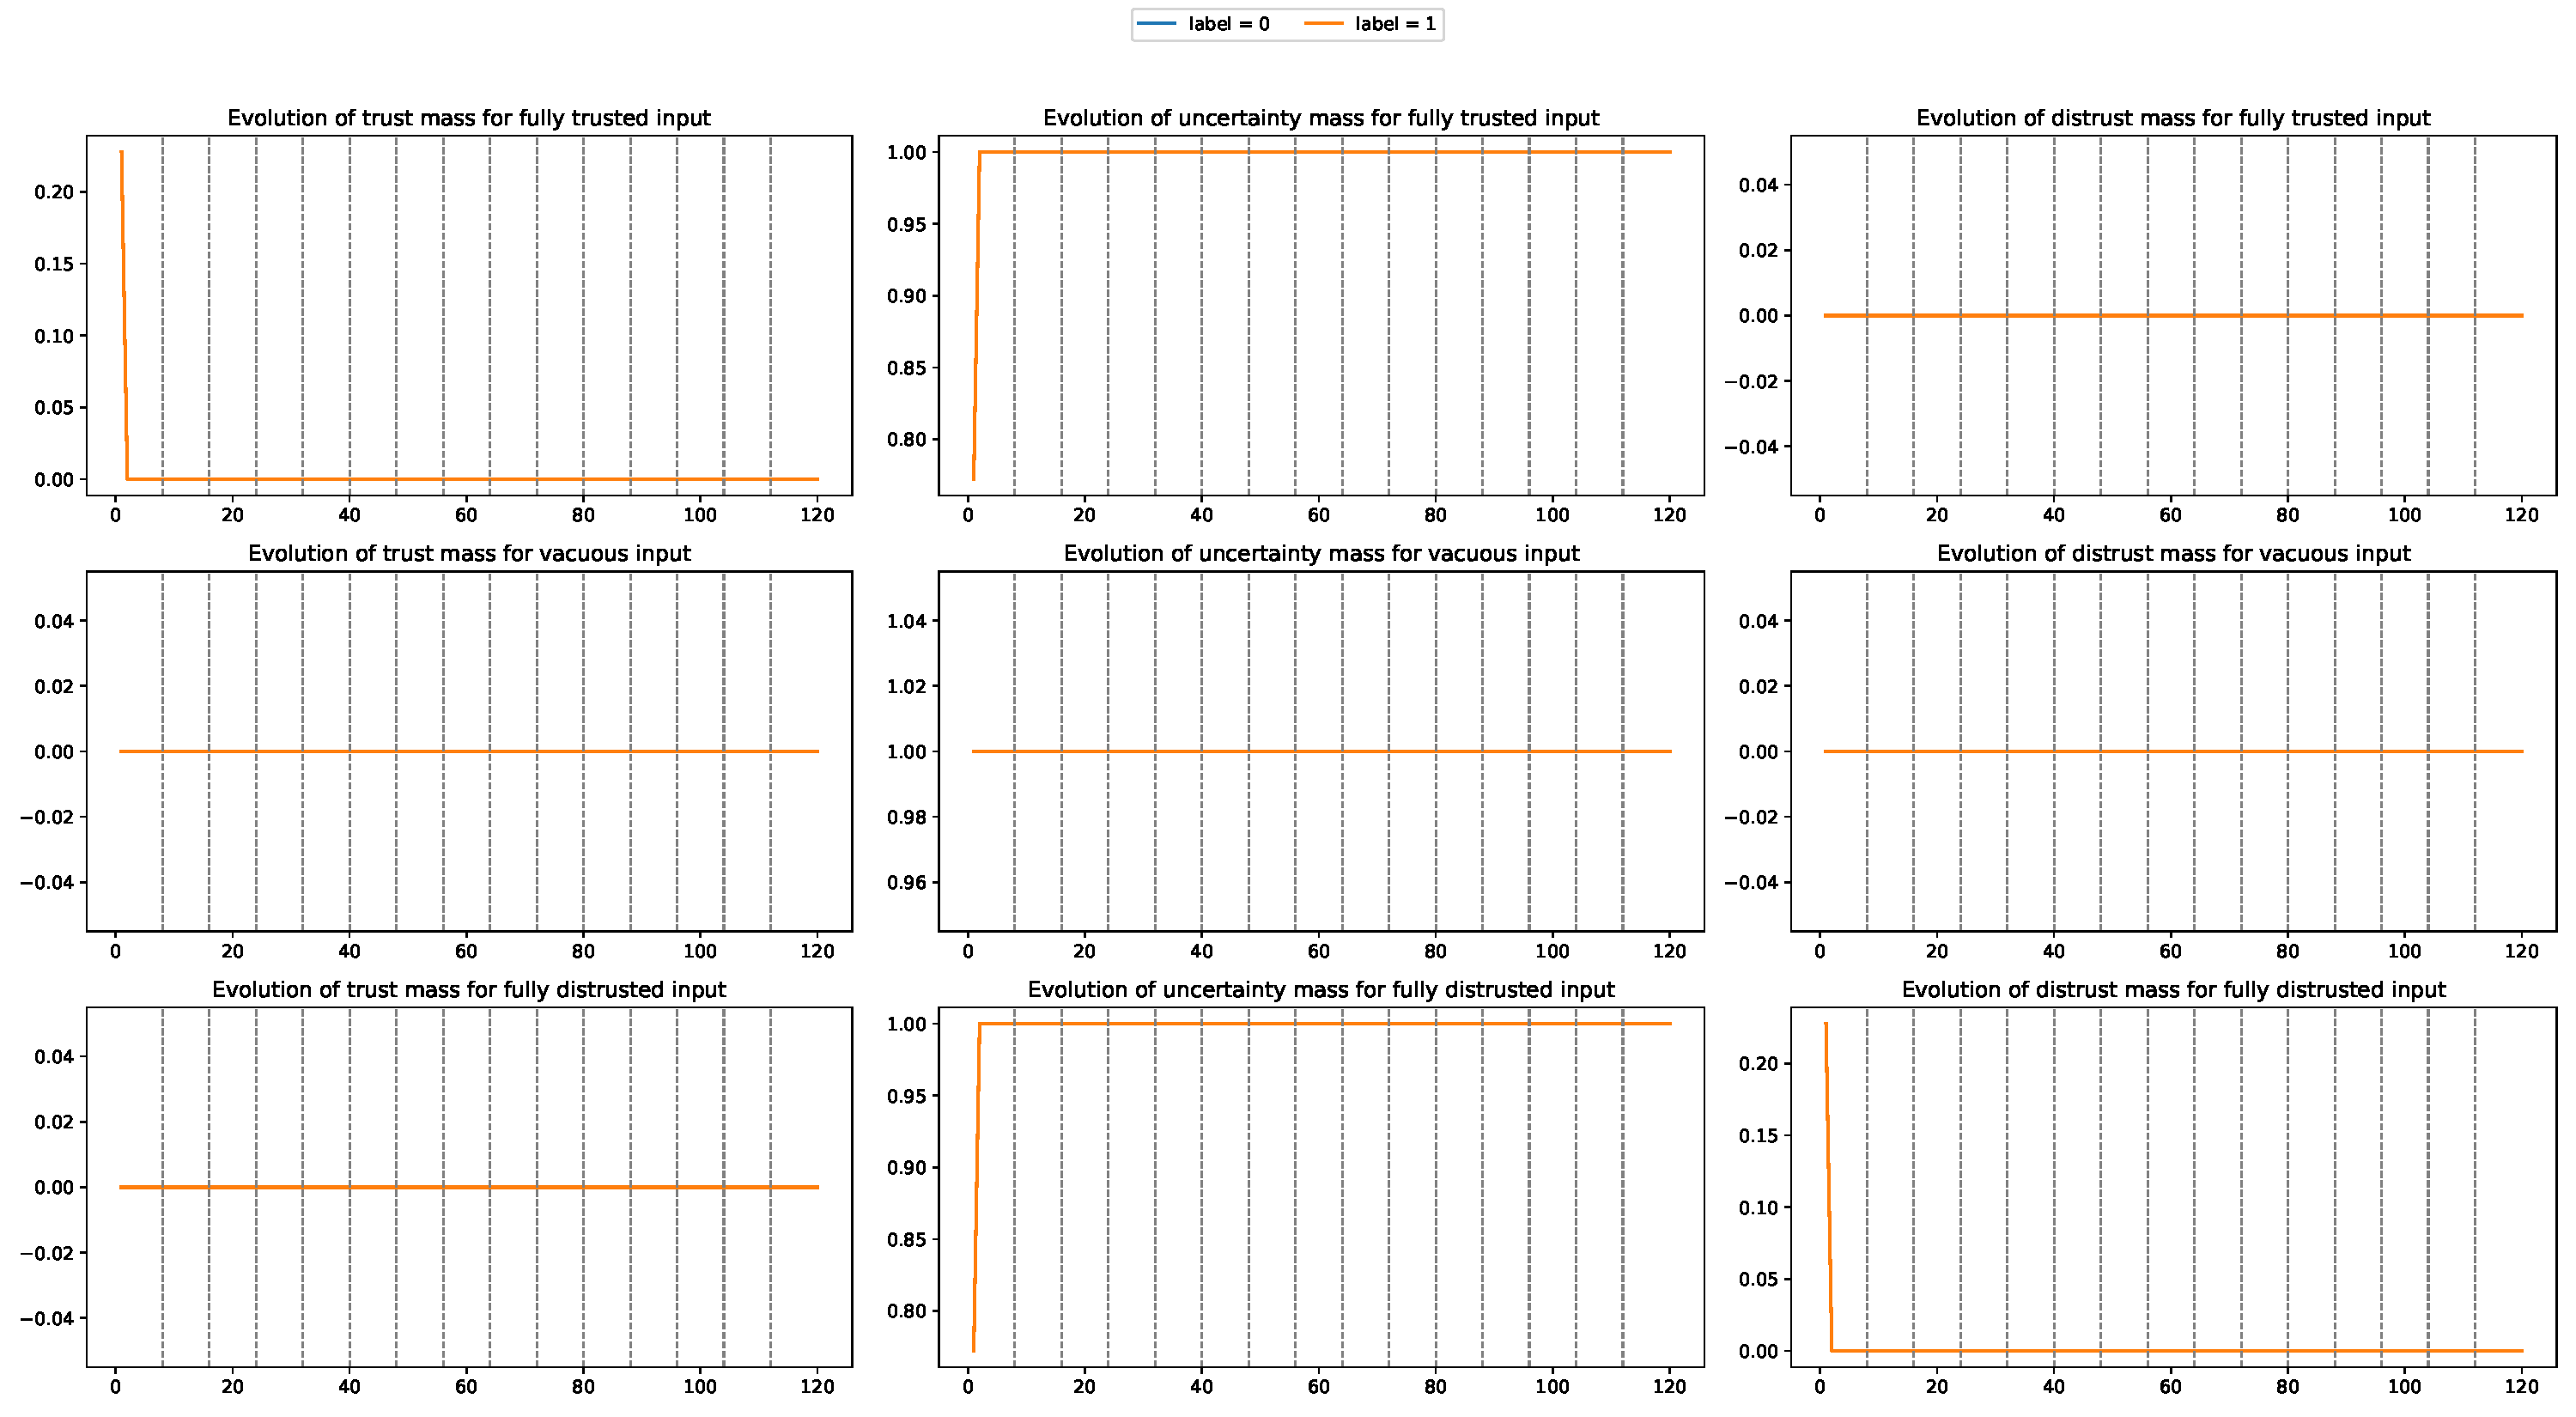
\includegraphics[width=0.8\textwidth]{latex/PTAS_Eval_cancer_16_trust_distrust_eps_1_PathSize_None__plot_ptas.pdf}
\caption{cancer\_16\_trust\_distrust, $\varepsilon$=1}
\end{figure}

\subsubsection{trust -- trust}

\begin{figure}[htbp]
\centering
  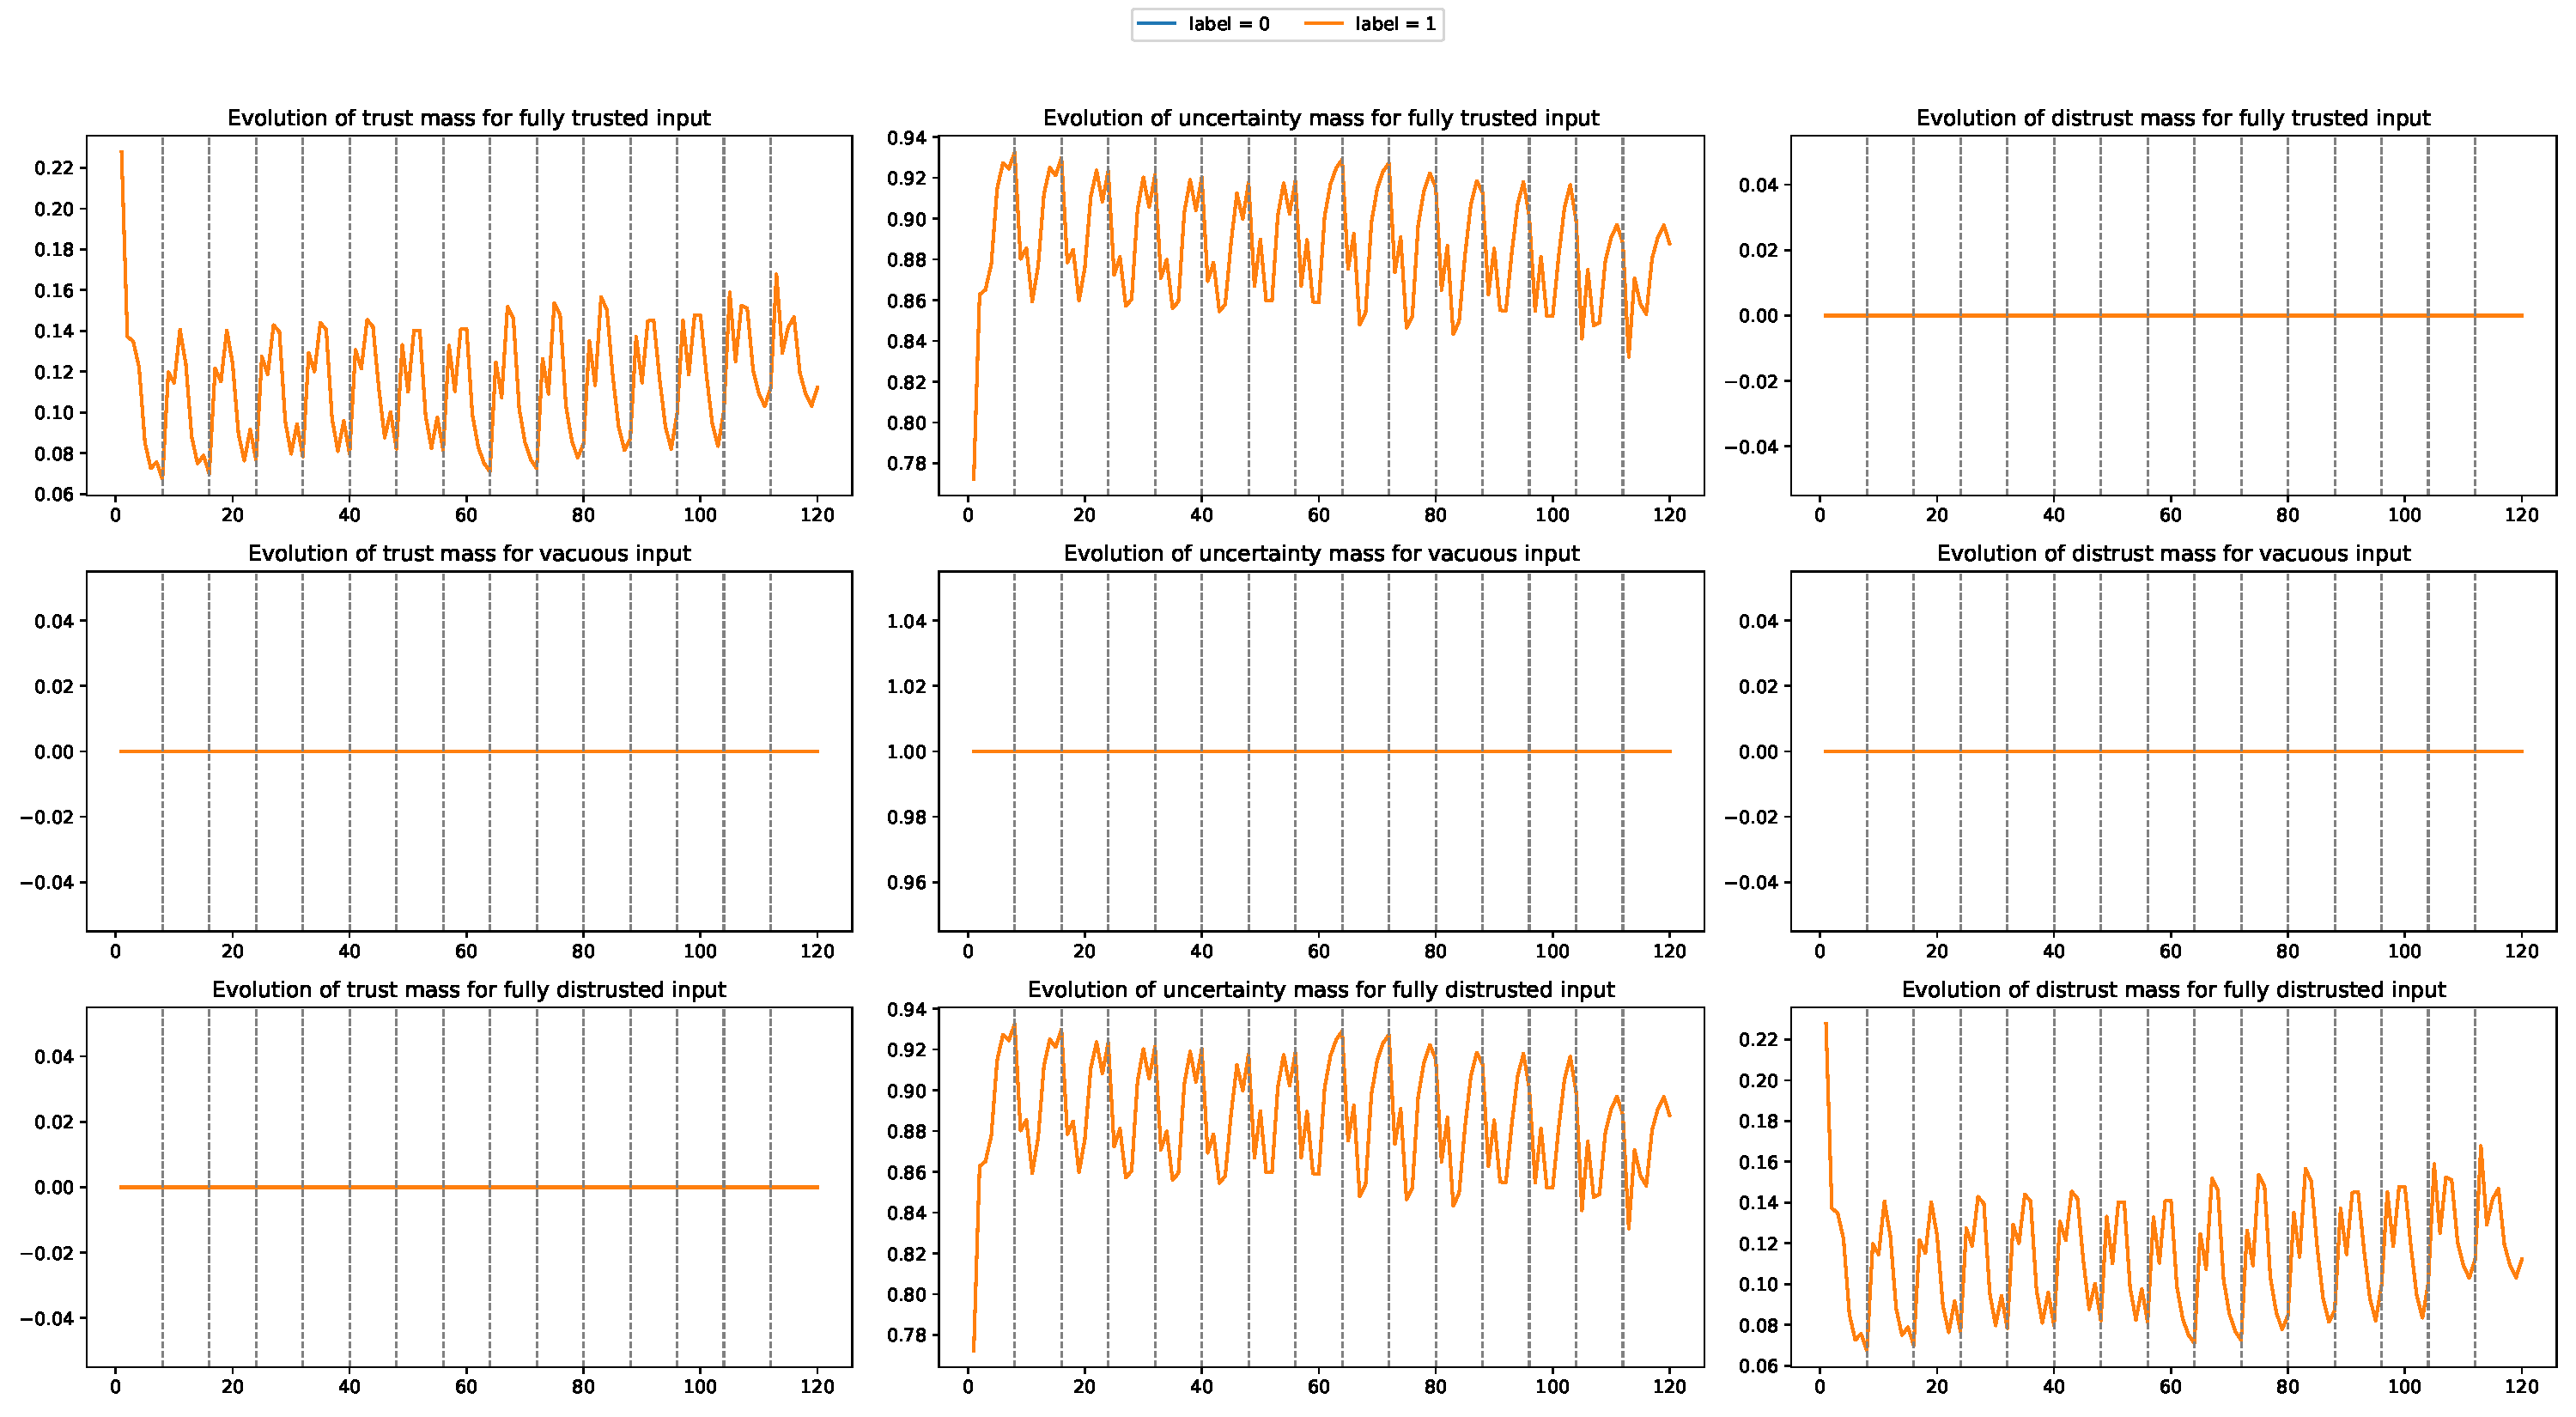
\includegraphics[width=0.8\textwidth]{latex/PTAS_Eval_cancer_16_trust_trust_eps_0.001_PathSize_None__plot_ptas.pdf}
\caption{cancer\_16\_trust\_trust, $\varepsilon$=0.001}
\end{figure}

\begin{figure}[htbp]
\centering
  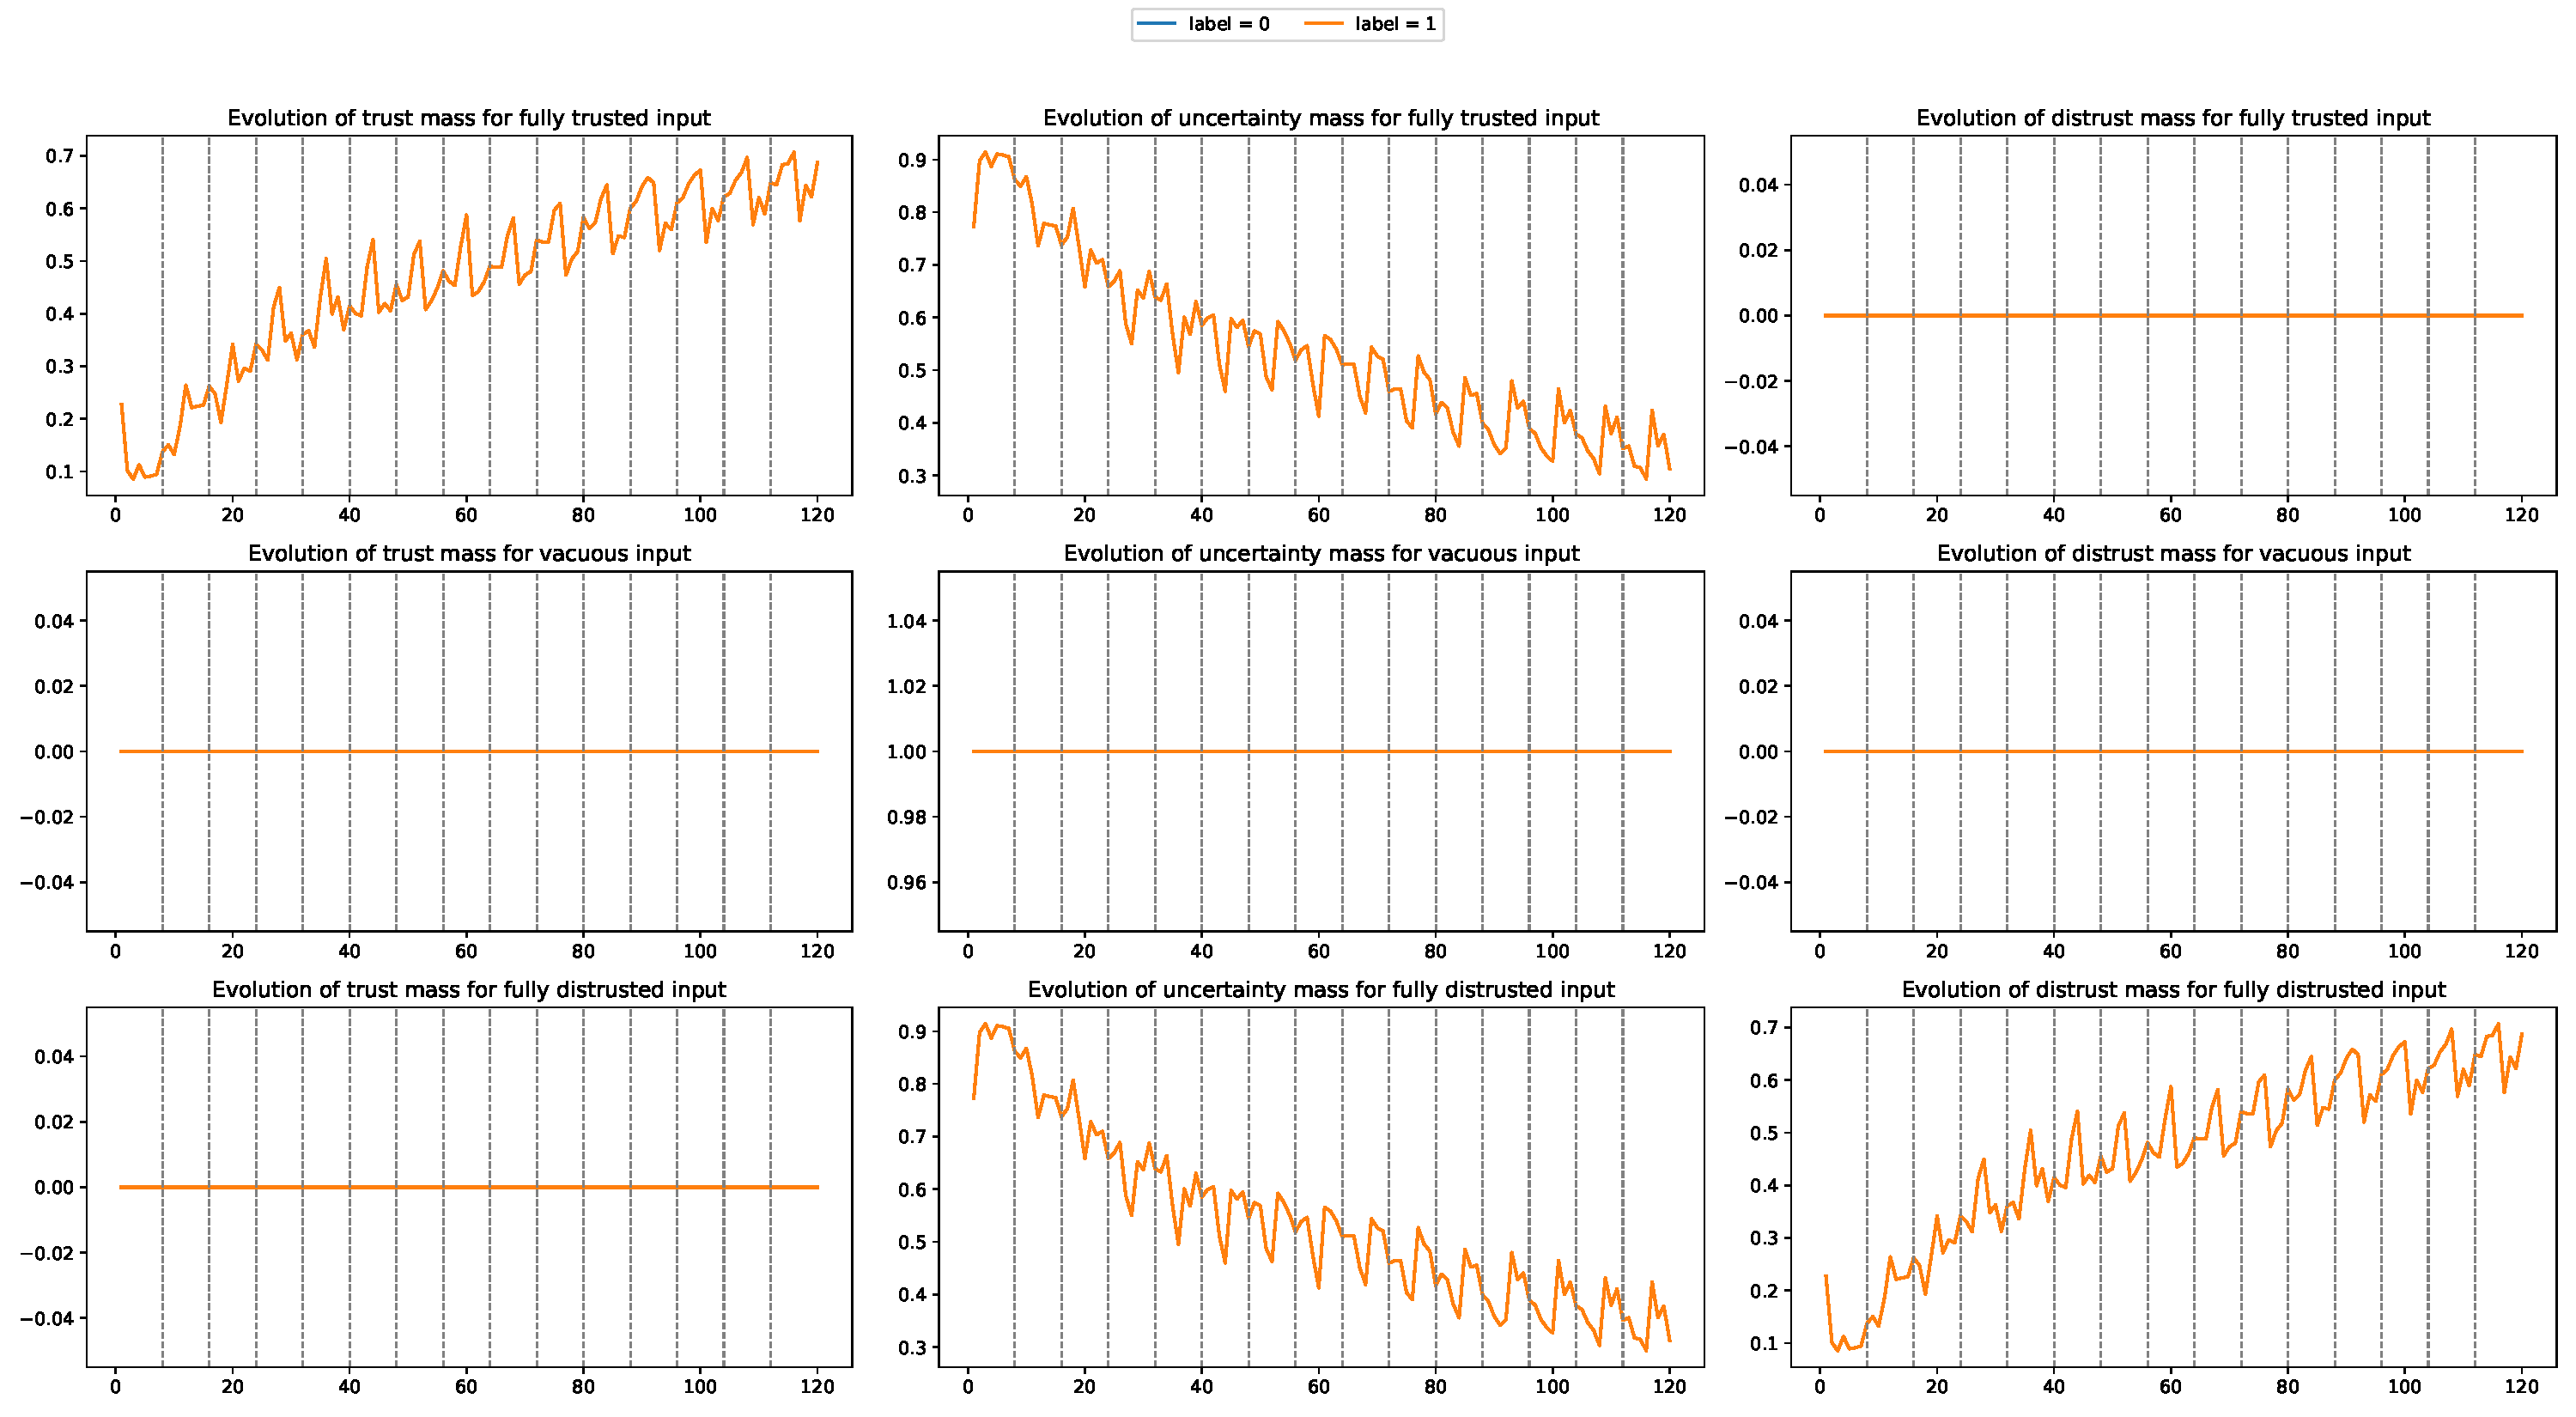
\includegraphics[width=0.8\textwidth]{latex/PTAS_Eval_cancer_16_trust_trust_eps_0.01_PathSize_None__plot_ptas.pdf}
\caption{cancer\_16\_trust\_trust, $\varepsilon$=0.01}
\end{figure}

\begin{figure}[htbp]
\centering
  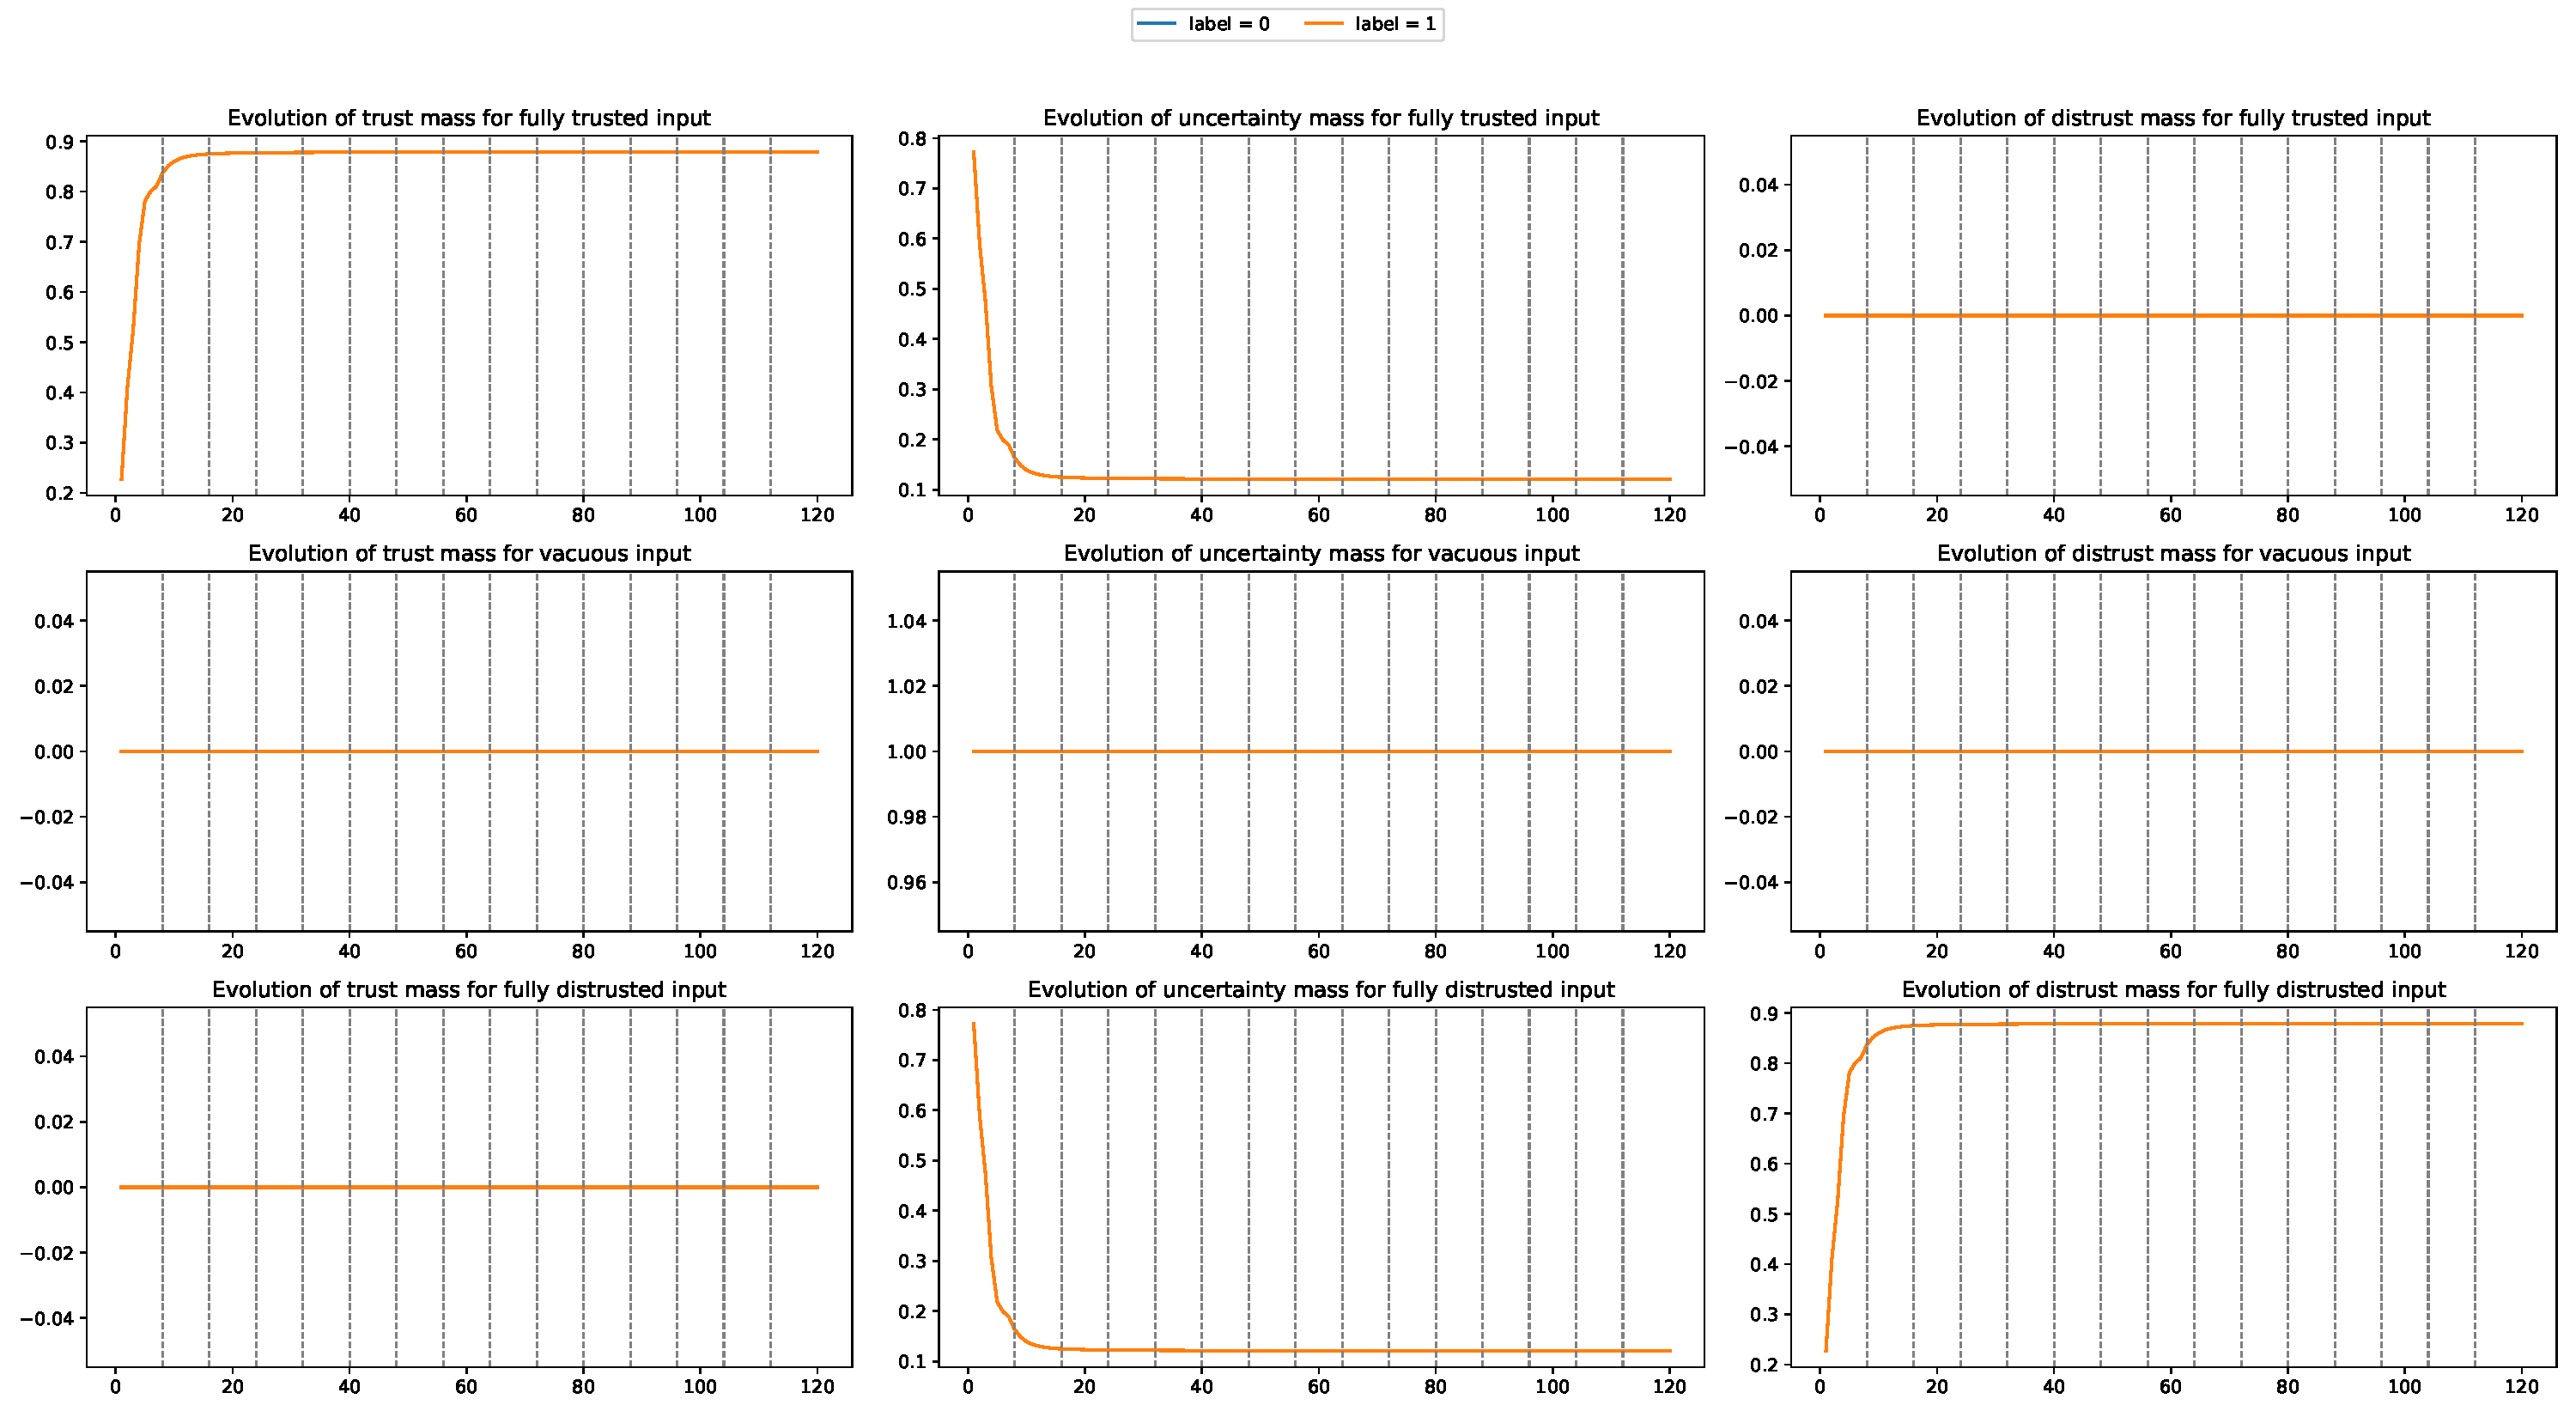
\includegraphics[width=0.8\textwidth]{latex/PTAS_Eval_cancer_16_trust_trust_eps_0.1_PathSize_None__plot_ptas.pdf}
\caption{cancer\_16\_trust\_trust, $\varepsilon$=0.1}
\end{figure}

\begin{figure}[htbp]
\centering
  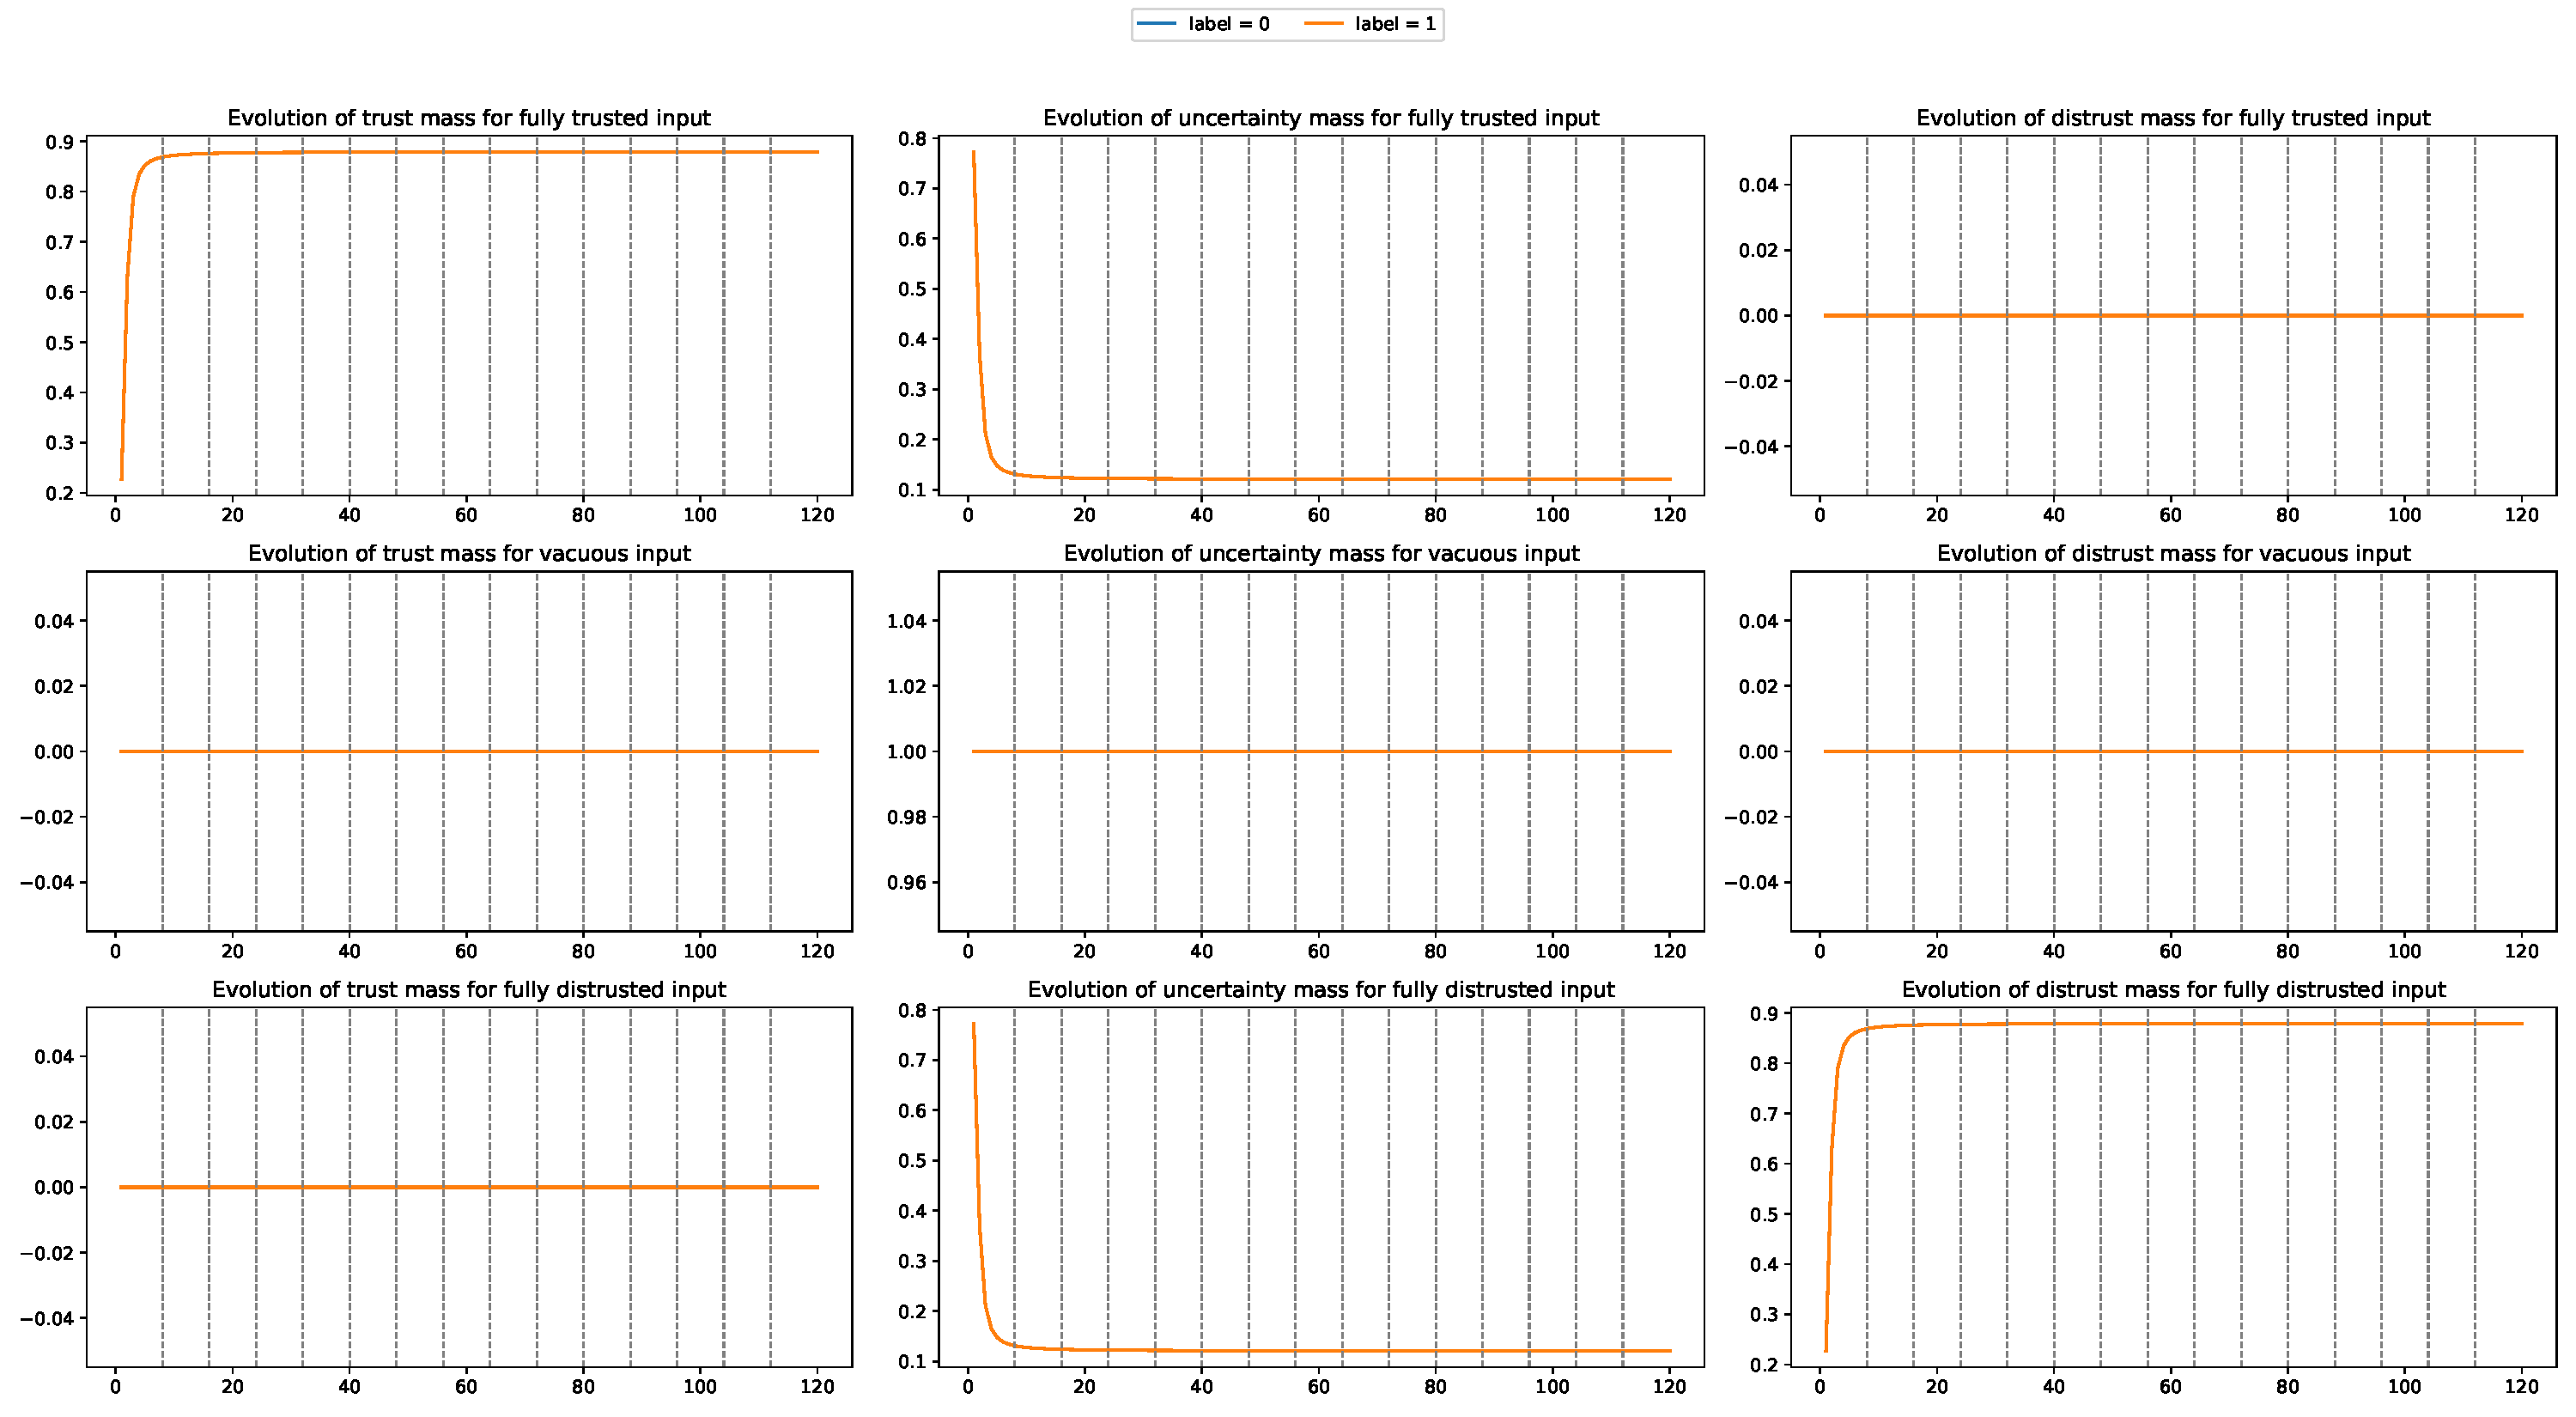
\includegraphics[width=0.8\textwidth]{latex/PTAS_Eval_cancer_16_trust_trust_eps_1_PathSize_None__plot_ptas.pdf}
\caption{cancer\_16\_trust\_trust, $\varepsilon$=1}
\end{figure}

\subsubsection{trust -- vacuous}

\begin{figure}[htbp]
\centering
  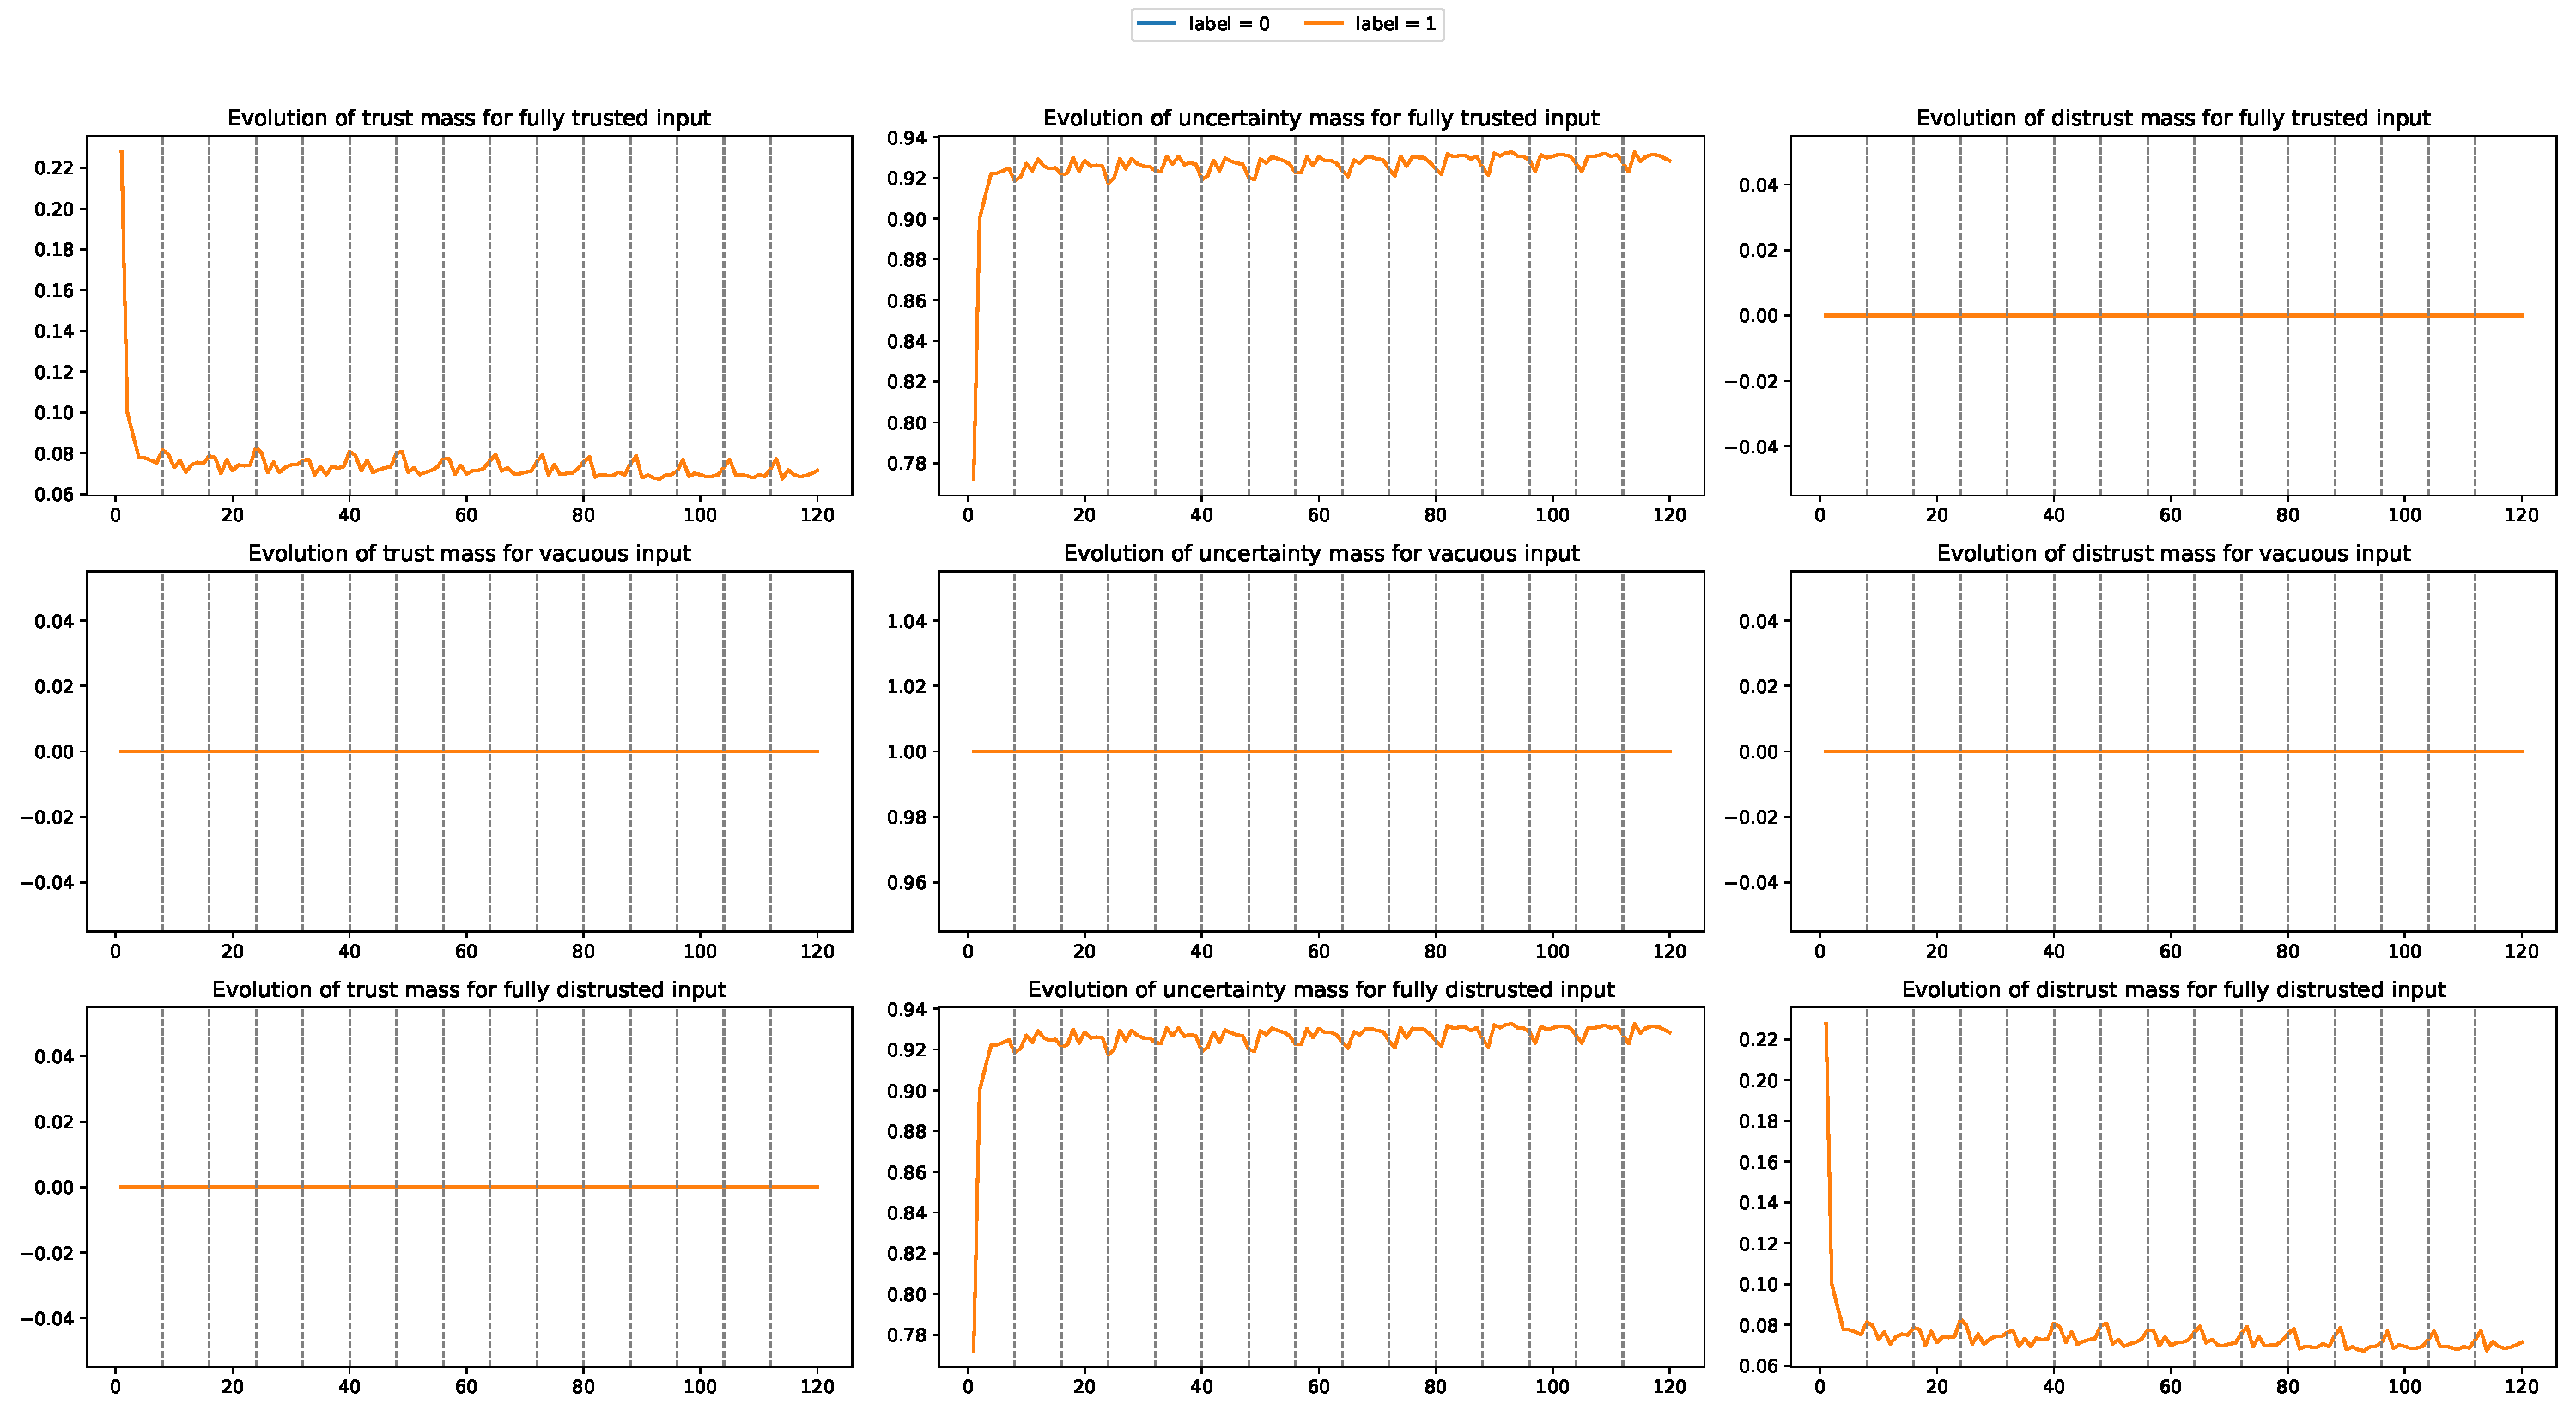
\includegraphics[width=0.8\textwidth]{latex/PTAS_Eval_cancer_16_trust_vacuous_eps_0.001_PathSize_None__plot_ptas.pdf}
\caption{cancer\_16\_trust\_vacuous, $\varepsilon$=0.001}
\end{figure}

\begin{figure}[htbp]
\centering
  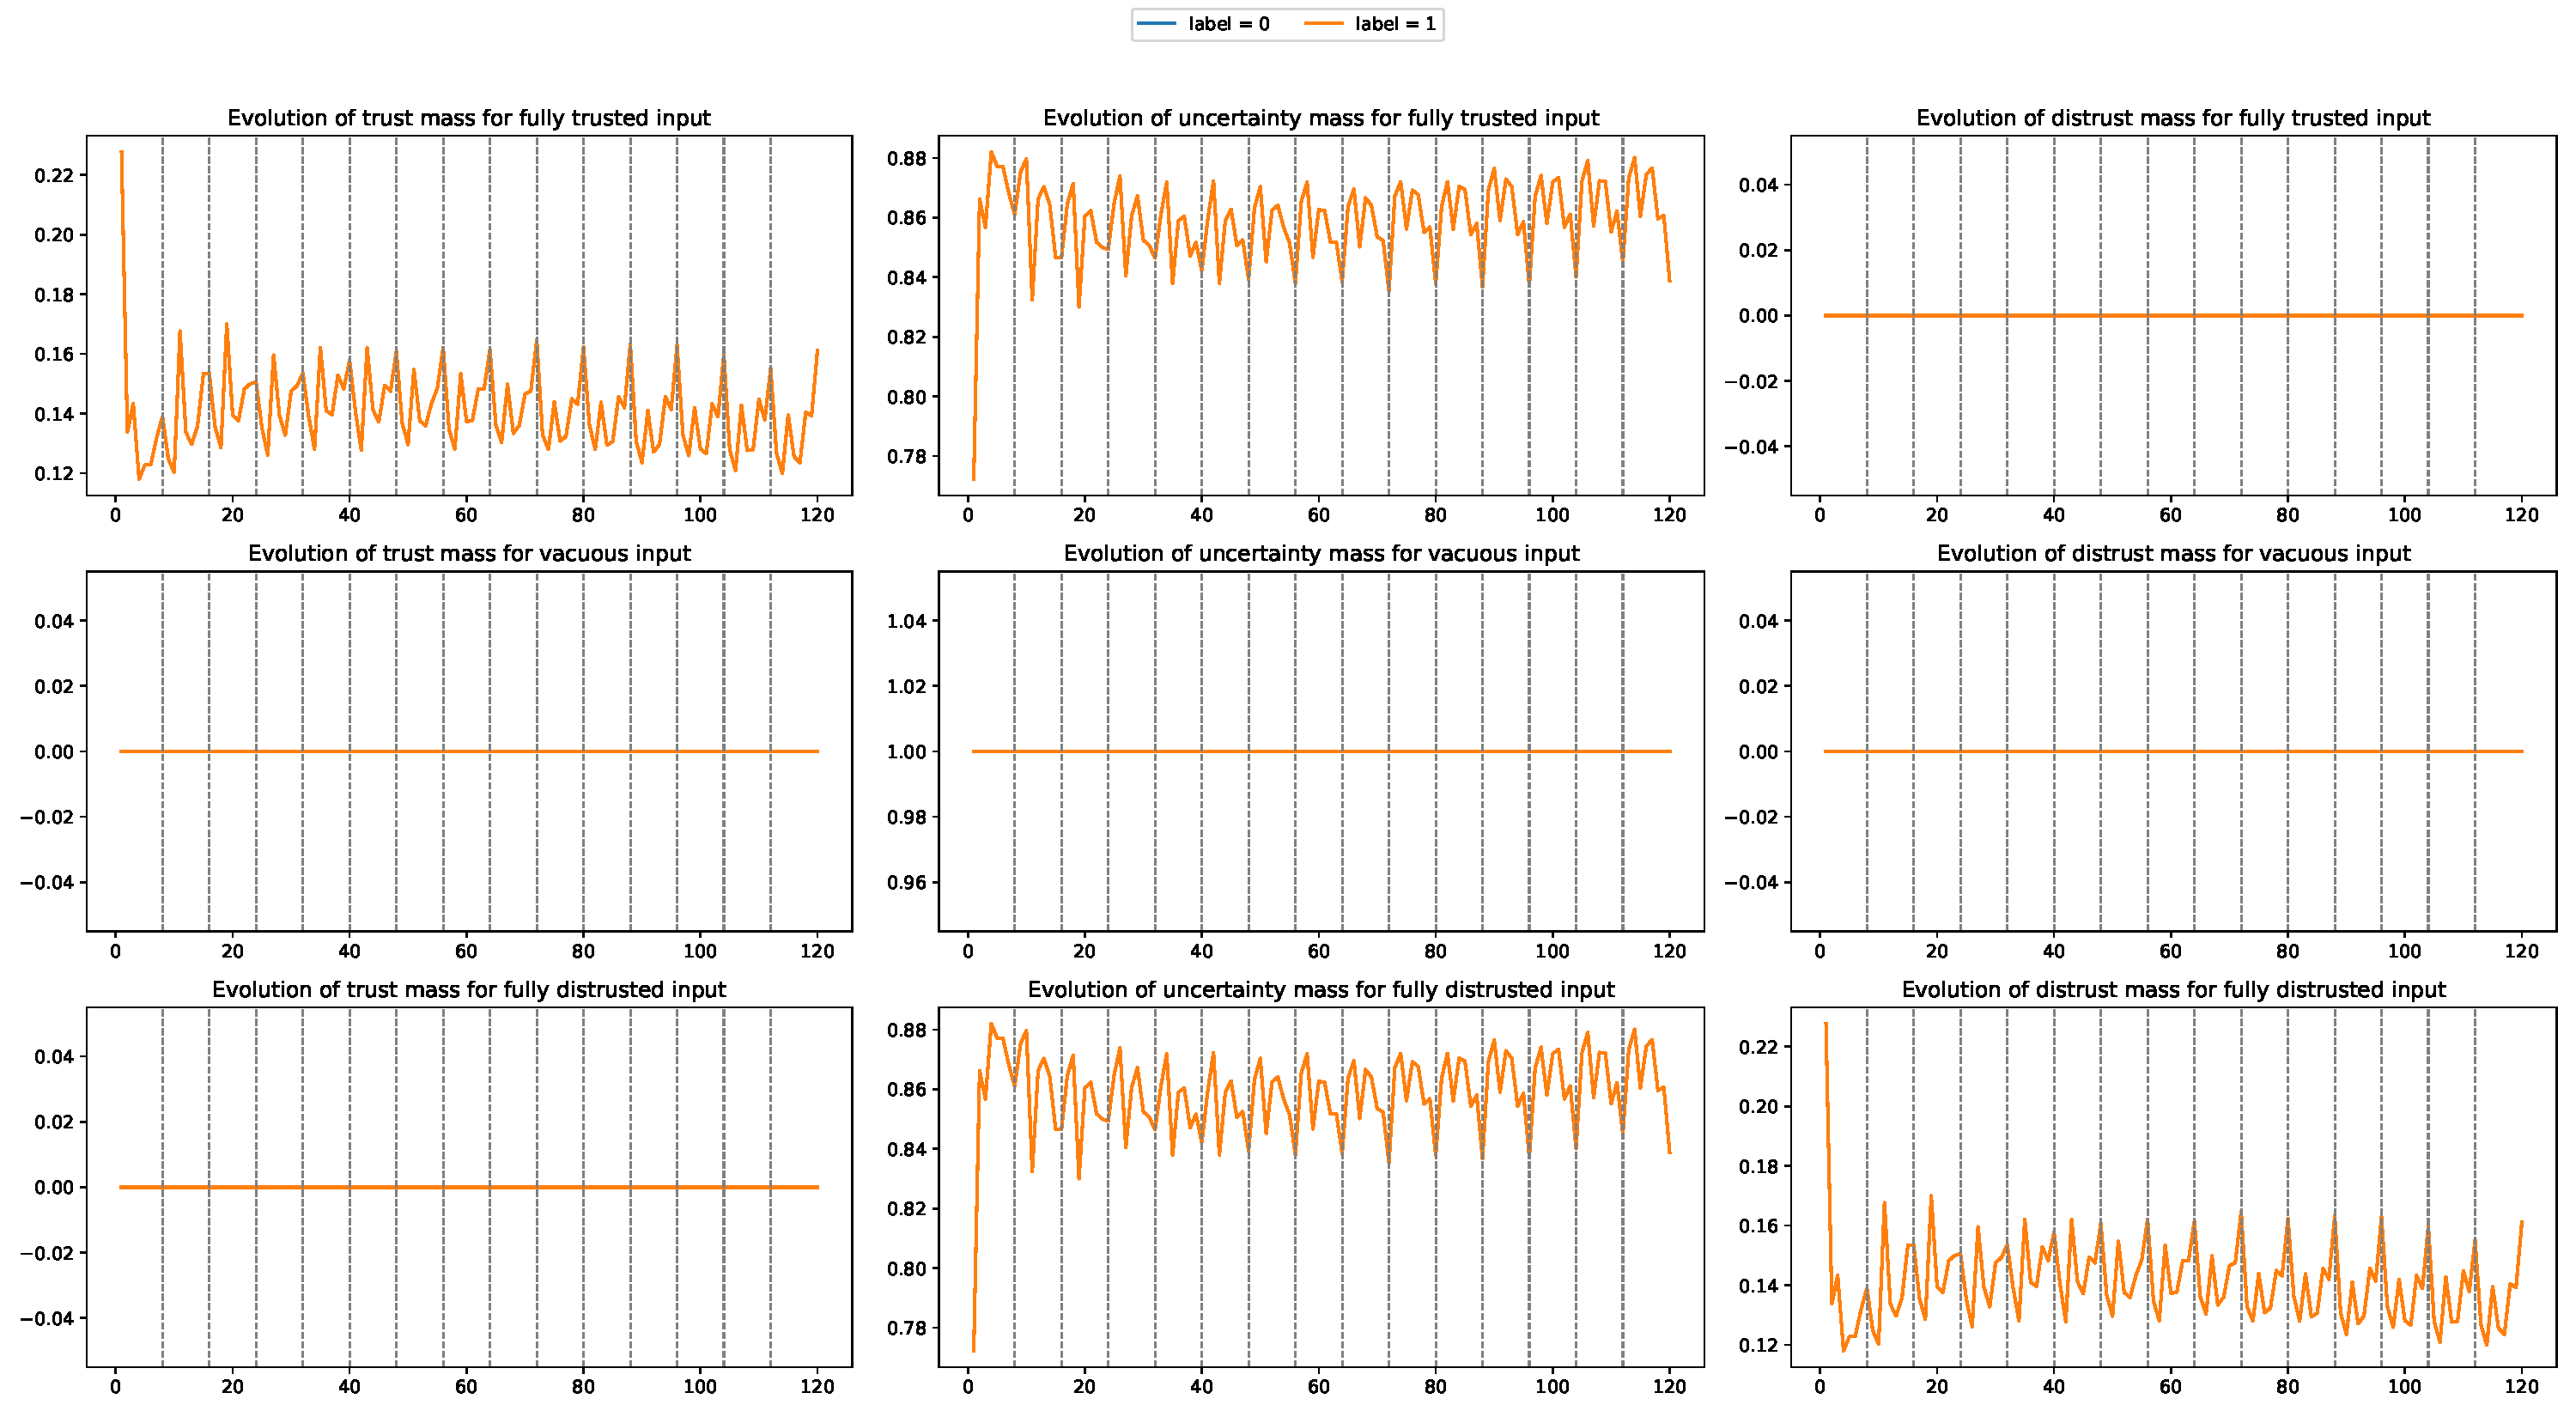
\includegraphics[width=0.8\textwidth]{latex/PTAS_Eval_cancer_16_trust_vacuous_eps_0.01_PathSize_None__plot_ptas.pdf}
\caption{cancer\_16\_trust\_vacuous, $\varepsilon$=0.01}
\end{figure}

\begin{figure}[htbp]
\centering
  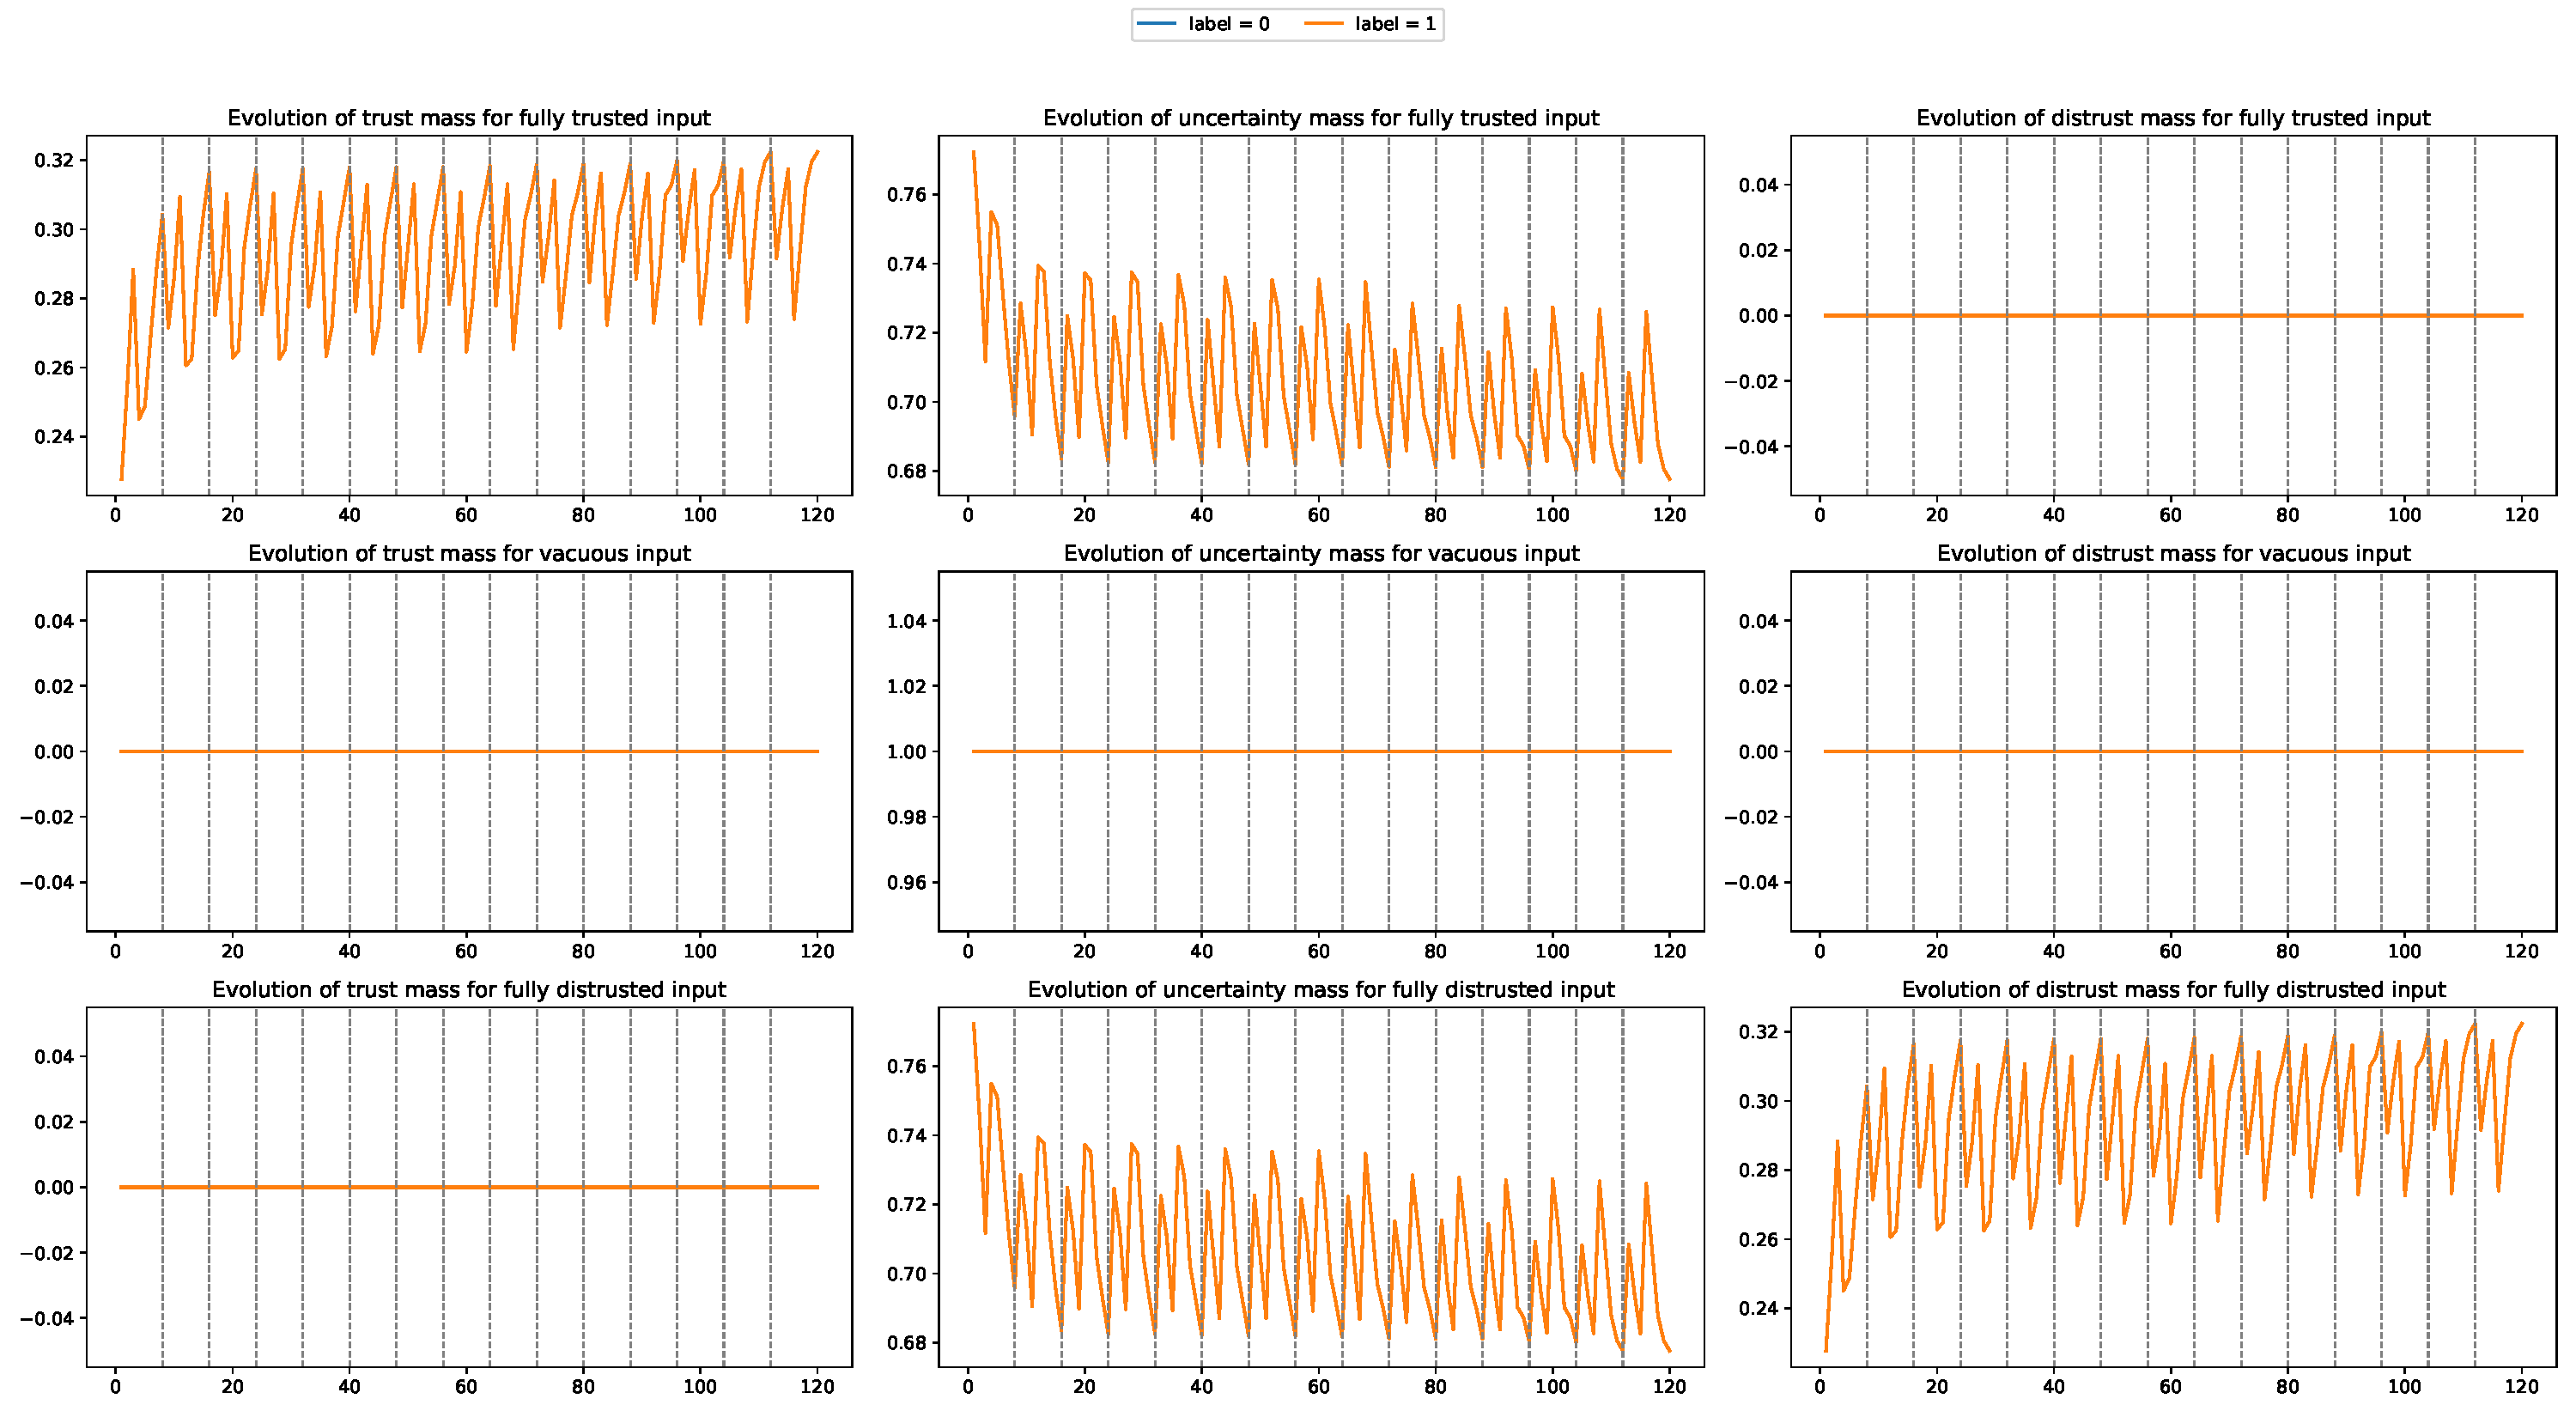
\includegraphics[width=0.8\textwidth]{latex/PTAS_Eval_cancer_16_trust_vacuous_eps_0.1_PathSize_None__plot_ptas.pdf}
\caption{cancer\_16\_trust\_vacuous, $\varepsilon$=0.1}
\end{figure}

\begin{figure}[htbp]
\centering
  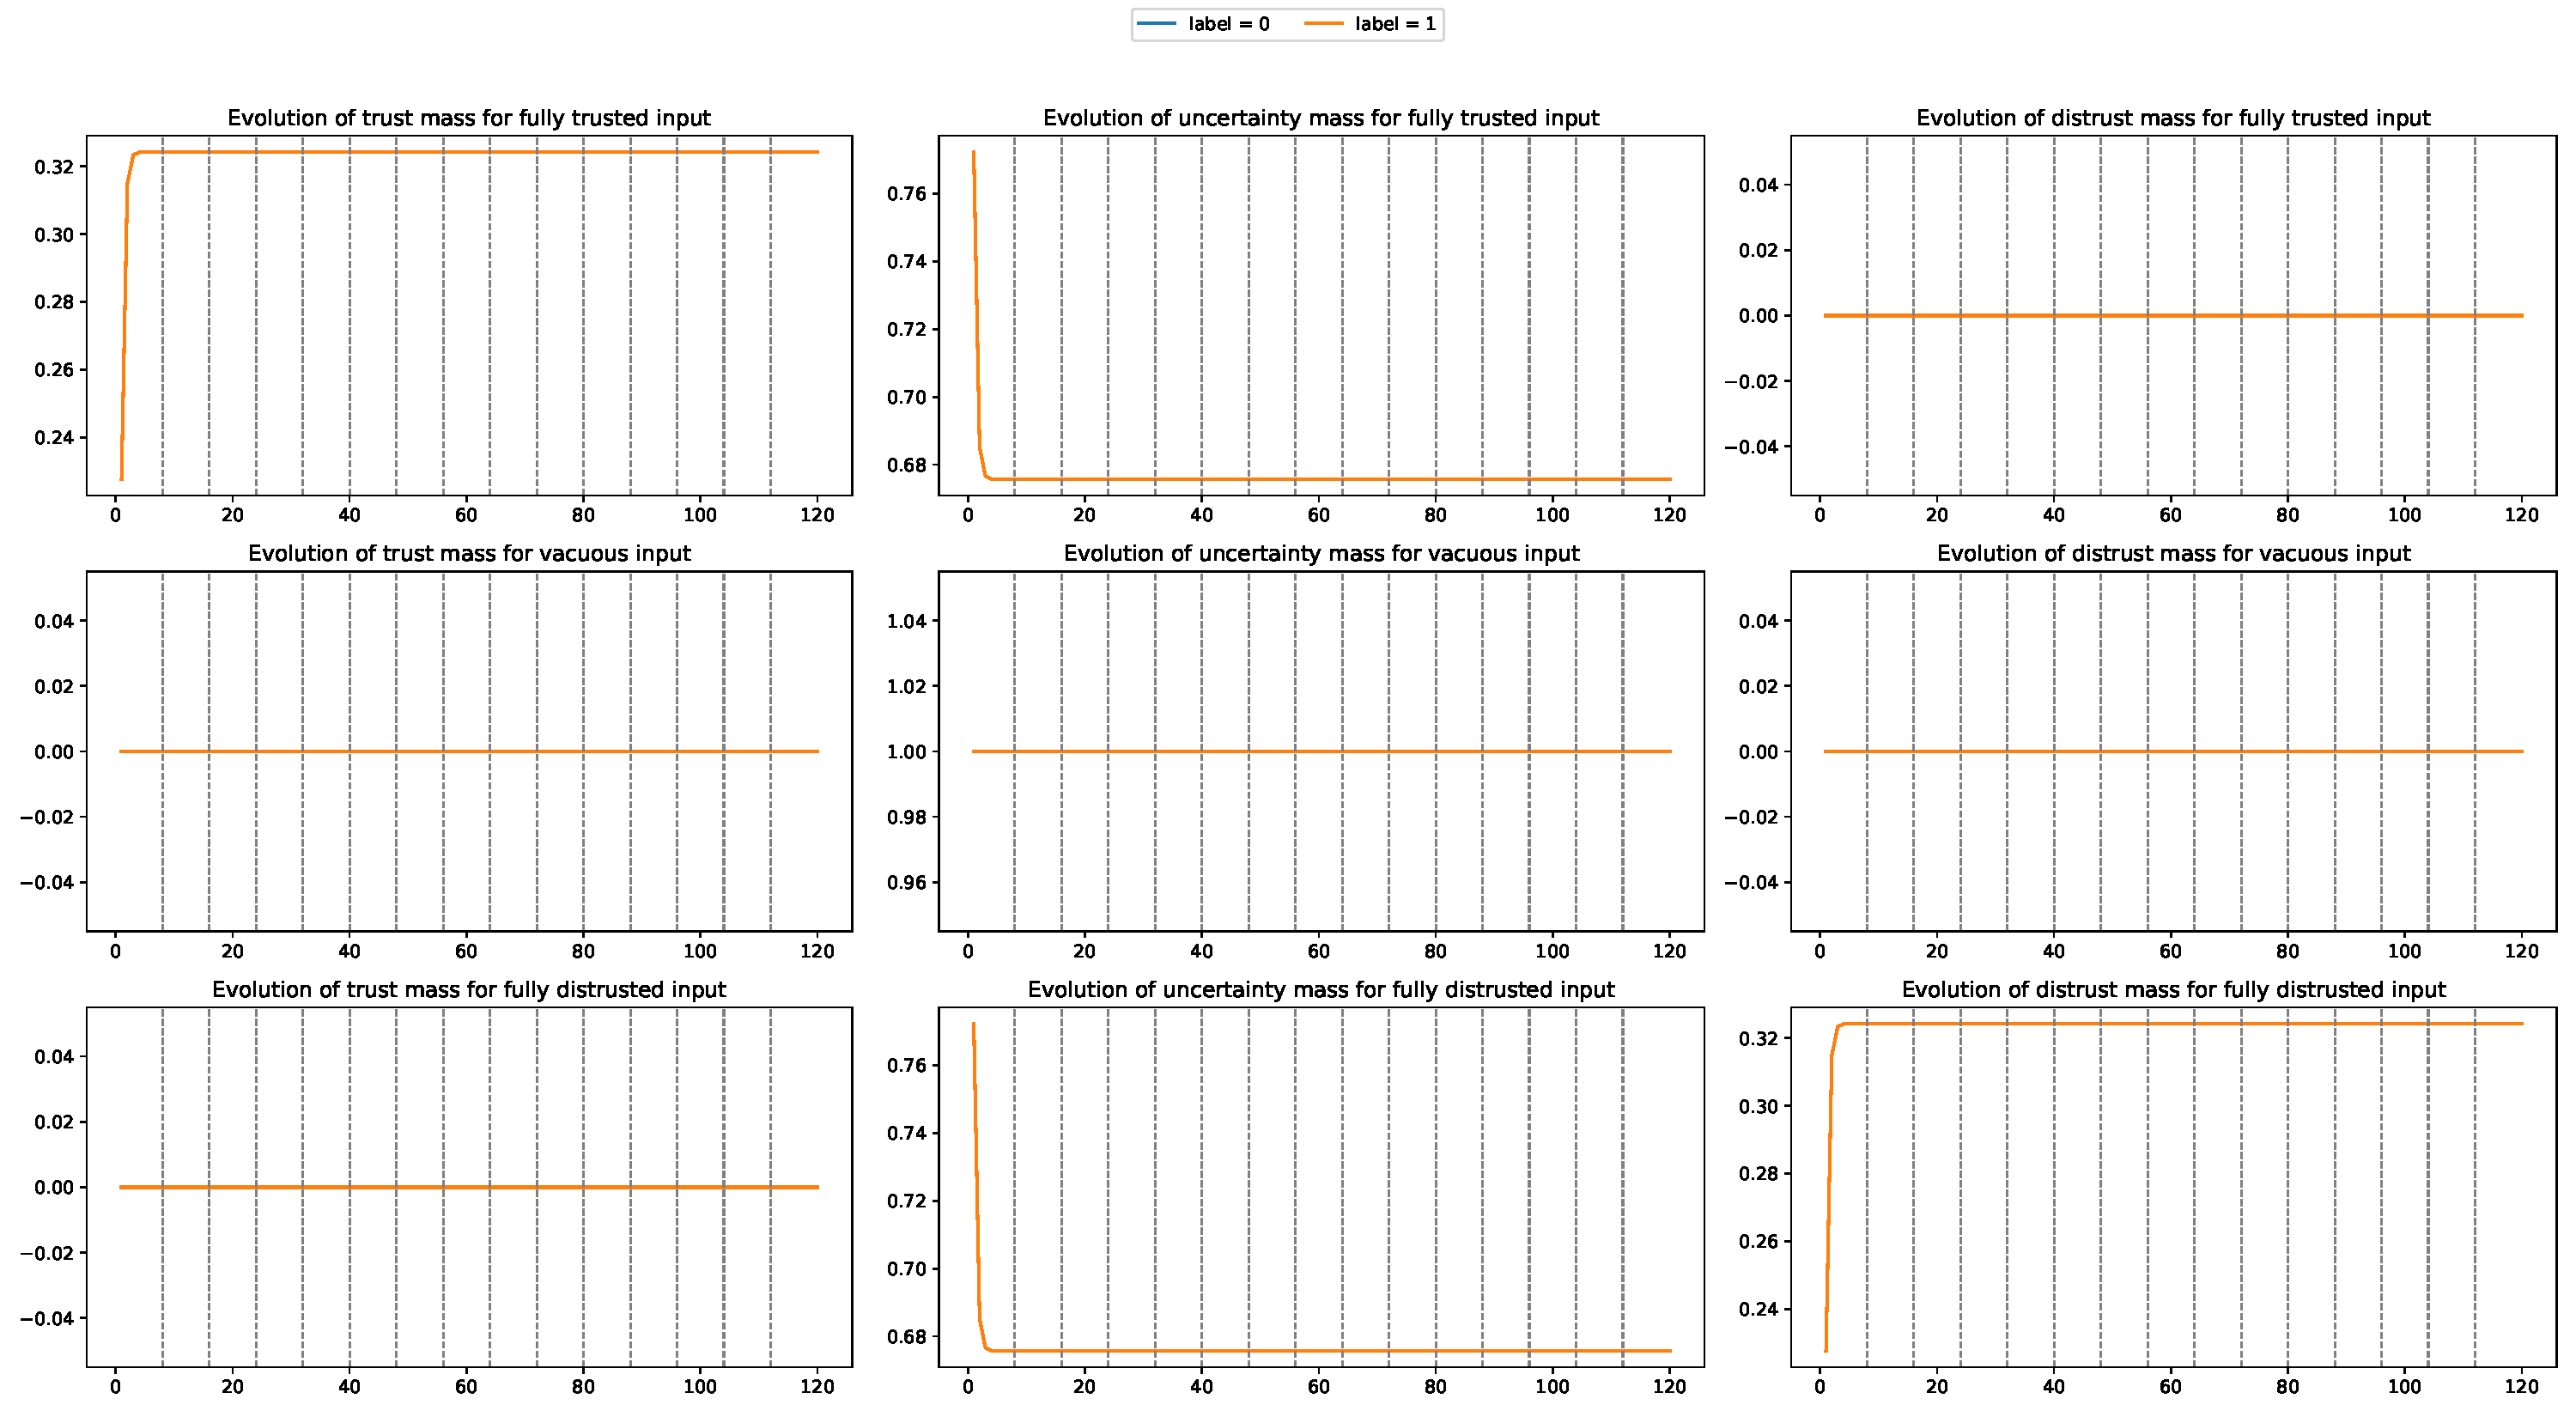
\includegraphics[width=0.8\textwidth]{latex/PTAS_Eval_cancer_16_trust_vacuous_eps_1_PathSize_None__plot_ptas.pdf}
\caption{cancer\_16\_trust\_vacuous, $\varepsilon$=1}
\end{figure}

\subsubsection{vacuous -- distrust}

\begin{figure}[htbp]
\centering
  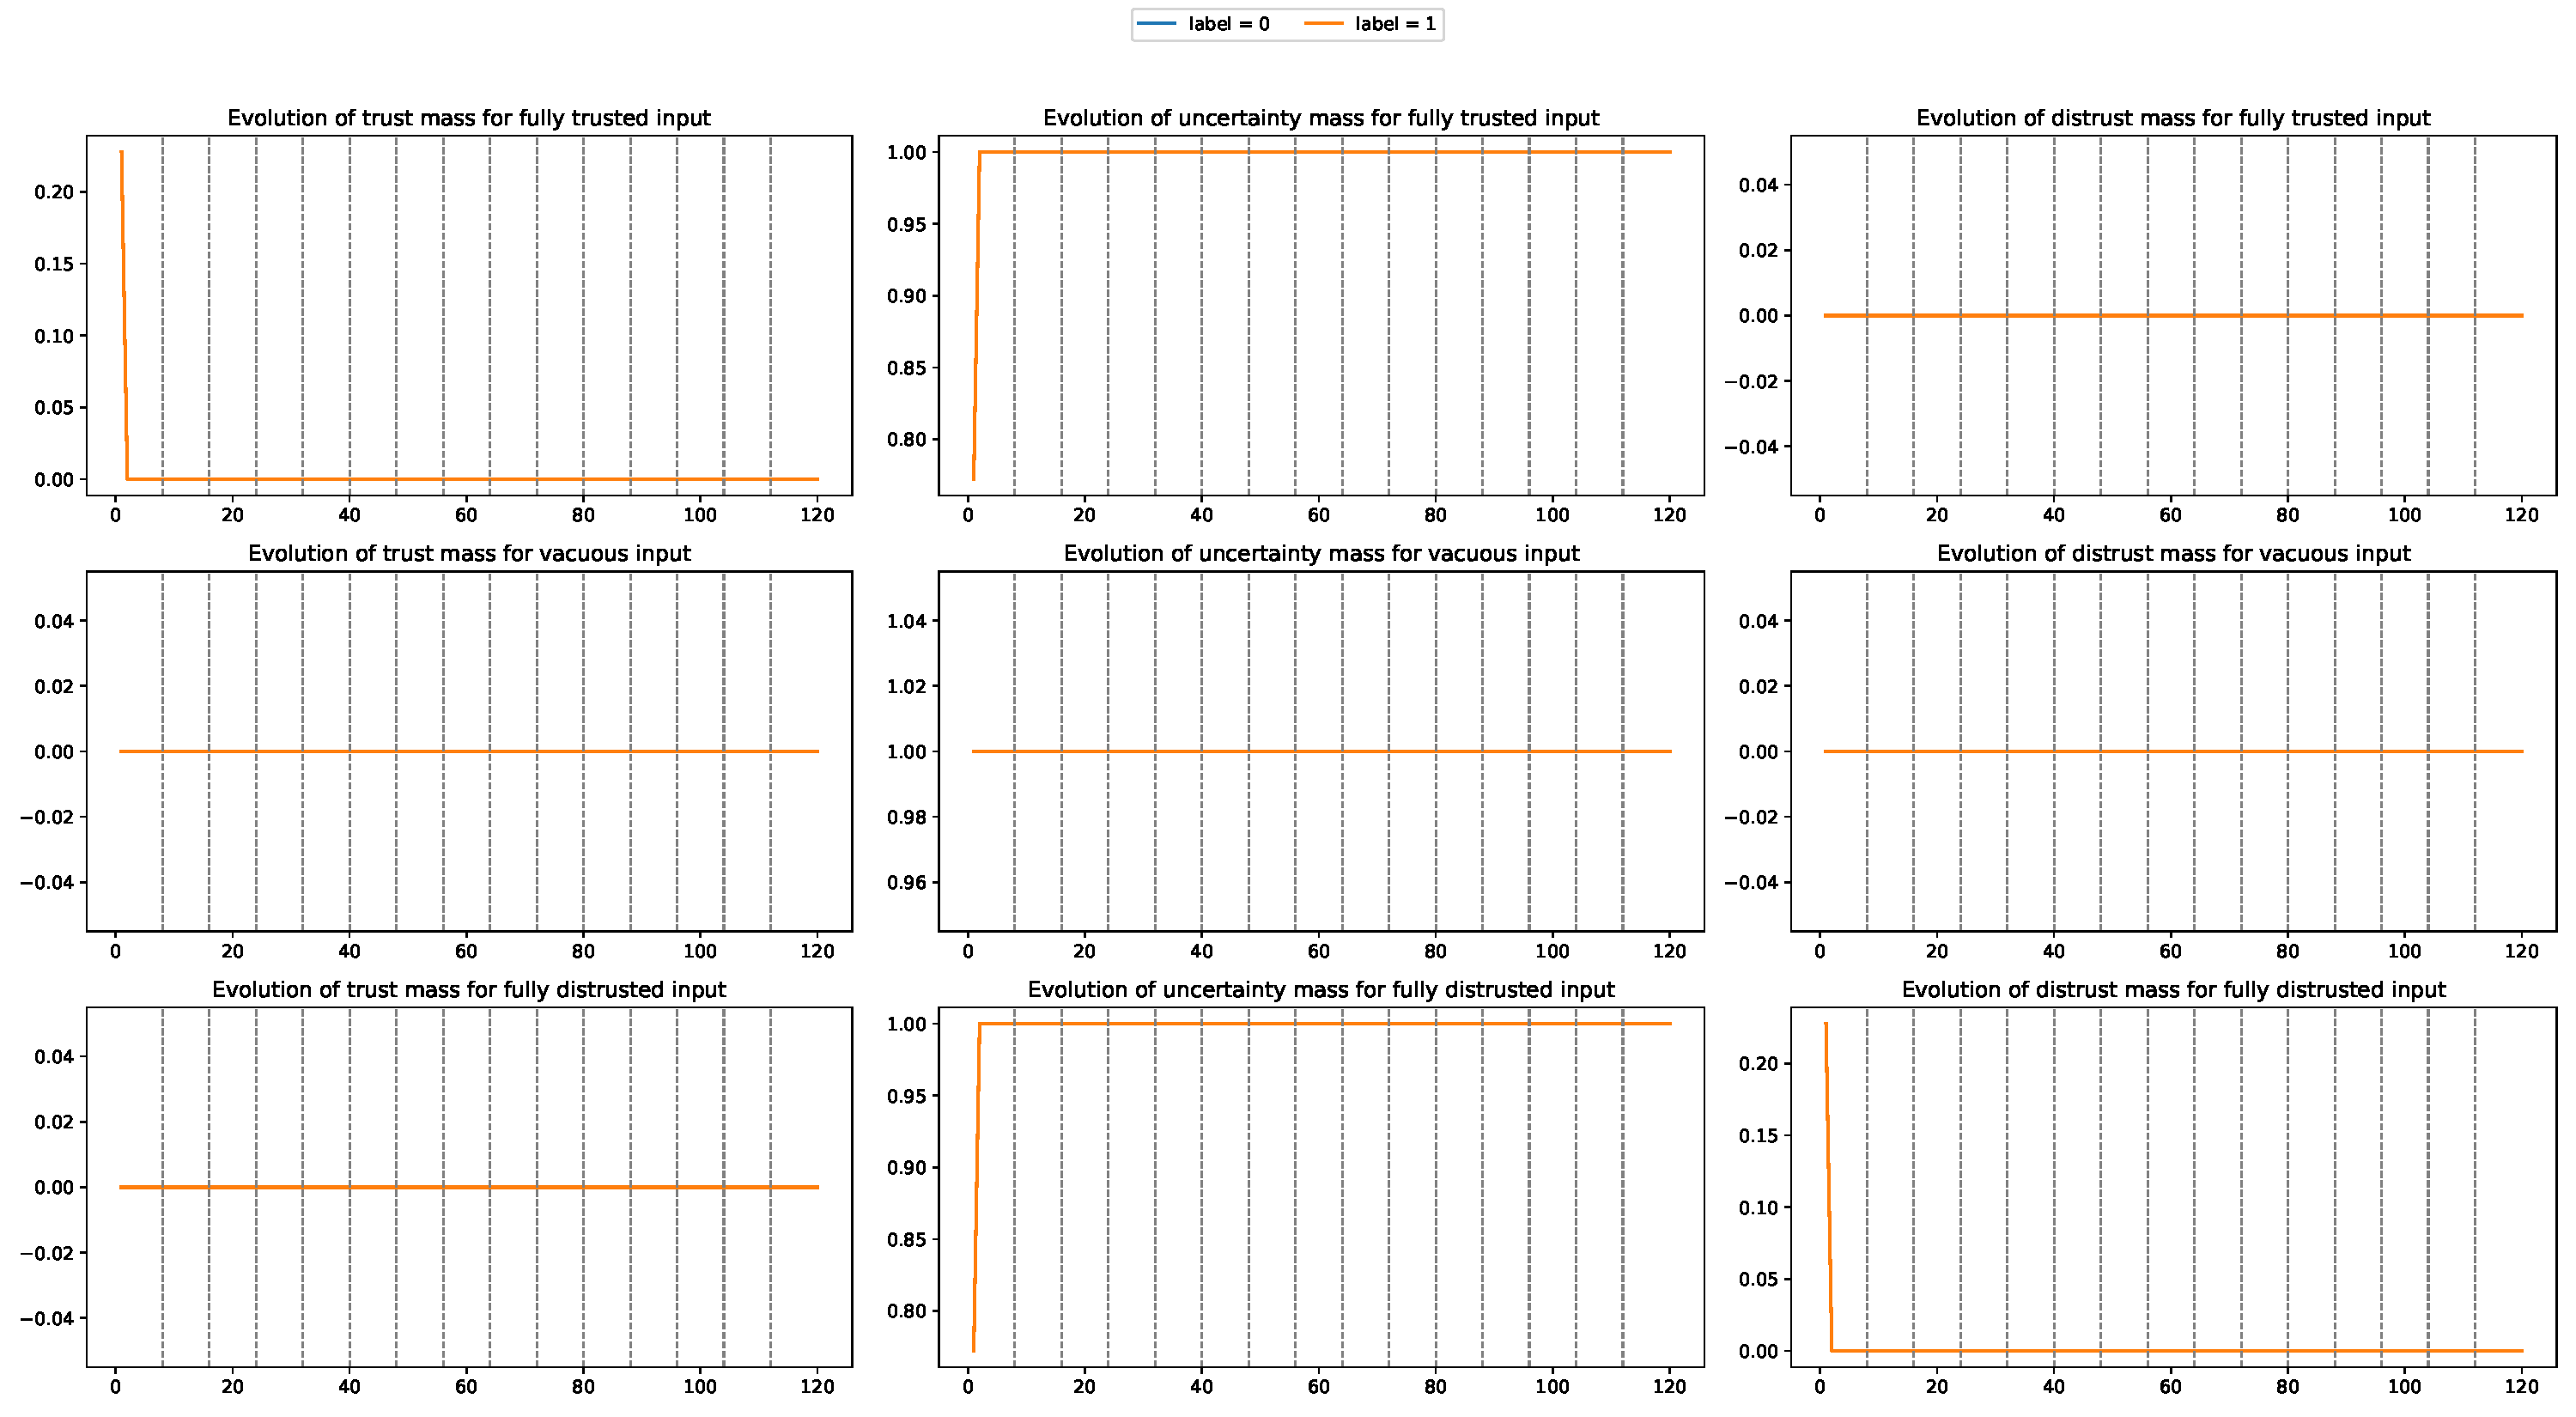
\includegraphics[width=0.8\textwidth]{latex/PTAS_Eval_cancer_16_vacuous_distrust_eps_0.001_PathSize_None__plot_ptas.pdf}
\caption{cancer\_16\_vacuous\_distrust, $\varepsilon$=0.001}
\end{figure}

\begin{figure}[htbp]
\centering
  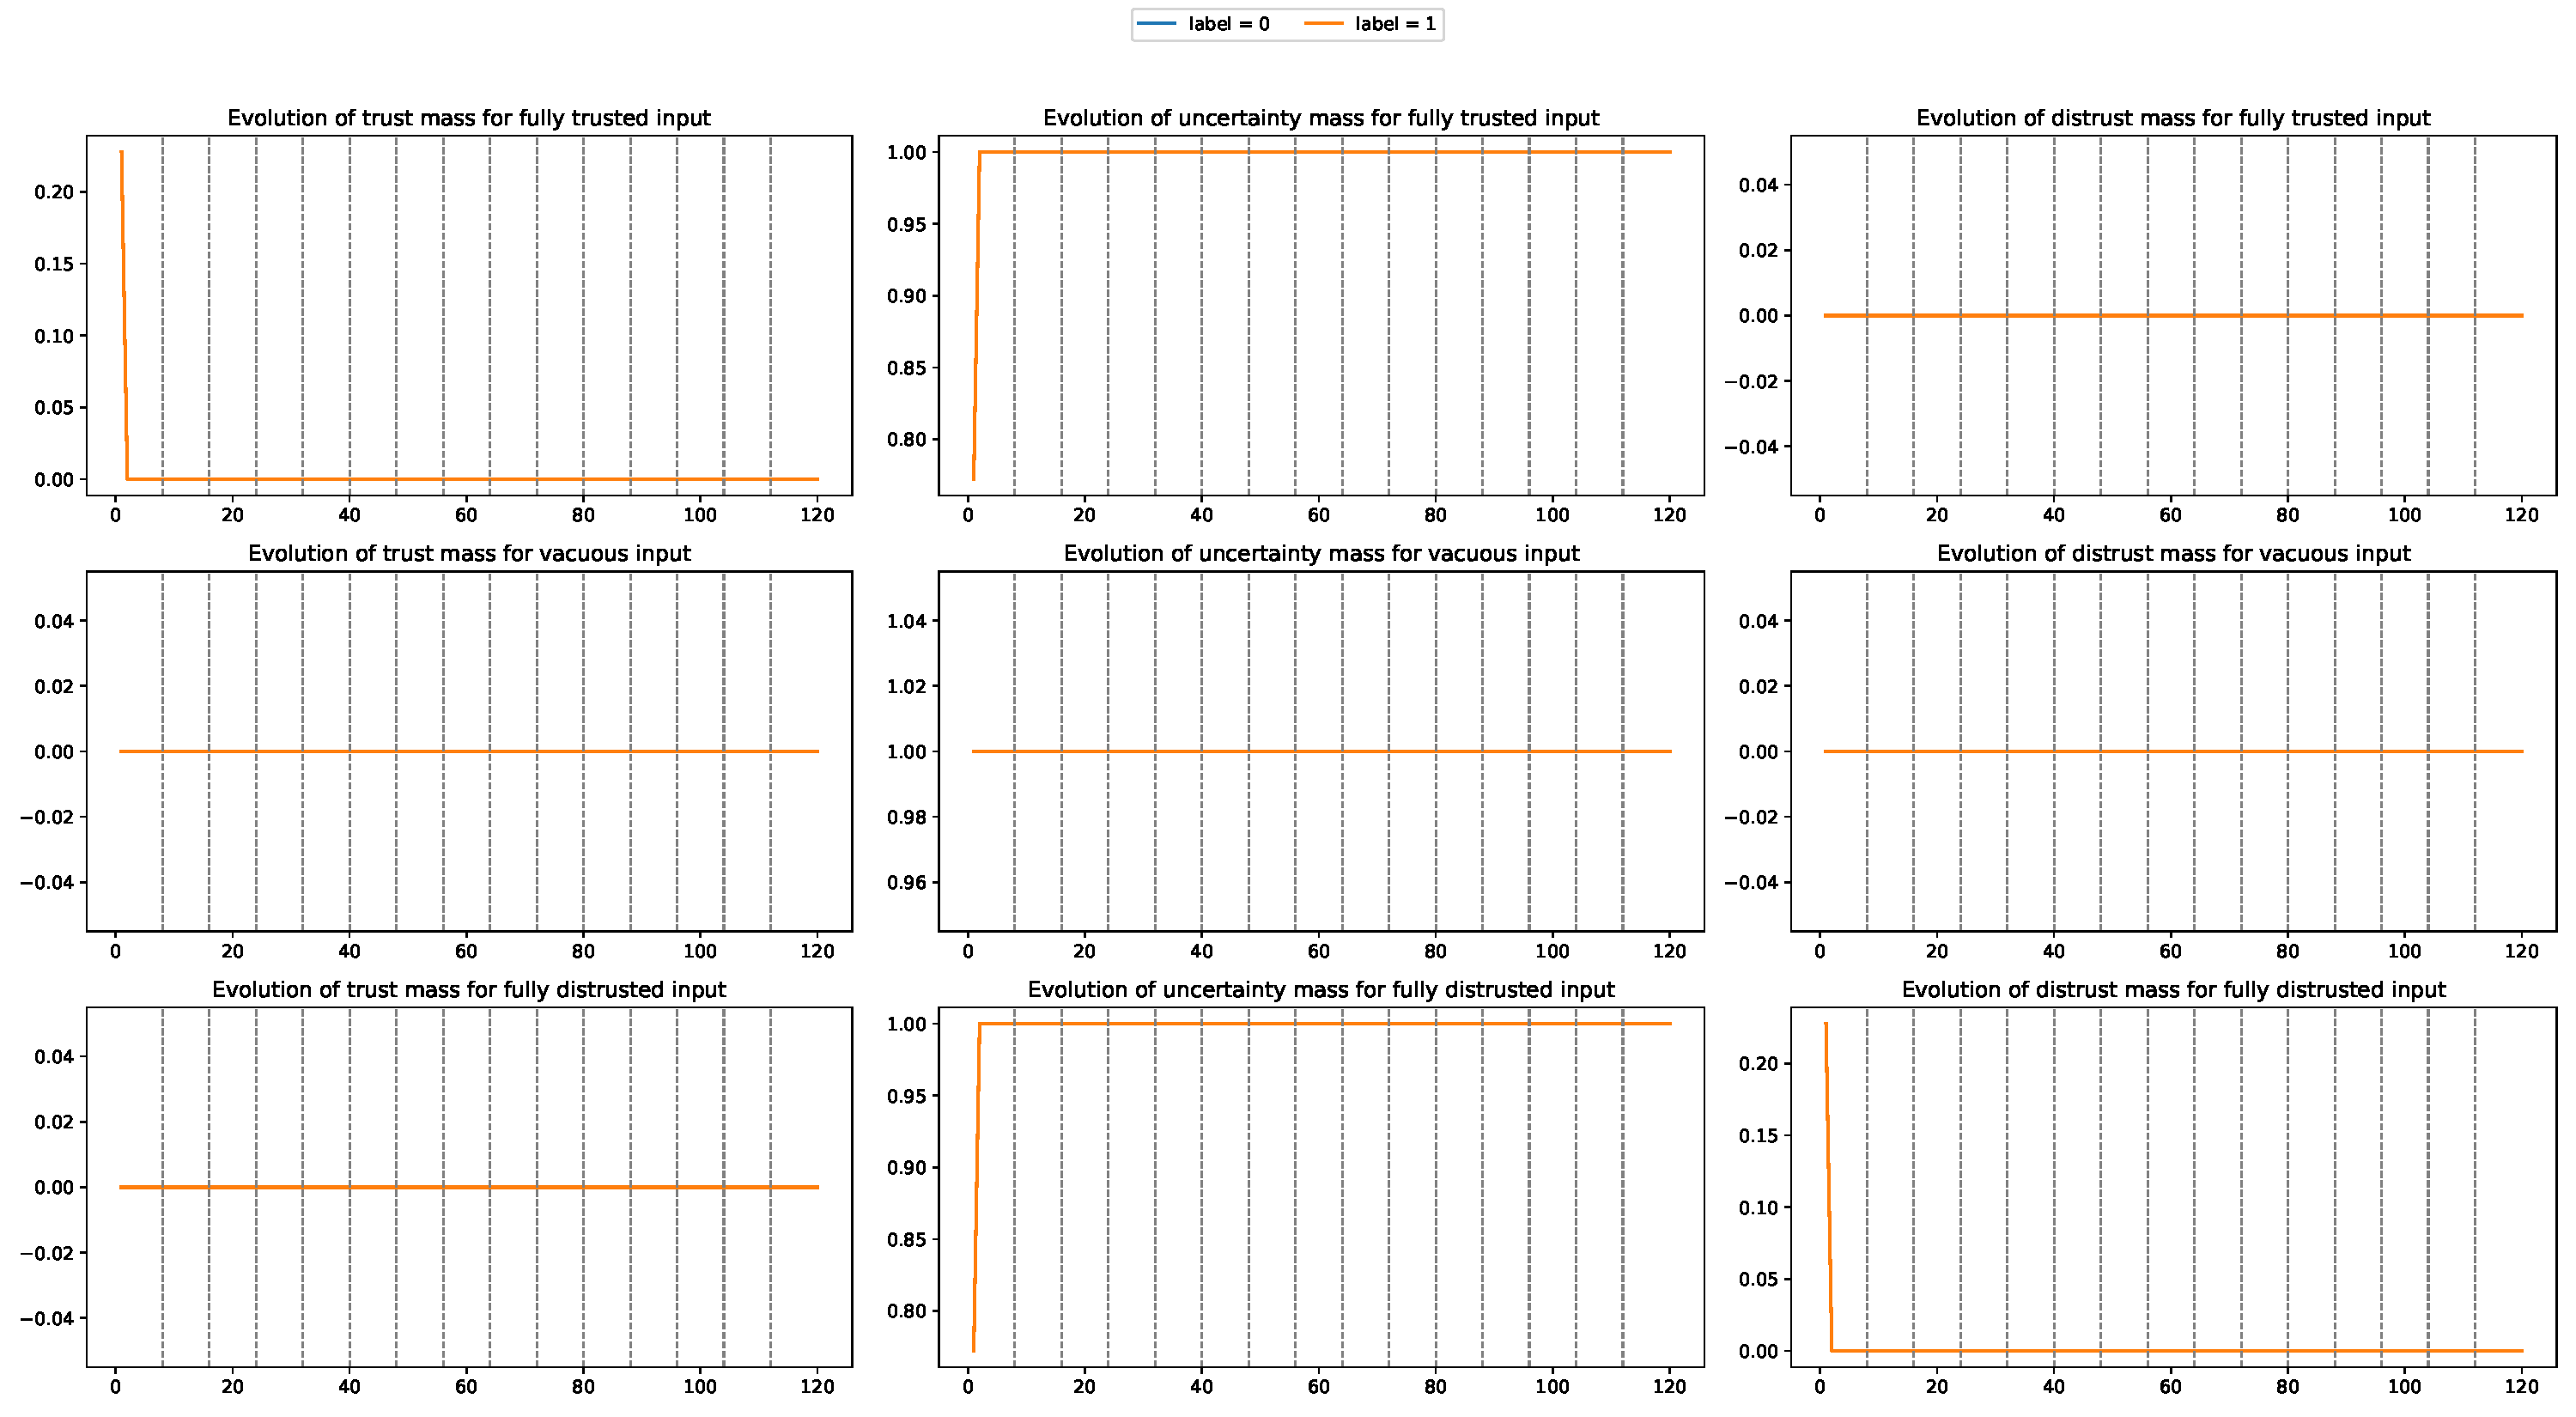
\includegraphics[width=0.8\textwidth]{latex/PTAS_Eval_cancer_16_vacuous_distrust_eps_0.01_PathSize_None__plot_ptas.pdf}
\caption{cancer\_16\_vacuous\_distrust, $\varepsilon$=0.01}
\end{figure}

\begin{figure}[htbp]
\centering
  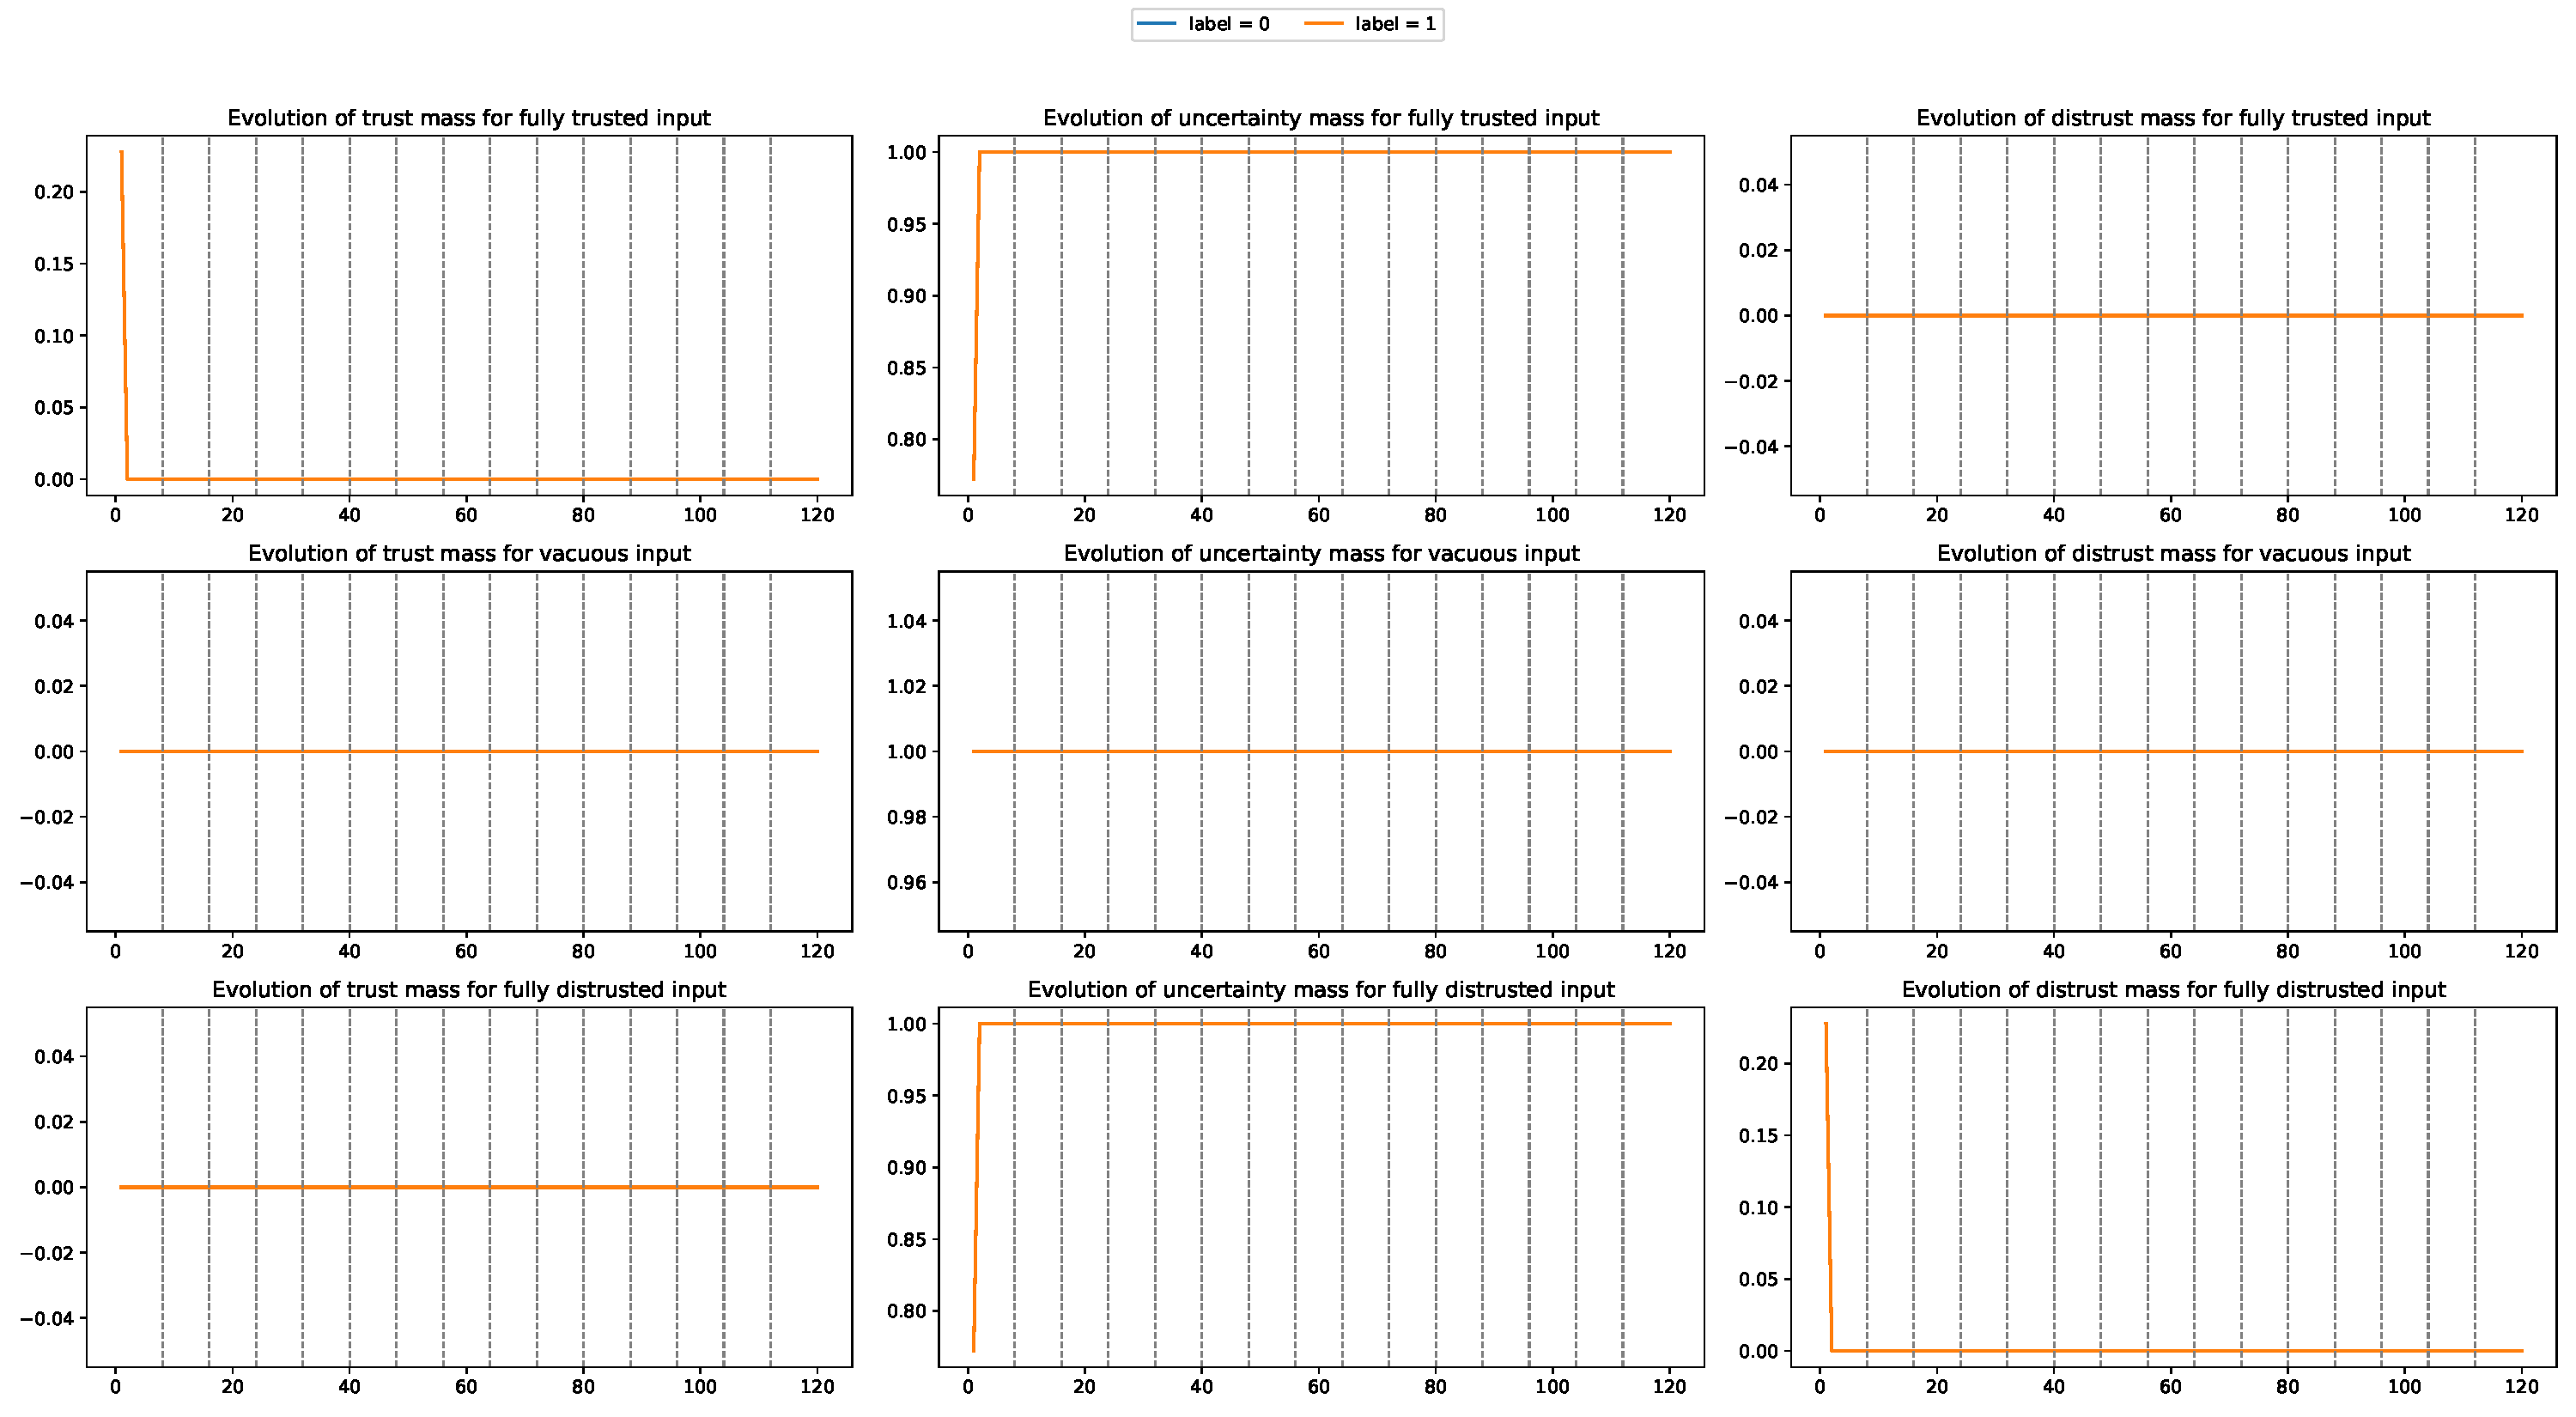
\includegraphics[width=0.8\textwidth]{latex/PTAS_Eval_cancer_16_vacuous_distrust_eps_0.1_PathSize_None__plot_ptas.pdf}
\caption{cancer\_16\_vacuous\_distrust, $\varepsilon$=0.1}
\end{figure}

\begin{figure}[htbp]
\centering
  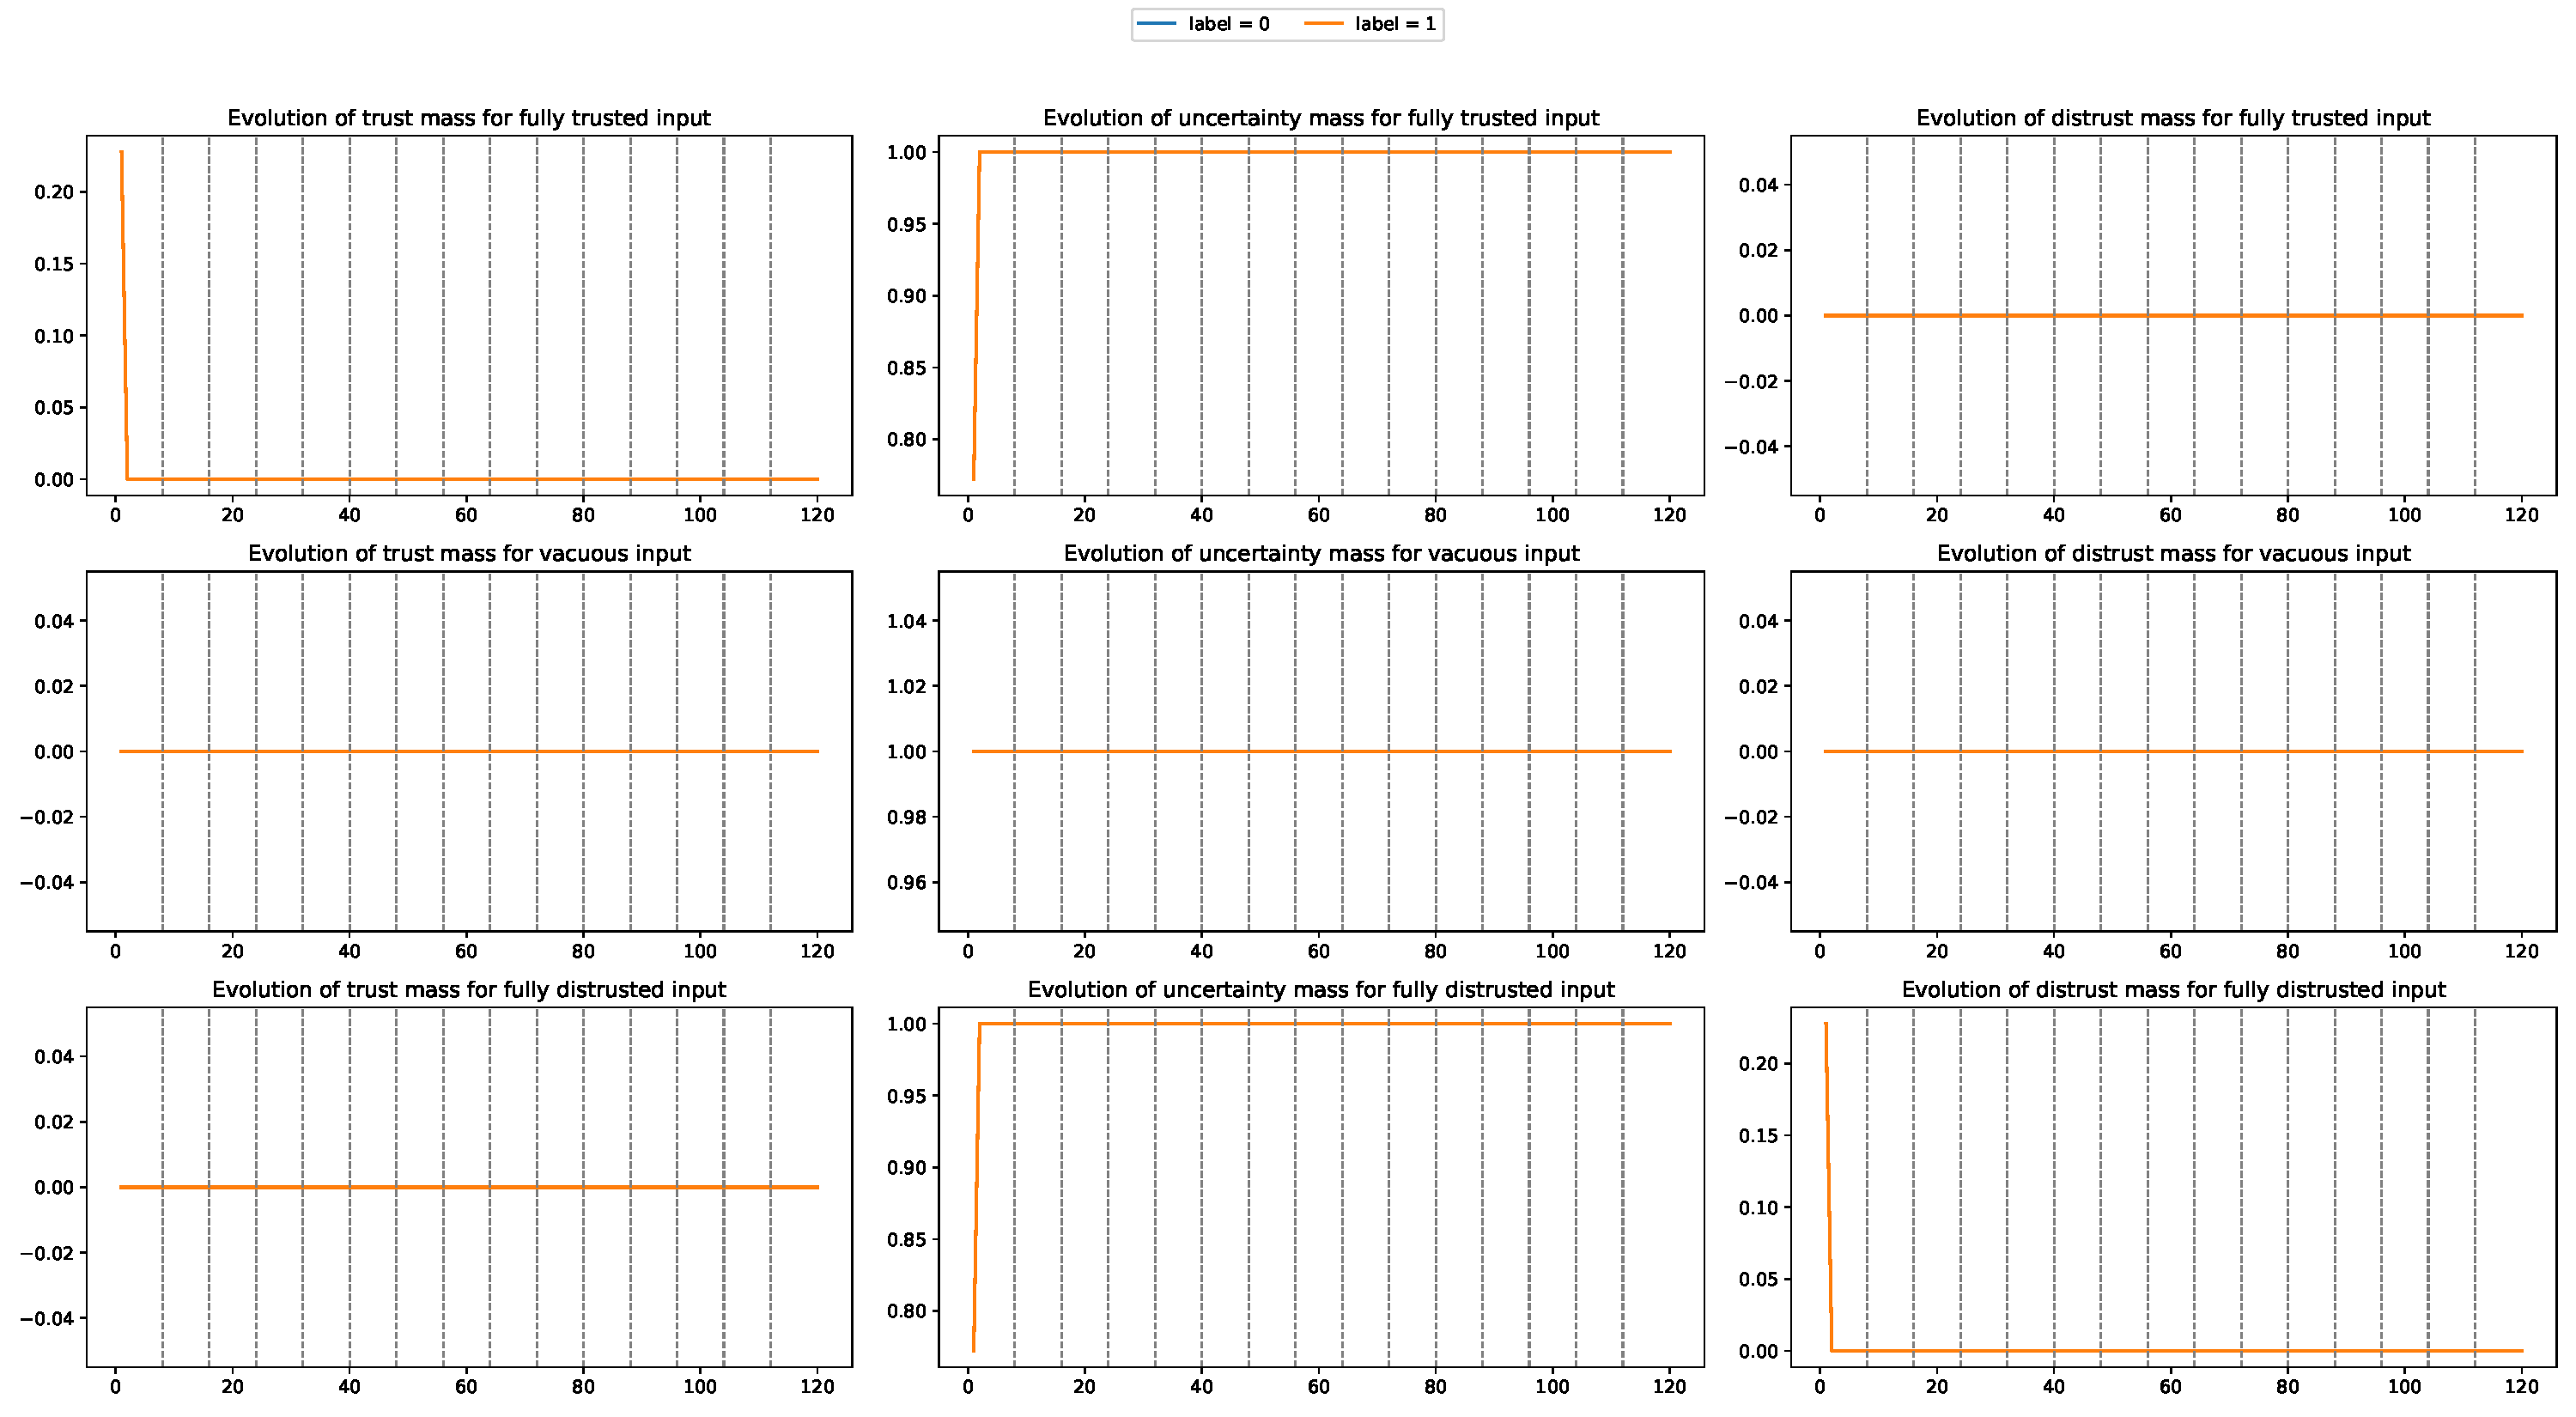
\includegraphics[width=0.8\textwidth]{latex/PTAS_Eval_cancer_16_vacuous_distrust_eps_1_PathSize_None__plot_ptas.pdf}
\caption{cancer\_16\_vacuous\_distrust, $\varepsilon$=1}
\end{figure}

\subsubsection{vacuous -- trust}

\begin{figure}[htbp]
\centering
  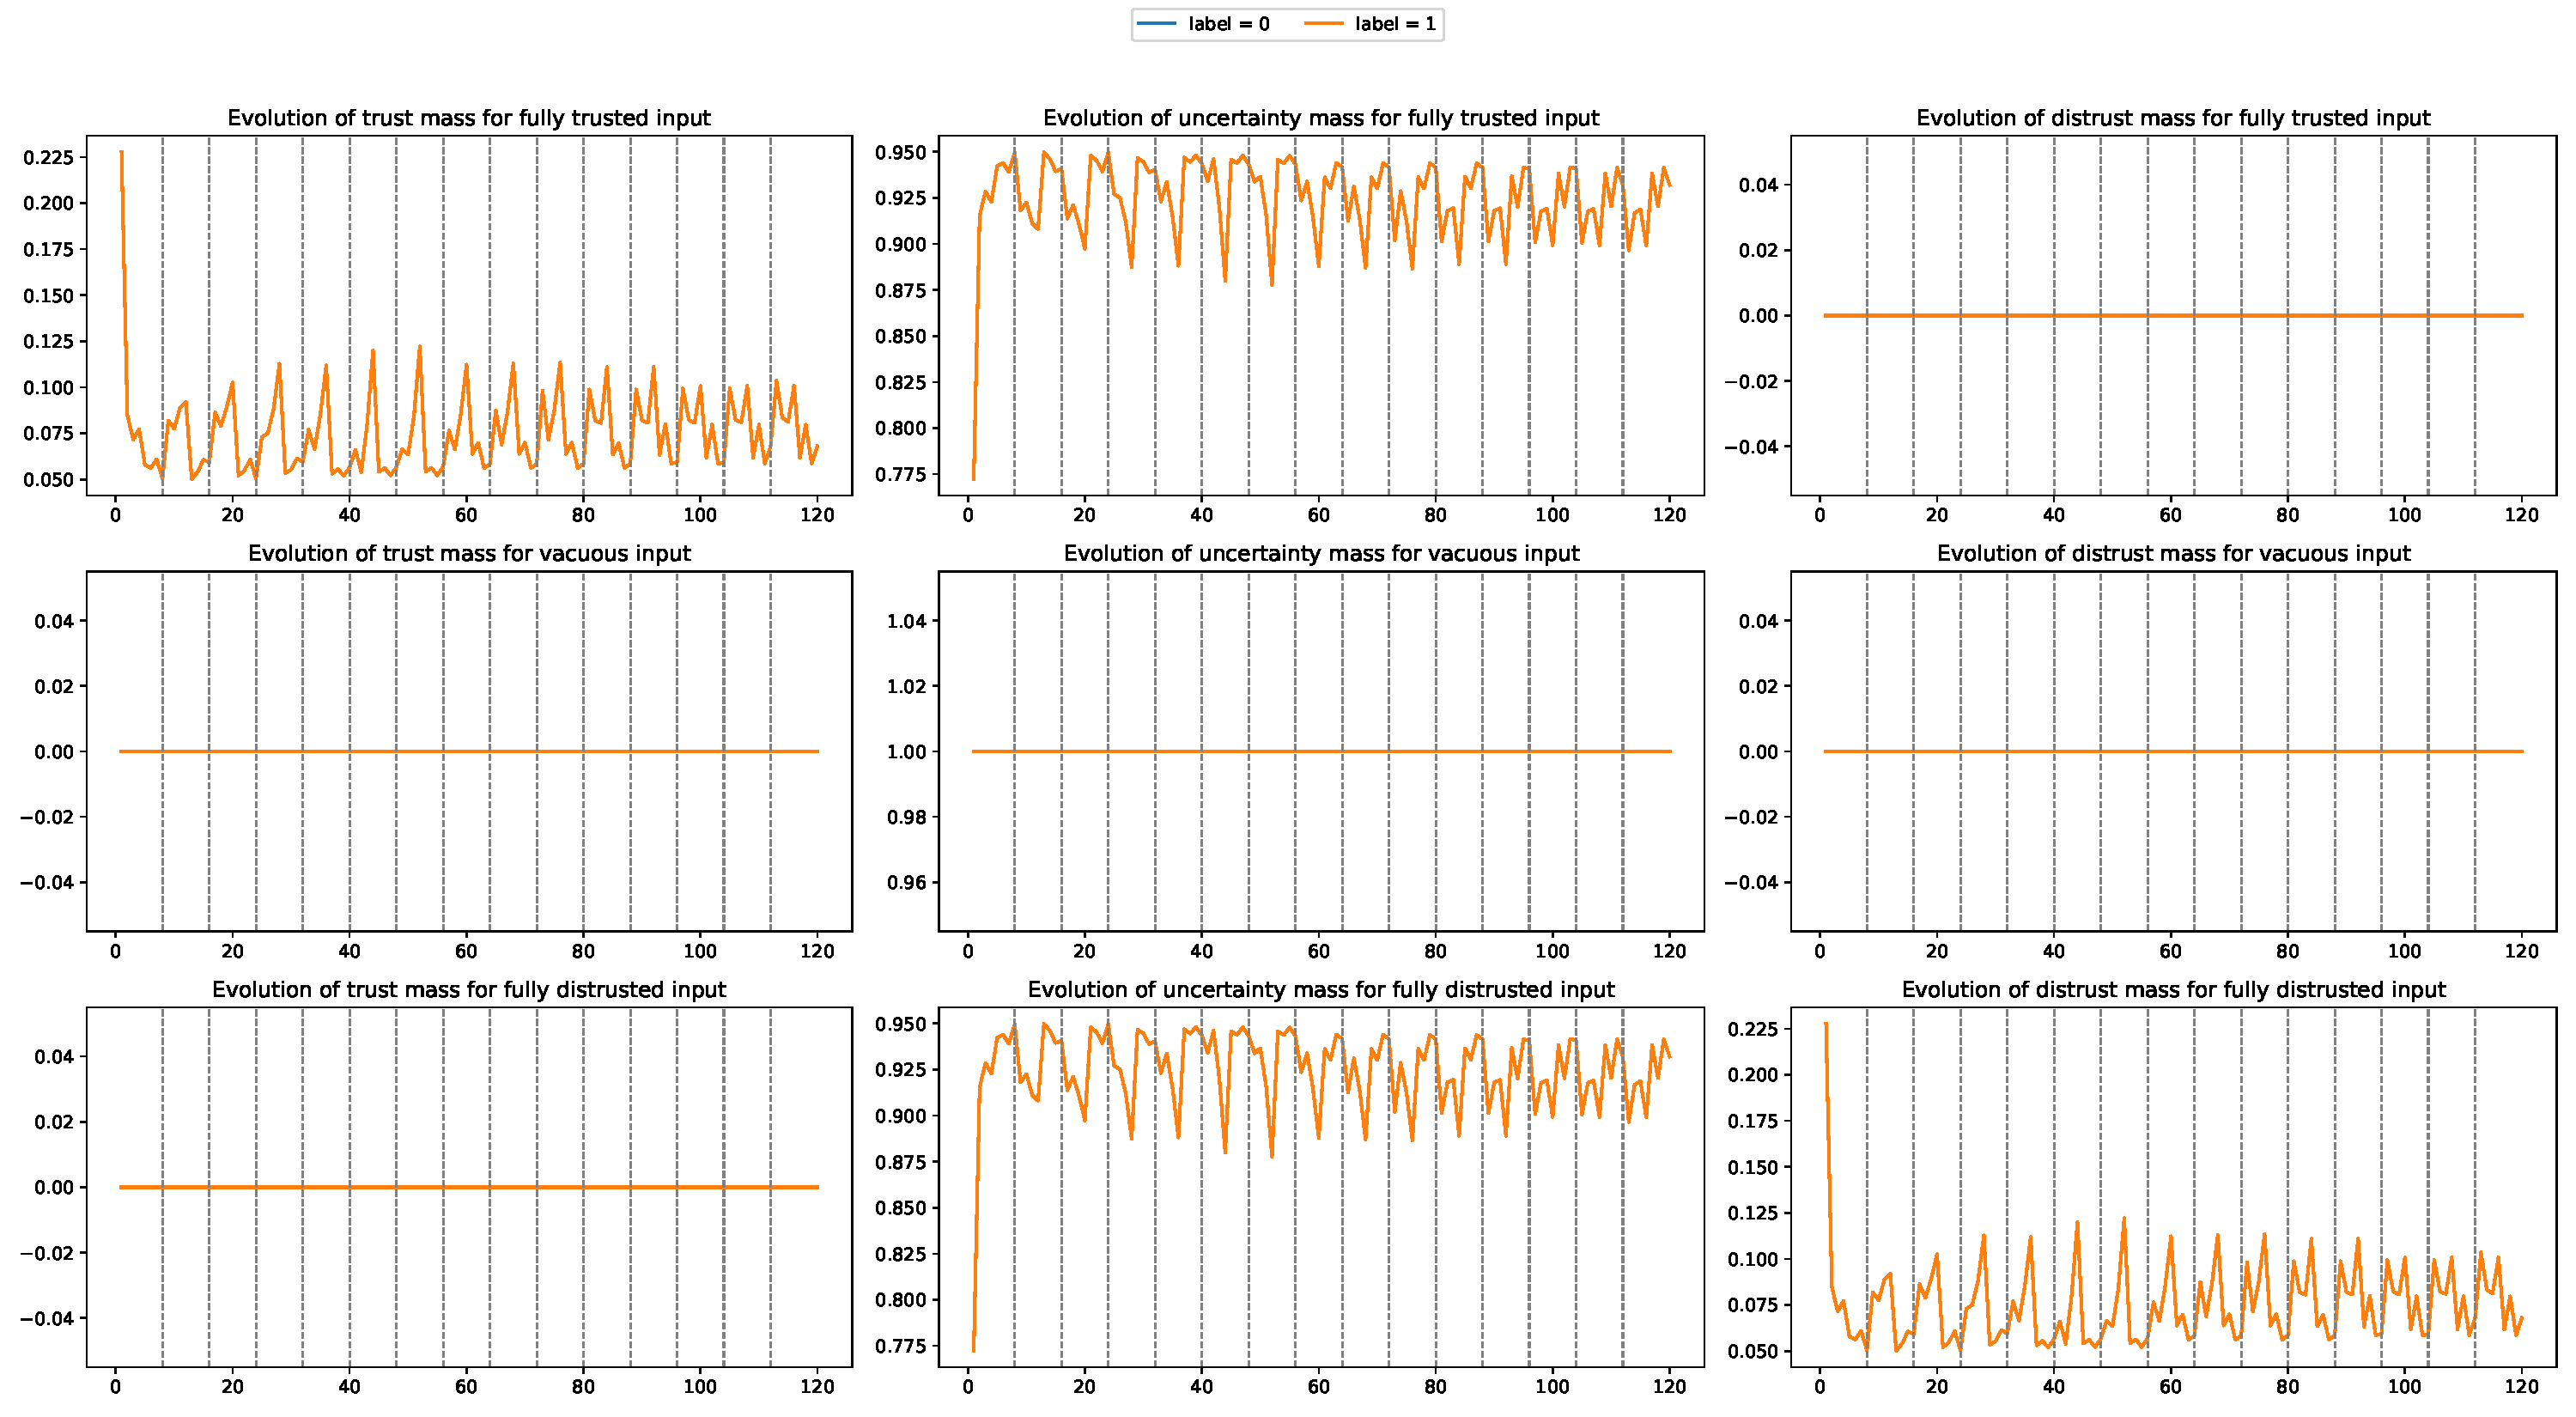
\includegraphics[width=0.8\textwidth]{latex/PTAS_Eval_cancer_16_vacuous_trust_eps_0.001_PathSize_None__plot_ptas.pdf}
\caption{cancer\_16\_vacuous\_trust, $\varepsilon$=0.001}
\end{figure}

\begin{figure}[htbp]
\centering
  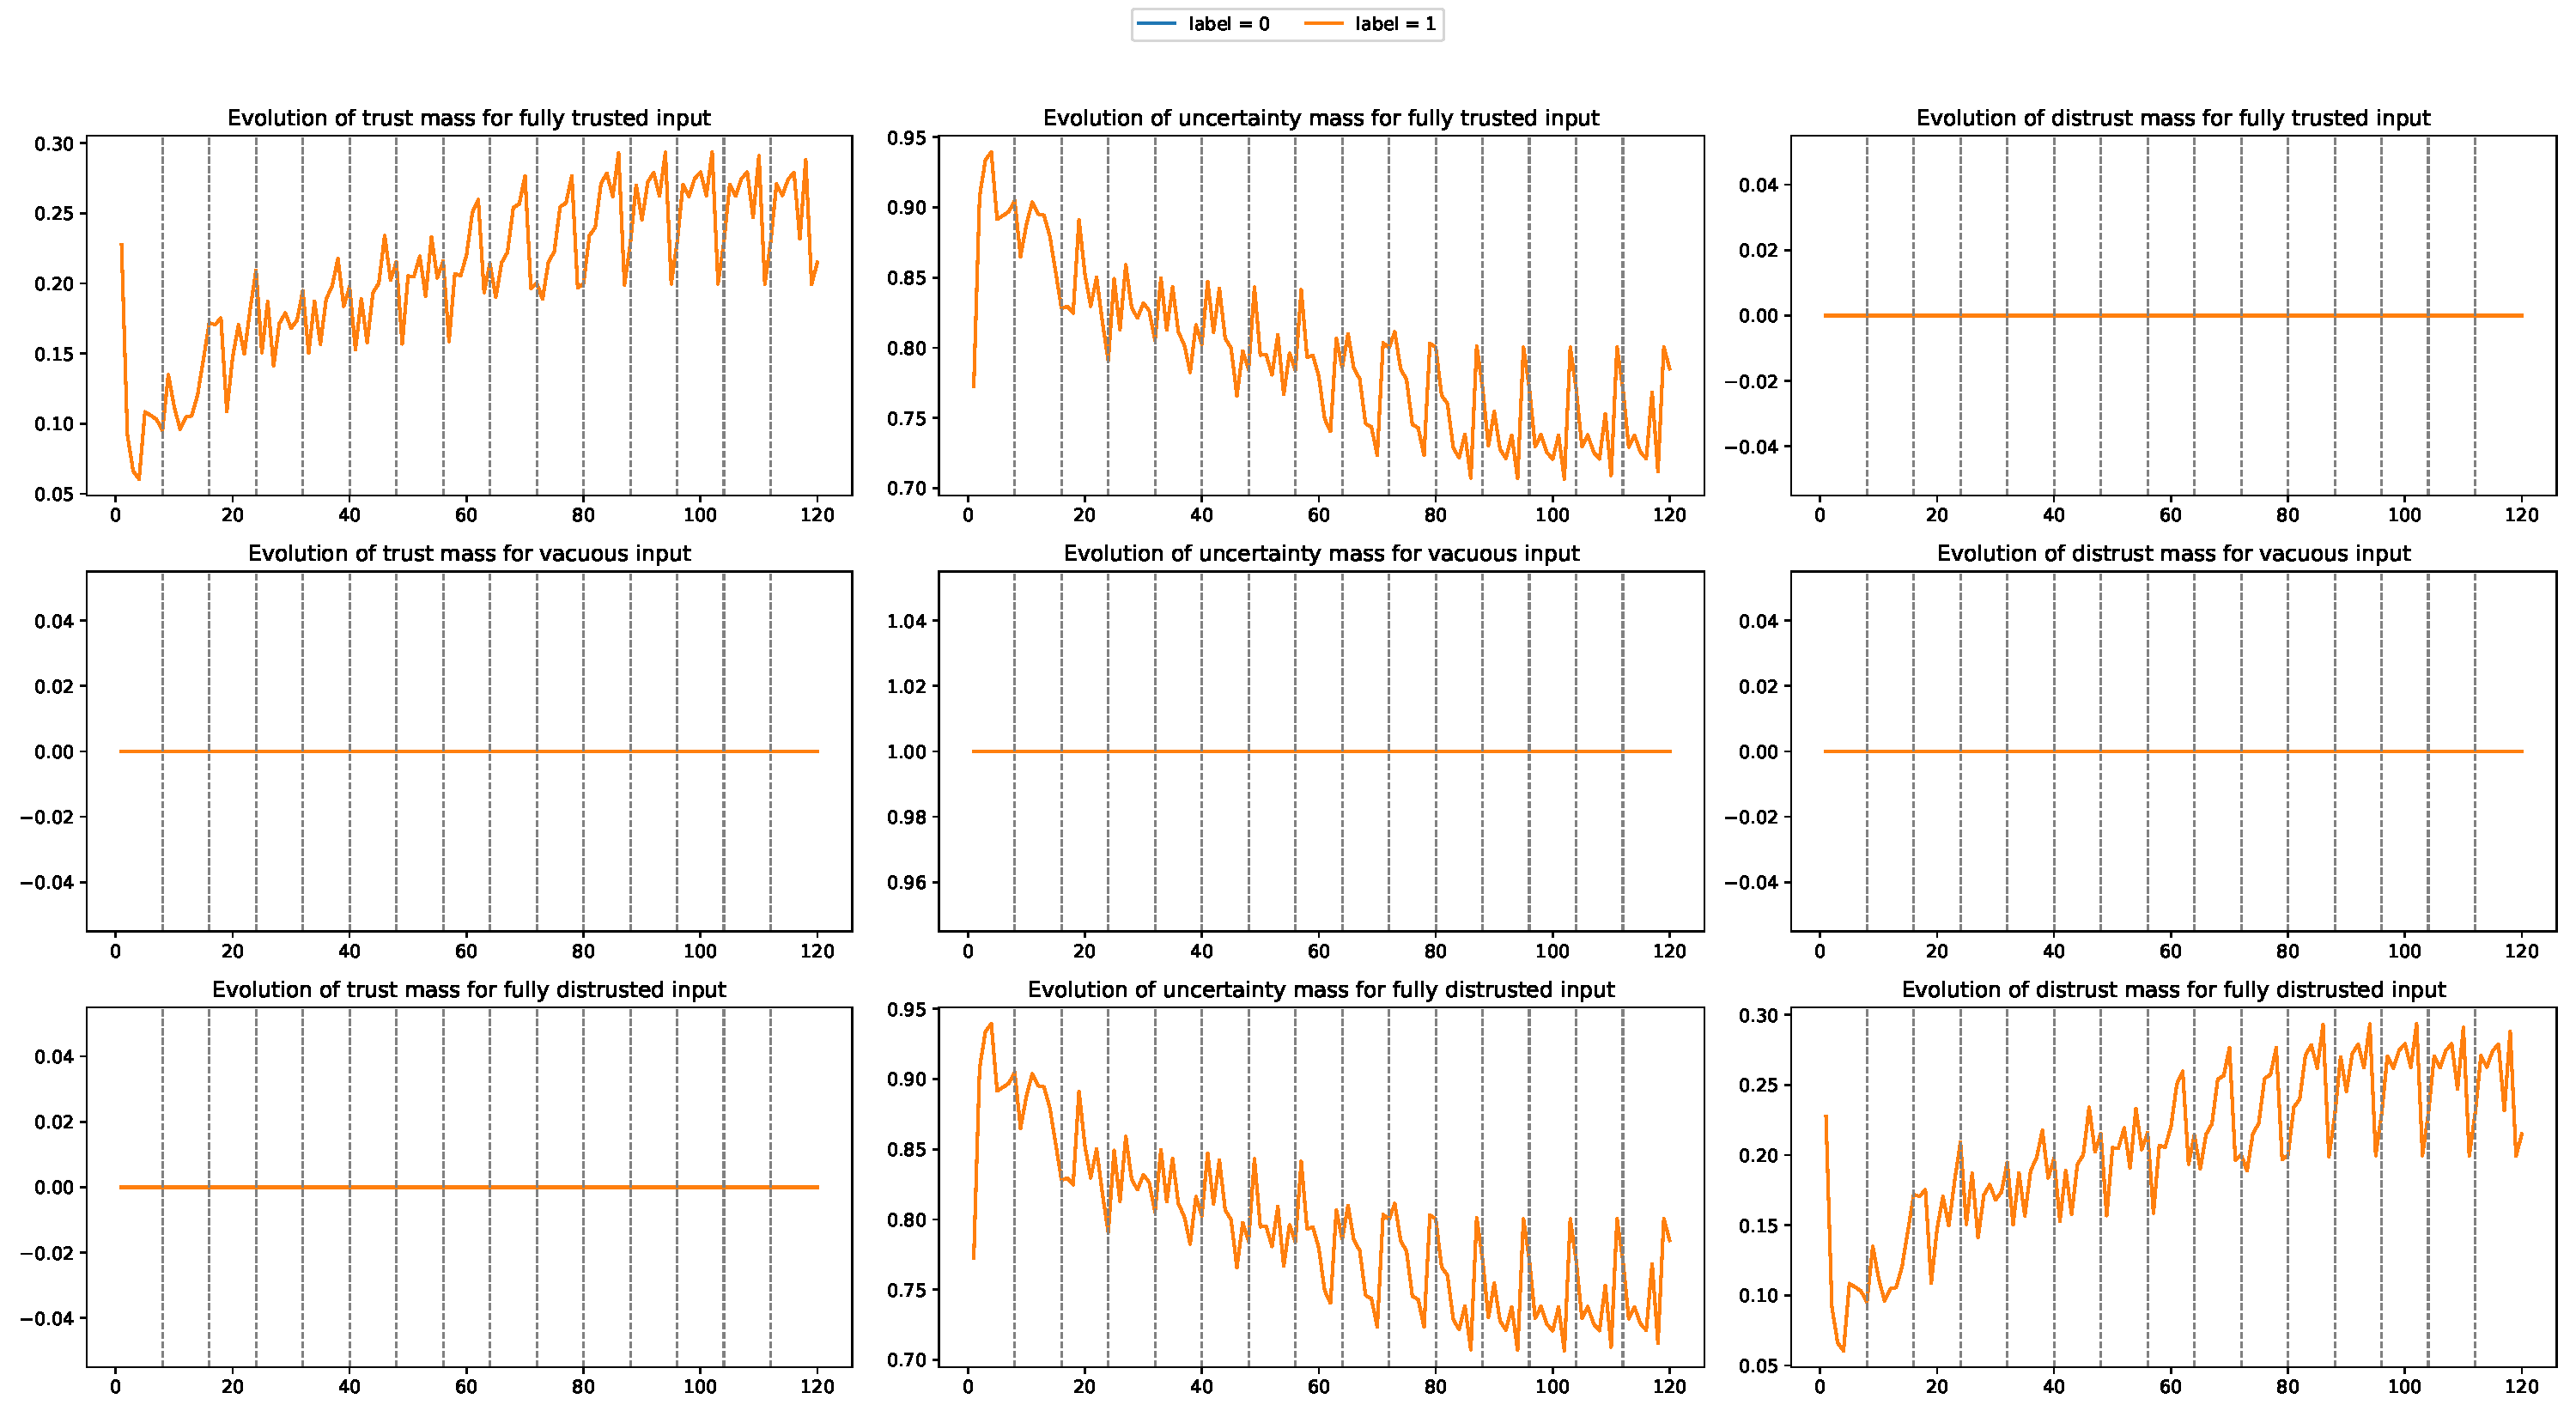
\includegraphics[width=0.8\textwidth]{latex/PTAS_Eval_cancer_16_vacuous_trust_eps_0.01_PathSize_None__plot_ptas.pdf}
\caption{cancer\_16\_vacuous\_trust, $\varepsilon$=0.01}
\end{figure}

\begin{figure}[htbp]
\centering
  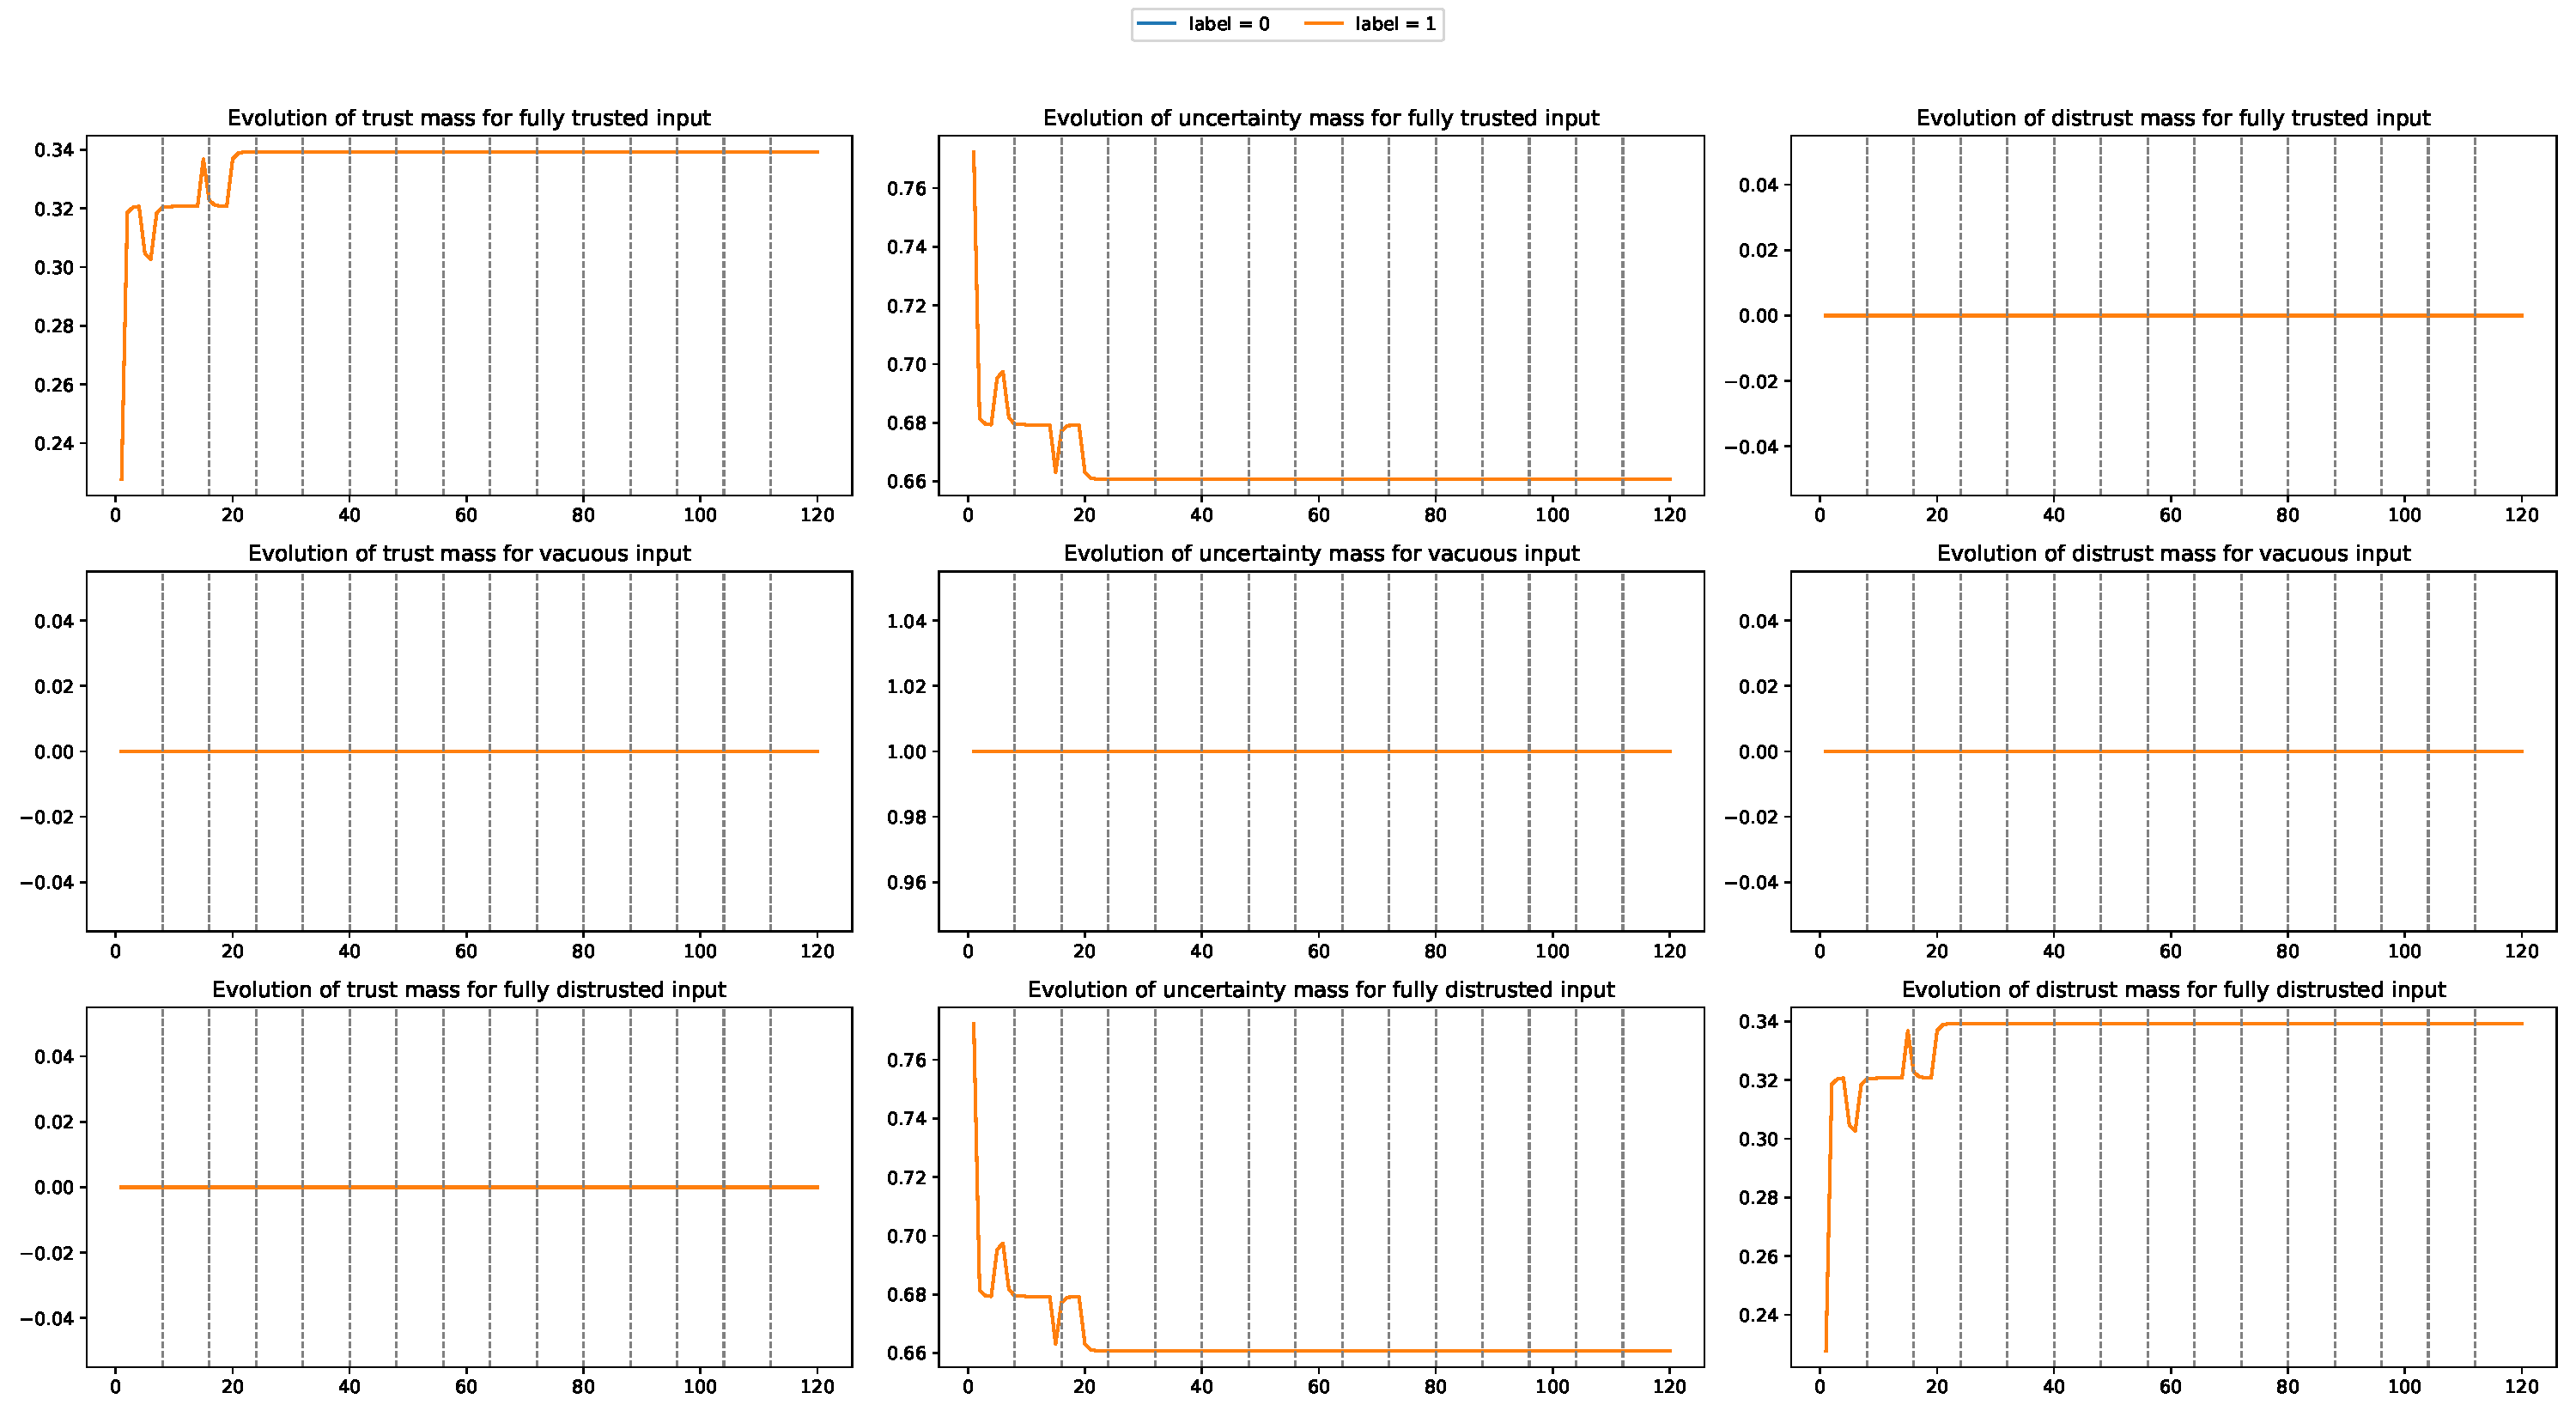
\includegraphics[width=0.8\textwidth]{latex/PTAS_Eval_cancer_16_vacuous_trust_eps_0.1_PathSize_None__plot_ptas.pdf}
\caption{cancer\_16\_vacuous\_trust, $\varepsilon$=0.1}
\end{figure}

\begin{figure}[htbp]
\centering
  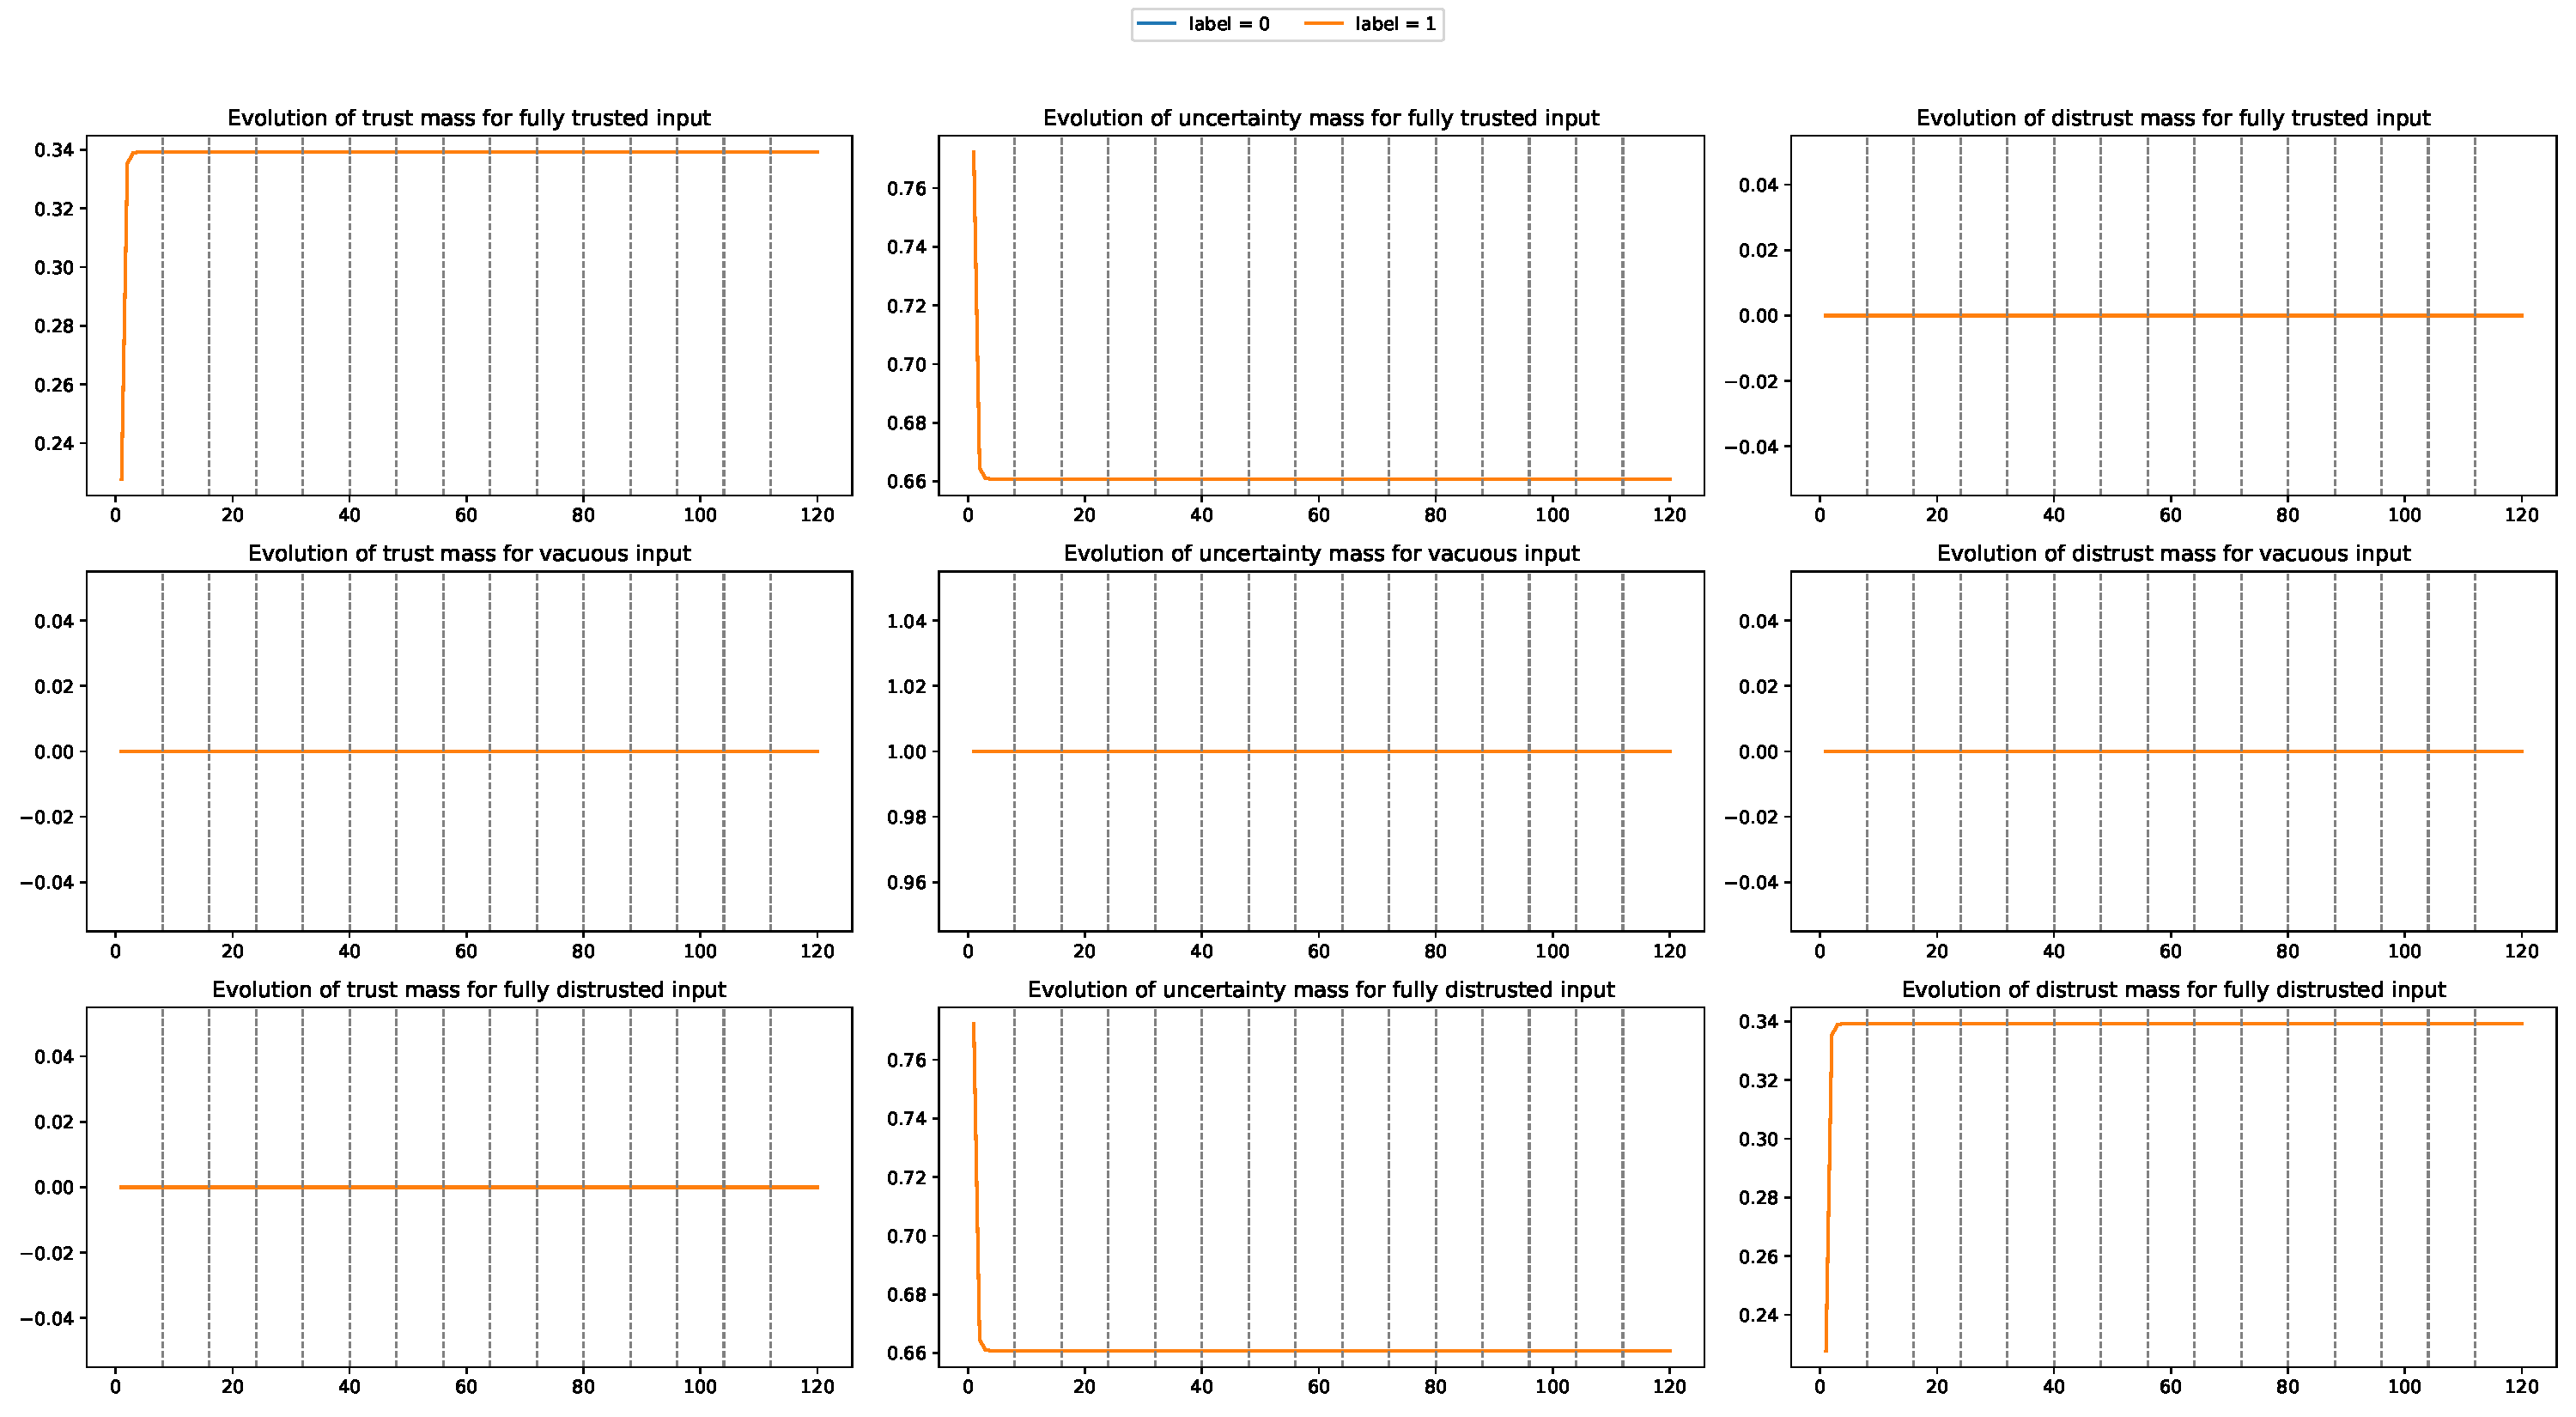
\includegraphics[width=0.8\textwidth]{latex/PTAS_Eval_cancer_16_vacuous_trust_eps_1_PathSize_None__plot_ptas.pdf}
\caption{cancer\_16\_vacuous\_trust, $\varepsilon$=1}
\end{figure}

\subsubsection{vacuous -- vacuous}

\begin{figure}[htbp]
\centering
  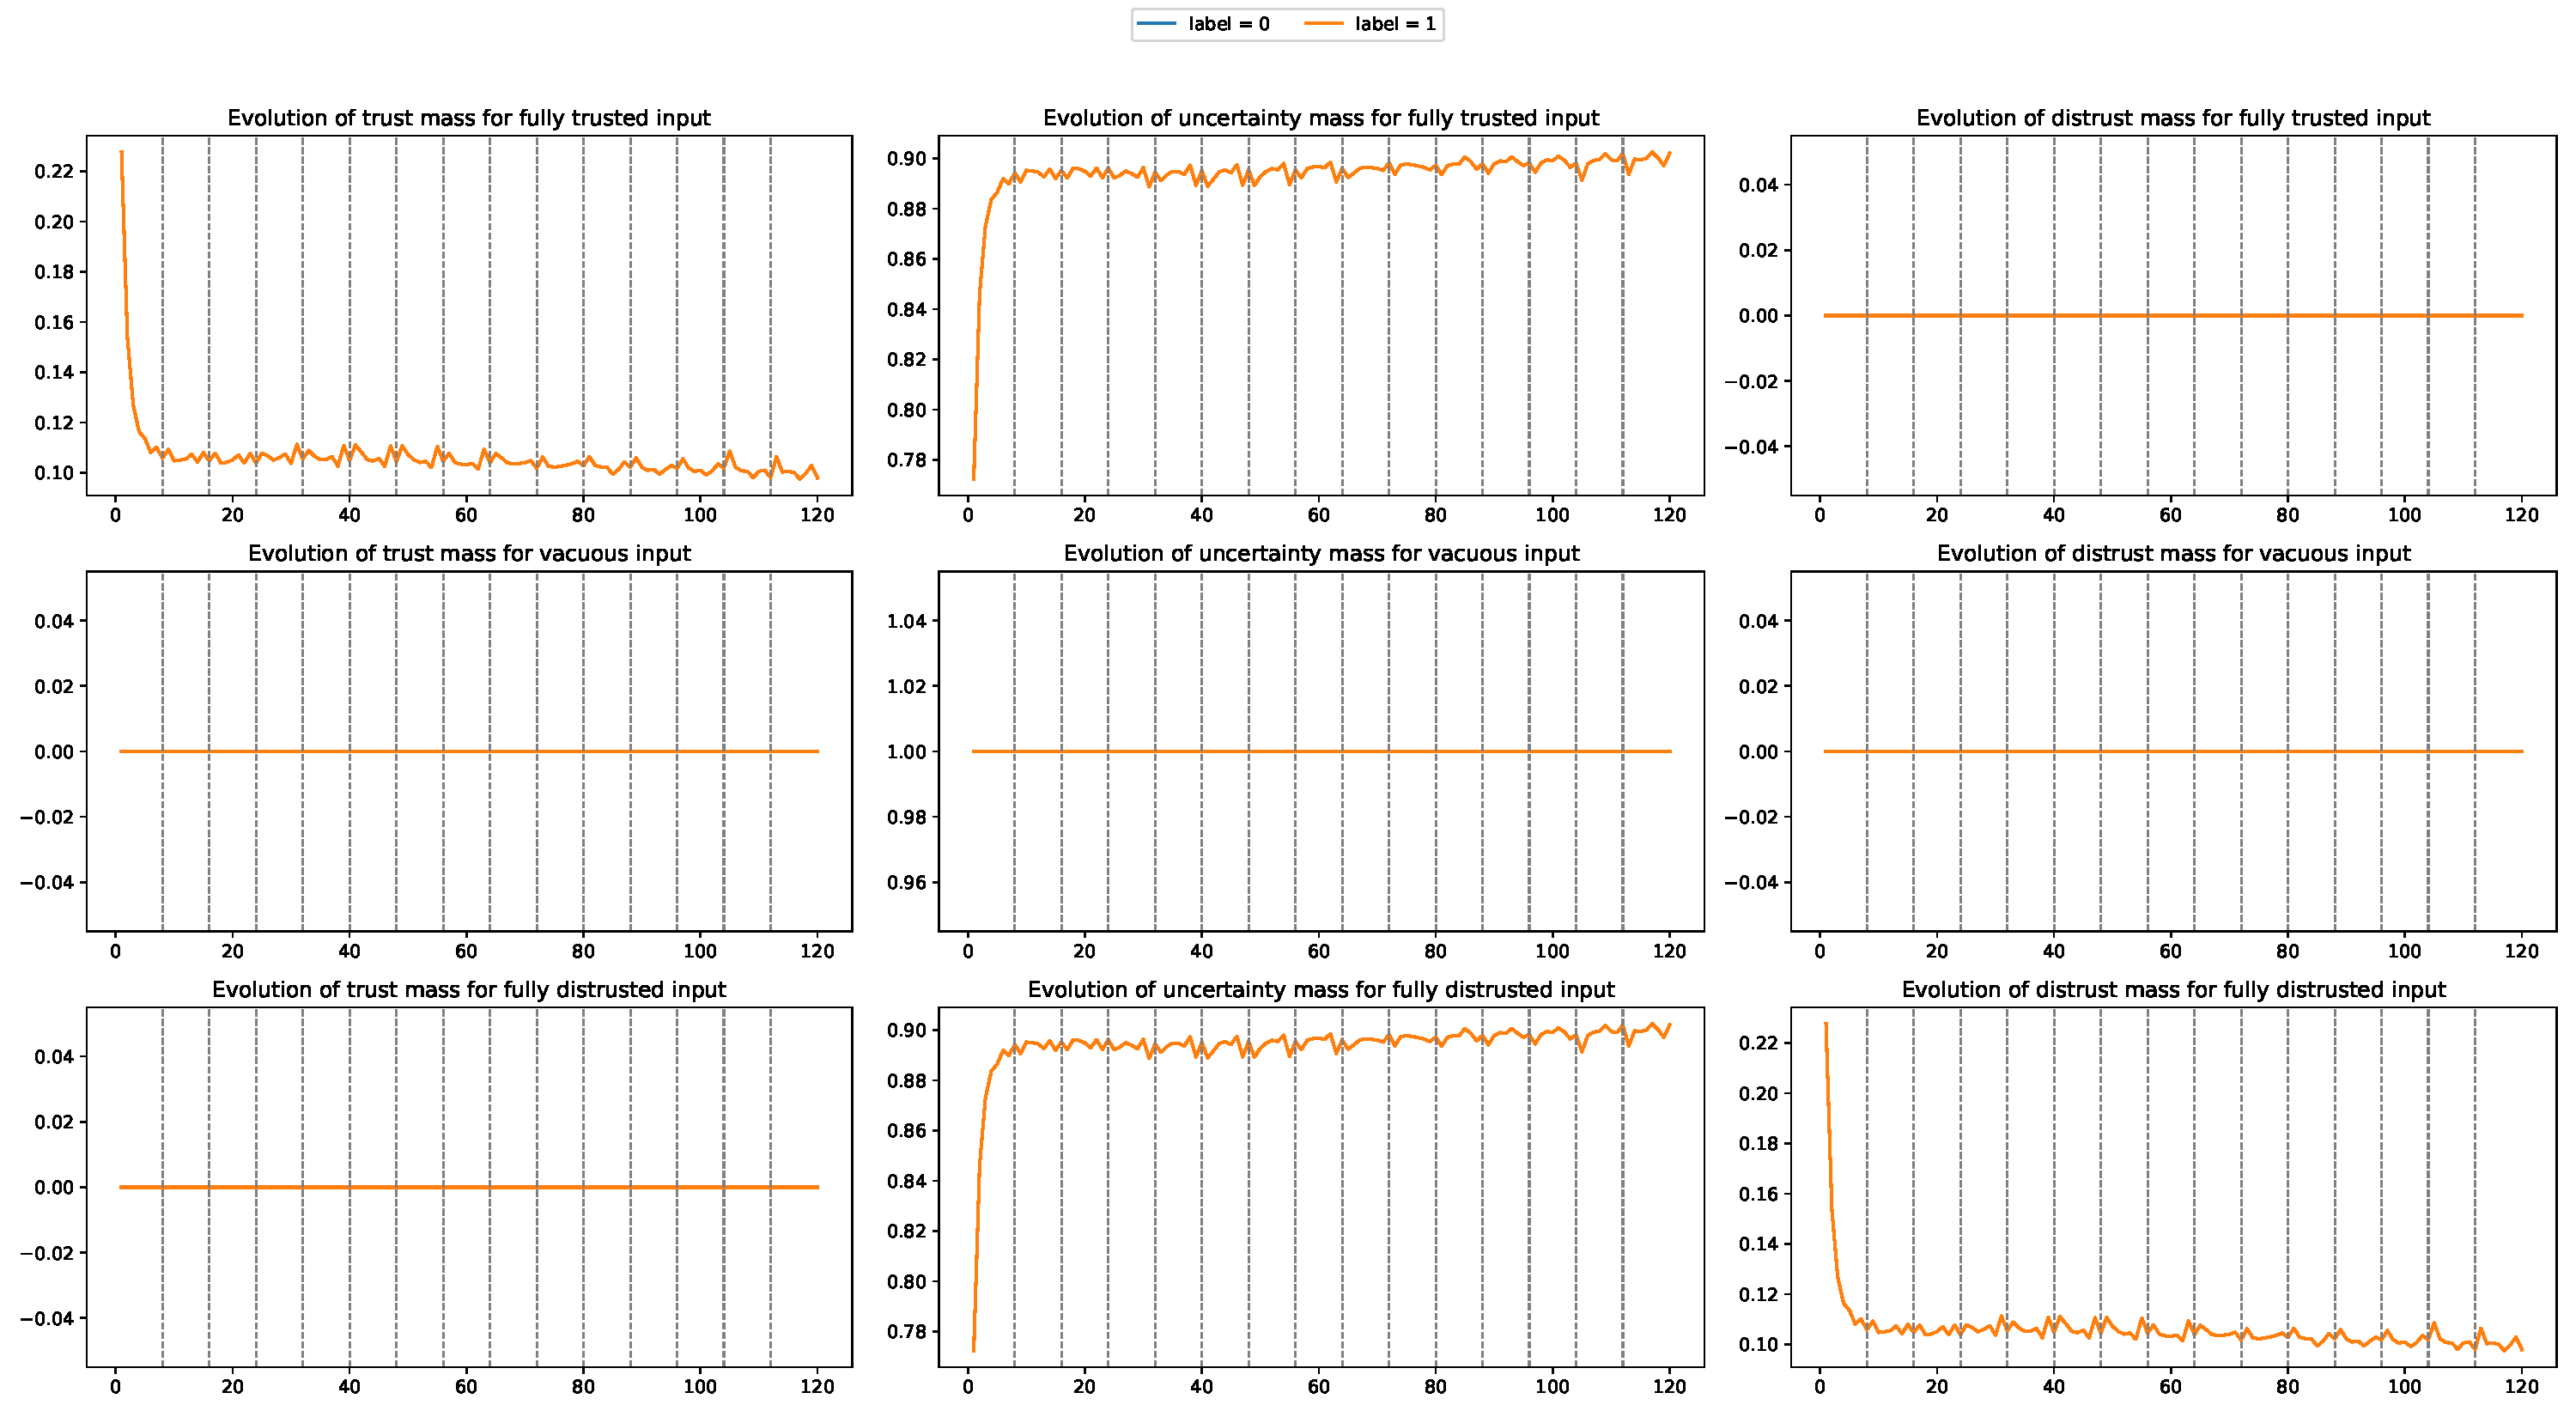
\includegraphics[width=0.8\textwidth]{latex/PTAS_Eval_cancer_16_vacuous_vacuous_eps_0.001_PathSize_None__plot_ptas.pdf}
\caption{cancer\_16\_vacuous\_vacuous, $\varepsilon$=0.001}
\end{figure}

\begin{figure}[htbp]
\centering
  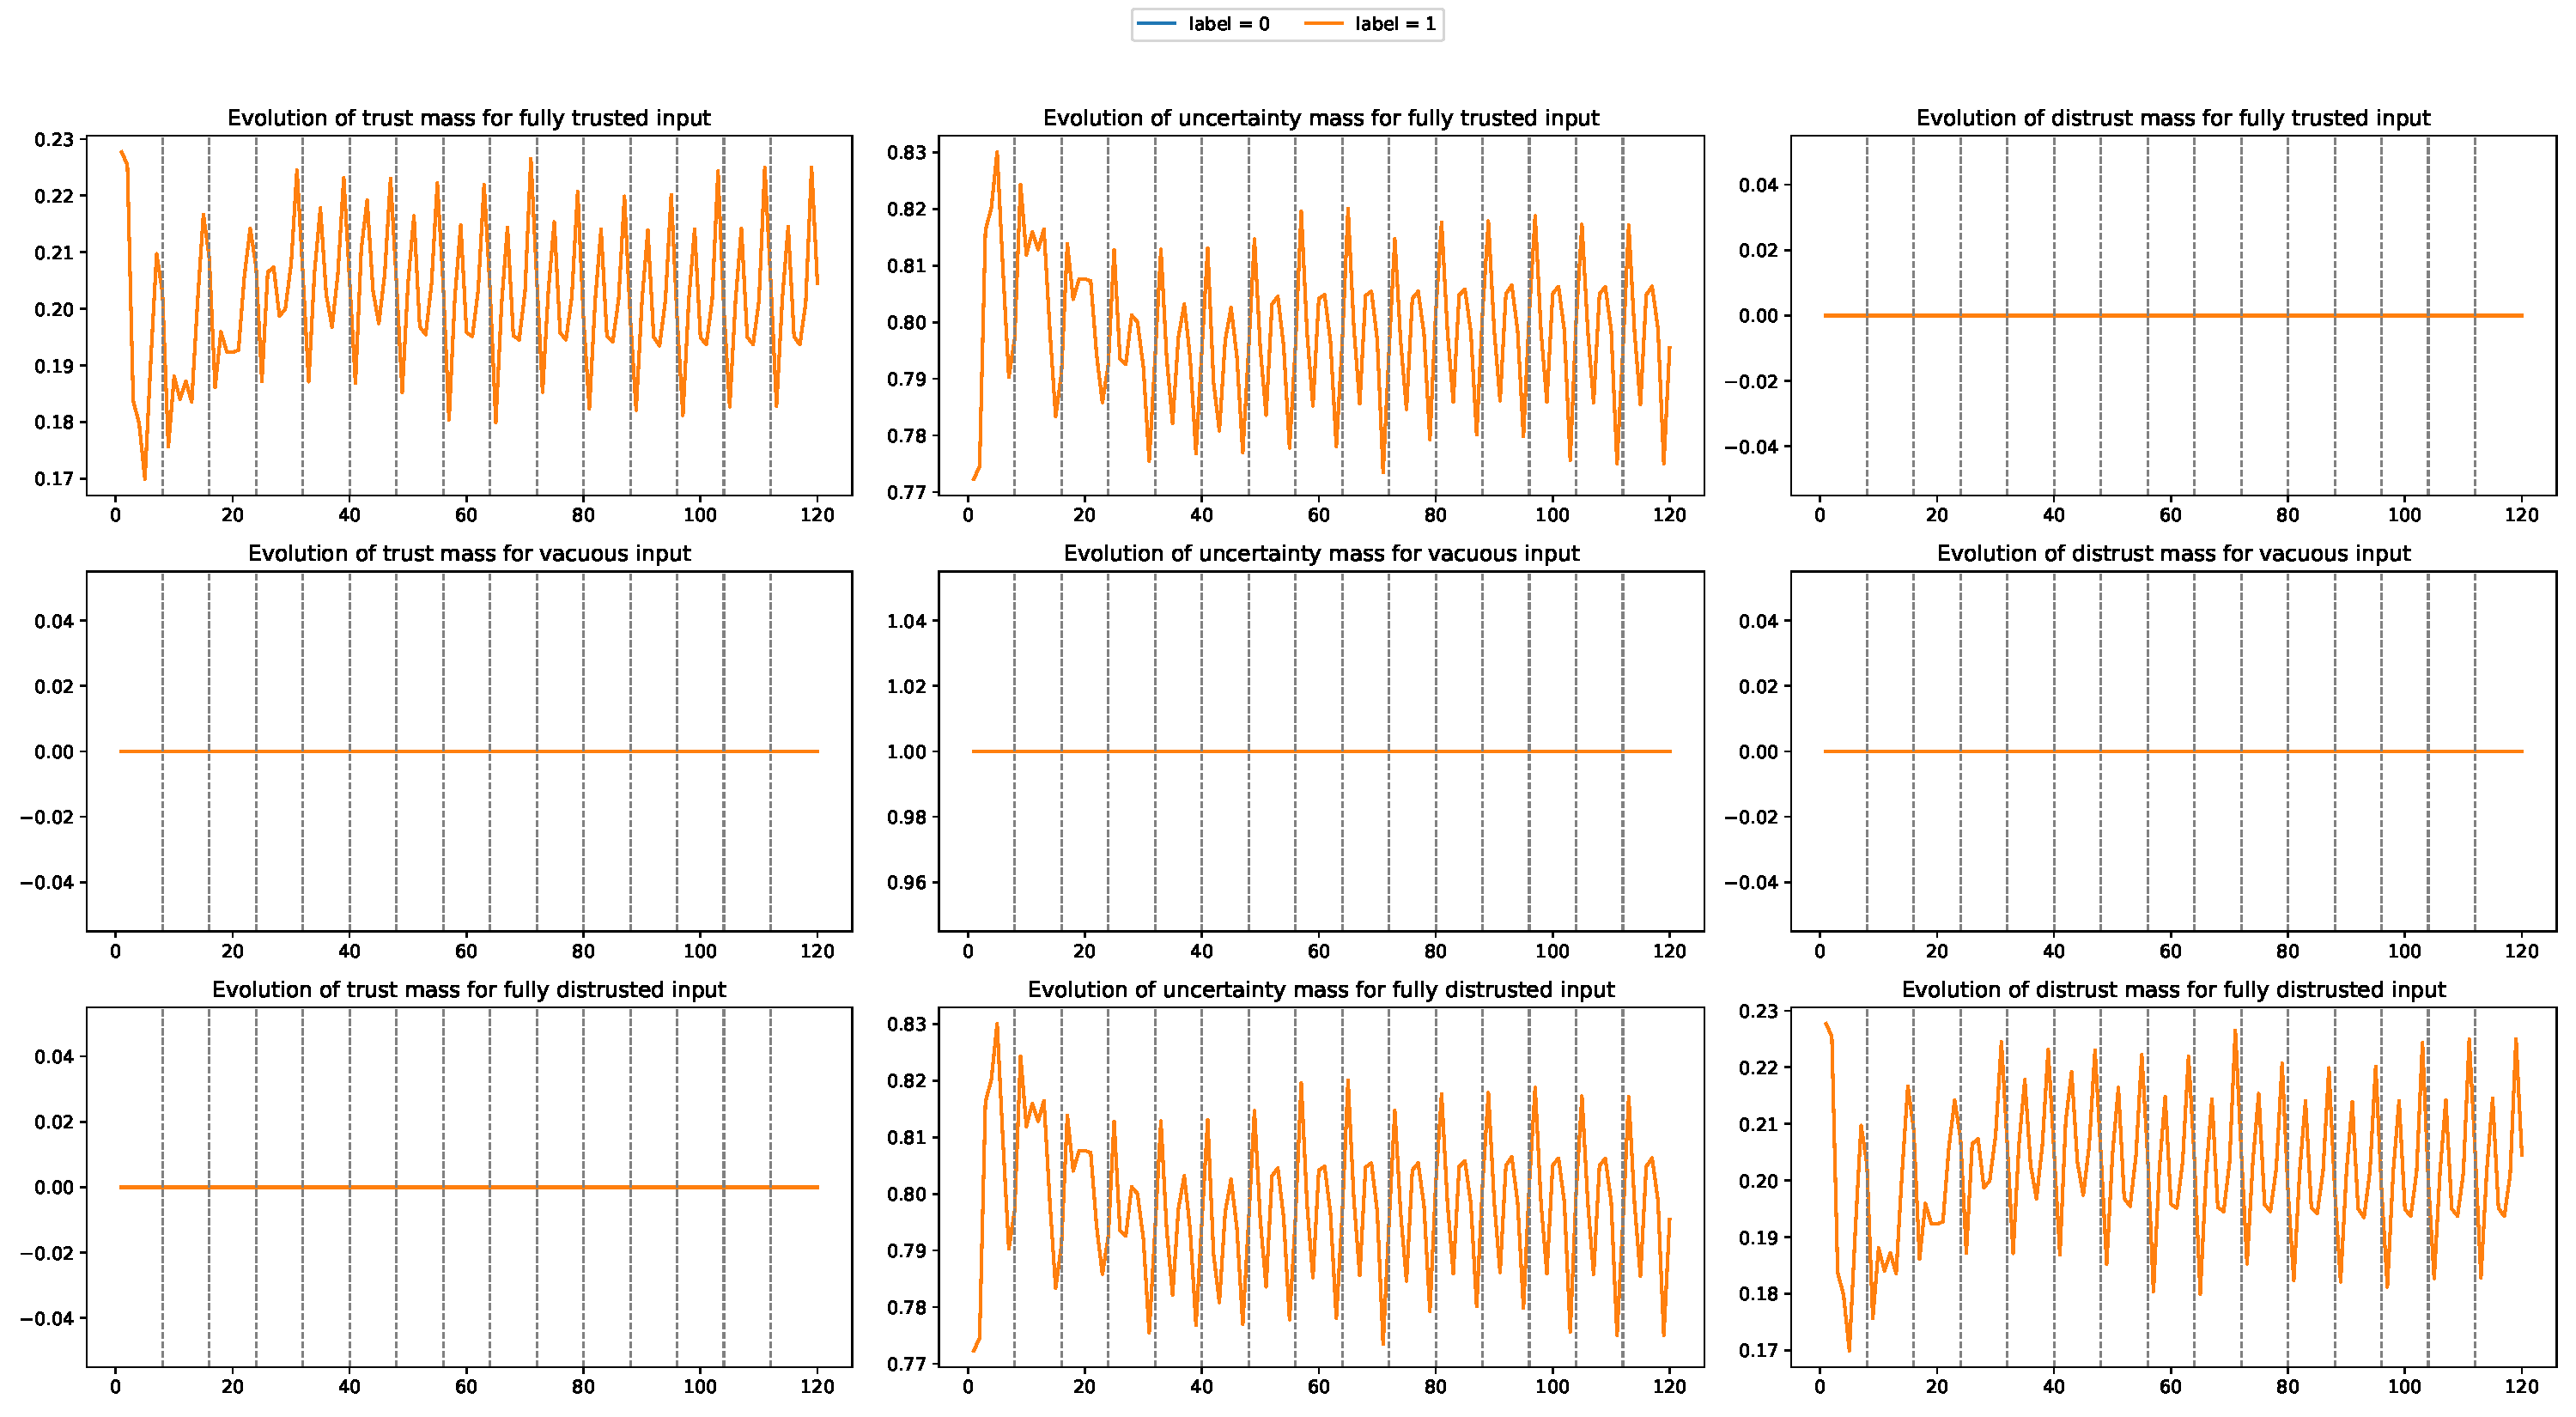
\includegraphics[width=0.8\textwidth]{latex/PTAS_Eval_cancer_16_vacuous_vacuous_eps_0.01_PathSize_None__plot_ptas.pdf}
\caption{cancer\_16\_vacuous\_vacuous, $\varepsilon$=0.01}
\end{figure}

\begin{figure}[htbp]
\centering
  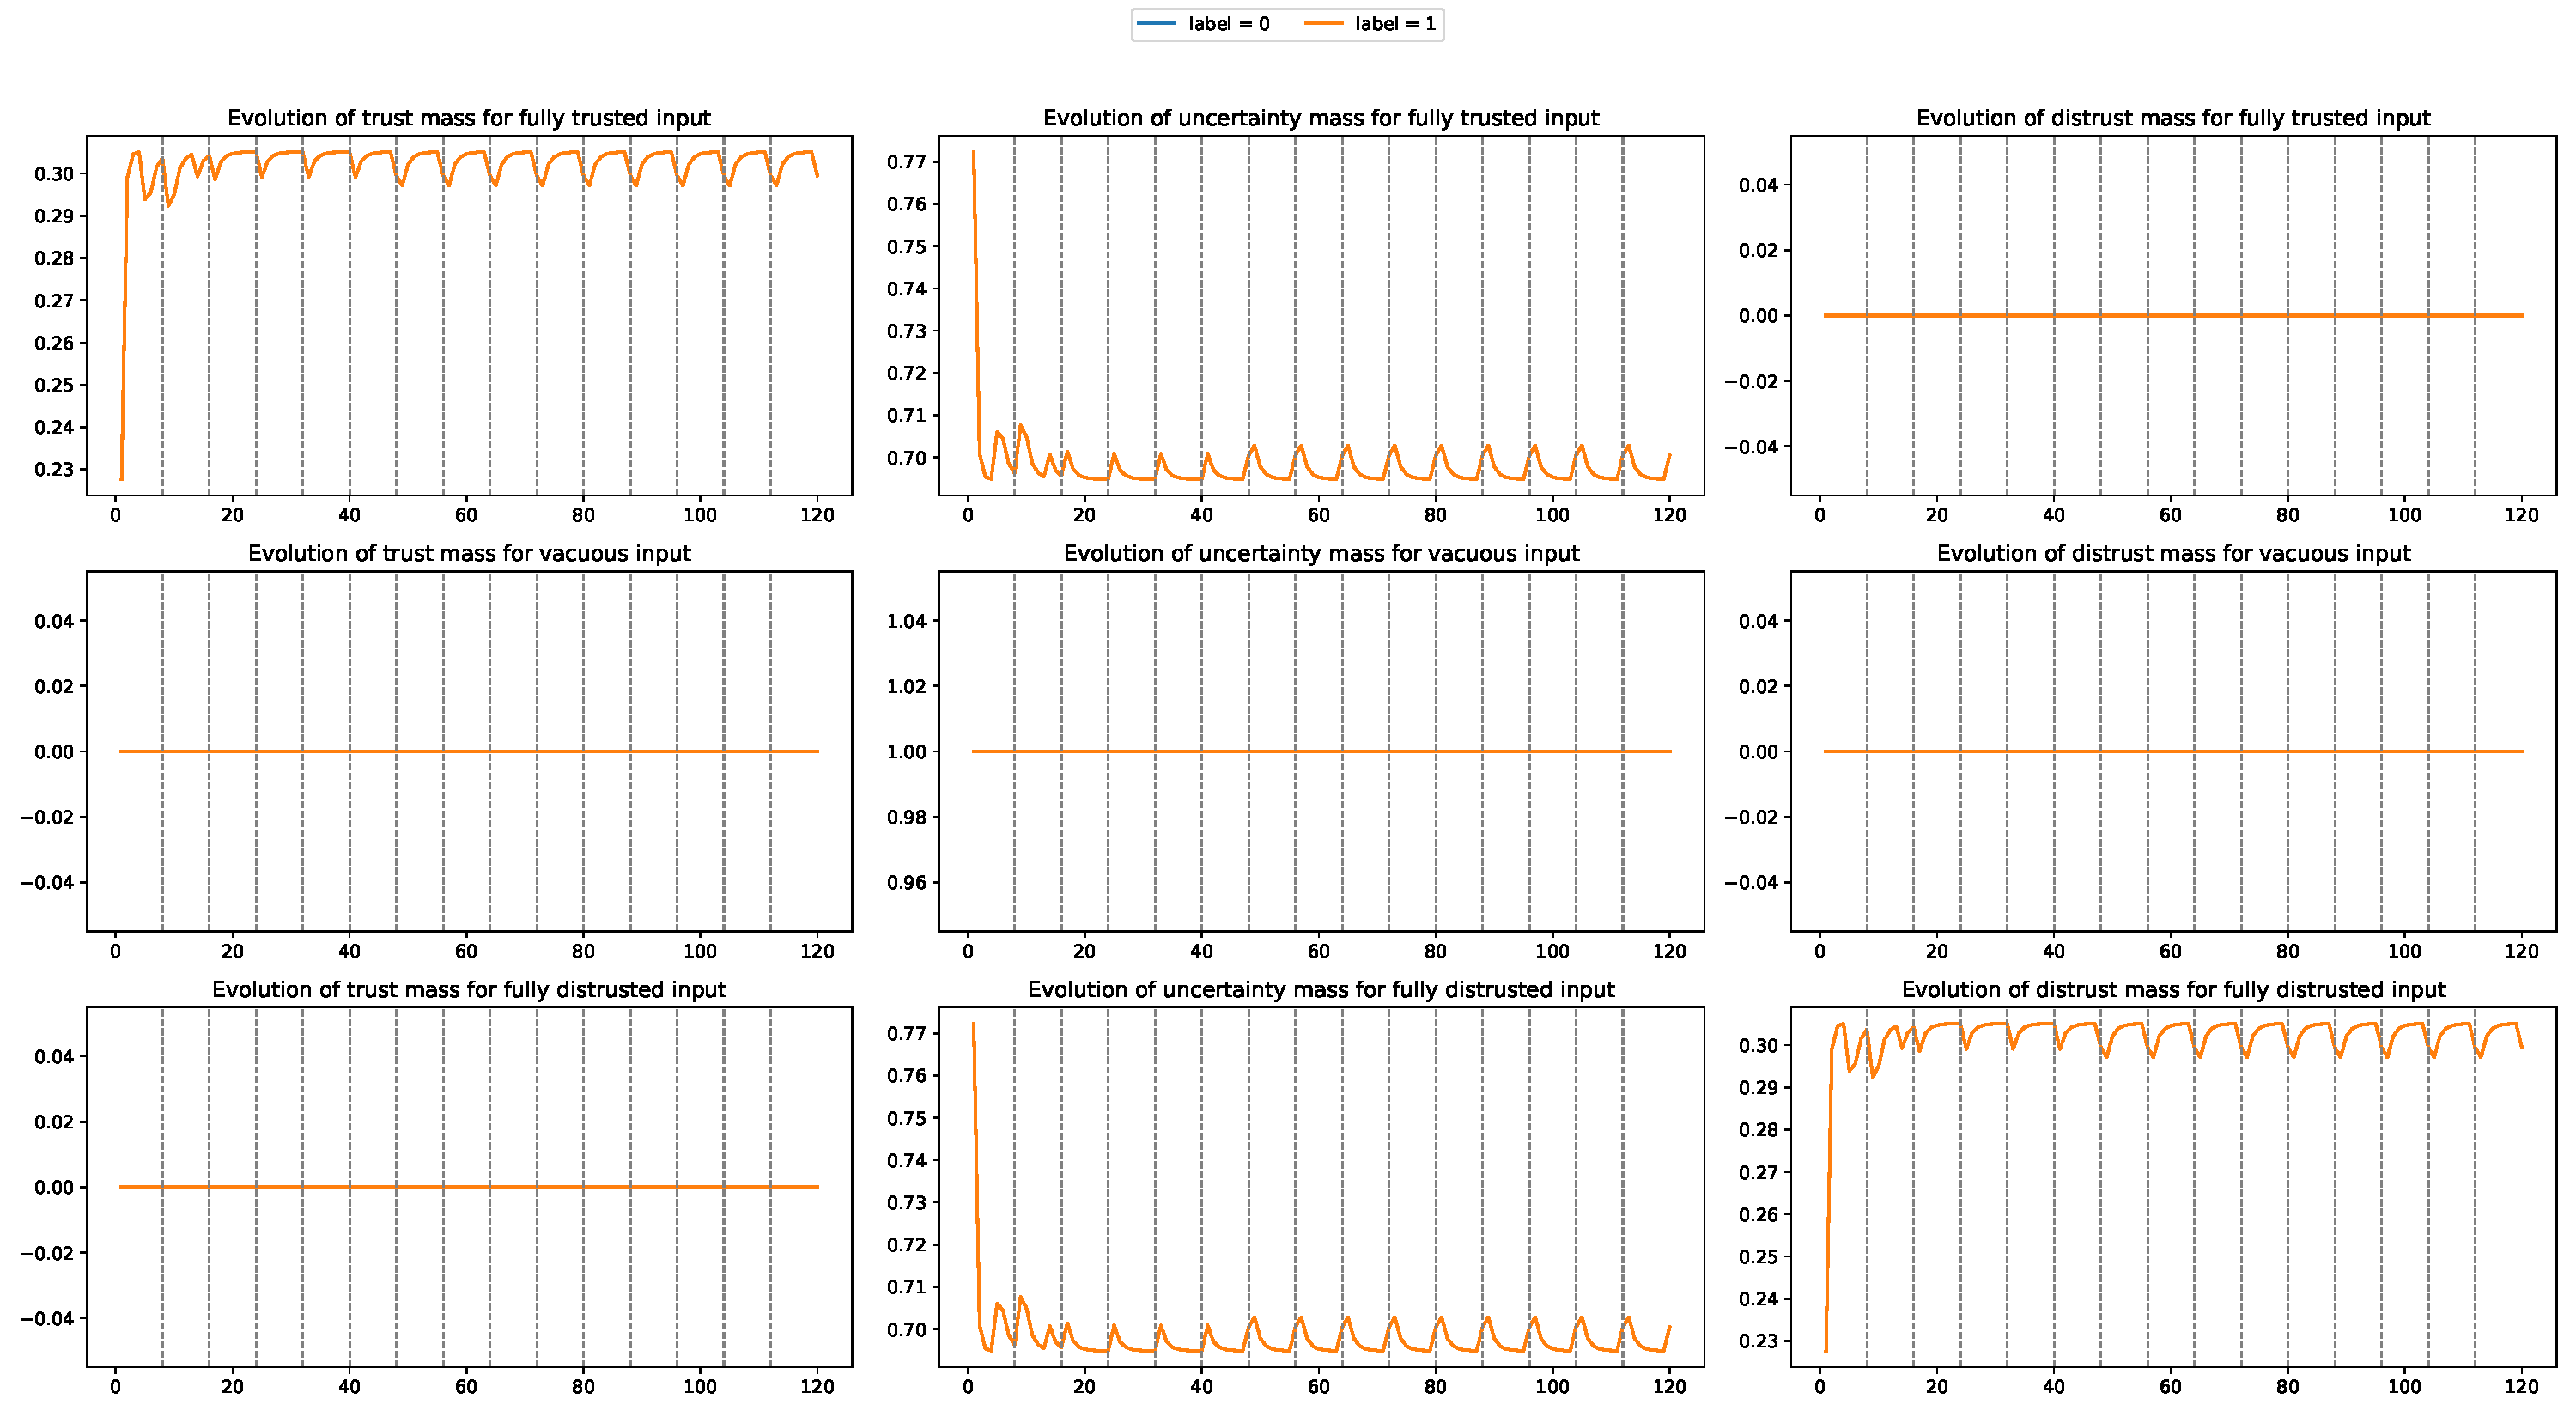
\includegraphics[width=0.8\textwidth]{latex/PTAS_Eval_cancer_16_vacuous_vacuous_eps_0.1_PathSize_None__plot_ptas.pdf}
\caption{cancer\_16\_vacuous\_vacuous, $\varepsilon$=0.1}
\end{figure}

\begin{figure}[htbp]
\centering
  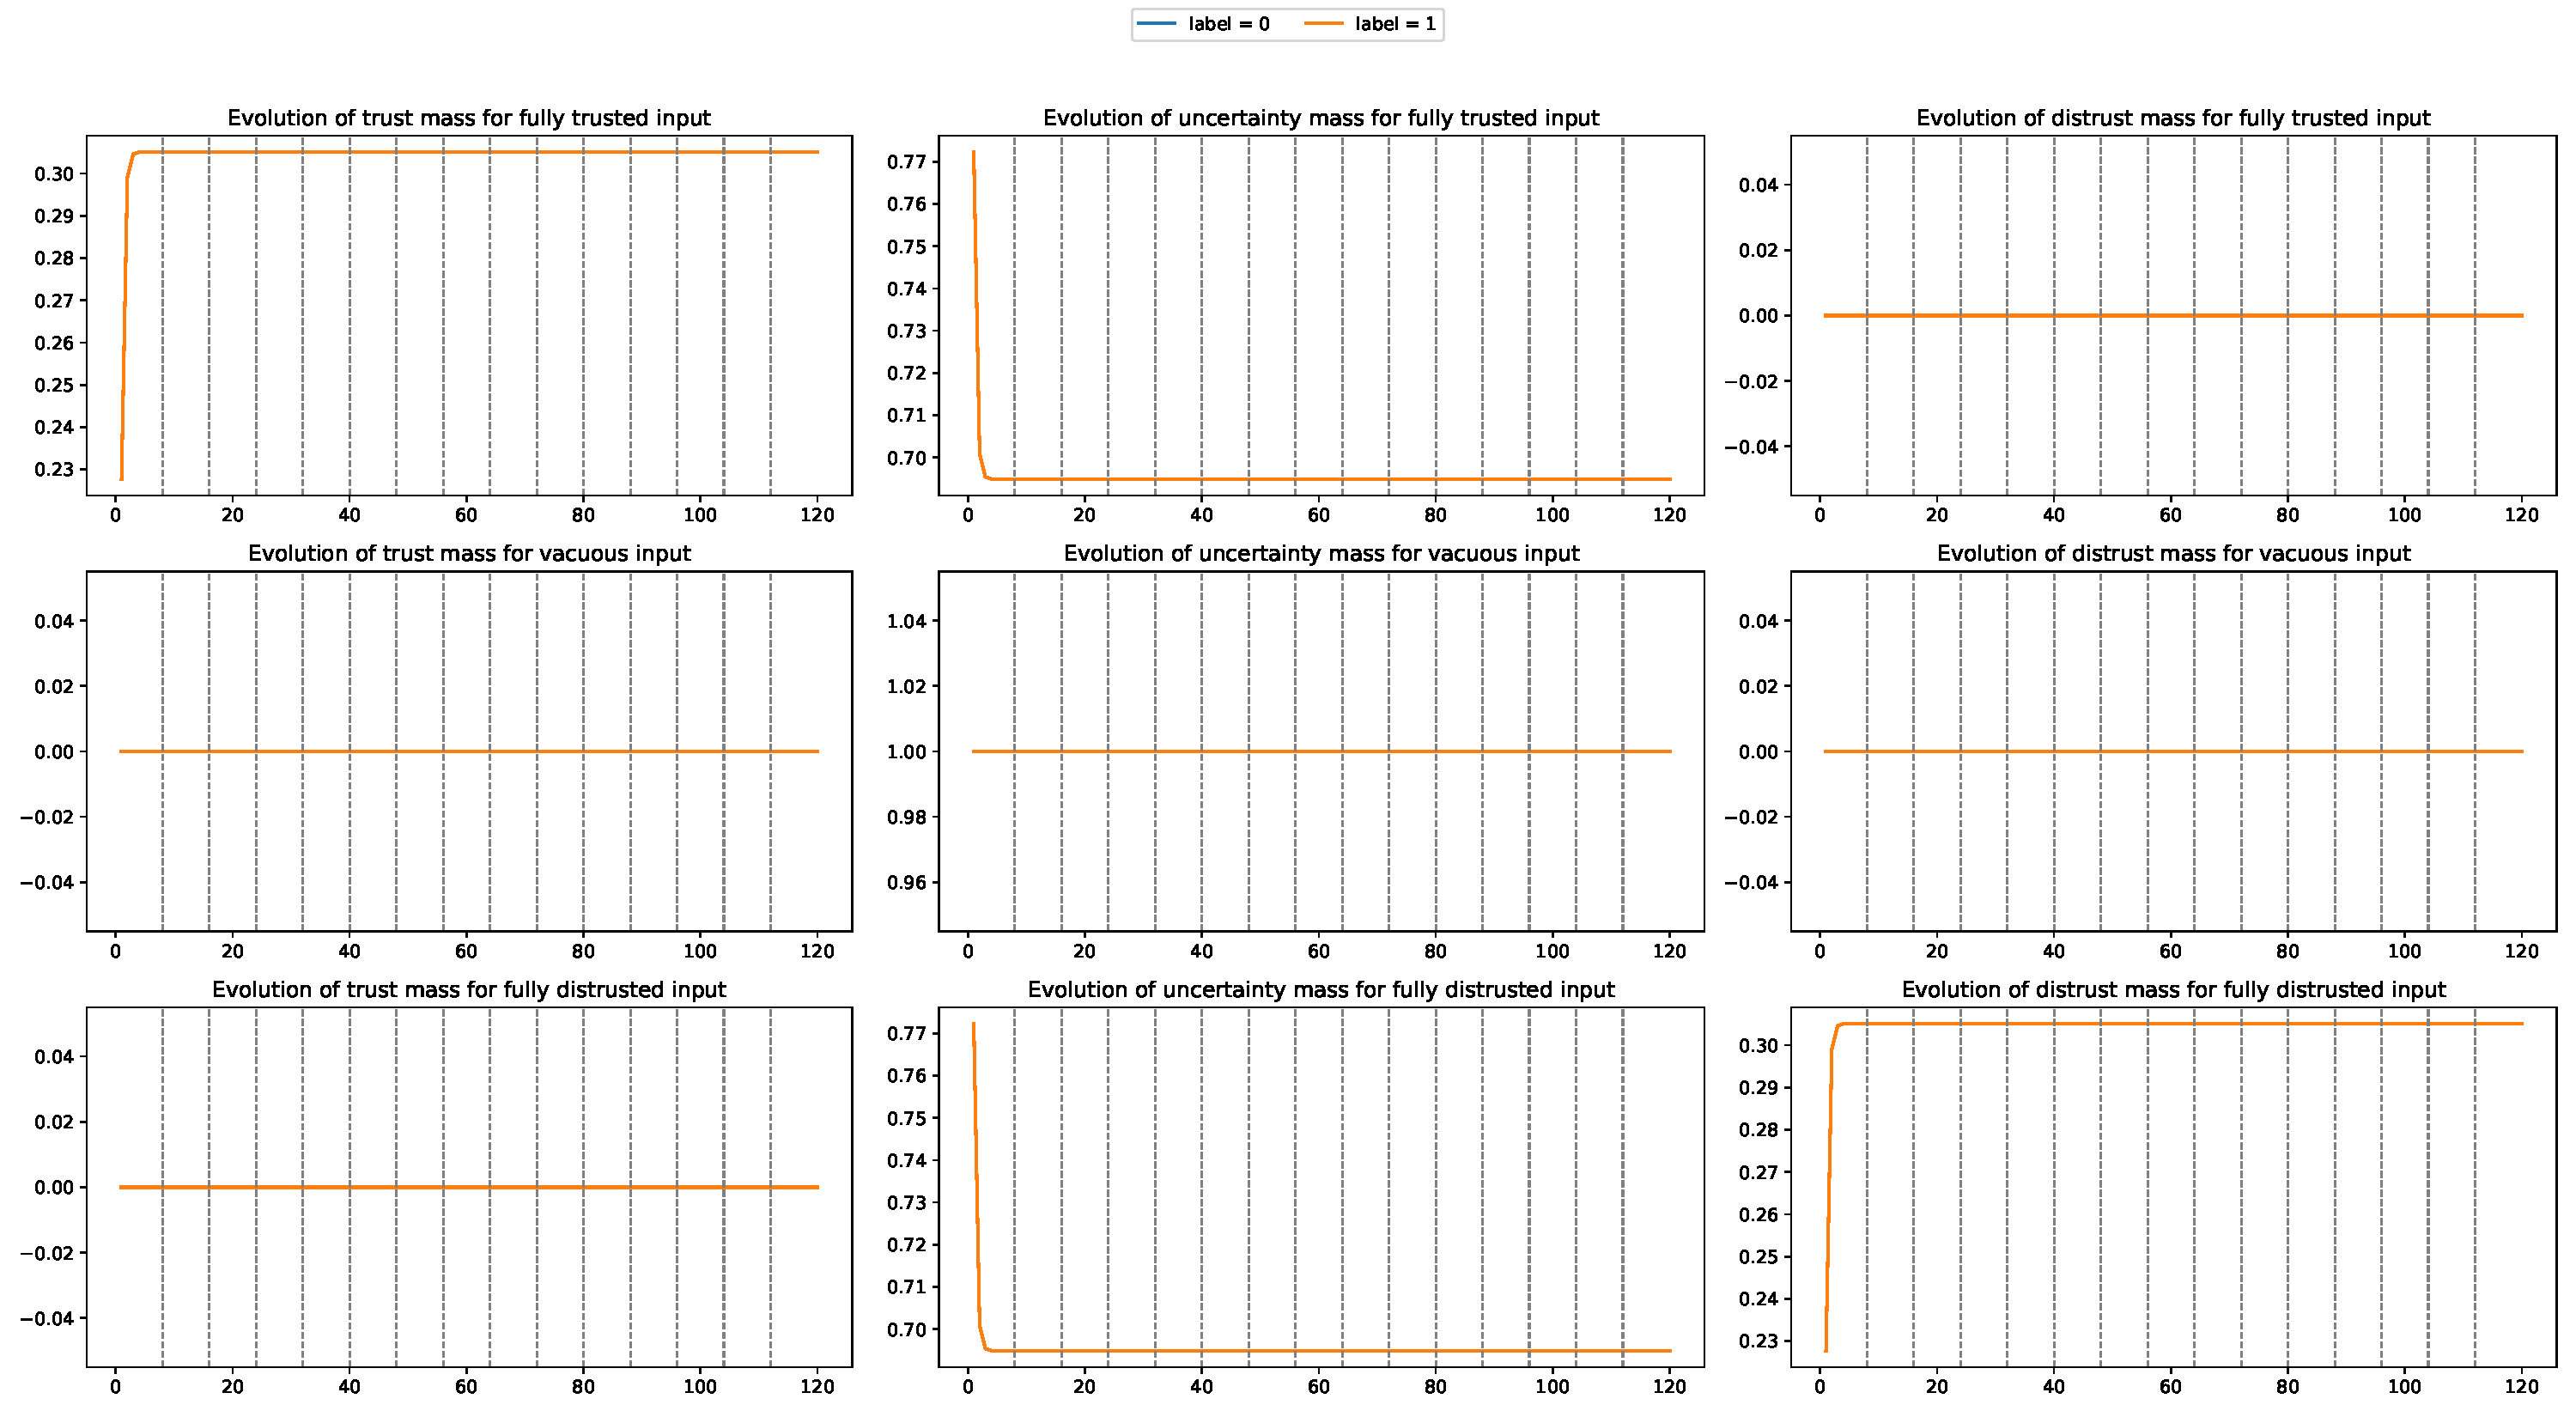
\includegraphics[width=0.8\textwidth]{latex/PTAS_Eval_cancer_16_vacuous_vacuous_eps_1_PathSize_None__plot_ptas.pdf}
\caption{cancer\_16\_vacuous\_vacuous, $\varepsilon$=1}
\end{figure}

\subsection{MNIST Dataset}

\subsubsection{trust -- trust}

\begin{figure}[htbp]
\centering
  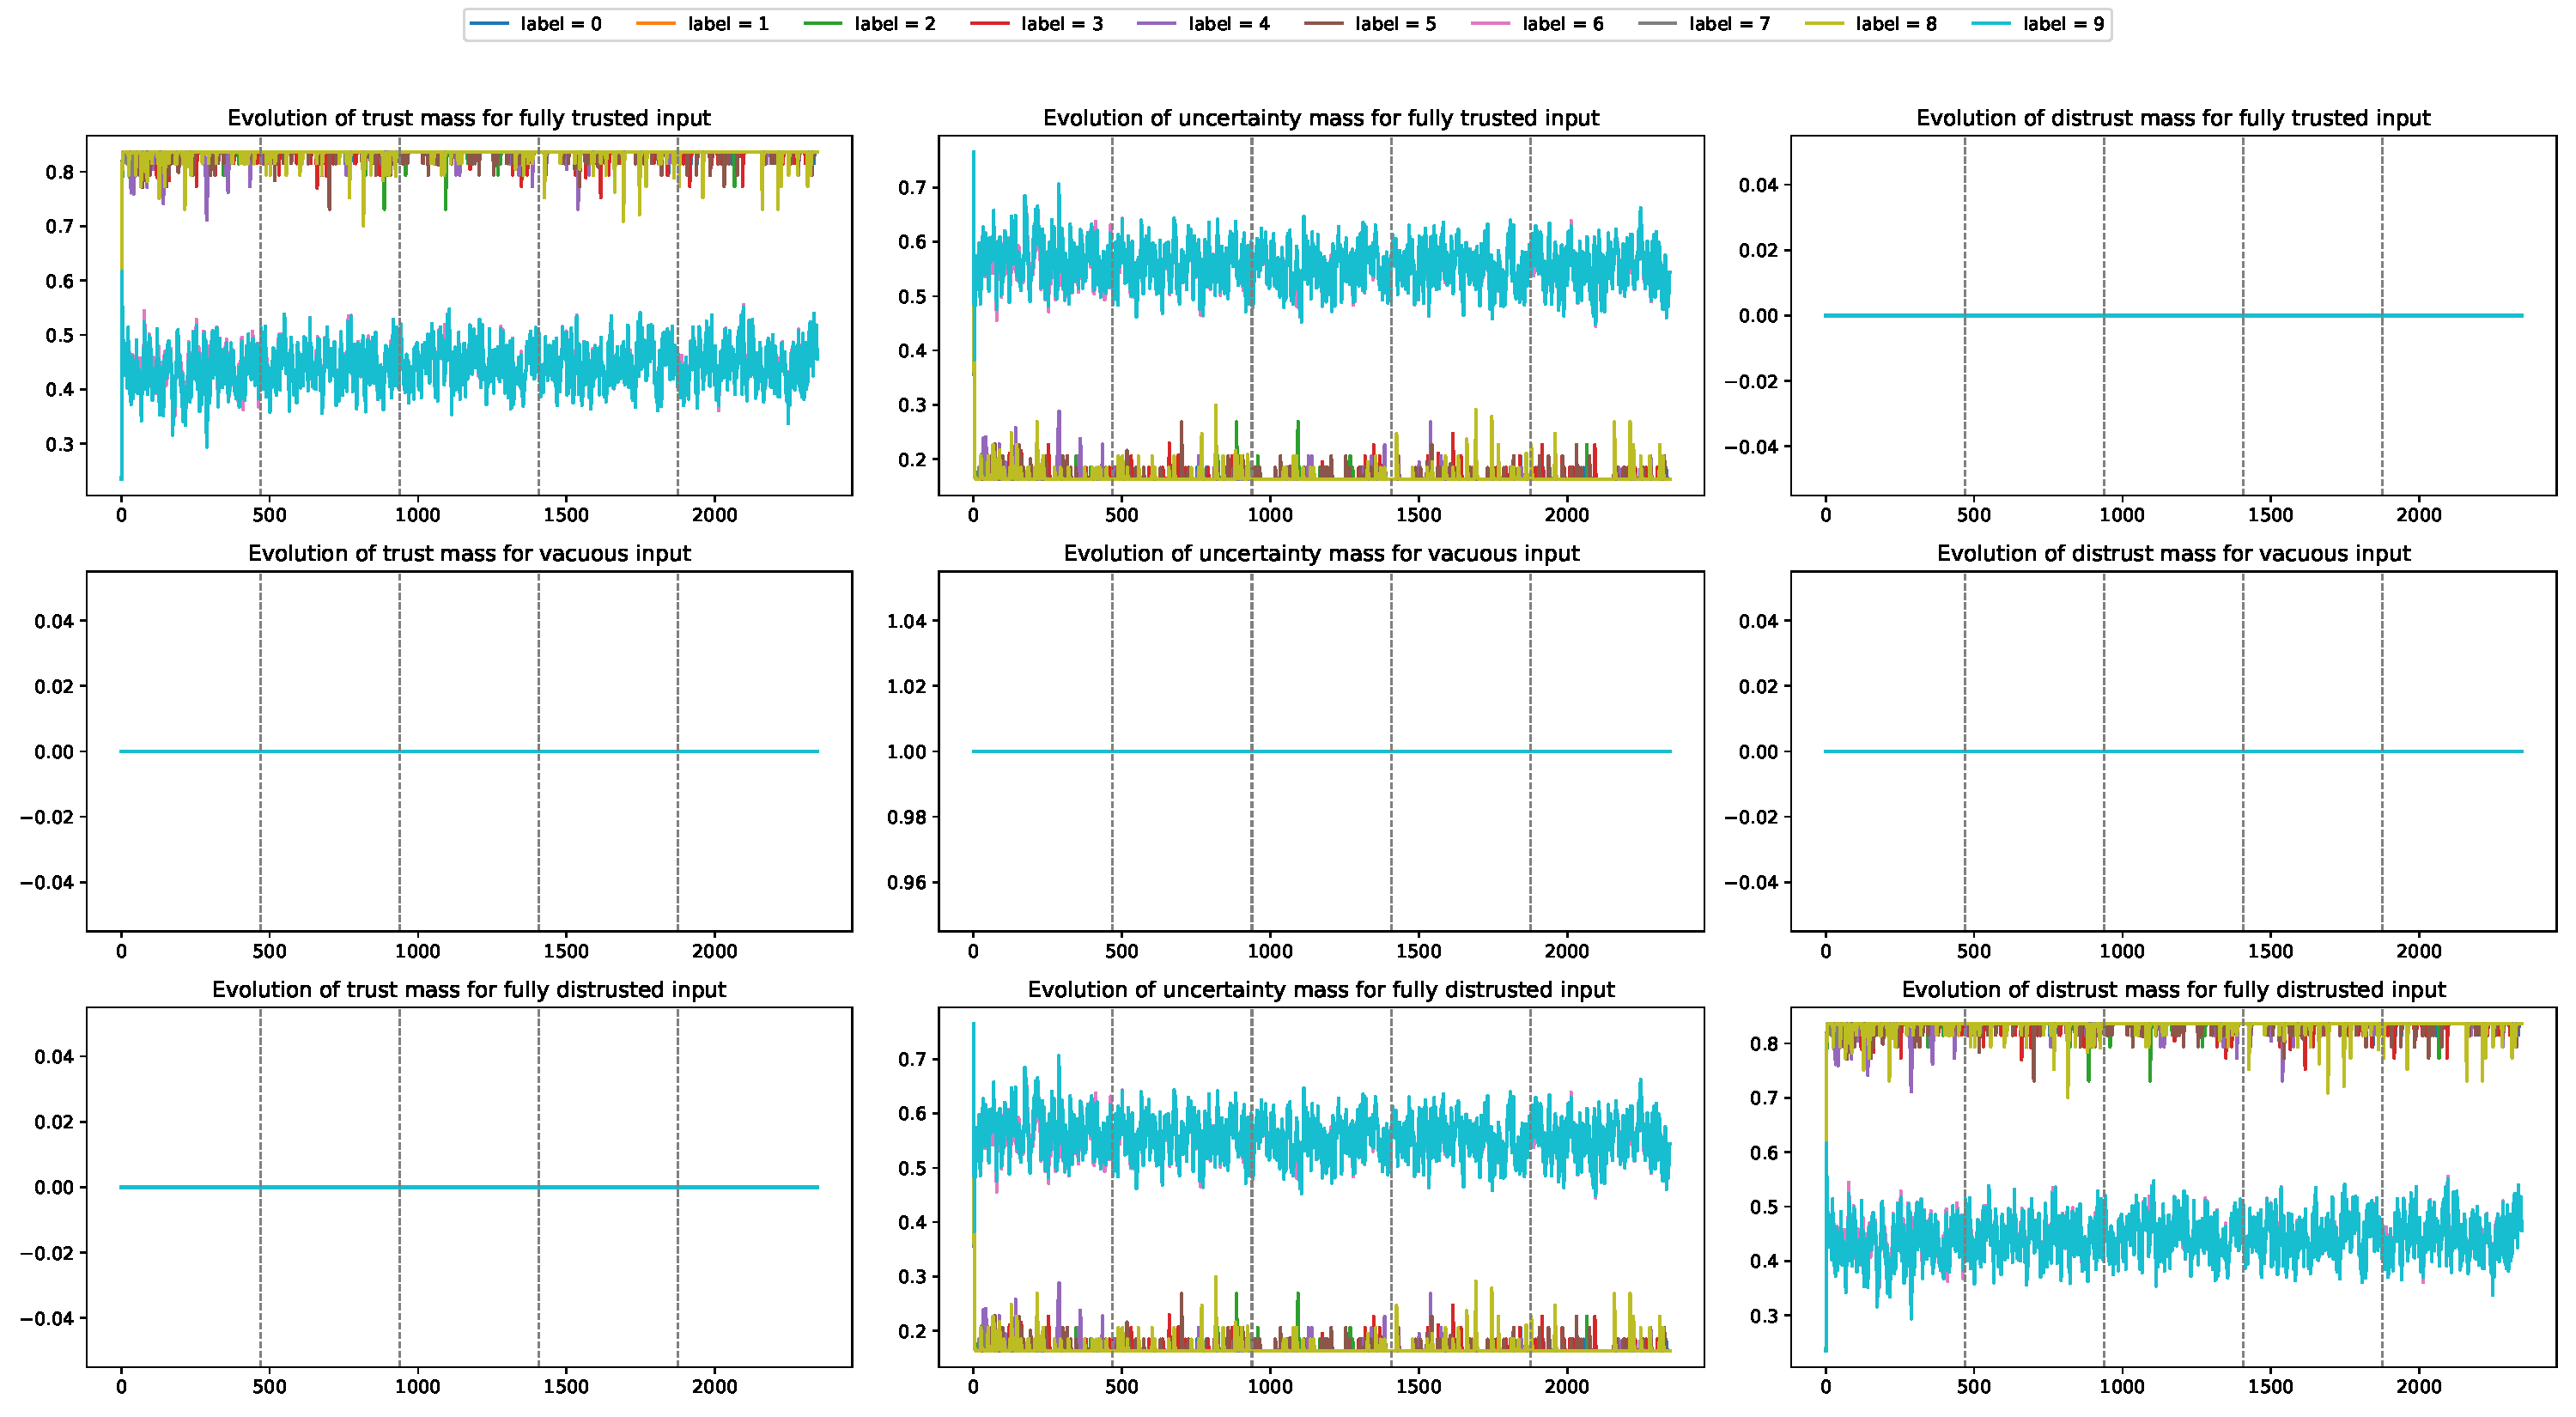
\includegraphics[width=0.8\textwidth]{latex/PTAS_Eval_mnist_128_trust_trust_eps_0.05_PathSize_1__plot_ptas.pdf}
\caption{mnist\_128\_trust\_trust, $\varepsilon$=0.05, ps=1}
\end{figure}

\begin{figure}[htbp]
\centering
  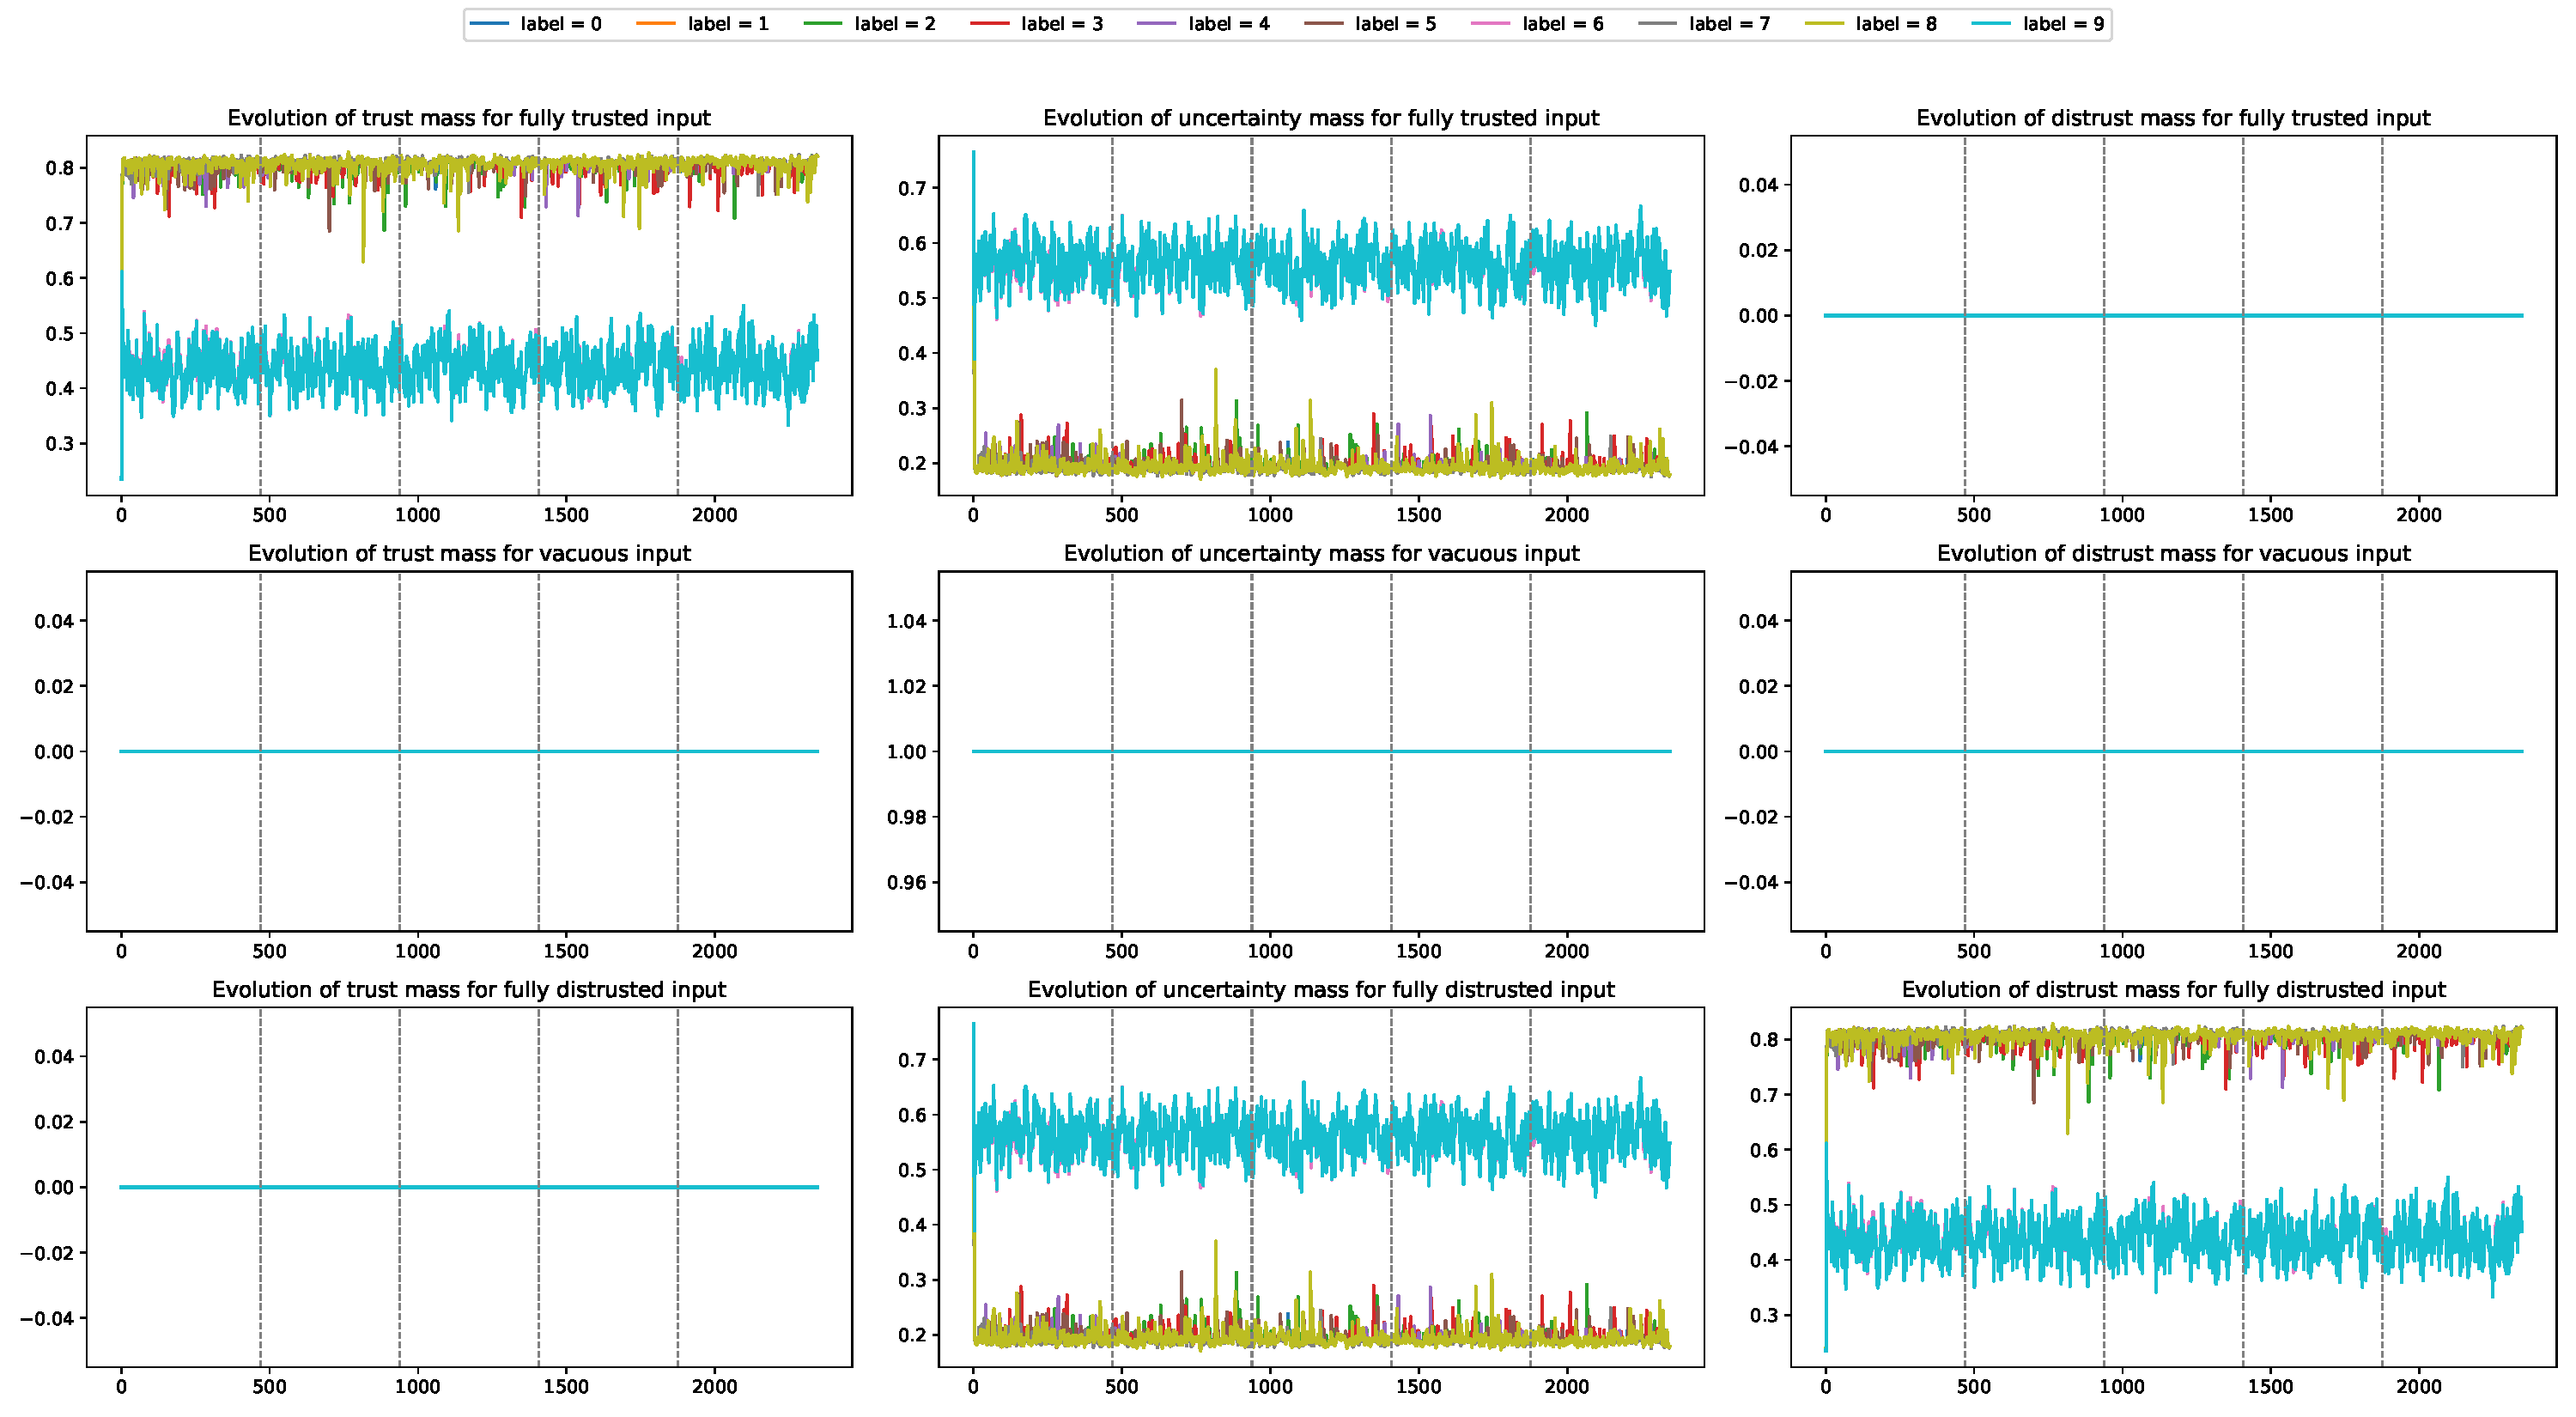
\includegraphics[width=0.8\textwidth]{latex/PTAS_Eval_mnist_128_trust_trust_eps_0.05_PathSize_10__plot_ptas.pdf}
\caption{mnist\_128\_trust\_trust, $\varepsilon$=0.05, ps=10}
\end{figure}

\begin{figure}[htbp]
\centering
  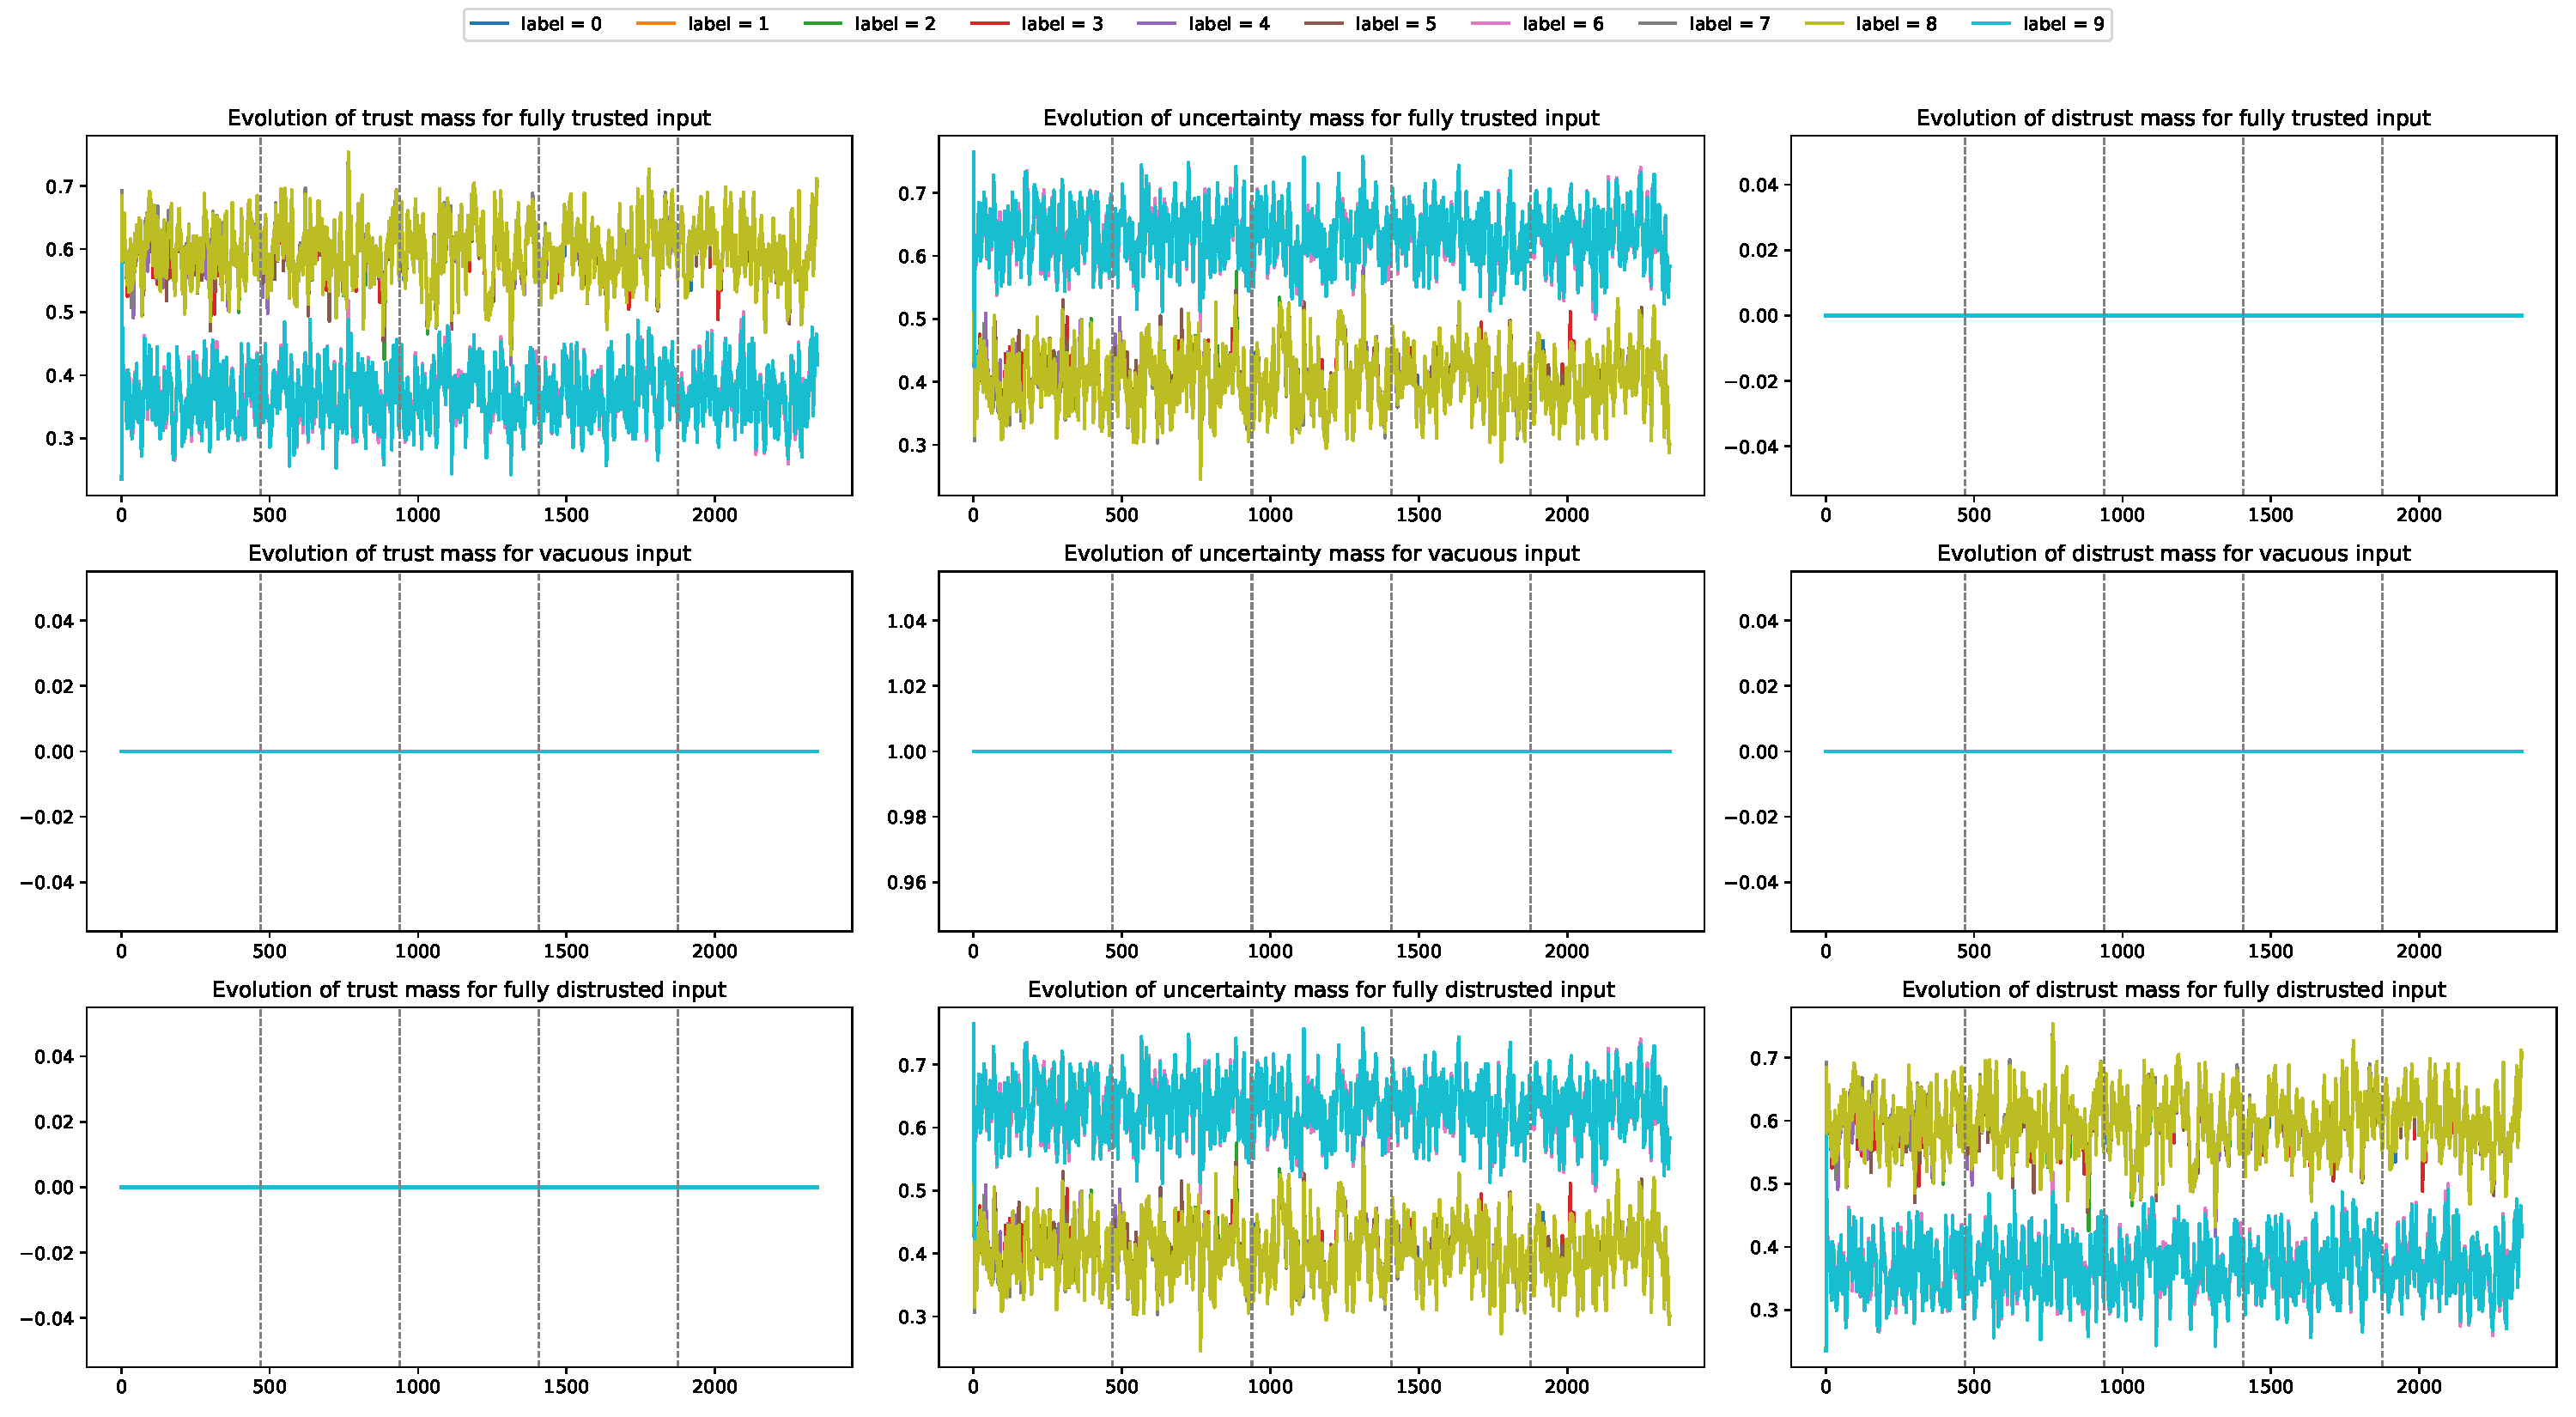
\includegraphics[width=0.8\textwidth]{latex/PTAS_Eval_mnist_128_trust_trust_eps_0.05_PathSize_27__plot_ptas.pdf}
\caption{mnist\_128\_trust\_trust, $\varepsilon$=0.05, ps=27}
\end{figure}

\begin{figure}[htbp]
\centering
  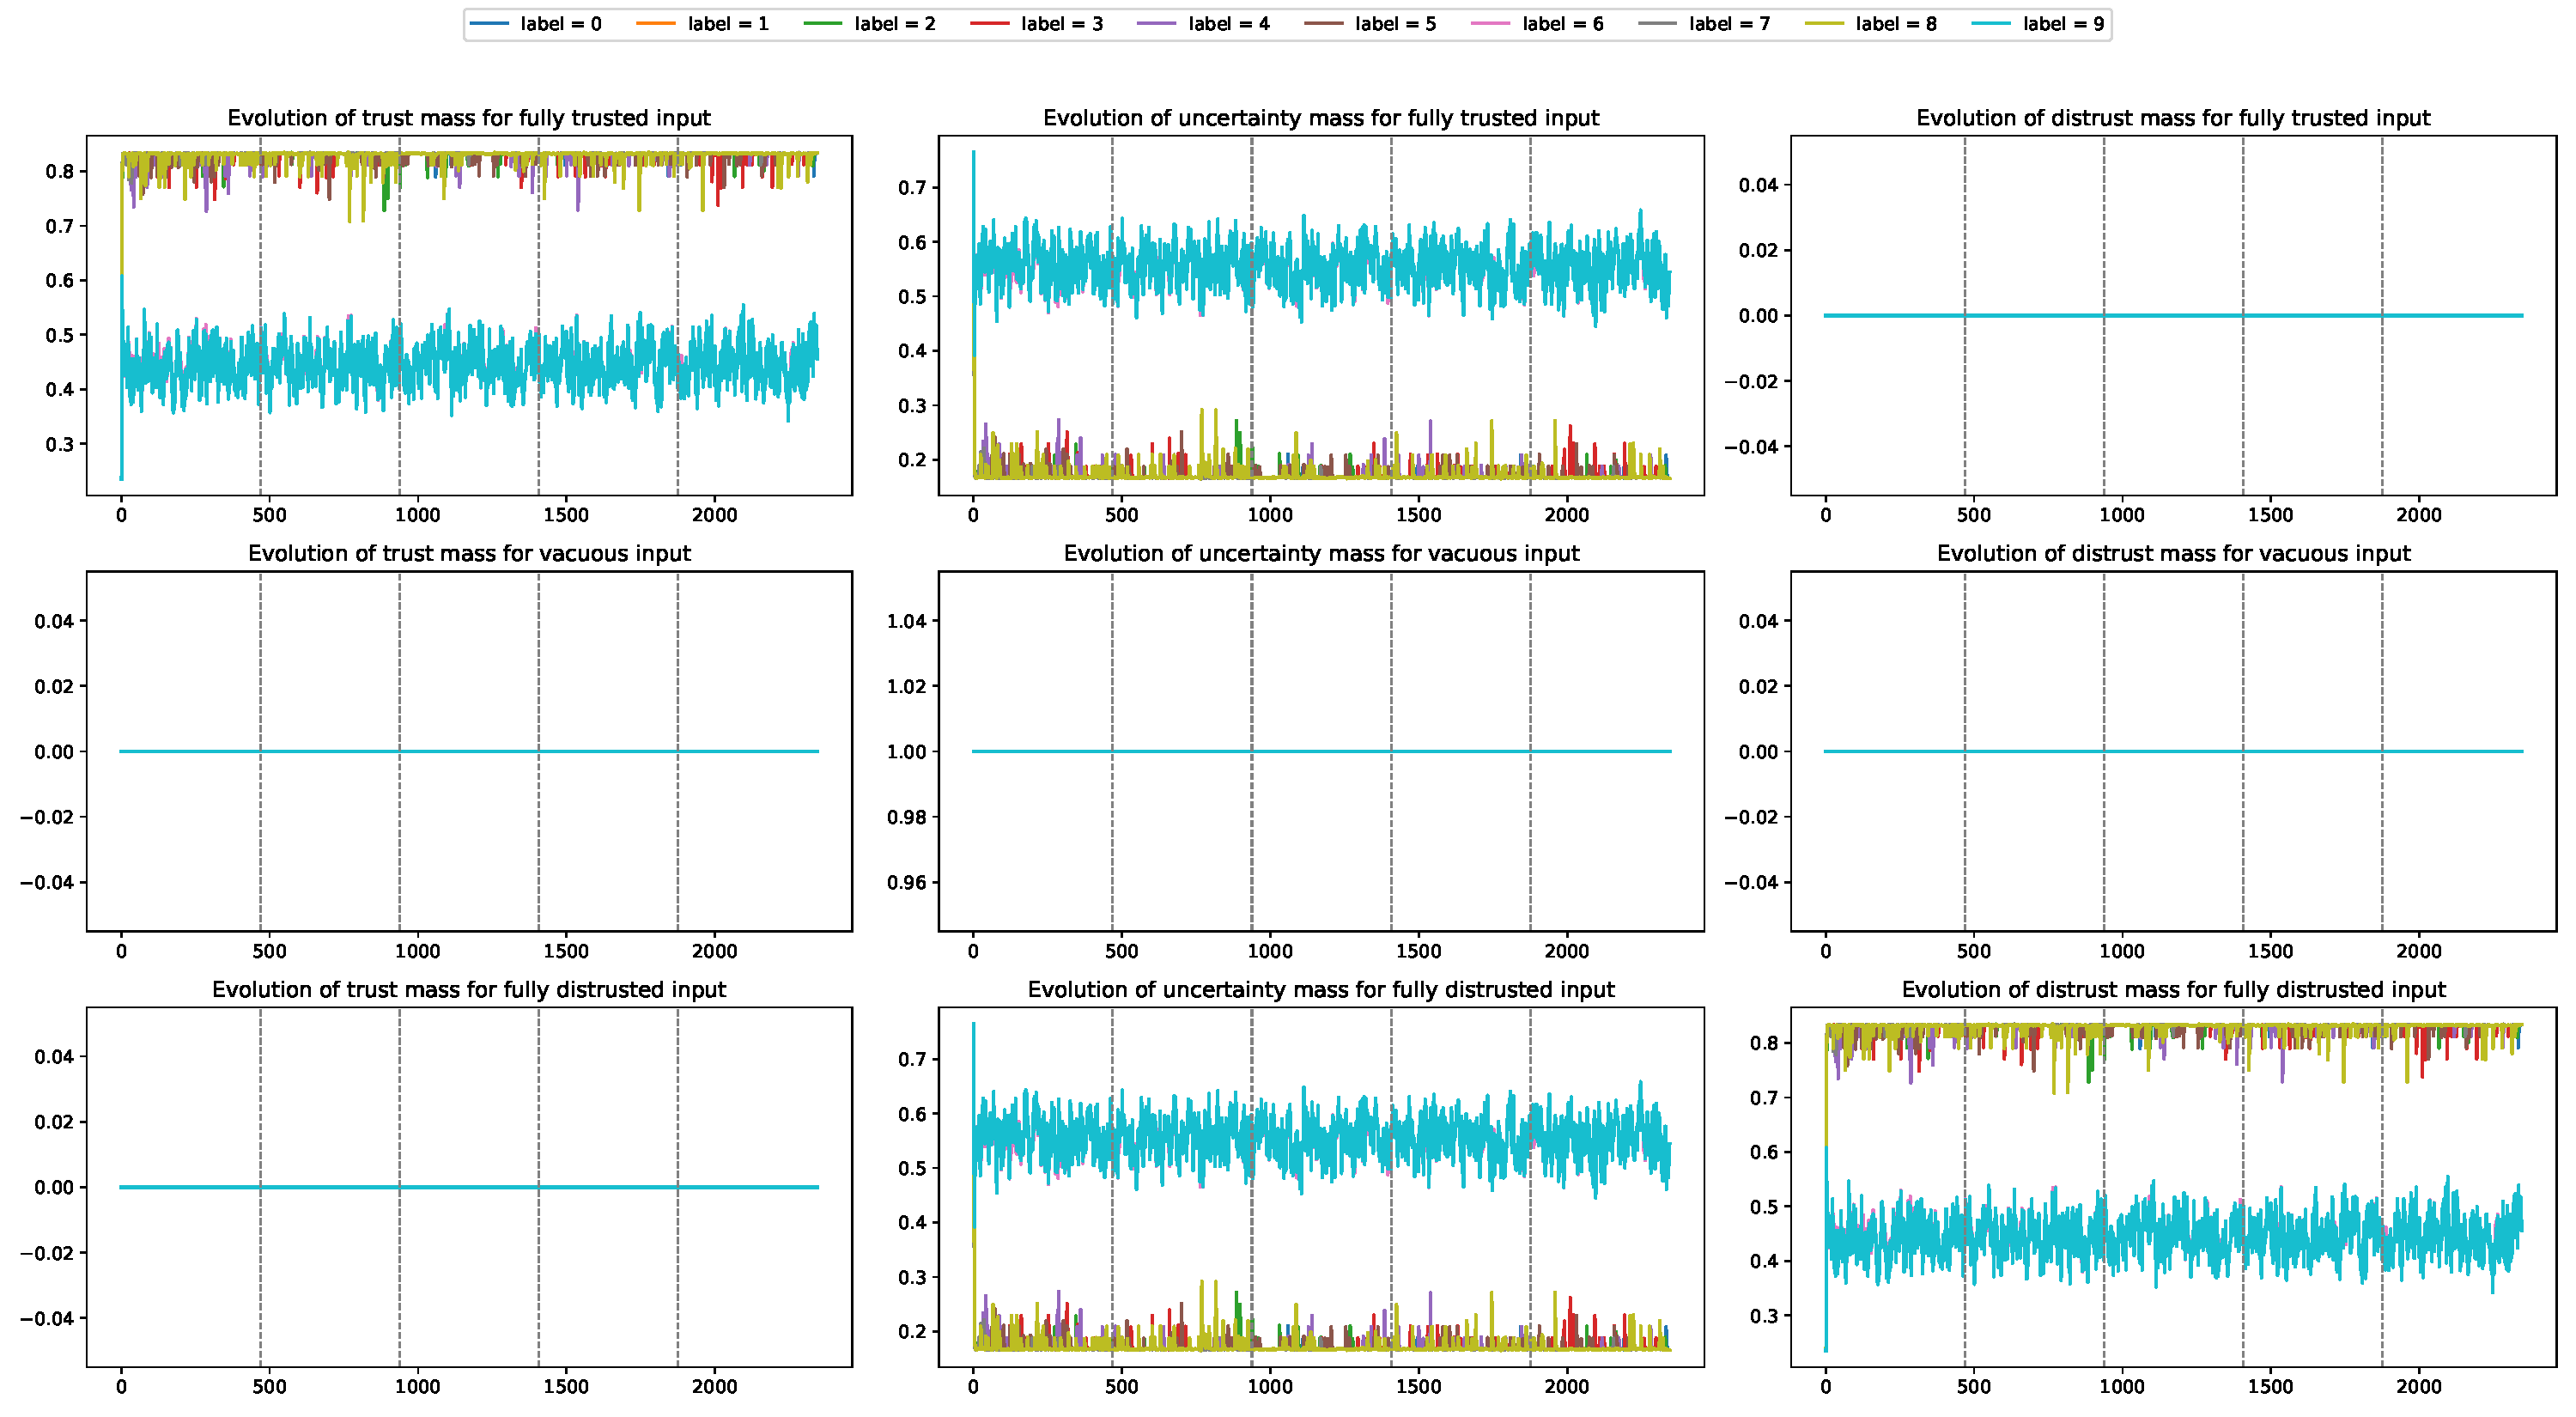
\includegraphics[width=0.8\textwidth]{latex/PTAS_Eval_mnist_128_trust_trust_eps_0.05_PathSize_4__plot_ptas.pdf}
\caption{mnist\_128\_trust\_trust, $\varepsilon$=0.05, ps=4}
\end{figure}

\begin{figure}[htbp]
\centering
  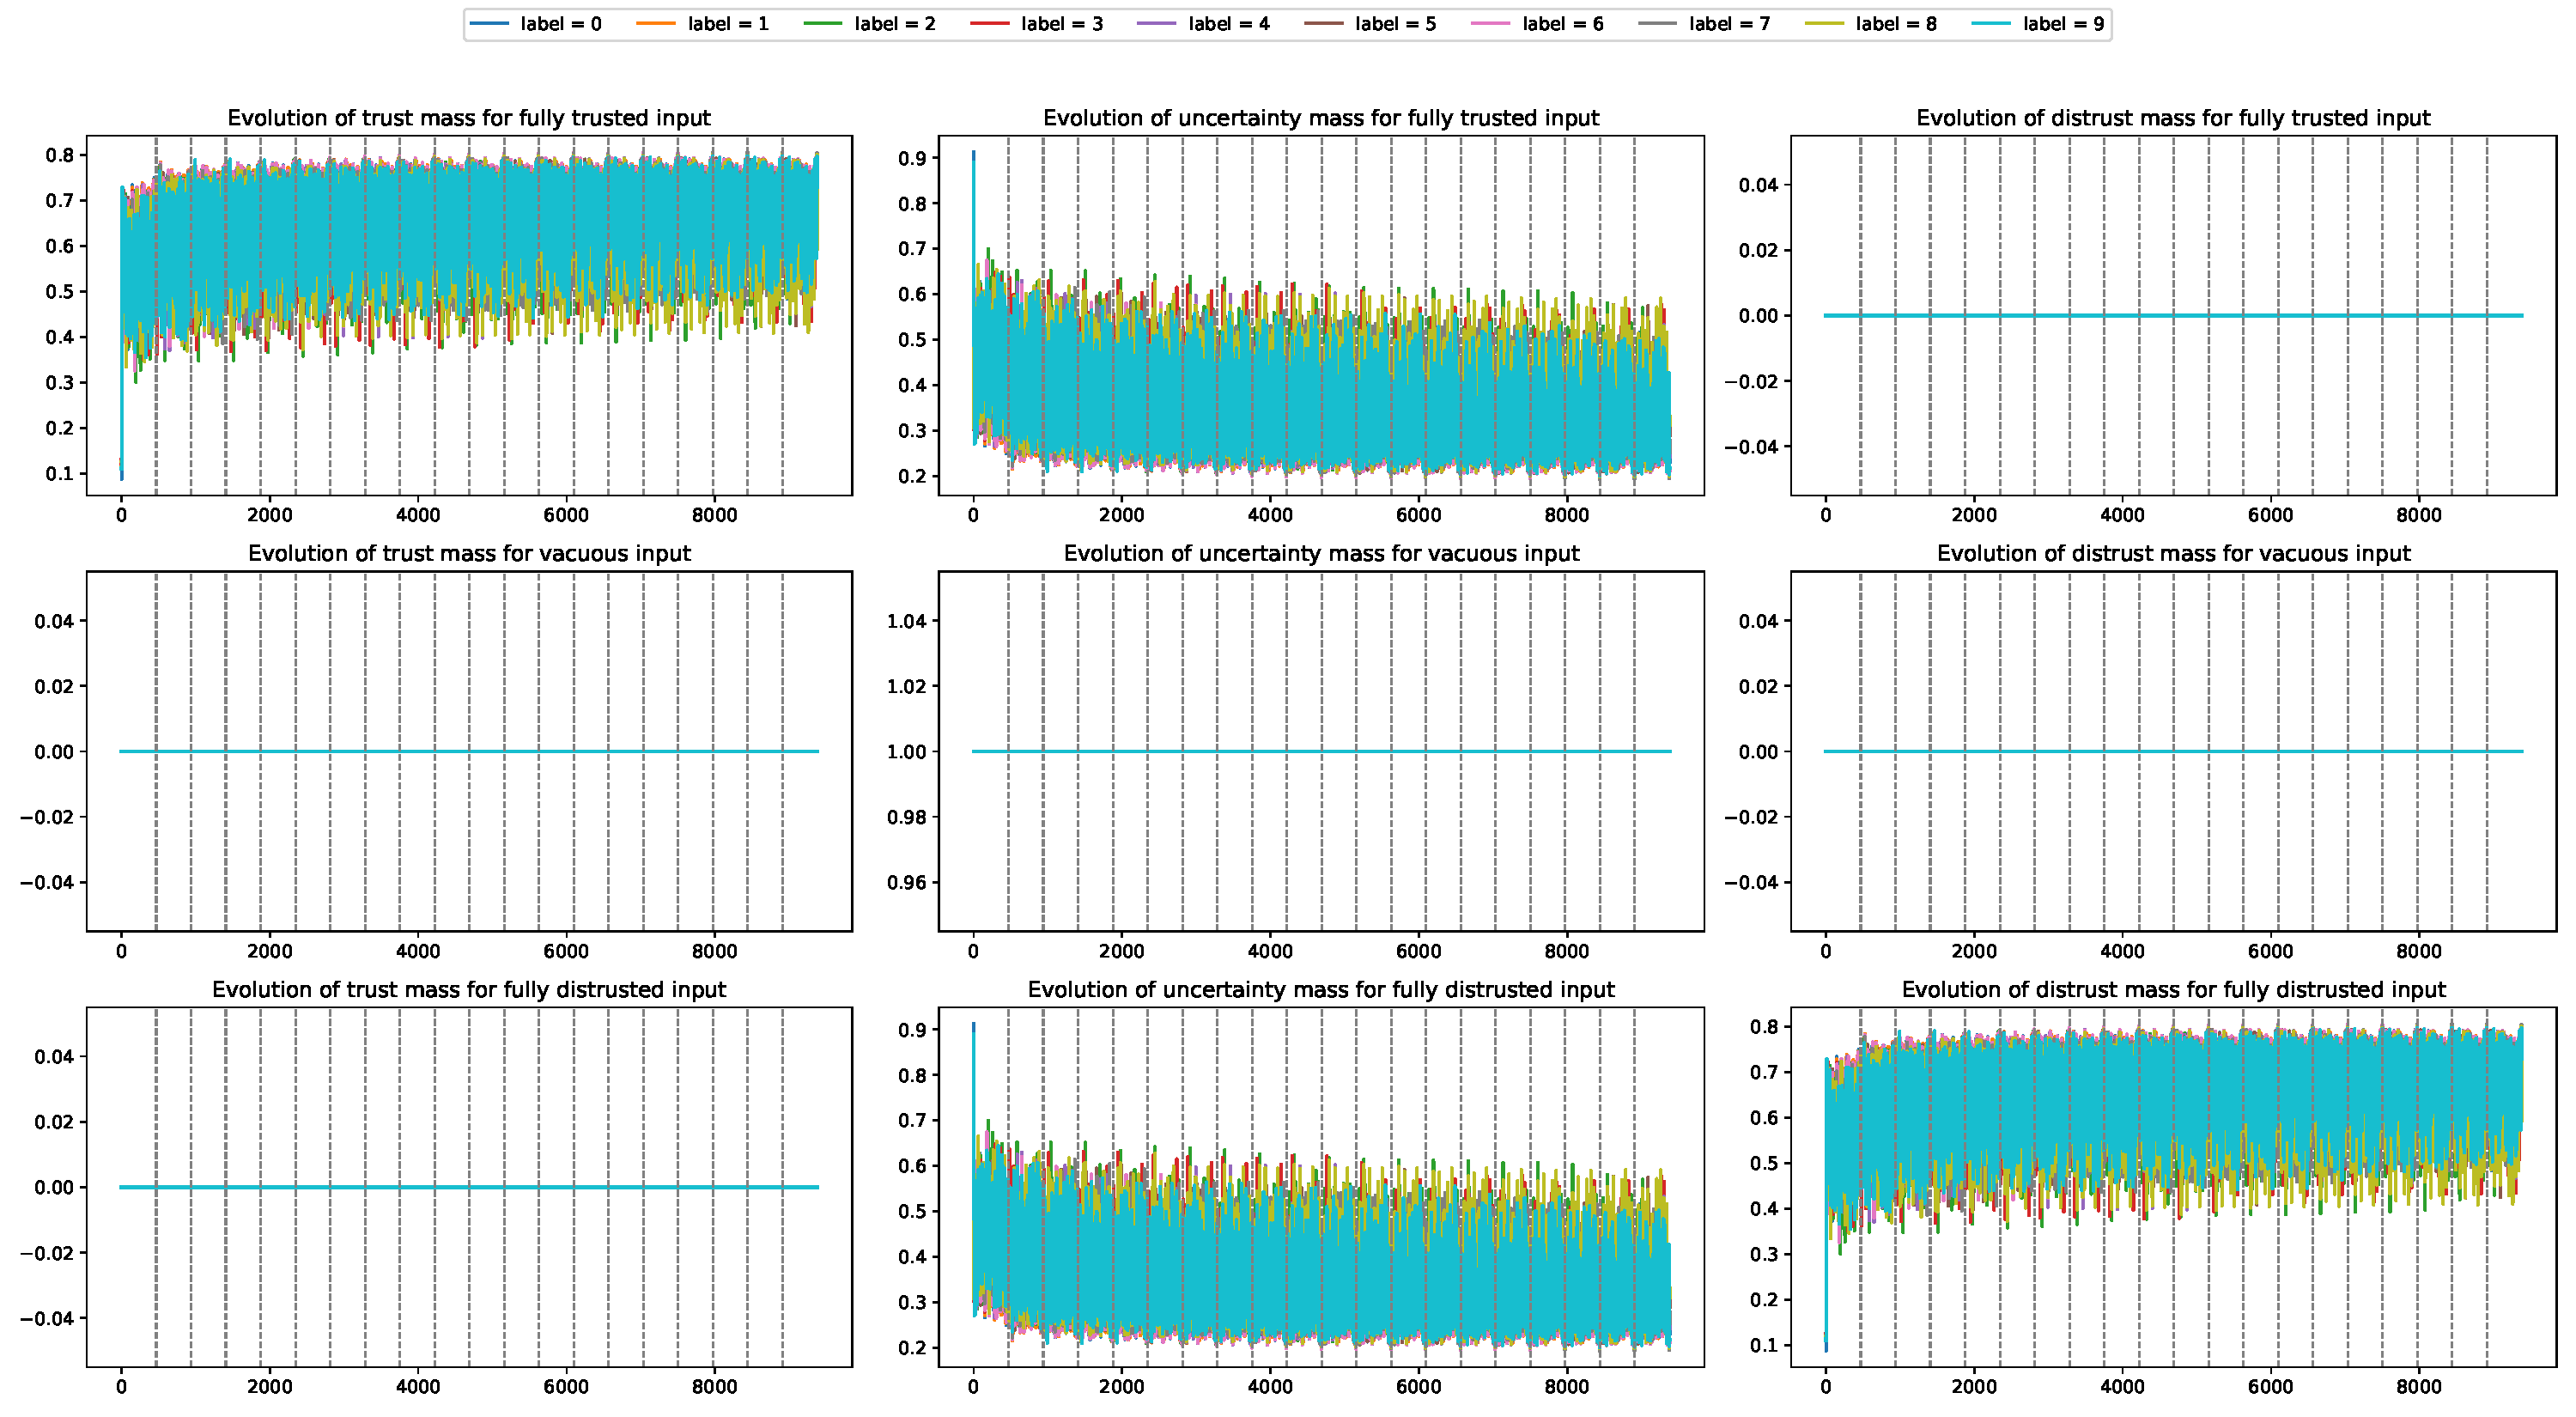
\includegraphics[width=0.8\textwidth]{latex/PTAS_Eval_mnist_16_16_trust_trust_eps_0.05_PathSize_None__plot_ptas.pdf}
\caption{mnist\_16\_16\_trust\_trust, $\varepsilon$=0.05}
\end{figure}

\begin{figure}[htbp]
\centering
  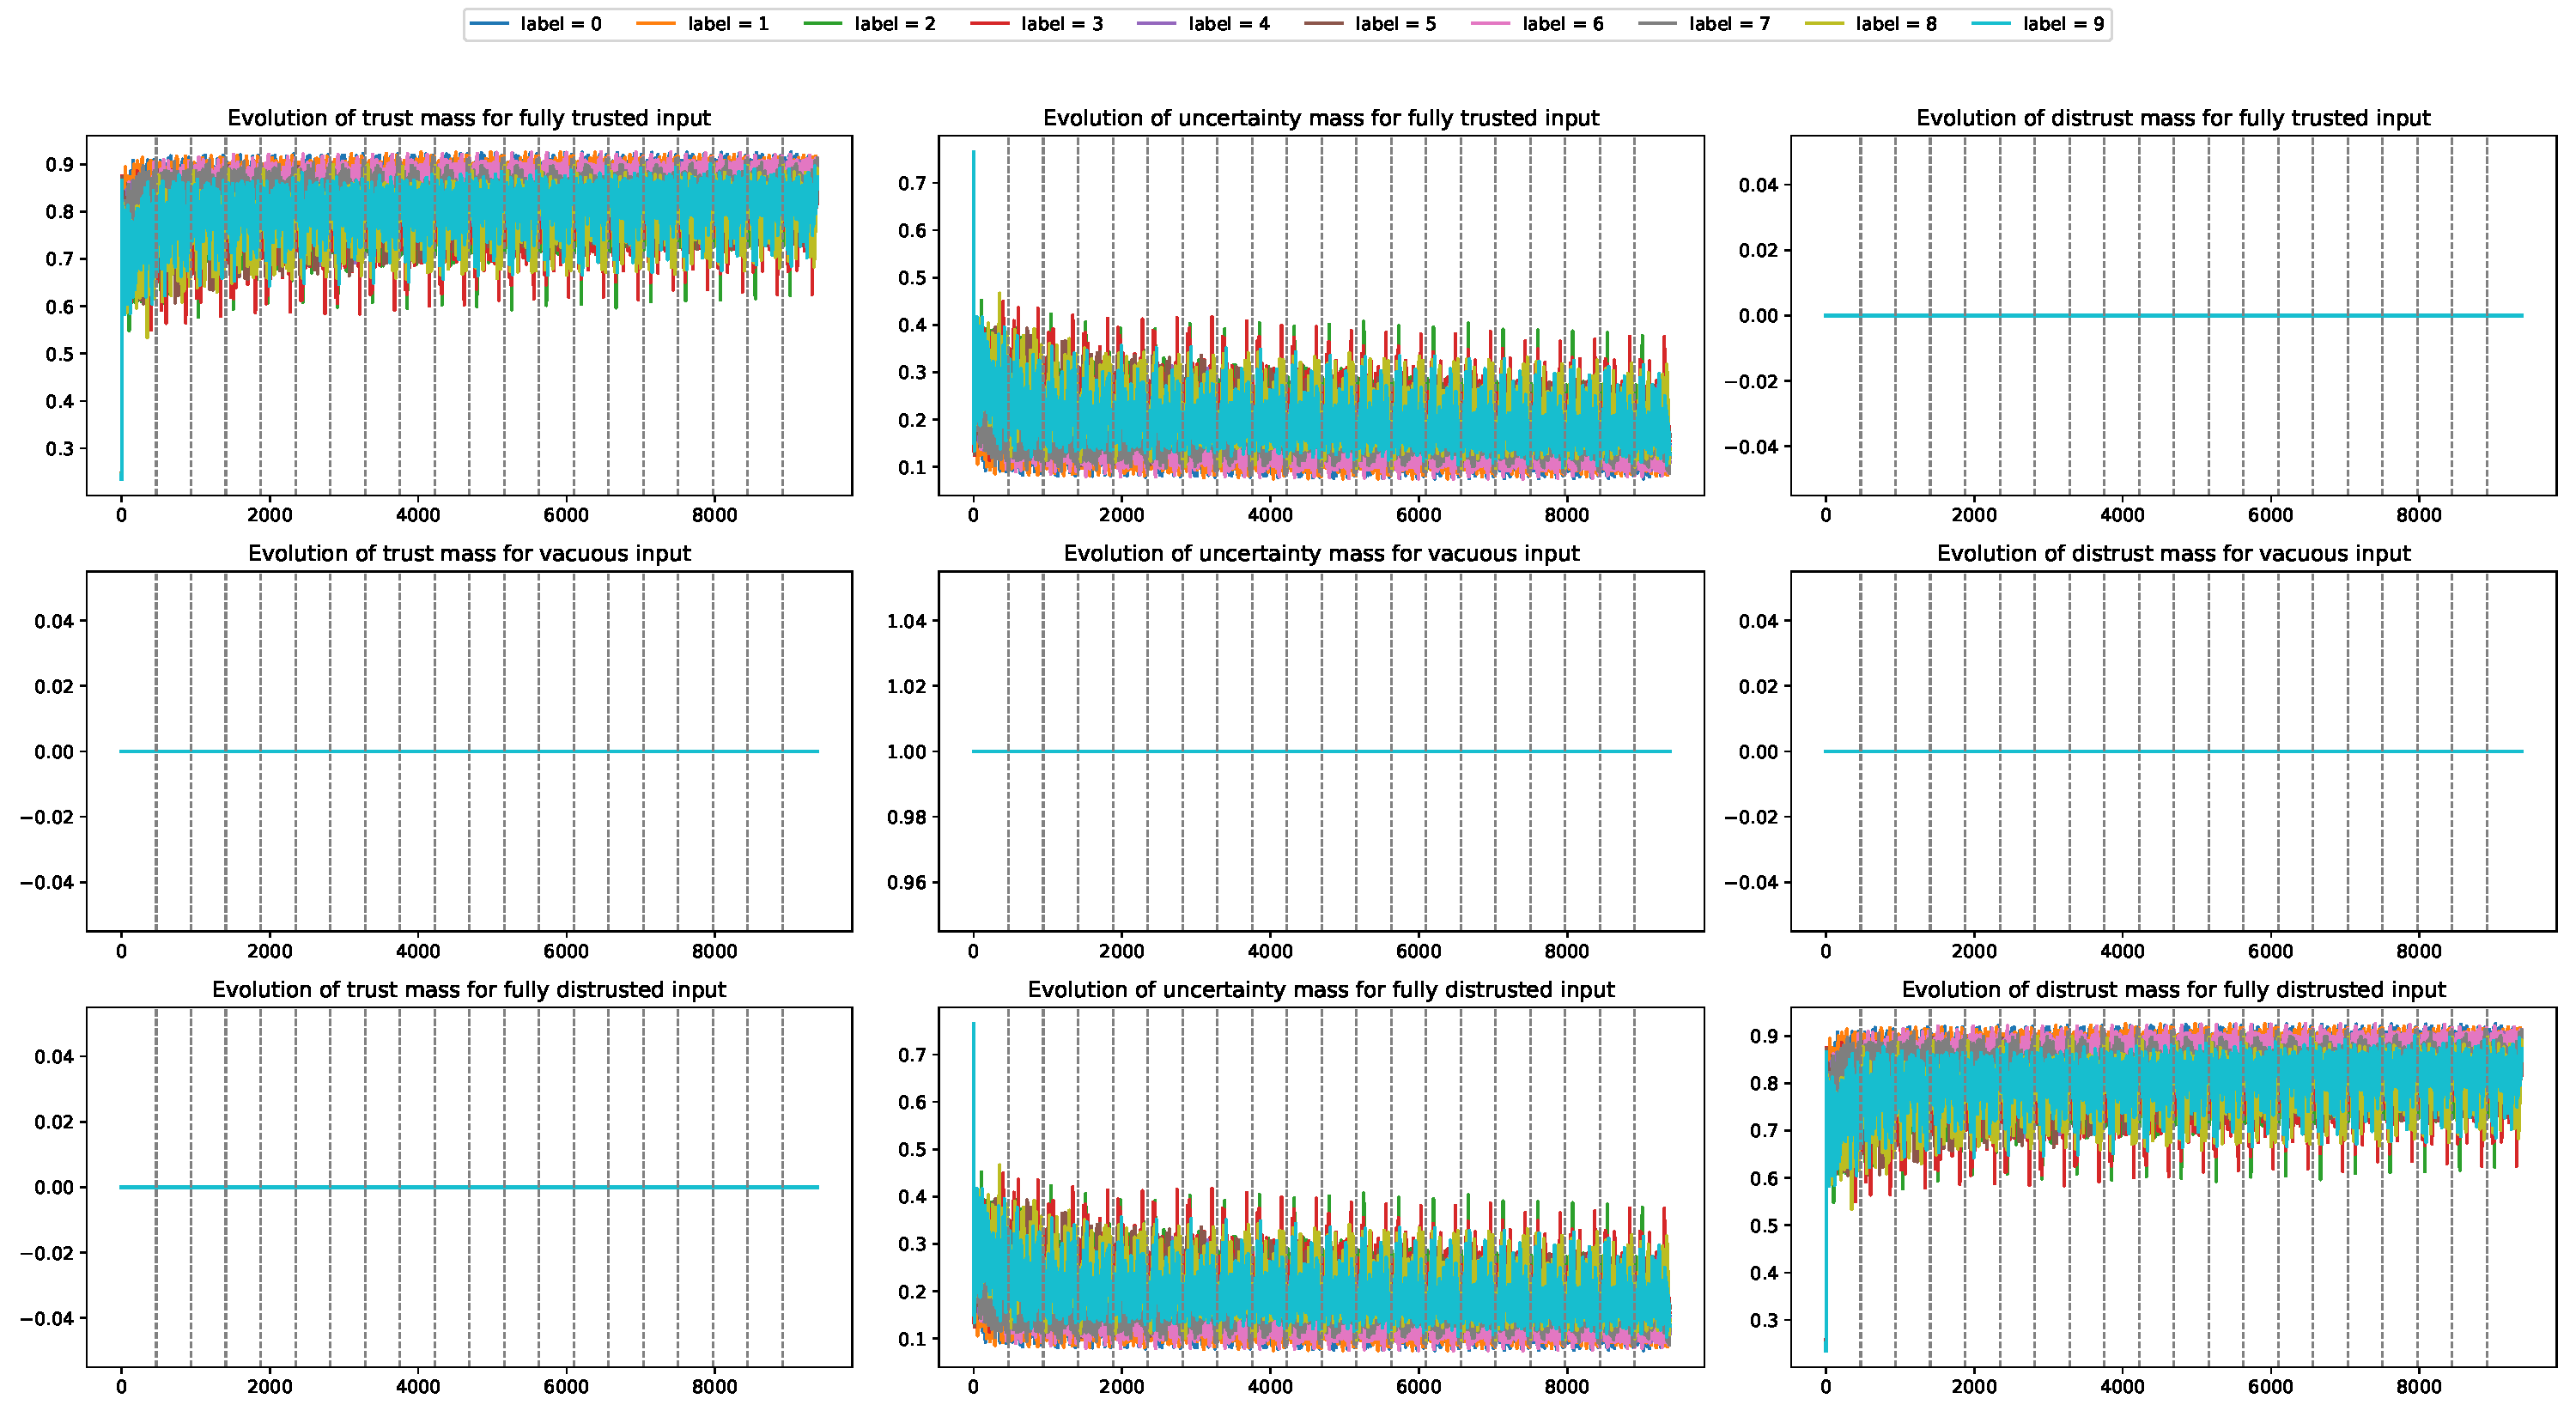
\includegraphics[width=0.8\textwidth]{latex/PTAS_Eval_mnist_16_trust_trust_eps_0.05_PathSize_None__plot_ptas.pdf}
\caption{mnist\_16\_trust\_trust, $\varepsilon$=0.05}
\end{figure}

\subsubsection{vacuous -- vacuous}

\begin{figure}[htbp]
\centering
  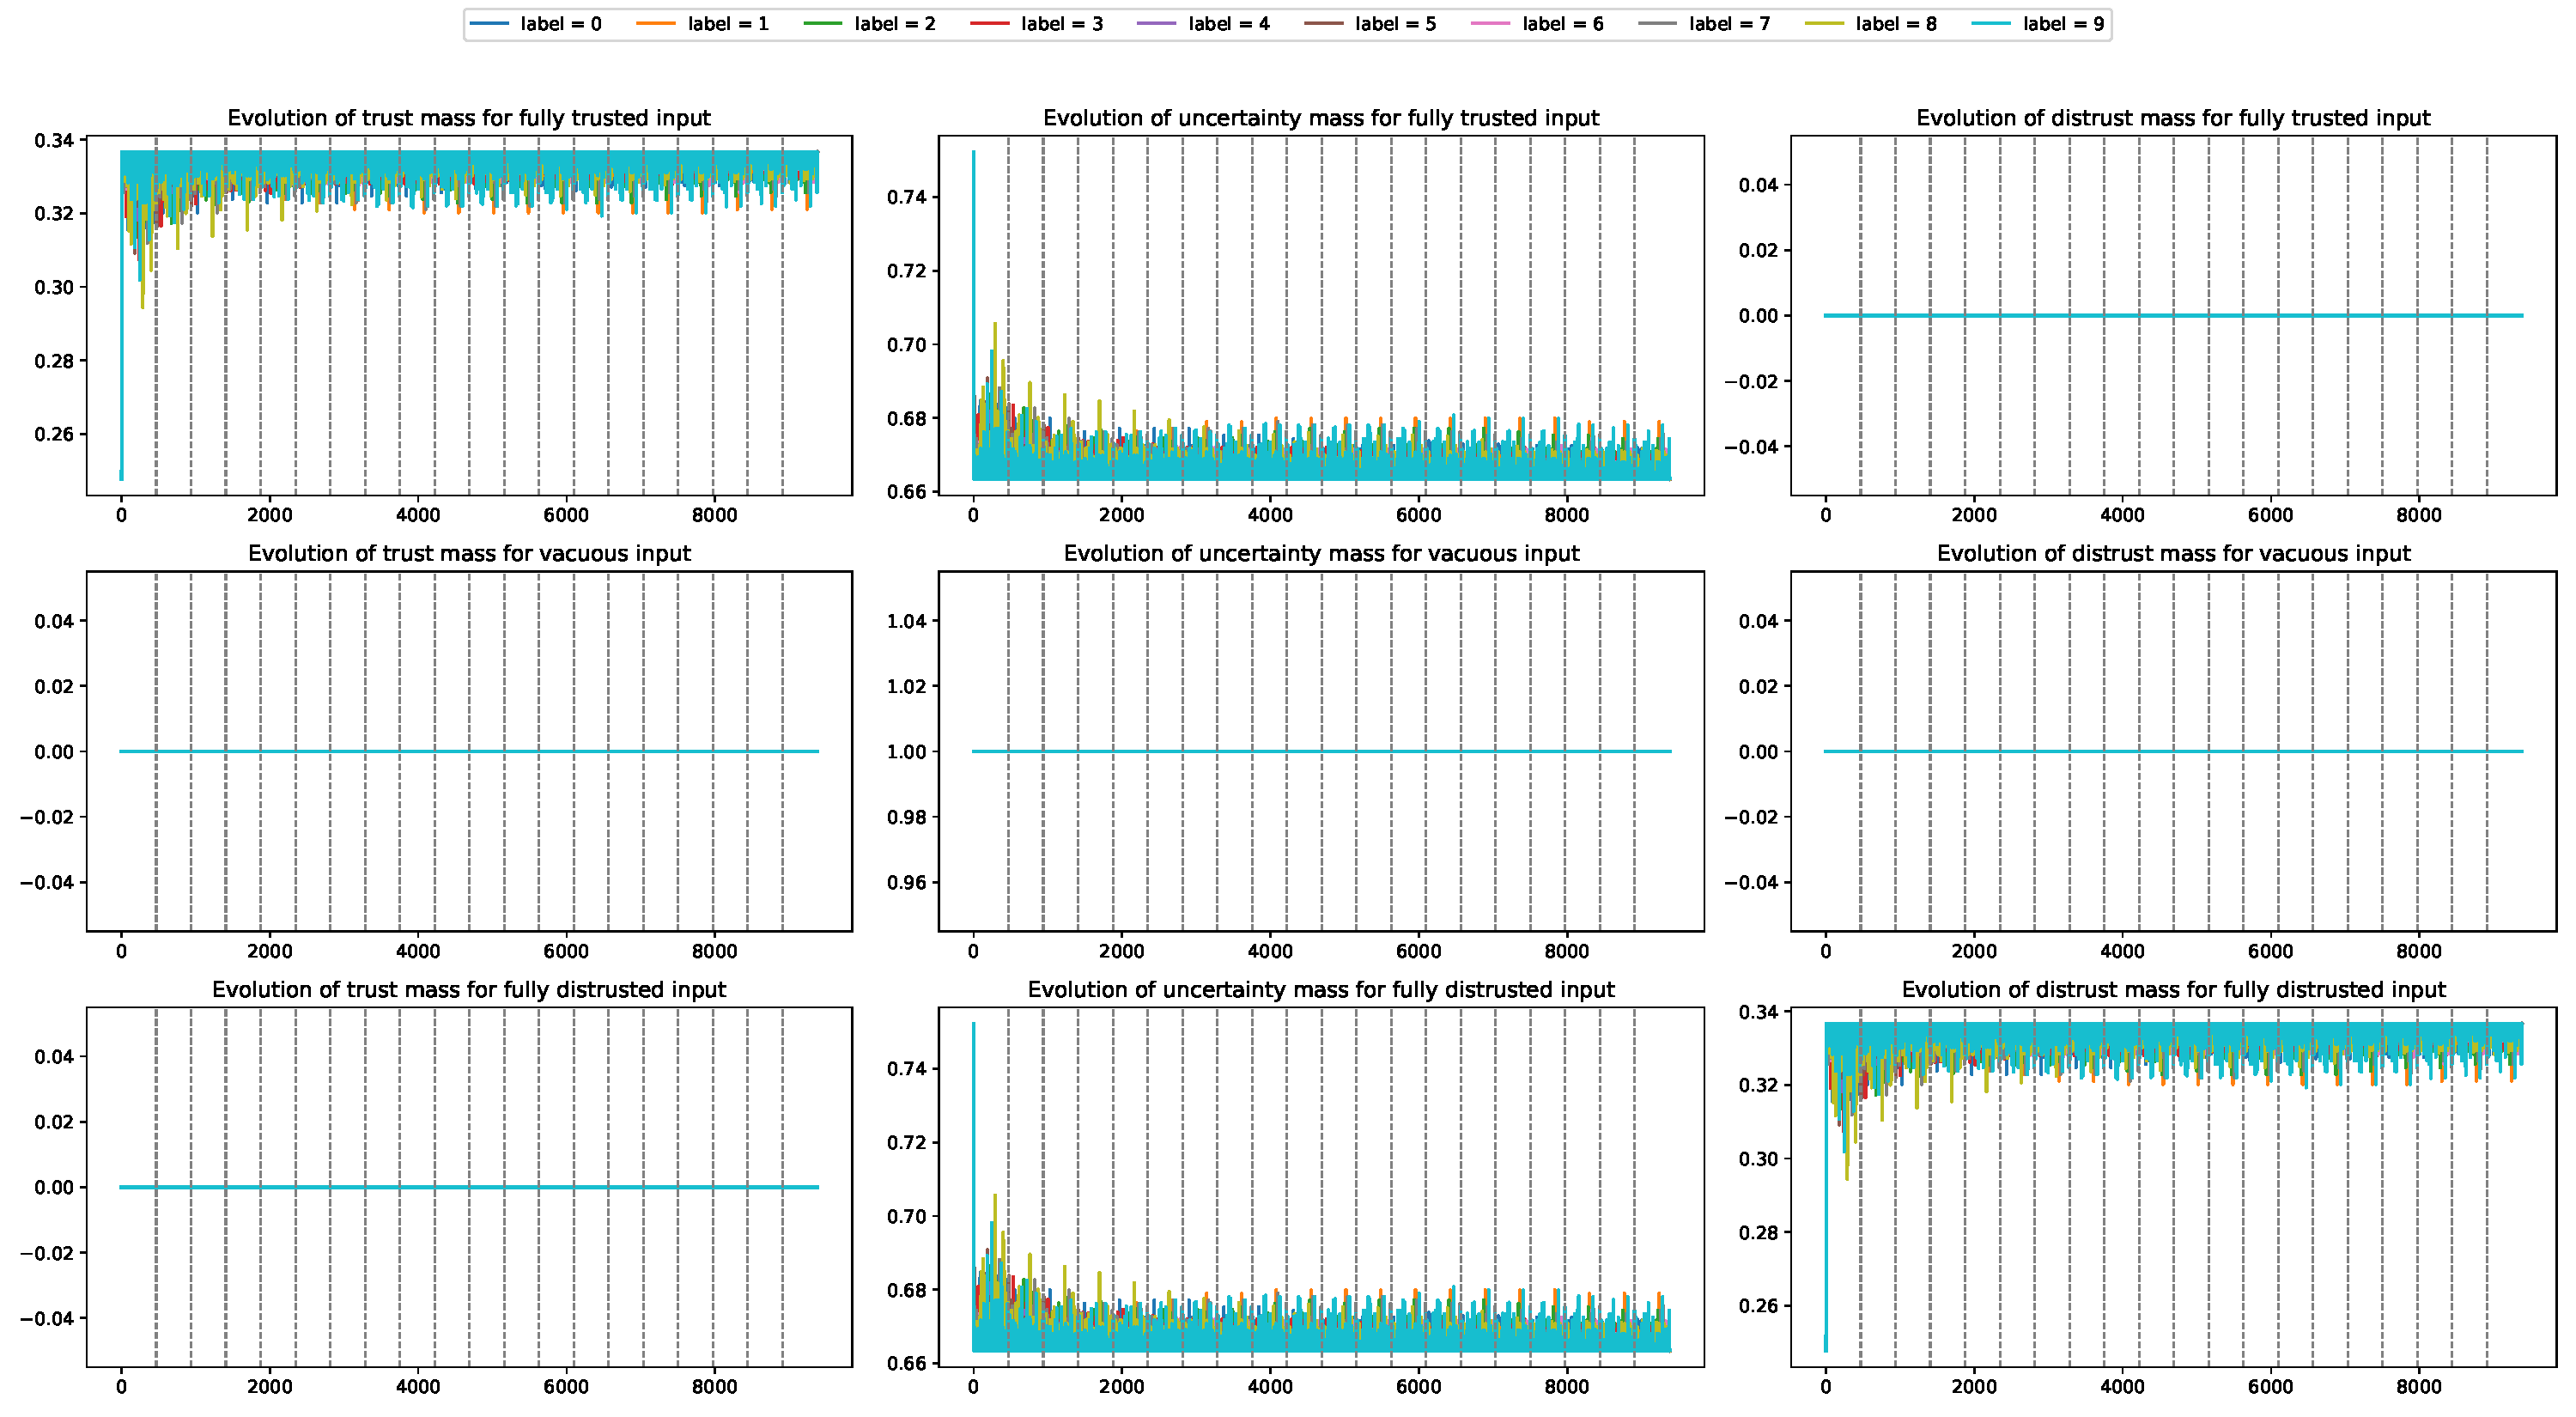
\includegraphics[width=0.8\textwidth]{latex/PTAS_Eval_mnist_128_vacuous_vacuous_eps_0.05_PathSize_None__plot_ptas.pdf}
\caption{mnist\_128\_vacuous\_vacuous, $\varepsilon$=0.05}
\end{figure}

\begin{figure}[htbp]
\centering
  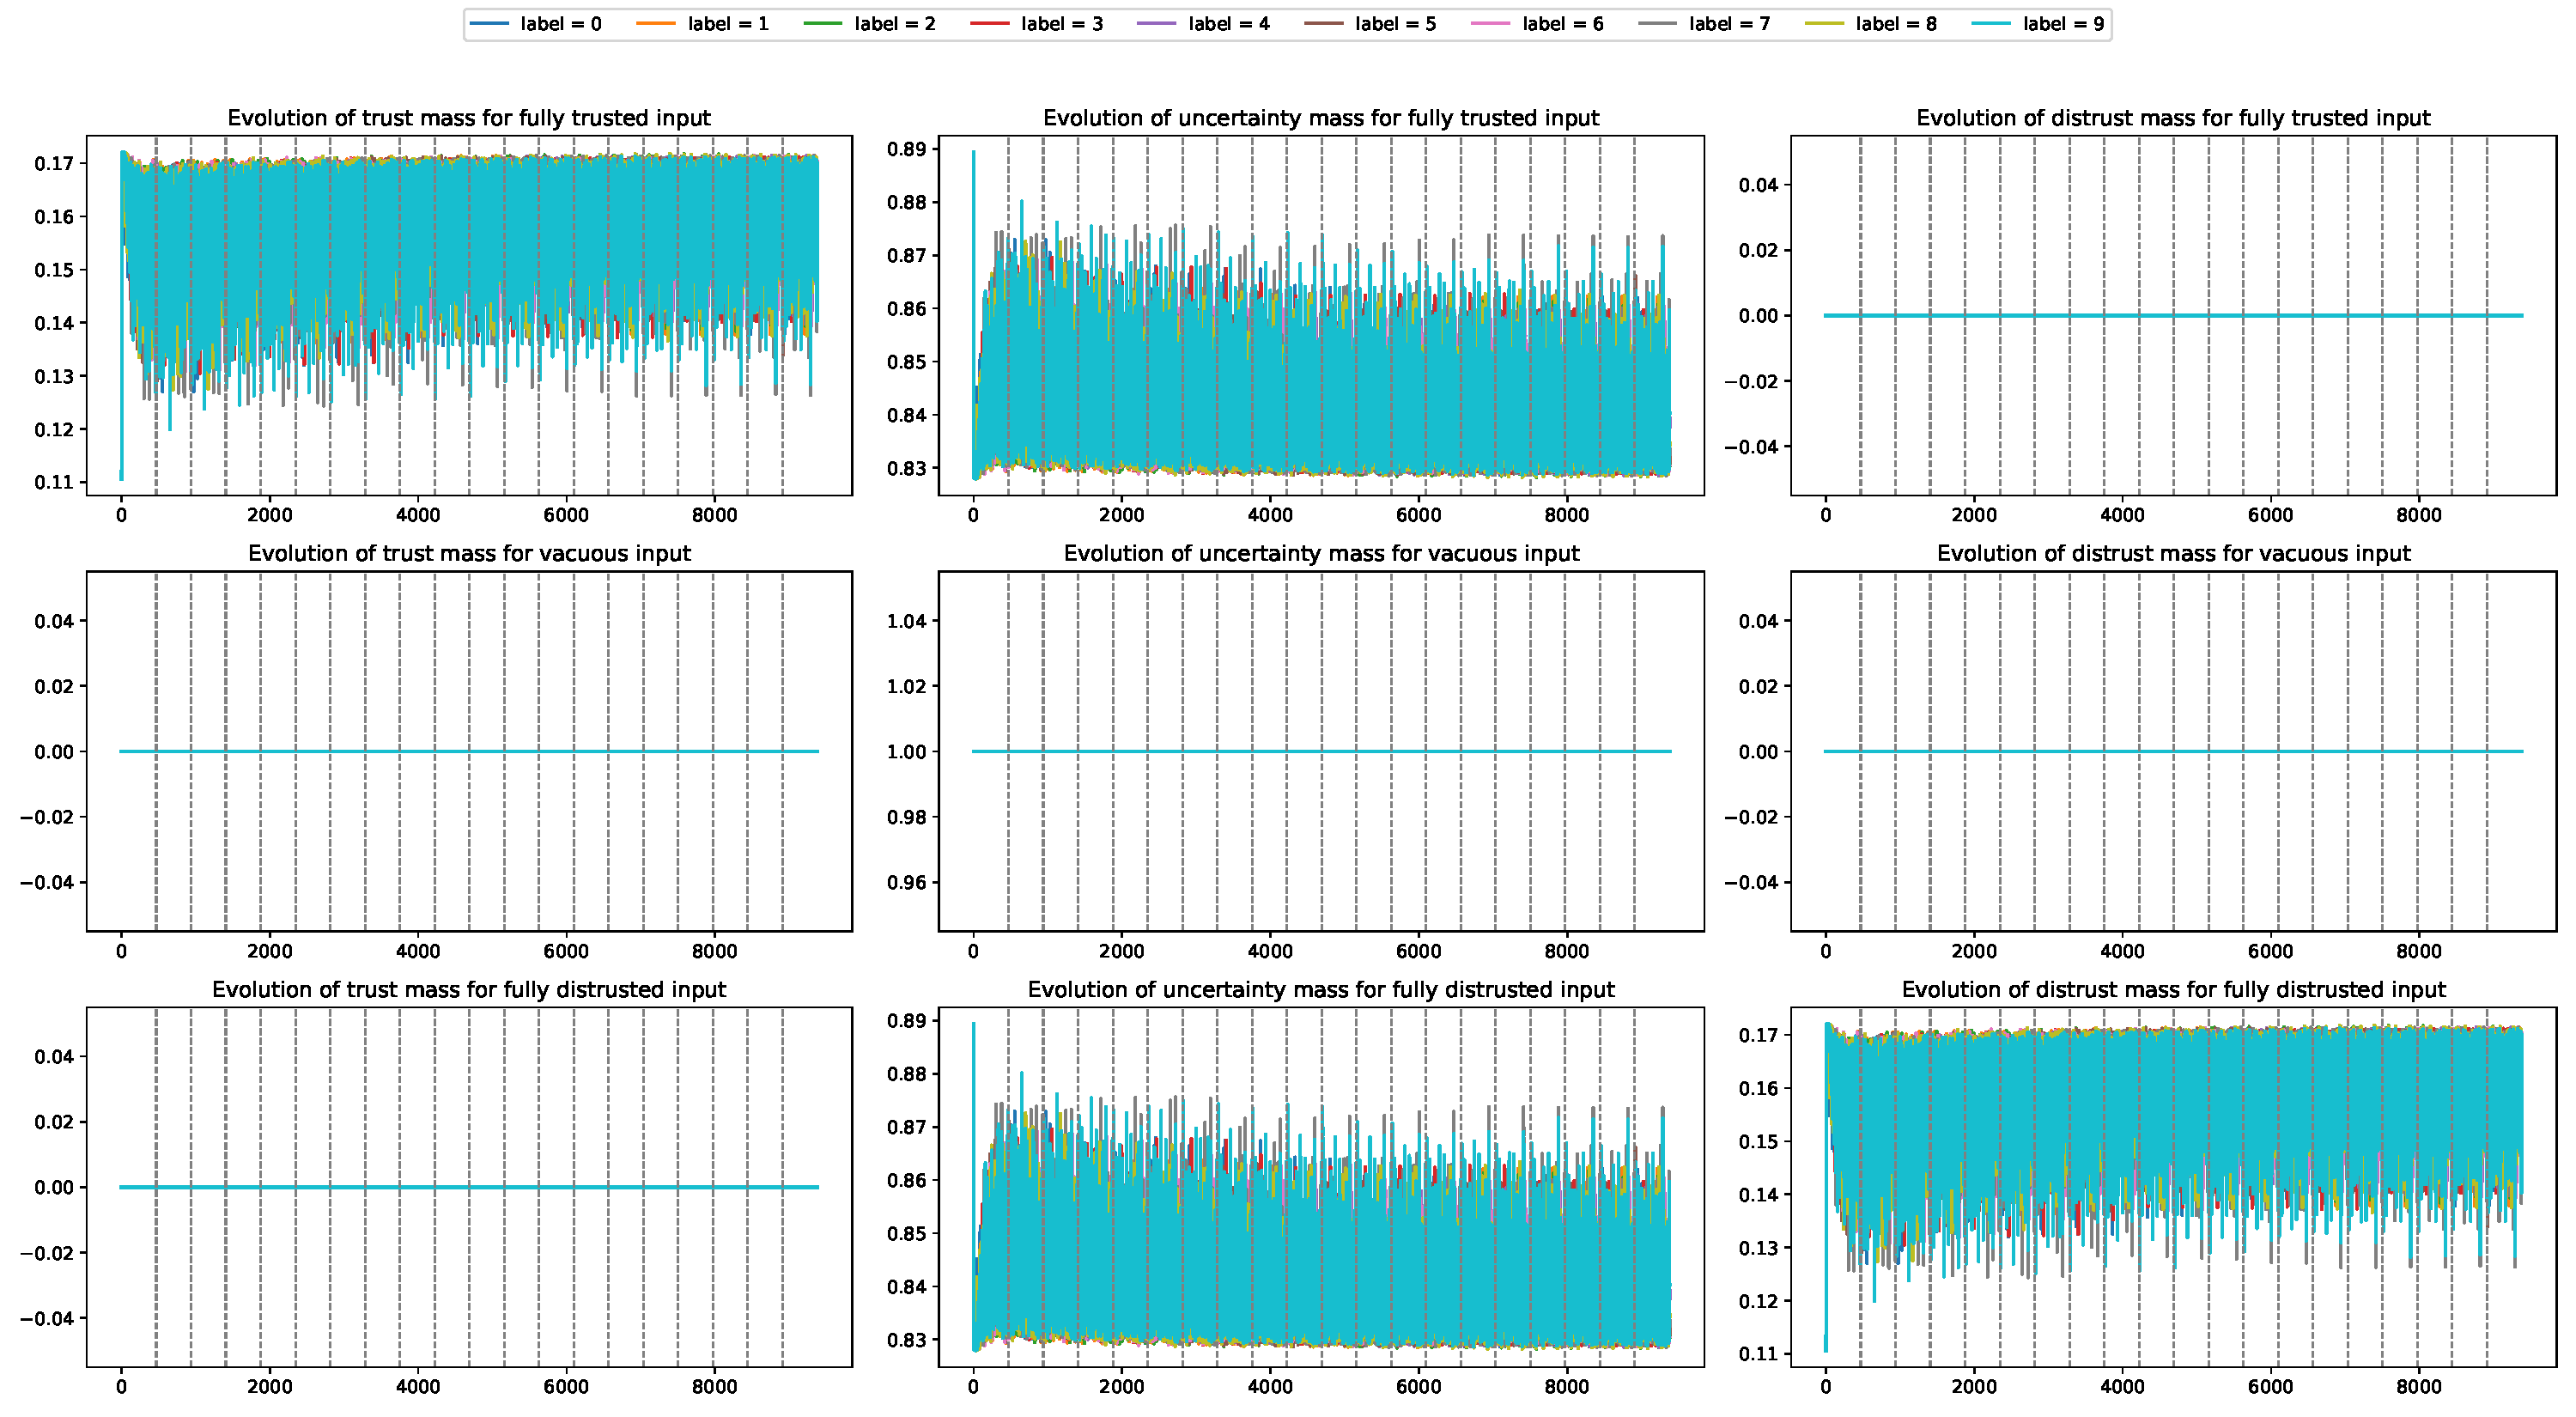
\includegraphics[width=0.8\textwidth]{latex/PTAS_Eval_mnist_16_16_vacuous_vacuous_eps_0.05_PathSize_None__plot_ptas.pdf}
\caption{mnist\_16\_16\_vacuous\_vacuous, $\varepsilon$=0.05}
\end{figure}

\begin{figure}[htbp]
\centering
  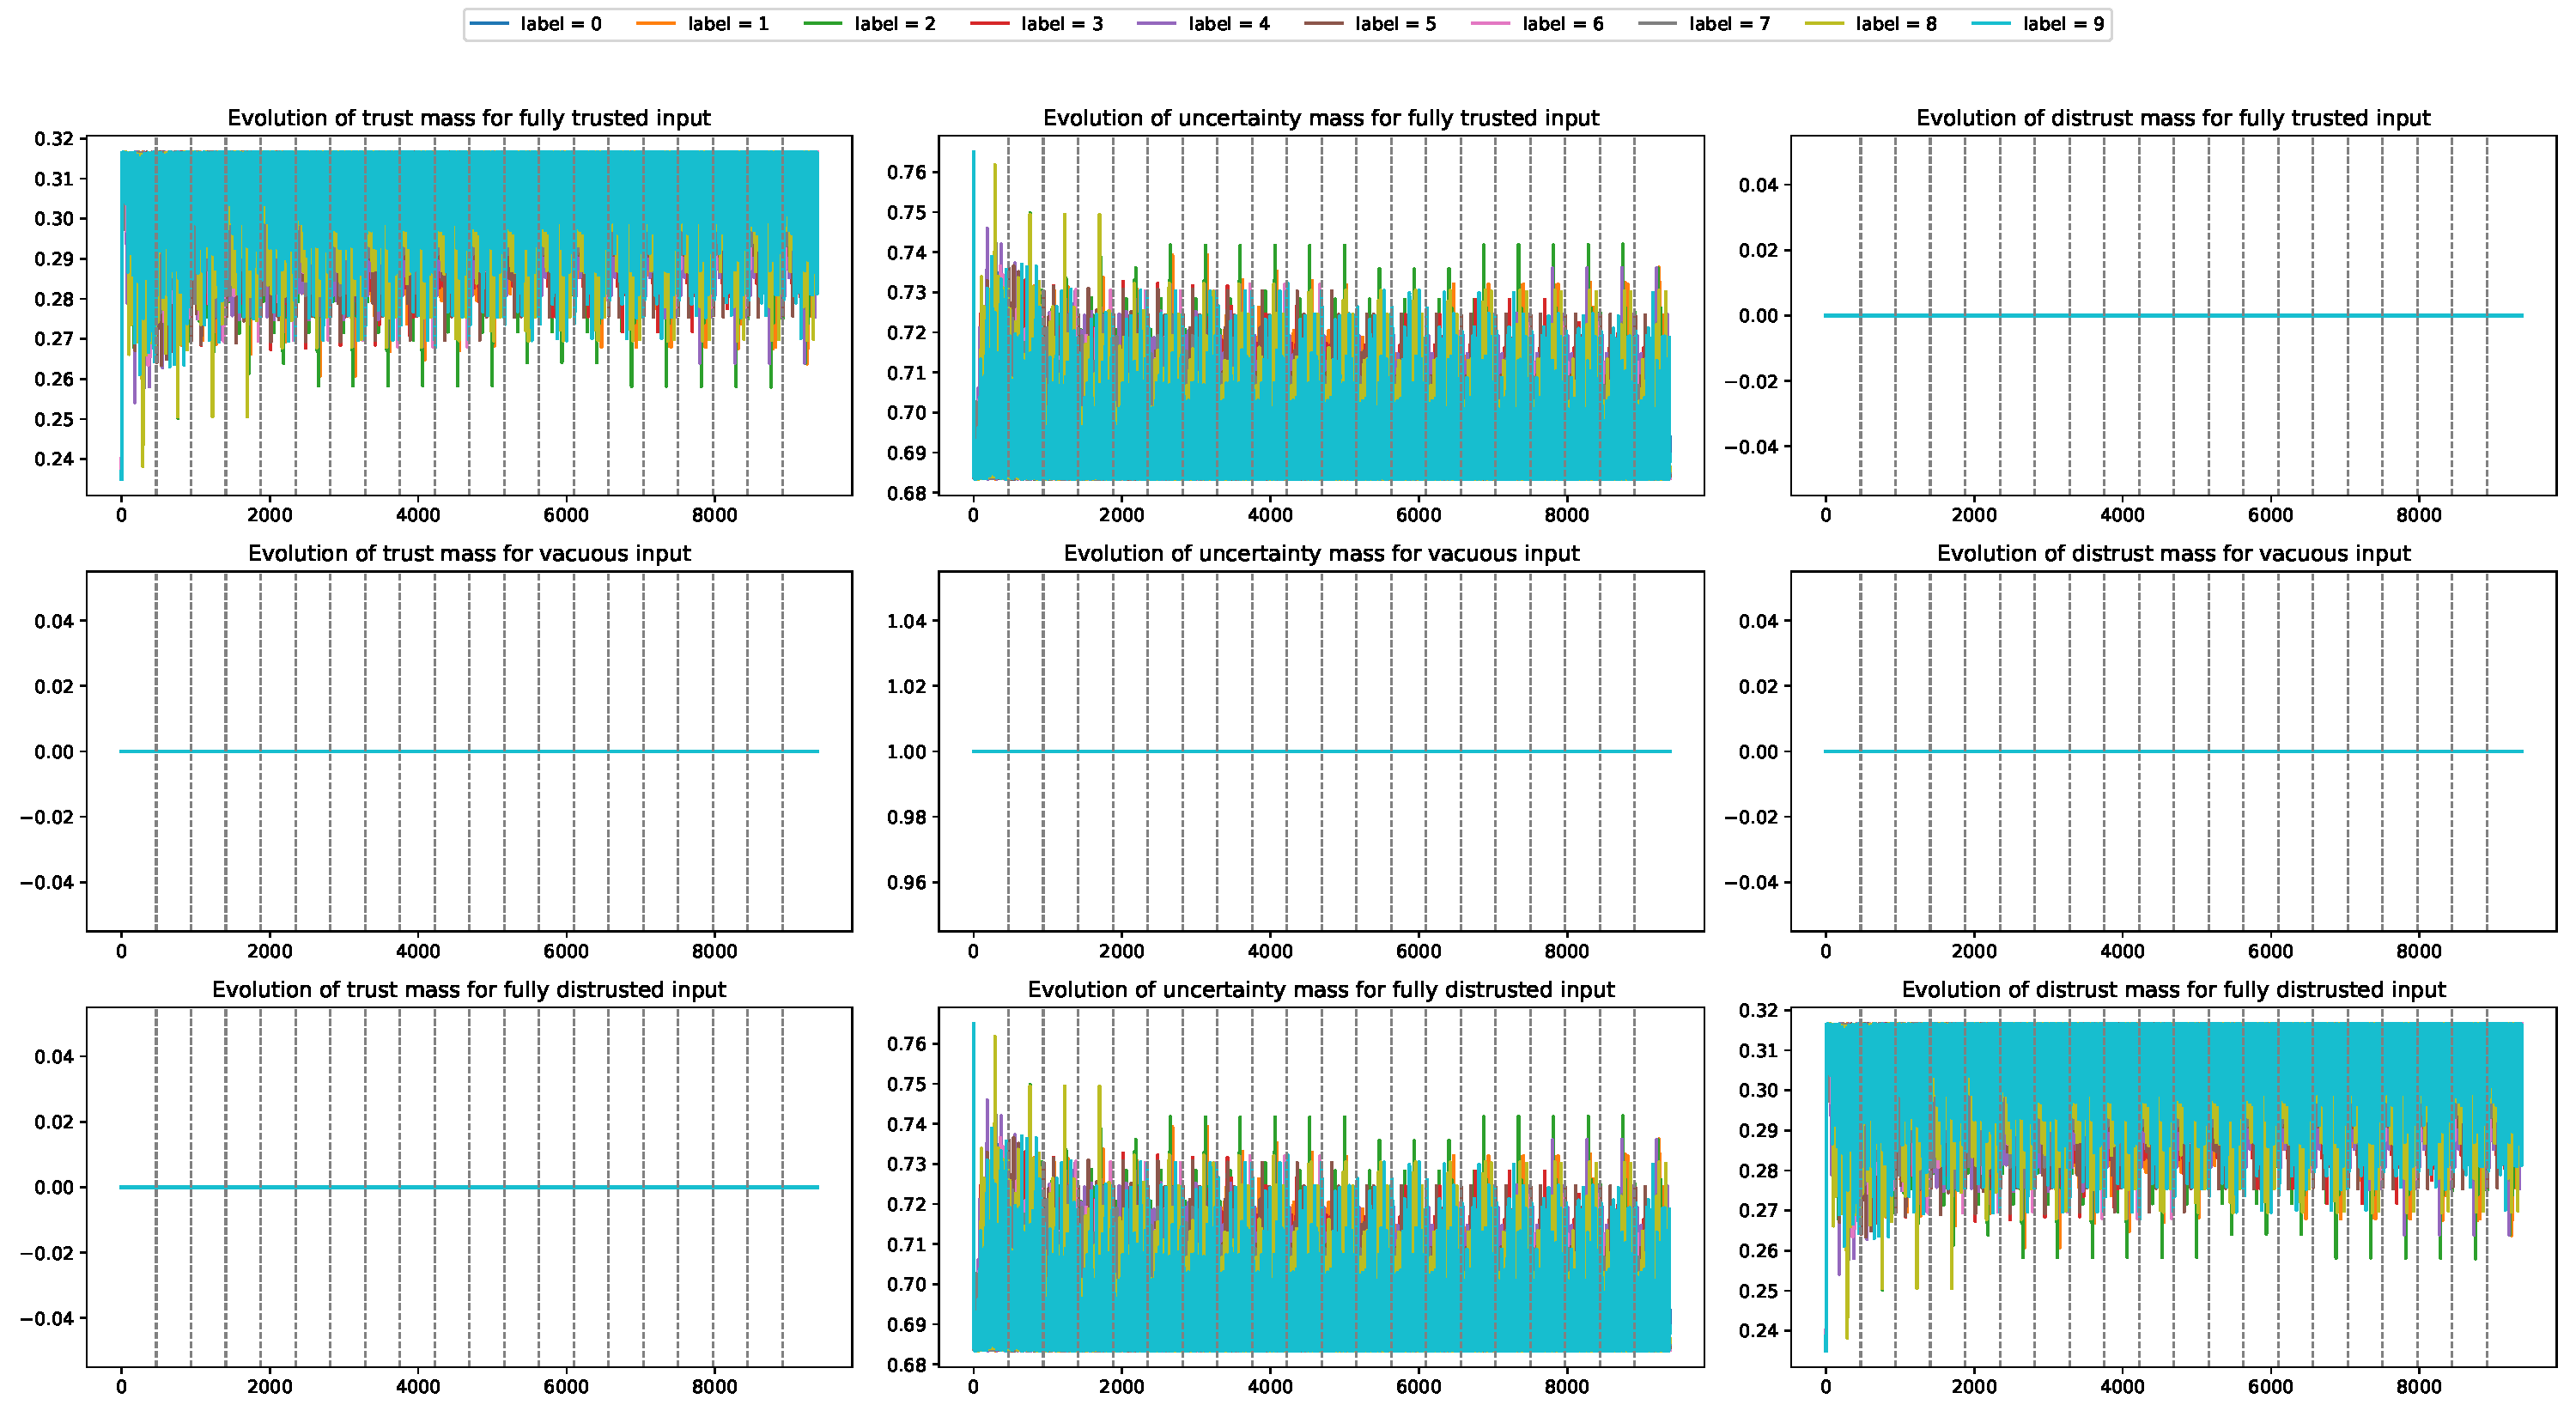
\includegraphics[width=0.8\textwidth]{latex/PTAS_Eval_mnist_16_vacuous_vacuous_eps_0.05_PathSize_None__plot_ptas.pdf}
\caption{mnist\_16\_vacuous\_vacuous, $\varepsilon$=0.05}
\end{figure}

\begin{figure}[htbp]
\centering
  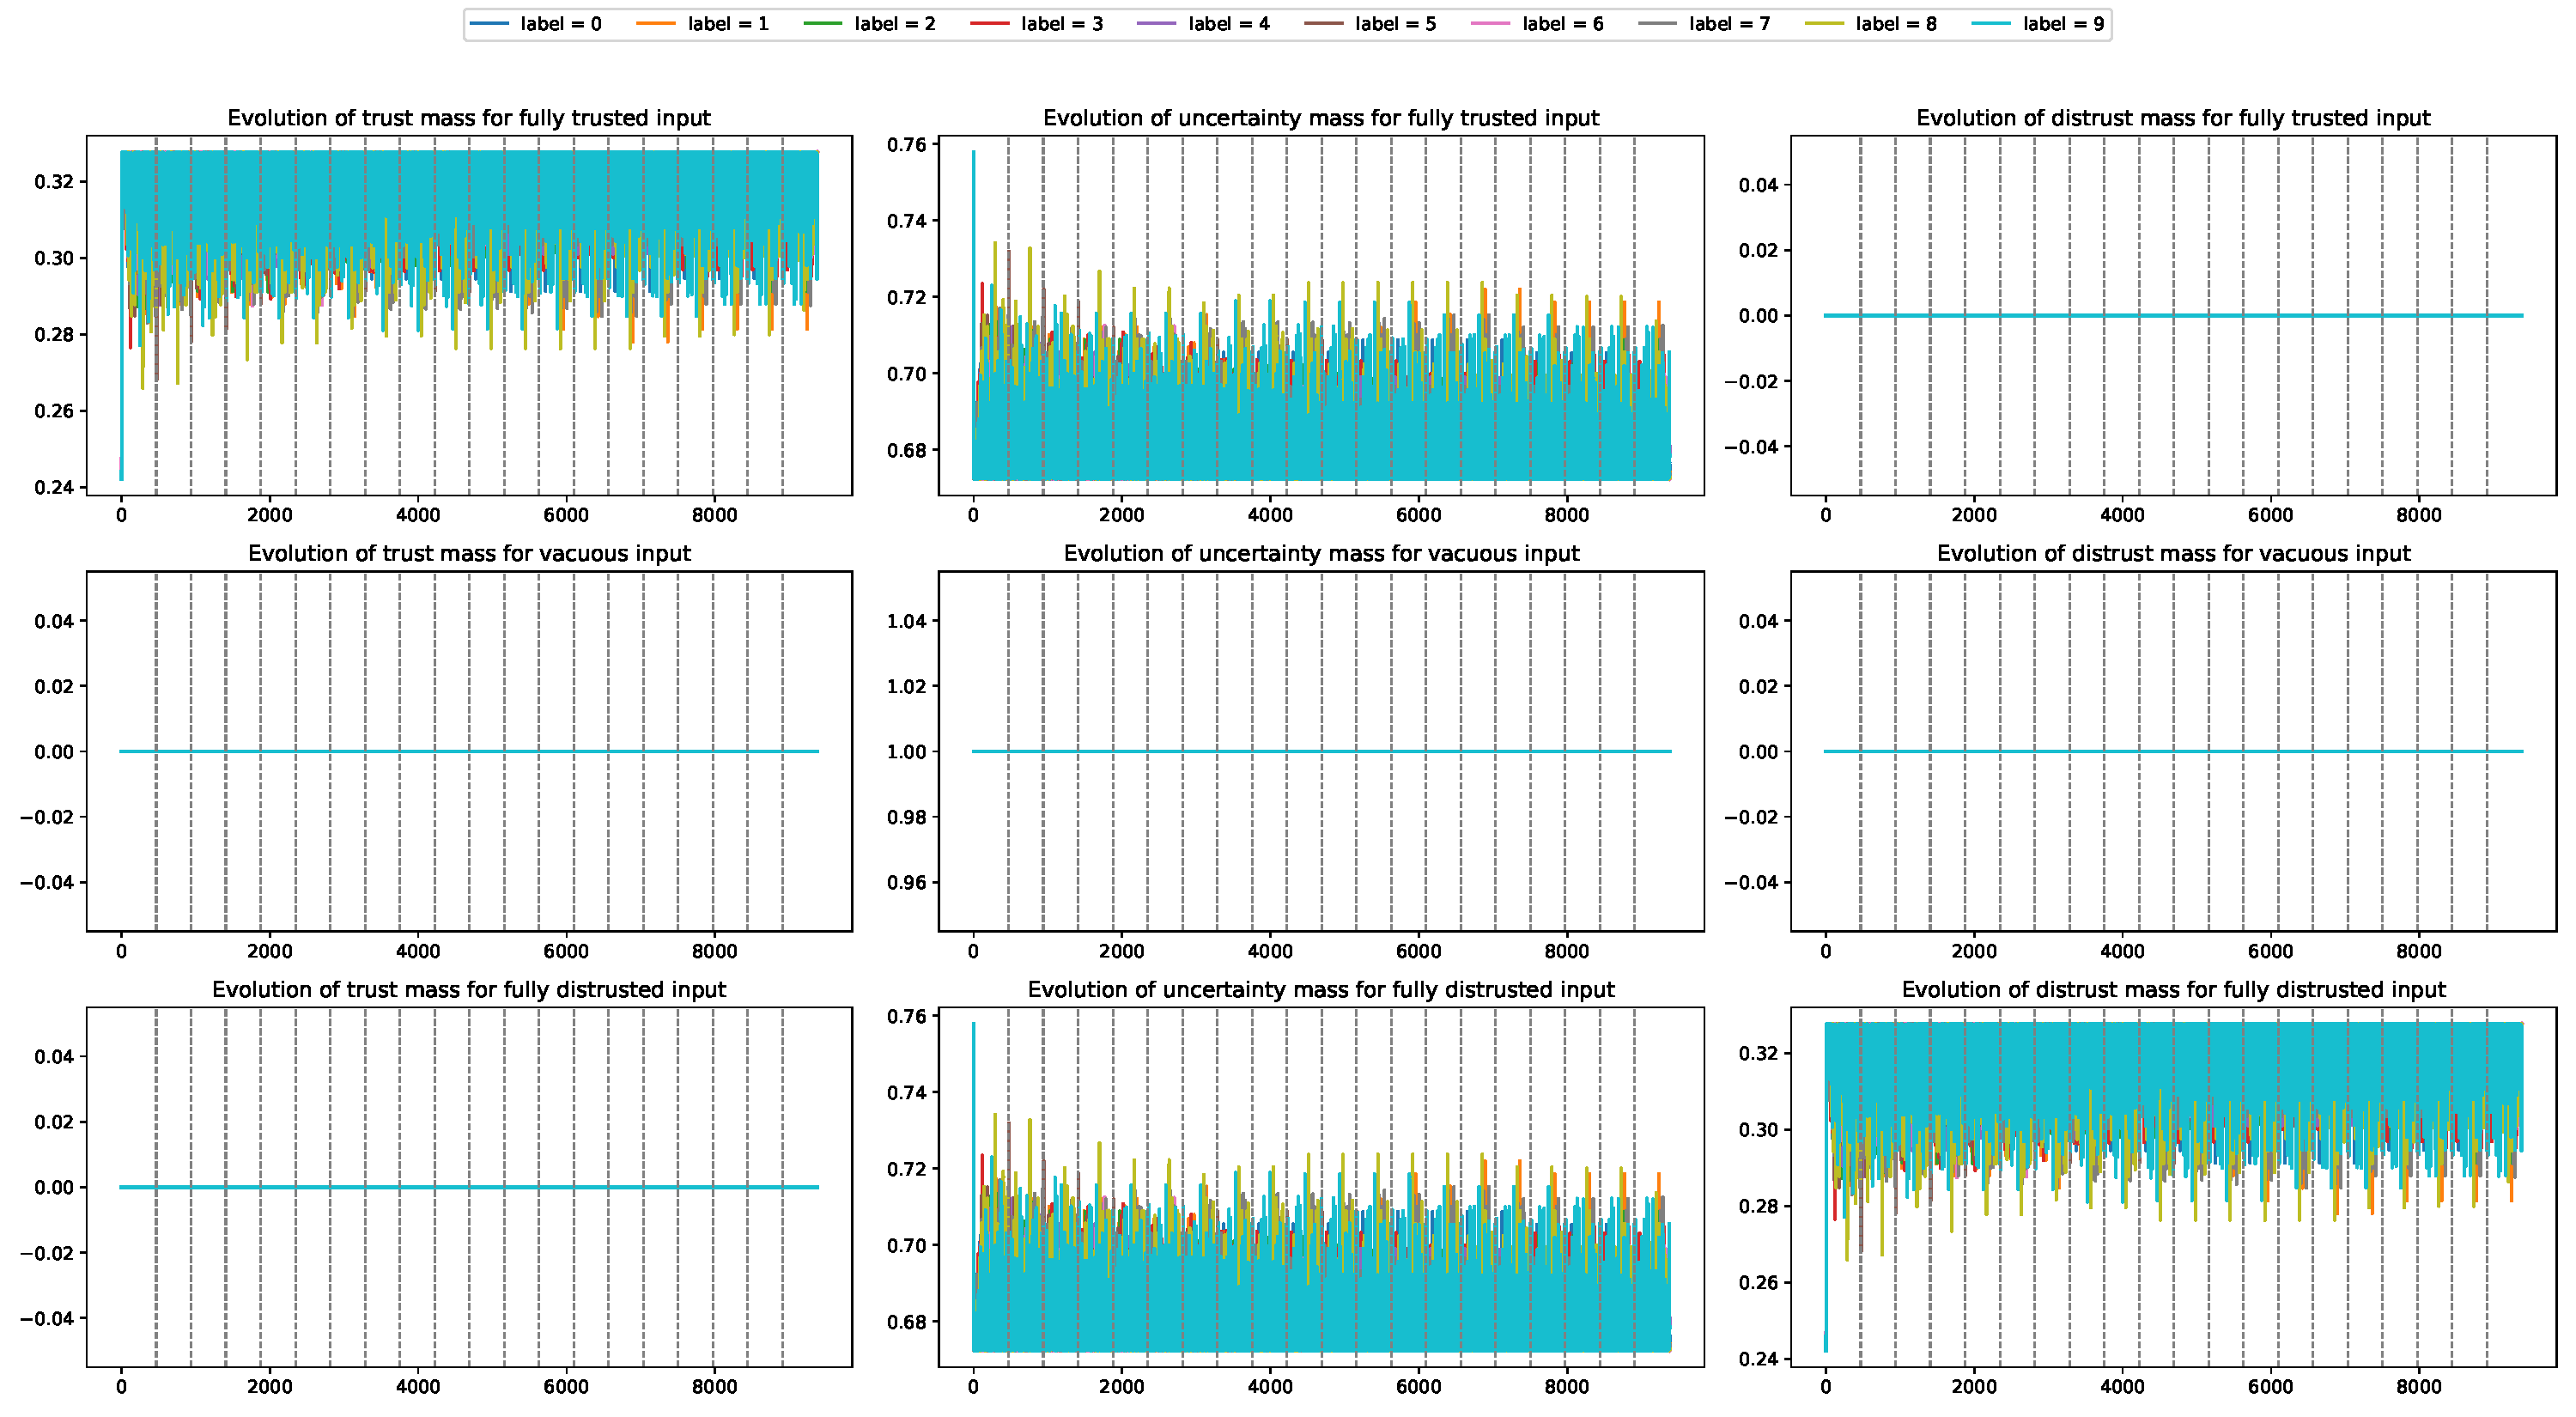
\includegraphics[width=0.8\textwidth]{latex/PTAS_Eval_mnist_32_vacuous_vacuous_eps_0.05_PathSize_None__plot_ptas.pdf}
\caption{mnist\_32\_vacuous\_vacuous, $\varepsilon$=0.05}
\end{figure}

\begin{figure}[htbp]
\centering
  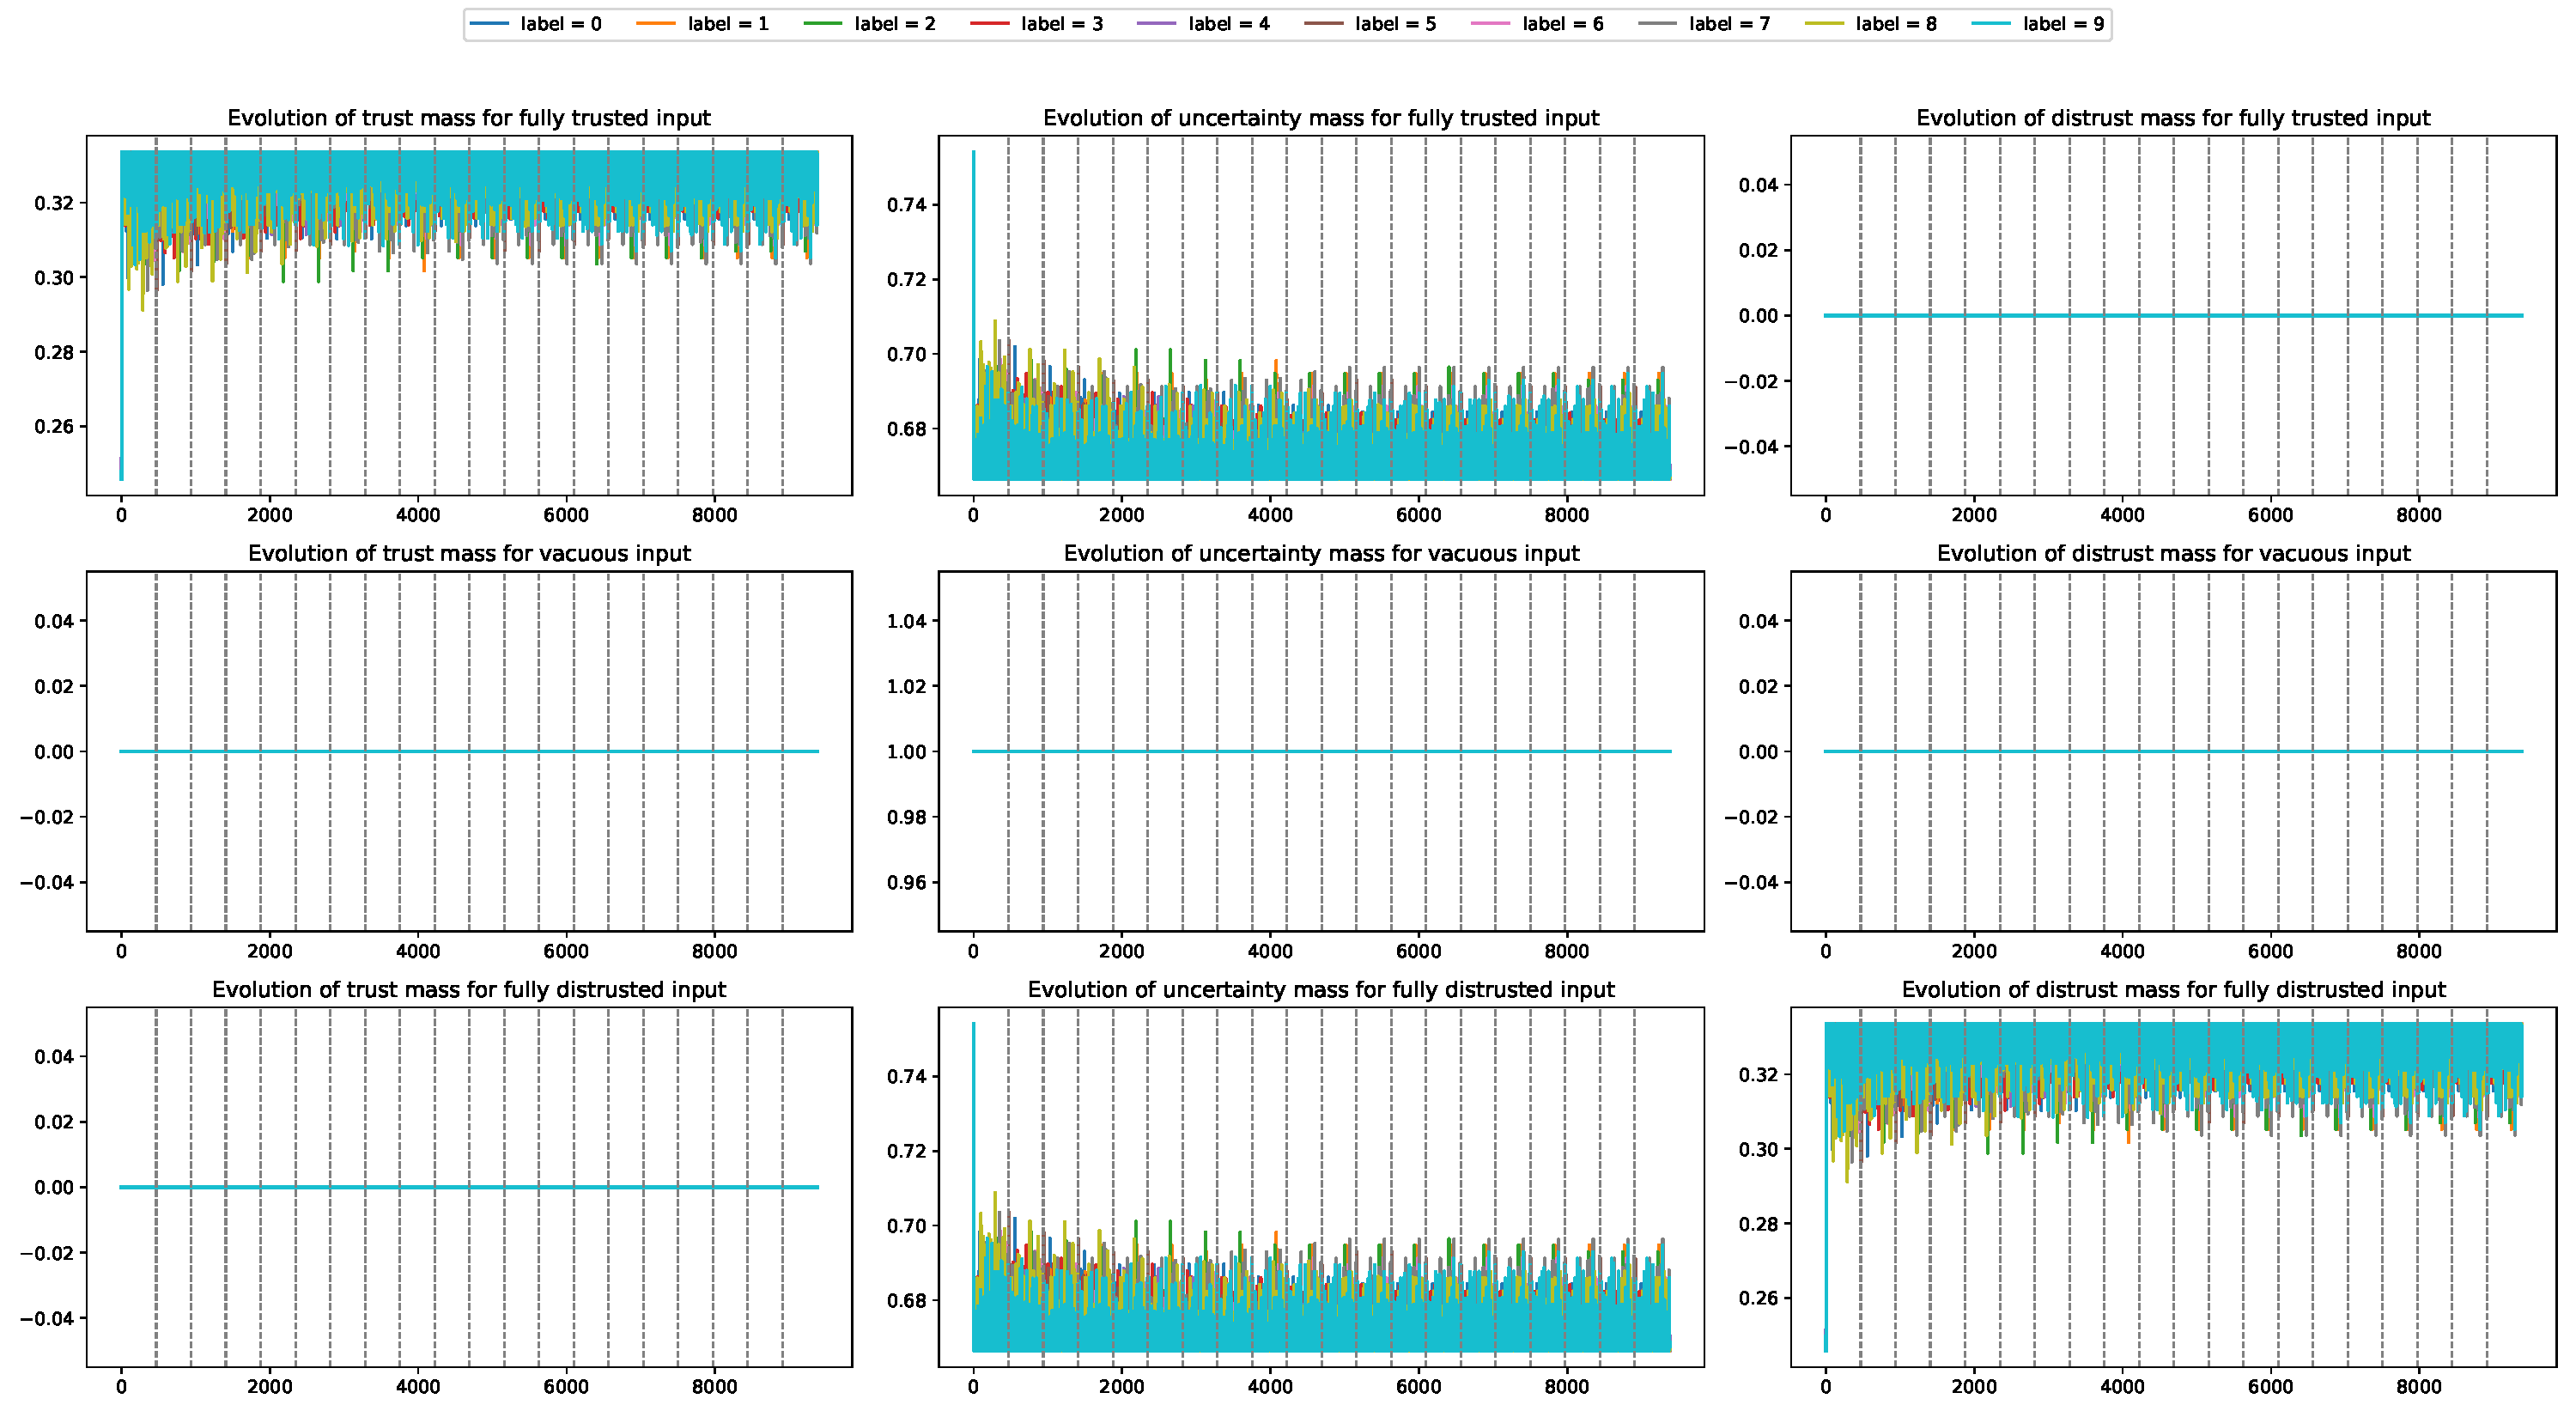
\includegraphics[width=0.8\textwidth]{latex/PTAS_Eval_mnist_64_vacuous_vacuous_eps_0.05_PathSize_None__plot_ptas.pdf}
\caption{mnist\_64\_vacuous\_vacuous, $\varepsilon$=0.05}
\end{figure}

\subsection{\ac{IPTA}}

\begin{figure}[htbp]
\centering
\subfloat[{mnist\_128\_trust\_trust, ps=1}]{%
  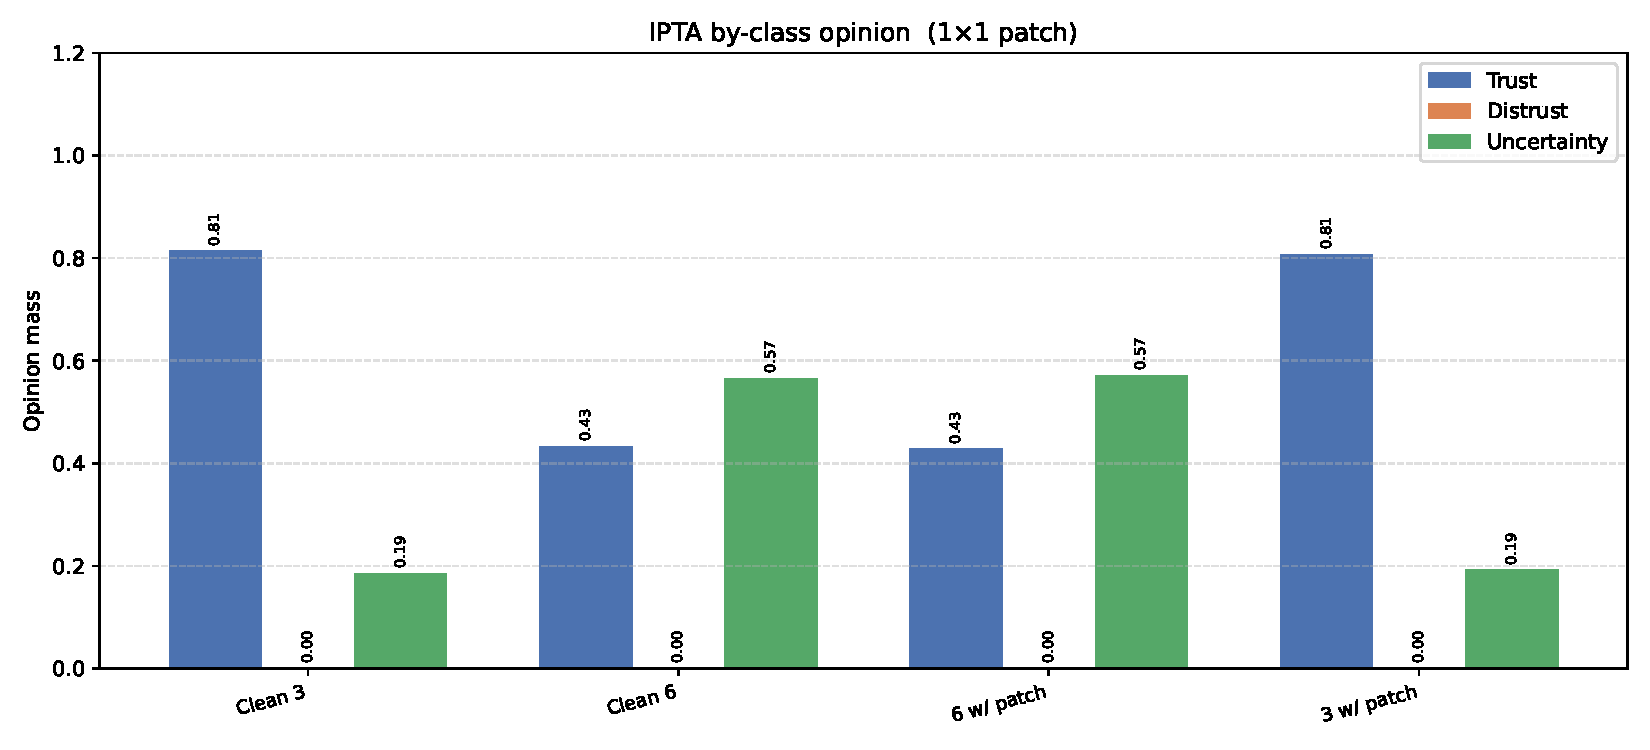
\includegraphics[width=0.3\textwidth]{latex/NN_Train_mnist_128_trust_trust_PathSize_1__ipta_table2a.pdf}%
}
\subfloat[{mnist\_128\_trust\_trust, ps=10}]{%
  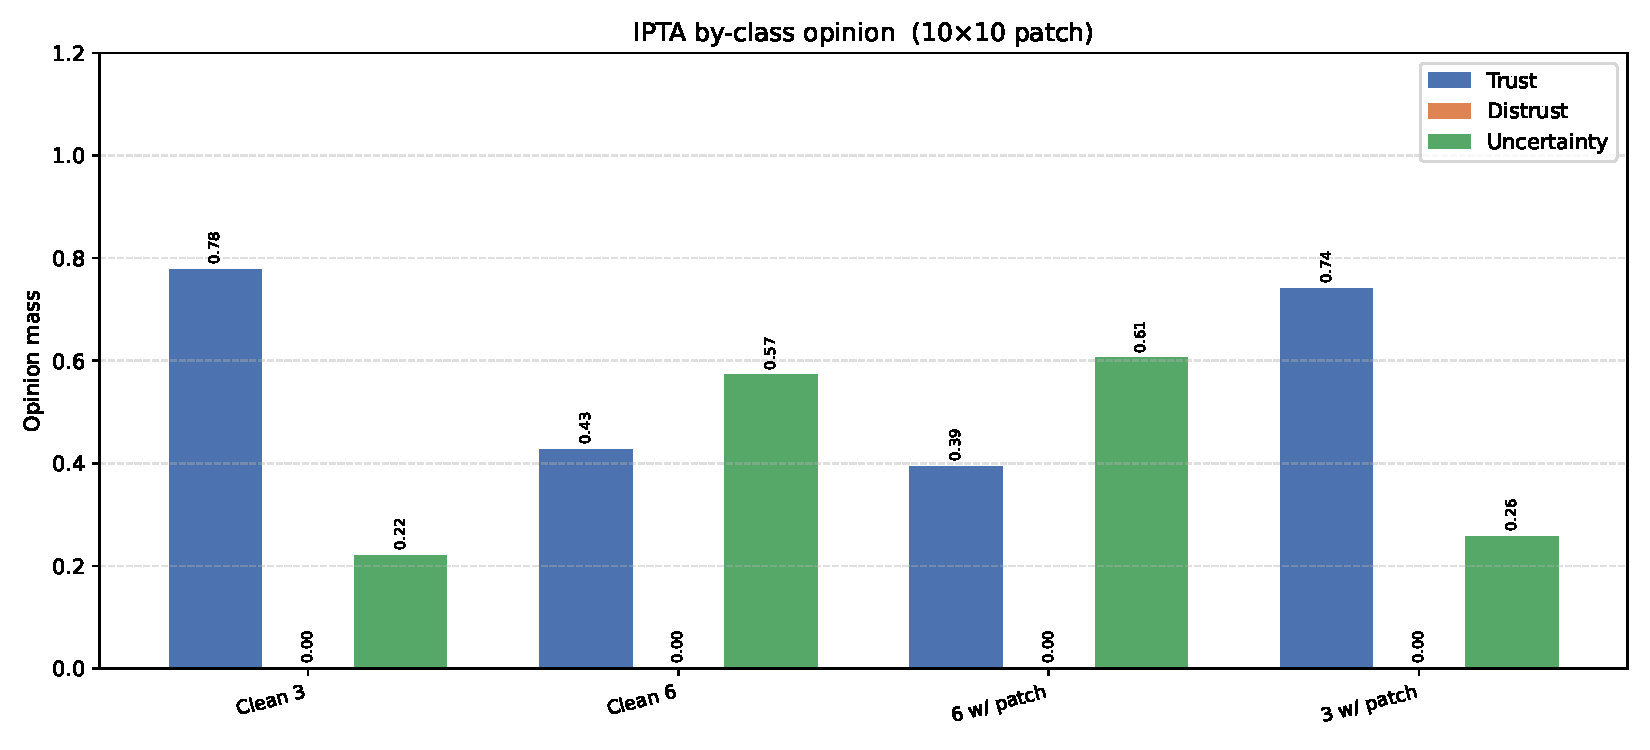
\includegraphics[width=0.3\textwidth]{latex/NN_Train_mnist_128_trust_trust_PathSize_10__ipta_table2a.pdf}%
}
\subfloat[{mnist\_128\_trust\_trust, ps=27}]{%
  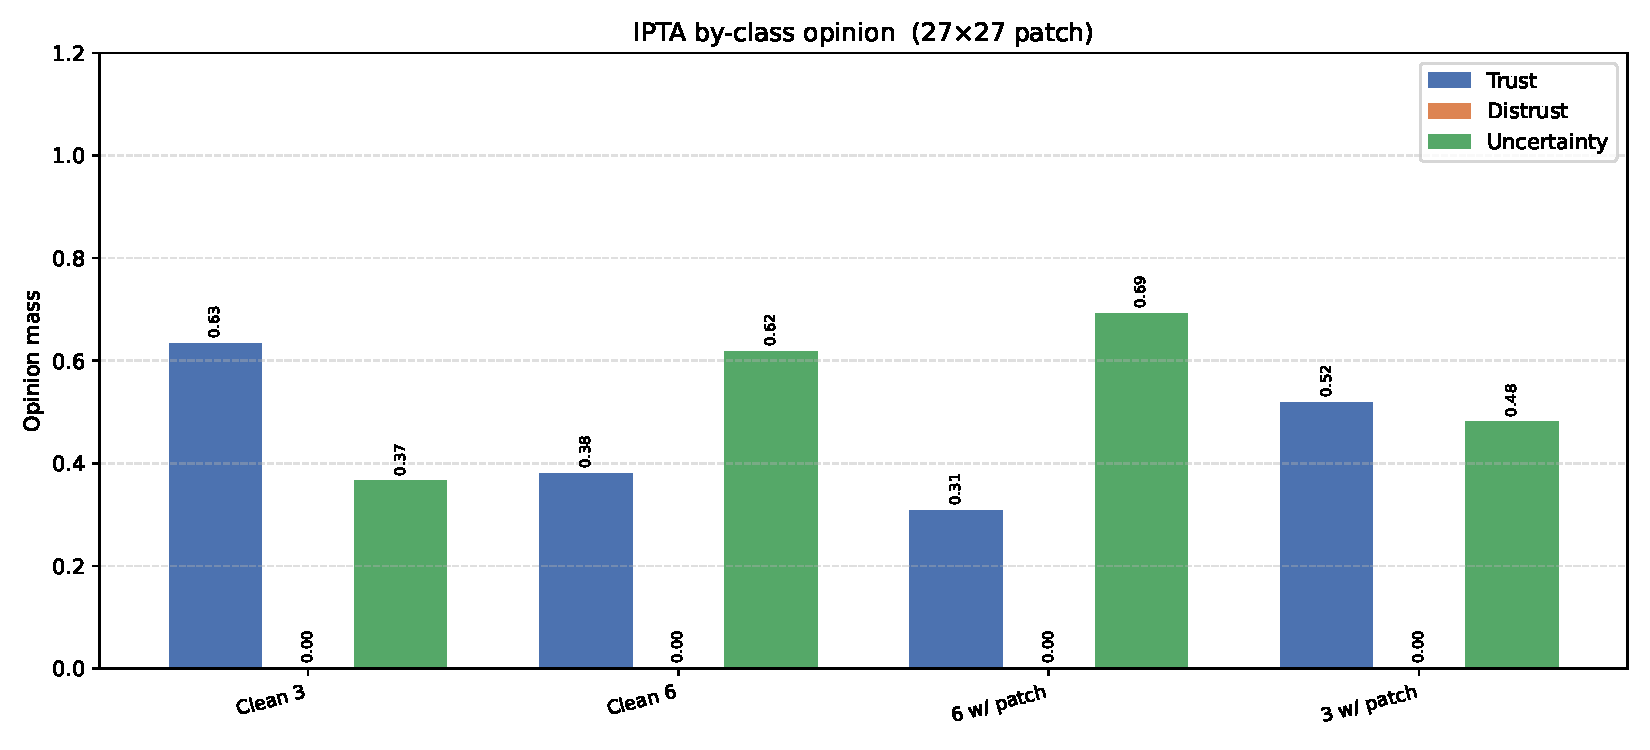
\includegraphics[width=0.3\textwidth]{latex/NN_Train_mnist_128_trust_trust_PathSize_27__ipta_table2a.pdf}%
}
\\
\subfloat[{mnist\_128\_trust\_trust, ps=4}]{%
  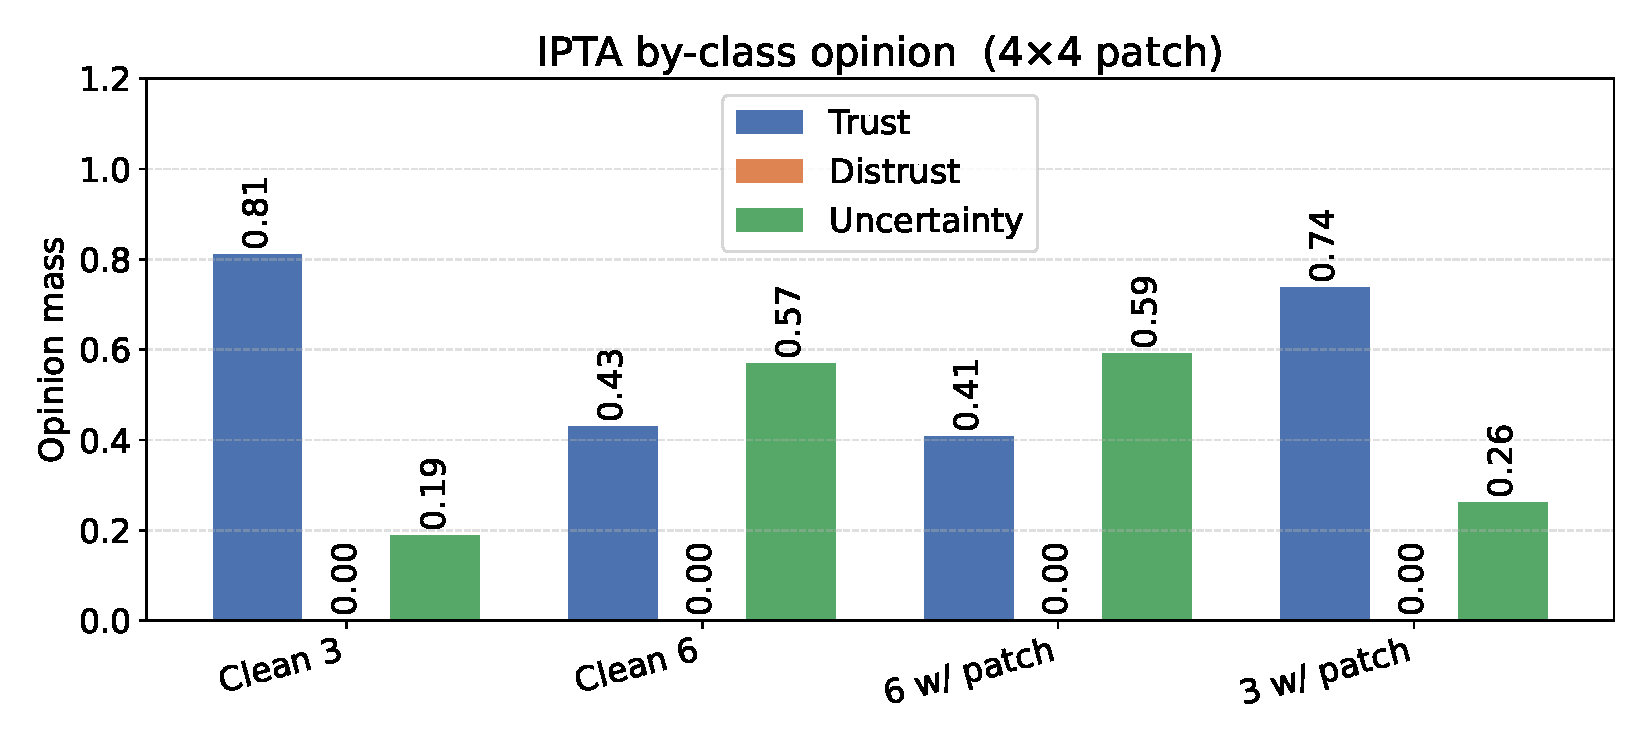
\includegraphics[width=0.3\textwidth]{latex/NN_Train_mnist_128_trust_trust_PathSize_4__ipta_table2a.pdf}%
}
\caption{IPTA -- Table 2a}
\end{figure}


\begin{figure}[htbp]
\centering
\subfloat[{mnist\_128\_trust\_trust, ps=1}]{%
  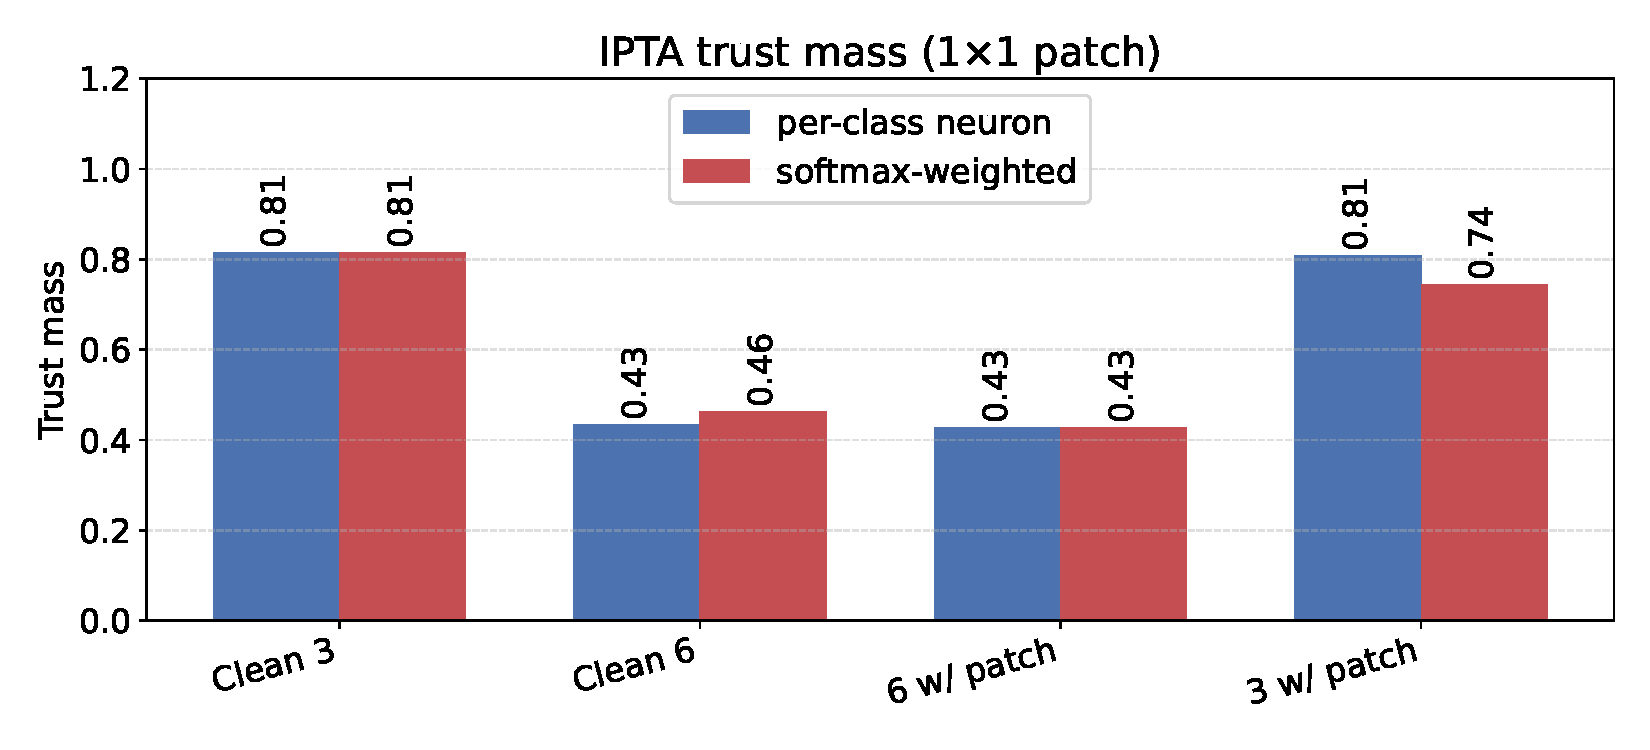
\includegraphics[width=0.3\textwidth]{latex/NN_Train_mnist_128_trust_trust_PathSize_1__ipta_trust_2a_vs_2c.pdf}%
}
\subfloat[{mnist\_128\_trust\_trust, ps=10}]{%
  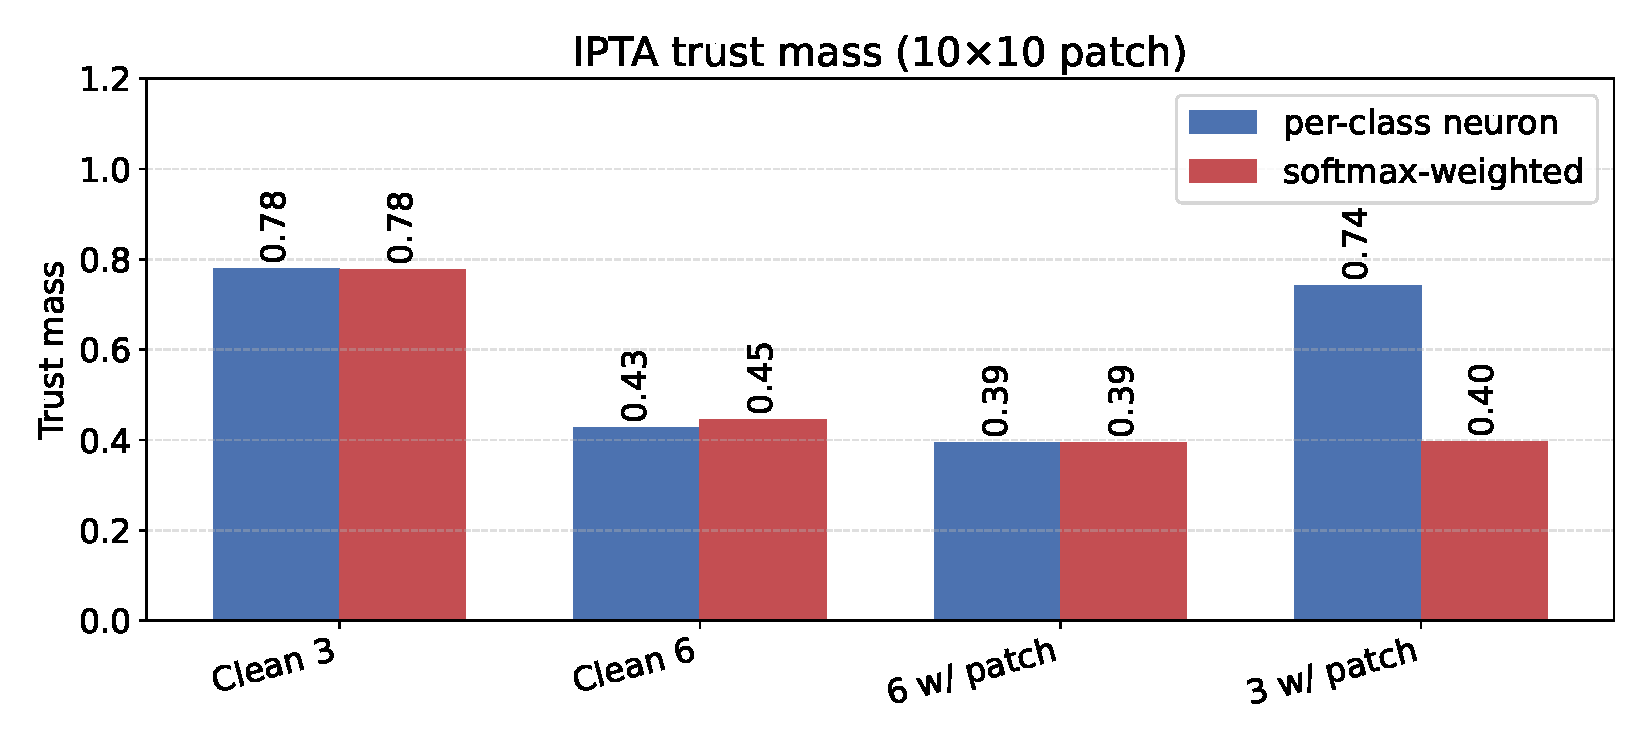
\includegraphics[width=0.3\textwidth]{latex/NN_Train_mnist_128_trust_trust_PathSize_10__ipta_trust_2a_vs_2c.pdf}%
}
\subfloat[{mnist\_128\_trust\_trust, ps=27}]{%
  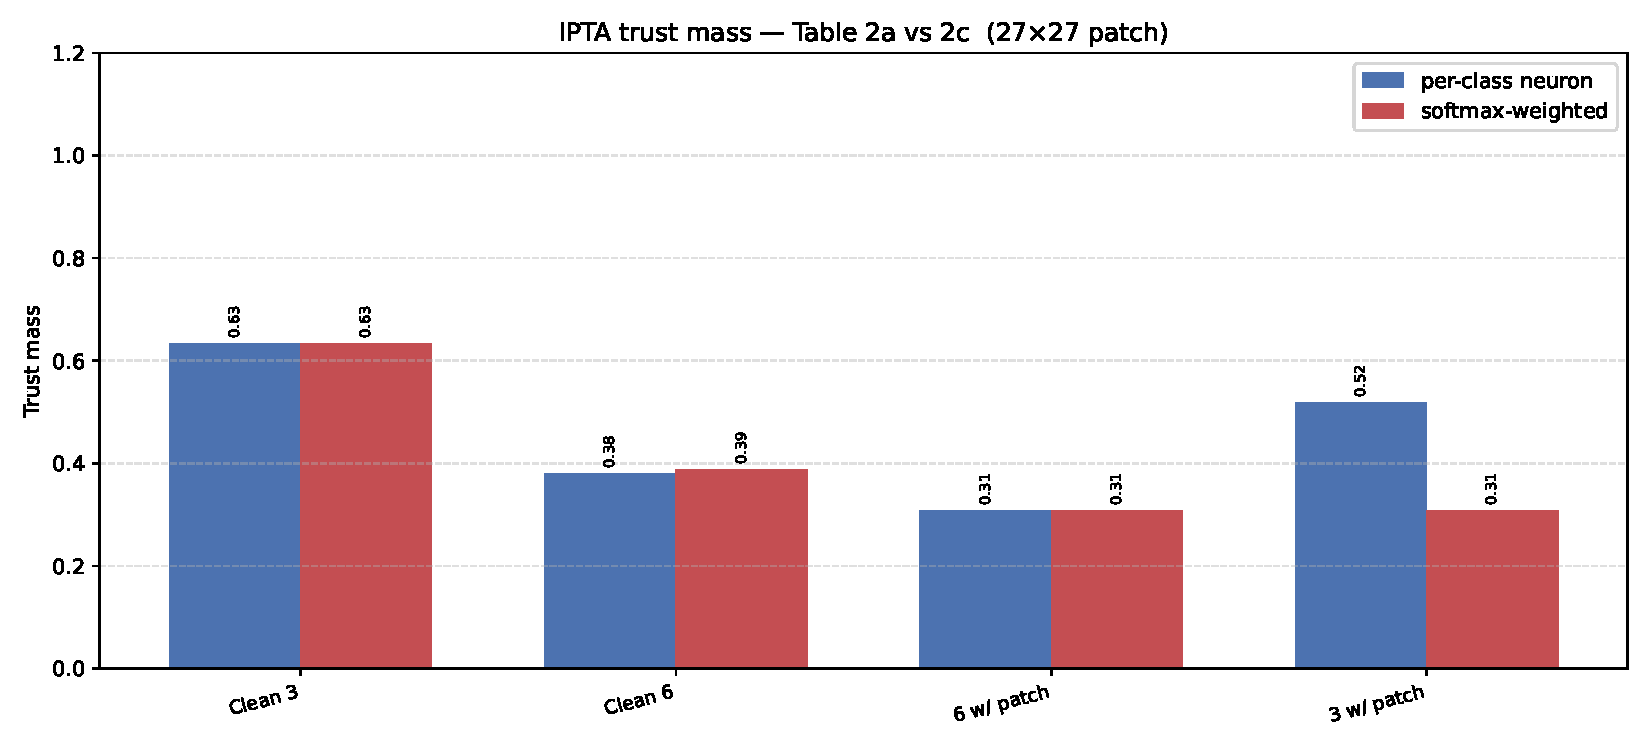
\includegraphics[width=0.3\textwidth]{latex/NN_Train_mnist_128_trust_trust_PathSize_27__ipta_trust_2a_vs_2c.pdf}%
}
\\
\subfloat[{mnist\_128\_trust\_trust, ps=4}]{%
  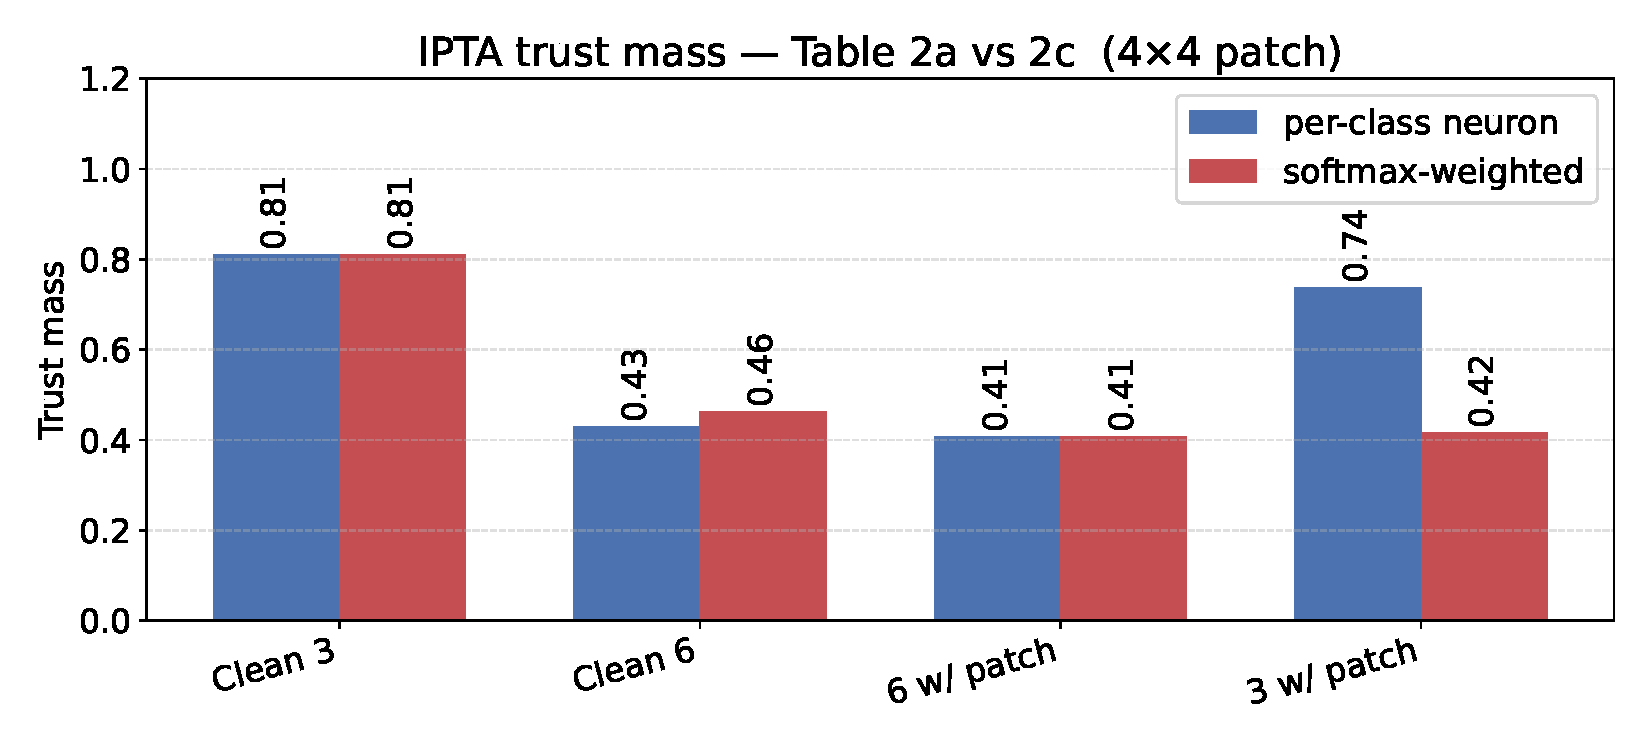
\includegraphics[width=0.3\textwidth]{latex/NN_Train_mnist_128_trust_trust_PathSize_4__ipta_trust_2a_vs_2c.pdf}%
}
\caption{IPTA -- Trust 2a vs 2c}
\end{figure}

\chapter{More results from usecase chapter}
\label{app:noise_analysis}

\section{PaTAS Confidence Signal: Per-Sample Input Trust Feedforward}
\label{sec:per_sample}
This section presents a complementary experiment to \Cref{sec:patas_discriminator}, 
in which the trust feedforward uses per-sample calibrated input trust rather 
than a fully trusted opinion. In the main experiment, the feedforward receives 
a fully trusted input opinion $(1, 0, 0)$ for all samples regardless of their 
actual noise level, isolating the contribution of parameter trust accumulated 
during training. Here, each test sample $i$ instead receives its own calibrated 
input trust opinion $T_{x_i} = \text{feature\_trust}(\sigma_i)$, where $\sigma_i$ 
is the actual noise level drawn for that sample, so that both input quality 
and parameter trust contribute jointly to the output opinion.

\Cref{fig:patas_persample} visualizes the resulting opinion masses and 
discriminative gaps.

\begin{figure}[p]
\centering
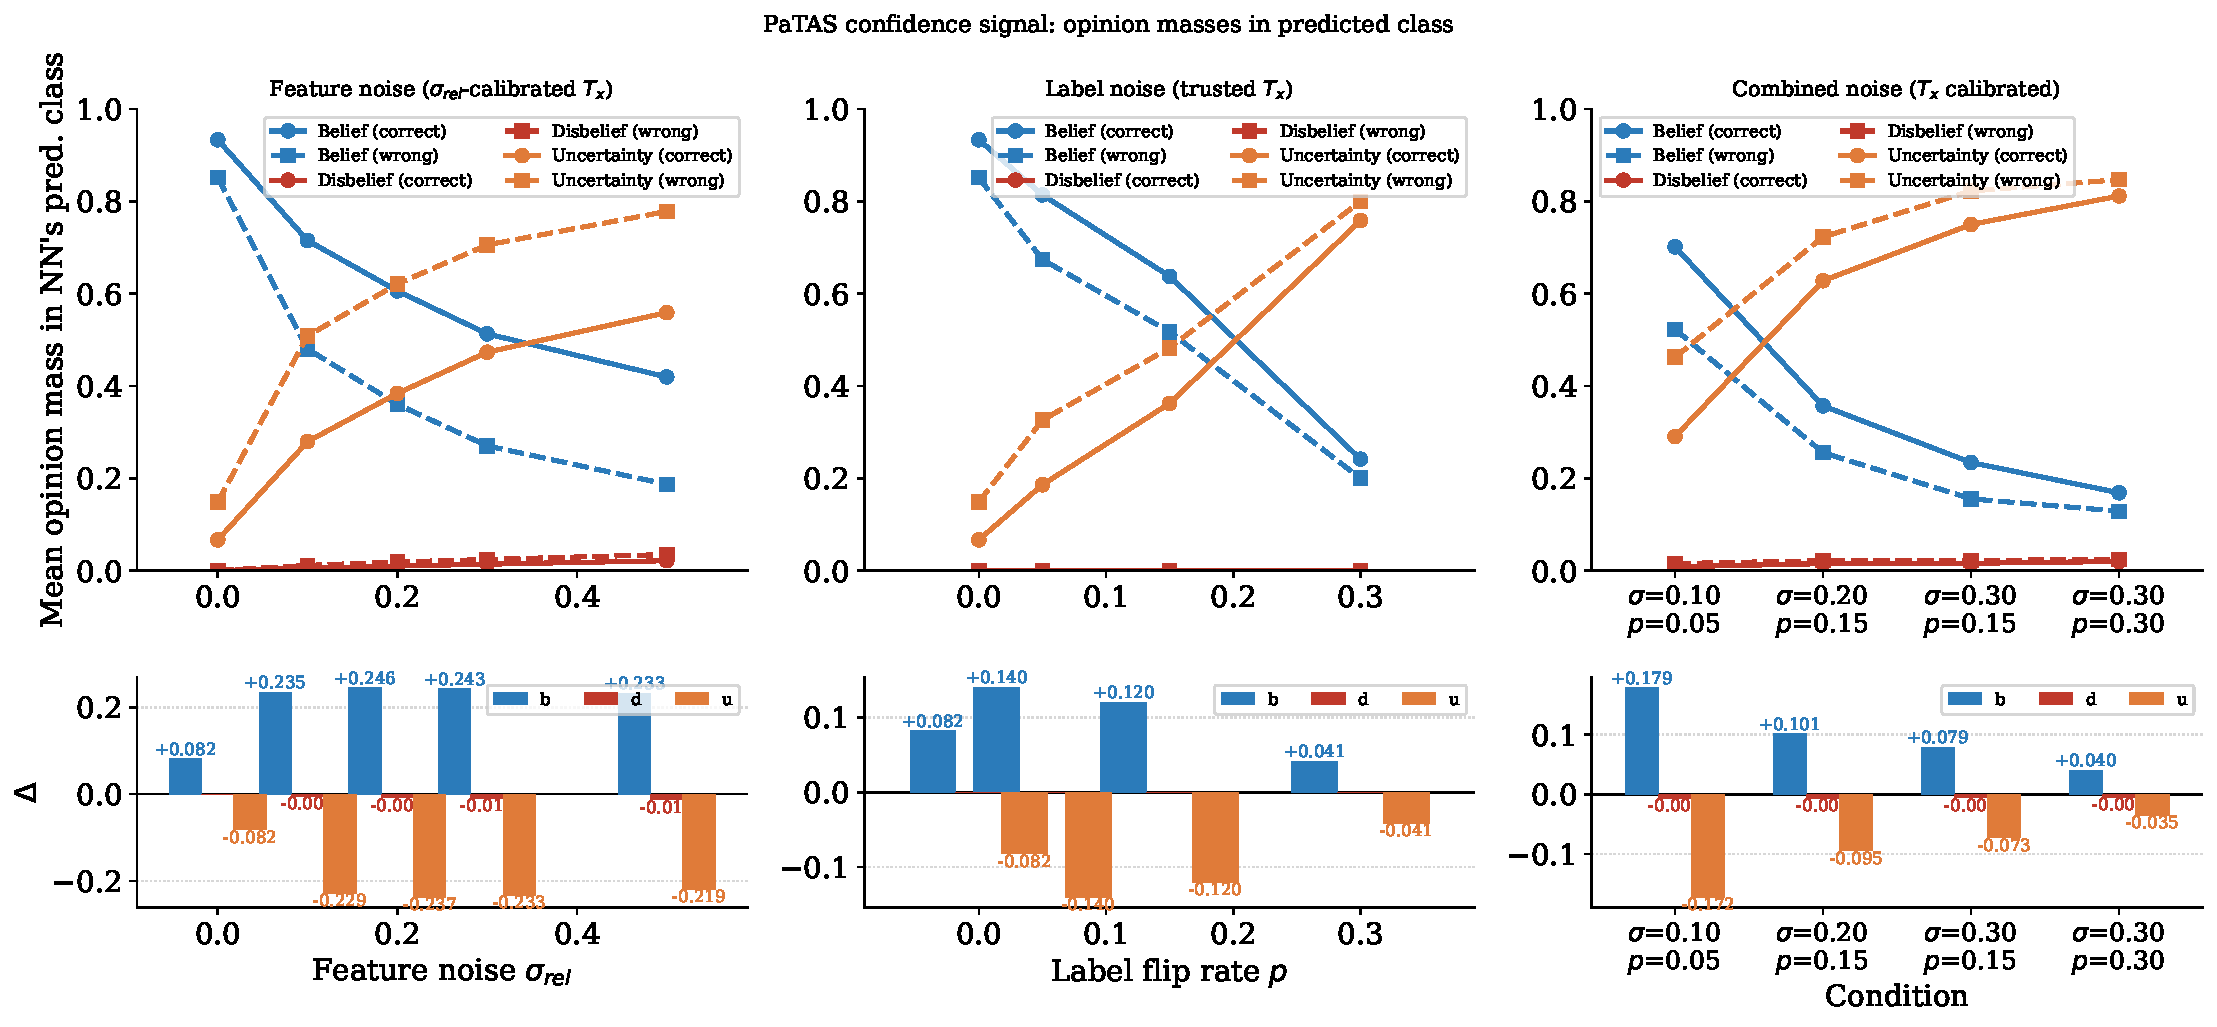
\includegraphics[width=\textwidth]{img/usecase/patas_effectiveness_agg_per_sample.pdf}
\caption{\ac{PaTAS} opinion masses with per-sample calibrated input trust 
feedforward. Top: mean opinion values for correctly-classified (solid lines, 
circles) versus misclassified (dashed lines, squares) samples. Bottom: 
$\Delta = \text{correct} - \text{wrong}$, showing the discriminative gap 
per component. Left: feature noise. Center: label noise. Right: combined 
noise.}
\label{fig:patas_persample}
\end{figure}

Three observations distinguish this experiment from the main results of 
\Cref{sec:patas_discriminator}.

\paragraph{Disbelief is no longer zero under feature noise.}
When per-sample input trust is fed forward, disbelief becomes a small but 
non-negligible component of the discriminative signal under feature noise: 
$\Delta d$ ranges from $-0.006$ at $\sigma_{\text{rel}} = 0.10$ to $-0.013$ 
at $\sigma_{\text{rel}} = 0.50$. This is consistent with the trust 
quantification design: the feature trust opinion assigns a small disbelief 
component $d = \sigma_{\text{rel}}(1 - u)$ to each sample, and this 
propagates through the \ac{TNN} to produce a non-zero disbelief in the 
output opinion. The effect is small relative to the belief and uncertainty 
gaps, but it confirms that the disbelief channel carries meaningful 
provenance information when input quality is explicitly encoded.

\paragraph{The discriminative gap $\Delta b$ is larger than in the 
fully-trusted case.}
Under feature noise, $\Delta b$ ranges from $+0.235$ at 
$\sigma_{\text{rel}} = 0.10$ to $+0.243$ at $\sigma_{\text{rel}} = 0.20$, 
slightly higher than the corresponding values of $+0.228$ and $+0.237$ in 
the main experiment. This reflects the additional discriminative power 
contributed by the per-sample input trust: samples with lower noise receive 
higher input belief, which amplifies the output belief gap between correct 
and incorrect predictions. Under label noise the values are identical to 
the main experiment, as expected: the label noise experiment uses fully 
trusted feature inputs in both settings.

\paragraph{The combined noise results show non-zero disbelief gaps.}
Under combined noise, $\Delta d$ is small but consistently negative 
(ranging from $-0.005$ to $-0.007$), confirming that when both feature 
and label corruption are present and input trust is calibrated per sample, 
the disbelief channel contributes a weak additional discriminative signal 
beyond what belief and uncertainty alone provide.

Together, these results confirm that per-sample input trust feedforward 
produces a richer and marginally more discriminative trust signal than the 
fully-trusted baseline, at the cost of requiring knowledge of the per-sample 
noise level $\sigma_i$ at test time. In deployment settings where this 
information is available (for instance, from sensor quality metadata), 
the per-sample variant is preferred. Where it is not, the fully-trusted 
feedforward of \Cref{sec:patas_discriminator} provides a conservative 
but still informative trust signal.


\section{Extended Coverage--Accuracy and ROC Analysis for Selective Prediction}
\label{app:coverage_roc}
 
\Cref{sec:selective_prediction} summarizes the coverage--accuracy
trade-off between \ac{PaTAS} and softmax filtering at representative
operating points (e.g., accuracy at 20\% coverage). This appendix
presents the complete curves for all four panels of each noise axis,
together with the corresponding ROC curve and AUC for each condition,
obtained by treating the filtering score (\ac{PaTAS} projected
probability $\pi = b + u/2$, or the softmax maximum probability) as a
ranking signal and correctness of the \ac{NN}'s prediction as the
binary outcome.
 
\subsection{Feature Noise}
\label{app:coverage_roc_feature}
 
\begin{figure}[h]
\centering
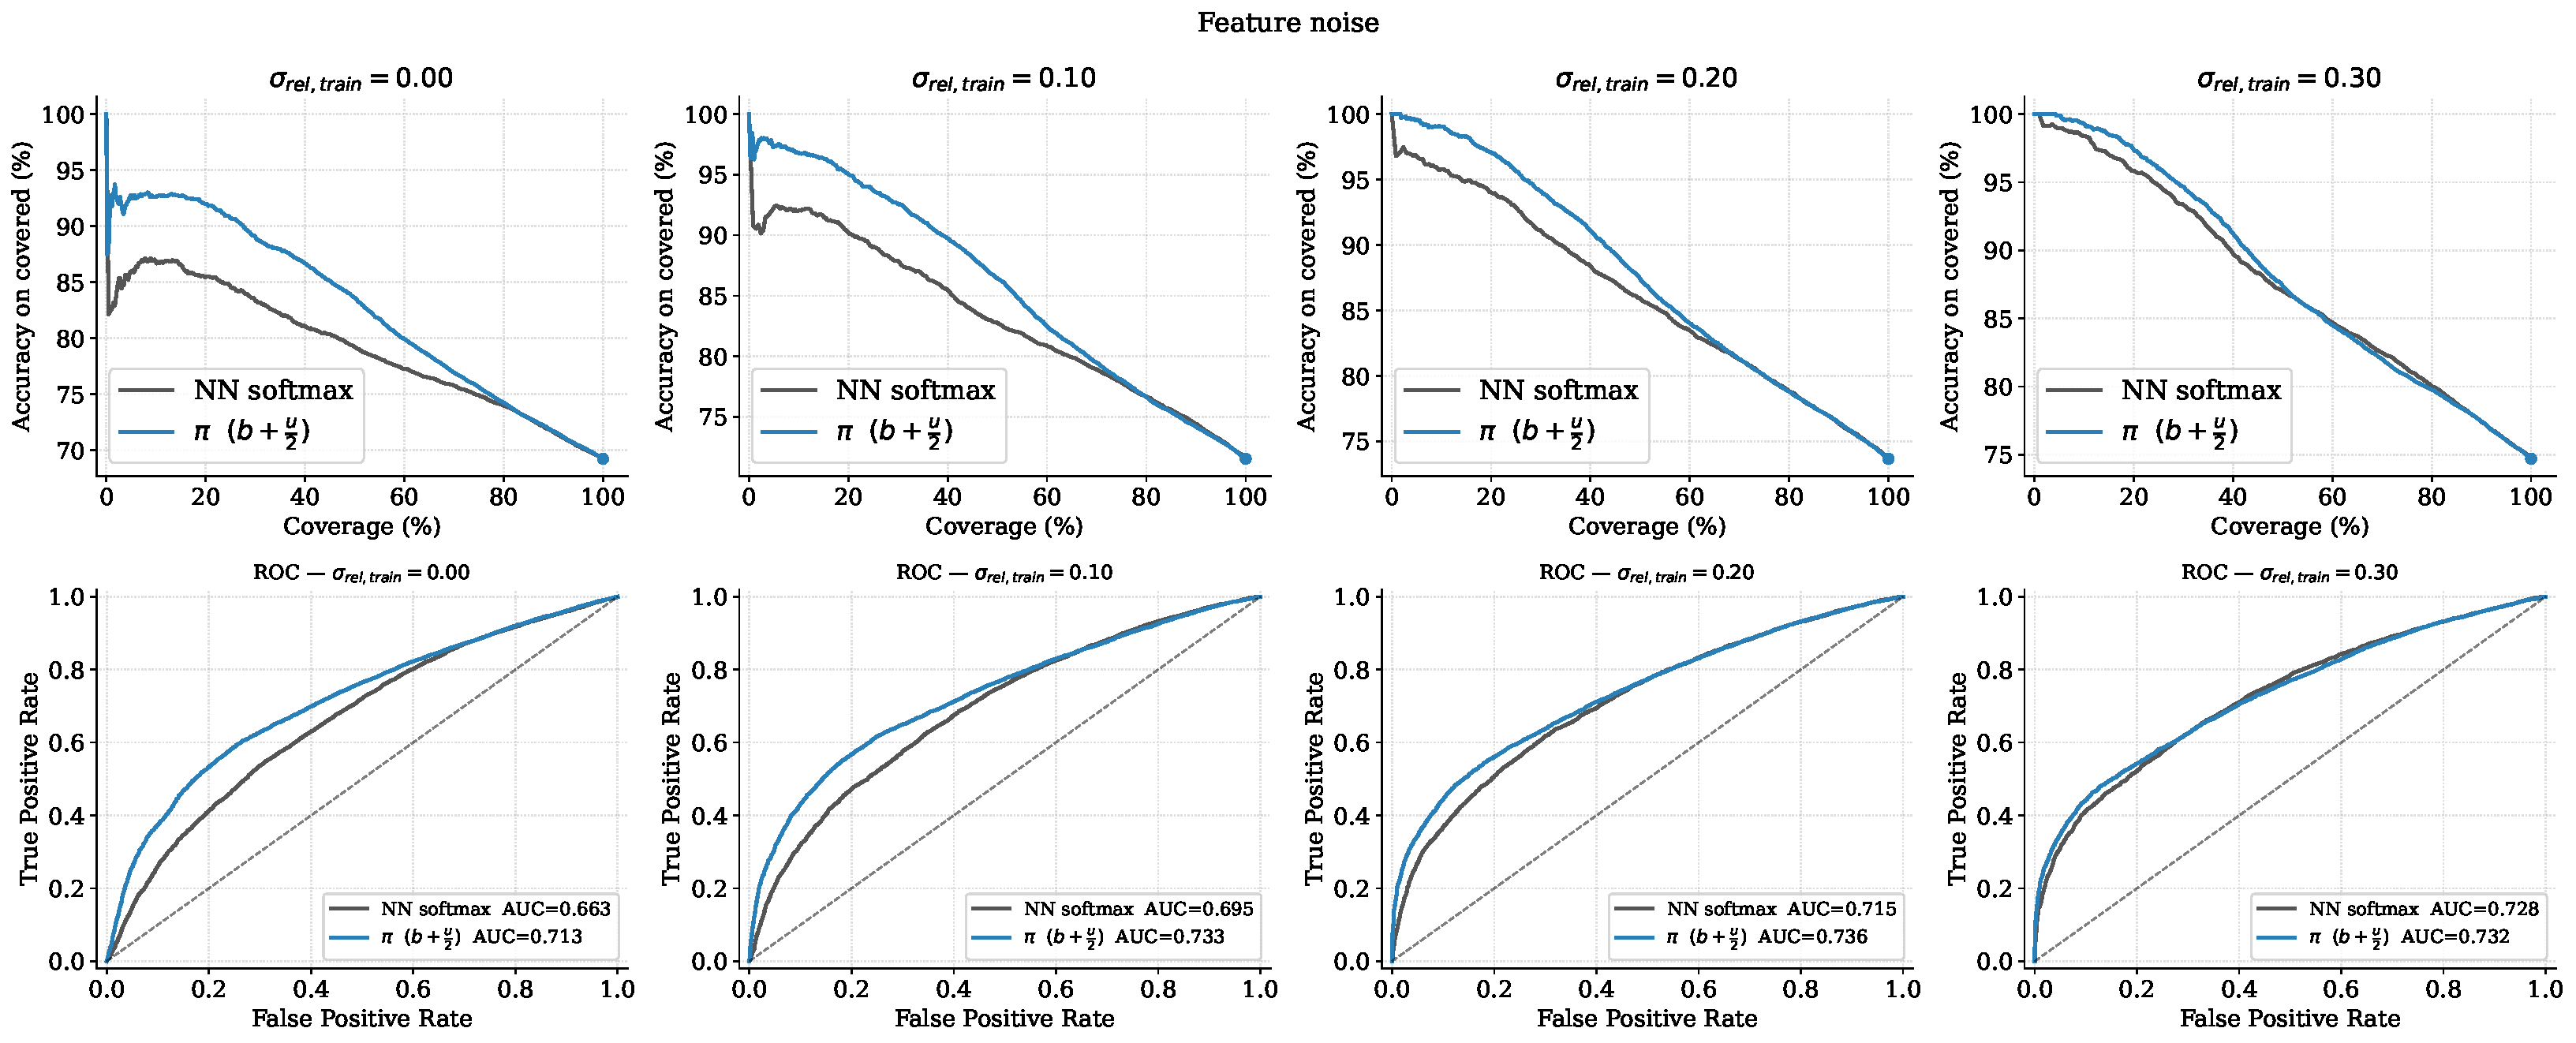
\includegraphics[width=\linewidth]{img/usecase/app/coverage_accuracy_feature.pdf}
\caption{Top: coverage--accuracy curves under feature noise, extending
\Cref{fig:coverage_accuracy_feature}, for
$\sigma_{\text{rel,train}} \in \{0.00, 0.10, 0.20, 0.30\}$ with test
noise $\sigma_{\text{rel,test}} \sim \text{Uniform}(0,1)$. Bottom:
corresponding ROC curves and AUC for \ac{PaTAS} ($\pi = b + u/2$)
versus softmax maximum probability.}
\label{fig:app_coverage_roc_feature}
\end{figure}
 
\Cref{fig:app_coverage_roc_feature} confirms the coverage--accuracy
advantage reported in \Cref{sec:selective_prediction} at the level of
overall ranking quality. \ac{PaTAS} attains a higher AUC than softmax
at every training noise level: $0.713$ versus $0.663$ at
$\sigma_{\text{rel,train}} = 0.00$, $0.733$ versus $0.695$ at
$\sigma_{\text{rel,train}} = 0.10$, and $0.736$ versus $0.715$ at
$\sigma_{\text{rel,train}} = 0.20$. The gap narrows as training noise
increases, reaching near-parity at $\sigma_{\text{rel,train}} = 0.30$
($0.732$ versus $0.728$), consistent with the convergence of the two
coverage--accuracy curves at higher training noise discussed in
\Cref{sec:selective_prediction} and with the regularization effect of
input noise during training.
 
\subsection{Label Flipping}
\label{app:coverage_roc_label}
 
\begin{figure}[h]
\centering
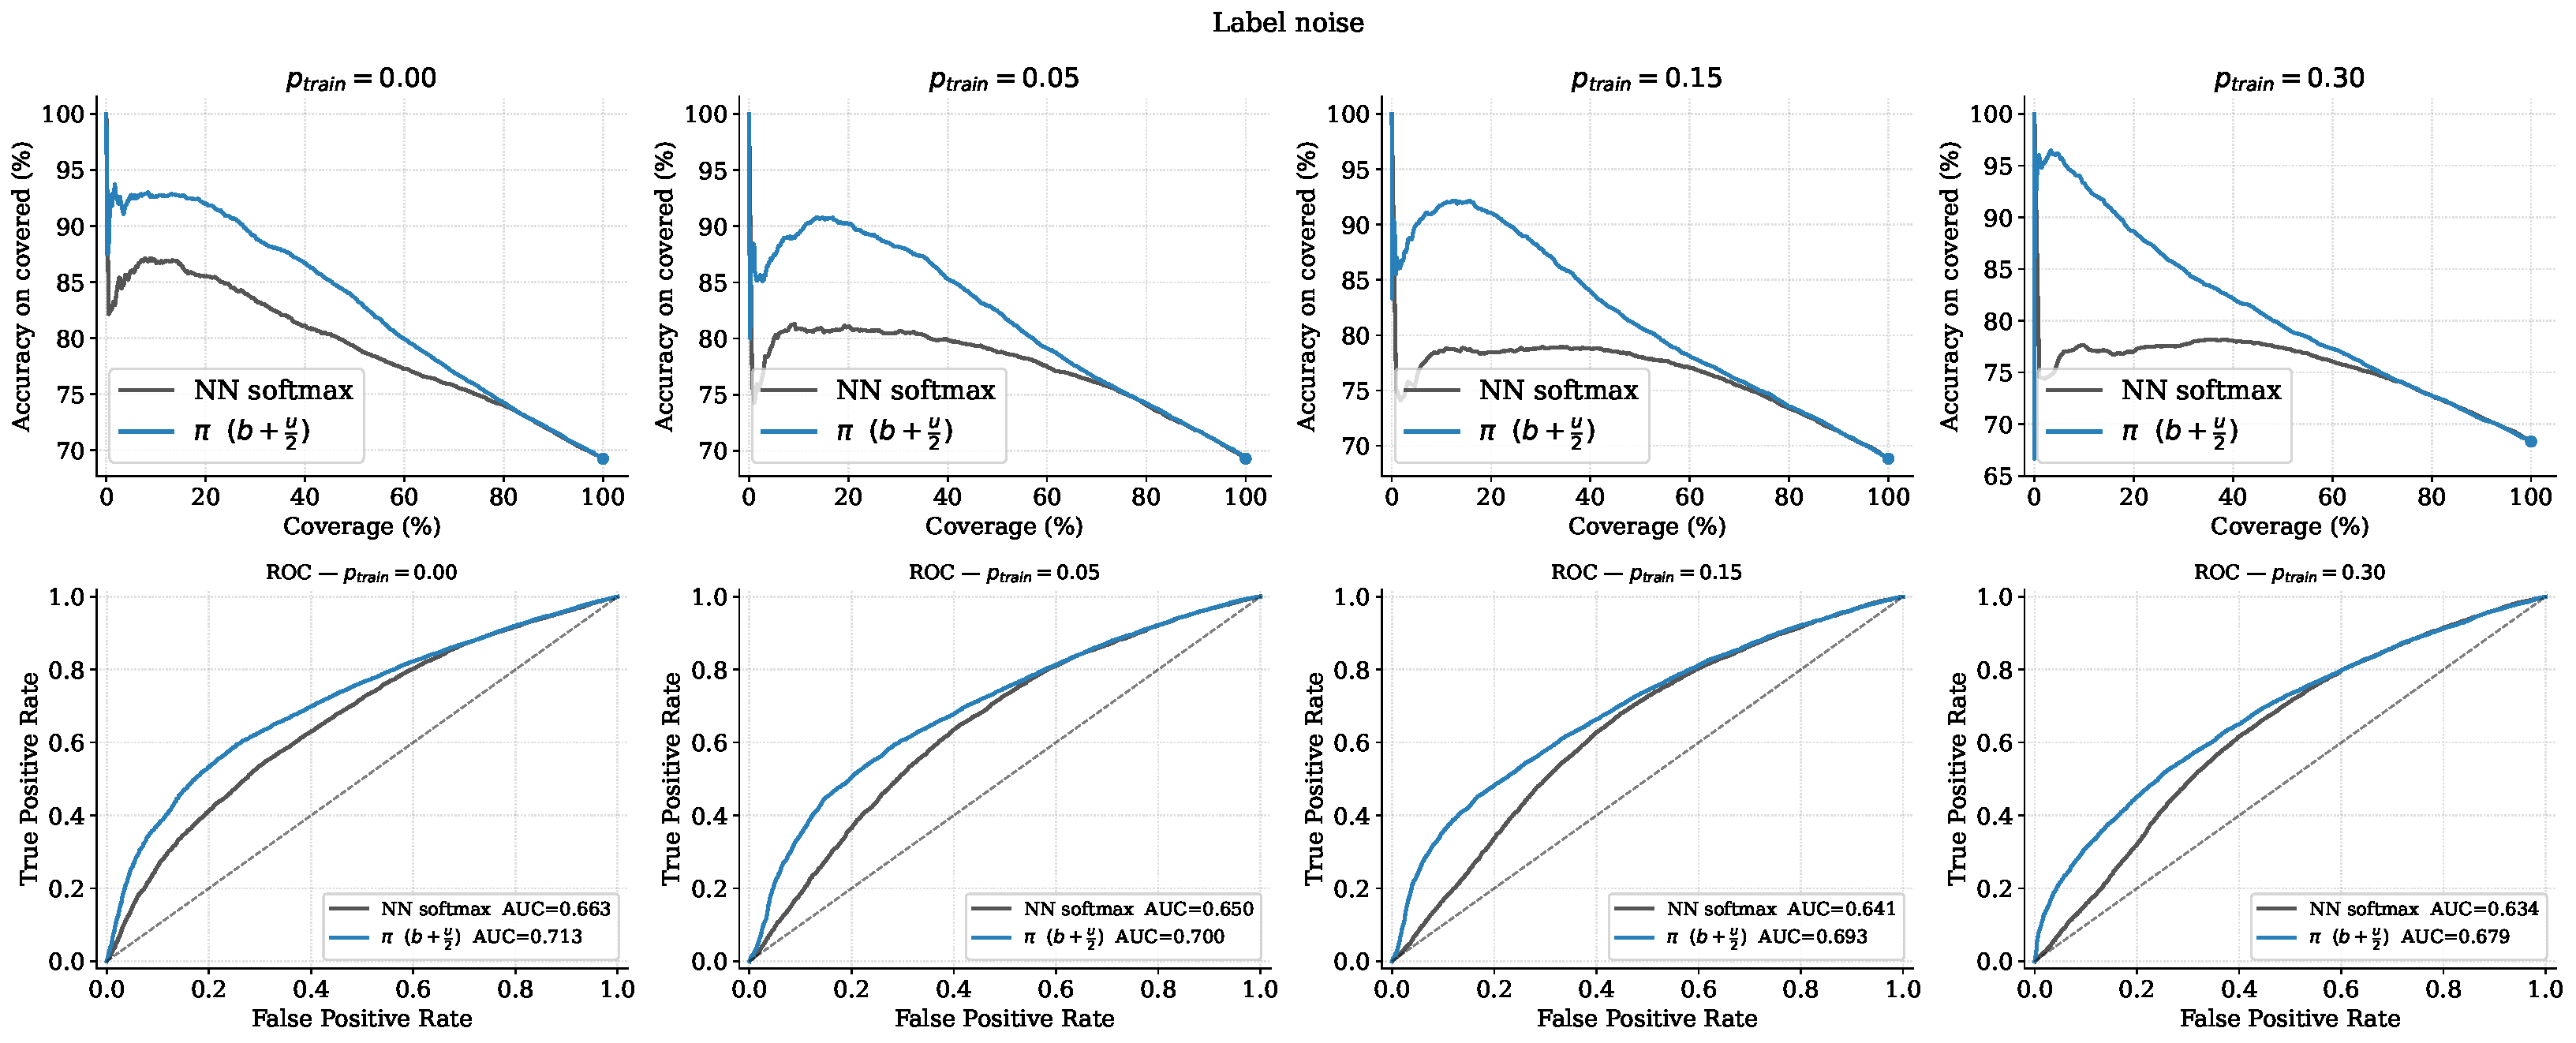
\includegraphics[width=\linewidth]{img/usecase/app/coverage_accuracy_label.pdf}
\caption{Top: coverage--accuracy curves under label flipping, extending
\Cref{fig:coverage_accuracy_label}, for
$p_{\text{train}} \in \{0.00, 0.05, 0.15, 0.30\}$. Bottom: corresponding
ROC curves and AUC for \ac{PaTAS} versus softmax.}
\label{fig:app_coverage_roc_label}
\end{figure}
 
Under label flipping, the AUC advantage of \ac{PaTAS} over softmax is
essentially constant across the evaluated flip rates: $+0.050$ at
$p_{\text{train}} = 0.00$ ($0.713$ vs.\ $0.663$), $+0.050$ at
$p_{\text{train}} = 0.05$ ($0.700$ vs.\ $0.650$), $+0.052$ at
$p_{\text{train}} = 0.15$ ($0.693$ vs.\ $0.641$), and $+0.045$ at
$p_{\text{train}} = 0.30$ ($0.679$ vs.\ $0.634$). Unlike the
feature-noise case, the gap does not narrow with increasing corruption,
mirroring the sustained advantage observed in the coverage--accuracy
curves of \Cref{sec:selective_prediction} and reinforcing the
conclusion that \ac{PaTAS} retains discriminative power under label
corruption even as the absolute AUC of both filters declines.
 
\subsection{Combined Noise}
\label{app:coverage_roc_combined}
 
\begin{figure}[h]
\centering
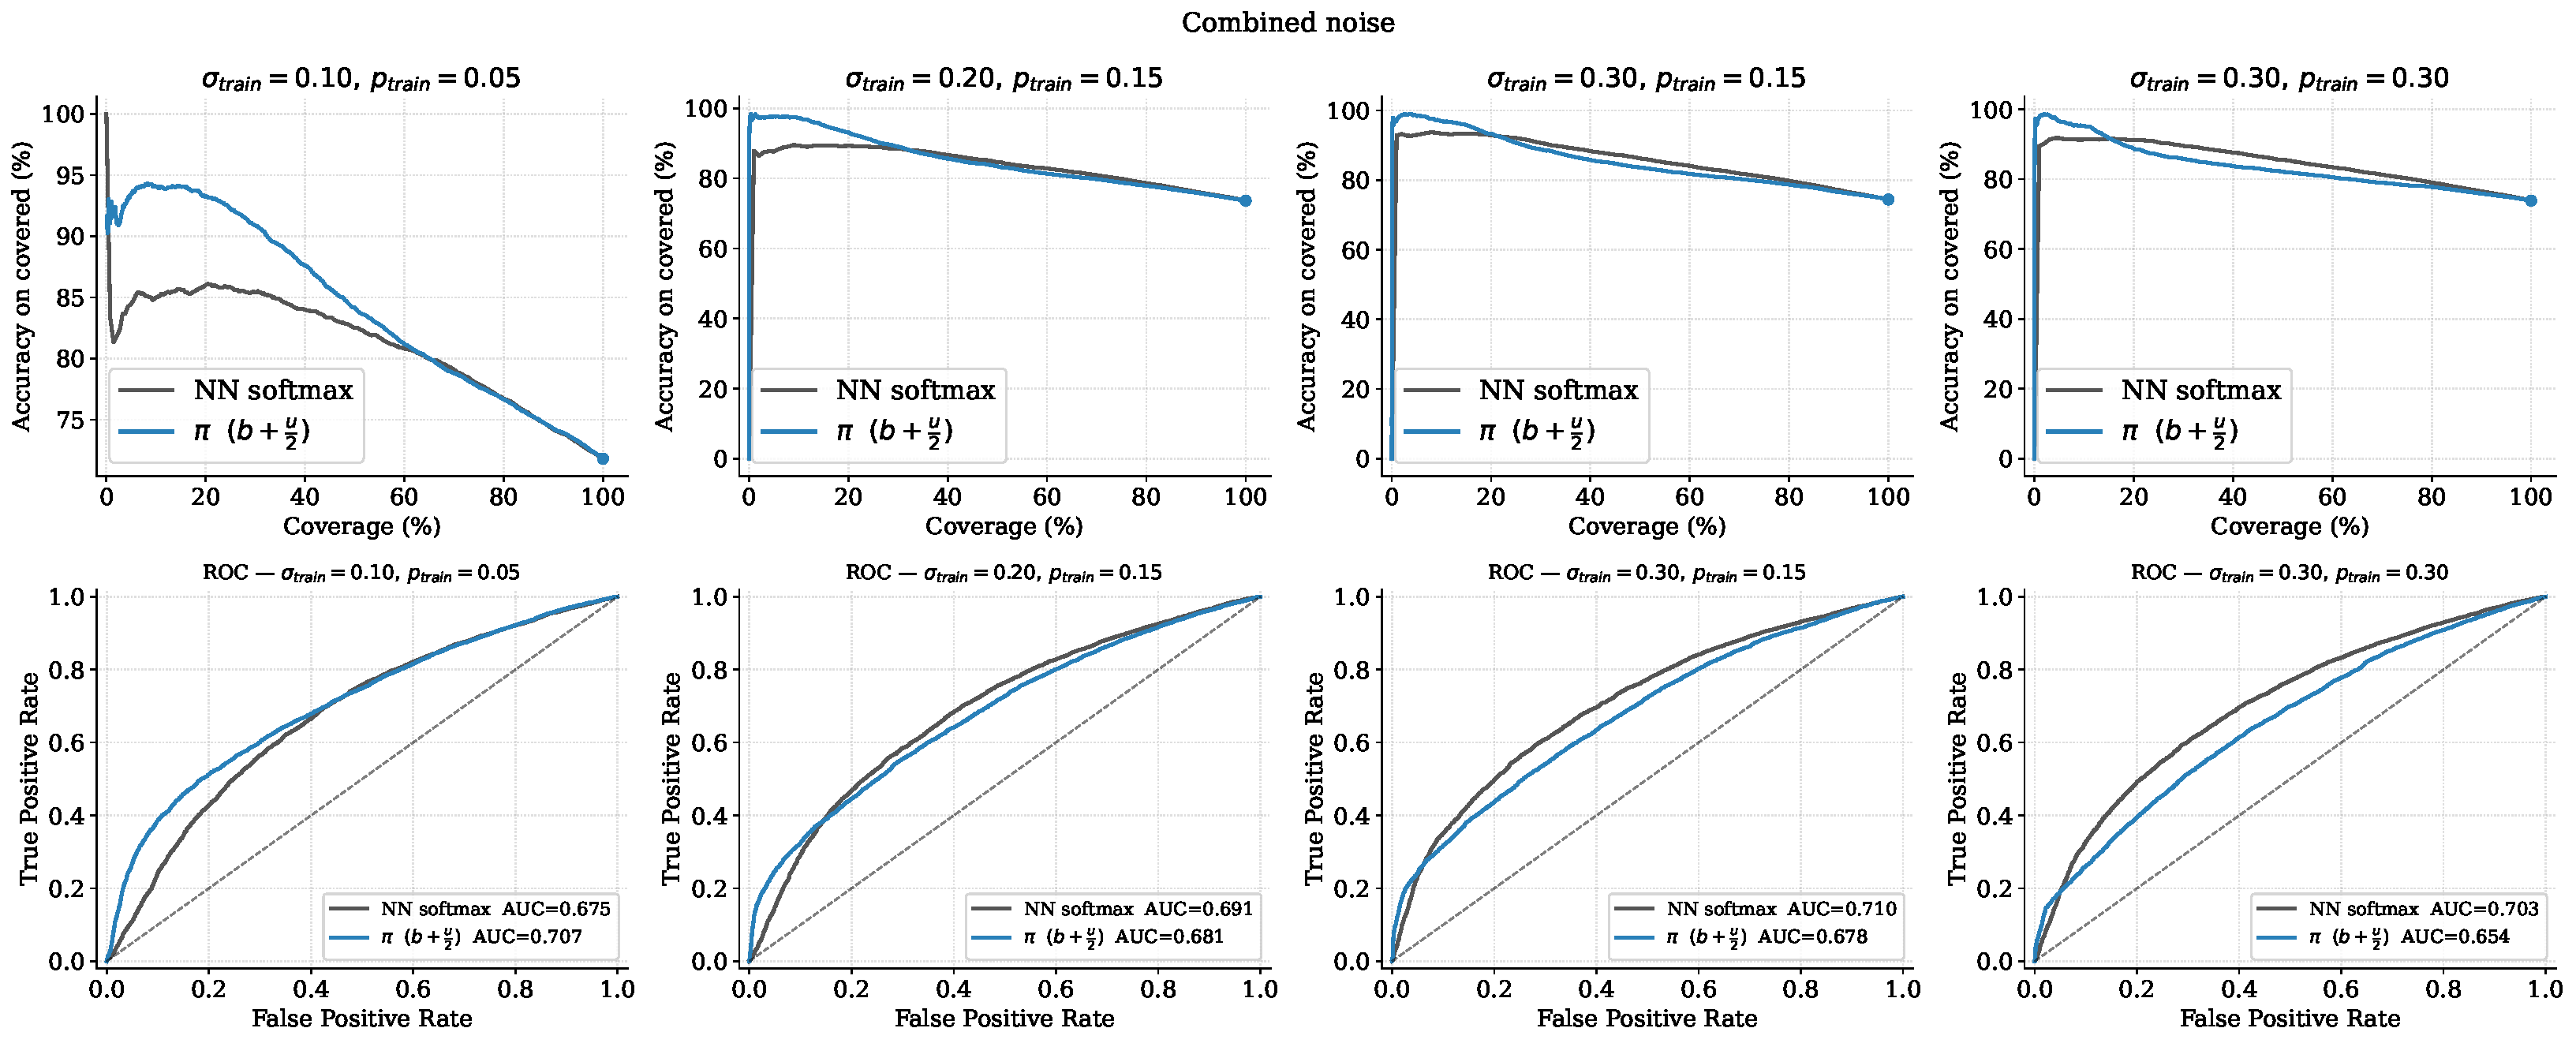
\includegraphics[width=\linewidth]{img/usecase/app/coverage_accuracy_combined.pdf}
\caption{Top: coverage--accuracy curves under combined feature and label
noise, extending \Cref{fig:coverage_accuracy_combined}, for
$(\sigma_{\text{train}}, p_{\text{train}}) \in \{(0.10, 0.05), (0.20,
0.15), (0.30, 0.15), (0.30, 0.30)\}$. Bottom: corresponding ROC curves
and AUC.}
\label{fig:app_coverage_roc_combined}
\end{figure}
 
The combined-noise condition is the one case where the ROC/AUC view
diverges from the coverage--accuracy view. At the mildest condition,
$(\sigma_{\text{train}}, p_{\text{train}}) = (0.10, 0.05)$, \ac{PaTAS}
still leads with $\text{AUC} = 0.707$ against $0.675$ for softmax,
consistent with \Cref{sec:selective_prediction}. At the three more
severe conditions, however, softmax attains a \emph{higher} AUC than
\ac{PaTAS}: $0.691$ versus $0.681$ at $(0.20, 0.15)$, $0.710$ versus
$0.678$ at $(0.30, 0.15)$, and $0.703$ versus $0.654$ at $(0.30,
0.30)$, with the gap widening as combined noise intensifies. This
indicates that, while \Cref{sec:selective_prediction} describes the two
curves as "closely overlapping" or "nearly indistinguishable" in the
low-coverage operating region typically used for selective prediction,
softmax is in fact the better \emph{global} ranking signal across the
full coverage range once both feature and label noise are
simultaneously elevated. The two views are not necessarily in tension:
AUC aggregates performance over the entire coverage range, including
high-coverage operating points of limited practical interest for
selective prediction, whereas the coverage--accuracy curves emphasize
the low-coverage regime where a practitioner would actually set the
filtering threshold. This reversal is nonetheless worth flagging
explicitly as a boundary condition on the claim that \ac{PaTAS}
provides a consistent advantage over softmax: under simultaneously
high feature and label noise, that advantage is confined to the
low-coverage region and does not extend to global ranking quality.

 


%----------------------------------------------------------------------------------------
%	BIBLIOGRAPHY
%----------------------------------------------------------------------------------------


%----------------------------------------------------------------------------------------

\end{document}  
